\documentclass[12pt]{exam}

\newcommand{\Version}{1} 
\newcommand{\Solutions}{1} 
\newcommand{\TestName}{} 

% LOAD PACKAGES
\usepackage{amsmath} % allows for align env and other things
\usepackage{amssymb} % 
\usepackage{mathtools} % allows for single apostrophe
\usepackage{enumitem} % allows for alpha lettering in enumerated lists
\usepackage{lastpage}
\usepackage{array} % for table alignments

\usepackage[T1]{fontenc}
\usepackage{tgbonum}

% TIKZ DIAGRAMS (IF NEEDED)
\usepackage{color}
\usepackage{tikz}  
\usetikzlibrary{arrows, automata} 
\usetikzlibrary{calc} 
\usepackage{pgfplots}
\pgfplotsset{compat=newest}
\usepgfplotslibrary{fillbetween}

% ADJUST MARGINS 
\usepackage[tmargin=2.0in,bmargin=1.5in]{geometry}
\geometry{margin=0.76in}

% COLORS FOR DIAGRAMS IN SOLUTIONS
\definecolor{DarkBlue}{rgb}{0.0,0.2,0.25} % 
\definecolor{DarkRed}{rgb}{0.4,0.0,0.0} % 

% HEADERS AND FOOTERS
\pagestyle{headandfoot}
\runningfooter{}{}{}
\runningheader{\textit{\TestName}}{}{\textit{Page \thepage \ of \pageref{LastPage}} }
\headheight 42pt % distance from top of page to top of header
\headsep 12pt % space between header and top of body

\newcommand{\ID}{Fill in the blanks with a dark pen or pencil. 
Using only capital letters print your \\ first name: \framebox{\strut\hspace{4.2cm}}, last name: \framebox{\strut\hspace{4.2cm}}, the remaining digits \\[2pt] of your GTID:  \framebox{\strut $9$}\framebox{\strut $0$}\framebox{\strut\hspace{0.19cm}}\framebox{\strut\hspace{0.19cm}}\framebox{\strut\hspace{0.19cm}}\framebox{\strut\hspace{0.19cm}}\framebox{\strut\hspace{0.19cm}}\framebox{\strut\hspace{0.19cm}}\framebox{\strut\hspace{0.19cm}}, the High School you attend: \framebox{\strut\hspace{5.2cm}}.}

% ADJUST FIRST LINE IN PARAGRAPH INDENTATION 
\setlength\parindent{0pt}

% FONT FORMAT
\renewcommand*\rmdefault{lmss} % change font to lat mod ss

% AUGMENTED MATRIX
\newenvironment{amatrix}[1]{%
  \left(\begin{array}{@{}*{#1}{c}|c@{}}
}{%
  \end{array}\right)
}

% SHORCUTS FOR DERIVATIVES
\newcommand{\ddt}{\frac{d}{dt}}
\newcommand{\dfdx}{\frac{df}{dx}}
\newcommand{\dfdt}{\frac{df}{dt}}
\newcommand{\dgdt}{\frac{dg}{dt}}
\newcommand{\dhdt}{\frac{dh}{dt}}
\newcommand{\dxdt}{\frac{dx}{dt}}
\newcommand{\dydt}{\frac{dy}{dt}}
\newcommand{\dzdt}{\frac{dz}{dt}}
\newcommand{\DDX}{\frac{\partial}{\partial x}}
\newcommand{\DDY}{\frac{\partial}{\partial y}}
\newcommand{\DDZ}{\frac{\partial}{\partial z}}
\newcommand{\DFDX}{\frac{\partial f}{\partial x}}
\newcommand{\DFDY}{\frac{\partial f}{\partial y}}
\newcommand{\DFDZ}{\frac{\partial f}{\partial z}}

\newcommand{\DFFDX}{\frac{\partial F}{\partial x}}
\newcommand{\DFFDY}{\frac{\partial F}{\partial y}}
\newcommand{\DFFDZ}{\frac{\partial F}{\partial z}}

\newcommand{\DZDX}{\frac{\partial z}{\partial x}}
\newcommand{\DZDY}{\frac{\partial z}{\partial y}}
\newcommand{\DFDXX}{\frac{\partial^2 f}{\partial x^2}}
\newcommand{\DFDYY}{\frac{\partial^2 f}{\partial y^2}}
\newcommand{\DFDXY}{\frac{\partial^2 f}{\partial x\partial y}}
\newcommand{\DFDYX}{\frac{\partial^2 f}{\partial y\partial x}}

\newcommand{\DXDU}{\frac{\partial x}{\partial u}}
\newcommand{\DXDV}{\frac{\partial x}{\partial v}}
\newcommand{\DYDU}{\frac{\partial y}{\partial u}}
\newcommand{\DYDV}{\frac{\partial y}{\partial v}}

\usepackage{hyperref}
\hypersetup{
    colorlinks=true,
    linkcolor=DarkBlue,
    filecolor=DarkBlue,      
    urlcolor=DarkBlue,
    pdfpagemode=FullScreen,
}

    
% --------------------------------------------------------------------
\begin{document}

% \thispagestyle{empty} % supress headers and footers for this page only
\begin{tikzpicture}[remember picture,overlay]

    % \node[opacity=1,inner sep=0pt] at (8.5,-11){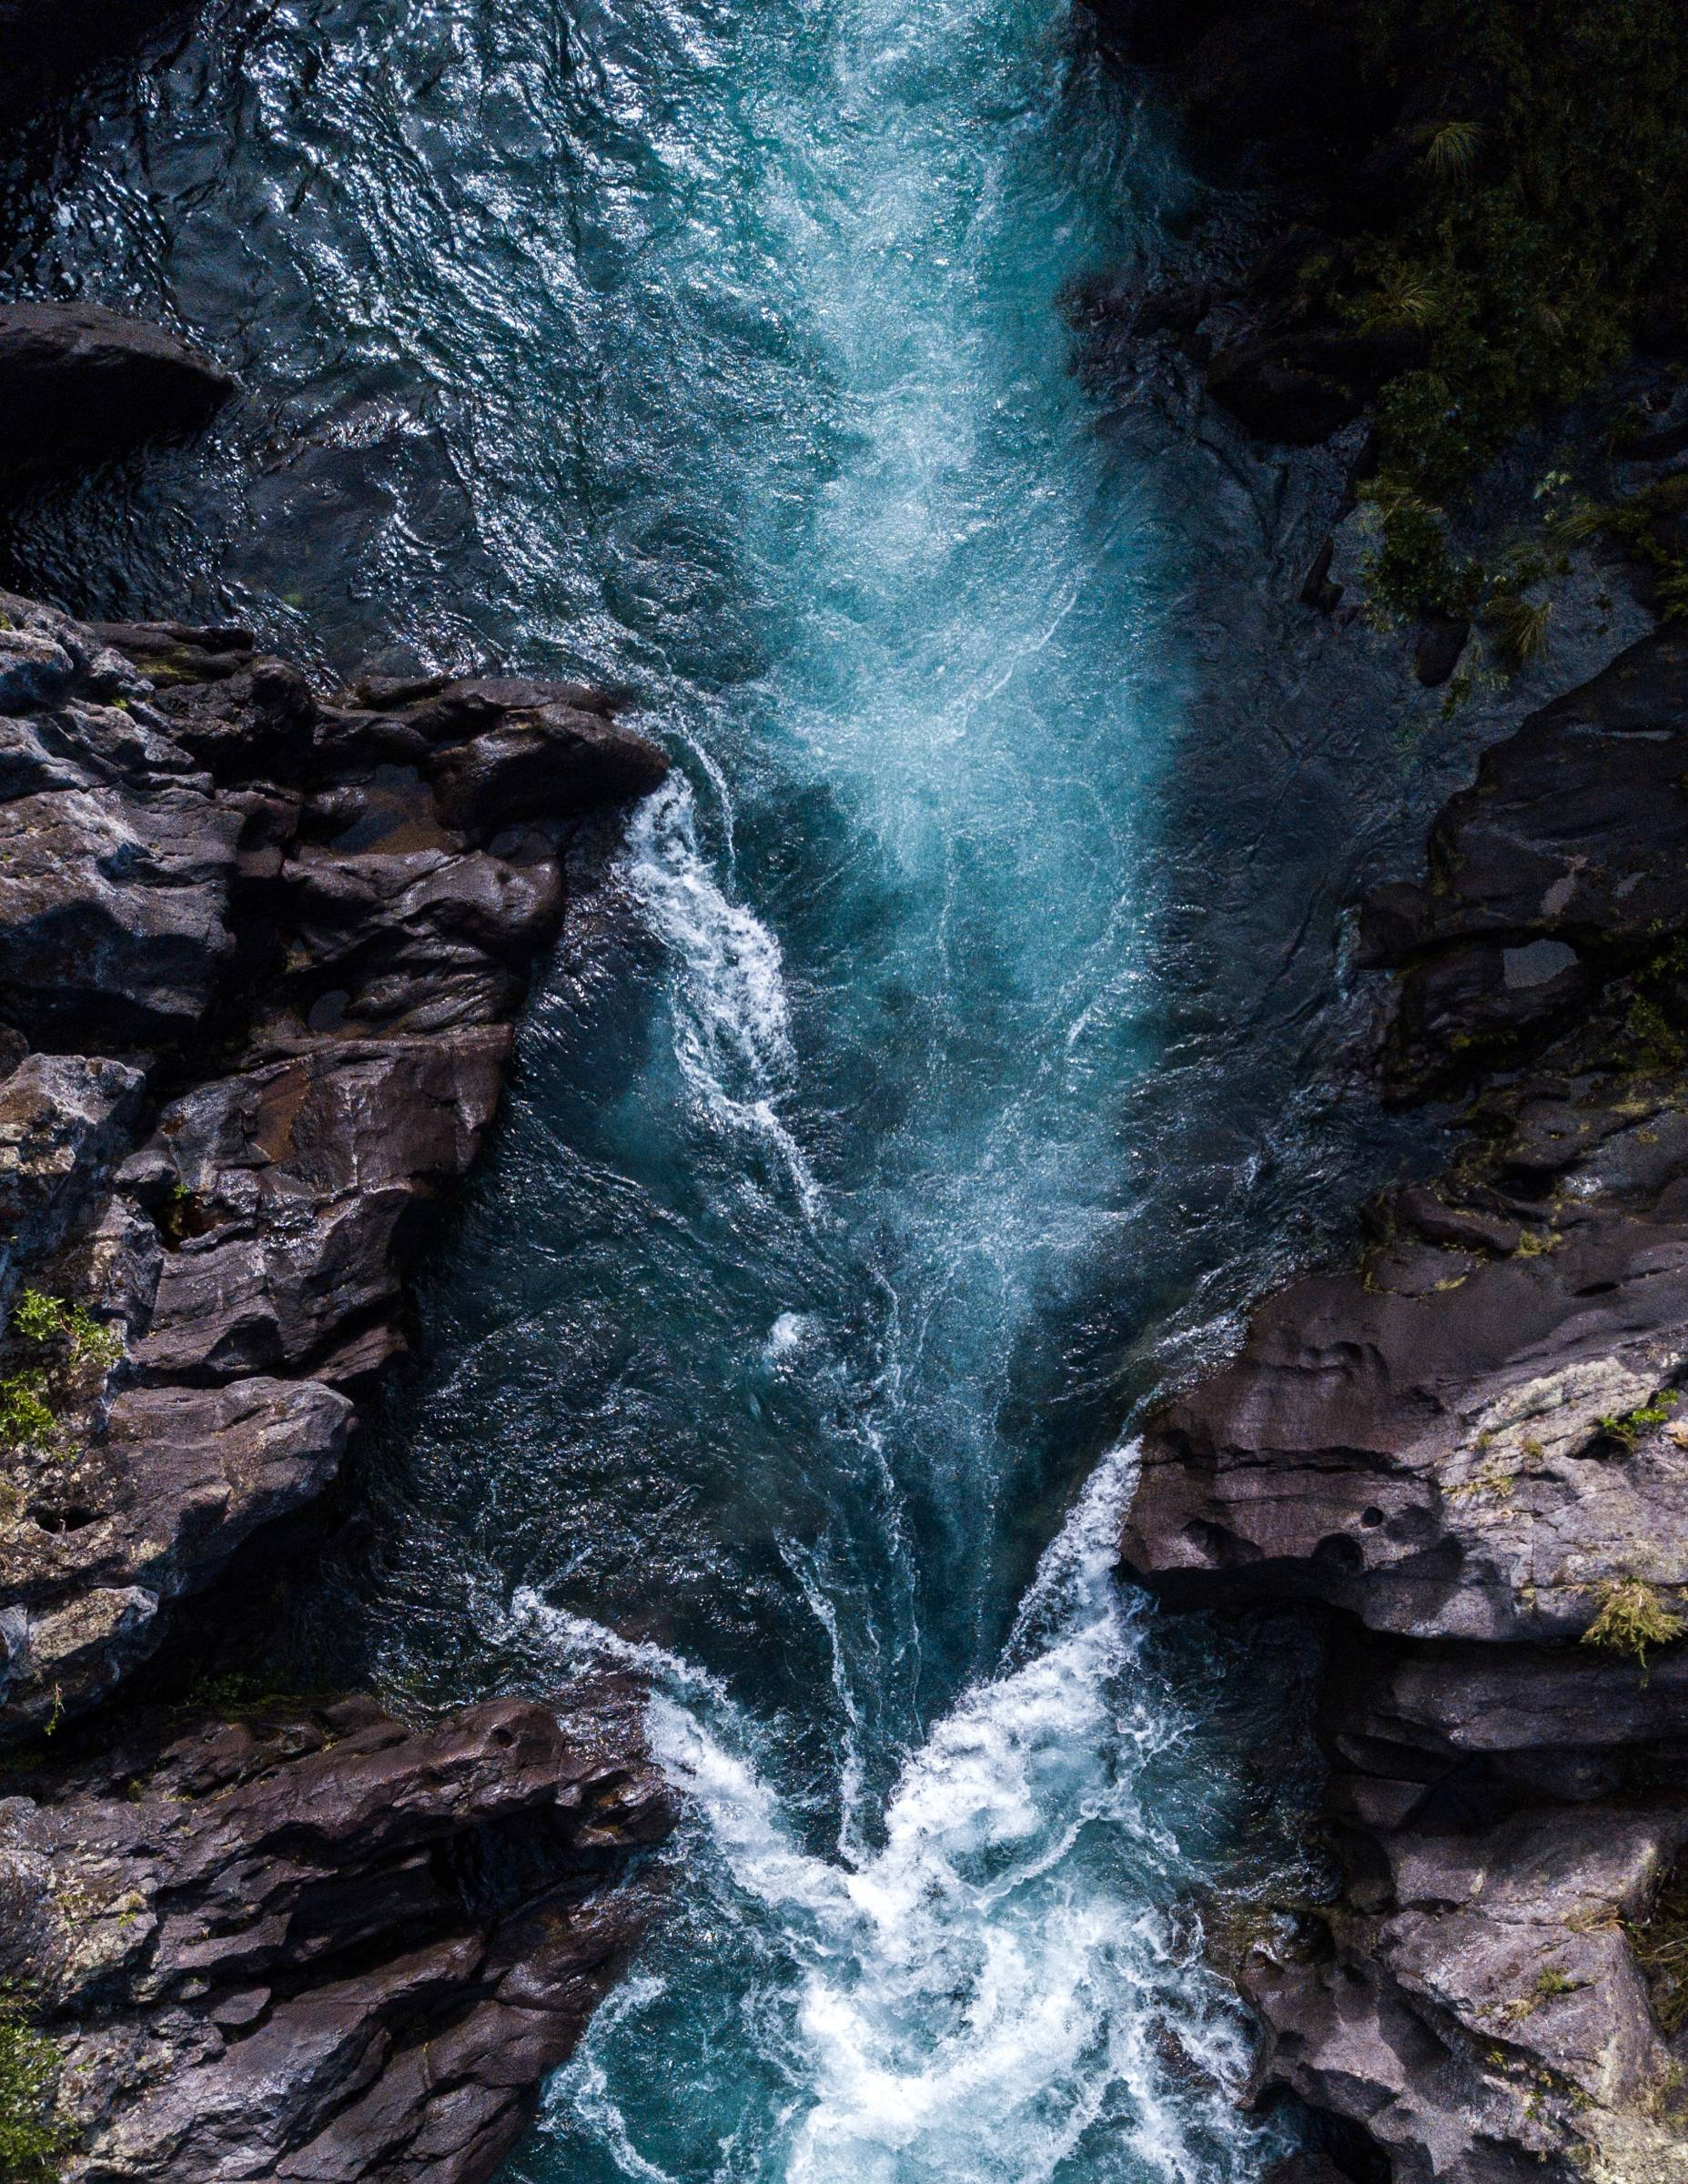
\includegraphics[width=1.08\paperwidth,height=1.05\paperheight]{202402/Exam1/JV_unsplash.jpg}};
    \node[opacity=1,inner sep=0pt] at (8.5,-11){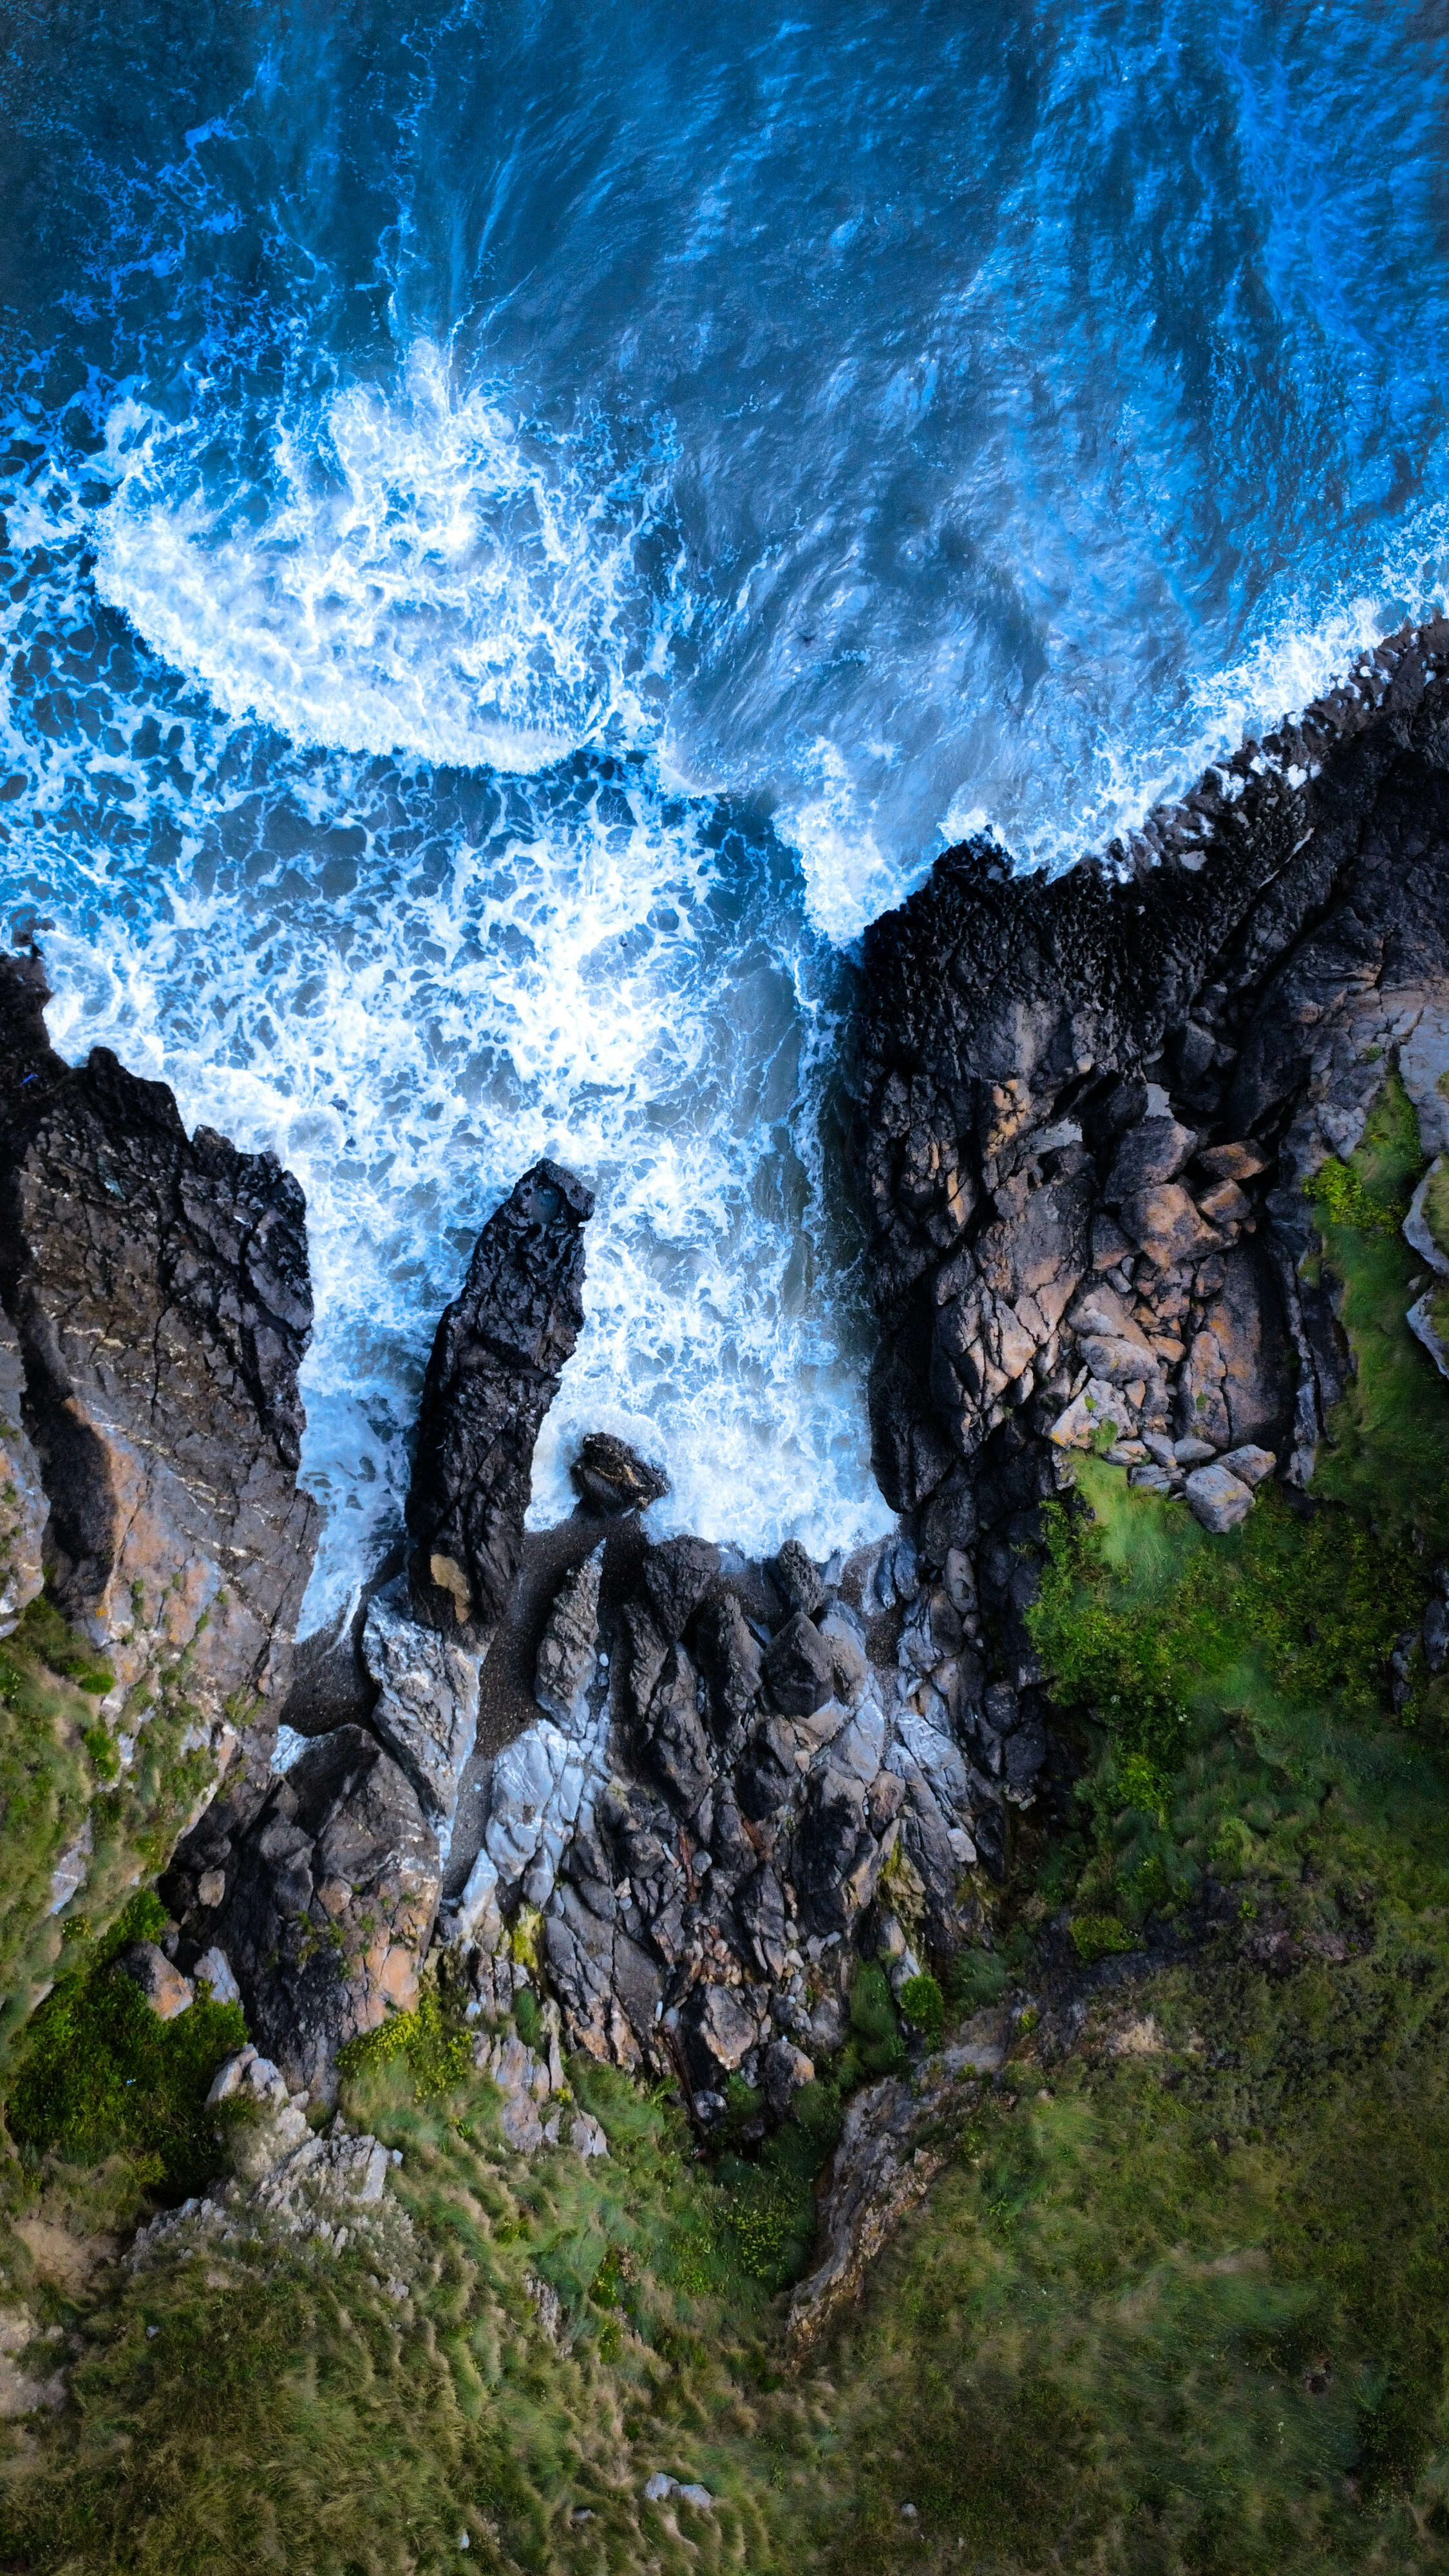
\includegraphics[width=1.08\paperwidth,height=1.05\paperheight]{202402/CoverImages/rinalds-vanags-x7-VxPpbsmM-unsplash.jpg}};
    
    \filldraw[black, opacity = 0.65] (-3, -7.25) rectangle (\paperwidth, 1.15);
    \filldraw[black, opacity = 0.65] (-3, 1.25) rectangle (\paperwidth, 1.15);
    % \filldraw[black, opacity = 0.65] (-3, -7.25) rectangle (\paperwidth, 0.15);
    \draw[] (.1,-0.3) node[right]{\begingroup{\fontfamily{qhv} 
    \fontsize{28pt}{12pt}\selectfont{\color{white} Sample Exams for the Final Exam}}\endgroup};
    \draw[] (.2,-1.6) node[right]{{\fontfamily{qhv}\selectfont {\Large \color{white} Multivariable Calculus }}};
    \draw[] (.2,-2.4) node[right]{{\fontfamily{qhv}\selectfont {\Large \color{white} MATH 2551 QH }}};        
    \draw[] (.2,-3.2) node[right]{{\fontfamily{qhv}\selectfont {\Large \color{white} Distance Math Program}}};        
    \draw[] (.2,-4.0) node[right]{{\fontfamily{qhv}\selectfont {\Large \color{white} Spring 2024 }}};        
\ifnum \Solutions=1
    \draw[] (.2,-4.8) node[right]{{\fontfamily{qhv}\selectfont {\Large \color{white} Exams with Solutions }}};        
\fi
    \draw[] (.2,-5.8) node[right]{{\fontfamily{qhv}\selectfont {\Large \color{white} Last Compiled on \today. }}};        
    
\end{tikzpicture}

\newpage

\thispagestyle{empty} % supress headers and footers for this page only

\begin{center}
{\huge \textbf{Preface}}

\vspace{24pt}
These exams are intended for use in the Georgia Tech Distance Math Program offer of the multivariable calculus course, MATH 2551. 

\vspace{24pt}

The document was created using LaTeX and was last compiled on \today. 

\vspace{24pt}

% The cover image photo is by \href{https://unsplash.com/@lukeelliscraven}{\underline{Luke Ellis-Craven}} and was downloaded from \href{https://unsplash.com/}{\underline{Unsplash.com}} on 2/15/2024.

  % The cover image photo is by \href{https://unsplash.com/@andrewtang}{\underline{Andrew Tang}} and was downloaded from \href{https://unsplash.com/}{\underline{Unsplash.com}} on 2/15/2024.


  The cover image photo is by \href{https://unsplash.com/@vanagsphotography}{\underline{Rinalds Vanags}} and was downloaded from \href{https://unsplash.com/}{\underline{Unsplash.com}} on 4/7/2024.


\end{center}

% \newpage 



% % SAMPLE A 
% \renewcommand{\Version}{1} 
% % TEST SPECIFIC INFORMATION
\ifnum \Version=1 \renewcommand{\TestName}{Year 1 MATH 2551 Exam 3 Sample A} \fi
\ifnum \Version=2 \renewcommand{\TestName}{Year 1 MATH 2551 Exam 3 Sample B} \fi
\ifnum \Version=3 \renewcommand{\TestName}{Year 1 MATH 2551 Exam 3 Sample C} \fi
\ifnum \Version=4 \renewcommand{\TestName}{Year 1 MATH 2551 Exam 3 Sample D} \fi
\ifnum \Version=5 \renewcommand{\TestName}{Year 1 MATH 2551 Exam 3 Sample E} \fi
\ifnum \Version=6 \renewcommand{\TestName}{Year 1 MATH 2551 Exam 3 Version A} \fi
\ifnum \Version=7 \renewcommand{\TestName}{Year 1 MATH 2551 Exam 3 Version B} \fi
\ifnum \Version=8 \renewcommand{\TestName}{Year 1 MATH 2551 Exam 3 Version C} \fi
\ifnum \Version=9 \renewcommand{\TestName}{Year 1 MATH 2551 Exam 3 Version D} \fi



% TITLE
\begin{center}
\ifnum \Solutions=1 {\Large {\color{DarkBlue}\textit{Solutions}}\\[6pt]}\fi
{\Large \TestName}
\end{center}

\vspace{-16pt}

\begin{center}
\textit{Work done on scratch paper will not be graded.}

\vspace{8pt}
\textbf{A Few Helpful Formulas}
\vspace{8pt}

$
\begin{array}{llllll}
    & \displaystyle x = \rho \sin\phi \cos\theta,
    & \displaystyle y = \rho \sin\phi \sin\theta,
    & \displaystyle z = \rho \cos\phi,
    & \displaystyle dV = \rho^2 \sin \phi \, d\rho \, d\phi \, d\theta,
    & \displaystyle J(u,v) = x_uy_v - y_ux_v
\end{array} 
$
\end{center}
\begin{questions}
\question[0.5] \ID

\question[7] Fill in the blanks. You do not need to show your work. 
    
\begin{parts}
    %SECTIONS 12.1 TO 12.2 (3D, vectors)



\ifnum \Version=1
\part If $P$ is the point $(2, 8, 4)$, then the distance between $P$ and the $xy$-plane is $\framebox{\strut\hspace{1cm}}$ and the distance between $P$ and the $y$-axis is $\framebox{\strut\hspace{1cm}}$. 

\ifnum \Solutions=1 {\color{DarkBlue} \textit{Answer:} the point is 4 units above the $xy$-plane, so the first distance is 4. Looking down the $y$-axis, the point is 2 units to the left of the $y$-axis and 8 units above it, so using a right-angle triangle and the Pythgorean theorem the point is $\sqrt{2^2 + 4^2} = \sqrt{20}$ units away for the $y$-axis. 
} 
\else
  
\fi
\fi


\ifnum \Version=2
\part The point on the sphere $(x-2)^2+(y-4)^2+(z-7)^2=4$ nearest to the $xy-$plane is $P=(a,b,c)$, where $a=\framebox{\strut\hspace{.8cm}}, b=\framebox{\strut\hspace{.8cm}}, c=\framebox{\strut\hspace{.8cm}}$. The radius of the sphere is $r = \framebox{\strut\hspace{.8cm}}$. 

\ifnum \Solutions=1 {\color{DarkBlue} \textit{Answer:} $a=2$, $b=4$, $c=5$, $r = 2$. \\[12pt] \textit{Solutions:} The sphere has center $(2,4,7)$ and radius $r = 2$. Because the radius is 2 and the center has $z$--coordinate $z=7$, the sphere lies above the $xy$-plane. The point on the bottom of the sphere closest to the $xy$-plane will be 2 units directly below the center. The coordinate is $(2,4,5)$, so $a=2$, $b=4$, $c=5$. 

} 
\else
  
\fi
\fi






\ifnum \Version=3
\part An equation of the plane that is perpendicular to the $x$-axis and passes through the point $P(3,4,5)$ is $\framebox{\strut\hspace{4cm}}$. 

\ifnum \Solutions=1 {\color{DarkBlue} \textit{Answer:} The plane has equation 
\begin{align}
    \vec n \cdot (\vec x - \vec x_0) & = 0
\end{align}
Where $\vec n$ is a vector normal to the plane, $\vec x_0$ is any point in the plane, and $\vec x $ is the variable vector. We can use: 
\begin{align}
    \begin{pmatrix} 1\\0 \\0 \end{pmatrix} \cdot \left( \begin{pmatrix} x\\y\\z\end{pmatrix}  - \begin{pmatrix}3\\4\\5 \end{pmatrix} \right) & = 0 \\
    x-3 &=0 \\
    x&=3
\end{align}
} 
\else
  
\fi
\fi









\ifnum \Version=4
\part The distance between the plane $x+2y+2z=2$ and the point $S(8,2,1)$ is \framebox{\strut\hspace{1cm}}. The distance between $S$ and the $yz$-plane is $\framebox{\strut\hspace{1cm}}$. 

\ifnum \Solutions=1 {\color{DarkBlue} \textit{Solutions:} A normal to the plane is $\mathbf n = \langle 1,2,2\rangle$, and $|\mathbf{n}| = \sqrt{1^2+2^2+2^2} = \sqrt{9}=3$. A point on the plane can be found by setting $y=z=0$ and solving for $x$. Doing so gives us the point $P(2,0,0)$. Then $\mathbf{PS} = \langle6,2,1\rangle$. 
\begin{align}
    d 
    = \left| \mathbf{PS} \cdot \frac{\mathbf n}{|\mathbf{n}|} \right| 
    = \frac{1}{3}\langle6,2,1\rangle \cdot \langle 1,2,2\rangle = \frac{12}{3} = 4
\end{align}
The point $S$ is 8 units away from the $yz$-plane because the point has coordinates $(8,2,1)$. So the distance between $S$ and the $yz$-plane is 8. 
}

\else

\fi
\fi

% OOOPS!! SHOULDN'T BE HERE
\ifnum \Version=5

\part The cosine of the angle between the vectors $\langle 4,0,3\rangle$  and $\langle 2,1,2\rangle$ is \framebox{\strut\hspace{1cm}}. 

\ifnum \Solutions=1 {\color{DarkBlue} \textit{Solutions:} $\displaystyle \cos\theta = \frac{\langle 4,0,3\rangle \cdot \langle 2,1,2\rangle}{\sqrt{4^2+3^2} \sqrt{2^2+2^2+1}} = \frac{8+0+6}{\sqrt{25}\cdot \sqrt9}= \frac{14}{15}$. 
}
\else
  
\fi
\fi


% OOOPS!! SHOULDN'T BE HERE
\ifnum \Version=6

\part The projection of the point $P(2,3,4)$ onto the $yz$-plane is the point $Q(c_1,c_2,c_3)$ where $c_1 = \framebox{\strut\hspace{1cm}}$, $c_2 = \framebox{\strut\hspace{1cm}}$, $c_3 = \framebox{\strut\hspace{1cm}}$.

\ifnum \Solutions=1 {\color{DarkBlue} \textit{Solutions:} the closest point on the $yz$-plane to the point $P$ will have the same $y$ and $z$ coordinates as $P$, and will have $x$-coordinate of zero. The point is $Q(0,3,4)$, so $c_1 = 0$, $c_2=3$, $c_3=4$. No need for projection formulas. 

}
\else
  
\fi
\fi







\ifnum \Version=7
\part The point on the sphere $(x-2)^2+(y-4)^2+(z-6)^2=4$ nearest to the $yz-$plane is $P=(a,b,c)$, where $a=\framebox{\strut\hspace{1cm}}, b=\framebox{\strut\hspace{1cm}}, c=\framebox{\strut\hspace{1cm}}$.

\ifnum \Solutions=1 {\color{DarkBlue} \textit{Answer:} $a=0$, $b=4$, $c=6$. \\[12pt] \textit{Solutions:} The sphere has center $(2,4,6)$ and radius $2$. Because the radius is 2 and the center has $x$--coordinate $x=2$, the sphere lies to the right of the $yz$-plane. The point on the the sphere closest to the $xy$-plane will be 2 units directly from the center. The coordinate is $(0,4,5)$, so $a=0$, $b=4$, $c=6$. 



} 
\else
  
\fi
\fi


\ifnum \Version=8 %
\part The cosine of the angle between the vectors $\langle 2,3,-6\rangle$  and $\langle 2,2,1\rangle$ is $\cos \theta = \framebox{\strut\hspace{1cm}}$. 

\ifnum \Solutions=1 {\color{DarkBlue} \textit{Answer:} $4/21$ \\[12pt] \textit{Solutions:} $\displaystyle \cos\theta = \frac{\langle 2,3,-6\rangle \cdot \langle 2,2,1\rangle}{\sqrt{2^2+3^2+6^2} \sqrt{2^2+2^2+1}} = \frac{4}{7\cdot 3}= \frac{4}{21}$. 
}
\else
  
\fi
\fi



\ifnum \Version=9

\part The midpoint of the line segment that joins points $P(1,5,2)$ and $Q(9,3,2)$ is $S(a,b,c)$, where $a=\framebox{\strut\hspace{1cm}}$, $b=\framebox{\strut\hspace{1cm}}$, $c=\framebox{\strut\hspace{1cm}}$.

\ifnum \Solutions=1 {\color{DarkBlue} \textit{Solutions:} The midpoint is found by taking the average of the corresponding coordinates of the two points. The midpoint will be the point $(5,4,2)$. The midpoint of a line was covered in Section 12.2. 
}
\else
  
\fi
\fi 


\ifnum \Version=10
\part The equation $x^2 + y^2 - 6y + z^2 + 4z = 12$ represents a sphere whose radius is $r = \framebox{\strut\hspace{1cm}}$. The center of the sphere is at the point $P(a,b,c)$ where $a = \framebox{\strut\hspace{1cm}}$, $b = \framebox{\strut\hspace{1cm}}$, c= $\framebox{\strut\hspace{1cm}}$. 

\ifnum \Solutions=1 {\color{DarkBlue} \textit{Answer:} Completing the square and rearranging like terms: 
\begin{align}
    x^2 + y^2 - 6y + z^2 + 4z &= 12 \\
    x^2 + (y^2 - 6y +9 - 9) + (z^2 + 4z + 4 - 4 )&= 12 \\
    x^2 + (y -3)^2 + (z + 2)^2 - 9 - 4 &= 12 \\
    x^2 + (y -3)^2 + (z + 2)^2 &= 25 
\end{align}
The sphere has radius 5 and is centered at the point $(0,3,-2)$. 

} 
\else
  
\fi
\fi
    % SECTION 14.2

\ifnum \Version=1
    % THOMAS 14.1
    
    \part Consider the function $\displaystyle f(x,y) =  \frac{4x}{x^2+2x+y^2}$.

    \begin{enumerate}
        \item[i)] The range of $f(x,y)$ is \framebox{\strut\hspace{2cm}}.
        \item[ii)] Evaluate the following limit, if possible. If the limit does not exist, write DNE. $$\lim_{(x,y) \to (0,0)} f(x,y) = \framebox{\strut\hspace{1cm}}$$
        \item[iii)] An example of a point where the function $f(x,y)$ is not continuous is the point $P(a,b)$ where $a = \framebox{\strut\hspace{1cm}}$, $b = \framebox{\strut\hspace{1cm}}$.         
    \end{enumerate}
    \ifnum \Solutions=1 
    
    {\color{DarkBlue} 
    Solutions for each part are as follows. 
    \begin{itemize}
        \item[\textbf{i)}:] Note that on the $x$-axis, $y=0$ and the function is
        $$f(x,0) = \frac{4x}{x^2+2x+0} = \frac{4}{x+2}$$
        So $f$ can take on any real value except zero on the $x-$axis. Can $f$ be zero? Note also that $f(x,y)$ is equal to zero for any point $(0,y)$ and $y \ne 0$.  So the range is $\mathbb R$.

        \item[\textbf{ii)}:]  To determine the limit of the function \(f(x, y) = \frac{4x}{x^2 + 2x + y^2}\) as \(x\) and \(y\) approach zero, we can consider the limit along different paths. Let's examine the limit along the \(x\)-axis (\(y = 0\)) and the \(y\)-axis (\(x = 0\)) separately.
        Along the \(x\)-axis (\(y = 0\)):
           \[ \lim_{(x,0)\to(0,0)} \frac{4x}{x^2 + 2x + 0^2} = \lim_{x\to0} \frac{4x}{x^2 + 2x} = \lim_{x\to0} \frac{4x}{x(x + 2)} = \lim_{x\to0} \frac{4}{x + 2} = \lim_{x\to0} \frac{4}{x + 2} = 2 \]
        
            Along the \(y\)-axis (\(x = 0\)):
           \[ \lim_{(0,y)\to(0,0)} \frac{4 \cdot 0}{0^2 + 2 \cdot 0 + y^2} = 0 \]
        
        Now, since the limit along the \(x\)-axis is different from the limit along the \(y\)-axis, the overall limit as \((x, y)\) approaches \((0, 0)\) does not exist. The limit depends on the direction of approach and gives different results along different paths. The answer is DNE. 

        \item[\textbf{iii)}:] Recall that a function $f(x, y)$ is continuous at the point $P(x_0 , y_0 )$ if all three of the following conditions are met. 
        \begin{enumerate}
            \item $f$ is defined at $P$. 
            \item The limit $\displaystyle \lim_{(x,y) \to (x_0,y_0)}f(x,y)$ exists. 
            \item $\displaystyle \lim_{(x,y) \to (x_0,y_0)}f(x,y) = f(x_0,y_0)$.  
        \end{enumerate}
    
        Applying this definition, we can identify a point where the function is not continuous in a few different ways. 
        \begin{itemize}
            \item We found in the previous part that the limit at the origin does not exist, so we could use $a = b = 0$. 
            \item We can also identify a point where the function is not continuous by selecting any point where the function is not defined. Our function is not defined when the denominator is zero and the numerator is non-zero. This corresponds to the set of points where     
        $$x^2+2x+y^2 = 0$$
        Any point that satisfies this relationship is sufficient. One such point is the origin, $(0,0)$. So we can use $a = b = 0$. But there are many other points we can use. 
        \end{itemize}
        
    \end{itemize}

    

    }
    \else
    
    \fi
\fi




\ifnum \Version=2
    % THOMAS 14.1
    
    \part Consider the function $f(x,y) = \sqrt{x^2+y^2 - 1}$.
    \begin{enumerate}
        \item[i)] Where is $f(x,y)$ continuous? $ \framebox{\strut\hspace{3cm}}$. 
        \item[ii)] As $(x,y) \to (1,0)$, $f(x,y) \to \framebox{\strut\hspace{1cm}}$. If the limit does not exist write DNE. 
    \end{enumerate}
    \ifnum \Solutions=1 
    
    {\color{DarkBlue} 
        
    \textbf{i)}: Recall that a function $f(x, y)$ is continuous at the point $P(x_0 , y_0 )$ if

    \begin{enumerate}
        \item $f$ is defined at $P$. 
        \item The limit $\displaystyle \lim_{(x,y) \to (x_0,y_0)}f(x,y)$ exists. 
        \item $\displaystyle \lim_{(x,y) \to (x_0,y_0)}f(x,y) = f(x_0,y_0)$.  
    \end{enumerate}

    Also, we say that function is \textbf{continuous} if it is continuous at every point of its domain. \\[6pt] 

    This particular function is continuous everywhere on its domain. Its domain is the set $x^2+y^2 \ge 1$. So we can write the answer as $$x^2+y^2 \ge 1$$
    
    \textbf{ii)}: Substituting the limit point into $f(x,y)$ gives 
    $$\sqrt{1^2+ 0^2 - 1} = 0$$
    The answer is $0$. \\[6pt]   
    \textbf{Additional Solution Note:} You might be wondering: the limit point is at the boundary of the domain, so how might that affect the limit? Because of the way a limit is defined, for the limit to exist we only need to obtain the same value along any path \textbf{in the domain }that leads to the limit point. Which it does, because $f$ is continuous. So the limit exists and is zero. 
    }
    \else
    
    \fi
\fi








\ifnum \Version=3
    % THOMAS 14.1
    
    \part Evaluate the following limits, if possible. If the limit does not exist, write DNE. 
    \begin{enumerate}
        \item[i)] Let $\displaystyle f(x,y) = \frac{x^2-2xy + y^2}{x-y}$, with $x\ne y$. As $(x,y) \to (1,1)$, $f(x,y) \to \framebox{\strut\hspace{1cm}}$. 
        \item[ii)] Let $\displaystyle g(x,y) = \cos\left(\frac{x^2+y^2}{x+y+1}\right)$. As $(x,y) \to (0,0)$, $g(x,y) \to \framebox{\strut\hspace{1cm}}$. 
    \end{enumerate}
    \ifnum \Solutions=1 
    
    {\color{DarkBlue} 
        
    \textbf{i)}: substituting the limit point into $f(x,y)$ gives an indeterminant form $0/0$. But we can factor the numerator to express in another form. 
    $$f(x,y) = \frac{x^2-2xy + y^2}{x-y} = \frac{(x-y)^2}{x-y} = \frac{x-y}{1}= x-y$$
    Substituting the limit point now gives us that $f \to 0$. 
    
    \textbf{ii)}: substituting the limit point into $g(x,y)$ gives 
    $$g(0,0) = \cos\left(\frac{0}{0+1}\right) = \cos\left(0\right) = 1$$
    }
    \else
    
    \fi
\fi


\ifnum \Version=4
    % THOMAS 14.1
    
    \part Evaluate the following limits, if possible. If the limit does not exist, write DNE. 
    \begin{enumerate}
        \item[i)] Let $\displaystyle f(x,y) = \frac{x^2-y^2}{x-y}$, with $x\ne y$. As $(x,y) \to (1,1)$, $f(x,y) \to \framebox{\strut\hspace{1cm}}$. 
        \item[ii)] Let $\displaystyle g(x,y) = \frac{x^2+xy}{xy}$. As $(x,y) \to (0,0)$, $g(x,y) \to \framebox{\strut\hspace{1cm}}$. 
    \end{enumerate}
    \ifnum \Solutions=1 
    
    {\color{DarkBlue} 
        
    \textbf{i)}: Substituting the limit point into $f(x,y)$ gives an indeterminant form $0/0$. But we can factor the numerator to express in another form. 
    $$f(x,y) = \frac{x^2-y^2}{x-y} = \frac{(x+y)(x-y)}{x-y} = \frac{x+y}{1}= x+y$$
    Substituting the limit point now gives us that $f \to 2$. 
    
    \textbf{ii)}: Substituting the limit point into $g(x,y)$ gives an indeterminant form $0/0$. But we can consider linear paths that pass through the limit point, $y=kx$, with $k\in \mathbb R$. Our limit becomes
    $$g(x,y=kx) = \frac{x^2+x(kx)}{x(kx)} = \frac{x^2(1+k)}{kx^2} = \frac{1+k}{k} = \frac1k + 1$$
    The value of the limit depends on $k$, so the limit does not exist. The answer is DNE. 
    }
    \else
    
    \fi
\fi




\ifnum \Version=5
    % THOMAS 14.1
    
    \part Evaluate the following limits, if possible. If the limit does not exist, write DNE.
    \begin{enumerate} 
        \item[i)] Let $\displaystyle f(x,y) = \frac{x+y-9}{\sqrt{x+y}-3}$, with $x\ne y$. As $(x,y) \to (3,6)$, $f(x,y) \to \framebox{\strut\hspace{1cm}}$. 
        \item[ii)] Let $\displaystyle g(x,y) = \frac{x^4}{x^4+y^2}$. As $(x,y) \to (0,0)$, $g(x,y) \to \framebox{\strut\hspace{1cm}}$. 
    \end{enumerate}
    \ifnum \Solutions=1 
    
    {\color{DarkBlue} 
        
    \textbf{i)}: Substituting the limit point into $f(x,y)$ gives an indeterminant form $0/0$. But we can rationalize the denominator to express $f$ in another form. 
    \begin{align}
        f(x,y) 
        &= \frac{x+y-9}{\sqrt{x+y}-3} \\
        &= \frac{x+y-9}{\sqrt{x+y}-3}\frac{\sqrt{x+y}+3}{\sqrt{x+y}+3}\\
        &= \frac{x+y-9}{x+y-9}\frac{\sqrt{x+y}+3}{1}\\
        &= \sqrt{x+y}+3
    \end{align}
    
    Then 
    \begin{align}
        \lim_{(x,y) \to (3,6)} f(x,y) = \lim_{(x,y) \to (3,6)} \sqrt{x+y}+3 = 6
    \end{align}
    Substituting the limit point now gives us that $f \to 6$. 
    
    \textbf{ii)}: To evaluate the limit of the function \( g(x, y) = \frac{x^4}{x^4 + y^2} \) as \((x, y)\) approaches the origin \((0, 0)\), we can consider approaching along different paths. If the limit is the same along all paths, then the limit exists; otherwise, it does not.

    Let's consider two paths: along the x-axis (\(y = 0\)) and along the y-axis (\(x = 0\)).
    
    \begin{itemize}
        \item Along the x-axis (\(y = 0\)):
       \[ \lim_{{(x, y) \to (0, 0)}} \frac{x^4}{x^4 + y^2} = \lim_{{x \to 0}} \frac{x^4}{x^4} = \lim_{{x \to 0}} 1 = 1 \]
       \item Along the y-axis (\(x = 0\)):
       \[ \lim_{{(x, y) \to (0, 0)}} \frac{x^4}{x^4 + y^2} = \lim_{{y \to 0}} \frac{0}{y^2} = 0 \]
    \end{itemize}

    Since the limits along different paths are not the same, the limit of \( g(x, y) \) as \((x, y)\) approaches the origin does not exist. The answer is DNE. 
    }
    \else
    
    \fi
\fi





\ifnum \Version=6
    % THOMAS 14.1
    
    \part Evaluate the following limits, if possible. If the limit does not exist, write DNE. 
    \begin{enumerate}
        \item[i)] Let $\displaystyle f(x,y) = \frac{x+y}{x}$. As $(x,y) \to (0,0)$, $f(x,y) \to \framebox{\strut\hspace{1cm}}$. 
        \item[ii)] Let $\displaystyle g(x,y) = \cos\left(\frac{x^2+y^2}{x+y+1}\right)$. As $(x,y) \to (0,0)$, $g(x,y) \to \framebox{\strut\hspace{1cm}}$. 
    \end{enumerate}
    \ifnum \Solutions=1 
    
    {\color{DarkBlue} 
        
    \textbf{i)}: substituting the limit point into $f(x,y)$ gives an indeterminant form $0/0$. But we can consider linear paths that pass through the limit point, $y=kx$, with $k\in \mathbb R$. Our limit becomes
    $$f(x,y=kx) = \frac{x+ (kx)}{x} = \frac{x(1+k)}{x} = 1+k$$
    The value of the limit depends on $k$, so the limit does not exist. The answer is DNE. 
    
    \textbf{ii)}: substituting the limit point into $g(x,y)$ gives 
    $$g(0,0) = \cos\left(\frac{0}{0+1}\right) = \cos\left(0\right) = 1$$
    }
    \else
    
    \fi
\fi





\ifnum \Version=7
    % THOMAS 14.1
    
    \part Evaluate the following limits, if possible. If the limit does not exist, write DNE. 
    \begin{enumerate}
        \item[i)] Let $\displaystyle f(x,y) = \frac{x^2 + 2xy + y^2}{x+y}$, with $x+y\ne 0$. As $(x,y) \to (0,0)$, $f(x,y) \to \framebox{\strut\hspace{1cm}}$. 
        \item[ii)] Let $\displaystyle g(x,y) = \frac{x^2 - 2y}{x-y}$, with $x\ne y$. As $(x,y) \to (0,0)$, $g(x,y) \to \framebox{\strut\hspace{1cm}}$.  
    \end{enumerate}
    \ifnum \Solutions=1 
    
    {\color{DarkBlue} 
        
    \textbf{i)}: substituting the limit point into $f(x,y)$ gives an indeterminant form $0/0$. But we can factor the numerator to express in another form. 
    $$f(x,y) 
    = \frac{x^2 + 2xy + y^2}{x+y} 
    = \frac{(x+y)^2}{x+y}
    = x+y
    $$
    Substituting the limit point now gives us that $f \to 0$. 
    
    \textbf{ii)}: substituting the limit point into $g(x,y)$ gives an indeterminant form. Let's consider two paths: along the $x$-axis (\(y = 0\)) and along the $y$-axis (\(x = 0\)).
    
    \begin{itemize}
        \item Along the x-axis (\(y = 0\)):
       \[ \lim_{{(x, y) \to (0, 0)}} \frac{x^2 - 2y}{x-y} = \lim_{{x \to 0}} \frac{x^2 }{x} = \lim_{{x \to 0}} x = 0 \]
       \item Along the y-axis (\(x = 0\)):
       \[ \lim_{{(x, y) \to (0, 0)}} \frac{x^2 - 2y}{x-y} = \lim_{{y \to 0}} \frac{- 2y}{-y} = 2 \]
    \end{itemize}

    Since the limits along different paths are not the same, the limit of \( g(x, y) \) as \((x, y)\) approaches the origin does not exist. The answer is DNE. 
    }
    \else
    
    \fi
\fi


\ifnum \Version=8
    % THOMAS 14.1
    
    \part Evaluate the following limits, if possible. If the limit does not exist, write DNE. 
    \begin{enumerate}
        \item[i)] Let $\displaystyle f(x,y) = \frac{x^2 - y^2}{x-y}$, with $x-y\ne 0$. As $(x,y) \to (0,0)$, $f(x,y) \to \framebox{\strut\hspace{1cm}}$. 
        \item[ii)] Let $\displaystyle g(x,y) = \frac{x^2 - 4y}{x^2-y}$, with $x\ne y$. As $(x,y) \to (0,0)$, $g(x,y) \to \framebox{\strut\hspace{1cm}}$.  
    \end{enumerate}
    \ifnum \Solutions=1 
    
    {\color{DarkBlue} 
        
    \textbf{i)}: substituting the limit point into $f(x,y)$ gives an indeterminant form $0/0$. But we can factor the numerator to express in another form. 
    $$f(x,y) 
    = \frac{x^2 - y^2}{x-y} 
    = \frac{(x+y)(x-y)}{x-y}
    = x+y
    $$
    Substituting the limit point now gives us that $f \to 0$. 
    
    \textbf{ii)}: substituting the limit point into $g(x,y)$ gives an indeterminant form. Let's consider two paths: along the $x$-axis (\(y = 0\)) and along the $y$-axis (\(x = 0\)).
    
    \begin{itemize}
        \item Along the x-axis (\(y = 0\)):
       \[ \lim_{{(x, y) \to (0, 0)}} \frac{x^2 - 4y}{x^2-y} = \lim_{{x \to 0}} \frac{x^2 }{x^2} = \lim_{{x \to 0}} 1 = 1 \]
       \item Along the y-axis (\(x = 0\)):
       \[ \lim_{{(x, y) \to (0, 0)}} \frac{x^2 - 4y}{x^2-y} = \lim_{{y \to 0}} \frac{- 4y}{-y} = 4 \]
    \end{itemize}

    Since the limits along different paths are not the same, the limit of \( g(x, y) \) as \((x, y)\) approaches the origin does not exist. The answer is DNE. 
    }
    \else
    
    \fi
\fi






\ifnum \Version=9
    % THOMAS 14.1
    
    \part Evaluate the following limits, if possible. If the limit does not exist, write DNE. 
    \begin{enumerate}
        \item[i)] Let $\displaystyle f(x,y) = \frac{x+y-4}{\sqrt{x+y}-2}$. As $(x,y) \to (2,2)$, $f(x,y) \to \framebox{\strut\hspace{1cm}}$. 
        \item[ii)] Let $\displaystyle g(x,y) = \frac{x^4 - y^2}{x^4+y^2}$. As $(x,y) \to (0,0)$, $g(x,y) \to \framebox{\strut\hspace{1cm}}$.  
    \end{enumerate}
    \ifnum \Solutions=1 
    
    {\color{DarkBlue} 
        
    \textbf{i)}: substituting the limit point into $f(x,y)$ gives an indeterminant form $0/0$. But we can rationalize the denominator to express in another form. 
    \begin{align}
        f(x,y) 
        &= \frac{x+y-4}{\sqrt{x+y}-2} \\
        &= \frac{x+y-4}{\sqrt{x+y}-2} \cdot \frac{\sqrt{x+y}+2}{\sqrt{x+y}+2} \\
        &= \frac{x+y-4}{x+y-4} \cdot \frac{\sqrt{x+y}+2}{1} \\
        &= \sqrt{x+y}+2
    \end{align}
    Substituting the limit point now gives us that $f \to 4$. 
    
    \textbf{ii)}: substituting the limit point into $g(x,y)$ gives an indeterminant form. Let's consider two paths: along the $x$-axis (\(y = 0\)) and along the $y$-axis (\(x = 0\)).
    
    \begin{itemize}
        \item Along the $x$-axis (\(y = 0\)):
       \[ \lim_{{(x, y) \to (0, 0)}} \frac{x^4 - y^2}{x^4+y^2} = \lim_{{x \to 0}} \frac{x^4 }{x^4} = \lim_{{x \to 0}} 1 = 1 \]
       \item Along the $y$-axis (\(x = 0\)):
       \[ \lim_{{(x, y) \to (0, 0)}} \frac{x^4 - y^2}{x^4+y^2} = \lim_{{y \to 0}} \frac{ - y^2}{+y^2} = -1 \]
    \end{itemize}

    Since the limits along different paths are not the same, the limit of \( g(x, y) \) as \((x, y)\) approaches the origin does not exist. The answer is DNE. 
    }
    \else
    
    \fi
\fi



\ifnum \Version=10
    % THOMAS 14.1
    
    \part Evaluate the following limits, if possible. If the limit does not exist, write DNE. 
    \begin{enumerate}
        \item[i)] Let $\displaystyle f(x,y) = \frac{x+y-4}{\sqrt{x+y}-2}$. As $(x,y) \to (2,2)$, $f(x,y) \to \framebox{\strut\hspace{1cm}}$. 
        \item[ii)] Let $\displaystyle g(x,y) = \frac{x^4 - y^2}{x^4+y^2}$. As $(x,y) \to (0,0)$, $g(x,y) \to \framebox{\strut\hspace{1cm}}$.  
    \end{enumerate}
    \ifnum \Solutions=1 
    
    {\color{DarkBlue} 
        
    \textbf{i)}: substituting the limit point into $f(x,y)$ gives an indeterminant form $0/0$. But we can rationalize the denominator to express in another form. 
    \begin{align}
        f(x,y) 
        &= \frac{x+y-4}{\sqrt{x+y}-2} \\
        &= \frac{x+y-4}{\sqrt{x+y}-2} \cdot \frac{\sqrt{x+y}+2}{\sqrt{x+y}+2} \\
        &= \frac{x+y-4}{x+y-4} \cdot \frac{\sqrt{x+y}+2}{1} \\
        &= \sqrt{x+y}+2
    \end{align}
    Substituting the limit point now gives us that $f \to 4$. 
    
    \textbf{ii)}: substituting the limit point into $g(x,y)$ gives an indeterminant form. Let's consider two paths: along the $x$-axis (\(y = 0\)) and along the $y$-axis (\(x = 0\)).
    
    \begin{itemize}
        \item Along the $x$-axis (\(y = 0\)):
       \[ \lim_{{(x, y) \to (0, 0)}} \frac{x^4 - y^2}{x^4+y^2} = \lim_{{x \to 0}} \frac{x^4 }{x^4} = \lim_{{x \to 0}} 1 = 1 \]
       \item Along the $y$-axis (\(x = 0\)):
       \[ \lim_{{(x, y) \to (0, 0)}} \frac{x^4 - y^2}{x^4+y^2} = \lim_{{y \to 0}} \frac{ - y^2}{+y^2} = -1 \]
    \end{itemize}

    Since the limits along different paths are not the same, the limit of \( g(x, y) \) as \((x, y)\) approaches the origin does not exist. The answer is DNE. 
    }
    \else
    
    \fi
\fi



\ifnum \Version=11
    % THOMAS 14.1
    
    \part Evaluate the following limits, if possible. If the limit does not exist, write DNE. 
    \begin{enumerate}
        \item[i)] Let $\displaystyle f(x,y) = \frac{x^2 - y^2}{x-y}$, with $x-y\ne 0$. As $(x,y) \to (0,0)$, $f(x,y) \to \framebox{\strut\hspace{1cm}}$. 
        \item[ii)] Let $\displaystyle g(x,y) = \frac{x^2 - 4y}{x^2-y}$, with $x\ne y$. As $(x,y) \to (0,0)$, $g(x,y) \to \framebox{\strut\hspace{1cm}}$.  
    \end{enumerate}
    \ifnum \Solutions=1 
    
    {\color{DarkBlue} 
        
    \textbf{i)}: substituting the limit point into $f(x,y)$ gives an indeterminant form $0/0$. But we can factor the numerator to express in another form. 
    $$f(x,y) 
    = \frac{x^2 - y^2}{x-y} 
    = \frac{(x+y)(x-y)}{x-y}
    = x+y
    $$
    Substituting the limit point now gives us that $f \to 0$. 
    
    \textbf{ii)}: substituting the limit point into $g(x,y)$ gives an indeterminant form. Let's consider two paths: along the $x$-axis (\(y = 0\)) and along the $y$-axis (\(x = 0\)).
    
    \begin{itemize}
        \item Along the x-axis (\(y = 0\)):
       \[ \lim_{{(x, y) \to (0, 0)}} \frac{x^2 - 4y}{x^2-y} = \lim_{{x \to 0}} \frac{x^2 }{x^2} = \lim_{{x \to 0}} 1 = 1 \]
       \item Along the y-axis (\(x = 0\)):
       \[ \lim_{{(x, y) \to (0, 0)}} \frac{x^2 - 4y}{x^2-y} = \lim_{{y \to 0}} \frac{- 4y}{-y} = 4 \]
    \end{itemize}

    Since the limits along different paths are not the same, the limit of \( g(x, y) \) as \((x, y)\) approaches the origin does not exist. The answer is DNE. 
    }
    \else
    
    \fi
\fi

    % SECTIONS 12.5
\ifnum \Version=1
\part The cosine of the angle between the planes $2x-2y-z=1$ and $x+2y+2z=2$ is \framebox{\strut\hspace{1cm}}.

\ifnum \Solutions=1 {\color{DarkBlue} \textit{Answer:} $-4/9$ \\[12pt] \textit{Solutions:} 

$$\cos \theta = \frac{\langle 2,-2,-1\rangle \cdot \langle 1,2,2\rangle}{\sqrt{2^2+2^2+1^2}\sqrt{1^2+2^2+2^2}}= \frac{-4}{9}$$

} 
\else
  
\fi
\fi

\ifnum \Version=2
\part The distance between the plane $x+4y+8z=1$ and the point $S(4,0,0)$ is \framebox{\strut\hspace{1cm}}.

\ifnum \Solutions=1 {\color{DarkBlue} \textit{Answer:} $1/3$ \\[12pt] \textit{Solutions:} A normal to the plane is $\mathbf n = \langle 1,4,8\rangle$, and $|\mathbf{n}| = \sqrt{1^2+4^2+8^2} = \sqrt{81}=9$. A point on the plane can be found by setting $y=z=0$ and solving for $x$. Doing so gives us the point $P(1,0,0)$. Then $\mathbf{PS} = \langle3,0,0\rangle$. The distance is 
\begin{align}
    d = \left| \mathbf{PS} \cdot \frac{\mathbf n}{|\mathbf{n}|} \right| = \frac{1}{9}\langle3,0,0\rangle \cdot \langle 1,4,8\rangle = \frac13.
\end{align}
} 
\else
  
\fi
\fi


\ifnum \Version=3

\part The plane that passes through $P(5,0,2)$ and contains the line $x=1+t$, $y=t$, $z=2+t$ is \framebox{\strut\hspace{4cm}}. 

\ifnum \Solutions=1 {\color{DarkBlue} \textit{Solutions:} Plane is parallel to direction vector of given line, $\mathbf  v = \langle 1,1,1\rangle$. Line contains $Q(1,0,2)$, so plane also parallel to the vector $\mathbf{PQ} = \langle 1,0,2 \rangle - \langle 5,0,2 \rangle = \langle -4,0,0 \rangle$. It would also be ok to use any scalar multiple of this. \\[12pt]Unit normal to plane is $$\mathbf n = \mathbf  v \times \mathbf {PQ} = \begin{vmatrix} i & j & k \\ 1&1&1 \\ -4&0&0\end{vmatrix} = \langle 0, -4, 4\rangle$$ So using point $P$ and $\mathbf n$, the plane has equation \begin{align}
    (0)(x-5)+(-4)(y-0) + (4)(z-2) = 0 
\end{align}which could be simplified to  $$y-z=2$$ It isn't necessary to simplify the equation further. But we could also express the answer as 
\begin{align}
    y - z + 2 = 0
\end{align}
}
\else
  
\fi
\fi


\ifnum \Version=4

\part The plane that passes through $P(5,0,2)$ and contains the line $x=1+4t$, $y=t$, $z=2+3t$ is \framebox{\strut\hspace{4cm}}. 

\ifnum \Solutions=1 {\color{DarkBlue} \textit{Solutions:} Plane is parallel to direction vector of given line, $\mathbf  v = \langle 4,1,3\rangle$. Line contains $Q(1,0,2)$, so plane also parallel to the vector $\mathbf{PQ} = \langle 1,0,2 \rangle - \langle 5,0,2 \rangle = \langle -4,0,0 \rangle$. It would also be ok to use any scalar multiple of this. \\[12pt]Unit normal to plane is $$\mathbf n = \mathbf  v \times \mathbf {PQ} = \begin{vmatrix} i & j & k \\ 4&1&3 \\ -4&0&0\end{vmatrix} = \langle 0, -12, 4\rangle$$ So using point $P$ and $\mathbf n$, the plane has equation \begin{align}
    (0)(x-5)+(-12)(y-0) + (4)(z-2) = 0 
\end{align}which could be simplified to  $$3y-z=-2$$ It isn't necessary to simplify the equation. 
}
\else
  
\fi
\fi

\ifnum \Version=5

\part The plane that passes through $P(5,0,2)$ and contains the line $x=1+4t$, $y=t$, $z=2+2t$ is \framebox{\strut\hspace{4cm}}. 

\ifnum \Solutions=1 {\color{DarkBlue} \textit{Solutions:} Plane is parallel to direction vector of given line, $\mathbf  v = \langle 4,1,2\rangle$. Line contains $Q(1,0,2)$, so plane also parallel to the vector $\mathbf{PQ} = \langle 1,0,2 \rangle - \langle 5,0,2 \rangle = \langle -4,0,0 \rangle$. It would also be ok to use any scalar multiple of this. \\[12pt]Unit normal to plane is $$\mathbf n = \mathbf  v \times \mathbf {PQ} = \begin{vmatrix} i & j & k \\ 4&1&2 \\ -4&0&0\end{vmatrix} = \langle 0, -8, 4\rangle$$ So using point $P$ and $\mathbf n$, the plane has equation \begin{align}
    (0)(x-5)+(-8)(y-0) + (4)(z-2) = 0 
\end{align}which could be simplified to  $$2y-z=-2$$ It isn't necessary to simplify the equation. 
}
\else
  
\fi
\fi




\ifnum \Version=6
\part The distance between the plane $x+4y+8z=1$ and the point $S(28,0,0)$ is \framebox{\strut\hspace{1cm}}.

\ifnum \Solutions=1 {\color{DarkBlue} \textit{Answer:} $3$ \\[12pt] \textit{Solutions:} A normal to the plane is $\mathbf n = \langle 1,4,8\rangle$, and $|\mathbf{n}| = \sqrt{1^2+4^2+8^2} = \sqrt{81}=9$. A point on the plane can be found by setting $y=z=0$ and solving for $x$. Doing so gives us the point $P(1,0,0)$. Then $\mathbf{PS} = \langle27,0,0\rangle$. The distance is 
\begin{align}
    d 
    = \left| \mathbf{PS} \cdot \frac{\mathbf n}{|\mathbf{n}|} \right| 
    = \frac{1}{9}\langle 27,0,0\rangle \cdot \langle 1,4,8\rangle = 3.
\end{align}
} 
\else
  
\fi
\fi






\ifnum \Version=7
\part The distance between the plane $x+2y+2z=2$ and the point $S(8,2,1)$ is \framebox{\strut\hspace{1cm}}. The distance between $S$ and the $yz$-plane is $\framebox{\strut\hspace{1cm}}$. 

\ifnum \Solutions=1 {\color{DarkBlue} \textit{Solutions:} A normal to the plane is $\mathbf n = \langle 1,2,2\rangle$, and $|\mathbf{n}| = \sqrt{1^2+2^2+2^2} = \sqrt{9}=3$. A point on the plane can be found by setting $y=z=0$ and solving for $x$. Doing so gives us the point $P(2,0,0)$. Then $\mathbf{PS} = \langle6,2,1\rangle$. 
\begin{align}
    d 
    = \left| \mathbf{PS} \cdot \frac{\mathbf n}{|\mathbf{n}|} \right| 
    = \frac{1}{3}\langle6,2,1\rangle \cdot \langle 1,2,2\rangle = \frac{12}{3} = 4
\end{align}
The point $S$ is 8 units away from the $yz$-plane because the point has coordinates $(8,2,1)$. So the distance between $S$ and the $yz$-plane is 8. 
}

\else

\fi
\fi




\ifnum \Version=8

\part The plane that passes through $P(0,-2,2)$ and contains the line $x=1+t$, $y=2t$, $z=2-t$ is \framebox{\strut\hspace{4cm}}. The distance between $P$ and the $xz$-plane is $\framebox{\strut\hspace{1cm}}$. 

\ifnum \Solutions=1 {\color{DarkBlue} \textit{Solutions:} The plane is parallel to direction vector of given line, $\mathbf  v = \langle 1,2,-1 \rangle$. Line contains $Q(1,0,2)$, so plane also parallel to the vector $\mathbf{PQ} = \langle 1,0,2 \rangle - \langle 0,-2,2 \rangle = \langle 1,2,0 \rangle$. It would also be ok to use any scalar multiple of this. \\[12pt]A normal to plane is 

$$\mathbf n 
= \mathbf  v \times \mathbf {PQ} 
= \begin{vmatrix} i & j & k \\ 1&2&-1 \\ 1&2&0\end{vmatrix} 
= \langle 2, -1, 0\rangle$$ 

So using point $P(0,-2,2)$ and $\mathbf n$, the plane has equation \begin{align}
    2(x-0) - (y+2) + (0)(z-2) = 0 
\end{align}
which could be simplified to $2x-y = 2$, but it isn't necessary to simplify the equation. The point $S$ is 2 units away from the $yz$-plane because the point has coordinates $(0,-2,2)$. So the distance between $S$ and the $yz$-plane is 2. 
}
\else
  
\fi
\fi

\ifnum \Version=9
\part The cosine of the angle, $\theta$, between the planes $3x+4z=1$ and $4x+3y=2$ is $\cos \theta 
 =\framebox{\strut\hspace{1cm}}$. 

\ifnum \Solutions=1 {\color{DarkBlue} \textit{Answer:} $-4/9$ \\[12pt] \textit{Solutions:} 

$$\cos \theta = \frac{\langle 3,0,4\rangle \cdot \langle 4,3,0\rangle}{\sqrt{3^2+4^2}\sqrt{3^2+4^2}}= \frac{24}{25}$$

} 
\else
  
\fi
\fi

\ifnum \Version=10

\part The plane that passes through $P(1,3,2)$ and contains the line $x=1+t$, $y=2+3t$, $z=2+2t$ is \framebox{\strut\hspace{4cm}}. The distance between the point $P$ and the $x$-axis is \framebox{\strut\hspace{1cm}}. 

\ifnum \Solutions=1 {\color{DarkBlue} \textit{Solutions:} The plane is parallel to direction vector of given line, $\mathbf  v = \langle 1,3,2\rangle$. Line contains $Q(1,2,2)$, so the plane is also parallel to the vector $\mathbf{PQ} = \langle 1,2,2 \rangle - \langle 1,3,2 \rangle = \langle 0,-1,0 \rangle$. It would also be ok to use any scalar multiple of this. \\[12pt]
A normal to the plane is $$\mathbf n = \mathbf  v \times \mathbf {PQ} = \begin{vmatrix} i & j & k \\ 1&3&2 \\ 0&-1&0\end{vmatrix} = \langle 2,0,-1\rangle = 2\mathbf i-\mathbf k$$ So using point $P(1,3,2)$ and $\mathbf n$, the plane has equation \begin{align}
    (2)(x-1)+(0)(y-3) + (-1)(z-2) = 0 
\end{align}which could be simplified to other forms, such as $$2x-z=0$$ But it isn't necessary to simplify the equation. The distance between the point and the $x$-axis is $\sqrt{3^2+2^2} = \sqrt{13}$.
}
\else
  
\fi
\fi
    %12.6 

\ifnum \Version=1 
\part Identify the surface $x^2-y+2z^2 = 4$ by type (cone, paraboloid, etc.). \framebox{\strut\hspace{3cm}}.

\ifnum \Solutions=1 {\color{DarkBlue} \textit{Answer:} elliptical paraboloid \\[12pt] \textit{Solutions:} The curve can be expressed as $y=x^2+2z^2 -4$. In the plane $x=0$ the curve is a parabola $y=2z^2-4$. In the plane $z=0$ the curve is a parabola $y=x^2-4$. Both parabolas open over the $y$-axis. It is more accurate to refer to this shape as an elliptical paraboloid, but we'll be nice and give full credit for writing paraboloid. We do this because many people refer to $y = x^2$ and $y=2x^2$ as parabolas. So, for us, it isn't necessary to indicate that the surface is an \textbf{elliptical} paraboloid. It is sufficient to refer to this surface as a paraboloid. But be careful: a hyperbolic paraboloid is not a paraboloid! Do not refer to hyperbolic paraboloid as a paraboloid. 
} 
\else
  
\fi
\fi


\ifnum \Version=2
\part Identify the surface $-x^2+y^2+4z^2 = 0$ by type (cone, paraboloid, etc.). \framebox{\strut\hspace{3cm}}.

\ifnum \Solutions=1 {\color{DarkBlue} \textit{Answer:} elliptical cone \\[12pt] \textit{Solutions:} The curve can be expressed as $x^2=y^2+4z^2$. In the plane $x=k$ for constant $k$, the curve is an ellipse with equation $y^2+4z^2=k$. The surface intersects the plane $z=0$ along two straight lines $x=\pm y$, and likewise the plane $y=0$ along the lines $z = \pm 4z$. \textit{Note that it isn't necessary to indicate that the surface is an \textbf{elliptical} cone. It is sufficient to refer to this surface as a cone. There is no such thing as a hyperbolic cone, in this course.}
} 
\else
  
\fi
\fi



\ifnum \Version=3
\part Identify the surface $x^2+2z^2 = 16+4y-y^2$ by type (cone, ellipsoid, etc.). \framebox{\strut\hspace{4.0cm}}.

\ifnum \Solutions=1 {\color{DarkBlue} \textit{Answer:} ellipsoid\\[12pt] \textit{Solutions:} Rearrange and complete the square. 
\begin{align*}
    x^2+2z^2 &= 16+4y-y^2\\
   16&= y^2-4y+ x^2+2z^2 \\
   16&= y^2-4y+4-4 + x^2+2z^2 \\
   16&= (y-2)^2 -4 + x^2+2z^2 \\
   20&= (y-2)^2 + x^2+2z^2 
\end{align*}
Not a sphere because coefficient in front of squared terms not all the same. Surface is an ellipsoid. We can refer to spheres as ellipsoids (because a sphere is a special case of an ellipsoid), but we can't refer to an ellipsoid as a sphere unless the ellipsoid is a shpere. 
} 
\else
  
\fi
\fi






\ifnum \Version=4
\part Identify the surface $y+z^2 = 1-x^2$ by type (cone, ellipsoid, etc.). \framebox{\strut\hspace{4.6cm}}.

\ifnum \Solutions=1 {\color{DarkBlue} \textit{Answer:} paraboloid. The vertex of the paraboloid is at the point $(0,1,0)$. It is ok to call this an elliptical paraboloid, because a paraboloid is a type of elliptical paraboloid. On the other hand, it is not correct to call this a hyperbolic paraboloid, because that is a very different surface! 
} 
\else
  
\fi
\fi


\ifnum \Version=5
\part Identify the surface $x-y^2-2y=4z^2 $ by type (cone, ellipsoid, etc.). \framebox{\strut\hspace{4cm}}.

\ifnum \Solutions=1 {\color{DarkBlue} \textit{Answer:} paraboloid \\[12pt] \textit{Solutions:} In the plane $x=k$ for constant $k$, the curves are ellipses.But in the plane $y=0$, we have a parabola $x = 4z^2$. So we can call this surface a paraboloid or elliptical paraboloid. It is more accurate to refer to this shape as an elliptical paraboloid, but we'll be nice and give full credit for writing paraboloid. We do this because many people refer to $y = x^2$ and $y=2x^2$ as parabolas. So, for us, it isn't necessary to indicate that the surface is an \textbf{elliptical} paraboloid. It is sufficient to refer to this surface as a paraboloid. But be careful: a hyperbolic paraboloid is not a paraboloid! Do not refer to hyperbolic paraboloid as a paraboloid.
} 
\else
  
\fi
\fi


\ifnum \Version=6
\part Identify the surface $x-y^2+z^2 = 0$ by type (cone, ellipsoid, etc.). \framebox{\strut\hspace{4.6cm}}.

\ifnum \Solutions=1 {\color{DarkBlue} \textit{Answer:} saddle, or hyperbolic paraboloid. It would not be correct to refer to this shape as a paraboloid. A paraboloid is a very different surface. 
} 
\else
  
\fi
\fi

\ifnum \Version=7
\part Identify the surface $x^2-y^2+z = 0$ by type (cone, ellipsoid, etc.). \framebox{\strut\hspace{4.6cm}}.

\ifnum \Solutions=1 {\color{DarkBlue} \textit{Answer:} saddle, or hyperbolic paraboloid. It would not be correct to refer to this shape as a paraboloid. A paraboloid is a very different surface. 
} 
\else
\fi
\fi

\ifnum \Version=8
\part Identify the surface $-x^2-y^2+z = 0$ by type (cone, ellipsoid, etc.). \framebox{\strut\hspace{4.6cm}}.

\ifnum \Solutions=1 {\color{DarkBlue} \textit{Answer:} elliptical paraboloid. 
} 
\else
  
\fi
\fi


\ifnum \Version=9
\part Identify the surface $-x^2+y-2z^2 = 0$ by type (cone, ellipsoid, etc.). \framebox{\strut\hspace{4.6cm}}.

\ifnum \Solutions=1 {\color{DarkBlue} \textit{Answer:} paraboloid, or elliptical paraboloid. 
} 
\else
  
\fi
\fi


\ifnum \Version=10
\part Identify the surface $x-5y^2-2z^2 = 0$ by type (cone, ellipsoid, etc.). \framebox{\strut\hspace{4.6cm}}.

\ifnum \Solutions=1 {\color{DarkBlue} \textit{Answer:} paraboloid, or elliptical paraboloid. 
} 
\else
  
\fi
\fi
    % QUESTIONS FOR THOMAS SECTION 14.6 
\ifnum \Version=1
% THOMAS 14.6
% FROM 2022
\part If $z=z(x,y) = x^2y$, then the differential $dz = \framebox{\strut\hspace{3cm}}$.
\ifnum \Solutions=1 {\color{DarkBlue} \\ \textit{Answer:} $dz=2xy \, dx + x^2 \, dy$ \\[12pt] \textit{Solutions:} Applying the formula for the differential of $z=f(x,y)$ we obtain $dz = \frac{\partial f}{\partial x}dx + \frac{\partial f}{\partial y}dy =  2xy \, dx + x^2 \, dy$.
} 
\else
  
\fi     
\fi


\ifnum \Version=2
% THOMAS 14.6
% FROM 2022
% 
\part The equation of the tangent plane to $z=x^2+4y^2$ at the point $P(2,-1,8)$ is \framebox{\strut\hspace{3cm}}. 

\ifnum \Solutions=1 {\color{DarkBlue} \vspace{6pt} \textit{Answer:} $4(x-2) - 8(y+1) + z-8 =0$ \\[12pt] \textit{Solutions:} Use the formula for the equation to a tangent plane, at a point $P(x_0,y_0)$, to a surface of the form $z =f(x,y)$.
\begin{align*}
    f_x(x_0,y_0) (x-x_0) + f_y(x_0,y_0) (y-y_0) - (z-z_0) &= 0 \\ 
    2x\big|_P(x-2) + 8y\big|_P(y+1) - z+8&=0\\
    2\cdot2(x-2) + 8\cdot 1(y+1) - z+8&=0\\
    4(x-2) + 8(y+1) - z+8&=0
\end{align*}
The work shown above is sufficient. But if you like you can simplify further. 
\begin{align*}
    4(x-2) - 8(y+1) - z + 8 &=0\\
    4x - 8y -8 -8 + 8 & = z\\
    4x - 8y -8 & = z
\end{align*}
} 
\else
\fi
\fi

\ifnum \Version=3
% THOMAS 14.6
% FROM 2022
% 
\part The linearization $L(x,y)$ of $z=4x^2+2y^3$ at $P(2,1)$ is \framebox{\strut\hspace{4cm}}.

\ifnum \Solutions=1 {\color{DarkBlue} \textit{Solutions:} $L(x,y) = f(2,1) + f_x(x-2) + f_y(y-1) = 18+16(x-2)+6(y-1)$. 

} 
\else
  
\fi
\fi

\ifnum \Version=4
\part The unit vector $\mathbf u = \langle a, b \rangle$ points in direction in which $f(x,y)=3y-2x^2$ decreases most rapidly at $P(1,1)$, where $a = \framebox{\strut\hspace{0.8cm}}$, $b = \framebox{\strut\hspace{0.8cm}}$.

\ifnum \Solutions=1 {\color{DarkBlue}  \textit{Solutions:} $- (\nabla f  )\big|_P = - (\langle -4x,3\rangle  ) \big|_P= \langle 4,-3\rangle$. But $\mathbf u$ is a unit vector so $$\mathbf u = \langle 4/5, -3/5\rangle$$ So $a=4/5$ and $b=-3/5$. 

} 
\else
  
\fi
\fi


\ifnum \Version=5

\part The equation of the tangent plane to the surface $z= 5 - x^2 -y^2$ at $P(2,1,0)$ is $ \framebox{\strut\hspace{3.5cm}}.$

\ifnum \Solutions=1 {\color{DarkBlue} \textit{Answer:} $z=10-4x-2y$. \\[12pt] \textit{Solutions:} Set $z =f(x,y) = 4 -x^2 - y^2$. Then
\begin{align*}
    f_x &= -2x , \ f_x(2,1) = -4\\
    f_y &= -2y , \ f_y(2,1) = -2
\end{align*}
    Use the formula for the equation to a tangent plane, at a point $P(x_0,y_0)$, to a surface of the form $z =f(x,y)$.
\begin{align*}
    (z-z_0) &= f_x(x_0,y_0) (x-x_0) + f_y(x_0,y_0) (y-y_0) \\ 
    z- 0 &=f_x(2,1)(x-2) + f_y(2,1)(y-1)\\
    z &= -4(x-2) -2(y-1) 
\end{align*}
The above is sufficient but we can simplify to $z = -4x-2y +10$.
} 
\else
  
\fi

\fi





\ifnum \Version=6 % OK BUT A LOT OF ALGEBRA? 

\part The equation of the tangent plane to $x^2-xy-y^2+z=4$ at $P(2,1,3)$ is $ \framebox{\strut\hspace{3.5cm}}.$

\ifnum \Solutions=1 {\color{DarkBlue} \textit{Solutions:} Set $z =f(x,y) = 4 -x^2+xy +y^2$. Then
\begin{align*}
    f_x &= -2x+y , \ f_x(2,1) = -3\\
    f_y &= x+2y , \ f_y(2,1) = 4
\end{align*}
    Use the formula for the equation to a tangent plane, at a point $P(x_0,y_0)$, to a surface of the form $z =f(x,y)$.
\begin{align*}
    f_x(x_0,y_0) (x-x_0) + f_y(x_0,y_0) (y-y_0) - (z-z_0) &= 0 \\ 
    f_x(2,1)(x-2) + f_y(2,1)(y-1)-(z-3) &=0 \\
    -3(x-2) + 4(y-1) - z + 3 &=0\\
    -3x + 4y -z +6-4+3 &=0 \\
    3x-4y+z&=5
\end{align*}
} 
\else
  
\fi

\fi




% QUESTIONS FOR THOMAS SECTION 14.6 
\ifnum \Version=7
% THOMAS 14.6
% FROM 2022
\part If $z(x,y) = 2xy + x$, then the differential $dz = \framebox{\strut\hspace{3cm}}$. And the equation of the tangent plane to $z$ at the point $P(1,0,1)$ is \framebox{\strut\hspace{3cm}}. 

\ifnum \Solutions=1 {\color{DarkBlue} \textit{Solutions:} there are two parts. \begin{itemize}
    \item Applying the formula for the differential of $z=f(x,y)$ we obtain $$dz = \frac{\partial f}{\partial x}dx + \frac{\partial f}{\partial y}dy =  (2y + 1) \, dx + 2x \, dy$$ 
    \item Use the formula for the equation to a tangent plane, at a point $P(x_0,y_0)$, to a surface of the form $z =f(x,y)$.
\begin{align*}
    f_x(x_0,y_0) (x-x_0) + f_y(x_0,y_0) (y-y_0) - (z-z_0) &= 0 \\ 
    (2y+1)\big|_P(x-1) + 2x\big|_P(y-0) - (z-1) &=0\\
    (x-1) + 2y - z+1&=0\\
    x+2y-z&=0
\end{align*}
Simplification not necessary. There are many other equivalent ways of expressing the plane. 
\end{itemize}
} 
\else
  
\fi     
\fi


\ifnum \Version=8
% THOMAS 14.6
% FROM 2022
% 
\part Suppose $z=2x+4y^2+xy$. Then the differential $dz = \framebox{\strut\hspace{3cm}}$. The equation of the tangent plane to $z$ at the point $P(1,0,2)$ is $\framebox{\strut\hspace{3cm}}$. 

\ifnum \Solutions=1 {\color{DarkBlue} \textit{Solutions:} there are two parts. \begin{itemize}
    \item Applying the formula for the differential of $z=f(x,y)$ we obtain $$dz = \frac{\partial f}{\partial x}dx + \frac{\partial f}{\partial y}dy =  (2 + y) \, dx + (8 y + x)\, dy$$ 
    \item Use the formula for the equation to a tangent plane, at a point $P(x_0,y_0)$, to a surface of the form $z =f(x,y)$.
\begin{align*}
    f_x(x_0,y_0) (x-x_0) + f_y(x_0,y_0) (y-y_0) - (z-z_0) &= 0 \\ 
    (2+y)\big|_P(x-1) + (8y+x)\big|_P(y-0) - (z-2) &=0\\
    2(x-1) + y - z+2&=0\\
    2x+y-z&=0
\end{align*}
Simplification not necessary. There are many other equivalent ways of expressing the plane. 
\end{itemize}
} 
\else
  
\fi     
\fi


\ifnum \Version=9
% THOMAS 14.6
% FROM 2022
% 
\part Suppose $z(x,y)=2x^3 + 2y^2$. Then the differential $dz = \framebox{\strut\hspace{3cm}}$. The linearization of $z(x,y)$ at $P(1,2)$ is $L(x,y) = \framebox{\strut\hspace{4cm}}$. 

\ifnum \Solutions=1 {\color{DarkBlue} \textit{Solutions:} We need the partial derivatives. 
    \begin{align}
        \DZDX & = 6x^2 \\
        \DZDY &= 4y
    \end{align}
    We can use these derivatives for both parts. 
    \begin{itemize}
    \item 
    Applying the formula for the differential of $z=f(x,y)$ we obtain 
    $$dz 
    = \frac{\partial f}{\partial x}dx + \frac{\partial f}{\partial y}dy 
    =  6x^2 \, dx + 4y\, dy
    $$ 
    \item If we let $f=z$, the linearization is 
    \begin{align}
        L(x,y) 
        &= f(1,2) + f_x(1,2)(x-1) + f_y(1,2)(y-1) \\
        &= 9+6(x-1)+8(y-2) \\
        &= 6x + 9y -14
    \end{align}
    
Simplification not necessary. There are many equivalent ways of expressing the linearization. 
\end{itemize}
} 
\else
  
\fi     
\fi




\ifnum \Version=10
% THOMAS 14.6
% FROM 2022
% 
\part Suppose $z(x,y)= x^3 + 2y^2$. Then the differential $dz = \framebox{\strut\hspace{3cm}}$. The linearization of $z(x,y)$ at $P(2,1)$ is $L(x,y) = \framebox{\strut\hspace{4cm}}$. 

\ifnum \Solutions=1 {\color{DarkBlue} \textit{Solutions:} We need the partial derivatives. 
    \begin{align}
        \DZDX & = 3x^2 \\
        \DZDY &= 4y
    \end{align}
    We can use these derivatives for both parts. 
    \begin{itemize}
    \item 
    Applying the formula for the differential of $z=f(x,y)$ we obtain 
    $$dz 
    = \frac{\partial f}{\partial x}dx + \frac{\partial f}{\partial y}dy 
    =  6x^2 \, dx + 4y\, dy
    $$ 
    \item If we let $f=z$, the linearization is 
    \begin{align}
        L(x,y) 
        &= f(2,1) + f_x(2,1)(x-1) + f_y(2,1)(y-1) \\
        &= 10+12(x-2)+4(y-1) \\
        &= 12x + 4y -16
    \end{align}
    
Simplification not necessary. There are many equivalent ways of expressing the linearization. 
\end{itemize}
} 
\else
  
\fi     
\fi




\ifnum \Version=11
% THOMAS 14.6
% FROM 2022
% 
\part Suppose $z=2x+4y^2+xy$. Then the differential $dz = \framebox{\strut\hspace{3cm}}$. The equation of the tangent plane to $z$ at the point $P(1,0,2)$ is $\framebox{\strut\hspace{3cm}}$. 

\ifnum \Solutions=1 {\color{DarkBlue} \textit{Solutions:} there are two parts. \begin{itemize}
    \item Applying the formula for the differential of $z=f(x,y)$ we obtain $$dz = \frac{\partial f}{\partial x}dx + \frac{\partial f}{\partial y}dy =  (2 + y) \, dx + (8 y + x)\, dy$$ 
    \item Use the formula for the equation to a tangent plane, at a point $P(x_0,y_0)$, to a surface of the form $z =f(x,y)$.
\begin{align*}
    f_x(x_0,y_0) (x-x_0) + f_y(x_0,y_0) (y-y_0) - (z-z_0) &= 0 \\ 
    (2+y)\big|_P(x-1) + (8y+x)\big|_P(y-0) - (z-2) &=0\\
    2(x-1) + y - z+2&=0\\
    2x+y-z&=0
\end{align*}
Simplification not necessary. There are many other equivalent ways of expressing the plane. 
\end{itemize}
} 
\else
  
\fi     
\fi
    % APPLICATIONS or CYLINDRICAL or SPHERICAL (THOMAS 15.6 OR 15.7)


\ifnum \Version=1
% SHORT SPHERICAL AND CYLINDRICAL EXERCISE
% VERBATUM FROM SPRING 2022 QUIZ
% hand written solution only
\part Point $P$ has rectangular (Cartesian) coordinates $(x,y,z) = (0,-3,4)$ in $\mathbb R^3$. In cylindrical coordinates, the point is $(r,\theta,z)$, and in spherical coordinates the point is $(\rho, \phi, \theta)$. Where $r=\framebox{\strut\hspace{1cm}}$, $\theta=\framebox{\strut\hspace{1cm}}$, $z=\framebox{\strut\hspace{1cm}}$, $\rho=\framebox{\strut\hspace{1.5cm}}$, and $\phi=\framebox{\strut\hspace{3cm}}$. 

    \ifnum \Solutions=1 {\color{DarkBlue} \textit{Solutions:} To convert to cylindrical we can use the equation $r^2 = x^2 + y^2$. 
    \begin{align}
        r^2 &= x^2 + y^2 = 0^2 + (-3)^2 = 9 \ \Rightarrow \ r = 3 
    \end{align}
    To determine $\theta$ we notice that $P$ lies on the $y-$axis and has a negative $y$ value. So $\theta = 3\pi/2$.
    $$\displaystyle (r,\theta,z) = (3,\frac{3\pi}2,4)$$
    In spherical, we can start by obtaining $\rho$. 
    \begin{align}
        \rho^2 &= x^2+y^2+z^2\\
        \rho^2 &= 0^2 + (-3)^2 + 4^2 = 25 \\
        \rho &= 5 
    \end{align}
    To obtain $\phi$ we can use the equation that relates $y$ to spherical. Using the expression for $y$, and the values that we already have for $y$, $\rho$ and $\theta$:
    \begin{align}
        y &= \rho \sin\phi \sin\theta \\
        -3 &= 5\sin\phi \sin(3\pi/2) \\
        3 &= 5\sin\phi \\
        \sin\phi &= 3/5 \\
        \phi &= \arcsin (3/5)
    \end{align}
    Our coordinates in spherical are
    \begin{align}
        \rho &= 5\\
        \phi &= \arcsin (3/5)\\
        \theta &= \frac{3\pi}2  
    \end{align}
    Note the following.
    \begin{itemize}
        \item Note that we could also obtain $\phi$ using a right-angle triangle in the $yz-$plane. 
        \item Other similar approaches can lead to other equivalent expressions for $\phi$, such as $\phi = \arctan(3/4)$.
        \item Our particular textbook uses the convention $(\rho, \phi, \theta)$, not $(\rho, \theta,\phi)$.
    \end{itemize}
    } 
    \else
      
    \fi
    
\fi

% 15.6
% BASED ON  THOMAS, 15.6 #3
% GOOD PROBLEM FOR #4, EASY
\ifnum \Version=2
    \part A thin plate of density $\delta(x,y)=2$ is bounded by $y=x-1$ and $y=5-x^2$. The plate has mass $M$, and the $y-$coordinate of the center of mass is $\bar y = M_x/M$, where $M_x = \int_a^b \int_c^d f(x,y) \, dy \, dx$,  and $b=\framebox{\strut\hspace{1.0cm}}$, $c=\framebox{\strut\hspace{2cm}}$, $d=\framebox{\strut\hspace{2cm}}$, and $f(x,y) = \framebox{\strut\hspace{2cm}}$. 

    \ifnum \Solutions=1
    {\color{DarkBlue}
    The region is bounded by 
    $$x-1 \le y \le 5-x^2$$
    The given curves intersect when 
    \begin{align}
        x-1 &= 5-x^2 \\
        0 &= x^2 +x -6 \\
        &= (x+3)(x-2)
    \end{align}
    Thus
    \begin{align}
        \bar y &= \frac{M_x}M = \frac1M \int_{-3}^{2}\int_{x-1}^{5-x^2} 2y \, dy \, dx
    \end{align} 
    The density of the plate is $\delta = 2$. Thus
    \begin{align}
        a &= -3 \\
        b &= 2 \\
        c&= x-1 \\
        d&= 5-x^2 \\
        f(x,y) &= \delta y = 2y
    \end{align}
    }
   \else
   \fi
    
\fi






% 15.6
% BASED ON  THOMAS, 15.6 Example 2
% GOOD PROBLEM FOR #3, EASY
\ifnum \Version=3
    \part $R$ is the region in the $xy-$plane bounded by $y=4x$ and the curve $y=x^2$. Then $R$ has area $M$, and the $x-$coordinate of the centroid is $\bar x = M_y/M$, where $M_y = \int_a^b \int_c^d f(x,y) \, dy \, dx$,  and $a=\framebox{\strut\hspace{1.0cm}}$, $b=\framebox{\strut\hspace{1.0cm}}$, $c=\framebox{\strut\hspace{2cm}}$, $d=\framebox{\strut\hspace{2cm}}$, and $f(x,y) = \framebox{\strut\hspace{2cm}}$. 
    
    \ifnum \Solutions=1 
    {\color{DarkBlue}
    The region is bounded by 
    $$x^2 \le y \le 4x$$
    The curves $y=x^2$ and $y=4x$ intersect at $x=0$ and $x=4$. 
    Thus
    \begin{align}
        \bar x &= \frac1M \int_{0}^{4}\int_{x^2}^{4x} x \, dy \, dx
    \end{align} 
    Thus,
    \begin{align}
        a &= 0 \\
        b &= 4 \\
        c&= x^2 \\
        d&= 4x \\
        f(x,y) &= x
    \end{align}
    }
    \newpage
   \else

   \fi
    
\fi



% 15.6
% BASED ON  THOMAS, 15.6 #3
% GOOD PROBLEM FOR #4, EASY
\ifnum \Version=4
    \part A thin plate with density $\delta=4$ is bounded in the $xy-$plane by $x=2-y$ and $x=y^2$. The plate has mass $M$, and the $y-$coordinate of the center of mass is $\bar y = M_x/M$, where $M_x = \int_a^b \int_c^d f(x,y) \, dx \, dy$,  and $a=\framebox{\strut\hspace{0.8cm}}$, $b=\framebox{\strut\hspace{0.8cm}}$, $c=\framebox{\strut\hspace{1.0cm}}$, $d=\framebox{\strut\hspace{1.0cm}}$, $f(x,y) = \framebox{\strut\hspace{1.0cm}}$. 
    
    \ifnum \Solutions=1 
    {\color{DarkBlue}
    The region is bounded by 
    $$y^2 \le x \le 2-y$$
    The given curves intersect when 
    \begin{align}
        y^2 &= 2-y \\
        0 &= y^2 +y -2 \\
        &= (y-1)(y+2)
    \end{align}
    Thus
    \begin{align}
        \bar y &= \frac{M_x}M = \frac1M \int_{-2}^{1}\int_{y^2}^{2-y} 4y \, dx \, dy
    \end{align} 
    Thus
    \begin{align}
        a &= -2 \\
        b &= 1 \\
        c&= y^2 \\
        d&= 2-y \\
        f(x,y) &= \delta y = 4y
    \end{align}
    }
   \else

   \fi
    
\fi



\ifnum \Version=5
% SHORT SPHERICAL AND CYLINDRICAL EXERCISE
\part Point $P$ has rectangular (Cartesian) coordinates $(x,y,z) = (2,2,1)$ in $\mathbb R^3$. In cylindrical coordinates, the point is $(r,\theta,z)$, and in spherical coordinates the point is $(\rho, \phi, \theta)$. Where $r=\framebox{\strut\hspace{1cm}}$, $\theta=\framebox{\strut\hspace{2cm}}$, $z=\framebox{\strut\hspace{1cm}}$, $\rho=\framebox{\strut\hspace{2cm}}$, and $\phi=\framebox{\strut\hspace{3cm}}$. 

    \ifnum \Solutions=1 {\color{DarkBlue} \textit{Solutions:} To convert to cylindrical we can use the equation $r^2 = x^2 + y^2$. 
    \begin{align}
        r^2 &= x^2 + y^2 = 2^2 + 2^2 = 8 \ \Rightarrow \ r = 2\sqrt2
    \end{align}
    To determine $\theta$ we can use $\tan\theta = y/x$. 
    \begin{align}
        \tan \theta &= \frac{y}{x} = \frac{2}{2} = 1  \\
        \theta &= \arctan 1 = \pi/4
    \end{align} 
    The point in cylindrical is: 
    \begin{align}
        (r,\theta,z) &= (2\sqrt2,\pi/4,1) \\
        r &= 2\sqrt2 \\
        \theta &= \pi/4 \\
        z &= 1
    \end{align}
    In spherical, we can start by obtaining $\rho$. 
    \begin{align}
        \rho^2 &= x^2+y^2+z^2\\
        \rho^2 &= 2^2 + 2^2 + 1^2 = 9 \\
        \rho &= 3
    \end{align}
    To obtain $\phi$ we can use the equation that relates $y$ to spherical. Using the expression for $y$, and the values that we already have for $y$, $\rho$ and $\theta$:
    \begin{align}
        y &= \rho \sin\phi \sin\theta \\
        2 &= 3\sin\phi \sin(\pi/4) \\
        \sin\phi &= \frac{2}{3 \sin(\pi/4)}  = \frac{2\sqrt2}{3}\\
        \phi &= \arcsin (2\sqrt2/3)
    \end{align}
    Our coordinates in spherical are
    \begin{align}
        \rho &= 3\\
        \phi &= \arcsin (2\sqrt2/3)\\
        \theta &= \pi/4
    \end{align}
    Note the following.
    \begin{itemize}
        \item Note that we could also obtain $\phi$ using the equation $x = \rho \sin\phi \cos\theta$ but we would obtain the same answer with just as much work. 
        \item We can, for this exercise, leave un-evaluated trig functions in the answer, because the question didn't specify that you should simplify your answer as much as possible. So it would be ok to leave your answer for $\theta$ as $\arctan 1$ or $\tan^{-1} 1$. 
        \item Our particular textbook uses the convention $(\rho, \phi, \theta)$, not $(\rho, \theta,\phi)$.
    \end{itemize}
    } 
    \else
      
    \fi
    
\fi



% 15.6
% BASED ON  THOMAS, 15.6 #3
% EASY? NOT SURE? 
\ifnum \Version=6
    \part A thin plate with density $\delta=12$ is bounded in the $xy-$plane by $y=x-2$ and $x=y^2$. The plate has mass $M$, and the $y-$coordinate of the center of mass is $\bar y = M_x/M$, where $M_x = \int_a^b \int_c^d f(x,y) \, dx \, dy$,  and $a=\framebox{\strut\hspace{1.5cm}}$, $b=\framebox{\strut\hspace{1.5cm}}$, $c=\framebox{\strut\hspace{3.0cm}}$, $d=\framebox{\strut\hspace{3.0cm}}$, and $f(x,y) = \framebox{\strut\hspace{2.0cm}}$. 
    
    \ifnum \Solutions=1 
    {\color{DarkBlue}
    The region is bounded by 
    $$y^2 \le x \le y+2$$
    The given curves intersect when 
    \begin{align}
        y^2 &= y+2 \\
        0 &= y^2 - y -2 \\
        &= (y-2)(y+1)
    \end{align}
    The curves intersect at $y=-1,2$. Using $x=y^2$, the intersection points are $(1,-1)$ and $(4,2)$. The region is shown below. 
    \begin{center}  
        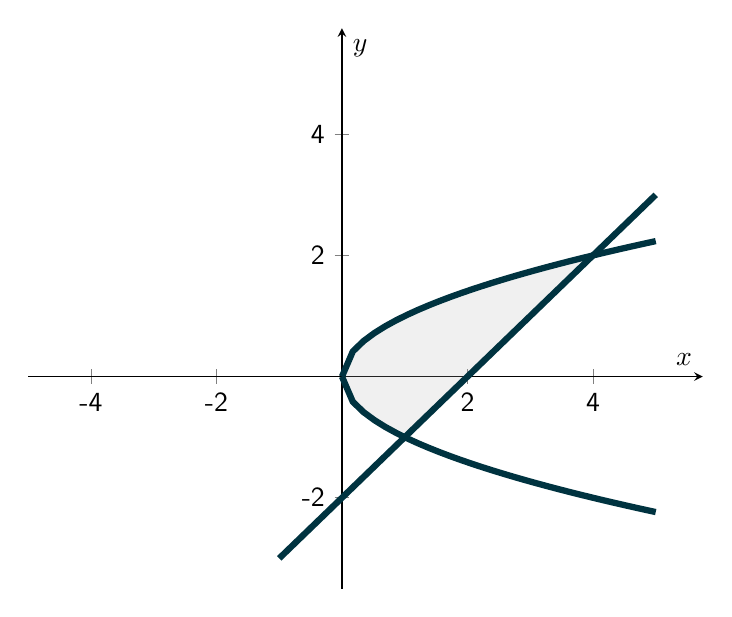
\begin{tikzpicture}[scale=1.25]
            \begin{axis}[
            axis lines = middle, very thick,
            xlabel = {$x$},
            ylabel = {$y$},
            xmin=-5, xmax=5.75,
            ymin=-3.5, ymax=5.75,
            xtick={-4,-2,0,2,4},
            xticklabels={-4,-2,0,2,4},
            ytick={-2,0,2,4},
            yticklabels={-2,0,2,4}        
            ]
            % Curves
            \addplot [name path = A,-,domain = 0:5, line width=0.8mm,DarkBlue,samples = 30] {sqrt(x)} ;
            \addplot [name path = B,-,domain = 0:5, line width=0.8mm,DarkBlue,samples = 30] {-sqrt(x)} ;
            \addplot [name path = C, line width=0.8mm, samples=4, smooth,domain=0:5, DarkBlue] coordinates {(-1,-3)(5,3)};
            % Fill area between paths
            \addplot [black!30, opacity=0.2] fill between [of = A and B, soft clip={domain=0:1}];
            \addplot [black!30, opacity=0.2] fill between [of = A and C, soft clip={domain=1:4}];
            \end{axis}
        \end{tikzpicture}    
    \end{center}   
        
    Thus
    \begin{align}
        \bar y &= \frac{M_x}M = \frac1M \int_{-1}^{2}\int_{y^2}^{y+2} 12y \, dx \, dy
    \end{align} 
    Thus
    \begin{align}
        a &= -1 \\
        b &= 2 \\
        c&= y^2 \\
        d&= y+2 \\
        f(x,y) &= \delta y = 12y
    \end{align}
    }
   \else

   \fi
    
\fi

\ifnum \Version=7
% SHORT SPHERICAL AND CYLINDRICAL EXERCISE
\part Point $P$ has rectangular (Cartesian) coordinates $(x,y,z) = (-6,0,8)$ in $\mathbb R^3$. In cylindrical coordinates, the point is $(r,\theta,z)$, and in spherical coordinates the point is $(\rho, \phi, \theta)$. Where $r=\framebox{\strut\hspace{1cm}}$, $\theta=\framebox{\strut\hspace{2cm}}$, $z=\framebox{\strut\hspace{1cm}}$, $\rho=\framebox{\strut\hspace{2cm}}$, and $\phi=\framebox{\strut\hspace{3cm}}$. 

    \ifnum \Solutions=1 {\color{DarkBlue} \textit{Solutions:} To convert to cylindrical we can use the equation $r^2 = x^2 + y^2$. 
    \begin{align}
        r^2 &= x^2 + y^2 = (-6)^2 + 0^2 = 36 \ \Rightarrow \ r = 6
    \end{align}
    To determine $\theta$ we can use $\tan\theta = y/x$. 
    \begin{align}
        \tan \theta &= \frac{y}{x} = \frac{0}{-6} = 0  \\
        \theta &= \arctan 0 
    \end{align} 
    The point in cylindrical is: 
    \begin{align}
        (r,\theta,z) &= (6,\pi,8) \\
        r &= 6 \\
        \theta &= \pi \\
        z &= 8
    \end{align}
    In spherical, we can start by obtaining $\rho$. 
    \begin{align}
        \rho^2 &= x^2+y^2+z^2\\
        \rho^2 &= (-6)^2 + 0^2 + 8^2 = 36+64 = 100 \\
        \rho &= 10
    \end{align}
    To obtain $\phi$ we can use the equation that relates $x$ to spherical. Using the expression for $x$, and the values that we already have for $x$, $\rho$ and $\theta$:
    \begin{align}
        x &= \rho \sin\phi \cos\theta \\
        -6 &= 10\sin\phi \cos(\pi) \\
        \sin\phi &= \frac{-6}{10 \cos(\pi)}  = \frac{6}{10}\\
        \phi &= \arcsin (6/10)
    \end{align}
    Our coordinates in spherical are
    \begin{align}
        \rho &= 10\\
        \phi &= \arcsin (6/10)\\
        \theta &= \pi
    \end{align}
    Note the following.
    \begin{itemize}
        \item We can, for this exercise, leave un-evaluated trig functions in the answer, because the question didn't specify that you should simplify your answer as much as possible. So it would be ok to leave your answer for $\theta$ as $\arctan 0$ or $\tan^{-1} 0$. 
        \item Our particular textbook uses the convention $(\rho, \phi, \theta)$, not $(\rho, \theta,\phi)$.
    \end{itemize}
    } 
    \else
      
    \fi
    
\fi





\ifnum \Version=8
% SHORT SPHERICAL AND CYLINDRICAL EXERCISE
\part Point $P$ has rectangular (Cartesian) coordinates $(x,y,z) = (4,4,7)$ in $\mathbb R^3$. In cylindrical coordinates, the point is $(r,\theta,z)$, and in spherical coordinates the point is $(\rho, \phi, \theta)$. Where $r=\framebox{\strut\hspace{1cm}}$, $\theta=\framebox{\strut\hspace{2cm}}$, $z=\framebox{\strut\hspace{1cm}}$, $\rho=\framebox{\strut\hspace{2cm}}$, and $\phi=\framebox{\strut\hspace{3cm}}$. 

    \ifnum \Solutions=1 {\color{DarkBlue} \textit{Solutions:} To convert to cylindrical we can use the equation $r^2 = x^2 + y^2$. 
    \begin{align}
        r^2 &= x^2 + y^2 = (4)^2 + 4^2 = 32 \ \Rightarrow \ r = \sqrt{32} = 4\sqrt2
    \end{align}
    It isn't necesssary to simplify to $4\sqrt2$. Then to determine $\theta$ we can use $\tan\theta = y/x$. 
    \begin{align}
        \tan \theta &= \frac{y}{x} = \frac{4}{4} = 1  \\
        \theta &= \arctan \pi/4
    \end{align} 
    The point in cylindrical is: 
    \begin{align}
        (r,\theta,z) &= (4\sqrt2,\pi/4,7) \\
        r &= 4\sqrt2 \\
        \theta &= \pi/4 \\
        z &= 7
    \end{align}
    In spherical, we can start by obtaining $\rho$. 
    \begin{align}
        \rho^2 &= x^2+y^2+z^2\\
        \rho^2 &= (4)^2 + 4^2 + 7^2 = 16+16+49 = 32+49 = 81 \\
        \rho &= 9
    \end{align}
    To obtain $\phi$ we can use the equation that relates $x$ to spherical. Using the expression for $x$, and the values that we already have for $x$, $\rho$ and $\theta$:
    \begin{align}
        x &= \rho \sin\phi \cos\theta \\
        4 &= 9\sin\phi \cos(\pi/4) \\
        \sin\phi &= \frac{4}{9 \cos(\pi/4)}  = \frac{4\sqrt2}{9}\\
        \phi &= \arcsin \left(\frac{4\sqrt2}{9}\right)
    \end{align}
    Note for $\phi$ we can also use:
    \begin{align}
        y &= \rho \sin\phi \sin\theta \\
        4 &= 9\sin\phi \sin(\pi/4) \\
        \sin\phi &= \frac{4}{9 \sin(\pi/4)}  = \frac{4\sqrt2}{9}\\
        \phi &= \arcsin \left(\frac{4\sqrt2}{9}\right)
    \end{align}    
    And we can also use:
    \begin{align}
        z &= \rho \cos\phi  \\
        7 &= 9\cos\phi  \\
        \sin\phi &= \frac{4}{9 \sin(\pi/4)}  = \frac{4\sqrt2}{9}\\
        \phi &= \arccos \left(\frac{7}{9}\right)
    \end{align}      
    Our coordinates in spherical are
    \begin{align}
        \rho &= 9\\
        \phi &= \arcsin \left(\frac{4\sqrt2}{9}\right), \ \textbf{or} \ \phi = \arccos(7/9)\\
        \theta &= \pi/4
    \end{align}
    Note the following.
    \begin{itemize}
        \item We can, for this exercise, leave un-evaluated trig functions in the answer, because the question didn't specify that you should simplify your answer as much as possible. So it would be ok to leave your answer for $\theta$ as $\arctan 1$ or $\tan^{-1} 1$. 
        \item Our particular textbook uses the convention $(\rho, \phi, \theta)$, not $(\rho, \theta,\phi)$.
    \end{itemize}
    } 
    \else
      
    \fi
    
\fi





% 15.6
% CENTROID Y-COORDINATE PARABOLA AND LINE
\ifnum \Version=9
    \part A thin plate with density $\delta=12$ is bounded in the $xy-$plane by $y=3-x^2$ and $y=1-x$. The plate has mass $M$. The $y-$coordinate of the centroid is $\bar y = M_x/M$, where $\displaystyle M_x = \int_A^B \int_C^D f(x,y) \, dy \, dx$,  and $A=\framebox{\strut\hspace{1cm}}$, $B=\framebox{\strut\hspace{1cm}}$, $C=\framebox{\strut\hspace{3cm}}$, $D=\framebox{\strut\hspace{3cm}}$, and $f(x,y) = \framebox{\strut\hspace{3cm}}$. 
    
    \ifnum \Solutions=1 
    {\color{DarkBlue}
    The region is bounded by 
    $$1-x \le y \le 3-x^2$$
    The given curves intersect when 
    \begin{align}
        1-x &= 3-x^2\\
        0 &= x^2-x-2 \\
        &= (x-2)(x+1)
    \end{align}
    The curves intersect at $x=-1,2$. Using $y=1-x$, the intersection points are $(-1,2)$ and $(2,-1)$. The region is shown below. 
    \begin{center}  
        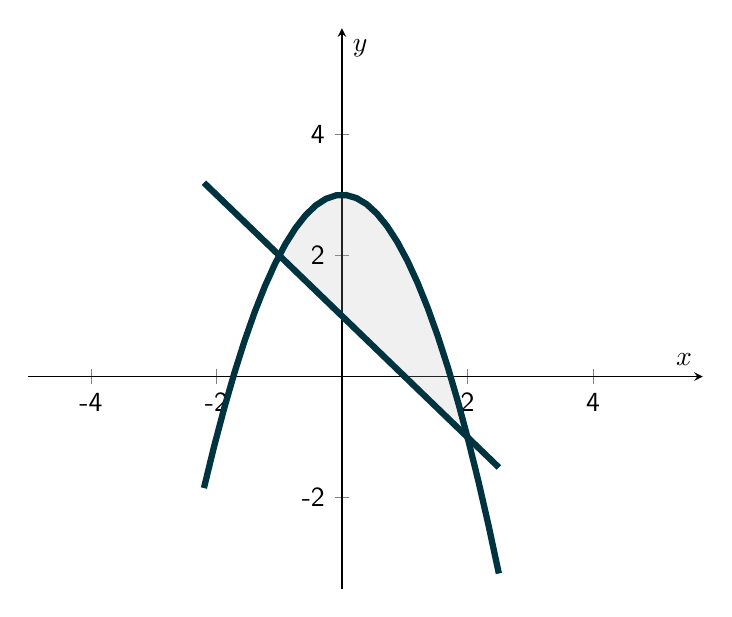
\begin{tikzpicture}[scale=1.25]
            \begin{axis}[
            axis lines = middle, very thick,
            xlabel = {$x$},
            ylabel = {$y$},
            xmin=-5, xmax=5.75,
            ymin=-3.5, ymax=5.75,
            xtick={-4,-2,0,2,4},
            xticklabels={-4,-2,0,2,4},
            ytick={-2,0,2,4},
            yticklabels={-2,0,2,4}        
            ]
            % Curves
            \addplot [name path = A,-,domain = -2.2:2.5, line width=0.8mm,DarkBlue,samples = 30] {3-x^2} ;
            \addplot [name path = C,-,domain = -2.2:2.5, line width=0.8mm,DarkBlue,samples = 4] {1-x} ;
            % Fill area between paths
            \addplot [black!30, opacity=0.2] fill between [of = A and C, soft clip={domain=-1:2}];
            \end{axis}
        \end{tikzpicture}    
    \end{center}   
        
    Thus
    \begin{align}
        \bar y &= \frac{M_x}M = \frac1M \int_{-1}^{2}\int_{1-x}^{3-x^2} 12y \, dy \, dx
    \end{align} 
    Thus
    \begin{align}
        A &= -1 \\
        B &= 2 \\
        C&= 1-x \\
        D&= 3-x^2 \\
        f(x,y) &= \delta y = 12y
    \end{align}
    }
   \else

   \fi
    
\fi
   
    % 13.3 and 13.4
% unit tangent vectors
% arc length
% curvature
% osculating circle
% unit normal

\ifnum \Version=1

\part The unit tangent vector for a curve $\mathbf r(t)$ is $\mathbf T(t) = \langle 0, \cos t, \sin t \rangle$. The unit normal vector is $\mathbf  N = \langle f(t), g(t), g(t) \rangle$, where $f(t) = \framebox{\strut\hspace{2cm}}$, $g(t) = \framebox{\strut\hspace{2cm}}$, $h(t) =\framebox{\strut\hspace{2cm}}$. 

\ifnum \Solutions=1 {\color{DarkBlue} \textit{Answer:} \textit{Solutions:} The normal vector is

\begin{align}
    \mathbf N &= \frac{d\mathbf T/dt}{|d\mathbf T/dt|} 
\end{align}
And
\begin{align}
    \mathbf T'(t) &= \langle 0,-\sin t, \cos t \rangle \\
    |\mathbf T'(t) | &= \sqrt{ 0 +(-\sin t)^2 + (\cos t)^2} =1\\
    \mathbf N &= \frac{d\mathbf T/dt}{|d\mathbf T/dt|} = \langle 0, - \sin(t),  \cos(t) \rangle
\end{align}
} 
\else
\fi        
\fi

\ifnum \Version=2

\part The velocity vector of an object moving on the curve $\mathbf r(t)$ is $\mathbf v(t) = \langle 4\cos (2t), 4\sin (2t) , 3 \rangle$ for $t>0$. The speed of the object for $t>0$ is $s(t) = |\mathbf v | = \framebox{\strut\hspace{1cm}}$. The unit tangent vector for $t>0$ is $\mathbf T = \langle f(t), g(t) , h(t) \rangle$, where $f(t) = \framebox{\strut\hspace{1.5cm}}$, $g(t) = \framebox{\strut\hspace{1.5cm}}$, $h = \framebox{\strut\hspace{1cm}}$. The curvature is $\kappa = \framebox{\strut\hspace{1cm}}$. 

\ifnum \Solutions=1 {\color{DarkBlue} \textit{Answer:} \textit{Solutions:} The speed is the magnitude of the given velocity vector and is
\begin{align}
    s &= |\mathbf v | =  \sqrt{(4\cos2t)^2 + (4\sin2t)^2 + 3^2 } = \sqrt{4^2 (\cos ^2 2 t + \sin^2 2t) + 3^2} = \sqrt{16 + 9} = 5
\end{align}
The unit tangent vector is 
\begin{align}
    \mathbf T &= \frac{\mathbf v}{|\mathbf v|} = \langle \frac{4}{5}\cos(2 t) , \frac 45 \sin (2t), \frac35 \rangle
\end{align}
For curvature we also need
\begin{align}
    \frac{d\mathbf T}{dt } &= \langle -\frac85 \sin 2t, \frac85 \cos 2t,0 \rangle \\
    \left | \frac{d\mathbf T}{dt } \right| &= \sqrt{ \left(-\frac85\sin 2t\right)^2 +   \left(\frac85 \cos 2 t\right)^2 } = \frac85
\end{align}
The curvature is
\begin{align}
    \kappa = \frac{1}{|\mathbf v |}\left| \frac{d\mathbf T}{dt}\right| = \frac{1}{5} \cdot \frac{8}{5} = \frac{8}{25}
\end{align}
} 
\else
\fi        
\fi


\ifnum \Version=3

\part A plane curve $\mathbf r(t)$ has curvature $\kappa = \frac{1}{8}$ at $\mathbf r(t_0) = \langle 15, 2 \rangle$, and the unit normal vector at $t=t_0$ is $\mathbf  N = \mathbf j = \langle 0, 1 \rangle$. The equation of the osculating circle at $t=t_0$ is \framebox{\strut\hspace{3.5cm}}.

\ifnum \Solutions=1 {\color{DarkBlue} \textit{Answer:} \textit{Solutions:} Recall that The circle of curvature, or osculating circle, at a point $P$ on a plane curve where $\kappa \ne 0$ is the circle in the plane of the curve that

\begin{enumerate}
    \item is tangent to the curve at P (has the same tangent line the curve has)
    \item has the same curvature the curve has at P
    \item lies toward the concave or inner side of the curve
\end{enumerate}
The \textbf{radius of curvature} of the curve at P is the radius of the circle of curvature, which is $\frac{1}{\kappa}$. So to obtain the radius, we calculate $\kappa$ and take the reciprocal. The \textbf{center} of the osculating circle of the curve at P lies on the inner side of the curve, and the unit normal points in the direction of the inner side of the planar curve. 

So for this problem we have a circle with radius $1/\kappa = 8$, and whose centre is 8 units away from the point $(15,2)$ in the direction of $\mathbf N$. The circle has equation
$$(x-15)^2 + (y-10)^2 = 8^2$$
} 
\else
  
\fi        
\fi




\ifnum \Version=4

\part The velocity vector for an object moving on the curve $\mathbf r(t)$ is $\mathbf v(t) = \langle t\cos t, t\sin t \rangle$. The speed of the object for $t>0$ is $s(t) = \framebox{\strut\hspace{1cm}}$. The unit tangent vector for $t>0$ is $\mathbf T = \langle f(t), g(t) \rangle$, where $f(t) = \framebox{\strut\hspace{2cm}}$, $g(t) = \framebox{\strut\hspace{2cm}}$. 

\ifnum \Solutions=1 {\color{DarkBlue} \textit{Answer:} \textit{Solutions:} The speed is the magnitude of the velocity vector and is
\begin{align}
    s &= |\mathbf v | = \sqrt{(t\cos t)^2 + (t\sin t)^2 } = \sqrt{t^2 (\cos ^2 t + \sin^2 t)} = |t|
\end{align}
But we are told that $t>0$ so we can use $|t| = t$. The unit tangent vector is 
\begin{align}
    \mathbf T &= \frac{\mathbf v}{|\mathbf v|} = \langle \cos t, \sin t \rangle
\end{align}
} 
\else
\fi        
\fi

\ifnum \Version=5

\part A plane curve $\mathbf r(t)$ has curvature $\kappa = \frac{1}{4}$ at the point $\mathbf r(t_0) = 3\mathbf i + 5\mathbf j$, and the unit normal vector at $t_0$ is $\mathbf  N = \mathbf i = \langle1,0\rangle$. The equation of the osculating circle at $t=t_0$ is \framebox{\strut\hspace{3.5cm}}.

\ifnum \Solutions=1 {\color{DarkBlue} \textit{Answer:} \textit{Solutions:} Recall that The circle of curvature, or osculating circle, at a point $P$ on a plane curve where $\kappa \ne 0$ is the circle in the plane of the curve that

\begin{enumerate}
    \item is tangent to the curve at P (has the same tangent line the curve has)
    \item has the same curvature the curve has at P
    \item lies toward the concave or inner side of the curve
\end{enumerate}
The \textbf{radius of curvature} of the curve at P is the radius of the circle of curvature, which is $\frac{1}{\kappa}$. So to obtain the radius, we calculate $\kappa$ and take the reciprocal. The \textbf{center} of the osculating circle of the curve at P lies on the inner side of the curve, and the unit normal points in the direction of the inner side of the planar curve. 

So for this problem we have a circle with radius $1/\kappa = 4$, and whose centre is 4 units away from the point $(3,5)$ in the direction of $\mathbf N$. The circle has equation
$$(x-7)^2 + (y-5)^2 = 4^2$$
} 
\else
  
\fi        
\fi


\ifnum \Version=6

\part The velocity vector for an object moving on the curve $\mathbf r(t)$ is $\mathbf v(t) = \langle 4t\cos t, 4t\sin t \rangle$ for $t>0$. The speed of the object for $t>0$ is $s(t)  = |\mathbf v | = \framebox{\strut\hspace{1cm}}$. The unit tangent vector for $t>0$ is $\mathbf T = \langle f(t), g(t) \rangle$, where $f(t) = \framebox{\strut\hspace{1.5cm}}$, $g(t) = \framebox{\strut\hspace{1.5cm}}$. The curvature is $\kappa = \framebox{\strut\hspace{1cm}}$. 

\ifnum \Solutions=1 {\color{DarkBlue} \textit{Answer:} \textit{Solutions:} The speed is the magnitude of the given velocity vector and is
\begin{align}
    s &= |\mathbf v | =  \sqrt{(4t\cos t)^2 + (4t\sin t)^2 } = \sqrt{4^2t^2 (\cos ^2 t + \sin^2 t)} = 4|t|
\end{align}
But we are told that $t>0$ so we can assume $|t| = t$. The unit tangent vector is 
\begin{align}
    \mathbf T &= \frac{\mathbf v}{|\mathbf v|} = \langle \cos t, \sin t \rangle
\end{align}
We need
\begin{align}
    \frac{d\mathbf T}{dt } &= \langle -\sin t, \cos t \rangle \\
    \left | \frac{d\mathbf T}{dt } \right| &= \sqrt{ (-\sin t)^2 +   \cos^2 t } = 1
\end{align}
The curvature is
\begin{align}
    \kappa = \frac{1}{|\mathbf v |}\left| \frac{d\mathbf T}{dt}\right| = \frac{1}{4t} 
\end{align}
} 
\else
\fi        
\fi



\ifnum \Version=7

\part The velocity vector of an object moving on the curve $\mathbf r(t)$ is $\mathbf v(t) = \langle 3\cos (2t), 3\sin (2t) \rangle$ for $t>0$. The speed of the object for $t>0$ is $s(t) = |\mathbf v | = \framebox{\strut\hspace{1.5cm}}$. The unit tangent vector for $t>0$ is $\mathbf T = \langle f(t), g(t)  \rangle$, where $f(t) = \framebox{\strut\hspace{2cm}}$, and $g(t) = \framebox{\strut\hspace{2cm}}$.  The curvature for $t>0$ is \framebox{\strut\hspace{1.5cm}}. 

\ifnum \Solutions=1 {\color{DarkBlue} \textit{Answer:} \textit{Solutions:} The speed is the magnitude of the given velocity vector and is
\begin{align}
    s &= |\mathbf v | =  \sqrt{(3\cos t)^2 + (3\sin t)^2  } = \sqrt{3^2 (\cos ^2 t + \sin^2 t) + 3^2} = \sqrt{ 9} = 3
\end{align}
The unit tangent vector is 
\begin{align}
    \mathbf T &= \frac{\mathbf v}{|\mathbf v|} 
    = \langle \frac{3}{3}\cos(2 t) , \frac 33 \sin (2t) \rangle 
    = \langle \cos(2 t) ,  \sin (2t) \rangle
\end{align}
For curvature we also need
\begin{align}
    \frac{d\mathbf T}{dt } &= \langle -2 \sin 2t, 2 \cos 2t\rangle \\
    \left | \frac{d\mathbf T}{dt } \right| &= \sqrt{ \left(-2\sin 2t\right)^2 +   \left(2 \cos 2 t\right)^2 } = 2
\end{align}
The curvature is
\begin{align}
    \kappa = \frac{1}{|\mathbf v |}\left| \frac{d\mathbf T}{dt}\right| = \frac{1}{3} \cdot 2 = \frac{2}{3}
\end{align}
} 
\else
\fi        
\fi


\ifnum \Version=8

\part A plane curve $\mathbf r(t)$ has curvature $\kappa = \frac{1}{4}$ at $\mathbf r(t_0) = \langle 5, 3 \rangle$, and the unit normal vector at $t=t_0$ is $\mathbf  N = \mathbf j = \langle 0, 1 \rangle$. The equation of the osculating circle at $t=t_0$ is \framebox{\strut\hspace{3.5cm}}.

\ifnum \Solutions=1 {\color{DarkBlue} \textit{Answer:} \textit{Solutions:} Recall that The circle of curvature, or osculating circle, at a point $P$ on a plane curve where $\kappa \ne 0$ is the circle in the plane of the curve that

\begin{enumerate}
    \item is tangent to the curve at P (has the same tangent line the curve has)
    \item has the same curvature the curve has at P
    \item lies toward the concave or inner side of the curve
\end{enumerate}
The \textbf{radius of curvature} of the curve at P is the radius of the circle of curvature, which is $\frac{1}{\kappa}$. So to obtain the radius, we calculate $\kappa$ and take the reciprocal. The \textbf{center} of the osculating circle of the curve at P lies on the inner side of the curve, and the unit normal points in the direction of the inner side of the planar curve. 

So for this problem we have a circle with radius $1/\kappa = 4$, and whose centre is 4 units away from the point $(5,3)$ in the direction of $\mathbf N$. The circle has equation
$$(x-5)^2 + (y-7)^2 = 4^2$$
} 
\else
  
\fi        
\fi






\ifnum \Version=9

\part The velocity vector of an object moving on the curve $\mathbf r(t)$ is $\mathbf v(t) = \langle t, 3 \rangle$ for $t>0$. The speed of the object at $t=2$ is $s(2) = |\mathbf v(2) | = \framebox{\strut\hspace{1.75cm}}$. The unit tangent vector at $t=2$ is $\mathbf T(2) = \langle c_1 ,c_2  \rangle$, where $c_1 = \framebox{\strut\hspace{1.75cm}}$, $c_2 = \framebox{\strut\hspace{1.75cm}}$. The curvature is $\framebox{\strut\hspace{1.75cm}}$. 

\ifnum \Solutions=1 {\color{DarkBlue} \textit{Answer:} \textit{Solutions:} The speed is the magnitude of the given velocity vector and is
\begin{align}
    s &= |\mathbf v | =  \sqrt{( t)^2 + (3)^2  } = \sqrt{t^2+9}\\
    s(2) &= \sqrt{2^2+9} = \sqrt{13}
\end{align}
We also need the unit tangent vector at $t=2$. 
\begin{align}
    \mathbf T (t) &= \frac{\mathbf v}{|\mathbf v|} = \frac{t\mathbf i + 3\mathbf j}{\sqrt{t^2+9}} \\
    \mathbf T (2) &= \frac{2\mathbf i + 3\mathbf j}{\sqrt{2^2+9}}  
    = \langle \frac{2}{\sqrt{13}} , \frac {3}{\sqrt{13}}  \rangle \\
    c_1 &= \frac{2}{\sqrt{13}}\\
    c_2 &= \frac{3}{\sqrt{13}}
\end{align}
The curvature is zero because the motion is along a straight line. 
\begin{align}
    \kappa = 0
\end{align}
} 
\else
\fi        
\fi

\ifnum \Version=10

\part A plane curve $\mathbf r(t)$ has curvature $\kappa = \frac{1}{10}$ at $\mathbf r(t_0) = \langle 5, 0 \rangle$, and the unit normal vector at $t=t_0$ is $\mathbf  N = \mathbf j = \langle 0, 1 \rangle$. The equation of the osculating circle at $t=t_0$ is \framebox{\strut\hspace{3.5cm}}.

\ifnum \Solutions=1 {\color{DarkBlue} \textit{Answer:} \textit{Solutions:} Recall that The circle of curvature, or osculating circle, at a point $P$ on a plane curve where $\kappa \ne 0$ is the circle in the plane of the curve that

\begin{enumerate}
    \item is tangent to the curve at P (has the same tangent line the curve has)
    \item has the same curvature the curve has at P
    \item lies toward the concave or inner side of the curve
\end{enumerate}
The \textbf{radius of curvature} of the curve at P is the radius of the circle of curvature, which is $\frac{1}{\kappa}$. So to obtain the radius, we calculate $\kappa$ and take the reciprocal. The \textbf{center} of the osculating circle of the curve at P lies on the inner side of the curve, and the unit normal points in the direction of the inner side of the planar curve. 

So for this problem we have a circle with radius $1/\kappa = 10$, and whose centre is 10 units away from the point $(5,0)$ in the direction of $\mathbf N$. The circle has equation
$$(x-5)^2 + (y-10)^2 = 10^2$$
} 
\else
  
\fi        
\fi
   
\end{parts}

\newpage \question[0.25] \ID
% CHANGE OF VARIABLE (15.8)
% OR APPLICATION (15.6)
% OR TRIPLE CARTESIAN (15.5) 

\ifnum \Version=1
% CENTROID
% BASED ON THOMAS EXERCISES, 15.6 #1
% SUFFICIENT FOR A PRACTICE EXAM
\question[6] A thin plate of density $\delta(x,y) = 12x$ is bounded by the lines $x = 0, y = x$, and the parabola $y = x^2-6$ in the first quadrant. 
\begin{parts} 
    \part Determine the mass of the plate, $M$. Please show your work. 
    \ifnum \Solutions=1 
    {\color{DarkBlue} \textit{Solutions:}
    Curves intersect when $$x = x^2-6 \quad \Rightarrow \quad 0 = x^2 - x - 6 = (x-3)(x+2)$$
    Or $x=3, -2$. We can ignore $x=-2$ because the region is the first quadrant. Curves intersect at the point $(3,3)$, and 
    \begin{align}
        0 \le y \le 3, \quad y \le x \le \sqrt{y+6}
    \end{align}
    The mass is
    \begin{align}
        M &= \int_0^3 \int_y^{\sqrt{y+6}} \delta \, dx \, dy \\
        &= \int_0^3 \int_y^{\sqrt{y+6}} 12x \, dx \, dy \\
        &= \int_0^3  \left. 6x^2 \right|_{x=y}^{x=\sqrt{y+6}} \, dy \\
        &= \int_0^3 6(y + 6 - y^2) \, dy \\
        &= \int_0^3 6y + 36 - 6y^2 \, dy \\
        &= \left. (3y^2 + 36y - 2y^3 ) \right|_0^3 \, dy \\
        &= 27 + 108 - 54 \\
        &= 81
    \end{align}
    }
    \else 
    \vspace{16cm}
    \fi
    \part Use your results from the previous part to set up an integral that can be used to determine the $x-$coordinate of the center of mass of the plate. You do not need to evaluate your integral. 
    \ifnum \Solutions=1 {\color{DarkBlue} \textit{Solutions:} the $x-$coordinate of the center of mass, $\bar x$, is
    \begin{align}
    \bar x &= \frac{M_y}{M} = \frac{1}{81} \int_0^3 \int_y^{\sqrt{y+6}} 12x^2 \, dx \, dy 
    \end{align}
    } 
    \else
      
    \fi
    \end{parts} 
\fi
    





\ifnum \Version=2
% LONGISH CHANGE OF VARIABLE
% VERBATUM FROM SPRING 2022 QUIZ
% hand written solution only
% SUFFICIENT FOR A PRACTICE EXAM
\question[6] Consider the double integral

$$I=\iint_R \frac{x+2y}{2y-x} dA$$

where $R$ is the parallelogram with vertices $(-3,1), (-1,0), (-1,2), (1,1)$. Our goal is to determine the area of the parallelogram using the transform below. 
$$u=x+2y, \qquad v = -x +2y$$ 
Please show your work for the following. 
\begin{parts} 
    \part Use the given transform to calculate the Jacobian of the transform, $J = \partial x(u,v)/\partial y(u,v)$. 
    \ifnum \Solutions=1 
    \else 
    \vspace{8 cm}
    \fi
    \part Use your results from Part (a) and the given transform to transform the double integral. You do not need to evaluate your integral. 
\end{parts} 

\ifnum \Solutions=1 {\color{DarkBlue} \textit{Solutions:} the integral after the transform is $$\displaystyle \frac14 \int_1^5\int_{-1}^3 \frac uv \, du \, dv$$
A screen capture of a hand-written solution from a previous offer of MATH 2551 is below. 
    \begin{figure}[h]
    \centering
    \includegraphics[width=16cm]{202302/Exam3/Images/ImgE3.OR.06.png}
    \end{figure}  
    
    } 
   \else
      
   \fi
    
\fi

\ifnum \Version=3
% CENTROID
% BASED ON THOMAS EXERCISES, 15.6 #1
% SUFFICIENT FOR A PRACTICE EXAM
\question[6] A thin plate with density $\delta(x,y) = 24y$ is bounded by the lines $x = 0, x=2y$, and the parabola $x=y^2$ in the first quadrant. 
\begin{parts} 
    \part Determine the mass of the plate, $M$. Please show your work. 
    
    \ifnum \Solutions=1 
    {\color{DarkBlue} \textit{Solutions:}
    Curves intersect when $$2y = y^2 \quad \Rightarrow \quad 0 = y^2-2y = y(y-2)$$
    Or $y=0,2$. Curves intersect at the points $(0,0)$, $(4,2)$. 
    The mass is
    \begin{align}
        M = \int_0^4 \int_{x/2}^{\sqrt{x}} \delta \, dy \, dx 
        &= \int_0^4 \int_{x/2}^{\sqrt{x}} 24y \, dy \, dx \\
        &= \int_0^4  \left. 12y^2 \right|_{y=x/2}^{y=\sqrt{x}} \, dx \\
        &= 12 \int_0^4 (x-\frac{x^2}{4}) \, dx \\
        &= 12 \left. (\frac{x^2}{2} - \frac{x^3}{12} ) \right|_0^4 \, dy \\
        &= 12 (\frac{16}{2} - \frac{64}{12}) \\
        &= 96 - 64\\
        &= 32
    \end{align}
    \textbf{An Alternate Solution}\\
    Another way to approach this problem is to use the integration order $dx\,dy$. In this case the double integral becomes
    \begin{align}
        M = \int_0^2 \int_{y^2}^{2y} \delta \, dx \, dy
        &= \int_0^2 \int_{y^2}^{2y} 24y \, dx \, dy \\
        &= 24\int_0^2  \left. yx \right|_{x=y^2}^{x=2y} \, dy \\
        &= 24 \int_0^2 (2y^2 - y^3) \, dy \\
        &= 24 \left. (\frac{2y^3}{3} - \frac{y^4}{4} ) \right|_0^2 \, dy \\
        &= 24 (\frac{16}{3} - \frac{16}{4}) \\
        &= \frac{24\cdot16}{3} - 24\cdot 4 \\
        &= 8\cdot16 - 96 \\
        &= 128 - 96 \\
        &= 32
    \end{align}    
    }
    \else 
    \vspace{14cm}
    \fi
    \part Use your results from the previous part to set up an integral that can be used to determine the $x-$coordinate of the center of mass of the plate. You do not need to evaluate your integral. 
    \ifnum \Solutions=1 {\color{DarkBlue} \textit{Solutions:} the $x-$coordinate of the center of mass, $\bar x$, is
    \begin{align}
    \bar x &= \frac{M_y}{M} = \frac{1}{32} \int_0^4 \int_{x/2}^{\sqrt{x}} 24xy \, dy \, dx
    \end{align}
    \textbf{An Alternate Solution}\\    
    It is also ok to use the integration order $dx\,dy$. In this case the double integral becomes
    \begin{align}
    \bar x &= \frac{M_y}{M} = \frac{1}{32} \int_0^2 \int_{y^2}^{2y} 24xy \, dx \, dy 
    \end{align}
    } 
    \else
      
    \fi
    \end{parts} 
\fi

\ifnum \Version=4
% VERSION B
% LONG CHANGE OF VARIABLE
% BASED ON AN EXAMPLE FROM THOMAS
% SECTION 15.8 FROM THOMAS
\question[6] Consider the double integral

$$I= 9 \iint_R (y-2x)^2 \sqrt{x+y} \, dA$$

where $R$ is the region in the first quadrant bounded by the lines $x=0$, $y=0$, and $y=1-x$. Our goal is to determine the area of $R$ using the transform below. 
$$u=x+y, \qquad v = y-2x$$ 
Please show your work for the following. 
\begin{parts} 
    \part Use the given transform to calculate the Jacobian of the transform, $J = \partial x(u,v)/\partial y(u,v)$. 
    \ifnum \Solutions=1 {\color{DarkBlue} \textit{Solutions:} Solving for $x$ and $y$ using an augmented matrix,
    \begin{align}
        \begin{pmatrix} 1 & 1 & u \\-2 & 1 & v\end{pmatrix} 
        \sim \begin{pmatrix} 1 & 1 & u \\0 & 3 & 2u+v\end{pmatrix} 
        \sim \begin{pmatrix} 1 & 0 & u/3 - v/3 \\0 & 1 & 2u/3+v/3 \end{pmatrix} 
    \end{align}
    Thus
    \begin{align}
        x &= \frac13(u-v), \ y = \frac13(2u+v) \\
        J(u,v) & = \begin{vmatrix} \DXDU & \DXDV \\[8pt] \DYDU & \DYDV \end{vmatrix} = \begin{vmatrix} 1/3 & -1/3 \\ 2/3 & 1/3 \end{vmatrix} = 1/9 + 2/9 = 1/3
    \end{align}
    }
    \else 
    \vspace{8 cm}
    \fi
    \part Use the given transform and your results from Part (a) to convert the double integral into a double integral over a region in the $uv-$plane. You do not need to evaluate your integral. 
    \ifnum \Solutions=1 {\color{DarkBlue} \textit{Solutions:} Converting each of the boundaries in the $xy-$plane into the $uv-$plane we obtain
        \begin{align}
            x+y &= 1 \quad \Rightarrow \quad \frac13(u-v) + \frac13(2u+v) = 1 &&\Rightarrow \quad u = 1\\
            x&=0 \quad \Rightarrow \quad \frac13(u-v) = 0 &&\Rightarrow \quad v = u\\
            y&= 0 \quad \Rightarrow \quad \frac13(2u+v) = 0 &&\Rightarrow \quad v = -2u
        \end{align}
        The region is described by either of the following relations:
        \begin{align}
            S_1: & \quad 0 \le u \le 1, \quad -2u \le v \le u \\
            S_2: & \quad -2 \le v \le 0, \quad -v/2 \le u \le 1, \ \text{and } 0 \le v \le 1, \quad v \le u \le 1
        \end{align}
        The first set of inequalities requires only a single double integral, but it is ok to set up two double integrals. If using $S_1$, we use $dv\,du$ and obtain
        \begin{align}
            I= 9 \iint_R (y-2x)^2 \sqrt{x+y} \, dA = 9 \int_0^1 \int_{-2u}^u v^2u^{1/2} \frac13 \,dv\,du
        \end{align}
        If using $S_2$, we use $du\,dv$ and obtain
        \begin{align}
            I= 9 \iint_R (y-2x)^2 \sqrt{x+y} \, dA 
            = 9 \int_{-2}^0 \int_{-v/2}^1 v^2u^{1/2} \frac13 \,du\,dv
            + 9 \int_{0}^1 \int_{v}^1 v^2u^{1/2} \frac13 \,du\,dv
        \end{align}        
        } 
       \else
          
       \fi
    \end{parts} 

    \fi



\ifnum \Version=5
    % USE FOR VERSION B
    % LONG CYLINDRICAL WITH APPLICATION TO MASS WITH VARYING DENSITY
    % FROM 15.8
    \question[6] An object $D$ lying in the first octant is bounded below by the $xy-$plane, above by the plane $z=3+4y$, and by the cylinder $x^2+y^2 = 4$. The density of the object at any point in $D$ is equal to the distance from the point to the $z$-axis.  Please show your work for the following.
    
    \begin{parts} 
    \part Use cylindrical coordinates to calculate the total of mass of the object, $M$. Please show your work. 
    
    \ifnum \Solutions=1 {\color{DarkBlue} The object is only in the first octant so $$0 \le \theta \le \pi/2$$ Using $\delta = \sqrt{x^2+y^2} = r$, the $z-$coordinate of the center of mass is computed using 
    \begin{align}
        M &= \iiint_D  \delta \, dV \\
        &= \int_0^{\pi/2} \int_0^2 \int_0^{3+4r\sin\theta}  \delta(r,\theta) \, r\, dz\,dr\,d\theta\\
        &= \int_0^{\pi/2} \int_0^2 \int_0^{3+4r\sin\theta}   r^2 \, dz\,dr\,d\theta\\
        &= \int_0^{\pi/2} \int_0^2    r^2 \, (3+4r\sin\theta) \,dr\,d\theta \\
        &= \int_0^{\pi/2} \int_0^2     \, (3r^2+4r^3\sin\theta) \,dr\,d\theta \\
        &= \int_0^{\pi/2}  \left. \, (r^3+r^4\sin\theta) \right|_{r=0}^{r=2} d\theta \\
        &= \int_0^{\pi/2}  (8 + 16\sin\theta) d\theta \\
        &=  \left. (8\theta - 16\cos\theta) \right|_0^{\pi/2} \\
        &=  (4\pi - 0) - (0 - 16) \\
        &= 4\pi + 16
    \end{align}
    
    } 
    \else
        \vspace{14cm}
    \fi
    
    \part Use your results from the previous part to set up a triple integral in cylindrical coordinates that can be used to determine the $z-$coordinate of the center of mass of the object. You do not need to evaluate your integral. 

    \ifnum \Solutions=1 {\color{DarkBlue} \textit{Solutions:} the $z-$coordinate of the center of mass, $\bar x$, is
    \begin{align}
    \bar z &= \frac{M_{xy}}{M} = \frac{1}{16\pi+16} \int_0^{\pi/2} \int_0^2 \int_0^{3+4r\sin\theta}  z \, \delta(r,\theta) \, r\, dz\,dr\,d\theta
    \end{align}
    } 
    \else
      
    \fi
    \end{parts} 
\fi


% TRANSFORM: SOLVE FOR X & Y, BOUNDARIES, EVALUATE, TRIANGLES
% VERSION A
\ifnum \Version=6
    \question[6] Consider the transform $u=x+y$ and $v=4x+5y$, and the integral $\displaystyle I = \iint_{R}  \,dxdy$. Region $R$ is the triangle in the $xy$-plane bounded by $x+y=0$, $4x+5y=0$, $6x+7y=4$. The transform maps $R$ to region $G$ in the $uv-$plane.  Please show your work for the following.

    \begin{enumerate}
        \item[a)] Solve the system, $u=x+y$ and $v=4x+5y$, for $x$ and $y$ in terms of $u$ and $v$.
            \ifnum \Solutions=1 {\color{DarkBlue} \\[12pt] 
            \textbf{Solutions:}
            We can use the expressions for $u$ and $v$ as an augmented matrix and row reduce. 
            \begin{align}
                \begin{pmatrix} 1 & 1 & u \\ 4 & 5 & v\end{pmatrix} 
                \sim \begin{pmatrix} 1 & 1 & u \\0 & 1 & v - 4u \end{pmatrix} 
                \sim \begin{pmatrix} 1 & 0 & 5u - v \\ 0 & 1 & v - 4u \end{pmatrix} 
            \end{align}
            Thus $x = 5u - v$, and $y = v - 4u$. 
            } 
            \else 
            \vspace{5cm}
            \fi
        \item[b)] Transform the boundaries of $R$ to the $uv-$plane. In other words, determine the boundaries of $G$ in terms of $u$ and $v$. 
            \ifnum \Solutions=1 {\color{DarkBlue} \\[12pt] 
            \textbf{Solutions:} the three lines are transformed below. 
            \begin{itemize}
                \item The line $x+y=0$ becomes $u=0$. 
                \item The line $4x+5y=0$ becomes $v=0$. 
                \item The line $6x+7y=4$ is: 
                \begin{align}
                    6x+7y &=4 \\
                    6\cdot(5u-v) + 7\cdot(v-4u) &= 4\\
                    30u -28u -6v+7v &=4 \\
                    v &= 4 -2u
                \end{align}
            \end{itemize}
            } 
        \else 
        \vspace{5cm}
        \fi        
            
        \item[c)] Use the given transformation and your results from parts (a) and (b) to set up a double integral that in the $uv-$plane that is equal to $I$. Do not evaluate the integral. You also do not need to calculate the Jacobian and may use that the Jacobian of the transform is $J(u,v) = 1$.
            \ifnum \Solutions=1 {\color{DarkBlue} \\[12pt] 
            \textbf{Solutions:}
            \begin{align}
                \iint_{R} \,dx\,dy
                &= \iint_{G}  \left| J(u,v) \right| \,dv\,du 
                = \int_0^2\int_{0}^{4-2u}  \left| 1 \right| \,dv\,du 
                = \int_0^2\int_{0}^{4-2u} \,dv\,du
            \end{align}
            Note the following.
            \begin{itemize}
                \item We did not need to compute the Jacobian but it is computed as follows. 
                $$J 
                = \begin{vmatrix} x_u & x_v \\ y_u & y_v \end{vmatrix} 
                = \begin{vmatrix} 5 & -1 \\ -4 & 1\end{vmatrix} 
                = 5 - 4
                = 1$$
                \item             We did not need to evaluate the integral but if we did:
            \begin{align}
                I = \int_0^2\int_{0}^{4-2u}  \left| 1 \right| \,dv\,du
                = 1 \int_0^2 (4-2u) \,du
                =  \left. 4u - u^2 \right|_0^2 
                = 4
            \end{align}
            \item It is also ok to use the other integration order: $I = \int_0^4\int_0^{2-v/2} \, du \, dv$.
            \end{itemize}
            } 
            \else 
            \fi        
    \end{enumerate}
 
\fi 



% TRANSFORM: SOLVE FOR X & Y, BOUNDARIES, EVALUATE, PARALLELOGRAM
% VERSION A
\ifnum \Version=7
    \question[6] Consider the integral $\displaystyle I = 2\iint_{R} x-4y \,dx\,dy$, where $R$ is the parallelogram in the $xy$-plane bounded by $x-4y=2$, $x-4y=1$, $3y-x=3$, $3y-x=6$. Suppose the transform $u=x-4y$ and $v=3y-x$, maps region $R$ to region $G$ in the $uv-$plane.  Please show your work for the following.

    \begin{enumerate}
        \item[a)] Solve the system, $u=x-4y$ and $v=3y-x$, for $x$ and $y$ in terms of $u$ and $v$.
            \ifnum \Solutions=1 {\color{DarkBlue} \\[12pt] 
            \textbf{Solutions:}
            We can use the expressions for $u$ and $v$ as an augmented matrix and row reduce. 
            \begin{align}
                \begin{pmatrix} 1 & -4 & u \\ -1 & 3 & v\end{pmatrix} 
                \sim \begin{pmatrix} 1 & -4 & u \\0 & -1 & v + u\end{pmatrix} 
                \sim \begin{pmatrix} 1 & 0 & -3u-4v\\0 & 1 & -u-v\end{pmatrix} 
            \end{align}
            Thus
            \begin{align}
                x &=  -3u-4v\\
                y &= -u-v
            \end{align}

            } 
            \else 
            \vspace{5cm}
            \fi
        \item[b)] Transform the boundaries of $R$ to the $uv-$plane. In other words, determine the boundaries of $G$ in terms of $u$ and $v$. 
            \ifnum \Solutions=1 {\color{DarkBlue} \\[12pt] 
            \textbf{Solutions:} the four lines are transformed below. 
            \begin{itemize}
                \item The line $x-4y=2$ becomes $u=2$. 
                \item The line $x-4y=1$ becomes $u=1$. 
                \item The line $3y-x=3$ becomes $v=3$. 
                \item The line $3y-x=6$ becomes $v=6$. 
            \end{itemize}
            } 
        \else 
        \vspace{5cm}
        \fi        
            
        \item[c)] Use the given transformation and your results from parts (a) and (b) to set up a double integral that in the $uv-$plane that is equal to $I$. Do not evaluate the integral. You also do not need to calculate the Jacobian and may use that the Jacobian of the transform is  $J(u,v) = -1$. 
            \ifnum \Solutions=1 {\color{DarkBlue} \\[12pt] 
            \textbf{Solutions:}
            \begin{align}
                \iint_{R} 2x-8y \,dx\,dy
                = \iint_{G} 2u \left| J(u,v) \right| \,du\,dv
                = \int_3^6\int_{1}^2 2u \left| -1 \right| \,du\,dv
                = \int_3^6\int_{1}^2 2u \,du\,dv
            \end{align}
            Note the following.
            \begin{itemize}
                \item We did not need to evaluate the integral, but if we did: 
                \begin{align}
                \iint_{R} 2x-8y \,dx\,dy
                &= \iint_{G} 2u \left| J(u,v) \right| \,du\,dv\\
                &= \int_3^6\int_{1}^2 2u \left| -1 \right| \,du\,dv\\
                &= \int_3^6\left. u^2 \right|_{1}^2 \,dv\\
                &= \int_3^6 3 \,dv\\
                &= 3 \cdot(6 -3) \\
                &= 9
            \end{align}
            \end{itemize}
            } 
            \else 
            \fi        
    \end{enumerate}
 
\fi 




% TRANSFORM: SOLVE FOR X & Y, BOUNDARIES, EVALUATE
% VERSION B
\ifnum \Version=8
    \question[6] Consider the transform $u=x-y$ and $v=4y-2x$, and the integral $\displaystyle I = \iint_{R} \,dxdy$, where $R$ denotes the triangle in the $xy$-plane bounded by $x-y=2$, $4y-2x=0$, $3y=2x$. The transform maps region $R$ to region $G$ in the $uv-$plane.  Please show your work for the following.

    \begin{enumerate}
        \item[a)] Solve the system, $u=x-y$ and $v=4y-2x$, for $x$ and $y$ in terms of $u$ and $v$.
            \ifnum \Solutions=1 {\color{DarkBlue} \\[12pt] 
            \textbf{Solutions:}
            We can use the expressions for $u$ and $v$ as an augmented matrix and row reduce. 
            \begin{align}
                \begin{pmatrix} 1 & -1 & u \\ -2 & 4 & v\end{pmatrix} 
                \sim \begin{pmatrix} 1 & -1 & u \\0 & 2 & v + 2u\end{pmatrix} 
                \sim \begin{pmatrix} 1 & -1 & u\\0 & 1 & u+v/2\end{pmatrix} 
                \sim \begin{pmatrix} 1 & 0 & 2u+v/2\\0 & 1 & u+v/2\end{pmatrix} 
            \end{align}
            Thus $x = 2u+v/2$, and $y = u + \frac{v}{2}$. 
            } 
            \else 
            \vspace{5cm}
            \fi
        \item[b)] Transform the boundaries of $R$ to the $uv-$plane. In other words, determine the boundaries of $G$ in terms of $u$ and $v$. 
            \ifnum \Solutions=1 {\color{DarkBlue} \\[12pt] 
            \textbf{Solutions:} the three lines are transformed below. 
            \begin{itemize}
                \item The line $x-y=2$ becomes $u=2$. 
                \item The line $4x-2y=0$ becomes $v=0$. 
                \item The line $3y=2x$ is: 
                \begin{align}
                    3\cdot \left(u+\frac{v}{2}\right) &= 2\cdot \left( 2u+v/2 \right) \\
                    3u + 3v/2 &= 4u + v \\
                    v/2 &= u \\
                    v &= 2u 
                \end{align}
            \end{itemize}
            } 
        \else 
        \vspace{5cm}
        \fi        
            
        \item[c)] Use the given transformation and your results from parts (a) and (b) to set up a double integral that in the $uv-$plane that is equal to $I$. Do not evaluate the integral. You also do not need to calculate the Jacobian and may use that the Jacobian of the transform is  $J(u,v) = \frac12$. 
            \ifnum \Solutions=1 {\color{DarkBlue} \\[12pt] 
            \textbf{Solutions:} the region is
            $$G = \{ (u,v) \in \mathbb R^2 \, | \, 0\le u \le 2, \ 0 \le v \le 2u\}$$
            or we can use
            $$G = \{ (u,v) \in \mathbb R^2 \, | \, 0\le v \le 4, \ v/2 \le u \le 4\}$$ 
            We can write the double integral as:
            \begin{align}
                \iint_{R} \,dx\,dy
                = \iint_{G}  \left| J(u,v) \right| \,dv\,du 
                = \int_0^2\int_{0}^{2u}  \left| \frac12 \right| \,dv\,du
                = \frac12 \int_0^2\int_{0}^{2u} \,dv\,du
            \end{align}
            Note the following.
            \begin{itemize}
                \item We did not need to compute the Jacobian but it is computed as follows. 
                $$J = \begin{vmatrix} x_u & x_v \\ y_u & y_v \end{vmatrix} = \begin{vmatrix} 2 & 1/2 \\ 1 & 1/2\end{vmatrix} = 1 - 1/2 = \frac12$$
                \item We didn't need to evaluate the integral but if we did: 
                \begin{align}
                \iint_{R} \,dx\,dy
                    &= \iint_{G}  \left| J(u,v) \right| \,dv\,du\\
                    &= \int_0^2\int_{0}^{2u}  \left| \frac12 \right| \,dv\,du\\
                    &= \frac12 \int_0^2\left.  v \right|_{v=0}^{v=2u} \,du\\
                    &= \frac12 \int_0^2 2u \,du\\
                    &=  \int_0^2 u \,du\\
                    &= \frac12 \left. u^2\right|_0^2 \\
                    &= 2
            \end{align}                
            \end{itemize}
            } 
            \else 
            \fi        
    \end{enumerate}
 
\fi 









% TRANSFORM: SOLVE FOR X & Y, BOUNDARIES, EVALUATE
% VERSION D 
\ifnum \Version=9
    \question[6] Consider the transform $u=x+y$ and $v=3x+4y$, and the integral $\displaystyle I = \iint_{R} x+y \,dxdy$, where $R$ denotes the triangle in the $xy$-plane bounded by $x+y=0$, $3x+4y=2$, and $2x+3y=0$. The transform maps region $R$ to region $G$ in the $uv-$plane. Please show your work for the following.

    \begin{enumerate}
        \item[a)] Solve the system, $u=x+y$ and $v=3x+4y$, for $x$ and $y$ in terms of $u$ and $v$.
            \ifnum \Solutions=1 {\color{DarkBlue} \\[12pt] 
            \textbf{Solutions:}
            We can use the expressions for $u$ and $v$ as an augmented matrix and row reduce. 
            \begin{align}
                \begin{pmatrix} 1 & 1 & u \\ 3 & 4 & v\end{pmatrix} 
                \sim \begin{pmatrix} 1 & 1 & u \\0 & 1 & v - 3u \end{pmatrix} 
                \sim \begin{pmatrix} 1 & 0 & 4u - v \\ 0 & 1 & v - 3u \end{pmatrix} 
            \end{align}
            Thus $x = 4u - v$, and $y = v - 3u$. 
            } 
            \else 
            \vspace{5cm}
            \fi
        \item[b)] Transform the boundaries of $R$ to the $uv-$plane. In other words, determine the boundaries of $G$ in terms of $u$ and $v$. 
            \ifnum \Solutions=1 {\color{DarkBlue} \\[12pt] 
            \textbf{Solutions:} the three lines are transformed below. 
            \begin{itemize}
                \item The line $x+y=0$ becomes $u=0$. 
                \item The line $3x+4y=2$ becomes $v=2$. 
                \item The line $2x+3y$ is: 
                \begin{align}
                    2x+3y &=0 \\
                    2\cdot(4u-v) + 3\cdot(v-3u) &= 0\\
                    8u -9u  - 2v+3v &=0 \\
                    v &= u
                \end{align}
            \end{itemize}
            } 
        \else 
        \vspace{5cm}
        \fi        
            
        \item[c)] Use the given transformation and your results from parts (a) and (b) to set up a double integral that in the $uv-$plane that is equal to $I$. Do not evaluate the integral. You also do not need to calculate the Jacobian and may use that the Jacobian of the transform is $J(u,v) = 1$. 
            \ifnum \Solutions=1 {\color{DarkBlue} \\[12pt] 
            \textbf{Solutions:}
            \begin{align}
                \iint_{R} x+y \,dx\,dy
                &= \iint_{G} u \left| J(u,v) \right| \,dv\,du\\
                &= \int_0^2\int_{u}^{2} u \left| 1 \right| \,dv\,du\\
                &= \int_0^2\int_{u}^{2} u  \,dv\,du
            \end{align}
            Note the following.
            \begin{itemize}
                \item We could also instead use
                \begin{align}
                    \iint_{R} x+y \,dx\,dy &= \int_0^2\int_{0}^{v} u  \,du\,dv
                \end{align}
                \item We did not need to compute the Jacobian but it is computed as follows. 
                $$J 
                = \begin{vmatrix} x_u & x_v \\ y_u & y_v \end{vmatrix} 
                = \begin{vmatrix} 4 & -1 \\ -3 & 1\end{vmatrix} 
                = 4 - (-1)(-3)
                = 1$$
                \item It wasn't necessary to compute the integral but: 
                \begin{align}
                    \iint_{R} x+y \,dx\,dy
                    &= \iint_{G} u \left| J(u,v) \right| \,dv\,du\\
                    &= \int_0^2\int_{u}^{2} u \left| 1 \right| \,dv\,du\\
                    &= \int_0^2 2u - u^2 \,du\\
                    &= \left. \left( u^2 - \frac{u^3}{3} \right)\right|_0^2 \\
                    &= 4 - 8/3\\
                    &= 4/3
                \end{align}                
            \end{itemize}
            } 
            \else 
            \fi        
    \end{enumerate}
 
\fi 



\newpage \question[0.25] \ID
% SPHERICAL OR CYLINDRICAL (14.7)


\ifnum \Version=1
% READY TO BE USED FOR PRACTICE EXAM
% SPHERICAL INTEGRATION
% VERBATUM FROM SPRING 2022 QUIZ
% OK FOR A PRACTICE EXAM
% hand written solution only
\question[6] Evaluate the triple integral $I=\displaystyle \iiint_D \frac{16\, x}{\sqrt2}  \, dV$, where $D$ is the region in the first octant bounded by $x^2+y^2+z^2=1$ and the planes $y=0$ and $x=y$. Please show your work. Hint: you may need to use the identity $2\sin ^2x = 1 - \cos(2x)$. 

\ifnum \Solutions=1 {\color{DarkBlue} \textit{Solutions:} below is a screen capture of a hand-written solution from a previous offer of MATH 2551. 
    \begin{figure}[h]
    \centering
    \includegraphics[width=16cm]{202302/Exam3/Images/ImgE3.OR.05.png}
    \end{figure}  
    
    } 
   \else
      
   \fi
    
\fi

\ifnum \Version=2
% OK FOR A PRACTICE EXAM
% NOT SO SHORT CYLINDRICAL EXERCISE
% VERBATUM FROM SPRING 2022 QUIZ
% hand written solution only
\question[6] Use cylindrical coordinates to determine the volume of the region bounded above by $z = 4-3x^2-3y^2$ and bounded below by $z = \sqrt{x^2+y^2}$. Please show your work. 

\ifnum \Solutions=1 {\color{DarkBlue} \textit{Solutions:} below is a screen capture of a hand-written solution from a previous offer of MATH 2551. 
    \begin{figure}[h]
    \centering
    \includegraphics[width=11cm]{202302/Exam3/Images/ImgE3.OR1C.png}
    \end{figure}  
    
    There are other ways to set up this particular integral, but the above is sufficient. 

    } 
   \else
      
   \fi
    
\fi






\ifnum \Version=3
% USE FOR VERSION A
% LONG SPHERICAL WITH APPLICATION TO MASS WITH VARYING DENSITY
% FROM 15.8
\question[6] An object $D$ lying in the first octant is bounded by the planes $x=0, y=0, z=0$, and the sphere $x^2+y^2 + z^2 = 4$. The density of the object at any point in $D$ is equal to the distance from the point to the origin. 

\begin{parts}
    \part Use spherical coordinates to calculate the mass of the object, $M$. Please show your work. 
    
    \ifnum \Solutions=1 {\color{DarkBlue} Using $\delta = \sqrt{x^2+y^2+z^2} = \rho$, the mass is computed using 
    \begin{align}
        M &= \int_0^{\pi/2} \int_0^{\pi/2} \int_0^2 \delta \, \rho^2\sin\phi \, d\rho\,d\phi\,d\theta \\
        &= \int_0^{\pi/2} \int_0^{\pi/2} \int_0^2 \rho^3\sin\phi \, d\rho\,d\phi\,d\theta \\
        &= \int_0^{\pi/2} \int_0^{\pi/2} \left. \frac14 \rho^4\sin\phi \right|_0^2 \, d\phi\,d\theta \\
        &= 4 \int_0^{\pi/2} \int_0^{\pi/2} \sin\phi \, d\phi\,d\theta \\
        &= 4 \int_0^{\pi/2} \left. -\cos\phi \right|_0^{\pi/2} \, d\theta \\
        &= 4 \int_0^{\pi/2}  \, d\theta \\
        &= 2\pi
    \end{align}
    
    } 
   \else
      \vspace{14cm}
   \fi    

   \part Use your results from the previous part to set up an integral in spherical coordinates that can be used to determine the $x-$coordinate of the center of mass of the object. You do not need to evaluate your integral. 
    \ifnum \Solutions=1 {\color{DarkBlue} In spherical coordinates, $$x = \rho \sin\phi \cos\theta$$and the $x-$coordinate of the center of mass, $\bar x$, is
    \begin{align}
    \bar x &= \frac{M_{yz}}{M} \\ 
    &= \frac{1}{M} \int_0^{\pi/2} \int_0^{\pi/2} \int_0^2 (\rho \sin\phi \cos\theta) \, \delta \, \rho^2\sin\phi \, d\rho\,d\phi\,d\theta \\
    &= \frac{1}{M} \int_0^{\pi/2} \int_0^{\pi/2} \int_0^2 \rho^4\sin^2\phi \cos\theta \, d\rho\,d\phi\,d\theta 
    \end{align}
    } 
    \else
      
    \fi
    \end{parts} 
 
\fi








\ifnum \Version=4
% USE FOR VERSION B
% LONG CYLINDRICAL WITH APPLICATION TO MASS WITH VARYING DENSITY
% FROM 15.8
\question[6] An object $D$ lying in the first octant is bounded by the planes $x=0, y=0, z=0$, $z=3+4x$ and the cylinder $x^2+y^2 = 4$. The density of the object at a point in $D$ is equal to the distance from the point to the $z$-axis. 

    \begin{parts} 
    \part Use cylindrical coordinates to calculate the total of mass of the object, $M$. Please show your work. 


    \ifnum \Solutions=1 {\color{DarkBlue} \textit{Solutions:} using $\delta = \sqrt{x^2+y^2} = r$, the $z-$coordinate of the center of mass is computed using 
    \begin{align}
        M &= \iiint_D  \delta \, dV \\
        &= \int_0^{\pi/2} \int_0^2 \int_0^{3+4r\cos\theta}  \delta(r,\theta) \, r\, dz\,dr\,d\theta\\
        &= \int_0^{\pi/2} \int_0^2 \int_0^{3+4r\cos\theta}   r^2 \, dz\,dr\,d\theta\\
        &= \int_0^{\pi/2} \int_0^2 \int_0^{3+4r\cos\theta}   r^2 \, dz\,dr\,d\theta \\ 
        &= \int_0^{\pi/2} \int_0^2    r^2 \, (3+4r\cos\theta) \,dr\,d\theta \\
        &= \int_0^{\pi/2} \int_0^2     \, (3r^2+4r^3\cos\theta) \,dr\,d\theta \\
        &= \int_0^{\pi/2}  \left. \, (r^3+r^4\cos\theta) \right|_0^2 \, d\theta \\
        &= \int_0^{\pi/2}  (8+16\cos\theta) d\theta \\
        &=  \left. (8\theta+16\sin\theta) \right|_0^{\pi/2} \\
        &= 4\pi + 16  
    \end{align}
    
    } 
   \else
      \vspace{14cm}      
   \fi
    \part Use your results from the previous part to set up a triple integral that can be used to determine the $z-$coordinate of the center of mass of the object. You do not need to evaluate your integral. 

    \ifnum \Solutions=1 {\color{DarkBlue} \textit{Solutions:} the $z-$coordinate of the center of mass, $\bar x$, is
    \begin{align}
    \bar z &= \frac{M_{xy}}{M} \\
    &= \frac{1}{16 +4\pi} \int_0^{\pi/2} \int_0^2 \int_0^{3+4r\cos\theta}  z \, \delta(r,\theta) \, r\, dz\,dr\,d\theta
    \end{align}
    } 
    \else
      
    \fi
    \end{parts} 
    
\fi


\ifnum \Version=5
% USE FOR VERSION C
% LONG SPHERICAL WITH APPLICATION TO MASS WITH VARYING DENSITY
% FROM 15.8
\question[6] An object $D$ lies above the $xy-$plane and below the upper half of the sphere $x^2+y^2 + z^2 = 4$. The density of the object at any point in $D$ is equal to the distance from the point to the origin. 

\begin{parts}
    \part Use spherical coordinates to calculate the mass of the object, $M$. Please show your work. 
    
    \ifnum \Solutions=1 {\color{DarkBlue} Using $\delta = \sqrt{x^2+y^2+z^2} = \rho$, the mass is computed using 
    \begin{align}
        M &= \int_0^{2\pi} \int_0^{\pi/2} \int_0^2 \delta \, \rho^2\sin\phi \, d\rho\,d\phi\,d\theta \\
        &= \int_0^{2\pi} \int_0^{\pi/2} \int_0^2 \rho^3\sin\phi \, d\rho\,d\phi\,d\theta \\
        &= \int_0^{2\pi} \int_0^{\pi/2} \left. \frac14 \rho^4\sin\phi \right|_0^2 \, d\phi\,d\theta \\
        &= 4 \int_0^{2\pi} \int_0^{\pi/2} \sin\phi \, d\phi\,d\theta \\
        &= 4 \int_0^{2\pi} \left. -\cos\phi \right|_0^{\pi/2} \, d\theta \\
        &= 4 \int_0^{2\pi}  \, d\theta \\
        &= 8\pi
    \end{align}
    
    } 
   \else
      \vspace{14cm}
   \fi    

   \part Use your results from the previous part to set up an integral in spherical coordinates that can be used to determine the $x-$coordinate of the center of mass of the object. You do not need to evaluate your integral. 
   
    \ifnum \Solutions=1 {\color{DarkBlue} In spherical coordinates, $$x = \rho \sin\phi \cos\theta$$and the $x-$coordinate of the center of mass, $\bar x$, is
    \begin{align}
    \bar x &= \frac{M_{yz}}{M} \\ 
    &= \frac{1}{M} \int_0^{2\pi} \int_0^{\pi/2} \int_0^2 (\rho \sin\phi \cos\theta) \, \delta \, \rho^2\sin\phi \, d\rho\,d\phi\,d\theta \\
    &= \frac{1}{M} \int_0^{2\pi} \int_0^{\pi/2} \int_0^2 \rho^4\sin^2\phi \cos\theta \, d\rho\,d\phi\,d\theta 
    \end{align}
    } 
    \else
      
    \fi
    \end{parts} 

 \fi 




\ifnum \Version=6
% USE FOR VERSION B
% LONG CYLINDRICAL WITH APPLICATION TO MASS WITH VARYING DENSITY
% FROM 15.8
\question[6] An object $D$ lying in the first octant is bounded by the planes $y=x, y=0, z=0$, $z=9+8y$ and the cylinder $x^2+y^2 = 1$. The density of the object at any point in $D$ is equal to the distance from the given point to the $z$-axis. 

    \begin{parts} 
    \part Use cylindrical coordinates to calculate the total of mass of the object, $M$. Please show your work. 


    \ifnum \Solutions=1 {\color{DarkBlue} \textit{Solutions:} using $\delta = \sqrt{x^2+y^2} = r$, mass is computed using the following. 
    \begin{align}
        M &= \iiint_D  \delta \, dV \\
        &= \int_0^{\pi/4} \int_0^1 \int_0^{9+8r\sin\theta}  \delta(r,\theta) \, r\, dz\,dr\,d\theta\\
        &= \int_0^{\pi/4} \int_0^1 \int_0^{9+8r\sin\theta}   r^2 \, dz\,dr\,d\theta\\
        &= \int_0^{\pi/4} \int_0^1    r^2 \, (9+8r\sin\theta) \,dr\,d\theta \\
        &= \int_0^{\pi/4} \int_0^1     \, (9r^2+8r^3\sin\theta) \,dr\,d\theta \\
        &= \int_0^{\pi/4}  \left. \, (3r^3+2r^4\sin\theta) \right|_0^1 \, d\theta \\
        &= \int_0^{\pi/4}  (3+2\sin\theta) d\theta \\
        &=  \left. (3\theta-2\cos\theta) \right|_0^{\pi/4} \\
        &= 3\pi/4 - 2/\sqrt2  + 2
    \end{align}
    
    Note the following. 
    \begin{itemize}
        \item We could also write final answer as $M = 3\pi/4 + 2 - \sqrt2$. 
        \item We cannot use:
        \begin{align}
            M = \iiint_D  \delta \, dV 
        &= \int_0^{\pi/4}  \int_0^{9+8r\sin\theta} \int_0^1 r^2\, dr\,dz\,d\theta
        \end{align}
        In other words we can't switch the order of the innermost two integrals because the limits for $z$ use both $r$ and $\theta$. 
        \item A common error might be to use $0 \le \theta \le \pi/2$, which would give us the answer $$M = 3\pi/2 + 2 $$
        The above is not correct!         
        \item A common mistake might be to integrate with respect to the wrong variable. For example, doing something like: 
        \begin{align}
            \int_0^{\pi/4}  (3+2\sin\theta) d\theta 
            &=  \left. (3r+2\sin\theta) \right|_0^{\pi/4} 
        \end{align}     
        The above is not correct! 
    \end{itemize}
    } 
   \else
      \vspace{14cm}      
   \fi
    \part Use your results from the previous part to set up a triple integral that can be used to determine the $z-$coordinate of the center of mass of the object. You do not need to evaluate your integral. 

    \ifnum \Solutions=1 {\color{DarkBlue} \textit{Solutions:} the $z-$coordinate of the center of mass, $\bar z$, is
    \begin{align}
    \bar z 
    &= \frac{M_{xy}}{M} 
    = \frac{1}{M} \int_0^{\pi/4} \int_0^1 \int_0^{9+8r\sin\theta}  z \,  r^2\, dz\,dr\,d\theta
    \end{align}
    Note the following. 
    \begin{itemize}
        \item The limits of integration in part (b) should be identical to what was used in part (a). So if an error were made in the limits for part (a), then points should be deducted in part a. And if the limits in part (b) are the same as what were used in part (a) then no further point deductions are needed for the limits of integration. 
        \item It isn't necessary to re-state what $M$ is in this last part of the question, because it should have been found in part (a). 
    \end{itemize}    
    } 
    \else
      
    \fi
    \end{parts} 
    
\fi



\ifnum \Version=7
% USE FOR VERSION C
% LONG SPHERICAL WITH APPLICATION TO MASS WITH VARYING DENSITY
% FROM 15.8
\question[6] An object $D$ is in the shape of an ice cream cone, as it is bounded on top by the sphere $\rho =2$ and on the sides by the cone $\phi = \pi/4$. The density of the object at any point in $D$ is equal to the distance from the given point to the origin. 

\begin{parts}
    \part Use spherical coordinates to calculate the mass of the object, $M$. Please show your work. 
    
    \ifnum \Solutions=1 {\color{DarkBlue} Using $\delta = \sqrt{x^2+y^2+z^2} = \rho$, the mass is computed using 
    \begin{align}
        M &= \int_0^{2\pi} \int_0^{\pi/4} \int_0^2 \delta \, \rho^2\sin\phi \, d\rho\,d\phi\,d\theta \\
        &= \int_0^{2\pi} \int_0^{\pi/4} \int_0^2 \rho^3\sin\phi \, d\rho\,d\phi\,d\theta \\
        &= \int_0^{2\pi} \int_0^{\pi/4} \left. \frac14 \rho^4\sin\phi \right|_{\rho = 0}^{\rho = 2} \, d\phi\,d\theta \\
        &= 4 \int_0^{2\pi} \int_0^{\pi/4} \sin\phi \, d\phi\,d\theta \\
        &= 4 \int_0^{2\pi} \left. -\cos\phi \right|_0^{\pi/4} \, d\theta \\
        &= -4 \int_0^{2\pi}  \sqrt{2}/2 - 1\, d\theta \\
        &= 8\pi(1-\sqrt2/2)
    \end{align}
    % If we had used $\delta = \rho$ and $\pi/4 \le \rho \le 2$ and $0 \le \phi \le \pi/2$, we would find that 
    % \begin{align}
    %     M &= \int_0^{2\pi} \int_0^{\pi/4} \int_{\pi/4}^2 \rho \, \rho^2\sin\phi \, d\rho\,d\phi\,d\theta \\
    %     = 
    % \end{align}
    } 
   \else
      \vspace{14cm}
   \fi    

   \part Use your results from the previous part to set up an integral in spherical coordinates that can be used to determine the $z-$coordinate of the center of mass of the object. You do not need to evaluate your integral. 
   
    \ifnum \Solutions=1 {\color{DarkBlue} In spherical coordinates, $z = \rho \cos\phi$, and the $z-$coordinate of the center of mass, $\bar z$, is
    \begin{align}
    \bar z &= \frac{M_{xy}}{M} \\ 
    &= \frac{1}{M} \int_0^{2\pi} \int_0^{\pi/4} \int_0^2 (\rho \cos\phi) \, \delta \, \rho^2\sin\phi \, d\rho\,d\phi\,d\theta \\
    &= \frac{1}{M} \int_0^{2\pi} \int_0^{\pi/4} \int_0^2 \rho^4\sin\phi\cos\phi \cos\theta \, d\rho\,d\phi\,d\theta 
    \end{align}
    } 
    \else
      
    \fi
    \end{parts} 

\fi 



\ifnum \Version=8
% LONG CYLINDRICAL WITH APPLICATION TO MASS WITH VARYING DENSITY
% FROM 15.8
% MESSY ALGEBRA BUT CAN BE MADE A BIT EASIER
\question[6] An object $D$ is the right circular cylinder whose base is the cylinder $r=2\cos\theta$ in the $xy-$plane and whose top is the plane $z=15+4y$. The density of the object at any point in $D$ is equal to the distance from the given point to the $z$-axis. 

    \begin{parts} 
    \part Use cylindrical coordinates to calculate the total of mass of the object, $M$. Please show your work. 


    \ifnum \Solutions=1 {\color{DarkBlue} \textit{Solutions:} using $\delta = \sqrt{x^2+y^2} = r$, the total mass is 
    \begin{align}
        M = \iiint_D  \delta \, dV 
        &= \int_{-\pi/2}^{\pi/2} \int_0^{2\cos\theta} \int_0^{15+4r\sin\theta}   r^2 \, dz\,dr\,d\theta\\
        &= \int_{-\pi/2}^{\pi/2} \int_0^{2\cos\theta}    r^2 \, (15+4r\sin\theta) \,dr\,d\theta \\
        &= \int_{-\pi/2}^{\pi/2} \int_0^{2\cos\theta}     \, (15r^2 + 4r^3\sin\theta) \,dr\,d\theta \\
        &= \int_{-\pi/2}^{\pi/2}  \left. \, (5r^3+r^4\sin\theta) \right|_0^{2\cos\theta} \, d\theta \\
        &= \int_{-\pi/2}^{\pi/2}  (40\cos^3\theta+16\cos^4\theta \sin\theta) d\theta \\
        &= 40 \int_{-\pi/2}^{\pi/2}  \cos^3\theta \, d\theta +16 \int_{-\pi/2}^{\pi/2}\cos^4\theta \sin\theta d\theta \label{ref:cos4sin}\\
        &= 80 \int_{0}^{\pi/2}  \cos\theta(1 - \sin^2\theta ) \, d\theta  -\frac{16}{5}\cos^5\theta |_{-\pi/2}^{\pi/2} \\
\        &= 80 \int_{0}^{\pi/2}  \cos\theta \, d\theta - 80\int_{0}^{\pi/2} \cos\theta \sin^2\theta \, d\theta  + 0 \\
        &= 80  \sin\theta \huge|_{0}^{\pi/2} - \frac{80}{3} \sin^3\theta|_{0}^{\pi/2} \\
        &= 80  - \frac{80}{3} 
    \end{align}    
    Note that the second term in (\ref{ref:cos4sin}) is the integral of an odd function over a symmetric integral, so it must be zero. Also in (\ref{ref:cos4sin}) we used the idea that integrals of even functions over symmetric intervals centered on the origin can be simplified. 
    } 
   \else
      \vspace{14cm}      
   \fi
    \part Use your results from the previous part to set up a triple integral that can be used to determine the $z-$coordinate of the center of mass of the object. You do not need to evaluate your integral. 

    \ifnum \Solutions=1 {\color{DarkBlue} \textit{Solutions:} the $z-$coordinate of the center of mass, $\bar z$, is
    \begin{align}
    \bar z &= \frac{M_{xy}}{M} 
    = \frac{1}{M} \int_{-\pi/2}^{\pi/2} \int_0^{2\cos\theta} \int_0^{15+4r\sin\theta}  z \,  r^2\, dz\,dr\,d\theta
    \end{align}
    } 
    \else
      
    \fi
    \end{parts} 
    
\fi





\ifnum \Version=9
% LONG CYLINDRICAL WITH APPLICATION TO MASS WITH VARYING DENSITY
% FROM 15.8
% MESSY ALGEBRA BUT CAN BE MADE A BIT EASIER
\question[6] An object $D$ is the right circular cylinder whose base is the cylinder $r=2\cos\theta$ in the $xy-$plane and whose top is the plane $z=15+4y$. The density of the object at any point in $D$ is equal to the distance from the given point to the $z$-axis. 

    \begin{parts} 
    \part Use cylindrical coordinates to calculate the total of mass of the object, $M$. Please show your work. 


    \ifnum \Solutions=1 {\color{DarkBlue} \textit{Solutions:} using $\delta = \sqrt{x^2+y^2} = r$, the total mass is 
    \begin{align}
        M &= \iiint_D  \delta \, dV \\
        &= \int_{-\pi/2}^{\pi/2} \int_0^{2\cos\theta} \int_0^{15+4r\sin\theta}  \delta(r,\theta) \, r\, dz\,dr\,d\theta\\
        &= \int_{-\pi/2}^{\pi/2} \int_0^{2\cos\theta} \int_0^{15+4r\sin\theta}   r^2 \, dz\,dr\,d\theta\\
        &= \int_{-\pi/2}^{\pi/2} \int_0^{2\cos\theta}    r^2 \, (15+4r\sin\theta) \,dr\,d\theta \\
        &= \int_{-\pi/2}^{\pi/2} \int_0^{2\cos\theta}     \, (15r^2 + 4r^3\sin\theta) \,dr\,d\theta \\
        &= \int_{-\pi/2}^{\pi/2}  \left. \, (5r^3+r^4\sin\theta) \right|_0^{2\cos\theta} \, d\theta \\
        &= \int_{-\pi/2}^{\pi/2}  (40\cos^3\theta+16\cos^4\theta \sin\theta) d\theta \\
        &= 40 \int_{-\pi/2}^{\pi/2}  \cos^3\theta \, d\theta +16 \int_{-\pi/2}^{\pi/2}\cos^4\theta \sin\theta d\theta 
    \end{align}
    The second term is the integral of an odd function over a symmetric integral, so it must be zero. The first term is the integral of an even function over a symmetric interval, so it can be simplified.
    \begin{align}
        M 
        &= 80 \int_{0}^{\pi/2}  \cos^3\theta \, d\theta  \\
        &= 80 \int_{0}^{\pi/2}  \cos\theta(1 - 
        \sin^2\theta ) \, d\theta  \\
        &= 80 \int_{0}^{\pi/2}  \cos\theta \, d\theta - 80\int_{0}^{\pi/2} \cos\theta \sin^2\theta \, d\theta  \\
        &= 80  \sin\theta \huge|_{0}^{\pi/2} - \frac{80}{3} \sin^3\theta|_{0}^{\pi/2} \\
        &= 80  - \frac{80}{3} 
    \end{align}    

    } 
   \else
      \vspace{14cm}      
   \fi
    \part Use your results from the previous part to set up a triple integral that can be used to determine the $z-$coordinate of the center of mass of the object. You do not need to evaluate your integral. 

    \ifnum \Solutions=1 {\color{DarkBlue} \textit{Solutions:} the $z-$coordinate of the center of mass, $\bar z$, is
    \begin{align}
    \bar z &= \frac{M_{xy}}{M} 
    = \frac{1}{M} \int_{-\pi/2}^{\pi/2} \int_0^{2\cos\theta} \int_0^{15+4r\sin\theta}  z \,  r^2\, dz\,dr\,d\theta
    \end{align}
    } 
    \else
      
    \fi
    \end{parts} 
    
\fi





\ifnum \Version=12
% LONG CYLINDRICAL THAT USES MOMENT OF INERTIA
% VERBATUM FROM SPRING 2022 QUIZ
% hand written solution only
\question[6] An object $D$ is bounded by the planes $z=0$ and $z=3+4x+8y$ and the cylinder $x^2+y^2 = 2$. The density of the object at a point is equal to the distance from the point to the $z$-axis. Use cylindrical coordinates to calculate the moment of inertia of $D$ about the $z$-axis.

\ifnum \Solutions=1 {\color{DarkBlue} \textit{Solutions:} A screen capture from a hand-written solution from a previous offer of MATH 2551 is below. 
    \begin{figure}[h]
    \centering
    \includegraphics[width=12cm]{2023Spr/Exam3/Images/ImgE3.OR.07.png}
    \end{figure}  
    
    } 
   \else
      
   \fi
    
\fi
    


\end{questions}
% % SAMPLE B
% \newpage 
% \renewcommand{\Version}{2} 
% % TEST SPECIFIC INFORMATION
\ifnum \Version=1 \renewcommand{\TestName}{Year 1 MATH 2551 Exam 3 Sample A} \fi
\ifnum \Version=2 \renewcommand{\TestName}{Year 1 MATH 2551 Exam 3 Sample B} \fi
\ifnum \Version=3 \renewcommand{\TestName}{Year 1 MATH 2551 Exam 3 Sample C} \fi
\ifnum \Version=4 \renewcommand{\TestName}{Year 1 MATH 2551 Exam 3 Sample D} \fi
\ifnum \Version=5 \renewcommand{\TestName}{Year 1 MATH 2551 Exam 3 Sample E} \fi
\ifnum \Version=6 \renewcommand{\TestName}{Year 1 MATH 2551 Exam 3 Version A} \fi
\ifnum \Version=7 \renewcommand{\TestName}{Year 1 MATH 2551 Exam 3 Version B} \fi
\ifnum \Version=8 \renewcommand{\TestName}{Year 1 MATH 2551 Exam 3 Version C} \fi
\ifnum \Version=9 \renewcommand{\TestName}{Year 1 MATH 2551 Exam 3 Version D} \fi



% TITLE
\begin{center}
\ifnum \Solutions=1 {\Large {\color{DarkBlue}\textit{Solutions}}\\[6pt]}\fi
{\Large \TestName}
\end{center}

\vspace{-16pt}

\begin{center}
\textit{Work done on scratch paper will not be graded.}

\vspace{8pt}
\textbf{A Few Helpful Formulas}
\vspace{8pt}

$
\begin{array}{llllll}
    & \displaystyle x = \rho \sin\phi \cos\theta,
    & \displaystyle y = \rho \sin\phi \sin\theta,
    & \displaystyle z = \rho \cos\phi,
    & \displaystyle dV = \rho^2 \sin \phi \, d\rho \, d\phi \, d\theta,
    & \displaystyle J(u,v) = x_uy_v - y_ux_v
\end{array} 
$
\end{center}
\begin{questions}
\question[0.5] \ID

\question[7] Fill in the blanks. You do not need to show your work. 
    
\begin{parts}
    %SECTIONS 12.1 TO 12.2 (3D, vectors)



\ifnum \Version=1
\part If $P$ is the point $(2, 8, 4)$, then the distance between $P$ and the $xy$-plane is $\framebox{\strut\hspace{1cm}}$ and the distance between $P$ and the $y$-axis is $\framebox{\strut\hspace{1cm}}$. 

\ifnum \Solutions=1 {\color{DarkBlue} \textit{Answer:} the point is 4 units above the $xy$-plane, so the first distance is 4. Looking down the $y$-axis, the point is 2 units to the left of the $y$-axis and 8 units above it, so using a right-angle triangle and the Pythgorean theorem the point is $\sqrt{2^2 + 4^2} = \sqrt{20}$ units away for the $y$-axis. 
} 
\else
  
\fi
\fi


\ifnum \Version=2
\part The point on the sphere $(x-2)^2+(y-4)^2+(z-7)^2=4$ nearest to the $xy-$plane is $P=(a,b,c)$, where $a=\framebox{\strut\hspace{.8cm}}, b=\framebox{\strut\hspace{.8cm}}, c=\framebox{\strut\hspace{.8cm}}$. The radius of the sphere is $r = \framebox{\strut\hspace{.8cm}}$. 

\ifnum \Solutions=1 {\color{DarkBlue} \textit{Answer:} $a=2$, $b=4$, $c=5$, $r = 2$. \\[12pt] \textit{Solutions:} The sphere has center $(2,4,7)$ and radius $r = 2$. Because the radius is 2 and the center has $z$--coordinate $z=7$, the sphere lies above the $xy$-plane. The point on the bottom of the sphere closest to the $xy$-plane will be 2 units directly below the center. The coordinate is $(2,4,5)$, so $a=2$, $b=4$, $c=5$. 

} 
\else
  
\fi
\fi






\ifnum \Version=3
\part An equation of the plane that is perpendicular to the $x$-axis and passes through the point $P(3,4,5)$ is $\framebox{\strut\hspace{4cm}}$. 

\ifnum \Solutions=1 {\color{DarkBlue} \textit{Answer:} The plane has equation 
\begin{align}
    \vec n \cdot (\vec x - \vec x_0) & = 0
\end{align}
Where $\vec n$ is a vector normal to the plane, $\vec x_0$ is any point in the plane, and $\vec x $ is the variable vector. We can use: 
\begin{align}
    \begin{pmatrix} 1\\0 \\0 \end{pmatrix} \cdot \left( \begin{pmatrix} x\\y\\z\end{pmatrix}  - \begin{pmatrix}3\\4\\5 \end{pmatrix} \right) & = 0 \\
    x-3 &=0 \\
    x&=3
\end{align}
} 
\else
  
\fi
\fi









\ifnum \Version=4
\part The distance between the plane $x+2y+2z=2$ and the point $S(8,2,1)$ is \framebox{\strut\hspace{1cm}}. The distance between $S$ and the $yz$-plane is $\framebox{\strut\hspace{1cm}}$. 

\ifnum \Solutions=1 {\color{DarkBlue} \textit{Solutions:} A normal to the plane is $\mathbf n = \langle 1,2,2\rangle$, and $|\mathbf{n}| = \sqrt{1^2+2^2+2^2} = \sqrt{9}=3$. A point on the plane can be found by setting $y=z=0$ and solving for $x$. Doing so gives us the point $P(2,0,0)$. Then $\mathbf{PS} = \langle6,2,1\rangle$. 
\begin{align}
    d 
    = \left| \mathbf{PS} \cdot \frac{\mathbf n}{|\mathbf{n}|} \right| 
    = \frac{1}{3}\langle6,2,1\rangle \cdot \langle 1,2,2\rangle = \frac{12}{3} = 4
\end{align}
The point $S$ is 8 units away from the $yz$-plane because the point has coordinates $(8,2,1)$. So the distance between $S$ and the $yz$-plane is 8. 
}

\else

\fi
\fi

% OOOPS!! SHOULDN'T BE HERE
\ifnum \Version=5

\part The cosine of the angle between the vectors $\langle 4,0,3\rangle$  and $\langle 2,1,2\rangle$ is \framebox{\strut\hspace{1cm}}. 

\ifnum \Solutions=1 {\color{DarkBlue} \textit{Solutions:} $\displaystyle \cos\theta = \frac{\langle 4,0,3\rangle \cdot \langle 2,1,2\rangle}{\sqrt{4^2+3^2} \sqrt{2^2+2^2+1}} = \frac{8+0+6}{\sqrt{25}\cdot \sqrt9}= \frac{14}{15}$. 
}
\else
  
\fi
\fi


% OOOPS!! SHOULDN'T BE HERE
\ifnum \Version=6

\part The projection of the point $P(2,3,4)$ onto the $yz$-plane is the point $Q(c_1,c_2,c_3)$ where $c_1 = \framebox{\strut\hspace{1cm}}$, $c_2 = \framebox{\strut\hspace{1cm}}$, $c_3 = \framebox{\strut\hspace{1cm}}$.

\ifnum \Solutions=1 {\color{DarkBlue} \textit{Solutions:} the closest point on the $yz$-plane to the point $P$ will have the same $y$ and $z$ coordinates as $P$, and will have $x$-coordinate of zero. The point is $Q(0,3,4)$, so $c_1 = 0$, $c_2=3$, $c_3=4$. No need for projection formulas. 

}
\else
  
\fi
\fi







\ifnum \Version=7
\part The point on the sphere $(x-2)^2+(y-4)^2+(z-6)^2=4$ nearest to the $yz-$plane is $P=(a,b,c)$, where $a=\framebox{\strut\hspace{1cm}}, b=\framebox{\strut\hspace{1cm}}, c=\framebox{\strut\hspace{1cm}}$.

\ifnum \Solutions=1 {\color{DarkBlue} \textit{Answer:} $a=0$, $b=4$, $c=6$. \\[12pt] \textit{Solutions:} The sphere has center $(2,4,6)$ and radius $2$. Because the radius is 2 and the center has $x$--coordinate $x=2$, the sphere lies to the right of the $yz$-plane. The point on the the sphere closest to the $xy$-plane will be 2 units directly from the center. The coordinate is $(0,4,5)$, so $a=0$, $b=4$, $c=6$. 



} 
\else
  
\fi
\fi


\ifnum \Version=8 %
\part The cosine of the angle between the vectors $\langle 2,3,-6\rangle$  and $\langle 2,2,1\rangle$ is $\cos \theta = \framebox{\strut\hspace{1cm}}$. 

\ifnum \Solutions=1 {\color{DarkBlue} \textit{Answer:} $4/21$ \\[12pt] \textit{Solutions:} $\displaystyle \cos\theta = \frac{\langle 2,3,-6\rangle \cdot \langle 2,2,1\rangle}{\sqrt{2^2+3^2+6^2} \sqrt{2^2+2^2+1}} = \frac{4}{7\cdot 3}= \frac{4}{21}$. 
}
\else
  
\fi
\fi



\ifnum \Version=9

\part The midpoint of the line segment that joins points $P(1,5,2)$ and $Q(9,3,2)$ is $S(a,b,c)$, where $a=\framebox{\strut\hspace{1cm}}$, $b=\framebox{\strut\hspace{1cm}}$, $c=\framebox{\strut\hspace{1cm}}$.

\ifnum \Solutions=1 {\color{DarkBlue} \textit{Solutions:} The midpoint is found by taking the average of the corresponding coordinates of the two points. The midpoint will be the point $(5,4,2)$. The midpoint of a line was covered in Section 12.2. 
}
\else
  
\fi
\fi 


\ifnum \Version=10
\part The equation $x^2 + y^2 - 6y + z^2 + 4z = 12$ represents a sphere whose radius is $r = \framebox{\strut\hspace{1cm}}$. The center of the sphere is at the point $P(a,b,c)$ where $a = \framebox{\strut\hspace{1cm}}$, $b = \framebox{\strut\hspace{1cm}}$, c= $\framebox{\strut\hspace{1cm}}$. 

\ifnum \Solutions=1 {\color{DarkBlue} \textit{Answer:} Completing the square and rearranging like terms: 
\begin{align}
    x^2 + y^2 - 6y + z^2 + 4z &= 12 \\
    x^2 + (y^2 - 6y +9 - 9) + (z^2 + 4z + 4 - 4 )&= 12 \\
    x^2 + (y -3)^2 + (z + 2)^2 - 9 - 4 &= 12 \\
    x^2 + (y -3)^2 + (z + 2)^2 &= 25 
\end{align}
The sphere has radius 5 and is centered at the point $(0,3,-2)$. 

} 
\else
  
\fi
\fi
    % SECTION 14.2

\ifnum \Version=1
    % THOMAS 14.1
    
    \part Consider the function $\displaystyle f(x,y) =  \frac{4x}{x^2+2x+y^2}$.

    \begin{enumerate}
        \item[i)] The range of $f(x,y)$ is \framebox{\strut\hspace{2cm}}.
        \item[ii)] Evaluate the following limit, if possible. If the limit does not exist, write DNE. $$\lim_{(x,y) \to (0,0)} f(x,y) = \framebox{\strut\hspace{1cm}}$$
        \item[iii)] An example of a point where the function $f(x,y)$ is not continuous is the point $P(a,b)$ where $a = \framebox{\strut\hspace{1cm}}$, $b = \framebox{\strut\hspace{1cm}}$.         
    \end{enumerate}
    \ifnum \Solutions=1 
    
    {\color{DarkBlue} 
    Solutions for each part are as follows. 
    \begin{itemize}
        \item[\textbf{i)}:] Note that on the $x$-axis, $y=0$ and the function is
        $$f(x,0) = \frac{4x}{x^2+2x+0} = \frac{4}{x+2}$$
        So $f$ can take on any real value except zero on the $x-$axis. Can $f$ be zero? Note also that $f(x,y)$ is equal to zero for any point $(0,y)$ and $y \ne 0$.  So the range is $\mathbb R$.

        \item[\textbf{ii)}:]  To determine the limit of the function \(f(x, y) = \frac{4x}{x^2 + 2x + y^2}\) as \(x\) and \(y\) approach zero, we can consider the limit along different paths. Let's examine the limit along the \(x\)-axis (\(y = 0\)) and the \(y\)-axis (\(x = 0\)) separately.
        Along the \(x\)-axis (\(y = 0\)):
           \[ \lim_{(x,0)\to(0,0)} \frac{4x}{x^2 + 2x + 0^2} = \lim_{x\to0} \frac{4x}{x^2 + 2x} = \lim_{x\to0} \frac{4x}{x(x + 2)} = \lim_{x\to0} \frac{4}{x + 2} = \lim_{x\to0} \frac{4}{x + 2} = 2 \]
        
            Along the \(y\)-axis (\(x = 0\)):
           \[ \lim_{(0,y)\to(0,0)} \frac{4 \cdot 0}{0^2 + 2 \cdot 0 + y^2} = 0 \]
        
        Now, since the limit along the \(x\)-axis is different from the limit along the \(y\)-axis, the overall limit as \((x, y)\) approaches \((0, 0)\) does not exist. The limit depends on the direction of approach and gives different results along different paths. The answer is DNE. 

        \item[\textbf{iii)}:] Recall that a function $f(x, y)$ is continuous at the point $P(x_0 , y_0 )$ if all three of the following conditions are met. 
        \begin{enumerate}
            \item $f$ is defined at $P$. 
            \item The limit $\displaystyle \lim_{(x,y) \to (x_0,y_0)}f(x,y)$ exists. 
            \item $\displaystyle \lim_{(x,y) \to (x_0,y_0)}f(x,y) = f(x_0,y_0)$.  
        \end{enumerate}
    
        Applying this definition, we can identify a point where the function is not continuous in a few different ways. 
        \begin{itemize}
            \item We found in the previous part that the limit at the origin does not exist, so we could use $a = b = 0$. 
            \item We can also identify a point where the function is not continuous by selecting any point where the function is not defined. Our function is not defined when the denominator is zero and the numerator is non-zero. This corresponds to the set of points where     
        $$x^2+2x+y^2 = 0$$
        Any point that satisfies this relationship is sufficient. One such point is the origin, $(0,0)$. So we can use $a = b = 0$. But there are many other points we can use. 
        \end{itemize}
        
    \end{itemize}

    

    }
    \else
    
    \fi
\fi




\ifnum \Version=2
    % THOMAS 14.1
    
    \part Consider the function $f(x,y) = \sqrt{x^2+y^2 - 1}$.
    \begin{enumerate}
        \item[i)] Where is $f(x,y)$ continuous? $ \framebox{\strut\hspace{3cm}}$. 
        \item[ii)] As $(x,y) \to (1,0)$, $f(x,y) \to \framebox{\strut\hspace{1cm}}$. If the limit does not exist write DNE. 
    \end{enumerate}
    \ifnum \Solutions=1 
    
    {\color{DarkBlue} 
        
    \textbf{i)}: Recall that a function $f(x, y)$ is continuous at the point $P(x_0 , y_0 )$ if

    \begin{enumerate}
        \item $f$ is defined at $P$. 
        \item The limit $\displaystyle \lim_{(x,y) \to (x_0,y_0)}f(x,y)$ exists. 
        \item $\displaystyle \lim_{(x,y) \to (x_0,y_0)}f(x,y) = f(x_0,y_0)$.  
    \end{enumerate}

    Also, we say that function is \textbf{continuous} if it is continuous at every point of its domain. \\[6pt] 

    This particular function is continuous everywhere on its domain. Its domain is the set $x^2+y^2 \ge 1$. So we can write the answer as $$x^2+y^2 \ge 1$$
    
    \textbf{ii)}: Substituting the limit point into $f(x,y)$ gives 
    $$\sqrt{1^2+ 0^2 - 1} = 0$$
    The answer is $0$. \\[6pt]   
    \textbf{Additional Solution Note:} You might be wondering: the limit point is at the boundary of the domain, so how might that affect the limit? Because of the way a limit is defined, for the limit to exist we only need to obtain the same value along any path \textbf{in the domain }that leads to the limit point. Which it does, because $f$ is continuous. So the limit exists and is zero. 
    }
    \else
    
    \fi
\fi








\ifnum \Version=3
    % THOMAS 14.1
    
    \part Evaluate the following limits, if possible. If the limit does not exist, write DNE. 
    \begin{enumerate}
        \item[i)] Let $\displaystyle f(x,y) = \frac{x^2-2xy + y^2}{x-y}$, with $x\ne y$. As $(x,y) \to (1,1)$, $f(x,y) \to \framebox{\strut\hspace{1cm}}$. 
        \item[ii)] Let $\displaystyle g(x,y) = \cos\left(\frac{x^2+y^2}{x+y+1}\right)$. As $(x,y) \to (0,0)$, $g(x,y) \to \framebox{\strut\hspace{1cm}}$. 
    \end{enumerate}
    \ifnum \Solutions=1 
    
    {\color{DarkBlue} 
        
    \textbf{i)}: substituting the limit point into $f(x,y)$ gives an indeterminant form $0/0$. But we can factor the numerator to express in another form. 
    $$f(x,y) = \frac{x^2-2xy + y^2}{x-y} = \frac{(x-y)^2}{x-y} = \frac{x-y}{1}= x-y$$
    Substituting the limit point now gives us that $f \to 0$. 
    
    \textbf{ii)}: substituting the limit point into $g(x,y)$ gives 
    $$g(0,0) = \cos\left(\frac{0}{0+1}\right) = \cos\left(0\right) = 1$$
    }
    \else
    
    \fi
\fi


\ifnum \Version=4
    % THOMAS 14.1
    
    \part Evaluate the following limits, if possible. If the limit does not exist, write DNE. 
    \begin{enumerate}
        \item[i)] Let $\displaystyle f(x,y) = \frac{x^2-y^2}{x-y}$, with $x\ne y$. As $(x,y) \to (1,1)$, $f(x,y) \to \framebox{\strut\hspace{1cm}}$. 
        \item[ii)] Let $\displaystyle g(x,y) = \frac{x^2+xy}{xy}$. As $(x,y) \to (0,0)$, $g(x,y) \to \framebox{\strut\hspace{1cm}}$. 
    \end{enumerate}
    \ifnum \Solutions=1 
    
    {\color{DarkBlue} 
        
    \textbf{i)}: Substituting the limit point into $f(x,y)$ gives an indeterminant form $0/0$. But we can factor the numerator to express in another form. 
    $$f(x,y) = \frac{x^2-y^2}{x-y} = \frac{(x+y)(x-y)}{x-y} = \frac{x+y}{1}= x+y$$
    Substituting the limit point now gives us that $f \to 2$. 
    
    \textbf{ii)}: Substituting the limit point into $g(x,y)$ gives an indeterminant form $0/0$. But we can consider linear paths that pass through the limit point, $y=kx$, with $k\in \mathbb R$. Our limit becomes
    $$g(x,y=kx) = \frac{x^2+x(kx)}{x(kx)} = \frac{x^2(1+k)}{kx^2} = \frac{1+k}{k} = \frac1k + 1$$
    The value of the limit depends on $k$, so the limit does not exist. The answer is DNE. 
    }
    \else
    
    \fi
\fi




\ifnum \Version=5
    % THOMAS 14.1
    
    \part Evaluate the following limits, if possible. If the limit does not exist, write DNE.
    \begin{enumerate} 
        \item[i)] Let $\displaystyle f(x,y) = \frac{x+y-9}{\sqrt{x+y}-3}$, with $x\ne y$. As $(x,y) \to (3,6)$, $f(x,y) \to \framebox{\strut\hspace{1cm}}$. 
        \item[ii)] Let $\displaystyle g(x,y) = \frac{x^4}{x^4+y^2}$. As $(x,y) \to (0,0)$, $g(x,y) \to \framebox{\strut\hspace{1cm}}$. 
    \end{enumerate}
    \ifnum \Solutions=1 
    
    {\color{DarkBlue} 
        
    \textbf{i)}: Substituting the limit point into $f(x,y)$ gives an indeterminant form $0/0$. But we can rationalize the denominator to express $f$ in another form. 
    \begin{align}
        f(x,y) 
        &= \frac{x+y-9}{\sqrt{x+y}-3} \\
        &= \frac{x+y-9}{\sqrt{x+y}-3}\frac{\sqrt{x+y}+3}{\sqrt{x+y}+3}\\
        &= \frac{x+y-9}{x+y-9}\frac{\sqrt{x+y}+3}{1}\\
        &= \sqrt{x+y}+3
    \end{align}
    
    Then 
    \begin{align}
        \lim_{(x,y) \to (3,6)} f(x,y) = \lim_{(x,y) \to (3,6)} \sqrt{x+y}+3 = 6
    \end{align}
    Substituting the limit point now gives us that $f \to 6$. 
    
    \textbf{ii)}: To evaluate the limit of the function \( g(x, y) = \frac{x^4}{x^4 + y^2} \) as \((x, y)\) approaches the origin \((0, 0)\), we can consider approaching along different paths. If the limit is the same along all paths, then the limit exists; otherwise, it does not.

    Let's consider two paths: along the x-axis (\(y = 0\)) and along the y-axis (\(x = 0\)).
    
    \begin{itemize}
        \item Along the x-axis (\(y = 0\)):
       \[ \lim_{{(x, y) \to (0, 0)}} \frac{x^4}{x^4 + y^2} = \lim_{{x \to 0}} \frac{x^4}{x^4} = \lim_{{x \to 0}} 1 = 1 \]
       \item Along the y-axis (\(x = 0\)):
       \[ \lim_{{(x, y) \to (0, 0)}} \frac{x^4}{x^4 + y^2} = \lim_{{y \to 0}} \frac{0}{y^2} = 0 \]
    \end{itemize}

    Since the limits along different paths are not the same, the limit of \( g(x, y) \) as \((x, y)\) approaches the origin does not exist. The answer is DNE. 
    }
    \else
    
    \fi
\fi





\ifnum \Version=6
    % THOMAS 14.1
    
    \part Evaluate the following limits, if possible. If the limit does not exist, write DNE. 
    \begin{enumerate}
        \item[i)] Let $\displaystyle f(x,y) = \frac{x+y}{x}$. As $(x,y) \to (0,0)$, $f(x,y) \to \framebox{\strut\hspace{1cm}}$. 
        \item[ii)] Let $\displaystyle g(x,y) = \cos\left(\frac{x^2+y^2}{x+y+1}\right)$. As $(x,y) \to (0,0)$, $g(x,y) \to \framebox{\strut\hspace{1cm}}$. 
    \end{enumerate}
    \ifnum \Solutions=1 
    
    {\color{DarkBlue} 
        
    \textbf{i)}: substituting the limit point into $f(x,y)$ gives an indeterminant form $0/0$. But we can consider linear paths that pass through the limit point, $y=kx$, with $k\in \mathbb R$. Our limit becomes
    $$f(x,y=kx) = \frac{x+ (kx)}{x} = \frac{x(1+k)}{x} = 1+k$$
    The value of the limit depends on $k$, so the limit does not exist. The answer is DNE. 
    
    \textbf{ii)}: substituting the limit point into $g(x,y)$ gives 
    $$g(0,0) = \cos\left(\frac{0}{0+1}\right) = \cos\left(0\right) = 1$$
    }
    \else
    
    \fi
\fi





\ifnum \Version=7
    % THOMAS 14.1
    
    \part Evaluate the following limits, if possible. If the limit does not exist, write DNE. 
    \begin{enumerate}
        \item[i)] Let $\displaystyle f(x,y) = \frac{x^2 + 2xy + y^2}{x+y}$, with $x+y\ne 0$. As $(x,y) \to (0,0)$, $f(x,y) \to \framebox{\strut\hspace{1cm}}$. 
        \item[ii)] Let $\displaystyle g(x,y) = \frac{x^2 - 2y}{x-y}$, with $x\ne y$. As $(x,y) \to (0,0)$, $g(x,y) \to \framebox{\strut\hspace{1cm}}$.  
    \end{enumerate}
    \ifnum \Solutions=1 
    
    {\color{DarkBlue} 
        
    \textbf{i)}: substituting the limit point into $f(x,y)$ gives an indeterminant form $0/0$. But we can factor the numerator to express in another form. 
    $$f(x,y) 
    = \frac{x^2 + 2xy + y^2}{x+y} 
    = \frac{(x+y)^2}{x+y}
    = x+y
    $$
    Substituting the limit point now gives us that $f \to 0$. 
    
    \textbf{ii)}: substituting the limit point into $g(x,y)$ gives an indeterminant form. Let's consider two paths: along the $x$-axis (\(y = 0\)) and along the $y$-axis (\(x = 0\)).
    
    \begin{itemize}
        \item Along the x-axis (\(y = 0\)):
       \[ \lim_{{(x, y) \to (0, 0)}} \frac{x^2 - 2y}{x-y} = \lim_{{x \to 0}} \frac{x^2 }{x} = \lim_{{x \to 0}} x = 0 \]
       \item Along the y-axis (\(x = 0\)):
       \[ \lim_{{(x, y) \to (0, 0)}} \frac{x^2 - 2y}{x-y} = \lim_{{y \to 0}} \frac{- 2y}{-y} = 2 \]
    \end{itemize}

    Since the limits along different paths are not the same, the limit of \( g(x, y) \) as \((x, y)\) approaches the origin does not exist. The answer is DNE. 
    }
    \else
    
    \fi
\fi


\ifnum \Version=8
    % THOMAS 14.1
    
    \part Evaluate the following limits, if possible. If the limit does not exist, write DNE. 
    \begin{enumerate}
        \item[i)] Let $\displaystyle f(x,y) = \frac{x^2 - y^2}{x-y}$, with $x-y\ne 0$. As $(x,y) \to (0,0)$, $f(x,y) \to \framebox{\strut\hspace{1cm}}$. 
        \item[ii)] Let $\displaystyle g(x,y) = \frac{x^2 - 4y}{x^2-y}$, with $x\ne y$. As $(x,y) \to (0,0)$, $g(x,y) \to \framebox{\strut\hspace{1cm}}$.  
    \end{enumerate}
    \ifnum \Solutions=1 
    
    {\color{DarkBlue} 
        
    \textbf{i)}: substituting the limit point into $f(x,y)$ gives an indeterminant form $0/0$. But we can factor the numerator to express in another form. 
    $$f(x,y) 
    = \frac{x^2 - y^2}{x-y} 
    = \frac{(x+y)(x-y)}{x-y}
    = x+y
    $$
    Substituting the limit point now gives us that $f \to 0$. 
    
    \textbf{ii)}: substituting the limit point into $g(x,y)$ gives an indeterminant form. Let's consider two paths: along the $x$-axis (\(y = 0\)) and along the $y$-axis (\(x = 0\)).
    
    \begin{itemize}
        \item Along the x-axis (\(y = 0\)):
       \[ \lim_{{(x, y) \to (0, 0)}} \frac{x^2 - 4y}{x^2-y} = \lim_{{x \to 0}} \frac{x^2 }{x^2} = \lim_{{x \to 0}} 1 = 1 \]
       \item Along the y-axis (\(x = 0\)):
       \[ \lim_{{(x, y) \to (0, 0)}} \frac{x^2 - 4y}{x^2-y} = \lim_{{y \to 0}} \frac{- 4y}{-y} = 4 \]
    \end{itemize}

    Since the limits along different paths are not the same, the limit of \( g(x, y) \) as \((x, y)\) approaches the origin does not exist. The answer is DNE. 
    }
    \else
    
    \fi
\fi






\ifnum \Version=9
    % THOMAS 14.1
    
    \part Evaluate the following limits, if possible. If the limit does not exist, write DNE. 
    \begin{enumerate}
        \item[i)] Let $\displaystyle f(x,y) = \frac{x+y-4}{\sqrt{x+y}-2}$. As $(x,y) \to (2,2)$, $f(x,y) \to \framebox{\strut\hspace{1cm}}$. 
        \item[ii)] Let $\displaystyle g(x,y) = \frac{x^4 - y^2}{x^4+y^2}$. As $(x,y) \to (0,0)$, $g(x,y) \to \framebox{\strut\hspace{1cm}}$.  
    \end{enumerate}
    \ifnum \Solutions=1 
    
    {\color{DarkBlue} 
        
    \textbf{i)}: substituting the limit point into $f(x,y)$ gives an indeterminant form $0/0$. But we can rationalize the denominator to express in another form. 
    \begin{align}
        f(x,y) 
        &= \frac{x+y-4}{\sqrt{x+y}-2} \\
        &= \frac{x+y-4}{\sqrt{x+y}-2} \cdot \frac{\sqrt{x+y}+2}{\sqrt{x+y}+2} \\
        &= \frac{x+y-4}{x+y-4} \cdot \frac{\sqrt{x+y}+2}{1} \\
        &= \sqrt{x+y}+2
    \end{align}
    Substituting the limit point now gives us that $f \to 4$. 
    
    \textbf{ii)}: substituting the limit point into $g(x,y)$ gives an indeterminant form. Let's consider two paths: along the $x$-axis (\(y = 0\)) and along the $y$-axis (\(x = 0\)).
    
    \begin{itemize}
        \item Along the $x$-axis (\(y = 0\)):
       \[ \lim_{{(x, y) \to (0, 0)}} \frac{x^4 - y^2}{x^4+y^2} = \lim_{{x \to 0}} \frac{x^4 }{x^4} = \lim_{{x \to 0}} 1 = 1 \]
       \item Along the $y$-axis (\(x = 0\)):
       \[ \lim_{{(x, y) \to (0, 0)}} \frac{x^4 - y^2}{x^4+y^2} = \lim_{{y \to 0}} \frac{ - y^2}{+y^2} = -1 \]
    \end{itemize}

    Since the limits along different paths are not the same, the limit of \( g(x, y) \) as \((x, y)\) approaches the origin does not exist. The answer is DNE. 
    }
    \else
    
    \fi
\fi



\ifnum \Version=10
    % THOMAS 14.1
    
    \part Evaluate the following limits, if possible. If the limit does not exist, write DNE. 
    \begin{enumerate}
        \item[i)] Let $\displaystyle f(x,y) = \frac{x+y-4}{\sqrt{x+y}-2}$. As $(x,y) \to (2,2)$, $f(x,y) \to \framebox{\strut\hspace{1cm}}$. 
        \item[ii)] Let $\displaystyle g(x,y) = \frac{x^4 - y^2}{x^4+y^2}$. As $(x,y) \to (0,0)$, $g(x,y) \to \framebox{\strut\hspace{1cm}}$.  
    \end{enumerate}
    \ifnum \Solutions=1 
    
    {\color{DarkBlue} 
        
    \textbf{i)}: substituting the limit point into $f(x,y)$ gives an indeterminant form $0/0$. But we can rationalize the denominator to express in another form. 
    \begin{align}
        f(x,y) 
        &= \frac{x+y-4}{\sqrt{x+y}-2} \\
        &= \frac{x+y-4}{\sqrt{x+y}-2} \cdot \frac{\sqrt{x+y}+2}{\sqrt{x+y}+2} \\
        &= \frac{x+y-4}{x+y-4} \cdot \frac{\sqrt{x+y}+2}{1} \\
        &= \sqrt{x+y}+2
    \end{align}
    Substituting the limit point now gives us that $f \to 4$. 
    
    \textbf{ii)}: substituting the limit point into $g(x,y)$ gives an indeterminant form. Let's consider two paths: along the $x$-axis (\(y = 0\)) and along the $y$-axis (\(x = 0\)).
    
    \begin{itemize}
        \item Along the $x$-axis (\(y = 0\)):
       \[ \lim_{{(x, y) \to (0, 0)}} \frac{x^4 - y^2}{x^4+y^2} = \lim_{{x \to 0}} \frac{x^4 }{x^4} = \lim_{{x \to 0}} 1 = 1 \]
       \item Along the $y$-axis (\(x = 0\)):
       \[ \lim_{{(x, y) \to (0, 0)}} \frac{x^4 - y^2}{x^4+y^2} = \lim_{{y \to 0}} \frac{ - y^2}{+y^2} = -1 \]
    \end{itemize}

    Since the limits along different paths are not the same, the limit of \( g(x, y) \) as \((x, y)\) approaches the origin does not exist. The answer is DNE. 
    }
    \else
    
    \fi
\fi



\ifnum \Version=11
    % THOMAS 14.1
    
    \part Evaluate the following limits, if possible. If the limit does not exist, write DNE. 
    \begin{enumerate}
        \item[i)] Let $\displaystyle f(x,y) = \frac{x^2 - y^2}{x-y}$, with $x-y\ne 0$. As $(x,y) \to (0,0)$, $f(x,y) \to \framebox{\strut\hspace{1cm}}$. 
        \item[ii)] Let $\displaystyle g(x,y) = \frac{x^2 - 4y}{x^2-y}$, with $x\ne y$. As $(x,y) \to (0,0)$, $g(x,y) \to \framebox{\strut\hspace{1cm}}$.  
    \end{enumerate}
    \ifnum \Solutions=1 
    
    {\color{DarkBlue} 
        
    \textbf{i)}: substituting the limit point into $f(x,y)$ gives an indeterminant form $0/0$. But we can factor the numerator to express in another form. 
    $$f(x,y) 
    = \frac{x^2 - y^2}{x-y} 
    = \frac{(x+y)(x-y)}{x-y}
    = x+y
    $$
    Substituting the limit point now gives us that $f \to 0$. 
    
    \textbf{ii)}: substituting the limit point into $g(x,y)$ gives an indeterminant form. Let's consider two paths: along the $x$-axis (\(y = 0\)) and along the $y$-axis (\(x = 0\)).
    
    \begin{itemize}
        \item Along the x-axis (\(y = 0\)):
       \[ \lim_{{(x, y) \to (0, 0)}} \frac{x^2 - 4y}{x^2-y} = \lim_{{x \to 0}} \frac{x^2 }{x^2} = \lim_{{x \to 0}} 1 = 1 \]
       \item Along the y-axis (\(x = 0\)):
       \[ \lim_{{(x, y) \to (0, 0)}} \frac{x^2 - 4y}{x^2-y} = \lim_{{y \to 0}} \frac{- 4y}{-y} = 4 \]
    \end{itemize}

    Since the limits along different paths are not the same, the limit of \( g(x, y) \) as \((x, y)\) approaches the origin does not exist. The answer is DNE. 
    }
    \else
    
    \fi
\fi

    % SECTIONS 12.5
\ifnum \Version=1
\part The cosine of the angle between the planes $2x-2y-z=1$ and $x+2y+2z=2$ is \framebox{\strut\hspace{1cm}}.

\ifnum \Solutions=1 {\color{DarkBlue} \textit{Answer:} $-4/9$ \\[12pt] \textit{Solutions:} 

$$\cos \theta = \frac{\langle 2,-2,-1\rangle \cdot \langle 1,2,2\rangle}{\sqrt{2^2+2^2+1^2}\sqrt{1^2+2^2+2^2}}= \frac{-4}{9}$$

} 
\else
  
\fi
\fi

\ifnum \Version=2
\part The distance between the plane $x+4y+8z=1$ and the point $S(4,0,0)$ is \framebox{\strut\hspace{1cm}}.

\ifnum \Solutions=1 {\color{DarkBlue} \textit{Answer:} $1/3$ \\[12pt] \textit{Solutions:} A normal to the plane is $\mathbf n = \langle 1,4,8\rangle$, and $|\mathbf{n}| = \sqrt{1^2+4^2+8^2} = \sqrt{81}=9$. A point on the plane can be found by setting $y=z=0$ and solving for $x$. Doing so gives us the point $P(1,0,0)$. Then $\mathbf{PS} = \langle3,0,0\rangle$. The distance is 
\begin{align}
    d = \left| \mathbf{PS} \cdot \frac{\mathbf n}{|\mathbf{n}|} \right| = \frac{1}{9}\langle3,0,0\rangle \cdot \langle 1,4,8\rangle = \frac13.
\end{align}
} 
\else
  
\fi
\fi


\ifnum \Version=3

\part The plane that passes through $P(5,0,2)$ and contains the line $x=1+t$, $y=t$, $z=2+t$ is \framebox{\strut\hspace{4cm}}. 

\ifnum \Solutions=1 {\color{DarkBlue} \textit{Solutions:} Plane is parallel to direction vector of given line, $\mathbf  v = \langle 1,1,1\rangle$. Line contains $Q(1,0,2)$, so plane also parallel to the vector $\mathbf{PQ} = \langle 1,0,2 \rangle - \langle 5,0,2 \rangle = \langle -4,0,0 \rangle$. It would also be ok to use any scalar multiple of this. \\[12pt]Unit normal to plane is $$\mathbf n = \mathbf  v \times \mathbf {PQ} = \begin{vmatrix} i & j & k \\ 1&1&1 \\ -4&0&0\end{vmatrix} = \langle 0, -4, 4\rangle$$ So using point $P$ and $\mathbf n$, the plane has equation \begin{align}
    (0)(x-5)+(-4)(y-0) + (4)(z-2) = 0 
\end{align}which could be simplified to  $$y-z=2$$ It isn't necessary to simplify the equation further. But we could also express the answer as 
\begin{align}
    y - z + 2 = 0
\end{align}
}
\else
  
\fi
\fi


\ifnum \Version=4

\part The plane that passes through $P(5,0,2)$ and contains the line $x=1+4t$, $y=t$, $z=2+3t$ is \framebox{\strut\hspace{4cm}}. 

\ifnum \Solutions=1 {\color{DarkBlue} \textit{Solutions:} Plane is parallel to direction vector of given line, $\mathbf  v = \langle 4,1,3\rangle$. Line contains $Q(1,0,2)$, so plane also parallel to the vector $\mathbf{PQ} = \langle 1,0,2 \rangle - \langle 5,0,2 \rangle = \langle -4,0,0 \rangle$. It would also be ok to use any scalar multiple of this. \\[12pt]Unit normal to plane is $$\mathbf n = \mathbf  v \times \mathbf {PQ} = \begin{vmatrix} i & j & k \\ 4&1&3 \\ -4&0&0\end{vmatrix} = \langle 0, -12, 4\rangle$$ So using point $P$ and $\mathbf n$, the plane has equation \begin{align}
    (0)(x-5)+(-12)(y-0) + (4)(z-2) = 0 
\end{align}which could be simplified to  $$3y-z=-2$$ It isn't necessary to simplify the equation. 
}
\else
  
\fi
\fi

\ifnum \Version=5

\part The plane that passes through $P(5,0,2)$ and contains the line $x=1+4t$, $y=t$, $z=2+2t$ is \framebox{\strut\hspace{4cm}}. 

\ifnum \Solutions=1 {\color{DarkBlue} \textit{Solutions:} Plane is parallel to direction vector of given line, $\mathbf  v = \langle 4,1,2\rangle$. Line contains $Q(1,0,2)$, so plane also parallel to the vector $\mathbf{PQ} = \langle 1,0,2 \rangle - \langle 5,0,2 \rangle = \langle -4,0,0 \rangle$. It would also be ok to use any scalar multiple of this. \\[12pt]Unit normal to plane is $$\mathbf n = \mathbf  v \times \mathbf {PQ} = \begin{vmatrix} i & j & k \\ 4&1&2 \\ -4&0&0\end{vmatrix} = \langle 0, -8, 4\rangle$$ So using point $P$ and $\mathbf n$, the plane has equation \begin{align}
    (0)(x-5)+(-8)(y-0) + (4)(z-2) = 0 
\end{align}which could be simplified to  $$2y-z=-2$$ It isn't necessary to simplify the equation. 
}
\else
  
\fi
\fi




\ifnum \Version=6
\part The distance between the plane $x+4y+8z=1$ and the point $S(28,0,0)$ is \framebox{\strut\hspace{1cm}}.

\ifnum \Solutions=1 {\color{DarkBlue} \textit{Answer:} $3$ \\[12pt] \textit{Solutions:} A normal to the plane is $\mathbf n = \langle 1,4,8\rangle$, and $|\mathbf{n}| = \sqrt{1^2+4^2+8^2} = \sqrt{81}=9$. A point on the plane can be found by setting $y=z=0$ and solving for $x$. Doing so gives us the point $P(1,0,0)$. Then $\mathbf{PS} = \langle27,0,0\rangle$. The distance is 
\begin{align}
    d 
    = \left| \mathbf{PS} \cdot \frac{\mathbf n}{|\mathbf{n}|} \right| 
    = \frac{1}{9}\langle 27,0,0\rangle \cdot \langle 1,4,8\rangle = 3.
\end{align}
} 
\else
  
\fi
\fi






\ifnum \Version=7
\part The distance between the plane $x+2y+2z=2$ and the point $S(8,2,1)$ is \framebox{\strut\hspace{1cm}}. The distance between $S$ and the $yz$-plane is $\framebox{\strut\hspace{1cm}}$. 

\ifnum \Solutions=1 {\color{DarkBlue} \textit{Solutions:} A normal to the plane is $\mathbf n = \langle 1,2,2\rangle$, and $|\mathbf{n}| = \sqrt{1^2+2^2+2^2} = \sqrt{9}=3$. A point on the plane can be found by setting $y=z=0$ and solving for $x$. Doing so gives us the point $P(2,0,0)$. Then $\mathbf{PS} = \langle6,2,1\rangle$. 
\begin{align}
    d 
    = \left| \mathbf{PS} \cdot \frac{\mathbf n}{|\mathbf{n}|} \right| 
    = \frac{1}{3}\langle6,2,1\rangle \cdot \langle 1,2,2\rangle = \frac{12}{3} = 4
\end{align}
The point $S$ is 8 units away from the $yz$-plane because the point has coordinates $(8,2,1)$. So the distance between $S$ and the $yz$-plane is 8. 
}

\else

\fi
\fi




\ifnum \Version=8

\part The plane that passes through $P(0,-2,2)$ and contains the line $x=1+t$, $y=2t$, $z=2-t$ is \framebox{\strut\hspace{4cm}}. The distance between $P$ and the $xz$-plane is $\framebox{\strut\hspace{1cm}}$. 

\ifnum \Solutions=1 {\color{DarkBlue} \textit{Solutions:} The plane is parallel to direction vector of given line, $\mathbf  v = \langle 1,2,-1 \rangle$. Line contains $Q(1,0,2)$, so plane also parallel to the vector $\mathbf{PQ} = \langle 1,0,2 \rangle - \langle 0,-2,2 \rangle = \langle 1,2,0 \rangle$. It would also be ok to use any scalar multiple of this. \\[12pt]A normal to plane is 

$$\mathbf n 
= \mathbf  v \times \mathbf {PQ} 
= \begin{vmatrix} i & j & k \\ 1&2&-1 \\ 1&2&0\end{vmatrix} 
= \langle 2, -1, 0\rangle$$ 

So using point $P(0,-2,2)$ and $\mathbf n$, the plane has equation \begin{align}
    2(x-0) - (y+2) + (0)(z-2) = 0 
\end{align}
which could be simplified to $2x-y = 2$, but it isn't necessary to simplify the equation. The point $S$ is 2 units away from the $yz$-plane because the point has coordinates $(0,-2,2)$. So the distance between $S$ and the $yz$-plane is 2. 
}
\else
  
\fi
\fi

\ifnum \Version=9
\part The cosine of the angle, $\theta$, between the planes $3x+4z=1$ and $4x+3y=2$ is $\cos \theta 
 =\framebox{\strut\hspace{1cm}}$. 

\ifnum \Solutions=1 {\color{DarkBlue} \textit{Answer:} $-4/9$ \\[12pt] \textit{Solutions:} 

$$\cos \theta = \frac{\langle 3,0,4\rangle \cdot \langle 4,3,0\rangle}{\sqrt{3^2+4^2}\sqrt{3^2+4^2}}= \frac{24}{25}$$

} 
\else
  
\fi
\fi

\ifnum \Version=10

\part The plane that passes through $P(1,3,2)$ and contains the line $x=1+t$, $y=2+3t$, $z=2+2t$ is \framebox{\strut\hspace{4cm}}. The distance between the point $P$ and the $x$-axis is \framebox{\strut\hspace{1cm}}. 

\ifnum \Solutions=1 {\color{DarkBlue} \textit{Solutions:} The plane is parallel to direction vector of given line, $\mathbf  v = \langle 1,3,2\rangle$. Line contains $Q(1,2,2)$, so the plane is also parallel to the vector $\mathbf{PQ} = \langle 1,2,2 \rangle - \langle 1,3,2 \rangle = \langle 0,-1,0 \rangle$. It would also be ok to use any scalar multiple of this. \\[12pt]
A normal to the plane is $$\mathbf n = \mathbf  v \times \mathbf {PQ} = \begin{vmatrix} i & j & k \\ 1&3&2 \\ 0&-1&0\end{vmatrix} = \langle 2,0,-1\rangle = 2\mathbf i-\mathbf k$$ So using point $P(1,3,2)$ and $\mathbf n$, the plane has equation \begin{align}
    (2)(x-1)+(0)(y-3) + (-1)(z-2) = 0 
\end{align}which could be simplified to other forms, such as $$2x-z=0$$ But it isn't necessary to simplify the equation. The distance between the point and the $x$-axis is $\sqrt{3^2+2^2} = \sqrt{13}$.
}
\else
  
\fi
\fi
    %12.6 

\ifnum \Version=1 
\part Identify the surface $x^2-y+2z^2 = 4$ by type (cone, paraboloid, etc.). \framebox{\strut\hspace{3cm}}.

\ifnum \Solutions=1 {\color{DarkBlue} \textit{Answer:} elliptical paraboloid \\[12pt] \textit{Solutions:} The curve can be expressed as $y=x^2+2z^2 -4$. In the plane $x=0$ the curve is a parabola $y=2z^2-4$. In the plane $z=0$ the curve is a parabola $y=x^2-4$. Both parabolas open over the $y$-axis. It is more accurate to refer to this shape as an elliptical paraboloid, but we'll be nice and give full credit for writing paraboloid. We do this because many people refer to $y = x^2$ and $y=2x^2$ as parabolas. So, for us, it isn't necessary to indicate that the surface is an \textbf{elliptical} paraboloid. It is sufficient to refer to this surface as a paraboloid. But be careful: a hyperbolic paraboloid is not a paraboloid! Do not refer to hyperbolic paraboloid as a paraboloid. 
} 
\else
  
\fi
\fi


\ifnum \Version=2
\part Identify the surface $-x^2+y^2+4z^2 = 0$ by type (cone, paraboloid, etc.). \framebox{\strut\hspace{3cm}}.

\ifnum \Solutions=1 {\color{DarkBlue} \textit{Answer:} elliptical cone \\[12pt] \textit{Solutions:} The curve can be expressed as $x^2=y^2+4z^2$. In the plane $x=k$ for constant $k$, the curve is an ellipse with equation $y^2+4z^2=k$. The surface intersects the plane $z=0$ along two straight lines $x=\pm y$, and likewise the plane $y=0$ along the lines $z = \pm 4z$. \textit{Note that it isn't necessary to indicate that the surface is an \textbf{elliptical} cone. It is sufficient to refer to this surface as a cone. There is no such thing as a hyperbolic cone, in this course.}
} 
\else
  
\fi
\fi



\ifnum \Version=3
\part Identify the surface $x^2+2z^2 = 16+4y-y^2$ by type (cone, ellipsoid, etc.). \framebox{\strut\hspace{4.0cm}}.

\ifnum \Solutions=1 {\color{DarkBlue} \textit{Answer:} ellipsoid\\[12pt] \textit{Solutions:} Rearrange and complete the square. 
\begin{align*}
    x^2+2z^2 &= 16+4y-y^2\\
   16&= y^2-4y+ x^2+2z^2 \\
   16&= y^2-4y+4-4 + x^2+2z^2 \\
   16&= (y-2)^2 -4 + x^2+2z^2 \\
   20&= (y-2)^2 + x^2+2z^2 
\end{align*}
Not a sphere because coefficient in front of squared terms not all the same. Surface is an ellipsoid. We can refer to spheres as ellipsoids (because a sphere is a special case of an ellipsoid), but we can't refer to an ellipsoid as a sphere unless the ellipsoid is a shpere. 
} 
\else
  
\fi
\fi






\ifnum \Version=4
\part Identify the surface $y+z^2 = 1-x^2$ by type (cone, ellipsoid, etc.). \framebox{\strut\hspace{4.6cm}}.

\ifnum \Solutions=1 {\color{DarkBlue} \textit{Answer:} paraboloid. The vertex of the paraboloid is at the point $(0,1,0)$. It is ok to call this an elliptical paraboloid, because a paraboloid is a type of elliptical paraboloid. On the other hand, it is not correct to call this a hyperbolic paraboloid, because that is a very different surface! 
} 
\else
  
\fi
\fi


\ifnum \Version=5
\part Identify the surface $x-y^2-2y=4z^2 $ by type (cone, ellipsoid, etc.). \framebox{\strut\hspace{4cm}}.

\ifnum \Solutions=1 {\color{DarkBlue} \textit{Answer:} paraboloid \\[12pt] \textit{Solutions:} In the plane $x=k$ for constant $k$, the curves are ellipses.But in the plane $y=0$, we have a parabola $x = 4z^2$. So we can call this surface a paraboloid or elliptical paraboloid. It is more accurate to refer to this shape as an elliptical paraboloid, but we'll be nice and give full credit for writing paraboloid. We do this because many people refer to $y = x^2$ and $y=2x^2$ as parabolas. So, for us, it isn't necessary to indicate that the surface is an \textbf{elliptical} paraboloid. It is sufficient to refer to this surface as a paraboloid. But be careful: a hyperbolic paraboloid is not a paraboloid! Do not refer to hyperbolic paraboloid as a paraboloid.
} 
\else
  
\fi
\fi


\ifnum \Version=6
\part Identify the surface $x-y^2+z^2 = 0$ by type (cone, ellipsoid, etc.). \framebox{\strut\hspace{4.6cm}}.

\ifnum \Solutions=1 {\color{DarkBlue} \textit{Answer:} saddle, or hyperbolic paraboloid. It would not be correct to refer to this shape as a paraboloid. A paraboloid is a very different surface. 
} 
\else
  
\fi
\fi

\ifnum \Version=7
\part Identify the surface $x^2-y^2+z = 0$ by type (cone, ellipsoid, etc.). \framebox{\strut\hspace{4.6cm}}.

\ifnum \Solutions=1 {\color{DarkBlue} \textit{Answer:} saddle, or hyperbolic paraboloid. It would not be correct to refer to this shape as a paraboloid. A paraboloid is a very different surface. 
} 
\else
\fi
\fi

\ifnum \Version=8
\part Identify the surface $-x^2-y^2+z = 0$ by type (cone, ellipsoid, etc.). \framebox{\strut\hspace{4.6cm}}.

\ifnum \Solutions=1 {\color{DarkBlue} \textit{Answer:} elliptical paraboloid. 
} 
\else
  
\fi
\fi


\ifnum \Version=9
\part Identify the surface $-x^2+y-2z^2 = 0$ by type (cone, ellipsoid, etc.). \framebox{\strut\hspace{4.6cm}}.

\ifnum \Solutions=1 {\color{DarkBlue} \textit{Answer:} paraboloid, or elliptical paraboloid. 
} 
\else
  
\fi
\fi


\ifnum \Version=10
\part Identify the surface $x-5y^2-2z^2 = 0$ by type (cone, ellipsoid, etc.). \framebox{\strut\hspace{4.6cm}}.

\ifnum \Solutions=1 {\color{DarkBlue} \textit{Answer:} paraboloid, or elliptical paraboloid. 
} 
\else
  
\fi
\fi
    % QUESTIONS FOR THOMAS SECTION 14.6 
\ifnum \Version=1
% THOMAS 14.6
% FROM 2022
\part If $z=z(x,y) = x^2y$, then the differential $dz = \framebox{\strut\hspace{3cm}}$.
\ifnum \Solutions=1 {\color{DarkBlue} \\ \textit{Answer:} $dz=2xy \, dx + x^2 \, dy$ \\[12pt] \textit{Solutions:} Applying the formula for the differential of $z=f(x,y)$ we obtain $dz = \frac{\partial f}{\partial x}dx + \frac{\partial f}{\partial y}dy =  2xy \, dx + x^2 \, dy$.
} 
\else
  
\fi     
\fi


\ifnum \Version=2
% THOMAS 14.6
% FROM 2022
% 
\part The equation of the tangent plane to $z=x^2+4y^2$ at the point $P(2,-1,8)$ is \framebox{\strut\hspace{3cm}}. 

\ifnum \Solutions=1 {\color{DarkBlue} \vspace{6pt} \textit{Answer:} $4(x-2) - 8(y+1) + z-8 =0$ \\[12pt] \textit{Solutions:} Use the formula for the equation to a tangent plane, at a point $P(x_0,y_0)$, to a surface of the form $z =f(x,y)$.
\begin{align*}
    f_x(x_0,y_0) (x-x_0) + f_y(x_0,y_0) (y-y_0) - (z-z_0) &= 0 \\ 
    2x\big|_P(x-2) + 8y\big|_P(y+1) - z+8&=0\\
    2\cdot2(x-2) + 8\cdot 1(y+1) - z+8&=0\\
    4(x-2) + 8(y+1) - z+8&=0
\end{align*}
The work shown above is sufficient. But if you like you can simplify further. 
\begin{align*}
    4(x-2) - 8(y+1) - z + 8 &=0\\
    4x - 8y -8 -8 + 8 & = z\\
    4x - 8y -8 & = z
\end{align*}
} 
\else
\fi
\fi

\ifnum \Version=3
% THOMAS 14.6
% FROM 2022
% 
\part The linearization $L(x,y)$ of $z=4x^2+2y^3$ at $P(2,1)$ is \framebox{\strut\hspace{4cm}}.

\ifnum \Solutions=1 {\color{DarkBlue} \textit{Solutions:} $L(x,y) = f(2,1) + f_x(x-2) + f_y(y-1) = 18+16(x-2)+6(y-1)$. 

} 
\else
  
\fi
\fi

\ifnum \Version=4
\part The unit vector $\mathbf u = \langle a, b \rangle$ points in direction in which $f(x,y)=3y-2x^2$ decreases most rapidly at $P(1,1)$, where $a = \framebox{\strut\hspace{0.8cm}}$, $b = \framebox{\strut\hspace{0.8cm}}$.

\ifnum \Solutions=1 {\color{DarkBlue}  \textit{Solutions:} $- (\nabla f  )\big|_P = - (\langle -4x,3\rangle  ) \big|_P= \langle 4,-3\rangle$. But $\mathbf u$ is a unit vector so $$\mathbf u = \langle 4/5, -3/5\rangle$$ So $a=4/5$ and $b=-3/5$. 

} 
\else
  
\fi
\fi


\ifnum \Version=5

\part The equation of the tangent plane to the surface $z= 5 - x^2 -y^2$ at $P(2,1,0)$ is $ \framebox{\strut\hspace{3.5cm}}.$

\ifnum \Solutions=1 {\color{DarkBlue} \textit{Answer:} $z=10-4x-2y$. \\[12pt] \textit{Solutions:} Set $z =f(x,y) = 4 -x^2 - y^2$. Then
\begin{align*}
    f_x &= -2x , \ f_x(2,1) = -4\\
    f_y &= -2y , \ f_y(2,1) = -2
\end{align*}
    Use the formula for the equation to a tangent plane, at a point $P(x_0,y_0)$, to a surface of the form $z =f(x,y)$.
\begin{align*}
    (z-z_0) &= f_x(x_0,y_0) (x-x_0) + f_y(x_0,y_0) (y-y_0) \\ 
    z- 0 &=f_x(2,1)(x-2) + f_y(2,1)(y-1)\\
    z &= -4(x-2) -2(y-1) 
\end{align*}
The above is sufficient but we can simplify to $z = -4x-2y +10$.
} 
\else
  
\fi

\fi





\ifnum \Version=6 % OK BUT A LOT OF ALGEBRA? 

\part The equation of the tangent plane to $x^2-xy-y^2+z=4$ at $P(2,1,3)$ is $ \framebox{\strut\hspace{3.5cm}}.$

\ifnum \Solutions=1 {\color{DarkBlue} \textit{Solutions:} Set $z =f(x,y) = 4 -x^2+xy +y^2$. Then
\begin{align*}
    f_x &= -2x+y , \ f_x(2,1) = -3\\
    f_y &= x+2y , \ f_y(2,1) = 4
\end{align*}
    Use the formula for the equation to a tangent plane, at a point $P(x_0,y_0)$, to a surface of the form $z =f(x,y)$.
\begin{align*}
    f_x(x_0,y_0) (x-x_0) + f_y(x_0,y_0) (y-y_0) - (z-z_0) &= 0 \\ 
    f_x(2,1)(x-2) + f_y(2,1)(y-1)-(z-3) &=0 \\
    -3(x-2) + 4(y-1) - z + 3 &=0\\
    -3x + 4y -z +6-4+3 &=0 \\
    3x-4y+z&=5
\end{align*}
} 
\else
  
\fi

\fi




% QUESTIONS FOR THOMAS SECTION 14.6 
\ifnum \Version=7
% THOMAS 14.6
% FROM 2022
\part If $z(x,y) = 2xy + x$, then the differential $dz = \framebox{\strut\hspace{3cm}}$. And the equation of the tangent plane to $z$ at the point $P(1,0,1)$ is \framebox{\strut\hspace{3cm}}. 

\ifnum \Solutions=1 {\color{DarkBlue} \textit{Solutions:} there are two parts. \begin{itemize}
    \item Applying the formula for the differential of $z=f(x,y)$ we obtain $$dz = \frac{\partial f}{\partial x}dx + \frac{\partial f}{\partial y}dy =  (2y + 1) \, dx + 2x \, dy$$ 
    \item Use the formula for the equation to a tangent plane, at a point $P(x_0,y_0)$, to a surface of the form $z =f(x,y)$.
\begin{align*}
    f_x(x_0,y_0) (x-x_0) + f_y(x_0,y_0) (y-y_0) - (z-z_0) &= 0 \\ 
    (2y+1)\big|_P(x-1) + 2x\big|_P(y-0) - (z-1) &=0\\
    (x-1) + 2y - z+1&=0\\
    x+2y-z&=0
\end{align*}
Simplification not necessary. There are many other equivalent ways of expressing the plane. 
\end{itemize}
} 
\else
  
\fi     
\fi


\ifnum \Version=8
% THOMAS 14.6
% FROM 2022
% 
\part Suppose $z=2x+4y^2+xy$. Then the differential $dz = \framebox{\strut\hspace{3cm}}$. The equation of the tangent plane to $z$ at the point $P(1,0,2)$ is $\framebox{\strut\hspace{3cm}}$. 

\ifnum \Solutions=1 {\color{DarkBlue} \textit{Solutions:} there are two parts. \begin{itemize}
    \item Applying the formula for the differential of $z=f(x,y)$ we obtain $$dz = \frac{\partial f}{\partial x}dx + \frac{\partial f}{\partial y}dy =  (2 + y) \, dx + (8 y + x)\, dy$$ 
    \item Use the formula for the equation to a tangent plane, at a point $P(x_0,y_0)$, to a surface of the form $z =f(x,y)$.
\begin{align*}
    f_x(x_0,y_0) (x-x_0) + f_y(x_0,y_0) (y-y_0) - (z-z_0) &= 0 \\ 
    (2+y)\big|_P(x-1) + (8y+x)\big|_P(y-0) - (z-2) &=0\\
    2(x-1) + y - z+2&=0\\
    2x+y-z&=0
\end{align*}
Simplification not necessary. There are many other equivalent ways of expressing the plane. 
\end{itemize}
} 
\else
  
\fi     
\fi


\ifnum \Version=9
% THOMAS 14.6
% FROM 2022
% 
\part Suppose $z(x,y)=2x^3 + 2y^2$. Then the differential $dz = \framebox{\strut\hspace{3cm}}$. The linearization of $z(x,y)$ at $P(1,2)$ is $L(x,y) = \framebox{\strut\hspace{4cm}}$. 

\ifnum \Solutions=1 {\color{DarkBlue} \textit{Solutions:} We need the partial derivatives. 
    \begin{align}
        \DZDX & = 6x^2 \\
        \DZDY &= 4y
    \end{align}
    We can use these derivatives for both parts. 
    \begin{itemize}
    \item 
    Applying the formula for the differential of $z=f(x,y)$ we obtain 
    $$dz 
    = \frac{\partial f}{\partial x}dx + \frac{\partial f}{\partial y}dy 
    =  6x^2 \, dx + 4y\, dy
    $$ 
    \item If we let $f=z$, the linearization is 
    \begin{align}
        L(x,y) 
        &= f(1,2) + f_x(1,2)(x-1) + f_y(1,2)(y-1) \\
        &= 9+6(x-1)+8(y-2) \\
        &= 6x + 9y -14
    \end{align}
    
Simplification not necessary. There are many equivalent ways of expressing the linearization. 
\end{itemize}
} 
\else
  
\fi     
\fi




\ifnum \Version=10
% THOMAS 14.6
% FROM 2022
% 
\part Suppose $z(x,y)= x^3 + 2y^2$. Then the differential $dz = \framebox{\strut\hspace{3cm}}$. The linearization of $z(x,y)$ at $P(2,1)$ is $L(x,y) = \framebox{\strut\hspace{4cm}}$. 

\ifnum \Solutions=1 {\color{DarkBlue} \textit{Solutions:} We need the partial derivatives. 
    \begin{align}
        \DZDX & = 3x^2 \\
        \DZDY &= 4y
    \end{align}
    We can use these derivatives for both parts. 
    \begin{itemize}
    \item 
    Applying the formula for the differential of $z=f(x,y)$ we obtain 
    $$dz 
    = \frac{\partial f}{\partial x}dx + \frac{\partial f}{\partial y}dy 
    =  6x^2 \, dx + 4y\, dy
    $$ 
    \item If we let $f=z$, the linearization is 
    \begin{align}
        L(x,y) 
        &= f(2,1) + f_x(2,1)(x-1) + f_y(2,1)(y-1) \\
        &= 10+12(x-2)+4(y-1) \\
        &= 12x + 4y -16
    \end{align}
    
Simplification not necessary. There are many equivalent ways of expressing the linearization. 
\end{itemize}
} 
\else
  
\fi     
\fi




\ifnum \Version=11
% THOMAS 14.6
% FROM 2022
% 
\part Suppose $z=2x+4y^2+xy$. Then the differential $dz = \framebox{\strut\hspace{3cm}}$. The equation of the tangent plane to $z$ at the point $P(1,0,2)$ is $\framebox{\strut\hspace{3cm}}$. 

\ifnum \Solutions=1 {\color{DarkBlue} \textit{Solutions:} there are two parts. \begin{itemize}
    \item Applying the formula for the differential of $z=f(x,y)$ we obtain $$dz = \frac{\partial f}{\partial x}dx + \frac{\partial f}{\partial y}dy =  (2 + y) \, dx + (8 y + x)\, dy$$ 
    \item Use the formula for the equation to a tangent plane, at a point $P(x_0,y_0)$, to a surface of the form $z =f(x,y)$.
\begin{align*}
    f_x(x_0,y_0) (x-x_0) + f_y(x_0,y_0) (y-y_0) - (z-z_0) &= 0 \\ 
    (2+y)\big|_P(x-1) + (8y+x)\big|_P(y-0) - (z-2) &=0\\
    2(x-1) + y - z+2&=0\\
    2x+y-z&=0
\end{align*}
Simplification not necessary. There are many other equivalent ways of expressing the plane. 
\end{itemize}
} 
\else
  
\fi     
\fi
    % APPLICATIONS or CYLINDRICAL or SPHERICAL (THOMAS 15.6 OR 15.7)


\ifnum \Version=1
% SHORT SPHERICAL AND CYLINDRICAL EXERCISE
% VERBATUM FROM SPRING 2022 QUIZ
% hand written solution only
\part Point $P$ has rectangular (Cartesian) coordinates $(x,y,z) = (0,-3,4)$ in $\mathbb R^3$. In cylindrical coordinates, the point is $(r,\theta,z)$, and in spherical coordinates the point is $(\rho, \phi, \theta)$. Where $r=\framebox{\strut\hspace{1cm}}$, $\theta=\framebox{\strut\hspace{1cm}}$, $z=\framebox{\strut\hspace{1cm}}$, $\rho=\framebox{\strut\hspace{1.5cm}}$, and $\phi=\framebox{\strut\hspace{3cm}}$. 

    \ifnum \Solutions=1 {\color{DarkBlue} \textit{Solutions:} To convert to cylindrical we can use the equation $r^2 = x^2 + y^2$. 
    \begin{align}
        r^2 &= x^2 + y^2 = 0^2 + (-3)^2 = 9 \ \Rightarrow \ r = 3 
    \end{align}
    To determine $\theta$ we notice that $P$ lies on the $y-$axis and has a negative $y$ value. So $\theta = 3\pi/2$.
    $$\displaystyle (r,\theta,z) = (3,\frac{3\pi}2,4)$$
    In spherical, we can start by obtaining $\rho$. 
    \begin{align}
        \rho^2 &= x^2+y^2+z^2\\
        \rho^2 &= 0^2 + (-3)^2 + 4^2 = 25 \\
        \rho &= 5 
    \end{align}
    To obtain $\phi$ we can use the equation that relates $y$ to spherical. Using the expression for $y$, and the values that we already have for $y$, $\rho$ and $\theta$:
    \begin{align}
        y &= \rho \sin\phi \sin\theta \\
        -3 &= 5\sin\phi \sin(3\pi/2) \\
        3 &= 5\sin\phi \\
        \sin\phi &= 3/5 \\
        \phi &= \arcsin (3/5)
    \end{align}
    Our coordinates in spherical are
    \begin{align}
        \rho &= 5\\
        \phi &= \arcsin (3/5)\\
        \theta &= \frac{3\pi}2  
    \end{align}
    Note the following.
    \begin{itemize}
        \item Note that we could also obtain $\phi$ using a right-angle triangle in the $yz-$plane. 
        \item Other similar approaches can lead to other equivalent expressions for $\phi$, such as $\phi = \arctan(3/4)$.
        \item Our particular textbook uses the convention $(\rho, \phi, \theta)$, not $(\rho, \theta,\phi)$.
    \end{itemize}
    } 
    \else
      
    \fi
    
\fi

% 15.6
% BASED ON  THOMAS, 15.6 #3
% GOOD PROBLEM FOR #4, EASY
\ifnum \Version=2
    \part A thin plate of density $\delta(x,y)=2$ is bounded by $y=x-1$ and $y=5-x^2$. The plate has mass $M$, and the $y-$coordinate of the center of mass is $\bar y = M_x/M$, where $M_x = \int_a^b \int_c^d f(x,y) \, dy \, dx$,  and $b=\framebox{\strut\hspace{1.0cm}}$, $c=\framebox{\strut\hspace{2cm}}$, $d=\framebox{\strut\hspace{2cm}}$, and $f(x,y) = \framebox{\strut\hspace{2cm}}$. 

    \ifnum \Solutions=1
    {\color{DarkBlue}
    The region is bounded by 
    $$x-1 \le y \le 5-x^2$$
    The given curves intersect when 
    \begin{align}
        x-1 &= 5-x^2 \\
        0 &= x^2 +x -6 \\
        &= (x+3)(x-2)
    \end{align}
    Thus
    \begin{align}
        \bar y &= \frac{M_x}M = \frac1M \int_{-3}^{2}\int_{x-1}^{5-x^2} 2y \, dy \, dx
    \end{align} 
    The density of the plate is $\delta = 2$. Thus
    \begin{align}
        a &= -3 \\
        b &= 2 \\
        c&= x-1 \\
        d&= 5-x^2 \\
        f(x,y) &= \delta y = 2y
    \end{align}
    }
   \else
   \fi
    
\fi






% 15.6
% BASED ON  THOMAS, 15.6 Example 2
% GOOD PROBLEM FOR #3, EASY
\ifnum \Version=3
    \part $R$ is the region in the $xy-$plane bounded by $y=4x$ and the curve $y=x^2$. Then $R$ has area $M$, and the $x-$coordinate of the centroid is $\bar x = M_y/M$, where $M_y = \int_a^b \int_c^d f(x,y) \, dy \, dx$,  and $a=\framebox{\strut\hspace{1.0cm}}$, $b=\framebox{\strut\hspace{1.0cm}}$, $c=\framebox{\strut\hspace{2cm}}$, $d=\framebox{\strut\hspace{2cm}}$, and $f(x,y) = \framebox{\strut\hspace{2cm}}$. 
    
    \ifnum \Solutions=1 
    {\color{DarkBlue}
    The region is bounded by 
    $$x^2 \le y \le 4x$$
    The curves $y=x^2$ and $y=4x$ intersect at $x=0$ and $x=4$. 
    Thus
    \begin{align}
        \bar x &= \frac1M \int_{0}^{4}\int_{x^2}^{4x} x \, dy \, dx
    \end{align} 
    Thus,
    \begin{align}
        a &= 0 \\
        b &= 4 \\
        c&= x^2 \\
        d&= 4x \\
        f(x,y) &= x
    \end{align}
    }
    \newpage
   \else

   \fi
    
\fi



% 15.6
% BASED ON  THOMAS, 15.6 #3
% GOOD PROBLEM FOR #4, EASY
\ifnum \Version=4
    \part A thin plate with density $\delta=4$ is bounded in the $xy-$plane by $x=2-y$ and $x=y^2$. The plate has mass $M$, and the $y-$coordinate of the center of mass is $\bar y = M_x/M$, where $M_x = \int_a^b \int_c^d f(x,y) \, dx \, dy$,  and $a=\framebox{\strut\hspace{0.8cm}}$, $b=\framebox{\strut\hspace{0.8cm}}$, $c=\framebox{\strut\hspace{1.0cm}}$, $d=\framebox{\strut\hspace{1.0cm}}$, $f(x,y) = \framebox{\strut\hspace{1.0cm}}$. 
    
    \ifnum \Solutions=1 
    {\color{DarkBlue}
    The region is bounded by 
    $$y^2 \le x \le 2-y$$
    The given curves intersect when 
    \begin{align}
        y^2 &= 2-y \\
        0 &= y^2 +y -2 \\
        &= (y-1)(y+2)
    \end{align}
    Thus
    \begin{align}
        \bar y &= \frac{M_x}M = \frac1M \int_{-2}^{1}\int_{y^2}^{2-y} 4y \, dx \, dy
    \end{align} 
    Thus
    \begin{align}
        a &= -2 \\
        b &= 1 \\
        c&= y^2 \\
        d&= 2-y \\
        f(x,y) &= \delta y = 4y
    \end{align}
    }
   \else

   \fi
    
\fi



\ifnum \Version=5
% SHORT SPHERICAL AND CYLINDRICAL EXERCISE
\part Point $P$ has rectangular (Cartesian) coordinates $(x,y,z) = (2,2,1)$ in $\mathbb R^3$. In cylindrical coordinates, the point is $(r,\theta,z)$, and in spherical coordinates the point is $(\rho, \phi, \theta)$. Where $r=\framebox{\strut\hspace{1cm}}$, $\theta=\framebox{\strut\hspace{2cm}}$, $z=\framebox{\strut\hspace{1cm}}$, $\rho=\framebox{\strut\hspace{2cm}}$, and $\phi=\framebox{\strut\hspace{3cm}}$. 

    \ifnum \Solutions=1 {\color{DarkBlue} \textit{Solutions:} To convert to cylindrical we can use the equation $r^2 = x^2 + y^2$. 
    \begin{align}
        r^2 &= x^2 + y^2 = 2^2 + 2^2 = 8 \ \Rightarrow \ r = 2\sqrt2
    \end{align}
    To determine $\theta$ we can use $\tan\theta = y/x$. 
    \begin{align}
        \tan \theta &= \frac{y}{x} = \frac{2}{2} = 1  \\
        \theta &= \arctan 1 = \pi/4
    \end{align} 
    The point in cylindrical is: 
    \begin{align}
        (r,\theta,z) &= (2\sqrt2,\pi/4,1) \\
        r &= 2\sqrt2 \\
        \theta &= \pi/4 \\
        z &= 1
    \end{align}
    In spherical, we can start by obtaining $\rho$. 
    \begin{align}
        \rho^2 &= x^2+y^2+z^2\\
        \rho^2 &= 2^2 + 2^2 + 1^2 = 9 \\
        \rho &= 3
    \end{align}
    To obtain $\phi$ we can use the equation that relates $y$ to spherical. Using the expression for $y$, and the values that we already have for $y$, $\rho$ and $\theta$:
    \begin{align}
        y &= \rho \sin\phi \sin\theta \\
        2 &= 3\sin\phi \sin(\pi/4) \\
        \sin\phi &= \frac{2}{3 \sin(\pi/4)}  = \frac{2\sqrt2}{3}\\
        \phi &= \arcsin (2\sqrt2/3)
    \end{align}
    Our coordinates in spherical are
    \begin{align}
        \rho &= 3\\
        \phi &= \arcsin (2\sqrt2/3)\\
        \theta &= \pi/4
    \end{align}
    Note the following.
    \begin{itemize}
        \item Note that we could also obtain $\phi$ using the equation $x = \rho \sin\phi \cos\theta$ but we would obtain the same answer with just as much work. 
        \item We can, for this exercise, leave un-evaluated trig functions in the answer, because the question didn't specify that you should simplify your answer as much as possible. So it would be ok to leave your answer for $\theta$ as $\arctan 1$ or $\tan^{-1} 1$. 
        \item Our particular textbook uses the convention $(\rho, \phi, \theta)$, not $(\rho, \theta,\phi)$.
    \end{itemize}
    } 
    \else
      
    \fi
    
\fi



% 15.6
% BASED ON  THOMAS, 15.6 #3
% EASY? NOT SURE? 
\ifnum \Version=6
    \part A thin plate with density $\delta=12$ is bounded in the $xy-$plane by $y=x-2$ and $x=y^2$. The plate has mass $M$, and the $y-$coordinate of the center of mass is $\bar y = M_x/M$, where $M_x = \int_a^b \int_c^d f(x,y) \, dx \, dy$,  and $a=\framebox{\strut\hspace{1.5cm}}$, $b=\framebox{\strut\hspace{1.5cm}}$, $c=\framebox{\strut\hspace{3.0cm}}$, $d=\framebox{\strut\hspace{3.0cm}}$, and $f(x,y) = \framebox{\strut\hspace{2.0cm}}$. 
    
    \ifnum \Solutions=1 
    {\color{DarkBlue}
    The region is bounded by 
    $$y^2 \le x \le y+2$$
    The given curves intersect when 
    \begin{align}
        y^2 &= y+2 \\
        0 &= y^2 - y -2 \\
        &= (y-2)(y+1)
    \end{align}
    The curves intersect at $y=-1,2$. Using $x=y^2$, the intersection points are $(1,-1)$ and $(4,2)$. The region is shown below. 
    \begin{center}  
        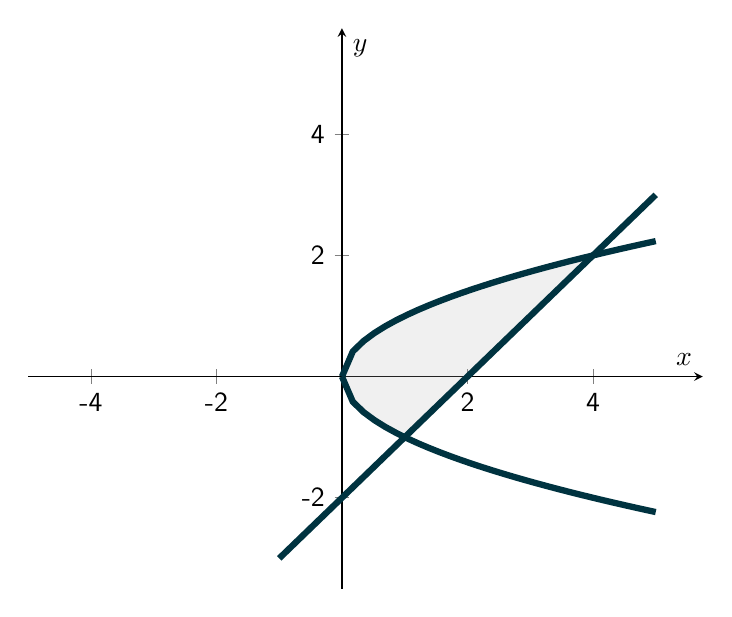
\begin{tikzpicture}[scale=1.25]
            \begin{axis}[
            axis lines = middle, very thick,
            xlabel = {$x$},
            ylabel = {$y$},
            xmin=-5, xmax=5.75,
            ymin=-3.5, ymax=5.75,
            xtick={-4,-2,0,2,4},
            xticklabels={-4,-2,0,2,4},
            ytick={-2,0,2,4},
            yticklabels={-2,0,2,4}        
            ]
            % Curves
            \addplot [name path = A,-,domain = 0:5, line width=0.8mm,DarkBlue,samples = 30] {sqrt(x)} ;
            \addplot [name path = B,-,domain = 0:5, line width=0.8mm,DarkBlue,samples = 30] {-sqrt(x)} ;
            \addplot [name path = C, line width=0.8mm, samples=4, smooth,domain=0:5, DarkBlue] coordinates {(-1,-3)(5,3)};
            % Fill area between paths
            \addplot [black!30, opacity=0.2] fill between [of = A and B, soft clip={domain=0:1}];
            \addplot [black!30, opacity=0.2] fill between [of = A and C, soft clip={domain=1:4}];
            \end{axis}
        \end{tikzpicture}    
    \end{center}   
        
    Thus
    \begin{align}
        \bar y &= \frac{M_x}M = \frac1M \int_{-1}^{2}\int_{y^2}^{y+2} 12y \, dx \, dy
    \end{align} 
    Thus
    \begin{align}
        a &= -1 \\
        b &= 2 \\
        c&= y^2 \\
        d&= y+2 \\
        f(x,y) &= \delta y = 12y
    \end{align}
    }
   \else

   \fi
    
\fi

\ifnum \Version=7
% SHORT SPHERICAL AND CYLINDRICAL EXERCISE
\part Point $P$ has rectangular (Cartesian) coordinates $(x,y,z) = (-6,0,8)$ in $\mathbb R^3$. In cylindrical coordinates, the point is $(r,\theta,z)$, and in spherical coordinates the point is $(\rho, \phi, \theta)$. Where $r=\framebox{\strut\hspace{1cm}}$, $\theta=\framebox{\strut\hspace{2cm}}$, $z=\framebox{\strut\hspace{1cm}}$, $\rho=\framebox{\strut\hspace{2cm}}$, and $\phi=\framebox{\strut\hspace{3cm}}$. 

    \ifnum \Solutions=1 {\color{DarkBlue} \textit{Solutions:} To convert to cylindrical we can use the equation $r^2 = x^2 + y^2$. 
    \begin{align}
        r^2 &= x^2 + y^2 = (-6)^2 + 0^2 = 36 \ \Rightarrow \ r = 6
    \end{align}
    To determine $\theta$ we can use $\tan\theta = y/x$. 
    \begin{align}
        \tan \theta &= \frac{y}{x} = \frac{0}{-6} = 0  \\
        \theta &= \arctan 0 
    \end{align} 
    The point in cylindrical is: 
    \begin{align}
        (r,\theta,z) &= (6,\pi,8) \\
        r &= 6 \\
        \theta &= \pi \\
        z &= 8
    \end{align}
    In spherical, we can start by obtaining $\rho$. 
    \begin{align}
        \rho^2 &= x^2+y^2+z^2\\
        \rho^2 &= (-6)^2 + 0^2 + 8^2 = 36+64 = 100 \\
        \rho &= 10
    \end{align}
    To obtain $\phi$ we can use the equation that relates $x$ to spherical. Using the expression for $x$, and the values that we already have for $x$, $\rho$ and $\theta$:
    \begin{align}
        x &= \rho \sin\phi \cos\theta \\
        -6 &= 10\sin\phi \cos(\pi) \\
        \sin\phi &= \frac{-6}{10 \cos(\pi)}  = \frac{6}{10}\\
        \phi &= \arcsin (6/10)
    \end{align}
    Our coordinates in spherical are
    \begin{align}
        \rho &= 10\\
        \phi &= \arcsin (6/10)\\
        \theta &= \pi
    \end{align}
    Note the following.
    \begin{itemize}
        \item We can, for this exercise, leave un-evaluated trig functions in the answer, because the question didn't specify that you should simplify your answer as much as possible. So it would be ok to leave your answer for $\theta$ as $\arctan 0$ or $\tan^{-1} 0$. 
        \item Our particular textbook uses the convention $(\rho, \phi, \theta)$, not $(\rho, \theta,\phi)$.
    \end{itemize}
    } 
    \else
      
    \fi
    
\fi





\ifnum \Version=8
% SHORT SPHERICAL AND CYLINDRICAL EXERCISE
\part Point $P$ has rectangular (Cartesian) coordinates $(x,y,z) = (4,4,7)$ in $\mathbb R^3$. In cylindrical coordinates, the point is $(r,\theta,z)$, and in spherical coordinates the point is $(\rho, \phi, \theta)$. Where $r=\framebox{\strut\hspace{1cm}}$, $\theta=\framebox{\strut\hspace{2cm}}$, $z=\framebox{\strut\hspace{1cm}}$, $\rho=\framebox{\strut\hspace{2cm}}$, and $\phi=\framebox{\strut\hspace{3cm}}$. 

    \ifnum \Solutions=1 {\color{DarkBlue} \textit{Solutions:} To convert to cylindrical we can use the equation $r^2 = x^2 + y^2$. 
    \begin{align}
        r^2 &= x^2 + y^2 = (4)^2 + 4^2 = 32 \ \Rightarrow \ r = \sqrt{32} = 4\sqrt2
    \end{align}
    It isn't necesssary to simplify to $4\sqrt2$. Then to determine $\theta$ we can use $\tan\theta = y/x$. 
    \begin{align}
        \tan \theta &= \frac{y}{x} = \frac{4}{4} = 1  \\
        \theta &= \arctan \pi/4
    \end{align} 
    The point in cylindrical is: 
    \begin{align}
        (r,\theta,z) &= (4\sqrt2,\pi/4,7) \\
        r &= 4\sqrt2 \\
        \theta &= \pi/4 \\
        z &= 7
    \end{align}
    In spherical, we can start by obtaining $\rho$. 
    \begin{align}
        \rho^2 &= x^2+y^2+z^2\\
        \rho^2 &= (4)^2 + 4^2 + 7^2 = 16+16+49 = 32+49 = 81 \\
        \rho &= 9
    \end{align}
    To obtain $\phi$ we can use the equation that relates $x$ to spherical. Using the expression for $x$, and the values that we already have for $x$, $\rho$ and $\theta$:
    \begin{align}
        x &= \rho \sin\phi \cos\theta \\
        4 &= 9\sin\phi \cos(\pi/4) \\
        \sin\phi &= \frac{4}{9 \cos(\pi/4)}  = \frac{4\sqrt2}{9}\\
        \phi &= \arcsin \left(\frac{4\sqrt2}{9}\right)
    \end{align}
    Note for $\phi$ we can also use:
    \begin{align}
        y &= \rho \sin\phi \sin\theta \\
        4 &= 9\sin\phi \sin(\pi/4) \\
        \sin\phi &= \frac{4}{9 \sin(\pi/4)}  = \frac{4\sqrt2}{9}\\
        \phi &= \arcsin \left(\frac{4\sqrt2}{9}\right)
    \end{align}    
    And we can also use:
    \begin{align}
        z &= \rho \cos\phi  \\
        7 &= 9\cos\phi  \\
        \sin\phi &= \frac{4}{9 \sin(\pi/4)}  = \frac{4\sqrt2}{9}\\
        \phi &= \arccos \left(\frac{7}{9}\right)
    \end{align}      
    Our coordinates in spherical are
    \begin{align}
        \rho &= 9\\
        \phi &= \arcsin \left(\frac{4\sqrt2}{9}\right), \ \textbf{or} \ \phi = \arccos(7/9)\\
        \theta &= \pi/4
    \end{align}
    Note the following.
    \begin{itemize}
        \item We can, for this exercise, leave un-evaluated trig functions in the answer, because the question didn't specify that you should simplify your answer as much as possible. So it would be ok to leave your answer for $\theta$ as $\arctan 1$ or $\tan^{-1} 1$. 
        \item Our particular textbook uses the convention $(\rho, \phi, \theta)$, not $(\rho, \theta,\phi)$.
    \end{itemize}
    } 
    \else
      
    \fi
    
\fi





% 15.6
% CENTROID Y-COORDINATE PARABOLA AND LINE
\ifnum \Version=9
    \part A thin plate with density $\delta=12$ is bounded in the $xy-$plane by $y=3-x^2$ and $y=1-x$. The plate has mass $M$. The $y-$coordinate of the centroid is $\bar y = M_x/M$, where $\displaystyle M_x = \int_A^B \int_C^D f(x,y) \, dy \, dx$,  and $A=\framebox{\strut\hspace{1cm}}$, $B=\framebox{\strut\hspace{1cm}}$, $C=\framebox{\strut\hspace{3cm}}$, $D=\framebox{\strut\hspace{3cm}}$, and $f(x,y) = \framebox{\strut\hspace{3cm}}$. 
    
    \ifnum \Solutions=1 
    {\color{DarkBlue}
    The region is bounded by 
    $$1-x \le y \le 3-x^2$$
    The given curves intersect when 
    \begin{align}
        1-x &= 3-x^2\\
        0 &= x^2-x-2 \\
        &= (x-2)(x+1)
    \end{align}
    The curves intersect at $x=-1,2$. Using $y=1-x$, the intersection points are $(-1,2)$ and $(2,-1)$. The region is shown below. 
    \begin{center}  
        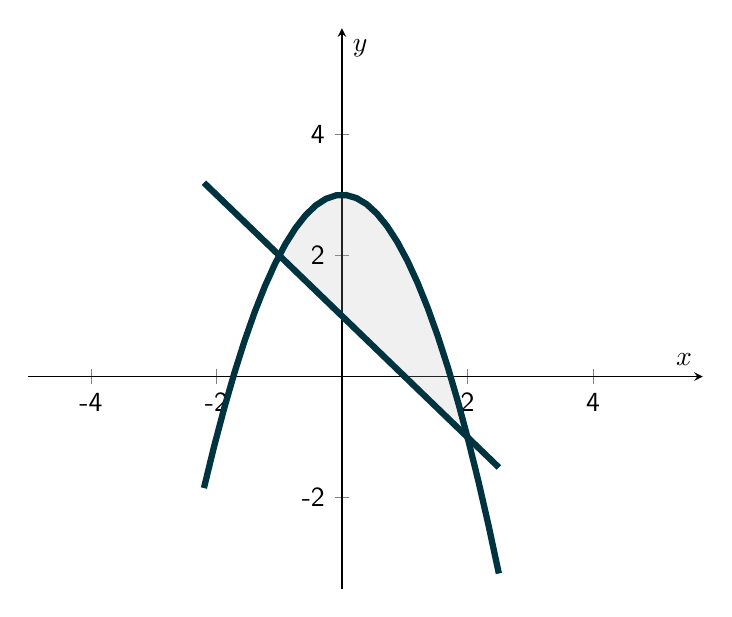
\begin{tikzpicture}[scale=1.25]
            \begin{axis}[
            axis lines = middle, very thick,
            xlabel = {$x$},
            ylabel = {$y$},
            xmin=-5, xmax=5.75,
            ymin=-3.5, ymax=5.75,
            xtick={-4,-2,0,2,4},
            xticklabels={-4,-2,0,2,4},
            ytick={-2,0,2,4},
            yticklabels={-2,0,2,4}        
            ]
            % Curves
            \addplot [name path = A,-,domain = -2.2:2.5, line width=0.8mm,DarkBlue,samples = 30] {3-x^2} ;
            \addplot [name path = C,-,domain = -2.2:2.5, line width=0.8mm,DarkBlue,samples = 4] {1-x} ;
            % Fill area between paths
            \addplot [black!30, opacity=0.2] fill between [of = A and C, soft clip={domain=-1:2}];
            \end{axis}
        \end{tikzpicture}    
    \end{center}   
        
    Thus
    \begin{align}
        \bar y &= \frac{M_x}M = \frac1M \int_{-1}^{2}\int_{1-x}^{3-x^2} 12y \, dy \, dx
    \end{align} 
    Thus
    \begin{align}
        A &= -1 \\
        B &= 2 \\
        C&= 1-x \\
        D&= 3-x^2 \\
        f(x,y) &= \delta y = 12y
    \end{align}
    }
   \else

   \fi
    
\fi
   
    % 13.3 and 13.4
% unit tangent vectors
% arc length
% curvature
% osculating circle
% unit normal

\ifnum \Version=1

\part The unit tangent vector for a curve $\mathbf r(t)$ is $\mathbf T(t) = \langle 0, \cos t, \sin t \rangle$. The unit normal vector is $\mathbf  N = \langle f(t), g(t), g(t) \rangle$, where $f(t) = \framebox{\strut\hspace{2cm}}$, $g(t) = \framebox{\strut\hspace{2cm}}$, $h(t) =\framebox{\strut\hspace{2cm}}$. 

\ifnum \Solutions=1 {\color{DarkBlue} \textit{Answer:} \textit{Solutions:} The normal vector is

\begin{align}
    \mathbf N &= \frac{d\mathbf T/dt}{|d\mathbf T/dt|} 
\end{align}
And
\begin{align}
    \mathbf T'(t) &= \langle 0,-\sin t, \cos t \rangle \\
    |\mathbf T'(t) | &= \sqrt{ 0 +(-\sin t)^2 + (\cos t)^2} =1\\
    \mathbf N &= \frac{d\mathbf T/dt}{|d\mathbf T/dt|} = \langle 0, - \sin(t),  \cos(t) \rangle
\end{align}
} 
\else
\fi        
\fi

\ifnum \Version=2

\part The velocity vector of an object moving on the curve $\mathbf r(t)$ is $\mathbf v(t) = \langle 4\cos (2t), 4\sin (2t) , 3 \rangle$ for $t>0$. The speed of the object for $t>0$ is $s(t) = |\mathbf v | = \framebox{\strut\hspace{1cm}}$. The unit tangent vector for $t>0$ is $\mathbf T = \langle f(t), g(t) , h(t) \rangle$, where $f(t) = \framebox{\strut\hspace{1.5cm}}$, $g(t) = \framebox{\strut\hspace{1.5cm}}$, $h = \framebox{\strut\hspace{1cm}}$. The curvature is $\kappa = \framebox{\strut\hspace{1cm}}$. 

\ifnum \Solutions=1 {\color{DarkBlue} \textit{Answer:} \textit{Solutions:} The speed is the magnitude of the given velocity vector and is
\begin{align}
    s &= |\mathbf v | =  \sqrt{(4\cos2t)^2 + (4\sin2t)^2 + 3^2 } = \sqrt{4^2 (\cos ^2 2 t + \sin^2 2t) + 3^2} = \sqrt{16 + 9} = 5
\end{align}
The unit tangent vector is 
\begin{align}
    \mathbf T &= \frac{\mathbf v}{|\mathbf v|} = \langle \frac{4}{5}\cos(2 t) , \frac 45 \sin (2t), \frac35 \rangle
\end{align}
For curvature we also need
\begin{align}
    \frac{d\mathbf T}{dt } &= \langle -\frac85 \sin 2t, \frac85 \cos 2t,0 \rangle \\
    \left | \frac{d\mathbf T}{dt } \right| &= \sqrt{ \left(-\frac85\sin 2t\right)^2 +   \left(\frac85 \cos 2 t\right)^2 } = \frac85
\end{align}
The curvature is
\begin{align}
    \kappa = \frac{1}{|\mathbf v |}\left| \frac{d\mathbf T}{dt}\right| = \frac{1}{5} \cdot \frac{8}{5} = \frac{8}{25}
\end{align}
} 
\else
\fi        
\fi


\ifnum \Version=3

\part A plane curve $\mathbf r(t)$ has curvature $\kappa = \frac{1}{8}$ at $\mathbf r(t_0) = \langle 15, 2 \rangle$, and the unit normal vector at $t=t_0$ is $\mathbf  N = \mathbf j = \langle 0, 1 \rangle$. The equation of the osculating circle at $t=t_0$ is \framebox{\strut\hspace{3.5cm}}.

\ifnum \Solutions=1 {\color{DarkBlue} \textit{Answer:} \textit{Solutions:} Recall that The circle of curvature, or osculating circle, at a point $P$ on a plane curve where $\kappa \ne 0$ is the circle in the plane of the curve that

\begin{enumerate}
    \item is tangent to the curve at P (has the same tangent line the curve has)
    \item has the same curvature the curve has at P
    \item lies toward the concave or inner side of the curve
\end{enumerate}
The \textbf{radius of curvature} of the curve at P is the radius of the circle of curvature, which is $\frac{1}{\kappa}$. So to obtain the radius, we calculate $\kappa$ and take the reciprocal. The \textbf{center} of the osculating circle of the curve at P lies on the inner side of the curve, and the unit normal points in the direction of the inner side of the planar curve. 

So for this problem we have a circle with radius $1/\kappa = 8$, and whose centre is 8 units away from the point $(15,2)$ in the direction of $\mathbf N$. The circle has equation
$$(x-15)^2 + (y-10)^2 = 8^2$$
} 
\else
  
\fi        
\fi




\ifnum \Version=4

\part The velocity vector for an object moving on the curve $\mathbf r(t)$ is $\mathbf v(t) = \langle t\cos t, t\sin t \rangle$. The speed of the object for $t>0$ is $s(t) = \framebox{\strut\hspace{1cm}}$. The unit tangent vector for $t>0$ is $\mathbf T = \langle f(t), g(t) \rangle$, where $f(t) = \framebox{\strut\hspace{2cm}}$, $g(t) = \framebox{\strut\hspace{2cm}}$. 

\ifnum \Solutions=1 {\color{DarkBlue} \textit{Answer:} \textit{Solutions:} The speed is the magnitude of the velocity vector and is
\begin{align}
    s &= |\mathbf v | = \sqrt{(t\cos t)^2 + (t\sin t)^2 } = \sqrt{t^2 (\cos ^2 t + \sin^2 t)} = |t|
\end{align}
But we are told that $t>0$ so we can use $|t| = t$. The unit tangent vector is 
\begin{align}
    \mathbf T &= \frac{\mathbf v}{|\mathbf v|} = \langle \cos t, \sin t \rangle
\end{align}
} 
\else
\fi        
\fi

\ifnum \Version=5

\part A plane curve $\mathbf r(t)$ has curvature $\kappa = \frac{1}{4}$ at the point $\mathbf r(t_0) = 3\mathbf i + 5\mathbf j$, and the unit normal vector at $t_0$ is $\mathbf  N = \mathbf i = \langle1,0\rangle$. The equation of the osculating circle at $t=t_0$ is \framebox{\strut\hspace{3.5cm}}.

\ifnum \Solutions=1 {\color{DarkBlue} \textit{Answer:} \textit{Solutions:} Recall that The circle of curvature, or osculating circle, at a point $P$ on a plane curve where $\kappa \ne 0$ is the circle in the plane of the curve that

\begin{enumerate}
    \item is tangent to the curve at P (has the same tangent line the curve has)
    \item has the same curvature the curve has at P
    \item lies toward the concave or inner side of the curve
\end{enumerate}
The \textbf{radius of curvature} of the curve at P is the radius of the circle of curvature, which is $\frac{1}{\kappa}$. So to obtain the radius, we calculate $\kappa$ and take the reciprocal. The \textbf{center} of the osculating circle of the curve at P lies on the inner side of the curve, and the unit normal points in the direction of the inner side of the planar curve. 

So for this problem we have a circle with radius $1/\kappa = 4$, and whose centre is 4 units away from the point $(3,5)$ in the direction of $\mathbf N$. The circle has equation
$$(x-7)^2 + (y-5)^2 = 4^2$$
} 
\else
  
\fi        
\fi


\ifnum \Version=6

\part The velocity vector for an object moving on the curve $\mathbf r(t)$ is $\mathbf v(t) = \langle 4t\cos t, 4t\sin t \rangle$ for $t>0$. The speed of the object for $t>0$ is $s(t)  = |\mathbf v | = \framebox{\strut\hspace{1cm}}$. The unit tangent vector for $t>0$ is $\mathbf T = \langle f(t), g(t) \rangle$, where $f(t) = \framebox{\strut\hspace{1.5cm}}$, $g(t) = \framebox{\strut\hspace{1.5cm}}$. The curvature is $\kappa = \framebox{\strut\hspace{1cm}}$. 

\ifnum \Solutions=1 {\color{DarkBlue} \textit{Answer:} \textit{Solutions:} The speed is the magnitude of the given velocity vector and is
\begin{align}
    s &= |\mathbf v | =  \sqrt{(4t\cos t)^2 + (4t\sin t)^2 } = \sqrt{4^2t^2 (\cos ^2 t + \sin^2 t)} = 4|t|
\end{align}
But we are told that $t>0$ so we can assume $|t| = t$. The unit tangent vector is 
\begin{align}
    \mathbf T &= \frac{\mathbf v}{|\mathbf v|} = \langle \cos t, \sin t \rangle
\end{align}
We need
\begin{align}
    \frac{d\mathbf T}{dt } &= \langle -\sin t, \cos t \rangle \\
    \left | \frac{d\mathbf T}{dt } \right| &= \sqrt{ (-\sin t)^2 +   \cos^2 t } = 1
\end{align}
The curvature is
\begin{align}
    \kappa = \frac{1}{|\mathbf v |}\left| \frac{d\mathbf T}{dt}\right| = \frac{1}{4t} 
\end{align}
} 
\else
\fi        
\fi



\ifnum \Version=7

\part The velocity vector of an object moving on the curve $\mathbf r(t)$ is $\mathbf v(t) = \langle 3\cos (2t), 3\sin (2t) \rangle$ for $t>0$. The speed of the object for $t>0$ is $s(t) = |\mathbf v | = \framebox{\strut\hspace{1.5cm}}$. The unit tangent vector for $t>0$ is $\mathbf T = \langle f(t), g(t)  \rangle$, where $f(t) = \framebox{\strut\hspace{2cm}}$, and $g(t) = \framebox{\strut\hspace{2cm}}$.  The curvature for $t>0$ is \framebox{\strut\hspace{1.5cm}}. 

\ifnum \Solutions=1 {\color{DarkBlue} \textit{Answer:} \textit{Solutions:} The speed is the magnitude of the given velocity vector and is
\begin{align}
    s &= |\mathbf v | =  \sqrt{(3\cos t)^2 + (3\sin t)^2  } = \sqrt{3^2 (\cos ^2 t + \sin^2 t) + 3^2} = \sqrt{ 9} = 3
\end{align}
The unit tangent vector is 
\begin{align}
    \mathbf T &= \frac{\mathbf v}{|\mathbf v|} 
    = \langle \frac{3}{3}\cos(2 t) , \frac 33 \sin (2t) \rangle 
    = \langle \cos(2 t) ,  \sin (2t) \rangle
\end{align}
For curvature we also need
\begin{align}
    \frac{d\mathbf T}{dt } &= \langle -2 \sin 2t, 2 \cos 2t\rangle \\
    \left | \frac{d\mathbf T}{dt } \right| &= \sqrt{ \left(-2\sin 2t\right)^2 +   \left(2 \cos 2 t\right)^2 } = 2
\end{align}
The curvature is
\begin{align}
    \kappa = \frac{1}{|\mathbf v |}\left| \frac{d\mathbf T}{dt}\right| = \frac{1}{3} \cdot 2 = \frac{2}{3}
\end{align}
} 
\else
\fi        
\fi


\ifnum \Version=8

\part A plane curve $\mathbf r(t)$ has curvature $\kappa = \frac{1}{4}$ at $\mathbf r(t_0) = \langle 5, 3 \rangle$, and the unit normal vector at $t=t_0$ is $\mathbf  N = \mathbf j = \langle 0, 1 \rangle$. The equation of the osculating circle at $t=t_0$ is \framebox{\strut\hspace{3.5cm}}.

\ifnum \Solutions=1 {\color{DarkBlue} \textit{Answer:} \textit{Solutions:} Recall that The circle of curvature, or osculating circle, at a point $P$ on a plane curve where $\kappa \ne 0$ is the circle in the plane of the curve that

\begin{enumerate}
    \item is tangent to the curve at P (has the same tangent line the curve has)
    \item has the same curvature the curve has at P
    \item lies toward the concave or inner side of the curve
\end{enumerate}
The \textbf{radius of curvature} of the curve at P is the radius of the circle of curvature, which is $\frac{1}{\kappa}$. So to obtain the radius, we calculate $\kappa$ and take the reciprocal. The \textbf{center} of the osculating circle of the curve at P lies on the inner side of the curve, and the unit normal points in the direction of the inner side of the planar curve. 

So for this problem we have a circle with radius $1/\kappa = 4$, and whose centre is 4 units away from the point $(5,3)$ in the direction of $\mathbf N$. The circle has equation
$$(x-5)^2 + (y-7)^2 = 4^2$$
} 
\else
  
\fi        
\fi






\ifnum \Version=9

\part The velocity vector of an object moving on the curve $\mathbf r(t)$ is $\mathbf v(t) = \langle t, 3 \rangle$ for $t>0$. The speed of the object at $t=2$ is $s(2) = |\mathbf v(2) | = \framebox{\strut\hspace{1.75cm}}$. The unit tangent vector at $t=2$ is $\mathbf T(2) = \langle c_1 ,c_2  \rangle$, where $c_1 = \framebox{\strut\hspace{1.75cm}}$, $c_2 = \framebox{\strut\hspace{1.75cm}}$. The curvature is $\framebox{\strut\hspace{1.75cm}}$. 

\ifnum \Solutions=1 {\color{DarkBlue} \textit{Answer:} \textit{Solutions:} The speed is the magnitude of the given velocity vector and is
\begin{align}
    s &= |\mathbf v | =  \sqrt{( t)^2 + (3)^2  } = \sqrt{t^2+9}\\
    s(2) &= \sqrt{2^2+9} = \sqrt{13}
\end{align}
We also need the unit tangent vector at $t=2$. 
\begin{align}
    \mathbf T (t) &= \frac{\mathbf v}{|\mathbf v|} = \frac{t\mathbf i + 3\mathbf j}{\sqrt{t^2+9}} \\
    \mathbf T (2) &= \frac{2\mathbf i + 3\mathbf j}{\sqrt{2^2+9}}  
    = \langle \frac{2}{\sqrt{13}} , \frac {3}{\sqrt{13}}  \rangle \\
    c_1 &= \frac{2}{\sqrt{13}}\\
    c_2 &= \frac{3}{\sqrt{13}}
\end{align}
The curvature is zero because the motion is along a straight line. 
\begin{align}
    \kappa = 0
\end{align}
} 
\else
\fi        
\fi

\ifnum \Version=10

\part A plane curve $\mathbf r(t)$ has curvature $\kappa = \frac{1}{10}$ at $\mathbf r(t_0) = \langle 5, 0 \rangle$, and the unit normal vector at $t=t_0$ is $\mathbf  N = \mathbf j = \langle 0, 1 \rangle$. The equation of the osculating circle at $t=t_0$ is \framebox{\strut\hspace{3.5cm}}.

\ifnum \Solutions=1 {\color{DarkBlue} \textit{Answer:} \textit{Solutions:} Recall that The circle of curvature, or osculating circle, at a point $P$ on a plane curve where $\kappa \ne 0$ is the circle in the plane of the curve that

\begin{enumerate}
    \item is tangent to the curve at P (has the same tangent line the curve has)
    \item has the same curvature the curve has at P
    \item lies toward the concave or inner side of the curve
\end{enumerate}
The \textbf{radius of curvature} of the curve at P is the radius of the circle of curvature, which is $\frac{1}{\kappa}$. So to obtain the radius, we calculate $\kappa$ and take the reciprocal. The \textbf{center} of the osculating circle of the curve at P lies on the inner side of the curve, and the unit normal points in the direction of the inner side of the planar curve. 

So for this problem we have a circle with radius $1/\kappa = 10$, and whose centre is 10 units away from the point $(5,0)$ in the direction of $\mathbf N$. The circle has equation
$$(x-5)^2 + (y-10)^2 = 10^2$$
} 
\else
  
\fi        
\fi
   
\end{parts}

\newpage \question[0.25] \ID
% CHANGE OF VARIABLE (15.8)
% OR APPLICATION (15.6)
% OR TRIPLE CARTESIAN (15.5) 

\ifnum \Version=1
% CENTROID
% BASED ON THOMAS EXERCISES, 15.6 #1
% SUFFICIENT FOR A PRACTICE EXAM
\question[6] A thin plate of density $\delta(x,y) = 12x$ is bounded by the lines $x = 0, y = x$, and the parabola $y = x^2-6$ in the first quadrant. 
\begin{parts} 
    \part Determine the mass of the plate, $M$. Please show your work. 
    \ifnum \Solutions=1 
    {\color{DarkBlue} \textit{Solutions:}
    Curves intersect when $$x = x^2-6 \quad \Rightarrow \quad 0 = x^2 - x - 6 = (x-3)(x+2)$$
    Or $x=3, -2$. We can ignore $x=-2$ because the region is the first quadrant. Curves intersect at the point $(3,3)$, and 
    \begin{align}
        0 \le y \le 3, \quad y \le x \le \sqrt{y+6}
    \end{align}
    The mass is
    \begin{align}
        M &= \int_0^3 \int_y^{\sqrt{y+6}} \delta \, dx \, dy \\
        &= \int_0^3 \int_y^{\sqrt{y+6}} 12x \, dx \, dy \\
        &= \int_0^3  \left. 6x^2 \right|_{x=y}^{x=\sqrt{y+6}} \, dy \\
        &= \int_0^3 6(y + 6 - y^2) \, dy \\
        &= \int_0^3 6y + 36 - 6y^2 \, dy \\
        &= \left. (3y^2 + 36y - 2y^3 ) \right|_0^3 \, dy \\
        &= 27 + 108 - 54 \\
        &= 81
    \end{align}
    }
    \else 
    \vspace{16cm}
    \fi
    \part Use your results from the previous part to set up an integral that can be used to determine the $x-$coordinate of the center of mass of the plate. You do not need to evaluate your integral. 
    \ifnum \Solutions=1 {\color{DarkBlue} \textit{Solutions:} the $x-$coordinate of the center of mass, $\bar x$, is
    \begin{align}
    \bar x &= \frac{M_y}{M} = \frac{1}{81} \int_0^3 \int_y^{\sqrt{y+6}} 12x^2 \, dx \, dy 
    \end{align}
    } 
    \else
      
    \fi
    \end{parts} 
\fi
    





\ifnum \Version=2
% LONGISH CHANGE OF VARIABLE
% VERBATUM FROM SPRING 2022 QUIZ
% hand written solution only
% SUFFICIENT FOR A PRACTICE EXAM
\question[6] Consider the double integral

$$I=\iint_R \frac{x+2y}{2y-x} dA$$

where $R$ is the parallelogram with vertices $(-3,1), (-1,0), (-1,2), (1,1)$. Our goal is to determine the area of the parallelogram using the transform below. 
$$u=x+2y, \qquad v = -x +2y$$ 
Please show your work for the following. 
\begin{parts} 
    \part Use the given transform to calculate the Jacobian of the transform, $J = \partial x(u,v)/\partial y(u,v)$. 
    \ifnum \Solutions=1 
    \else 
    \vspace{8 cm}
    \fi
    \part Use your results from Part (a) and the given transform to transform the double integral. You do not need to evaluate your integral. 
\end{parts} 

\ifnum \Solutions=1 {\color{DarkBlue} \textit{Solutions:} the integral after the transform is $$\displaystyle \frac14 \int_1^5\int_{-1}^3 \frac uv \, du \, dv$$
A screen capture of a hand-written solution from a previous offer of MATH 2551 is below. 
    \begin{figure}[h]
    \centering
    \includegraphics[width=16cm]{202302/Exam3/Images/ImgE3.OR.06.png}
    \end{figure}  
    
    } 
   \else
      
   \fi
    
\fi

\ifnum \Version=3
% CENTROID
% BASED ON THOMAS EXERCISES, 15.6 #1
% SUFFICIENT FOR A PRACTICE EXAM
\question[6] A thin plate with density $\delta(x,y) = 24y$ is bounded by the lines $x = 0, x=2y$, and the parabola $x=y^2$ in the first quadrant. 
\begin{parts} 
    \part Determine the mass of the plate, $M$. Please show your work. 
    
    \ifnum \Solutions=1 
    {\color{DarkBlue} \textit{Solutions:}
    Curves intersect when $$2y = y^2 \quad \Rightarrow \quad 0 = y^2-2y = y(y-2)$$
    Or $y=0,2$. Curves intersect at the points $(0,0)$, $(4,2)$. 
    The mass is
    \begin{align}
        M = \int_0^4 \int_{x/2}^{\sqrt{x}} \delta \, dy \, dx 
        &= \int_0^4 \int_{x/2}^{\sqrt{x}} 24y \, dy \, dx \\
        &= \int_0^4  \left. 12y^2 \right|_{y=x/2}^{y=\sqrt{x}} \, dx \\
        &= 12 \int_0^4 (x-\frac{x^2}{4}) \, dx \\
        &= 12 \left. (\frac{x^2}{2} - \frac{x^3}{12} ) \right|_0^4 \, dy \\
        &= 12 (\frac{16}{2} - \frac{64}{12}) \\
        &= 96 - 64\\
        &= 32
    \end{align}
    \textbf{An Alternate Solution}\\
    Another way to approach this problem is to use the integration order $dx\,dy$. In this case the double integral becomes
    \begin{align}
        M = \int_0^2 \int_{y^2}^{2y} \delta \, dx \, dy
        &= \int_0^2 \int_{y^2}^{2y} 24y \, dx \, dy \\
        &= 24\int_0^2  \left. yx \right|_{x=y^2}^{x=2y} \, dy \\
        &= 24 \int_0^2 (2y^2 - y^3) \, dy \\
        &= 24 \left. (\frac{2y^3}{3} - \frac{y^4}{4} ) \right|_0^2 \, dy \\
        &= 24 (\frac{16}{3} - \frac{16}{4}) \\
        &= \frac{24\cdot16}{3} - 24\cdot 4 \\
        &= 8\cdot16 - 96 \\
        &= 128 - 96 \\
        &= 32
    \end{align}    
    }
    \else 
    \vspace{14cm}
    \fi
    \part Use your results from the previous part to set up an integral that can be used to determine the $x-$coordinate of the center of mass of the plate. You do not need to evaluate your integral. 
    \ifnum \Solutions=1 {\color{DarkBlue} \textit{Solutions:} the $x-$coordinate of the center of mass, $\bar x$, is
    \begin{align}
    \bar x &= \frac{M_y}{M} = \frac{1}{32} \int_0^4 \int_{x/2}^{\sqrt{x}} 24xy \, dy \, dx
    \end{align}
    \textbf{An Alternate Solution}\\    
    It is also ok to use the integration order $dx\,dy$. In this case the double integral becomes
    \begin{align}
    \bar x &= \frac{M_y}{M} = \frac{1}{32} \int_0^2 \int_{y^2}^{2y} 24xy \, dx \, dy 
    \end{align}
    } 
    \else
      
    \fi
    \end{parts} 
\fi

\ifnum \Version=4
% VERSION B
% LONG CHANGE OF VARIABLE
% BASED ON AN EXAMPLE FROM THOMAS
% SECTION 15.8 FROM THOMAS
\question[6] Consider the double integral

$$I= 9 \iint_R (y-2x)^2 \sqrt{x+y} \, dA$$

where $R$ is the region in the first quadrant bounded by the lines $x=0$, $y=0$, and $y=1-x$. Our goal is to determine the area of $R$ using the transform below. 
$$u=x+y, \qquad v = y-2x$$ 
Please show your work for the following. 
\begin{parts} 
    \part Use the given transform to calculate the Jacobian of the transform, $J = \partial x(u,v)/\partial y(u,v)$. 
    \ifnum \Solutions=1 {\color{DarkBlue} \textit{Solutions:} Solving for $x$ and $y$ using an augmented matrix,
    \begin{align}
        \begin{pmatrix} 1 & 1 & u \\-2 & 1 & v\end{pmatrix} 
        \sim \begin{pmatrix} 1 & 1 & u \\0 & 3 & 2u+v\end{pmatrix} 
        \sim \begin{pmatrix} 1 & 0 & u/3 - v/3 \\0 & 1 & 2u/3+v/3 \end{pmatrix} 
    \end{align}
    Thus
    \begin{align}
        x &= \frac13(u-v), \ y = \frac13(2u+v) \\
        J(u,v) & = \begin{vmatrix} \DXDU & \DXDV \\[8pt] \DYDU & \DYDV \end{vmatrix} = \begin{vmatrix} 1/3 & -1/3 \\ 2/3 & 1/3 \end{vmatrix} = 1/9 + 2/9 = 1/3
    \end{align}
    }
    \else 
    \vspace{8 cm}
    \fi
    \part Use the given transform and your results from Part (a) to convert the double integral into a double integral over a region in the $uv-$plane. You do not need to evaluate your integral. 
    \ifnum \Solutions=1 {\color{DarkBlue} \textit{Solutions:} Converting each of the boundaries in the $xy-$plane into the $uv-$plane we obtain
        \begin{align}
            x+y &= 1 \quad \Rightarrow \quad \frac13(u-v) + \frac13(2u+v) = 1 &&\Rightarrow \quad u = 1\\
            x&=0 \quad \Rightarrow \quad \frac13(u-v) = 0 &&\Rightarrow \quad v = u\\
            y&= 0 \quad \Rightarrow \quad \frac13(2u+v) = 0 &&\Rightarrow \quad v = -2u
        \end{align}
        The region is described by either of the following relations:
        \begin{align}
            S_1: & \quad 0 \le u \le 1, \quad -2u \le v \le u \\
            S_2: & \quad -2 \le v \le 0, \quad -v/2 \le u \le 1, \ \text{and } 0 \le v \le 1, \quad v \le u \le 1
        \end{align}
        The first set of inequalities requires only a single double integral, but it is ok to set up two double integrals. If using $S_1$, we use $dv\,du$ and obtain
        \begin{align}
            I= 9 \iint_R (y-2x)^2 \sqrt{x+y} \, dA = 9 \int_0^1 \int_{-2u}^u v^2u^{1/2} \frac13 \,dv\,du
        \end{align}
        If using $S_2$, we use $du\,dv$ and obtain
        \begin{align}
            I= 9 \iint_R (y-2x)^2 \sqrt{x+y} \, dA 
            = 9 \int_{-2}^0 \int_{-v/2}^1 v^2u^{1/2} \frac13 \,du\,dv
            + 9 \int_{0}^1 \int_{v}^1 v^2u^{1/2} \frac13 \,du\,dv
        \end{align}        
        } 
       \else
          
       \fi
    \end{parts} 

    \fi



\ifnum \Version=5
    % USE FOR VERSION B
    % LONG CYLINDRICAL WITH APPLICATION TO MASS WITH VARYING DENSITY
    % FROM 15.8
    \question[6] An object $D$ lying in the first octant is bounded below by the $xy-$plane, above by the plane $z=3+4y$, and by the cylinder $x^2+y^2 = 4$. The density of the object at any point in $D$ is equal to the distance from the point to the $z$-axis.  Please show your work for the following.
    
    \begin{parts} 
    \part Use cylindrical coordinates to calculate the total of mass of the object, $M$. Please show your work. 
    
    \ifnum \Solutions=1 {\color{DarkBlue} The object is only in the first octant so $$0 \le \theta \le \pi/2$$ Using $\delta = \sqrt{x^2+y^2} = r$, the $z-$coordinate of the center of mass is computed using 
    \begin{align}
        M &= \iiint_D  \delta \, dV \\
        &= \int_0^{\pi/2} \int_0^2 \int_0^{3+4r\sin\theta}  \delta(r,\theta) \, r\, dz\,dr\,d\theta\\
        &= \int_0^{\pi/2} \int_0^2 \int_0^{3+4r\sin\theta}   r^2 \, dz\,dr\,d\theta\\
        &= \int_0^{\pi/2} \int_0^2    r^2 \, (3+4r\sin\theta) \,dr\,d\theta \\
        &= \int_0^{\pi/2} \int_0^2     \, (3r^2+4r^3\sin\theta) \,dr\,d\theta \\
        &= \int_0^{\pi/2}  \left. \, (r^3+r^4\sin\theta) \right|_{r=0}^{r=2} d\theta \\
        &= \int_0^{\pi/2}  (8 + 16\sin\theta) d\theta \\
        &=  \left. (8\theta - 16\cos\theta) \right|_0^{\pi/2} \\
        &=  (4\pi - 0) - (0 - 16) \\
        &= 4\pi + 16
    \end{align}
    
    } 
    \else
        \vspace{14cm}
    \fi
    
    \part Use your results from the previous part to set up a triple integral in cylindrical coordinates that can be used to determine the $z-$coordinate of the center of mass of the object. You do not need to evaluate your integral. 

    \ifnum \Solutions=1 {\color{DarkBlue} \textit{Solutions:} the $z-$coordinate of the center of mass, $\bar x$, is
    \begin{align}
    \bar z &= \frac{M_{xy}}{M} = \frac{1}{16\pi+16} \int_0^{\pi/2} \int_0^2 \int_0^{3+4r\sin\theta}  z \, \delta(r,\theta) \, r\, dz\,dr\,d\theta
    \end{align}
    } 
    \else
      
    \fi
    \end{parts} 
\fi


% TRANSFORM: SOLVE FOR X & Y, BOUNDARIES, EVALUATE, TRIANGLES
% VERSION A
\ifnum \Version=6
    \question[6] Consider the transform $u=x+y$ and $v=4x+5y$, and the integral $\displaystyle I = \iint_{R}  \,dxdy$. Region $R$ is the triangle in the $xy$-plane bounded by $x+y=0$, $4x+5y=0$, $6x+7y=4$. The transform maps $R$ to region $G$ in the $uv-$plane.  Please show your work for the following.

    \begin{enumerate}
        \item[a)] Solve the system, $u=x+y$ and $v=4x+5y$, for $x$ and $y$ in terms of $u$ and $v$.
            \ifnum \Solutions=1 {\color{DarkBlue} \\[12pt] 
            \textbf{Solutions:}
            We can use the expressions for $u$ and $v$ as an augmented matrix and row reduce. 
            \begin{align}
                \begin{pmatrix} 1 & 1 & u \\ 4 & 5 & v\end{pmatrix} 
                \sim \begin{pmatrix} 1 & 1 & u \\0 & 1 & v - 4u \end{pmatrix} 
                \sim \begin{pmatrix} 1 & 0 & 5u - v \\ 0 & 1 & v - 4u \end{pmatrix} 
            \end{align}
            Thus $x = 5u - v$, and $y = v - 4u$. 
            } 
            \else 
            \vspace{5cm}
            \fi
        \item[b)] Transform the boundaries of $R$ to the $uv-$plane. In other words, determine the boundaries of $G$ in terms of $u$ and $v$. 
            \ifnum \Solutions=1 {\color{DarkBlue} \\[12pt] 
            \textbf{Solutions:} the three lines are transformed below. 
            \begin{itemize}
                \item The line $x+y=0$ becomes $u=0$. 
                \item The line $4x+5y=0$ becomes $v=0$. 
                \item The line $6x+7y=4$ is: 
                \begin{align}
                    6x+7y &=4 \\
                    6\cdot(5u-v) + 7\cdot(v-4u) &= 4\\
                    30u -28u -6v+7v &=4 \\
                    v &= 4 -2u
                \end{align}
            \end{itemize}
            } 
        \else 
        \vspace{5cm}
        \fi        
            
        \item[c)] Use the given transformation and your results from parts (a) and (b) to set up a double integral that in the $uv-$plane that is equal to $I$. Do not evaluate the integral. You also do not need to calculate the Jacobian and may use that the Jacobian of the transform is $J(u,v) = 1$.
            \ifnum \Solutions=1 {\color{DarkBlue} \\[12pt] 
            \textbf{Solutions:}
            \begin{align}
                \iint_{R} \,dx\,dy
                &= \iint_{G}  \left| J(u,v) \right| \,dv\,du 
                = \int_0^2\int_{0}^{4-2u}  \left| 1 \right| \,dv\,du 
                = \int_0^2\int_{0}^{4-2u} \,dv\,du
            \end{align}
            Note the following.
            \begin{itemize}
                \item We did not need to compute the Jacobian but it is computed as follows. 
                $$J 
                = \begin{vmatrix} x_u & x_v \\ y_u & y_v \end{vmatrix} 
                = \begin{vmatrix} 5 & -1 \\ -4 & 1\end{vmatrix} 
                = 5 - 4
                = 1$$
                \item             We did not need to evaluate the integral but if we did:
            \begin{align}
                I = \int_0^2\int_{0}^{4-2u}  \left| 1 \right| \,dv\,du
                = 1 \int_0^2 (4-2u) \,du
                =  \left. 4u - u^2 \right|_0^2 
                = 4
            \end{align}
            \item It is also ok to use the other integration order: $I = \int_0^4\int_0^{2-v/2} \, du \, dv$.
            \end{itemize}
            } 
            \else 
            \fi        
    \end{enumerate}
 
\fi 



% TRANSFORM: SOLVE FOR X & Y, BOUNDARIES, EVALUATE, PARALLELOGRAM
% VERSION A
\ifnum \Version=7
    \question[6] Consider the integral $\displaystyle I = 2\iint_{R} x-4y \,dx\,dy$, where $R$ is the parallelogram in the $xy$-plane bounded by $x-4y=2$, $x-4y=1$, $3y-x=3$, $3y-x=6$. Suppose the transform $u=x-4y$ and $v=3y-x$, maps region $R$ to region $G$ in the $uv-$plane.  Please show your work for the following.

    \begin{enumerate}
        \item[a)] Solve the system, $u=x-4y$ and $v=3y-x$, for $x$ and $y$ in terms of $u$ and $v$.
            \ifnum \Solutions=1 {\color{DarkBlue} \\[12pt] 
            \textbf{Solutions:}
            We can use the expressions for $u$ and $v$ as an augmented matrix and row reduce. 
            \begin{align}
                \begin{pmatrix} 1 & -4 & u \\ -1 & 3 & v\end{pmatrix} 
                \sim \begin{pmatrix} 1 & -4 & u \\0 & -1 & v + u\end{pmatrix} 
                \sim \begin{pmatrix} 1 & 0 & -3u-4v\\0 & 1 & -u-v\end{pmatrix} 
            \end{align}
            Thus
            \begin{align}
                x &=  -3u-4v\\
                y &= -u-v
            \end{align}

            } 
            \else 
            \vspace{5cm}
            \fi
        \item[b)] Transform the boundaries of $R$ to the $uv-$plane. In other words, determine the boundaries of $G$ in terms of $u$ and $v$. 
            \ifnum \Solutions=1 {\color{DarkBlue} \\[12pt] 
            \textbf{Solutions:} the four lines are transformed below. 
            \begin{itemize}
                \item The line $x-4y=2$ becomes $u=2$. 
                \item The line $x-4y=1$ becomes $u=1$. 
                \item The line $3y-x=3$ becomes $v=3$. 
                \item The line $3y-x=6$ becomes $v=6$. 
            \end{itemize}
            } 
        \else 
        \vspace{5cm}
        \fi        
            
        \item[c)] Use the given transformation and your results from parts (a) and (b) to set up a double integral that in the $uv-$plane that is equal to $I$. Do not evaluate the integral. You also do not need to calculate the Jacobian and may use that the Jacobian of the transform is  $J(u,v) = -1$. 
            \ifnum \Solutions=1 {\color{DarkBlue} \\[12pt] 
            \textbf{Solutions:}
            \begin{align}
                \iint_{R} 2x-8y \,dx\,dy
                = \iint_{G} 2u \left| J(u,v) \right| \,du\,dv
                = \int_3^6\int_{1}^2 2u \left| -1 \right| \,du\,dv
                = \int_3^6\int_{1}^2 2u \,du\,dv
            \end{align}
            Note the following.
            \begin{itemize}
                \item We did not need to evaluate the integral, but if we did: 
                \begin{align}
                \iint_{R} 2x-8y \,dx\,dy
                &= \iint_{G} 2u \left| J(u,v) \right| \,du\,dv\\
                &= \int_3^6\int_{1}^2 2u \left| -1 \right| \,du\,dv\\
                &= \int_3^6\left. u^2 \right|_{1}^2 \,dv\\
                &= \int_3^6 3 \,dv\\
                &= 3 \cdot(6 -3) \\
                &= 9
            \end{align}
            \end{itemize}
            } 
            \else 
            \fi        
    \end{enumerate}
 
\fi 




% TRANSFORM: SOLVE FOR X & Y, BOUNDARIES, EVALUATE
% VERSION B
\ifnum \Version=8
    \question[6] Consider the transform $u=x-y$ and $v=4y-2x$, and the integral $\displaystyle I = \iint_{R} \,dxdy$, where $R$ denotes the triangle in the $xy$-plane bounded by $x-y=2$, $4y-2x=0$, $3y=2x$. The transform maps region $R$ to region $G$ in the $uv-$plane.  Please show your work for the following.

    \begin{enumerate}
        \item[a)] Solve the system, $u=x-y$ and $v=4y-2x$, for $x$ and $y$ in terms of $u$ and $v$.
            \ifnum \Solutions=1 {\color{DarkBlue} \\[12pt] 
            \textbf{Solutions:}
            We can use the expressions for $u$ and $v$ as an augmented matrix and row reduce. 
            \begin{align}
                \begin{pmatrix} 1 & -1 & u \\ -2 & 4 & v\end{pmatrix} 
                \sim \begin{pmatrix} 1 & -1 & u \\0 & 2 & v + 2u\end{pmatrix} 
                \sim \begin{pmatrix} 1 & -1 & u\\0 & 1 & u+v/2\end{pmatrix} 
                \sim \begin{pmatrix} 1 & 0 & 2u+v/2\\0 & 1 & u+v/2\end{pmatrix} 
            \end{align}
            Thus $x = 2u+v/2$, and $y = u + \frac{v}{2}$. 
            } 
            \else 
            \vspace{5cm}
            \fi
        \item[b)] Transform the boundaries of $R$ to the $uv-$plane. In other words, determine the boundaries of $G$ in terms of $u$ and $v$. 
            \ifnum \Solutions=1 {\color{DarkBlue} \\[12pt] 
            \textbf{Solutions:} the three lines are transformed below. 
            \begin{itemize}
                \item The line $x-y=2$ becomes $u=2$. 
                \item The line $4x-2y=0$ becomes $v=0$. 
                \item The line $3y=2x$ is: 
                \begin{align}
                    3\cdot \left(u+\frac{v}{2}\right) &= 2\cdot \left( 2u+v/2 \right) \\
                    3u + 3v/2 &= 4u + v \\
                    v/2 &= u \\
                    v &= 2u 
                \end{align}
            \end{itemize}
            } 
        \else 
        \vspace{5cm}
        \fi        
            
        \item[c)] Use the given transformation and your results from parts (a) and (b) to set up a double integral that in the $uv-$plane that is equal to $I$. Do not evaluate the integral. You also do not need to calculate the Jacobian and may use that the Jacobian of the transform is  $J(u,v) = \frac12$. 
            \ifnum \Solutions=1 {\color{DarkBlue} \\[12pt] 
            \textbf{Solutions:} the region is
            $$G = \{ (u,v) \in \mathbb R^2 \, | \, 0\le u \le 2, \ 0 \le v \le 2u\}$$
            or we can use
            $$G = \{ (u,v) \in \mathbb R^2 \, | \, 0\le v \le 4, \ v/2 \le u \le 4\}$$ 
            We can write the double integral as:
            \begin{align}
                \iint_{R} \,dx\,dy
                = \iint_{G}  \left| J(u,v) \right| \,dv\,du 
                = \int_0^2\int_{0}^{2u}  \left| \frac12 \right| \,dv\,du
                = \frac12 \int_0^2\int_{0}^{2u} \,dv\,du
            \end{align}
            Note the following.
            \begin{itemize}
                \item We did not need to compute the Jacobian but it is computed as follows. 
                $$J = \begin{vmatrix} x_u & x_v \\ y_u & y_v \end{vmatrix} = \begin{vmatrix} 2 & 1/2 \\ 1 & 1/2\end{vmatrix} = 1 - 1/2 = \frac12$$
                \item We didn't need to evaluate the integral but if we did: 
                \begin{align}
                \iint_{R} \,dx\,dy
                    &= \iint_{G}  \left| J(u,v) \right| \,dv\,du\\
                    &= \int_0^2\int_{0}^{2u}  \left| \frac12 \right| \,dv\,du\\
                    &= \frac12 \int_0^2\left.  v \right|_{v=0}^{v=2u} \,du\\
                    &= \frac12 \int_0^2 2u \,du\\
                    &=  \int_0^2 u \,du\\
                    &= \frac12 \left. u^2\right|_0^2 \\
                    &= 2
            \end{align}                
            \end{itemize}
            } 
            \else 
            \fi        
    \end{enumerate}
 
\fi 









% TRANSFORM: SOLVE FOR X & Y, BOUNDARIES, EVALUATE
% VERSION D 
\ifnum \Version=9
    \question[6] Consider the transform $u=x+y$ and $v=3x+4y$, and the integral $\displaystyle I = \iint_{R} x+y \,dxdy$, where $R$ denotes the triangle in the $xy$-plane bounded by $x+y=0$, $3x+4y=2$, and $2x+3y=0$. The transform maps region $R$ to region $G$ in the $uv-$plane. Please show your work for the following.

    \begin{enumerate}
        \item[a)] Solve the system, $u=x+y$ and $v=3x+4y$, for $x$ and $y$ in terms of $u$ and $v$.
            \ifnum \Solutions=1 {\color{DarkBlue} \\[12pt] 
            \textbf{Solutions:}
            We can use the expressions for $u$ and $v$ as an augmented matrix and row reduce. 
            \begin{align}
                \begin{pmatrix} 1 & 1 & u \\ 3 & 4 & v\end{pmatrix} 
                \sim \begin{pmatrix} 1 & 1 & u \\0 & 1 & v - 3u \end{pmatrix} 
                \sim \begin{pmatrix} 1 & 0 & 4u - v \\ 0 & 1 & v - 3u \end{pmatrix} 
            \end{align}
            Thus $x = 4u - v$, and $y = v - 3u$. 
            } 
            \else 
            \vspace{5cm}
            \fi
        \item[b)] Transform the boundaries of $R$ to the $uv-$plane. In other words, determine the boundaries of $G$ in terms of $u$ and $v$. 
            \ifnum \Solutions=1 {\color{DarkBlue} \\[12pt] 
            \textbf{Solutions:} the three lines are transformed below. 
            \begin{itemize}
                \item The line $x+y=0$ becomes $u=0$. 
                \item The line $3x+4y=2$ becomes $v=2$. 
                \item The line $2x+3y$ is: 
                \begin{align}
                    2x+3y &=0 \\
                    2\cdot(4u-v) + 3\cdot(v-3u) &= 0\\
                    8u -9u  - 2v+3v &=0 \\
                    v &= u
                \end{align}
            \end{itemize}
            } 
        \else 
        \vspace{5cm}
        \fi        
            
        \item[c)] Use the given transformation and your results from parts (a) and (b) to set up a double integral that in the $uv-$plane that is equal to $I$. Do not evaluate the integral. You also do not need to calculate the Jacobian and may use that the Jacobian of the transform is $J(u,v) = 1$. 
            \ifnum \Solutions=1 {\color{DarkBlue} \\[12pt] 
            \textbf{Solutions:}
            \begin{align}
                \iint_{R} x+y \,dx\,dy
                &= \iint_{G} u \left| J(u,v) \right| \,dv\,du\\
                &= \int_0^2\int_{u}^{2} u \left| 1 \right| \,dv\,du\\
                &= \int_0^2\int_{u}^{2} u  \,dv\,du
            \end{align}
            Note the following.
            \begin{itemize}
                \item We could also instead use
                \begin{align}
                    \iint_{R} x+y \,dx\,dy &= \int_0^2\int_{0}^{v} u  \,du\,dv
                \end{align}
                \item We did not need to compute the Jacobian but it is computed as follows. 
                $$J 
                = \begin{vmatrix} x_u & x_v \\ y_u & y_v \end{vmatrix} 
                = \begin{vmatrix} 4 & -1 \\ -3 & 1\end{vmatrix} 
                = 4 - (-1)(-3)
                = 1$$
                \item It wasn't necessary to compute the integral but: 
                \begin{align}
                    \iint_{R} x+y \,dx\,dy
                    &= \iint_{G} u \left| J(u,v) \right| \,dv\,du\\
                    &= \int_0^2\int_{u}^{2} u \left| 1 \right| \,dv\,du\\
                    &= \int_0^2 2u - u^2 \,du\\
                    &= \left. \left( u^2 - \frac{u^3}{3} \right)\right|_0^2 \\
                    &= 4 - 8/3\\
                    &= 4/3
                \end{align}                
            \end{itemize}
            } 
            \else 
            \fi        
    \end{enumerate}
 
\fi 



\newpage \question[0.25] \ID
% SPHERICAL OR CYLINDRICAL (14.7)


\ifnum \Version=1
% READY TO BE USED FOR PRACTICE EXAM
% SPHERICAL INTEGRATION
% VERBATUM FROM SPRING 2022 QUIZ
% OK FOR A PRACTICE EXAM
% hand written solution only
\question[6] Evaluate the triple integral $I=\displaystyle \iiint_D \frac{16\, x}{\sqrt2}  \, dV$, where $D$ is the region in the first octant bounded by $x^2+y^2+z^2=1$ and the planes $y=0$ and $x=y$. Please show your work. Hint: you may need to use the identity $2\sin ^2x = 1 - \cos(2x)$. 

\ifnum \Solutions=1 {\color{DarkBlue} \textit{Solutions:} below is a screen capture of a hand-written solution from a previous offer of MATH 2551. 
    \begin{figure}[h]
    \centering
    \includegraphics[width=16cm]{202302/Exam3/Images/ImgE3.OR.05.png}
    \end{figure}  
    
    } 
   \else
      
   \fi
    
\fi

\ifnum \Version=2
% OK FOR A PRACTICE EXAM
% NOT SO SHORT CYLINDRICAL EXERCISE
% VERBATUM FROM SPRING 2022 QUIZ
% hand written solution only
\question[6] Use cylindrical coordinates to determine the volume of the region bounded above by $z = 4-3x^2-3y^2$ and bounded below by $z = \sqrt{x^2+y^2}$. Please show your work. 

\ifnum \Solutions=1 {\color{DarkBlue} \textit{Solutions:} below is a screen capture of a hand-written solution from a previous offer of MATH 2551. 
    \begin{figure}[h]
    \centering
    \includegraphics[width=11cm]{202302/Exam3/Images/ImgE3.OR1C.png}
    \end{figure}  
    
    There are other ways to set up this particular integral, but the above is sufficient. 

    } 
   \else
      
   \fi
    
\fi






\ifnum \Version=3
% USE FOR VERSION A
% LONG SPHERICAL WITH APPLICATION TO MASS WITH VARYING DENSITY
% FROM 15.8
\question[6] An object $D$ lying in the first octant is bounded by the planes $x=0, y=0, z=0$, and the sphere $x^2+y^2 + z^2 = 4$. The density of the object at any point in $D$ is equal to the distance from the point to the origin. 

\begin{parts}
    \part Use spherical coordinates to calculate the mass of the object, $M$. Please show your work. 
    
    \ifnum \Solutions=1 {\color{DarkBlue} Using $\delta = \sqrt{x^2+y^2+z^2} = \rho$, the mass is computed using 
    \begin{align}
        M &= \int_0^{\pi/2} \int_0^{\pi/2} \int_0^2 \delta \, \rho^2\sin\phi \, d\rho\,d\phi\,d\theta \\
        &= \int_0^{\pi/2} \int_0^{\pi/2} \int_0^2 \rho^3\sin\phi \, d\rho\,d\phi\,d\theta \\
        &= \int_0^{\pi/2} \int_0^{\pi/2} \left. \frac14 \rho^4\sin\phi \right|_0^2 \, d\phi\,d\theta \\
        &= 4 \int_0^{\pi/2} \int_0^{\pi/2} \sin\phi \, d\phi\,d\theta \\
        &= 4 \int_0^{\pi/2} \left. -\cos\phi \right|_0^{\pi/2} \, d\theta \\
        &= 4 \int_0^{\pi/2}  \, d\theta \\
        &= 2\pi
    \end{align}
    
    } 
   \else
      \vspace{14cm}
   \fi    

   \part Use your results from the previous part to set up an integral in spherical coordinates that can be used to determine the $x-$coordinate of the center of mass of the object. You do not need to evaluate your integral. 
    \ifnum \Solutions=1 {\color{DarkBlue} In spherical coordinates, $$x = \rho \sin\phi \cos\theta$$and the $x-$coordinate of the center of mass, $\bar x$, is
    \begin{align}
    \bar x &= \frac{M_{yz}}{M} \\ 
    &= \frac{1}{M} \int_0^{\pi/2} \int_0^{\pi/2} \int_0^2 (\rho \sin\phi \cos\theta) \, \delta \, \rho^2\sin\phi \, d\rho\,d\phi\,d\theta \\
    &= \frac{1}{M} \int_0^{\pi/2} \int_0^{\pi/2} \int_0^2 \rho^4\sin^2\phi \cos\theta \, d\rho\,d\phi\,d\theta 
    \end{align}
    } 
    \else
      
    \fi
    \end{parts} 
 
\fi








\ifnum \Version=4
% USE FOR VERSION B
% LONG CYLINDRICAL WITH APPLICATION TO MASS WITH VARYING DENSITY
% FROM 15.8
\question[6] An object $D$ lying in the first octant is bounded by the planes $x=0, y=0, z=0$, $z=3+4x$ and the cylinder $x^2+y^2 = 4$. The density of the object at a point in $D$ is equal to the distance from the point to the $z$-axis. 

    \begin{parts} 
    \part Use cylindrical coordinates to calculate the total of mass of the object, $M$. Please show your work. 


    \ifnum \Solutions=1 {\color{DarkBlue} \textit{Solutions:} using $\delta = \sqrt{x^2+y^2} = r$, the $z-$coordinate of the center of mass is computed using 
    \begin{align}
        M &= \iiint_D  \delta \, dV \\
        &= \int_0^{\pi/2} \int_0^2 \int_0^{3+4r\cos\theta}  \delta(r,\theta) \, r\, dz\,dr\,d\theta\\
        &= \int_0^{\pi/2} \int_0^2 \int_0^{3+4r\cos\theta}   r^2 \, dz\,dr\,d\theta\\
        &= \int_0^{\pi/2} \int_0^2 \int_0^{3+4r\cos\theta}   r^2 \, dz\,dr\,d\theta \\ 
        &= \int_0^{\pi/2} \int_0^2    r^2 \, (3+4r\cos\theta) \,dr\,d\theta \\
        &= \int_0^{\pi/2} \int_0^2     \, (3r^2+4r^3\cos\theta) \,dr\,d\theta \\
        &= \int_0^{\pi/2}  \left. \, (r^3+r^4\cos\theta) \right|_0^2 \, d\theta \\
        &= \int_0^{\pi/2}  (8+16\cos\theta) d\theta \\
        &=  \left. (8\theta+16\sin\theta) \right|_0^{\pi/2} \\
        &= 4\pi + 16  
    \end{align}
    
    } 
   \else
      \vspace{14cm}      
   \fi
    \part Use your results from the previous part to set up a triple integral that can be used to determine the $z-$coordinate of the center of mass of the object. You do not need to evaluate your integral. 

    \ifnum \Solutions=1 {\color{DarkBlue} \textit{Solutions:} the $z-$coordinate of the center of mass, $\bar x$, is
    \begin{align}
    \bar z &= \frac{M_{xy}}{M} \\
    &= \frac{1}{16 +4\pi} \int_0^{\pi/2} \int_0^2 \int_0^{3+4r\cos\theta}  z \, \delta(r,\theta) \, r\, dz\,dr\,d\theta
    \end{align}
    } 
    \else
      
    \fi
    \end{parts} 
    
\fi


\ifnum \Version=5
% USE FOR VERSION C
% LONG SPHERICAL WITH APPLICATION TO MASS WITH VARYING DENSITY
% FROM 15.8
\question[6] An object $D$ lies above the $xy-$plane and below the upper half of the sphere $x^2+y^2 + z^2 = 4$. The density of the object at any point in $D$ is equal to the distance from the point to the origin. 

\begin{parts}
    \part Use spherical coordinates to calculate the mass of the object, $M$. Please show your work. 
    
    \ifnum \Solutions=1 {\color{DarkBlue} Using $\delta = \sqrt{x^2+y^2+z^2} = \rho$, the mass is computed using 
    \begin{align}
        M &= \int_0^{2\pi} \int_0^{\pi/2} \int_0^2 \delta \, \rho^2\sin\phi \, d\rho\,d\phi\,d\theta \\
        &= \int_0^{2\pi} \int_0^{\pi/2} \int_0^2 \rho^3\sin\phi \, d\rho\,d\phi\,d\theta \\
        &= \int_0^{2\pi} \int_0^{\pi/2} \left. \frac14 \rho^4\sin\phi \right|_0^2 \, d\phi\,d\theta \\
        &= 4 \int_0^{2\pi} \int_0^{\pi/2} \sin\phi \, d\phi\,d\theta \\
        &= 4 \int_0^{2\pi} \left. -\cos\phi \right|_0^{\pi/2} \, d\theta \\
        &= 4 \int_0^{2\pi}  \, d\theta \\
        &= 8\pi
    \end{align}
    
    } 
   \else
      \vspace{14cm}
   \fi    

   \part Use your results from the previous part to set up an integral in spherical coordinates that can be used to determine the $x-$coordinate of the center of mass of the object. You do not need to evaluate your integral. 
   
    \ifnum \Solutions=1 {\color{DarkBlue} In spherical coordinates, $$x = \rho \sin\phi \cos\theta$$and the $x-$coordinate of the center of mass, $\bar x$, is
    \begin{align}
    \bar x &= \frac{M_{yz}}{M} \\ 
    &= \frac{1}{M} \int_0^{2\pi} \int_0^{\pi/2} \int_0^2 (\rho \sin\phi \cos\theta) \, \delta \, \rho^2\sin\phi \, d\rho\,d\phi\,d\theta \\
    &= \frac{1}{M} \int_0^{2\pi} \int_0^{\pi/2} \int_0^2 \rho^4\sin^2\phi \cos\theta \, d\rho\,d\phi\,d\theta 
    \end{align}
    } 
    \else
      
    \fi
    \end{parts} 

 \fi 




\ifnum \Version=6
% USE FOR VERSION B
% LONG CYLINDRICAL WITH APPLICATION TO MASS WITH VARYING DENSITY
% FROM 15.8
\question[6] An object $D$ lying in the first octant is bounded by the planes $y=x, y=0, z=0$, $z=9+8y$ and the cylinder $x^2+y^2 = 1$. The density of the object at any point in $D$ is equal to the distance from the given point to the $z$-axis. 

    \begin{parts} 
    \part Use cylindrical coordinates to calculate the total of mass of the object, $M$. Please show your work. 


    \ifnum \Solutions=1 {\color{DarkBlue} \textit{Solutions:} using $\delta = \sqrt{x^2+y^2} = r$, mass is computed using the following. 
    \begin{align}
        M &= \iiint_D  \delta \, dV \\
        &= \int_0^{\pi/4} \int_0^1 \int_0^{9+8r\sin\theta}  \delta(r,\theta) \, r\, dz\,dr\,d\theta\\
        &= \int_0^{\pi/4} \int_0^1 \int_0^{9+8r\sin\theta}   r^2 \, dz\,dr\,d\theta\\
        &= \int_0^{\pi/4} \int_0^1    r^2 \, (9+8r\sin\theta) \,dr\,d\theta \\
        &= \int_0^{\pi/4} \int_0^1     \, (9r^2+8r^3\sin\theta) \,dr\,d\theta \\
        &= \int_0^{\pi/4}  \left. \, (3r^3+2r^4\sin\theta) \right|_0^1 \, d\theta \\
        &= \int_0^{\pi/4}  (3+2\sin\theta) d\theta \\
        &=  \left. (3\theta-2\cos\theta) \right|_0^{\pi/4} \\
        &= 3\pi/4 - 2/\sqrt2  + 2
    \end{align}
    
    Note the following. 
    \begin{itemize}
        \item We could also write final answer as $M = 3\pi/4 + 2 - \sqrt2$. 
        \item We cannot use:
        \begin{align}
            M = \iiint_D  \delta \, dV 
        &= \int_0^{\pi/4}  \int_0^{9+8r\sin\theta} \int_0^1 r^2\, dr\,dz\,d\theta
        \end{align}
        In other words we can't switch the order of the innermost two integrals because the limits for $z$ use both $r$ and $\theta$. 
        \item A common error might be to use $0 \le \theta \le \pi/2$, which would give us the answer $$M = 3\pi/2 + 2 $$
        The above is not correct!         
        \item A common mistake might be to integrate with respect to the wrong variable. For example, doing something like: 
        \begin{align}
            \int_0^{\pi/4}  (3+2\sin\theta) d\theta 
            &=  \left. (3r+2\sin\theta) \right|_0^{\pi/4} 
        \end{align}     
        The above is not correct! 
    \end{itemize}
    } 
   \else
      \vspace{14cm}      
   \fi
    \part Use your results from the previous part to set up a triple integral that can be used to determine the $z-$coordinate of the center of mass of the object. You do not need to evaluate your integral. 

    \ifnum \Solutions=1 {\color{DarkBlue} \textit{Solutions:} the $z-$coordinate of the center of mass, $\bar z$, is
    \begin{align}
    \bar z 
    &= \frac{M_{xy}}{M} 
    = \frac{1}{M} \int_0^{\pi/4} \int_0^1 \int_0^{9+8r\sin\theta}  z \,  r^2\, dz\,dr\,d\theta
    \end{align}
    Note the following. 
    \begin{itemize}
        \item The limits of integration in part (b) should be identical to what was used in part (a). So if an error were made in the limits for part (a), then points should be deducted in part a. And if the limits in part (b) are the same as what were used in part (a) then no further point deductions are needed for the limits of integration. 
        \item It isn't necessary to re-state what $M$ is in this last part of the question, because it should have been found in part (a). 
    \end{itemize}    
    } 
    \else
      
    \fi
    \end{parts} 
    
\fi



\ifnum \Version=7
% USE FOR VERSION C
% LONG SPHERICAL WITH APPLICATION TO MASS WITH VARYING DENSITY
% FROM 15.8
\question[6] An object $D$ is in the shape of an ice cream cone, as it is bounded on top by the sphere $\rho =2$ and on the sides by the cone $\phi = \pi/4$. The density of the object at any point in $D$ is equal to the distance from the given point to the origin. 

\begin{parts}
    \part Use spherical coordinates to calculate the mass of the object, $M$. Please show your work. 
    
    \ifnum \Solutions=1 {\color{DarkBlue} Using $\delta = \sqrt{x^2+y^2+z^2} = \rho$, the mass is computed using 
    \begin{align}
        M &= \int_0^{2\pi} \int_0^{\pi/4} \int_0^2 \delta \, \rho^2\sin\phi \, d\rho\,d\phi\,d\theta \\
        &= \int_0^{2\pi} \int_0^{\pi/4} \int_0^2 \rho^3\sin\phi \, d\rho\,d\phi\,d\theta \\
        &= \int_0^{2\pi} \int_0^{\pi/4} \left. \frac14 \rho^4\sin\phi \right|_{\rho = 0}^{\rho = 2} \, d\phi\,d\theta \\
        &= 4 \int_0^{2\pi} \int_0^{\pi/4} \sin\phi \, d\phi\,d\theta \\
        &= 4 \int_0^{2\pi} \left. -\cos\phi \right|_0^{\pi/4} \, d\theta \\
        &= -4 \int_0^{2\pi}  \sqrt{2}/2 - 1\, d\theta \\
        &= 8\pi(1-\sqrt2/2)
    \end{align}
    % If we had used $\delta = \rho$ and $\pi/4 \le \rho \le 2$ and $0 \le \phi \le \pi/2$, we would find that 
    % \begin{align}
    %     M &= \int_0^{2\pi} \int_0^{\pi/4} \int_{\pi/4}^2 \rho \, \rho^2\sin\phi \, d\rho\,d\phi\,d\theta \\
    %     = 
    % \end{align}
    } 
   \else
      \vspace{14cm}
   \fi    

   \part Use your results from the previous part to set up an integral in spherical coordinates that can be used to determine the $z-$coordinate of the center of mass of the object. You do not need to evaluate your integral. 
   
    \ifnum \Solutions=1 {\color{DarkBlue} In spherical coordinates, $z = \rho \cos\phi$, and the $z-$coordinate of the center of mass, $\bar z$, is
    \begin{align}
    \bar z &= \frac{M_{xy}}{M} \\ 
    &= \frac{1}{M} \int_0^{2\pi} \int_0^{\pi/4} \int_0^2 (\rho \cos\phi) \, \delta \, \rho^2\sin\phi \, d\rho\,d\phi\,d\theta \\
    &= \frac{1}{M} \int_0^{2\pi} \int_0^{\pi/4} \int_0^2 \rho^4\sin\phi\cos\phi \cos\theta \, d\rho\,d\phi\,d\theta 
    \end{align}
    } 
    \else
      
    \fi
    \end{parts} 

\fi 



\ifnum \Version=8
% LONG CYLINDRICAL WITH APPLICATION TO MASS WITH VARYING DENSITY
% FROM 15.8
% MESSY ALGEBRA BUT CAN BE MADE A BIT EASIER
\question[6] An object $D$ is the right circular cylinder whose base is the cylinder $r=2\cos\theta$ in the $xy-$plane and whose top is the plane $z=15+4y$. The density of the object at any point in $D$ is equal to the distance from the given point to the $z$-axis. 

    \begin{parts} 
    \part Use cylindrical coordinates to calculate the total of mass of the object, $M$. Please show your work. 


    \ifnum \Solutions=1 {\color{DarkBlue} \textit{Solutions:} using $\delta = \sqrt{x^2+y^2} = r$, the total mass is 
    \begin{align}
        M = \iiint_D  \delta \, dV 
        &= \int_{-\pi/2}^{\pi/2} \int_0^{2\cos\theta} \int_0^{15+4r\sin\theta}   r^2 \, dz\,dr\,d\theta\\
        &= \int_{-\pi/2}^{\pi/2} \int_0^{2\cos\theta}    r^2 \, (15+4r\sin\theta) \,dr\,d\theta \\
        &= \int_{-\pi/2}^{\pi/2} \int_0^{2\cos\theta}     \, (15r^2 + 4r^3\sin\theta) \,dr\,d\theta \\
        &= \int_{-\pi/2}^{\pi/2}  \left. \, (5r^3+r^4\sin\theta) \right|_0^{2\cos\theta} \, d\theta \\
        &= \int_{-\pi/2}^{\pi/2}  (40\cos^3\theta+16\cos^4\theta \sin\theta) d\theta \\
        &= 40 \int_{-\pi/2}^{\pi/2}  \cos^3\theta \, d\theta +16 \int_{-\pi/2}^{\pi/2}\cos^4\theta \sin\theta d\theta \label{ref:cos4sin}\\
        &= 80 \int_{0}^{\pi/2}  \cos\theta(1 - \sin^2\theta ) \, d\theta  -\frac{16}{5}\cos^5\theta |_{-\pi/2}^{\pi/2} \\
\        &= 80 \int_{0}^{\pi/2}  \cos\theta \, d\theta - 80\int_{0}^{\pi/2} \cos\theta \sin^2\theta \, d\theta  + 0 \\
        &= 80  \sin\theta \huge|_{0}^{\pi/2} - \frac{80}{3} \sin^3\theta|_{0}^{\pi/2} \\
        &= 80  - \frac{80}{3} 
    \end{align}    
    Note that the second term in (\ref{ref:cos4sin}) is the integral of an odd function over a symmetric integral, so it must be zero. Also in (\ref{ref:cos4sin}) we used the idea that integrals of even functions over symmetric intervals centered on the origin can be simplified. 
    } 
   \else
      \vspace{14cm}      
   \fi
    \part Use your results from the previous part to set up a triple integral that can be used to determine the $z-$coordinate of the center of mass of the object. You do not need to evaluate your integral. 

    \ifnum \Solutions=1 {\color{DarkBlue} \textit{Solutions:} the $z-$coordinate of the center of mass, $\bar z$, is
    \begin{align}
    \bar z &= \frac{M_{xy}}{M} 
    = \frac{1}{M} \int_{-\pi/2}^{\pi/2} \int_0^{2\cos\theta} \int_0^{15+4r\sin\theta}  z \,  r^2\, dz\,dr\,d\theta
    \end{align}
    } 
    \else
      
    \fi
    \end{parts} 
    
\fi





\ifnum \Version=9
% LONG CYLINDRICAL WITH APPLICATION TO MASS WITH VARYING DENSITY
% FROM 15.8
% MESSY ALGEBRA BUT CAN BE MADE A BIT EASIER
\question[6] An object $D$ is the right circular cylinder whose base is the cylinder $r=2\cos\theta$ in the $xy-$plane and whose top is the plane $z=15+4y$. The density of the object at any point in $D$ is equal to the distance from the given point to the $z$-axis. 

    \begin{parts} 
    \part Use cylindrical coordinates to calculate the total of mass of the object, $M$. Please show your work. 


    \ifnum \Solutions=1 {\color{DarkBlue} \textit{Solutions:} using $\delta = \sqrt{x^2+y^2} = r$, the total mass is 
    \begin{align}
        M &= \iiint_D  \delta \, dV \\
        &= \int_{-\pi/2}^{\pi/2} \int_0^{2\cos\theta} \int_0^{15+4r\sin\theta}  \delta(r,\theta) \, r\, dz\,dr\,d\theta\\
        &= \int_{-\pi/2}^{\pi/2} \int_0^{2\cos\theta} \int_0^{15+4r\sin\theta}   r^2 \, dz\,dr\,d\theta\\
        &= \int_{-\pi/2}^{\pi/2} \int_0^{2\cos\theta}    r^2 \, (15+4r\sin\theta) \,dr\,d\theta \\
        &= \int_{-\pi/2}^{\pi/2} \int_0^{2\cos\theta}     \, (15r^2 + 4r^3\sin\theta) \,dr\,d\theta \\
        &= \int_{-\pi/2}^{\pi/2}  \left. \, (5r^3+r^4\sin\theta) \right|_0^{2\cos\theta} \, d\theta \\
        &= \int_{-\pi/2}^{\pi/2}  (40\cos^3\theta+16\cos^4\theta \sin\theta) d\theta \\
        &= 40 \int_{-\pi/2}^{\pi/2}  \cos^3\theta \, d\theta +16 \int_{-\pi/2}^{\pi/2}\cos^4\theta \sin\theta d\theta 
    \end{align}
    The second term is the integral of an odd function over a symmetric integral, so it must be zero. The first term is the integral of an even function over a symmetric interval, so it can be simplified.
    \begin{align}
        M 
        &= 80 \int_{0}^{\pi/2}  \cos^3\theta \, d\theta  \\
        &= 80 \int_{0}^{\pi/2}  \cos\theta(1 - 
        \sin^2\theta ) \, d\theta  \\
        &= 80 \int_{0}^{\pi/2}  \cos\theta \, d\theta - 80\int_{0}^{\pi/2} \cos\theta \sin^2\theta \, d\theta  \\
        &= 80  \sin\theta \huge|_{0}^{\pi/2} - \frac{80}{3} \sin^3\theta|_{0}^{\pi/2} \\
        &= 80  - \frac{80}{3} 
    \end{align}    

    } 
   \else
      \vspace{14cm}      
   \fi
    \part Use your results from the previous part to set up a triple integral that can be used to determine the $z-$coordinate of the center of mass of the object. You do not need to evaluate your integral. 

    \ifnum \Solutions=1 {\color{DarkBlue} \textit{Solutions:} the $z-$coordinate of the center of mass, $\bar z$, is
    \begin{align}
    \bar z &= \frac{M_{xy}}{M} 
    = \frac{1}{M} \int_{-\pi/2}^{\pi/2} \int_0^{2\cos\theta} \int_0^{15+4r\sin\theta}  z \,  r^2\, dz\,dr\,d\theta
    \end{align}
    } 
    \else
      
    \fi
    \end{parts} 
    
\fi





\ifnum \Version=12
% LONG CYLINDRICAL THAT USES MOMENT OF INERTIA
% VERBATUM FROM SPRING 2022 QUIZ
% hand written solution only
\question[6] An object $D$ is bounded by the planes $z=0$ and $z=3+4x+8y$ and the cylinder $x^2+y^2 = 2$. The density of the object at a point is equal to the distance from the point to the $z$-axis. Use cylindrical coordinates to calculate the moment of inertia of $D$ about the $z$-axis.

\ifnum \Solutions=1 {\color{DarkBlue} \textit{Solutions:} A screen capture from a hand-written solution from a previous offer of MATH 2551 is below. 
    \begin{figure}[h]
    \centering
    \includegraphics[width=12cm]{2023Spr/Exam3/Images/ImgE3.OR.07.png}
    \end{figure}  
    
    } 
   \else
      
   \fi
    
\fi
    


\end{questions}
% % SAMPLE C
% \newpage 
% \renewcommand{\Version}{3} 
% % TEST SPECIFIC INFORMATION
\ifnum \Version=1 \renewcommand{\TestName}{Year 1 MATH 2551 Exam 3 Sample A} \fi
\ifnum \Version=2 \renewcommand{\TestName}{Year 1 MATH 2551 Exam 3 Sample B} \fi
\ifnum \Version=3 \renewcommand{\TestName}{Year 1 MATH 2551 Exam 3 Sample C} \fi
\ifnum \Version=4 \renewcommand{\TestName}{Year 1 MATH 2551 Exam 3 Sample D} \fi
\ifnum \Version=5 \renewcommand{\TestName}{Year 1 MATH 2551 Exam 3 Sample E} \fi
\ifnum \Version=6 \renewcommand{\TestName}{Year 1 MATH 2551 Exam 3 Version A} \fi
\ifnum \Version=7 \renewcommand{\TestName}{Year 1 MATH 2551 Exam 3 Version B} \fi
\ifnum \Version=8 \renewcommand{\TestName}{Year 1 MATH 2551 Exam 3 Version C} \fi
\ifnum \Version=9 \renewcommand{\TestName}{Year 1 MATH 2551 Exam 3 Version D} \fi



% TITLE
\begin{center}
\ifnum \Solutions=1 {\Large {\color{DarkBlue}\textit{Solutions}}\\[6pt]}\fi
{\Large \TestName}
\end{center}

\vspace{-16pt}

\begin{center}
\textit{Work done on scratch paper will not be graded.}

\vspace{8pt}
\textbf{A Few Helpful Formulas}
\vspace{8pt}

$
\begin{array}{llllll}
    & \displaystyle x = \rho \sin\phi \cos\theta,
    & \displaystyle y = \rho \sin\phi \sin\theta,
    & \displaystyle z = \rho \cos\phi,
    & \displaystyle dV = \rho^2 \sin \phi \, d\rho \, d\phi \, d\theta,
    & \displaystyle J(u,v) = x_uy_v - y_ux_v
\end{array} 
$
\end{center}
\begin{questions}
\question[0.5] \ID

\question[7] Fill in the blanks. You do not need to show your work. 
    
\begin{parts}
    %SECTIONS 12.1 TO 12.2 (3D, vectors)



\ifnum \Version=1
\part If $P$ is the point $(2, 8, 4)$, then the distance between $P$ and the $xy$-plane is $\framebox{\strut\hspace{1cm}}$ and the distance between $P$ and the $y$-axis is $\framebox{\strut\hspace{1cm}}$. 

\ifnum \Solutions=1 {\color{DarkBlue} \textit{Answer:} the point is 4 units above the $xy$-plane, so the first distance is 4. Looking down the $y$-axis, the point is 2 units to the left of the $y$-axis and 8 units above it, so using a right-angle triangle and the Pythgorean theorem the point is $\sqrt{2^2 + 4^2} = \sqrt{20}$ units away for the $y$-axis. 
} 
\else
  
\fi
\fi


\ifnum \Version=2
\part The point on the sphere $(x-2)^2+(y-4)^2+(z-7)^2=4$ nearest to the $xy-$plane is $P=(a,b,c)$, where $a=\framebox{\strut\hspace{.8cm}}, b=\framebox{\strut\hspace{.8cm}}, c=\framebox{\strut\hspace{.8cm}}$. The radius of the sphere is $r = \framebox{\strut\hspace{.8cm}}$. 

\ifnum \Solutions=1 {\color{DarkBlue} \textit{Answer:} $a=2$, $b=4$, $c=5$, $r = 2$. \\[12pt] \textit{Solutions:} The sphere has center $(2,4,7)$ and radius $r = 2$. Because the radius is 2 and the center has $z$--coordinate $z=7$, the sphere lies above the $xy$-plane. The point on the bottom of the sphere closest to the $xy$-plane will be 2 units directly below the center. The coordinate is $(2,4,5)$, so $a=2$, $b=4$, $c=5$. 

} 
\else
  
\fi
\fi






\ifnum \Version=3
\part An equation of the plane that is perpendicular to the $x$-axis and passes through the point $P(3,4,5)$ is $\framebox{\strut\hspace{4cm}}$. 

\ifnum \Solutions=1 {\color{DarkBlue} \textit{Answer:} The plane has equation 
\begin{align}
    \vec n \cdot (\vec x - \vec x_0) & = 0
\end{align}
Where $\vec n$ is a vector normal to the plane, $\vec x_0$ is any point in the plane, and $\vec x $ is the variable vector. We can use: 
\begin{align}
    \begin{pmatrix} 1\\0 \\0 \end{pmatrix} \cdot \left( \begin{pmatrix} x\\y\\z\end{pmatrix}  - \begin{pmatrix}3\\4\\5 \end{pmatrix} \right) & = 0 \\
    x-3 &=0 \\
    x&=3
\end{align}
} 
\else
  
\fi
\fi









\ifnum \Version=4
\part The distance between the plane $x+2y+2z=2$ and the point $S(8,2,1)$ is \framebox{\strut\hspace{1cm}}. The distance between $S$ and the $yz$-plane is $\framebox{\strut\hspace{1cm}}$. 

\ifnum \Solutions=1 {\color{DarkBlue} \textit{Solutions:} A normal to the plane is $\mathbf n = \langle 1,2,2\rangle$, and $|\mathbf{n}| = \sqrt{1^2+2^2+2^2} = \sqrt{9}=3$. A point on the plane can be found by setting $y=z=0$ and solving for $x$. Doing so gives us the point $P(2,0,0)$. Then $\mathbf{PS} = \langle6,2,1\rangle$. 
\begin{align}
    d 
    = \left| \mathbf{PS} \cdot \frac{\mathbf n}{|\mathbf{n}|} \right| 
    = \frac{1}{3}\langle6,2,1\rangle \cdot \langle 1,2,2\rangle = \frac{12}{3} = 4
\end{align}
The point $S$ is 8 units away from the $yz$-plane because the point has coordinates $(8,2,1)$. So the distance between $S$ and the $yz$-plane is 8. 
}

\else

\fi
\fi

% OOOPS!! SHOULDN'T BE HERE
\ifnum \Version=5

\part The cosine of the angle between the vectors $\langle 4,0,3\rangle$  and $\langle 2,1,2\rangle$ is \framebox{\strut\hspace{1cm}}. 

\ifnum \Solutions=1 {\color{DarkBlue} \textit{Solutions:} $\displaystyle \cos\theta = \frac{\langle 4,0,3\rangle \cdot \langle 2,1,2\rangle}{\sqrt{4^2+3^2} \sqrt{2^2+2^2+1}} = \frac{8+0+6}{\sqrt{25}\cdot \sqrt9}= \frac{14}{15}$. 
}
\else
  
\fi
\fi


% OOOPS!! SHOULDN'T BE HERE
\ifnum \Version=6

\part The projection of the point $P(2,3,4)$ onto the $yz$-plane is the point $Q(c_1,c_2,c_3)$ where $c_1 = \framebox{\strut\hspace{1cm}}$, $c_2 = \framebox{\strut\hspace{1cm}}$, $c_3 = \framebox{\strut\hspace{1cm}}$.

\ifnum \Solutions=1 {\color{DarkBlue} \textit{Solutions:} the closest point on the $yz$-plane to the point $P$ will have the same $y$ and $z$ coordinates as $P$, and will have $x$-coordinate of zero. The point is $Q(0,3,4)$, so $c_1 = 0$, $c_2=3$, $c_3=4$. No need for projection formulas. 

}
\else
  
\fi
\fi







\ifnum \Version=7
\part The point on the sphere $(x-2)^2+(y-4)^2+(z-6)^2=4$ nearest to the $yz-$plane is $P=(a,b,c)$, where $a=\framebox{\strut\hspace{1cm}}, b=\framebox{\strut\hspace{1cm}}, c=\framebox{\strut\hspace{1cm}}$.

\ifnum \Solutions=1 {\color{DarkBlue} \textit{Answer:} $a=0$, $b=4$, $c=6$. \\[12pt] \textit{Solutions:} The sphere has center $(2,4,6)$ and radius $2$. Because the radius is 2 and the center has $x$--coordinate $x=2$, the sphere lies to the right of the $yz$-plane. The point on the the sphere closest to the $xy$-plane will be 2 units directly from the center. The coordinate is $(0,4,5)$, so $a=0$, $b=4$, $c=6$. 



} 
\else
  
\fi
\fi


\ifnum \Version=8 %
\part The cosine of the angle between the vectors $\langle 2,3,-6\rangle$  and $\langle 2,2,1\rangle$ is $\cos \theta = \framebox{\strut\hspace{1cm}}$. 

\ifnum \Solutions=1 {\color{DarkBlue} \textit{Answer:} $4/21$ \\[12pt] \textit{Solutions:} $\displaystyle \cos\theta = \frac{\langle 2,3,-6\rangle \cdot \langle 2,2,1\rangle}{\sqrt{2^2+3^2+6^2} \sqrt{2^2+2^2+1}} = \frac{4}{7\cdot 3}= \frac{4}{21}$. 
}
\else
  
\fi
\fi



\ifnum \Version=9

\part The midpoint of the line segment that joins points $P(1,5,2)$ and $Q(9,3,2)$ is $S(a,b,c)$, where $a=\framebox{\strut\hspace{1cm}}$, $b=\framebox{\strut\hspace{1cm}}$, $c=\framebox{\strut\hspace{1cm}}$.

\ifnum \Solutions=1 {\color{DarkBlue} \textit{Solutions:} The midpoint is found by taking the average of the corresponding coordinates of the two points. The midpoint will be the point $(5,4,2)$. The midpoint of a line was covered in Section 12.2. 
}
\else
  
\fi
\fi 


\ifnum \Version=10
\part The equation $x^2 + y^2 - 6y + z^2 + 4z = 12$ represents a sphere whose radius is $r = \framebox{\strut\hspace{1cm}}$. The center of the sphere is at the point $P(a,b,c)$ where $a = \framebox{\strut\hspace{1cm}}$, $b = \framebox{\strut\hspace{1cm}}$, c= $\framebox{\strut\hspace{1cm}}$. 

\ifnum \Solutions=1 {\color{DarkBlue} \textit{Answer:} Completing the square and rearranging like terms: 
\begin{align}
    x^2 + y^2 - 6y + z^2 + 4z &= 12 \\
    x^2 + (y^2 - 6y +9 - 9) + (z^2 + 4z + 4 - 4 )&= 12 \\
    x^2 + (y -3)^2 + (z + 2)^2 - 9 - 4 &= 12 \\
    x^2 + (y -3)^2 + (z + 2)^2 &= 25 
\end{align}
The sphere has radius 5 and is centered at the point $(0,3,-2)$. 

} 
\else
  
\fi
\fi
    % SECTION 14.2

\ifnum \Version=1
    % THOMAS 14.1
    
    \part Consider the function $\displaystyle f(x,y) =  \frac{4x}{x^2+2x+y^2}$.

    \begin{enumerate}
        \item[i)] The range of $f(x,y)$ is \framebox{\strut\hspace{2cm}}.
        \item[ii)] Evaluate the following limit, if possible. If the limit does not exist, write DNE. $$\lim_{(x,y) \to (0,0)} f(x,y) = \framebox{\strut\hspace{1cm}}$$
        \item[iii)] An example of a point where the function $f(x,y)$ is not continuous is the point $P(a,b)$ where $a = \framebox{\strut\hspace{1cm}}$, $b = \framebox{\strut\hspace{1cm}}$.         
    \end{enumerate}
    \ifnum \Solutions=1 
    
    {\color{DarkBlue} 
    Solutions for each part are as follows. 
    \begin{itemize}
        \item[\textbf{i)}:] Note that on the $x$-axis, $y=0$ and the function is
        $$f(x,0) = \frac{4x}{x^2+2x+0} = \frac{4}{x+2}$$
        So $f$ can take on any real value except zero on the $x-$axis. Can $f$ be zero? Note also that $f(x,y)$ is equal to zero for any point $(0,y)$ and $y \ne 0$.  So the range is $\mathbb R$.

        \item[\textbf{ii)}:]  To determine the limit of the function \(f(x, y) = \frac{4x}{x^2 + 2x + y^2}\) as \(x\) and \(y\) approach zero, we can consider the limit along different paths. Let's examine the limit along the \(x\)-axis (\(y = 0\)) and the \(y\)-axis (\(x = 0\)) separately.
        Along the \(x\)-axis (\(y = 0\)):
           \[ \lim_{(x,0)\to(0,0)} \frac{4x}{x^2 + 2x + 0^2} = \lim_{x\to0} \frac{4x}{x^2 + 2x} = \lim_{x\to0} \frac{4x}{x(x + 2)} = \lim_{x\to0} \frac{4}{x + 2} = \lim_{x\to0} \frac{4}{x + 2} = 2 \]
        
            Along the \(y\)-axis (\(x = 0\)):
           \[ \lim_{(0,y)\to(0,0)} \frac{4 \cdot 0}{0^2 + 2 \cdot 0 + y^2} = 0 \]
        
        Now, since the limit along the \(x\)-axis is different from the limit along the \(y\)-axis, the overall limit as \((x, y)\) approaches \((0, 0)\) does not exist. The limit depends on the direction of approach and gives different results along different paths. The answer is DNE. 

        \item[\textbf{iii)}:] Recall that a function $f(x, y)$ is continuous at the point $P(x_0 , y_0 )$ if all three of the following conditions are met. 
        \begin{enumerate}
            \item $f$ is defined at $P$. 
            \item The limit $\displaystyle \lim_{(x,y) \to (x_0,y_0)}f(x,y)$ exists. 
            \item $\displaystyle \lim_{(x,y) \to (x_0,y_0)}f(x,y) = f(x_0,y_0)$.  
        \end{enumerate}
    
        Applying this definition, we can identify a point where the function is not continuous in a few different ways. 
        \begin{itemize}
            \item We found in the previous part that the limit at the origin does not exist, so we could use $a = b = 0$. 
            \item We can also identify a point where the function is not continuous by selecting any point where the function is not defined. Our function is not defined when the denominator is zero and the numerator is non-zero. This corresponds to the set of points where     
        $$x^2+2x+y^2 = 0$$
        Any point that satisfies this relationship is sufficient. One such point is the origin, $(0,0)$. So we can use $a = b = 0$. But there are many other points we can use. 
        \end{itemize}
        
    \end{itemize}

    

    }
    \else
    
    \fi
\fi




\ifnum \Version=2
    % THOMAS 14.1
    
    \part Consider the function $f(x,y) = \sqrt{x^2+y^2 - 1}$.
    \begin{enumerate}
        \item[i)] Where is $f(x,y)$ continuous? $ \framebox{\strut\hspace{3cm}}$. 
        \item[ii)] As $(x,y) \to (1,0)$, $f(x,y) \to \framebox{\strut\hspace{1cm}}$. If the limit does not exist write DNE. 
    \end{enumerate}
    \ifnum \Solutions=1 
    
    {\color{DarkBlue} 
        
    \textbf{i)}: Recall that a function $f(x, y)$ is continuous at the point $P(x_0 , y_0 )$ if

    \begin{enumerate}
        \item $f$ is defined at $P$. 
        \item The limit $\displaystyle \lim_{(x,y) \to (x_0,y_0)}f(x,y)$ exists. 
        \item $\displaystyle \lim_{(x,y) \to (x_0,y_0)}f(x,y) = f(x_0,y_0)$.  
    \end{enumerate}

    Also, we say that function is \textbf{continuous} if it is continuous at every point of its domain. \\[6pt] 

    This particular function is continuous everywhere on its domain. Its domain is the set $x^2+y^2 \ge 1$. So we can write the answer as $$x^2+y^2 \ge 1$$
    
    \textbf{ii)}: Substituting the limit point into $f(x,y)$ gives 
    $$\sqrt{1^2+ 0^2 - 1} = 0$$
    The answer is $0$. \\[6pt]   
    \textbf{Additional Solution Note:} You might be wondering: the limit point is at the boundary of the domain, so how might that affect the limit? Because of the way a limit is defined, for the limit to exist we only need to obtain the same value along any path \textbf{in the domain }that leads to the limit point. Which it does, because $f$ is continuous. So the limit exists and is zero. 
    }
    \else
    
    \fi
\fi








\ifnum \Version=3
    % THOMAS 14.1
    
    \part Evaluate the following limits, if possible. If the limit does not exist, write DNE. 
    \begin{enumerate}
        \item[i)] Let $\displaystyle f(x,y) = \frac{x^2-2xy + y^2}{x-y}$, with $x\ne y$. As $(x,y) \to (1,1)$, $f(x,y) \to \framebox{\strut\hspace{1cm}}$. 
        \item[ii)] Let $\displaystyle g(x,y) = \cos\left(\frac{x^2+y^2}{x+y+1}\right)$. As $(x,y) \to (0,0)$, $g(x,y) \to \framebox{\strut\hspace{1cm}}$. 
    \end{enumerate}
    \ifnum \Solutions=1 
    
    {\color{DarkBlue} 
        
    \textbf{i)}: substituting the limit point into $f(x,y)$ gives an indeterminant form $0/0$. But we can factor the numerator to express in another form. 
    $$f(x,y) = \frac{x^2-2xy + y^2}{x-y} = \frac{(x-y)^2}{x-y} = \frac{x-y}{1}= x-y$$
    Substituting the limit point now gives us that $f \to 0$. 
    
    \textbf{ii)}: substituting the limit point into $g(x,y)$ gives 
    $$g(0,0) = \cos\left(\frac{0}{0+1}\right) = \cos\left(0\right) = 1$$
    }
    \else
    
    \fi
\fi


\ifnum \Version=4
    % THOMAS 14.1
    
    \part Evaluate the following limits, if possible. If the limit does not exist, write DNE. 
    \begin{enumerate}
        \item[i)] Let $\displaystyle f(x,y) = \frac{x^2-y^2}{x-y}$, with $x\ne y$. As $(x,y) \to (1,1)$, $f(x,y) \to \framebox{\strut\hspace{1cm}}$. 
        \item[ii)] Let $\displaystyle g(x,y) = \frac{x^2+xy}{xy}$. As $(x,y) \to (0,0)$, $g(x,y) \to \framebox{\strut\hspace{1cm}}$. 
    \end{enumerate}
    \ifnum \Solutions=1 
    
    {\color{DarkBlue} 
        
    \textbf{i)}: Substituting the limit point into $f(x,y)$ gives an indeterminant form $0/0$. But we can factor the numerator to express in another form. 
    $$f(x,y) = \frac{x^2-y^2}{x-y} = \frac{(x+y)(x-y)}{x-y} = \frac{x+y}{1}= x+y$$
    Substituting the limit point now gives us that $f \to 2$. 
    
    \textbf{ii)}: Substituting the limit point into $g(x,y)$ gives an indeterminant form $0/0$. But we can consider linear paths that pass through the limit point, $y=kx$, with $k\in \mathbb R$. Our limit becomes
    $$g(x,y=kx) = \frac{x^2+x(kx)}{x(kx)} = \frac{x^2(1+k)}{kx^2} = \frac{1+k}{k} = \frac1k + 1$$
    The value of the limit depends on $k$, so the limit does not exist. The answer is DNE. 
    }
    \else
    
    \fi
\fi




\ifnum \Version=5
    % THOMAS 14.1
    
    \part Evaluate the following limits, if possible. If the limit does not exist, write DNE.
    \begin{enumerate} 
        \item[i)] Let $\displaystyle f(x,y) = \frac{x+y-9}{\sqrt{x+y}-3}$, with $x\ne y$. As $(x,y) \to (3,6)$, $f(x,y) \to \framebox{\strut\hspace{1cm}}$. 
        \item[ii)] Let $\displaystyle g(x,y) = \frac{x^4}{x^4+y^2}$. As $(x,y) \to (0,0)$, $g(x,y) \to \framebox{\strut\hspace{1cm}}$. 
    \end{enumerate}
    \ifnum \Solutions=1 
    
    {\color{DarkBlue} 
        
    \textbf{i)}: Substituting the limit point into $f(x,y)$ gives an indeterminant form $0/0$. But we can rationalize the denominator to express $f$ in another form. 
    \begin{align}
        f(x,y) 
        &= \frac{x+y-9}{\sqrt{x+y}-3} \\
        &= \frac{x+y-9}{\sqrt{x+y}-3}\frac{\sqrt{x+y}+3}{\sqrt{x+y}+3}\\
        &= \frac{x+y-9}{x+y-9}\frac{\sqrt{x+y}+3}{1}\\
        &= \sqrt{x+y}+3
    \end{align}
    
    Then 
    \begin{align}
        \lim_{(x,y) \to (3,6)} f(x,y) = \lim_{(x,y) \to (3,6)} \sqrt{x+y}+3 = 6
    \end{align}
    Substituting the limit point now gives us that $f \to 6$. 
    
    \textbf{ii)}: To evaluate the limit of the function \( g(x, y) = \frac{x^4}{x^4 + y^2} \) as \((x, y)\) approaches the origin \((0, 0)\), we can consider approaching along different paths. If the limit is the same along all paths, then the limit exists; otherwise, it does not.

    Let's consider two paths: along the x-axis (\(y = 0\)) and along the y-axis (\(x = 0\)).
    
    \begin{itemize}
        \item Along the x-axis (\(y = 0\)):
       \[ \lim_{{(x, y) \to (0, 0)}} \frac{x^4}{x^4 + y^2} = \lim_{{x \to 0}} \frac{x^4}{x^4} = \lim_{{x \to 0}} 1 = 1 \]
       \item Along the y-axis (\(x = 0\)):
       \[ \lim_{{(x, y) \to (0, 0)}} \frac{x^4}{x^4 + y^2} = \lim_{{y \to 0}} \frac{0}{y^2} = 0 \]
    \end{itemize}

    Since the limits along different paths are not the same, the limit of \( g(x, y) \) as \((x, y)\) approaches the origin does not exist. The answer is DNE. 
    }
    \else
    
    \fi
\fi





\ifnum \Version=6
    % THOMAS 14.1
    
    \part Evaluate the following limits, if possible. If the limit does not exist, write DNE. 
    \begin{enumerate}
        \item[i)] Let $\displaystyle f(x,y) = \frac{x+y}{x}$. As $(x,y) \to (0,0)$, $f(x,y) \to \framebox{\strut\hspace{1cm}}$. 
        \item[ii)] Let $\displaystyle g(x,y) = \cos\left(\frac{x^2+y^2}{x+y+1}\right)$. As $(x,y) \to (0,0)$, $g(x,y) \to \framebox{\strut\hspace{1cm}}$. 
    \end{enumerate}
    \ifnum \Solutions=1 
    
    {\color{DarkBlue} 
        
    \textbf{i)}: substituting the limit point into $f(x,y)$ gives an indeterminant form $0/0$. But we can consider linear paths that pass through the limit point, $y=kx$, with $k\in \mathbb R$. Our limit becomes
    $$f(x,y=kx) = \frac{x+ (kx)}{x} = \frac{x(1+k)}{x} = 1+k$$
    The value of the limit depends on $k$, so the limit does not exist. The answer is DNE. 
    
    \textbf{ii)}: substituting the limit point into $g(x,y)$ gives 
    $$g(0,0) = \cos\left(\frac{0}{0+1}\right) = \cos\left(0\right) = 1$$
    }
    \else
    
    \fi
\fi





\ifnum \Version=7
    % THOMAS 14.1
    
    \part Evaluate the following limits, if possible. If the limit does not exist, write DNE. 
    \begin{enumerate}
        \item[i)] Let $\displaystyle f(x,y) = \frac{x^2 + 2xy + y^2}{x+y}$, with $x+y\ne 0$. As $(x,y) \to (0,0)$, $f(x,y) \to \framebox{\strut\hspace{1cm}}$. 
        \item[ii)] Let $\displaystyle g(x,y) = \frac{x^2 - 2y}{x-y}$, with $x\ne y$. As $(x,y) \to (0,0)$, $g(x,y) \to \framebox{\strut\hspace{1cm}}$.  
    \end{enumerate}
    \ifnum \Solutions=1 
    
    {\color{DarkBlue} 
        
    \textbf{i)}: substituting the limit point into $f(x,y)$ gives an indeterminant form $0/0$. But we can factor the numerator to express in another form. 
    $$f(x,y) 
    = \frac{x^2 + 2xy + y^2}{x+y} 
    = \frac{(x+y)^2}{x+y}
    = x+y
    $$
    Substituting the limit point now gives us that $f \to 0$. 
    
    \textbf{ii)}: substituting the limit point into $g(x,y)$ gives an indeterminant form. Let's consider two paths: along the $x$-axis (\(y = 0\)) and along the $y$-axis (\(x = 0\)).
    
    \begin{itemize}
        \item Along the x-axis (\(y = 0\)):
       \[ \lim_{{(x, y) \to (0, 0)}} \frac{x^2 - 2y}{x-y} = \lim_{{x \to 0}} \frac{x^2 }{x} = \lim_{{x \to 0}} x = 0 \]
       \item Along the y-axis (\(x = 0\)):
       \[ \lim_{{(x, y) \to (0, 0)}} \frac{x^2 - 2y}{x-y} = \lim_{{y \to 0}} \frac{- 2y}{-y} = 2 \]
    \end{itemize}

    Since the limits along different paths are not the same, the limit of \( g(x, y) \) as \((x, y)\) approaches the origin does not exist. The answer is DNE. 
    }
    \else
    
    \fi
\fi


\ifnum \Version=8
    % THOMAS 14.1
    
    \part Evaluate the following limits, if possible. If the limit does not exist, write DNE. 
    \begin{enumerate}
        \item[i)] Let $\displaystyle f(x,y) = \frac{x^2 - y^2}{x-y}$, with $x-y\ne 0$. As $(x,y) \to (0,0)$, $f(x,y) \to \framebox{\strut\hspace{1cm}}$. 
        \item[ii)] Let $\displaystyle g(x,y) = \frac{x^2 - 4y}{x^2-y}$, with $x\ne y$. As $(x,y) \to (0,0)$, $g(x,y) \to \framebox{\strut\hspace{1cm}}$.  
    \end{enumerate}
    \ifnum \Solutions=1 
    
    {\color{DarkBlue} 
        
    \textbf{i)}: substituting the limit point into $f(x,y)$ gives an indeterminant form $0/0$. But we can factor the numerator to express in another form. 
    $$f(x,y) 
    = \frac{x^2 - y^2}{x-y} 
    = \frac{(x+y)(x-y)}{x-y}
    = x+y
    $$
    Substituting the limit point now gives us that $f \to 0$. 
    
    \textbf{ii)}: substituting the limit point into $g(x,y)$ gives an indeterminant form. Let's consider two paths: along the $x$-axis (\(y = 0\)) and along the $y$-axis (\(x = 0\)).
    
    \begin{itemize}
        \item Along the x-axis (\(y = 0\)):
       \[ \lim_{{(x, y) \to (0, 0)}} \frac{x^2 - 4y}{x^2-y} = \lim_{{x \to 0}} \frac{x^2 }{x^2} = \lim_{{x \to 0}} 1 = 1 \]
       \item Along the y-axis (\(x = 0\)):
       \[ \lim_{{(x, y) \to (0, 0)}} \frac{x^2 - 4y}{x^2-y} = \lim_{{y \to 0}} \frac{- 4y}{-y} = 4 \]
    \end{itemize}

    Since the limits along different paths are not the same, the limit of \( g(x, y) \) as \((x, y)\) approaches the origin does not exist. The answer is DNE. 
    }
    \else
    
    \fi
\fi






\ifnum \Version=9
    % THOMAS 14.1
    
    \part Evaluate the following limits, if possible. If the limit does not exist, write DNE. 
    \begin{enumerate}
        \item[i)] Let $\displaystyle f(x,y) = \frac{x+y-4}{\sqrt{x+y}-2}$. As $(x,y) \to (2,2)$, $f(x,y) \to \framebox{\strut\hspace{1cm}}$. 
        \item[ii)] Let $\displaystyle g(x,y) = \frac{x^4 - y^2}{x^4+y^2}$. As $(x,y) \to (0,0)$, $g(x,y) \to \framebox{\strut\hspace{1cm}}$.  
    \end{enumerate}
    \ifnum \Solutions=1 
    
    {\color{DarkBlue} 
        
    \textbf{i)}: substituting the limit point into $f(x,y)$ gives an indeterminant form $0/0$. But we can rationalize the denominator to express in another form. 
    \begin{align}
        f(x,y) 
        &= \frac{x+y-4}{\sqrt{x+y}-2} \\
        &= \frac{x+y-4}{\sqrt{x+y}-2} \cdot \frac{\sqrt{x+y}+2}{\sqrt{x+y}+2} \\
        &= \frac{x+y-4}{x+y-4} \cdot \frac{\sqrt{x+y}+2}{1} \\
        &= \sqrt{x+y}+2
    \end{align}
    Substituting the limit point now gives us that $f \to 4$. 
    
    \textbf{ii)}: substituting the limit point into $g(x,y)$ gives an indeterminant form. Let's consider two paths: along the $x$-axis (\(y = 0\)) and along the $y$-axis (\(x = 0\)).
    
    \begin{itemize}
        \item Along the $x$-axis (\(y = 0\)):
       \[ \lim_{{(x, y) \to (0, 0)}} \frac{x^4 - y^2}{x^4+y^2} = \lim_{{x \to 0}} \frac{x^4 }{x^4} = \lim_{{x \to 0}} 1 = 1 \]
       \item Along the $y$-axis (\(x = 0\)):
       \[ \lim_{{(x, y) \to (0, 0)}} \frac{x^4 - y^2}{x^4+y^2} = \lim_{{y \to 0}} \frac{ - y^2}{+y^2} = -1 \]
    \end{itemize}

    Since the limits along different paths are not the same, the limit of \( g(x, y) \) as \((x, y)\) approaches the origin does not exist. The answer is DNE. 
    }
    \else
    
    \fi
\fi



\ifnum \Version=10
    % THOMAS 14.1
    
    \part Evaluate the following limits, if possible. If the limit does not exist, write DNE. 
    \begin{enumerate}
        \item[i)] Let $\displaystyle f(x,y) = \frac{x+y-4}{\sqrt{x+y}-2}$. As $(x,y) \to (2,2)$, $f(x,y) \to \framebox{\strut\hspace{1cm}}$. 
        \item[ii)] Let $\displaystyle g(x,y) = \frac{x^4 - y^2}{x^4+y^2}$. As $(x,y) \to (0,0)$, $g(x,y) \to \framebox{\strut\hspace{1cm}}$.  
    \end{enumerate}
    \ifnum \Solutions=1 
    
    {\color{DarkBlue} 
        
    \textbf{i)}: substituting the limit point into $f(x,y)$ gives an indeterminant form $0/0$. But we can rationalize the denominator to express in another form. 
    \begin{align}
        f(x,y) 
        &= \frac{x+y-4}{\sqrt{x+y}-2} \\
        &= \frac{x+y-4}{\sqrt{x+y}-2} \cdot \frac{\sqrt{x+y}+2}{\sqrt{x+y}+2} \\
        &= \frac{x+y-4}{x+y-4} \cdot \frac{\sqrt{x+y}+2}{1} \\
        &= \sqrt{x+y}+2
    \end{align}
    Substituting the limit point now gives us that $f \to 4$. 
    
    \textbf{ii)}: substituting the limit point into $g(x,y)$ gives an indeterminant form. Let's consider two paths: along the $x$-axis (\(y = 0\)) and along the $y$-axis (\(x = 0\)).
    
    \begin{itemize}
        \item Along the $x$-axis (\(y = 0\)):
       \[ \lim_{{(x, y) \to (0, 0)}} \frac{x^4 - y^2}{x^4+y^2} = \lim_{{x \to 0}} \frac{x^4 }{x^4} = \lim_{{x \to 0}} 1 = 1 \]
       \item Along the $y$-axis (\(x = 0\)):
       \[ \lim_{{(x, y) \to (0, 0)}} \frac{x^4 - y^2}{x^4+y^2} = \lim_{{y \to 0}} \frac{ - y^2}{+y^2} = -1 \]
    \end{itemize}

    Since the limits along different paths are not the same, the limit of \( g(x, y) \) as \((x, y)\) approaches the origin does not exist. The answer is DNE. 
    }
    \else
    
    \fi
\fi



\ifnum \Version=11
    % THOMAS 14.1
    
    \part Evaluate the following limits, if possible. If the limit does not exist, write DNE. 
    \begin{enumerate}
        \item[i)] Let $\displaystyle f(x,y) = \frac{x^2 - y^2}{x-y}$, with $x-y\ne 0$. As $(x,y) \to (0,0)$, $f(x,y) \to \framebox{\strut\hspace{1cm}}$. 
        \item[ii)] Let $\displaystyle g(x,y) = \frac{x^2 - 4y}{x^2-y}$, with $x\ne y$. As $(x,y) \to (0,0)$, $g(x,y) \to \framebox{\strut\hspace{1cm}}$.  
    \end{enumerate}
    \ifnum \Solutions=1 
    
    {\color{DarkBlue} 
        
    \textbf{i)}: substituting the limit point into $f(x,y)$ gives an indeterminant form $0/0$. But we can factor the numerator to express in another form. 
    $$f(x,y) 
    = \frac{x^2 - y^2}{x-y} 
    = \frac{(x+y)(x-y)}{x-y}
    = x+y
    $$
    Substituting the limit point now gives us that $f \to 0$. 
    
    \textbf{ii)}: substituting the limit point into $g(x,y)$ gives an indeterminant form. Let's consider two paths: along the $x$-axis (\(y = 0\)) and along the $y$-axis (\(x = 0\)).
    
    \begin{itemize}
        \item Along the x-axis (\(y = 0\)):
       \[ \lim_{{(x, y) \to (0, 0)}} \frac{x^2 - 4y}{x^2-y} = \lim_{{x \to 0}} \frac{x^2 }{x^2} = \lim_{{x \to 0}} 1 = 1 \]
       \item Along the y-axis (\(x = 0\)):
       \[ \lim_{{(x, y) \to (0, 0)}} \frac{x^2 - 4y}{x^2-y} = \lim_{{y \to 0}} \frac{- 4y}{-y} = 4 \]
    \end{itemize}

    Since the limits along different paths are not the same, the limit of \( g(x, y) \) as \((x, y)\) approaches the origin does not exist. The answer is DNE. 
    }
    \else
    
    \fi
\fi

    % SECTIONS 12.5
\ifnum \Version=1
\part The cosine of the angle between the planes $2x-2y-z=1$ and $x+2y+2z=2$ is \framebox{\strut\hspace{1cm}}.

\ifnum \Solutions=1 {\color{DarkBlue} \textit{Answer:} $-4/9$ \\[12pt] \textit{Solutions:} 

$$\cos \theta = \frac{\langle 2,-2,-1\rangle \cdot \langle 1,2,2\rangle}{\sqrt{2^2+2^2+1^2}\sqrt{1^2+2^2+2^2}}= \frac{-4}{9}$$

} 
\else
  
\fi
\fi

\ifnum \Version=2
\part The distance between the plane $x+4y+8z=1$ and the point $S(4,0,0)$ is \framebox{\strut\hspace{1cm}}.

\ifnum \Solutions=1 {\color{DarkBlue} \textit{Answer:} $1/3$ \\[12pt] \textit{Solutions:} A normal to the plane is $\mathbf n = \langle 1,4,8\rangle$, and $|\mathbf{n}| = \sqrt{1^2+4^2+8^2} = \sqrt{81}=9$. A point on the plane can be found by setting $y=z=0$ and solving for $x$. Doing so gives us the point $P(1,0,0)$. Then $\mathbf{PS} = \langle3,0,0\rangle$. The distance is 
\begin{align}
    d = \left| \mathbf{PS} \cdot \frac{\mathbf n}{|\mathbf{n}|} \right| = \frac{1}{9}\langle3,0,0\rangle \cdot \langle 1,4,8\rangle = \frac13.
\end{align}
} 
\else
  
\fi
\fi


\ifnum \Version=3

\part The plane that passes through $P(5,0,2)$ and contains the line $x=1+t$, $y=t$, $z=2+t$ is \framebox{\strut\hspace{4cm}}. 

\ifnum \Solutions=1 {\color{DarkBlue} \textit{Solutions:} Plane is parallel to direction vector of given line, $\mathbf  v = \langle 1,1,1\rangle$. Line contains $Q(1,0,2)$, so plane also parallel to the vector $\mathbf{PQ} = \langle 1,0,2 \rangle - \langle 5,0,2 \rangle = \langle -4,0,0 \rangle$. It would also be ok to use any scalar multiple of this. \\[12pt]Unit normal to plane is $$\mathbf n = \mathbf  v \times \mathbf {PQ} = \begin{vmatrix} i & j & k \\ 1&1&1 \\ -4&0&0\end{vmatrix} = \langle 0, -4, 4\rangle$$ So using point $P$ and $\mathbf n$, the plane has equation \begin{align}
    (0)(x-5)+(-4)(y-0) + (4)(z-2) = 0 
\end{align}which could be simplified to  $$y-z=2$$ It isn't necessary to simplify the equation further. But we could also express the answer as 
\begin{align}
    y - z + 2 = 0
\end{align}
}
\else
  
\fi
\fi


\ifnum \Version=4

\part The plane that passes through $P(5,0,2)$ and contains the line $x=1+4t$, $y=t$, $z=2+3t$ is \framebox{\strut\hspace{4cm}}. 

\ifnum \Solutions=1 {\color{DarkBlue} \textit{Solutions:} Plane is parallel to direction vector of given line, $\mathbf  v = \langle 4,1,3\rangle$. Line contains $Q(1,0,2)$, so plane also parallel to the vector $\mathbf{PQ} = \langle 1,0,2 \rangle - \langle 5,0,2 \rangle = \langle -4,0,0 \rangle$. It would also be ok to use any scalar multiple of this. \\[12pt]Unit normal to plane is $$\mathbf n = \mathbf  v \times \mathbf {PQ} = \begin{vmatrix} i & j & k \\ 4&1&3 \\ -4&0&0\end{vmatrix} = \langle 0, -12, 4\rangle$$ So using point $P$ and $\mathbf n$, the plane has equation \begin{align}
    (0)(x-5)+(-12)(y-0) + (4)(z-2) = 0 
\end{align}which could be simplified to  $$3y-z=-2$$ It isn't necessary to simplify the equation. 
}
\else
  
\fi
\fi

\ifnum \Version=5

\part The plane that passes through $P(5,0,2)$ and contains the line $x=1+4t$, $y=t$, $z=2+2t$ is \framebox{\strut\hspace{4cm}}. 

\ifnum \Solutions=1 {\color{DarkBlue} \textit{Solutions:} Plane is parallel to direction vector of given line, $\mathbf  v = \langle 4,1,2\rangle$. Line contains $Q(1,0,2)$, so plane also parallel to the vector $\mathbf{PQ} = \langle 1,0,2 \rangle - \langle 5,0,2 \rangle = \langle -4,0,0 \rangle$. It would also be ok to use any scalar multiple of this. \\[12pt]Unit normal to plane is $$\mathbf n = \mathbf  v \times \mathbf {PQ} = \begin{vmatrix} i & j & k \\ 4&1&2 \\ -4&0&0\end{vmatrix} = \langle 0, -8, 4\rangle$$ So using point $P$ and $\mathbf n$, the plane has equation \begin{align}
    (0)(x-5)+(-8)(y-0) + (4)(z-2) = 0 
\end{align}which could be simplified to  $$2y-z=-2$$ It isn't necessary to simplify the equation. 
}
\else
  
\fi
\fi




\ifnum \Version=6
\part The distance between the plane $x+4y+8z=1$ and the point $S(28,0,0)$ is \framebox{\strut\hspace{1cm}}.

\ifnum \Solutions=1 {\color{DarkBlue} \textit{Answer:} $3$ \\[12pt] \textit{Solutions:} A normal to the plane is $\mathbf n = \langle 1,4,8\rangle$, and $|\mathbf{n}| = \sqrt{1^2+4^2+8^2} = \sqrt{81}=9$. A point on the plane can be found by setting $y=z=0$ and solving for $x$. Doing so gives us the point $P(1,0,0)$. Then $\mathbf{PS} = \langle27,0,0\rangle$. The distance is 
\begin{align}
    d 
    = \left| \mathbf{PS} \cdot \frac{\mathbf n}{|\mathbf{n}|} \right| 
    = \frac{1}{9}\langle 27,0,0\rangle \cdot \langle 1,4,8\rangle = 3.
\end{align}
} 
\else
  
\fi
\fi






\ifnum \Version=7
\part The distance between the plane $x+2y+2z=2$ and the point $S(8,2,1)$ is \framebox{\strut\hspace{1cm}}. The distance between $S$ and the $yz$-plane is $\framebox{\strut\hspace{1cm}}$. 

\ifnum \Solutions=1 {\color{DarkBlue} \textit{Solutions:} A normal to the plane is $\mathbf n = \langle 1,2,2\rangle$, and $|\mathbf{n}| = \sqrt{1^2+2^2+2^2} = \sqrt{9}=3$. A point on the plane can be found by setting $y=z=0$ and solving for $x$. Doing so gives us the point $P(2,0,0)$. Then $\mathbf{PS} = \langle6,2,1\rangle$. 
\begin{align}
    d 
    = \left| \mathbf{PS} \cdot \frac{\mathbf n}{|\mathbf{n}|} \right| 
    = \frac{1}{3}\langle6,2,1\rangle \cdot \langle 1,2,2\rangle = \frac{12}{3} = 4
\end{align}
The point $S$ is 8 units away from the $yz$-plane because the point has coordinates $(8,2,1)$. So the distance between $S$ and the $yz$-plane is 8. 
}

\else

\fi
\fi




\ifnum \Version=8

\part The plane that passes through $P(0,-2,2)$ and contains the line $x=1+t$, $y=2t$, $z=2-t$ is \framebox{\strut\hspace{4cm}}. The distance between $P$ and the $xz$-plane is $\framebox{\strut\hspace{1cm}}$. 

\ifnum \Solutions=1 {\color{DarkBlue} \textit{Solutions:} The plane is parallel to direction vector of given line, $\mathbf  v = \langle 1,2,-1 \rangle$. Line contains $Q(1,0,2)$, so plane also parallel to the vector $\mathbf{PQ} = \langle 1,0,2 \rangle - \langle 0,-2,2 \rangle = \langle 1,2,0 \rangle$. It would also be ok to use any scalar multiple of this. \\[12pt]A normal to plane is 

$$\mathbf n 
= \mathbf  v \times \mathbf {PQ} 
= \begin{vmatrix} i & j & k \\ 1&2&-1 \\ 1&2&0\end{vmatrix} 
= \langle 2, -1, 0\rangle$$ 

So using point $P(0,-2,2)$ and $\mathbf n$, the plane has equation \begin{align}
    2(x-0) - (y+2) + (0)(z-2) = 0 
\end{align}
which could be simplified to $2x-y = 2$, but it isn't necessary to simplify the equation. The point $S$ is 2 units away from the $yz$-plane because the point has coordinates $(0,-2,2)$. So the distance between $S$ and the $yz$-plane is 2. 
}
\else
  
\fi
\fi

\ifnum \Version=9
\part The cosine of the angle, $\theta$, between the planes $3x+4z=1$ and $4x+3y=2$ is $\cos \theta 
 =\framebox{\strut\hspace{1cm}}$. 

\ifnum \Solutions=1 {\color{DarkBlue} \textit{Answer:} $-4/9$ \\[12pt] \textit{Solutions:} 

$$\cos \theta = \frac{\langle 3,0,4\rangle \cdot \langle 4,3,0\rangle}{\sqrt{3^2+4^2}\sqrt{3^2+4^2}}= \frac{24}{25}$$

} 
\else
  
\fi
\fi

\ifnum \Version=10

\part The plane that passes through $P(1,3,2)$ and contains the line $x=1+t$, $y=2+3t$, $z=2+2t$ is \framebox{\strut\hspace{4cm}}. The distance between the point $P$ and the $x$-axis is \framebox{\strut\hspace{1cm}}. 

\ifnum \Solutions=1 {\color{DarkBlue} \textit{Solutions:} The plane is parallel to direction vector of given line, $\mathbf  v = \langle 1,3,2\rangle$. Line contains $Q(1,2,2)$, so the plane is also parallel to the vector $\mathbf{PQ} = \langle 1,2,2 \rangle - \langle 1,3,2 \rangle = \langle 0,-1,0 \rangle$. It would also be ok to use any scalar multiple of this. \\[12pt]
A normal to the plane is $$\mathbf n = \mathbf  v \times \mathbf {PQ} = \begin{vmatrix} i & j & k \\ 1&3&2 \\ 0&-1&0\end{vmatrix} = \langle 2,0,-1\rangle = 2\mathbf i-\mathbf k$$ So using point $P(1,3,2)$ and $\mathbf n$, the plane has equation \begin{align}
    (2)(x-1)+(0)(y-3) + (-1)(z-2) = 0 
\end{align}which could be simplified to other forms, such as $$2x-z=0$$ But it isn't necessary to simplify the equation. The distance between the point and the $x$-axis is $\sqrt{3^2+2^2} = \sqrt{13}$.
}
\else
  
\fi
\fi
    %12.6 

\ifnum \Version=1 
\part Identify the surface $x^2-y+2z^2 = 4$ by type (cone, paraboloid, etc.). \framebox{\strut\hspace{3cm}}.

\ifnum \Solutions=1 {\color{DarkBlue} \textit{Answer:} elliptical paraboloid \\[12pt] \textit{Solutions:} The curve can be expressed as $y=x^2+2z^2 -4$. In the plane $x=0$ the curve is a parabola $y=2z^2-4$. In the plane $z=0$ the curve is a parabola $y=x^2-4$. Both parabolas open over the $y$-axis. It is more accurate to refer to this shape as an elliptical paraboloid, but we'll be nice and give full credit for writing paraboloid. We do this because many people refer to $y = x^2$ and $y=2x^2$ as parabolas. So, for us, it isn't necessary to indicate that the surface is an \textbf{elliptical} paraboloid. It is sufficient to refer to this surface as a paraboloid. But be careful: a hyperbolic paraboloid is not a paraboloid! Do not refer to hyperbolic paraboloid as a paraboloid. 
} 
\else
  
\fi
\fi


\ifnum \Version=2
\part Identify the surface $-x^2+y^2+4z^2 = 0$ by type (cone, paraboloid, etc.). \framebox{\strut\hspace{3cm}}.

\ifnum \Solutions=1 {\color{DarkBlue} \textit{Answer:} elliptical cone \\[12pt] \textit{Solutions:} The curve can be expressed as $x^2=y^2+4z^2$. In the plane $x=k$ for constant $k$, the curve is an ellipse with equation $y^2+4z^2=k$. The surface intersects the plane $z=0$ along two straight lines $x=\pm y$, and likewise the plane $y=0$ along the lines $z = \pm 4z$. \textit{Note that it isn't necessary to indicate that the surface is an \textbf{elliptical} cone. It is sufficient to refer to this surface as a cone. There is no such thing as a hyperbolic cone, in this course.}
} 
\else
  
\fi
\fi



\ifnum \Version=3
\part Identify the surface $x^2+2z^2 = 16+4y-y^2$ by type (cone, ellipsoid, etc.). \framebox{\strut\hspace{4.0cm}}.

\ifnum \Solutions=1 {\color{DarkBlue} \textit{Answer:} ellipsoid\\[12pt] \textit{Solutions:} Rearrange and complete the square. 
\begin{align*}
    x^2+2z^2 &= 16+4y-y^2\\
   16&= y^2-4y+ x^2+2z^2 \\
   16&= y^2-4y+4-4 + x^2+2z^2 \\
   16&= (y-2)^2 -4 + x^2+2z^2 \\
   20&= (y-2)^2 + x^2+2z^2 
\end{align*}
Not a sphere because coefficient in front of squared terms not all the same. Surface is an ellipsoid. We can refer to spheres as ellipsoids (because a sphere is a special case of an ellipsoid), but we can't refer to an ellipsoid as a sphere unless the ellipsoid is a shpere. 
} 
\else
  
\fi
\fi






\ifnum \Version=4
\part Identify the surface $y+z^2 = 1-x^2$ by type (cone, ellipsoid, etc.). \framebox{\strut\hspace{4.6cm}}.

\ifnum \Solutions=1 {\color{DarkBlue} \textit{Answer:} paraboloid. The vertex of the paraboloid is at the point $(0,1,0)$. It is ok to call this an elliptical paraboloid, because a paraboloid is a type of elliptical paraboloid. On the other hand, it is not correct to call this a hyperbolic paraboloid, because that is a very different surface! 
} 
\else
  
\fi
\fi


\ifnum \Version=5
\part Identify the surface $x-y^2-2y=4z^2 $ by type (cone, ellipsoid, etc.). \framebox{\strut\hspace{4cm}}.

\ifnum \Solutions=1 {\color{DarkBlue} \textit{Answer:} paraboloid \\[12pt] \textit{Solutions:} In the plane $x=k$ for constant $k$, the curves are ellipses.But in the plane $y=0$, we have a parabola $x = 4z^2$. So we can call this surface a paraboloid or elliptical paraboloid. It is more accurate to refer to this shape as an elliptical paraboloid, but we'll be nice and give full credit for writing paraboloid. We do this because many people refer to $y = x^2$ and $y=2x^2$ as parabolas. So, for us, it isn't necessary to indicate that the surface is an \textbf{elliptical} paraboloid. It is sufficient to refer to this surface as a paraboloid. But be careful: a hyperbolic paraboloid is not a paraboloid! Do not refer to hyperbolic paraboloid as a paraboloid.
} 
\else
  
\fi
\fi


\ifnum \Version=6
\part Identify the surface $x-y^2+z^2 = 0$ by type (cone, ellipsoid, etc.). \framebox{\strut\hspace{4.6cm}}.

\ifnum \Solutions=1 {\color{DarkBlue} \textit{Answer:} saddle, or hyperbolic paraboloid. It would not be correct to refer to this shape as a paraboloid. A paraboloid is a very different surface. 
} 
\else
  
\fi
\fi

\ifnum \Version=7
\part Identify the surface $x^2-y^2+z = 0$ by type (cone, ellipsoid, etc.). \framebox{\strut\hspace{4.6cm}}.

\ifnum \Solutions=1 {\color{DarkBlue} \textit{Answer:} saddle, or hyperbolic paraboloid. It would not be correct to refer to this shape as a paraboloid. A paraboloid is a very different surface. 
} 
\else
\fi
\fi

\ifnum \Version=8
\part Identify the surface $-x^2-y^2+z = 0$ by type (cone, ellipsoid, etc.). \framebox{\strut\hspace{4.6cm}}.

\ifnum \Solutions=1 {\color{DarkBlue} \textit{Answer:} elliptical paraboloid. 
} 
\else
  
\fi
\fi


\ifnum \Version=9
\part Identify the surface $-x^2+y-2z^2 = 0$ by type (cone, ellipsoid, etc.). \framebox{\strut\hspace{4.6cm}}.

\ifnum \Solutions=1 {\color{DarkBlue} \textit{Answer:} paraboloid, or elliptical paraboloid. 
} 
\else
  
\fi
\fi


\ifnum \Version=10
\part Identify the surface $x-5y^2-2z^2 = 0$ by type (cone, ellipsoid, etc.). \framebox{\strut\hspace{4.6cm}}.

\ifnum \Solutions=1 {\color{DarkBlue} \textit{Answer:} paraboloid, or elliptical paraboloid. 
} 
\else
  
\fi
\fi
    % QUESTIONS FOR THOMAS SECTION 14.6 
\ifnum \Version=1
% THOMAS 14.6
% FROM 2022
\part If $z=z(x,y) = x^2y$, then the differential $dz = \framebox{\strut\hspace{3cm}}$.
\ifnum \Solutions=1 {\color{DarkBlue} \\ \textit{Answer:} $dz=2xy \, dx + x^2 \, dy$ \\[12pt] \textit{Solutions:} Applying the formula for the differential of $z=f(x,y)$ we obtain $dz = \frac{\partial f}{\partial x}dx + \frac{\partial f}{\partial y}dy =  2xy \, dx + x^2 \, dy$.
} 
\else
  
\fi     
\fi


\ifnum \Version=2
% THOMAS 14.6
% FROM 2022
% 
\part The equation of the tangent plane to $z=x^2+4y^2$ at the point $P(2,-1,8)$ is \framebox{\strut\hspace{3cm}}. 

\ifnum \Solutions=1 {\color{DarkBlue} \vspace{6pt} \textit{Answer:} $4(x-2) - 8(y+1) + z-8 =0$ \\[12pt] \textit{Solutions:} Use the formula for the equation to a tangent plane, at a point $P(x_0,y_0)$, to a surface of the form $z =f(x,y)$.
\begin{align*}
    f_x(x_0,y_0) (x-x_0) + f_y(x_0,y_0) (y-y_0) - (z-z_0) &= 0 \\ 
    2x\big|_P(x-2) + 8y\big|_P(y+1) - z+8&=0\\
    2\cdot2(x-2) + 8\cdot 1(y+1) - z+8&=0\\
    4(x-2) + 8(y+1) - z+8&=0
\end{align*}
The work shown above is sufficient. But if you like you can simplify further. 
\begin{align*}
    4(x-2) - 8(y+1) - z + 8 &=0\\
    4x - 8y -8 -8 + 8 & = z\\
    4x - 8y -8 & = z
\end{align*}
} 
\else
\fi
\fi

\ifnum \Version=3
% THOMAS 14.6
% FROM 2022
% 
\part The linearization $L(x,y)$ of $z=4x^2+2y^3$ at $P(2,1)$ is \framebox{\strut\hspace{4cm}}.

\ifnum \Solutions=1 {\color{DarkBlue} \textit{Solutions:} $L(x,y) = f(2,1) + f_x(x-2) + f_y(y-1) = 18+16(x-2)+6(y-1)$. 

} 
\else
  
\fi
\fi

\ifnum \Version=4
\part The unit vector $\mathbf u = \langle a, b \rangle$ points in direction in which $f(x,y)=3y-2x^2$ decreases most rapidly at $P(1,1)$, where $a = \framebox{\strut\hspace{0.8cm}}$, $b = \framebox{\strut\hspace{0.8cm}}$.

\ifnum \Solutions=1 {\color{DarkBlue}  \textit{Solutions:} $- (\nabla f  )\big|_P = - (\langle -4x,3\rangle  ) \big|_P= \langle 4,-3\rangle$. But $\mathbf u$ is a unit vector so $$\mathbf u = \langle 4/5, -3/5\rangle$$ So $a=4/5$ and $b=-3/5$. 

} 
\else
  
\fi
\fi


\ifnum \Version=5

\part The equation of the tangent plane to the surface $z= 5 - x^2 -y^2$ at $P(2,1,0)$ is $ \framebox{\strut\hspace{3.5cm}}.$

\ifnum \Solutions=1 {\color{DarkBlue} \textit{Answer:} $z=10-4x-2y$. \\[12pt] \textit{Solutions:} Set $z =f(x,y) = 4 -x^2 - y^2$. Then
\begin{align*}
    f_x &= -2x , \ f_x(2,1) = -4\\
    f_y &= -2y , \ f_y(2,1) = -2
\end{align*}
    Use the formula for the equation to a tangent plane, at a point $P(x_0,y_0)$, to a surface of the form $z =f(x,y)$.
\begin{align*}
    (z-z_0) &= f_x(x_0,y_0) (x-x_0) + f_y(x_0,y_0) (y-y_0) \\ 
    z- 0 &=f_x(2,1)(x-2) + f_y(2,1)(y-1)\\
    z &= -4(x-2) -2(y-1) 
\end{align*}
The above is sufficient but we can simplify to $z = -4x-2y +10$.
} 
\else
  
\fi

\fi





\ifnum \Version=6 % OK BUT A LOT OF ALGEBRA? 

\part The equation of the tangent plane to $x^2-xy-y^2+z=4$ at $P(2,1,3)$ is $ \framebox{\strut\hspace{3.5cm}}.$

\ifnum \Solutions=1 {\color{DarkBlue} \textit{Solutions:} Set $z =f(x,y) = 4 -x^2+xy +y^2$. Then
\begin{align*}
    f_x &= -2x+y , \ f_x(2,1) = -3\\
    f_y &= x+2y , \ f_y(2,1) = 4
\end{align*}
    Use the formula for the equation to a tangent plane, at a point $P(x_0,y_0)$, to a surface of the form $z =f(x,y)$.
\begin{align*}
    f_x(x_0,y_0) (x-x_0) + f_y(x_0,y_0) (y-y_0) - (z-z_0) &= 0 \\ 
    f_x(2,1)(x-2) + f_y(2,1)(y-1)-(z-3) &=0 \\
    -3(x-2) + 4(y-1) - z + 3 &=0\\
    -3x + 4y -z +6-4+3 &=0 \\
    3x-4y+z&=5
\end{align*}
} 
\else
  
\fi

\fi




% QUESTIONS FOR THOMAS SECTION 14.6 
\ifnum \Version=7
% THOMAS 14.6
% FROM 2022
\part If $z(x,y) = 2xy + x$, then the differential $dz = \framebox{\strut\hspace{3cm}}$. And the equation of the tangent plane to $z$ at the point $P(1,0,1)$ is \framebox{\strut\hspace{3cm}}. 

\ifnum \Solutions=1 {\color{DarkBlue} \textit{Solutions:} there are two parts. \begin{itemize}
    \item Applying the formula for the differential of $z=f(x,y)$ we obtain $$dz = \frac{\partial f}{\partial x}dx + \frac{\partial f}{\partial y}dy =  (2y + 1) \, dx + 2x \, dy$$ 
    \item Use the formula for the equation to a tangent plane, at a point $P(x_0,y_0)$, to a surface of the form $z =f(x,y)$.
\begin{align*}
    f_x(x_0,y_0) (x-x_0) + f_y(x_0,y_0) (y-y_0) - (z-z_0) &= 0 \\ 
    (2y+1)\big|_P(x-1) + 2x\big|_P(y-0) - (z-1) &=0\\
    (x-1) + 2y - z+1&=0\\
    x+2y-z&=0
\end{align*}
Simplification not necessary. There are many other equivalent ways of expressing the plane. 
\end{itemize}
} 
\else
  
\fi     
\fi


\ifnum \Version=8
% THOMAS 14.6
% FROM 2022
% 
\part Suppose $z=2x+4y^2+xy$. Then the differential $dz = \framebox{\strut\hspace{3cm}}$. The equation of the tangent plane to $z$ at the point $P(1,0,2)$ is $\framebox{\strut\hspace{3cm}}$. 

\ifnum \Solutions=1 {\color{DarkBlue} \textit{Solutions:} there are two parts. \begin{itemize}
    \item Applying the formula for the differential of $z=f(x,y)$ we obtain $$dz = \frac{\partial f}{\partial x}dx + \frac{\partial f}{\partial y}dy =  (2 + y) \, dx + (8 y + x)\, dy$$ 
    \item Use the formula for the equation to a tangent plane, at a point $P(x_0,y_0)$, to a surface of the form $z =f(x,y)$.
\begin{align*}
    f_x(x_0,y_0) (x-x_0) + f_y(x_0,y_0) (y-y_0) - (z-z_0) &= 0 \\ 
    (2+y)\big|_P(x-1) + (8y+x)\big|_P(y-0) - (z-2) &=0\\
    2(x-1) + y - z+2&=0\\
    2x+y-z&=0
\end{align*}
Simplification not necessary. There are many other equivalent ways of expressing the plane. 
\end{itemize}
} 
\else
  
\fi     
\fi


\ifnum \Version=9
% THOMAS 14.6
% FROM 2022
% 
\part Suppose $z(x,y)=2x^3 + 2y^2$. Then the differential $dz = \framebox{\strut\hspace{3cm}}$. The linearization of $z(x,y)$ at $P(1,2)$ is $L(x,y) = \framebox{\strut\hspace{4cm}}$. 

\ifnum \Solutions=1 {\color{DarkBlue} \textit{Solutions:} We need the partial derivatives. 
    \begin{align}
        \DZDX & = 6x^2 \\
        \DZDY &= 4y
    \end{align}
    We can use these derivatives for both parts. 
    \begin{itemize}
    \item 
    Applying the formula for the differential of $z=f(x,y)$ we obtain 
    $$dz 
    = \frac{\partial f}{\partial x}dx + \frac{\partial f}{\partial y}dy 
    =  6x^2 \, dx + 4y\, dy
    $$ 
    \item If we let $f=z$, the linearization is 
    \begin{align}
        L(x,y) 
        &= f(1,2) + f_x(1,2)(x-1) + f_y(1,2)(y-1) \\
        &= 9+6(x-1)+8(y-2) \\
        &= 6x + 9y -14
    \end{align}
    
Simplification not necessary. There are many equivalent ways of expressing the linearization. 
\end{itemize}
} 
\else
  
\fi     
\fi




\ifnum \Version=10
% THOMAS 14.6
% FROM 2022
% 
\part Suppose $z(x,y)= x^3 + 2y^2$. Then the differential $dz = \framebox{\strut\hspace{3cm}}$. The linearization of $z(x,y)$ at $P(2,1)$ is $L(x,y) = \framebox{\strut\hspace{4cm}}$. 

\ifnum \Solutions=1 {\color{DarkBlue} \textit{Solutions:} We need the partial derivatives. 
    \begin{align}
        \DZDX & = 3x^2 \\
        \DZDY &= 4y
    \end{align}
    We can use these derivatives for both parts. 
    \begin{itemize}
    \item 
    Applying the formula for the differential of $z=f(x,y)$ we obtain 
    $$dz 
    = \frac{\partial f}{\partial x}dx + \frac{\partial f}{\partial y}dy 
    =  6x^2 \, dx + 4y\, dy
    $$ 
    \item If we let $f=z$, the linearization is 
    \begin{align}
        L(x,y) 
        &= f(2,1) + f_x(2,1)(x-1) + f_y(2,1)(y-1) \\
        &= 10+12(x-2)+4(y-1) \\
        &= 12x + 4y -16
    \end{align}
    
Simplification not necessary. There are many equivalent ways of expressing the linearization. 
\end{itemize}
} 
\else
  
\fi     
\fi




\ifnum \Version=11
% THOMAS 14.6
% FROM 2022
% 
\part Suppose $z=2x+4y^2+xy$. Then the differential $dz = \framebox{\strut\hspace{3cm}}$. The equation of the tangent plane to $z$ at the point $P(1,0,2)$ is $\framebox{\strut\hspace{3cm}}$. 

\ifnum \Solutions=1 {\color{DarkBlue} \textit{Solutions:} there are two parts. \begin{itemize}
    \item Applying the formula for the differential of $z=f(x,y)$ we obtain $$dz = \frac{\partial f}{\partial x}dx + \frac{\partial f}{\partial y}dy =  (2 + y) \, dx + (8 y + x)\, dy$$ 
    \item Use the formula for the equation to a tangent plane, at a point $P(x_0,y_0)$, to a surface of the form $z =f(x,y)$.
\begin{align*}
    f_x(x_0,y_0) (x-x_0) + f_y(x_0,y_0) (y-y_0) - (z-z_0) &= 0 \\ 
    (2+y)\big|_P(x-1) + (8y+x)\big|_P(y-0) - (z-2) &=0\\
    2(x-1) + y - z+2&=0\\
    2x+y-z&=0
\end{align*}
Simplification not necessary. There are many other equivalent ways of expressing the plane. 
\end{itemize}
} 
\else
  
\fi     
\fi
    % APPLICATIONS or CYLINDRICAL or SPHERICAL (THOMAS 15.6 OR 15.7)


\ifnum \Version=1
% SHORT SPHERICAL AND CYLINDRICAL EXERCISE
% VERBATUM FROM SPRING 2022 QUIZ
% hand written solution only
\part Point $P$ has rectangular (Cartesian) coordinates $(x,y,z) = (0,-3,4)$ in $\mathbb R^3$. In cylindrical coordinates, the point is $(r,\theta,z)$, and in spherical coordinates the point is $(\rho, \phi, \theta)$. Where $r=\framebox{\strut\hspace{1cm}}$, $\theta=\framebox{\strut\hspace{1cm}}$, $z=\framebox{\strut\hspace{1cm}}$, $\rho=\framebox{\strut\hspace{1.5cm}}$, and $\phi=\framebox{\strut\hspace{3cm}}$. 

    \ifnum \Solutions=1 {\color{DarkBlue} \textit{Solutions:} To convert to cylindrical we can use the equation $r^2 = x^2 + y^2$. 
    \begin{align}
        r^2 &= x^2 + y^2 = 0^2 + (-3)^2 = 9 \ \Rightarrow \ r = 3 
    \end{align}
    To determine $\theta$ we notice that $P$ lies on the $y-$axis and has a negative $y$ value. So $\theta = 3\pi/2$.
    $$\displaystyle (r,\theta,z) = (3,\frac{3\pi}2,4)$$
    In spherical, we can start by obtaining $\rho$. 
    \begin{align}
        \rho^2 &= x^2+y^2+z^2\\
        \rho^2 &= 0^2 + (-3)^2 + 4^2 = 25 \\
        \rho &= 5 
    \end{align}
    To obtain $\phi$ we can use the equation that relates $y$ to spherical. Using the expression for $y$, and the values that we already have for $y$, $\rho$ and $\theta$:
    \begin{align}
        y &= \rho \sin\phi \sin\theta \\
        -3 &= 5\sin\phi \sin(3\pi/2) \\
        3 &= 5\sin\phi \\
        \sin\phi &= 3/5 \\
        \phi &= \arcsin (3/5)
    \end{align}
    Our coordinates in spherical are
    \begin{align}
        \rho &= 5\\
        \phi &= \arcsin (3/5)\\
        \theta &= \frac{3\pi}2  
    \end{align}
    Note the following.
    \begin{itemize}
        \item Note that we could also obtain $\phi$ using a right-angle triangle in the $yz-$plane. 
        \item Other similar approaches can lead to other equivalent expressions for $\phi$, such as $\phi = \arctan(3/4)$.
        \item Our particular textbook uses the convention $(\rho, \phi, \theta)$, not $(\rho, \theta,\phi)$.
    \end{itemize}
    } 
    \else
      
    \fi
    
\fi

% 15.6
% BASED ON  THOMAS, 15.6 #3
% GOOD PROBLEM FOR #4, EASY
\ifnum \Version=2
    \part A thin plate of density $\delta(x,y)=2$ is bounded by $y=x-1$ and $y=5-x^2$. The plate has mass $M$, and the $y-$coordinate of the center of mass is $\bar y = M_x/M$, where $M_x = \int_a^b \int_c^d f(x,y) \, dy \, dx$,  and $b=\framebox{\strut\hspace{1.0cm}}$, $c=\framebox{\strut\hspace{2cm}}$, $d=\framebox{\strut\hspace{2cm}}$, and $f(x,y) = \framebox{\strut\hspace{2cm}}$. 

    \ifnum \Solutions=1
    {\color{DarkBlue}
    The region is bounded by 
    $$x-1 \le y \le 5-x^2$$
    The given curves intersect when 
    \begin{align}
        x-1 &= 5-x^2 \\
        0 &= x^2 +x -6 \\
        &= (x+3)(x-2)
    \end{align}
    Thus
    \begin{align}
        \bar y &= \frac{M_x}M = \frac1M \int_{-3}^{2}\int_{x-1}^{5-x^2} 2y \, dy \, dx
    \end{align} 
    The density of the plate is $\delta = 2$. Thus
    \begin{align}
        a &= -3 \\
        b &= 2 \\
        c&= x-1 \\
        d&= 5-x^2 \\
        f(x,y) &= \delta y = 2y
    \end{align}
    }
   \else
   \fi
    
\fi






% 15.6
% BASED ON  THOMAS, 15.6 Example 2
% GOOD PROBLEM FOR #3, EASY
\ifnum \Version=3
    \part $R$ is the region in the $xy-$plane bounded by $y=4x$ and the curve $y=x^2$. Then $R$ has area $M$, and the $x-$coordinate of the centroid is $\bar x = M_y/M$, where $M_y = \int_a^b \int_c^d f(x,y) \, dy \, dx$,  and $a=\framebox{\strut\hspace{1.0cm}}$, $b=\framebox{\strut\hspace{1.0cm}}$, $c=\framebox{\strut\hspace{2cm}}$, $d=\framebox{\strut\hspace{2cm}}$, and $f(x,y) = \framebox{\strut\hspace{2cm}}$. 
    
    \ifnum \Solutions=1 
    {\color{DarkBlue}
    The region is bounded by 
    $$x^2 \le y \le 4x$$
    The curves $y=x^2$ and $y=4x$ intersect at $x=0$ and $x=4$. 
    Thus
    \begin{align}
        \bar x &= \frac1M \int_{0}^{4}\int_{x^2}^{4x} x \, dy \, dx
    \end{align} 
    Thus,
    \begin{align}
        a &= 0 \\
        b &= 4 \\
        c&= x^2 \\
        d&= 4x \\
        f(x,y) &= x
    \end{align}
    }
    \newpage
   \else

   \fi
    
\fi



% 15.6
% BASED ON  THOMAS, 15.6 #3
% GOOD PROBLEM FOR #4, EASY
\ifnum \Version=4
    \part A thin plate with density $\delta=4$ is bounded in the $xy-$plane by $x=2-y$ and $x=y^2$. The plate has mass $M$, and the $y-$coordinate of the center of mass is $\bar y = M_x/M$, where $M_x = \int_a^b \int_c^d f(x,y) \, dx \, dy$,  and $a=\framebox{\strut\hspace{0.8cm}}$, $b=\framebox{\strut\hspace{0.8cm}}$, $c=\framebox{\strut\hspace{1.0cm}}$, $d=\framebox{\strut\hspace{1.0cm}}$, $f(x,y) = \framebox{\strut\hspace{1.0cm}}$. 
    
    \ifnum \Solutions=1 
    {\color{DarkBlue}
    The region is bounded by 
    $$y^2 \le x \le 2-y$$
    The given curves intersect when 
    \begin{align}
        y^2 &= 2-y \\
        0 &= y^2 +y -2 \\
        &= (y-1)(y+2)
    \end{align}
    Thus
    \begin{align}
        \bar y &= \frac{M_x}M = \frac1M \int_{-2}^{1}\int_{y^2}^{2-y} 4y \, dx \, dy
    \end{align} 
    Thus
    \begin{align}
        a &= -2 \\
        b &= 1 \\
        c&= y^2 \\
        d&= 2-y \\
        f(x,y) &= \delta y = 4y
    \end{align}
    }
   \else

   \fi
    
\fi



\ifnum \Version=5
% SHORT SPHERICAL AND CYLINDRICAL EXERCISE
\part Point $P$ has rectangular (Cartesian) coordinates $(x,y,z) = (2,2,1)$ in $\mathbb R^3$. In cylindrical coordinates, the point is $(r,\theta,z)$, and in spherical coordinates the point is $(\rho, \phi, \theta)$. Where $r=\framebox{\strut\hspace{1cm}}$, $\theta=\framebox{\strut\hspace{2cm}}$, $z=\framebox{\strut\hspace{1cm}}$, $\rho=\framebox{\strut\hspace{2cm}}$, and $\phi=\framebox{\strut\hspace{3cm}}$. 

    \ifnum \Solutions=1 {\color{DarkBlue} \textit{Solutions:} To convert to cylindrical we can use the equation $r^2 = x^2 + y^2$. 
    \begin{align}
        r^2 &= x^2 + y^2 = 2^2 + 2^2 = 8 \ \Rightarrow \ r = 2\sqrt2
    \end{align}
    To determine $\theta$ we can use $\tan\theta = y/x$. 
    \begin{align}
        \tan \theta &= \frac{y}{x} = \frac{2}{2} = 1  \\
        \theta &= \arctan 1 = \pi/4
    \end{align} 
    The point in cylindrical is: 
    \begin{align}
        (r,\theta,z) &= (2\sqrt2,\pi/4,1) \\
        r &= 2\sqrt2 \\
        \theta &= \pi/4 \\
        z &= 1
    \end{align}
    In spherical, we can start by obtaining $\rho$. 
    \begin{align}
        \rho^2 &= x^2+y^2+z^2\\
        \rho^2 &= 2^2 + 2^2 + 1^2 = 9 \\
        \rho &= 3
    \end{align}
    To obtain $\phi$ we can use the equation that relates $y$ to spherical. Using the expression for $y$, and the values that we already have for $y$, $\rho$ and $\theta$:
    \begin{align}
        y &= \rho \sin\phi \sin\theta \\
        2 &= 3\sin\phi \sin(\pi/4) \\
        \sin\phi &= \frac{2}{3 \sin(\pi/4)}  = \frac{2\sqrt2}{3}\\
        \phi &= \arcsin (2\sqrt2/3)
    \end{align}
    Our coordinates in spherical are
    \begin{align}
        \rho &= 3\\
        \phi &= \arcsin (2\sqrt2/3)\\
        \theta &= \pi/4
    \end{align}
    Note the following.
    \begin{itemize}
        \item Note that we could also obtain $\phi$ using the equation $x = \rho \sin\phi \cos\theta$ but we would obtain the same answer with just as much work. 
        \item We can, for this exercise, leave un-evaluated trig functions in the answer, because the question didn't specify that you should simplify your answer as much as possible. So it would be ok to leave your answer for $\theta$ as $\arctan 1$ or $\tan^{-1} 1$. 
        \item Our particular textbook uses the convention $(\rho, \phi, \theta)$, not $(\rho, \theta,\phi)$.
    \end{itemize}
    } 
    \else
      
    \fi
    
\fi



% 15.6
% BASED ON  THOMAS, 15.6 #3
% EASY? NOT SURE? 
\ifnum \Version=6
    \part A thin plate with density $\delta=12$ is bounded in the $xy-$plane by $y=x-2$ and $x=y^2$. The plate has mass $M$, and the $y-$coordinate of the center of mass is $\bar y = M_x/M$, where $M_x = \int_a^b \int_c^d f(x,y) \, dx \, dy$,  and $a=\framebox{\strut\hspace{1.5cm}}$, $b=\framebox{\strut\hspace{1.5cm}}$, $c=\framebox{\strut\hspace{3.0cm}}$, $d=\framebox{\strut\hspace{3.0cm}}$, and $f(x,y) = \framebox{\strut\hspace{2.0cm}}$. 
    
    \ifnum \Solutions=1 
    {\color{DarkBlue}
    The region is bounded by 
    $$y^2 \le x \le y+2$$
    The given curves intersect when 
    \begin{align}
        y^2 &= y+2 \\
        0 &= y^2 - y -2 \\
        &= (y-2)(y+1)
    \end{align}
    The curves intersect at $y=-1,2$. Using $x=y^2$, the intersection points are $(1,-1)$ and $(4,2)$. The region is shown below. 
    \begin{center}  
        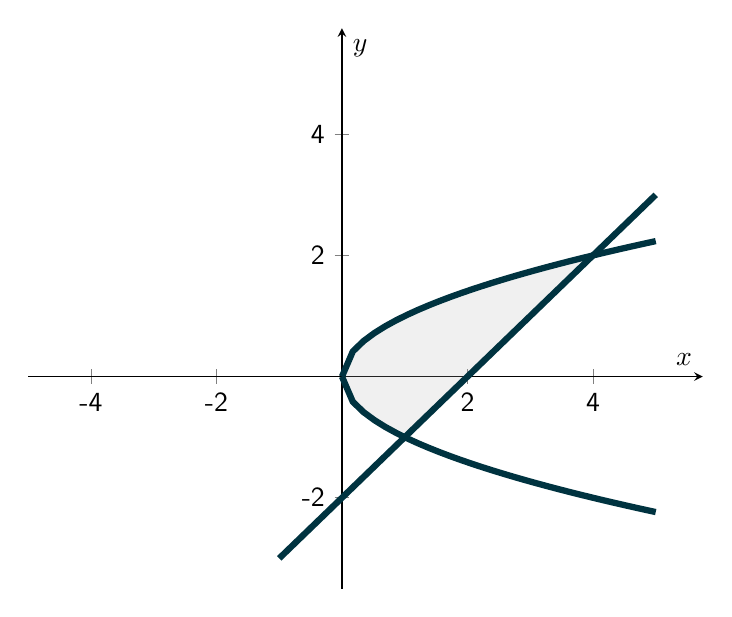
\begin{tikzpicture}[scale=1.25]
            \begin{axis}[
            axis lines = middle, very thick,
            xlabel = {$x$},
            ylabel = {$y$},
            xmin=-5, xmax=5.75,
            ymin=-3.5, ymax=5.75,
            xtick={-4,-2,0,2,4},
            xticklabels={-4,-2,0,2,4},
            ytick={-2,0,2,4},
            yticklabels={-2,0,2,4}        
            ]
            % Curves
            \addplot [name path = A,-,domain = 0:5, line width=0.8mm,DarkBlue,samples = 30] {sqrt(x)} ;
            \addplot [name path = B,-,domain = 0:5, line width=0.8mm,DarkBlue,samples = 30] {-sqrt(x)} ;
            \addplot [name path = C, line width=0.8mm, samples=4, smooth,domain=0:5, DarkBlue] coordinates {(-1,-3)(5,3)};
            % Fill area between paths
            \addplot [black!30, opacity=0.2] fill between [of = A and B, soft clip={domain=0:1}];
            \addplot [black!30, opacity=0.2] fill between [of = A and C, soft clip={domain=1:4}];
            \end{axis}
        \end{tikzpicture}    
    \end{center}   
        
    Thus
    \begin{align}
        \bar y &= \frac{M_x}M = \frac1M \int_{-1}^{2}\int_{y^2}^{y+2} 12y \, dx \, dy
    \end{align} 
    Thus
    \begin{align}
        a &= -1 \\
        b &= 2 \\
        c&= y^2 \\
        d&= y+2 \\
        f(x,y) &= \delta y = 12y
    \end{align}
    }
   \else

   \fi
    
\fi

\ifnum \Version=7
% SHORT SPHERICAL AND CYLINDRICAL EXERCISE
\part Point $P$ has rectangular (Cartesian) coordinates $(x,y,z) = (-6,0,8)$ in $\mathbb R^3$. In cylindrical coordinates, the point is $(r,\theta,z)$, and in spherical coordinates the point is $(\rho, \phi, \theta)$. Where $r=\framebox{\strut\hspace{1cm}}$, $\theta=\framebox{\strut\hspace{2cm}}$, $z=\framebox{\strut\hspace{1cm}}$, $\rho=\framebox{\strut\hspace{2cm}}$, and $\phi=\framebox{\strut\hspace{3cm}}$. 

    \ifnum \Solutions=1 {\color{DarkBlue} \textit{Solutions:} To convert to cylindrical we can use the equation $r^2 = x^2 + y^2$. 
    \begin{align}
        r^2 &= x^2 + y^2 = (-6)^2 + 0^2 = 36 \ \Rightarrow \ r = 6
    \end{align}
    To determine $\theta$ we can use $\tan\theta = y/x$. 
    \begin{align}
        \tan \theta &= \frac{y}{x} = \frac{0}{-6} = 0  \\
        \theta &= \arctan 0 
    \end{align} 
    The point in cylindrical is: 
    \begin{align}
        (r,\theta,z) &= (6,\pi,8) \\
        r &= 6 \\
        \theta &= \pi \\
        z &= 8
    \end{align}
    In spherical, we can start by obtaining $\rho$. 
    \begin{align}
        \rho^2 &= x^2+y^2+z^2\\
        \rho^2 &= (-6)^2 + 0^2 + 8^2 = 36+64 = 100 \\
        \rho &= 10
    \end{align}
    To obtain $\phi$ we can use the equation that relates $x$ to spherical. Using the expression for $x$, and the values that we already have for $x$, $\rho$ and $\theta$:
    \begin{align}
        x &= \rho \sin\phi \cos\theta \\
        -6 &= 10\sin\phi \cos(\pi) \\
        \sin\phi &= \frac{-6}{10 \cos(\pi)}  = \frac{6}{10}\\
        \phi &= \arcsin (6/10)
    \end{align}
    Our coordinates in spherical are
    \begin{align}
        \rho &= 10\\
        \phi &= \arcsin (6/10)\\
        \theta &= \pi
    \end{align}
    Note the following.
    \begin{itemize}
        \item We can, for this exercise, leave un-evaluated trig functions in the answer, because the question didn't specify that you should simplify your answer as much as possible. So it would be ok to leave your answer for $\theta$ as $\arctan 0$ or $\tan^{-1} 0$. 
        \item Our particular textbook uses the convention $(\rho, \phi, \theta)$, not $(\rho, \theta,\phi)$.
    \end{itemize}
    } 
    \else
      
    \fi
    
\fi





\ifnum \Version=8
% SHORT SPHERICAL AND CYLINDRICAL EXERCISE
\part Point $P$ has rectangular (Cartesian) coordinates $(x,y,z) = (4,4,7)$ in $\mathbb R^3$. In cylindrical coordinates, the point is $(r,\theta,z)$, and in spherical coordinates the point is $(\rho, \phi, \theta)$. Where $r=\framebox{\strut\hspace{1cm}}$, $\theta=\framebox{\strut\hspace{2cm}}$, $z=\framebox{\strut\hspace{1cm}}$, $\rho=\framebox{\strut\hspace{2cm}}$, and $\phi=\framebox{\strut\hspace{3cm}}$. 

    \ifnum \Solutions=1 {\color{DarkBlue} \textit{Solutions:} To convert to cylindrical we can use the equation $r^2 = x^2 + y^2$. 
    \begin{align}
        r^2 &= x^2 + y^2 = (4)^2 + 4^2 = 32 \ \Rightarrow \ r = \sqrt{32} = 4\sqrt2
    \end{align}
    It isn't necesssary to simplify to $4\sqrt2$. Then to determine $\theta$ we can use $\tan\theta = y/x$. 
    \begin{align}
        \tan \theta &= \frac{y}{x} = \frac{4}{4} = 1  \\
        \theta &= \arctan \pi/4
    \end{align} 
    The point in cylindrical is: 
    \begin{align}
        (r,\theta,z) &= (4\sqrt2,\pi/4,7) \\
        r &= 4\sqrt2 \\
        \theta &= \pi/4 \\
        z &= 7
    \end{align}
    In spherical, we can start by obtaining $\rho$. 
    \begin{align}
        \rho^2 &= x^2+y^2+z^2\\
        \rho^2 &= (4)^2 + 4^2 + 7^2 = 16+16+49 = 32+49 = 81 \\
        \rho &= 9
    \end{align}
    To obtain $\phi$ we can use the equation that relates $x$ to spherical. Using the expression for $x$, and the values that we already have for $x$, $\rho$ and $\theta$:
    \begin{align}
        x &= \rho \sin\phi \cos\theta \\
        4 &= 9\sin\phi \cos(\pi/4) \\
        \sin\phi &= \frac{4}{9 \cos(\pi/4)}  = \frac{4\sqrt2}{9}\\
        \phi &= \arcsin \left(\frac{4\sqrt2}{9}\right)
    \end{align}
    Note for $\phi$ we can also use:
    \begin{align}
        y &= \rho \sin\phi \sin\theta \\
        4 &= 9\sin\phi \sin(\pi/4) \\
        \sin\phi &= \frac{4}{9 \sin(\pi/4)}  = \frac{4\sqrt2}{9}\\
        \phi &= \arcsin \left(\frac{4\sqrt2}{9}\right)
    \end{align}    
    And we can also use:
    \begin{align}
        z &= \rho \cos\phi  \\
        7 &= 9\cos\phi  \\
        \sin\phi &= \frac{4}{9 \sin(\pi/4)}  = \frac{4\sqrt2}{9}\\
        \phi &= \arccos \left(\frac{7}{9}\right)
    \end{align}      
    Our coordinates in spherical are
    \begin{align}
        \rho &= 9\\
        \phi &= \arcsin \left(\frac{4\sqrt2}{9}\right), \ \textbf{or} \ \phi = \arccos(7/9)\\
        \theta &= \pi/4
    \end{align}
    Note the following.
    \begin{itemize}
        \item We can, for this exercise, leave un-evaluated trig functions in the answer, because the question didn't specify that you should simplify your answer as much as possible. So it would be ok to leave your answer for $\theta$ as $\arctan 1$ or $\tan^{-1} 1$. 
        \item Our particular textbook uses the convention $(\rho, \phi, \theta)$, not $(\rho, \theta,\phi)$.
    \end{itemize}
    } 
    \else
      
    \fi
    
\fi





% 15.6
% CENTROID Y-COORDINATE PARABOLA AND LINE
\ifnum \Version=9
    \part A thin plate with density $\delta=12$ is bounded in the $xy-$plane by $y=3-x^2$ and $y=1-x$. The plate has mass $M$. The $y-$coordinate of the centroid is $\bar y = M_x/M$, where $\displaystyle M_x = \int_A^B \int_C^D f(x,y) \, dy \, dx$,  and $A=\framebox{\strut\hspace{1cm}}$, $B=\framebox{\strut\hspace{1cm}}$, $C=\framebox{\strut\hspace{3cm}}$, $D=\framebox{\strut\hspace{3cm}}$, and $f(x,y) = \framebox{\strut\hspace{3cm}}$. 
    
    \ifnum \Solutions=1 
    {\color{DarkBlue}
    The region is bounded by 
    $$1-x \le y \le 3-x^2$$
    The given curves intersect when 
    \begin{align}
        1-x &= 3-x^2\\
        0 &= x^2-x-2 \\
        &= (x-2)(x+1)
    \end{align}
    The curves intersect at $x=-1,2$. Using $y=1-x$, the intersection points are $(-1,2)$ and $(2,-1)$. The region is shown below. 
    \begin{center}  
        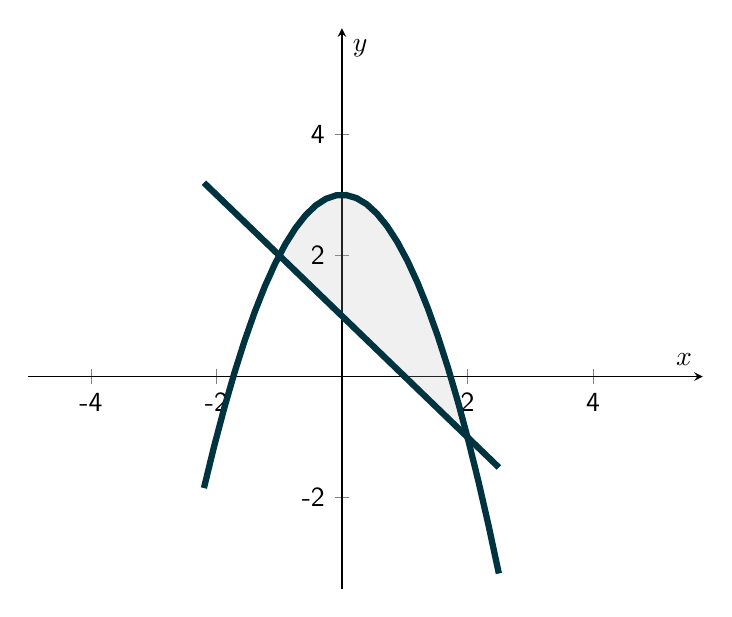
\begin{tikzpicture}[scale=1.25]
            \begin{axis}[
            axis lines = middle, very thick,
            xlabel = {$x$},
            ylabel = {$y$},
            xmin=-5, xmax=5.75,
            ymin=-3.5, ymax=5.75,
            xtick={-4,-2,0,2,4},
            xticklabels={-4,-2,0,2,4},
            ytick={-2,0,2,4},
            yticklabels={-2,0,2,4}        
            ]
            % Curves
            \addplot [name path = A,-,domain = -2.2:2.5, line width=0.8mm,DarkBlue,samples = 30] {3-x^2} ;
            \addplot [name path = C,-,domain = -2.2:2.5, line width=0.8mm,DarkBlue,samples = 4] {1-x} ;
            % Fill area between paths
            \addplot [black!30, opacity=0.2] fill between [of = A and C, soft clip={domain=-1:2}];
            \end{axis}
        \end{tikzpicture}    
    \end{center}   
        
    Thus
    \begin{align}
        \bar y &= \frac{M_x}M = \frac1M \int_{-1}^{2}\int_{1-x}^{3-x^2} 12y \, dy \, dx
    \end{align} 
    Thus
    \begin{align}
        A &= -1 \\
        B &= 2 \\
        C&= 1-x \\
        D&= 3-x^2 \\
        f(x,y) &= \delta y = 12y
    \end{align}
    }
   \else

   \fi
    
\fi
   
    % 13.3 and 13.4
% unit tangent vectors
% arc length
% curvature
% osculating circle
% unit normal

\ifnum \Version=1

\part The unit tangent vector for a curve $\mathbf r(t)$ is $\mathbf T(t) = \langle 0, \cos t, \sin t \rangle$. The unit normal vector is $\mathbf  N = \langle f(t), g(t), g(t) \rangle$, where $f(t) = \framebox{\strut\hspace{2cm}}$, $g(t) = \framebox{\strut\hspace{2cm}}$, $h(t) =\framebox{\strut\hspace{2cm}}$. 

\ifnum \Solutions=1 {\color{DarkBlue} \textit{Answer:} \textit{Solutions:} The normal vector is

\begin{align}
    \mathbf N &= \frac{d\mathbf T/dt}{|d\mathbf T/dt|} 
\end{align}
And
\begin{align}
    \mathbf T'(t) &= \langle 0,-\sin t, \cos t \rangle \\
    |\mathbf T'(t) | &= \sqrt{ 0 +(-\sin t)^2 + (\cos t)^2} =1\\
    \mathbf N &= \frac{d\mathbf T/dt}{|d\mathbf T/dt|} = \langle 0, - \sin(t),  \cos(t) \rangle
\end{align}
} 
\else
\fi        
\fi

\ifnum \Version=2

\part The velocity vector of an object moving on the curve $\mathbf r(t)$ is $\mathbf v(t) = \langle 4\cos (2t), 4\sin (2t) , 3 \rangle$ for $t>0$. The speed of the object for $t>0$ is $s(t) = |\mathbf v | = \framebox{\strut\hspace{1cm}}$. The unit tangent vector for $t>0$ is $\mathbf T = \langle f(t), g(t) , h(t) \rangle$, where $f(t) = \framebox{\strut\hspace{1.5cm}}$, $g(t) = \framebox{\strut\hspace{1.5cm}}$, $h = \framebox{\strut\hspace{1cm}}$. The curvature is $\kappa = \framebox{\strut\hspace{1cm}}$. 

\ifnum \Solutions=1 {\color{DarkBlue} \textit{Answer:} \textit{Solutions:} The speed is the magnitude of the given velocity vector and is
\begin{align}
    s &= |\mathbf v | =  \sqrt{(4\cos2t)^2 + (4\sin2t)^2 + 3^2 } = \sqrt{4^2 (\cos ^2 2 t + \sin^2 2t) + 3^2} = \sqrt{16 + 9} = 5
\end{align}
The unit tangent vector is 
\begin{align}
    \mathbf T &= \frac{\mathbf v}{|\mathbf v|} = \langle \frac{4}{5}\cos(2 t) , \frac 45 \sin (2t), \frac35 \rangle
\end{align}
For curvature we also need
\begin{align}
    \frac{d\mathbf T}{dt } &= \langle -\frac85 \sin 2t, \frac85 \cos 2t,0 \rangle \\
    \left | \frac{d\mathbf T}{dt } \right| &= \sqrt{ \left(-\frac85\sin 2t\right)^2 +   \left(\frac85 \cos 2 t\right)^2 } = \frac85
\end{align}
The curvature is
\begin{align}
    \kappa = \frac{1}{|\mathbf v |}\left| \frac{d\mathbf T}{dt}\right| = \frac{1}{5} \cdot \frac{8}{5} = \frac{8}{25}
\end{align}
} 
\else
\fi        
\fi


\ifnum \Version=3

\part A plane curve $\mathbf r(t)$ has curvature $\kappa = \frac{1}{8}$ at $\mathbf r(t_0) = \langle 15, 2 \rangle$, and the unit normal vector at $t=t_0$ is $\mathbf  N = \mathbf j = \langle 0, 1 \rangle$. The equation of the osculating circle at $t=t_0$ is \framebox{\strut\hspace{3.5cm}}.

\ifnum \Solutions=1 {\color{DarkBlue} \textit{Answer:} \textit{Solutions:} Recall that The circle of curvature, or osculating circle, at a point $P$ on a plane curve where $\kappa \ne 0$ is the circle in the plane of the curve that

\begin{enumerate}
    \item is tangent to the curve at P (has the same tangent line the curve has)
    \item has the same curvature the curve has at P
    \item lies toward the concave or inner side of the curve
\end{enumerate}
The \textbf{radius of curvature} of the curve at P is the radius of the circle of curvature, which is $\frac{1}{\kappa}$. So to obtain the radius, we calculate $\kappa$ and take the reciprocal. The \textbf{center} of the osculating circle of the curve at P lies on the inner side of the curve, and the unit normal points in the direction of the inner side of the planar curve. 

So for this problem we have a circle with radius $1/\kappa = 8$, and whose centre is 8 units away from the point $(15,2)$ in the direction of $\mathbf N$. The circle has equation
$$(x-15)^2 + (y-10)^2 = 8^2$$
} 
\else
  
\fi        
\fi




\ifnum \Version=4

\part The velocity vector for an object moving on the curve $\mathbf r(t)$ is $\mathbf v(t) = \langle t\cos t, t\sin t \rangle$. The speed of the object for $t>0$ is $s(t) = \framebox{\strut\hspace{1cm}}$. The unit tangent vector for $t>0$ is $\mathbf T = \langle f(t), g(t) \rangle$, where $f(t) = \framebox{\strut\hspace{2cm}}$, $g(t) = \framebox{\strut\hspace{2cm}}$. 

\ifnum \Solutions=1 {\color{DarkBlue} \textit{Answer:} \textit{Solutions:} The speed is the magnitude of the velocity vector and is
\begin{align}
    s &= |\mathbf v | = \sqrt{(t\cos t)^2 + (t\sin t)^2 } = \sqrt{t^2 (\cos ^2 t + \sin^2 t)} = |t|
\end{align}
But we are told that $t>0$ so we can use $|t| = t$. The unit tangent vector is 
\begin{align}
    \mathbf T &= \frac{\mathbf v}{|\mathbf v|} = \langle \cos t, \sin t \rangle
\end{align}
} 
\else
\fi        
\fi

\ifnum \Version=5

\part A plane curve $\mathbf r(t)$ has curvature $\kappa = \frac{1}{4}$ at the point $\mathbf r(t_0) = 3\mathbf i + 5\mathbf j$, and the unit normal vector at $t_0$ is $\mathbf  N = \mathbf i = \langle1,0\rangle$. The equation of the osculating circle at $t=t_0$ is \framebox{\strut\hspace{3.5cm}}.

\ifnum \Solutions=1 {\color{DarkBlue} \textit{Answer:} \textit{Solutions:} Recall that The circle of curvature, or osculating circle, at a point $P$ on a plane curve where $\kappa \ne 0$ is the circle in the plane of the curve that

\begin{enumerate}
    \item is tangent to the curve at P (has the same tangent line the curve has)
    \item has the same curvature the curve has at P
    \item lies toward the concave or inner side of the curve
\end{enumerate}
The \textbf{radius of curvature} of the curve at P is the radius of the circle of curvature, which is $\frac{1}{\kappa}$. So to obtain the radius, we calculate $\kappa$ and take the reciprocal. The \textbf{center} of the osculating circle of the curve at P lies on the inner side of the curve, and the unit normal points in the direction of the inner side of the planar curve. 

So for this problem we have a circle with radius $1/\kappa = 4$, and whose centre is 4 units away from the point $(3,5)$ in the direction of $\mathbf N$. The circle has equation
$$(x-7)^2 + (y-5)^2 = 4^2$$
} 
\else
  
\fi        
\fi


\ifnum \Version=6

\part The velocity vector for an object moving on the curve $\mathbf r(t)$ is $\mathbf v(t) = \langle 4t\cos t, 4t\sin t \rangle$ for $t>0$. The speed of the object for $t>0$ is $s(t)  = |\mathbf v | = \framebox{\strut\hspace{1cm}}$. The unit tangent vector for $t>0$ is $\mathbf T = \langle f(t), g(t) \rangle$, where $f(t) = \framebox{\strut\hspace{1.5cm}}$, $g(t) = \framebox{\strut\hspace{1.5cm}}$. The curvature is $\kappa = \framebox{\strut\hspace{1cm}}$. 

\ifnum \Solutions=1 {\color{DarkBlue} \textit{Answer:} \textit{Solutions:} The speed is the magnitude of the given velocity vector and is
\begin{align}
    s &= |\mathbf v | =  \sqrt{(4t\cos t)^2 + (4t\sin t)^2 } = \sqrt{4^2t^2 (\cos ^2 t + \sin^2 t)} = 4|t|
\end{align}
But we are told that $t>0$ so we can assume $|t| = t$. The unit tangent vector is 
\begin{align}
    \mathbf T &= \frac{\mathbf v}{|\mathbf v|} = \langle \cos t, \sin t \rangle
\end{align}
We need
\begin{align}
    \frac{d\mathbf T}{dt } &= \langle -\sin t, \cos t \rangle \\
    \left | \frac{d\mathbf T}{dt } \right| &= \sqrt{ (-\sin t)^2 +   \cos^2 t } = 1
\end{align}
The curvature is
\begin{align}
    \kappa = \frac{1}{|\mathbf v |}\left| \frac{d\mathbf T}{dt}\right| = \frac{1}{4t} 
\end{align}
} 
\else
\fi        
\fi



\ifnum \Version=7

\part The velocity vector of an object moving on the curve $\mathbf r(t)$ is $\mathbf v(t) = \langle 3\cos (2t), 3\sin (2t) \rangle$ for $t>0$. The speed of the object for $t>0$ is $s(t) = |\mathbf v | = \framebox{\strut\hspace{1.5cm}}$. The unit tangent vector for $t>0$ is $\mathbf T = \langle f(t), g(t)  \rangle$, where $f(t) = \framebox{\strut\hspace{2cm}}$, and $g(t) = \framebox{\strut\hspace{2cm}}$.  The curvature for $t>0$ is \framebox{\strut\hspace{1.5cm}}. 

\ifnum \Solutions=1 {\color{DarkBlue} \textit{Answer:} \textit{Solutions:} The speed is the magnitude of the given velocity vector and is
\begin{align}
    s &= |\mathbf v | =  \sqrt{(3\cos t)^2 + (3\sin t)^2  } = \sqrt{3^2 (\cos ^2 t + \sin^2 t) + 3^2} = \sqrt{ 9} = 3
\end{align}
The unit tangent vector is 
\begin{align}
    \mathbf T &= \frac{\mathbf v}{|\mathbf v|} 
    = \langle \frac{3}{3}\cos(2 t) , \frac 33 \sin (2t) \rangle 
    = \langle \cos(2 t) ,  \sin (2t) \rangle
\end{align}
For curvature we also need
\begin{align}
    \frac{d\mathbf T}{dt } &= \langle -2 \sin 2t, 2 \cos 2t\rangle \\
    \left | \frac{d\mathbf T}{dt } \right| &= \sqrt{ \left(-2\sin 2t\right)^2 +   \left(2 \cos 2 t\right)^2 } = 2
\end{align}
The curvature is
\begin{align}
    \kappa = \frac{1}{|\mathbf v |}\left| \frac{d\mathbf T}{dt}\right| = \frac{1}{3} \cdot 2 = \frac{2}{3}
\end{align}
} 
\else
\fi        
\fi


\ifnum \Version=8

\part A plane curve $\mathbf r(t)$ has curvature $\kappa = \frac{1}{4}$ at $\mathbf r(t_0) = \langle 5, 3 \rangle$, and the unit normal vector at $t=t_0$ is $\mathbf  N = \mathbf j = \langle 0, 1 \rangle$. The equation of the osculating circle at $t=t_0$ is \framebox{\strut\hspace{3.5cm}}.

\ifnum \Solutions=1 {\color{DarkBlue} \textit{Answer:} \textit{Solutions:} Recall that The circle of curvature, or osculating circle, at a point $P$ on a plane curve where $\kappa \ne 0$ is the circle in the plane of the curve that

\begin{enumerate}
    \item is tangent to the curve at P (has the same tangent line the curve has)
    \item has the same curvature the curve has at P
    \item lies toward the concave or inner side of the curve
\end{enumerate}
The \textbf{radius of curvature} of the curve at P is the radius of the circle of curvature, which is $\frac{1}{\kappa}$. So to obtain the radius, we calculate $\kappa$ and take the reciprocal. The \textbf{center} of the osculating circle of the curve at P lies on the inner side of the curve, and the unit normal points in the direction of the inner side of the planar curve. 

So for this problem we have a circle with radius $1/\kappa = 4$, and whose centre is 4 units away from the point $(5,3)$ in the direction of $\mathbf N$. The circle has equation
$$(x-5)^2 + (y-7)^2 = 4^2$$
} 
\else
  
\fi        
\fi






\ifnum \Version=9

\part The velocity vector of an object moving on the curve $\mathbf r(t)$ is $\mathbf v(t) = \langle t, 3 \rangle$ for $t>0$. The speed of the object at $t=2$ is $s(2) = |\mathbf v(2) | = \framebox{\strut\hspace{1.75cm}}$. The unit tangent vector at $t=2$ is $\mathbf T(2) = \langle c_1 ,c_2  \rangle$, where $c_1 = \framebox{\strut\hspace{1.75cm}}$, $c_2 = \framebox{\strut\hspace{1.75cm}}$. The curvature is $\framebox{\strut\hspace{1.75cm}}$. 

\ifnum \Solutions=1 {\color{DarkBlue} \textit{Answer:} \textit{Solutions:} The speed is the magnitude of the given velocity vector and is
\begin{align}
    s &= |\mathbf v | =  \sqrt{( t)^2 + (3)^2  } = \sqrt{t^2+9}\\
    s(2) &= \sqrt{2^2+9} = \sqrt{13}
\end{align}
We also need the unit tangent vector at $t=2$. 
\begin{align}
    \mathbf T (t) &= \frac{\mathbf v}{|\mathbf v|} = \frac{t\mathbf i + 3\mathbf j}{\sqrt{t^2+9}} \\
    \mathbf T (2) &= \frac{2\mathbf i + 3\mathbf j}{\sqrt{2^2+9}}  
    = \langle \frac{2}{\sqrt{13}} , \frac {3}{\sqrt{13}}  \rangle \\
    c_1 &= \frac{2}{\sqrt{13}}\\
    c_2 &= \frac{3}{\sqrt{13}}
\end{align}
The curvature is zero because the motion is along a straight line. 
\begin{align}
    \kappa = 0
\end{align}
} 
\else
\fi        
\fi

\ifnum \Version=10

\part A plane curve $\mathbf r(t)$ has curvature $\kappa = \frac{1}{10}$ at $\mathbf r(t_0) = \langle 5, 0 \rangle$, and the unit normal vector at $t=t_0$ is $\mathbf  N = \mathbf j = \langle 0, 1 \rangle$. The equation of the osculating circle at $t=t_0$ is \framebox{\strut\hspace{3.5cm}}.

\ifnum \Solutions=1 {\color{DarkBlue} \textit{Answer:} \textit{Solutions:} Recall that The circle of curvature, or osculating circle, at a point $P$ on a plane curve where $\kappa \ne 0$ is the circle in the plane of the curve that

\begin{enumerate}
    \item is tangent to the curve at P (has the same tangent line the curve has)
    \item has the same curvature the curve has at P
    \item lies toward the concave or inner side of the curve
\end{enumerate}
The \textbf{radius of curvature} of the curve at P is the radius of the circle of curvature, which is $\frac{1}{\kappa}$. So to obtain the radius, we calculate $\kappa$ and take the reciprocal. The \textbf{center} of the osculating circle of the curve at P lies on the inner side of the curve, and the unit normal points in the direction of the inner side of the planar curve. 

So for this problem we have a circle with radius $1/\kappa = 10$, and whose centre is 10 units away from the point $(5,0)$ in the direction of $\mathbf N$. The circle has equation
$$(x-5)^2 + (y-10)^2 = 10^2$$
} 
\else
  
\fi        
\fi
   
\end{parts}

\newpage \question[0.25] \ID
% CHANGE OF VARIABLE (15.8)
% OR APPLICATION (15.6)
% OR TRIPLE CARTESIAN (15.5) 

\ifnum \Version=1
% CENTROID
% BASED ON THOMAS EXERCISES, 15.6 #1
% SUFFICIENT FOR A PRACTICE EXAM
\question[6] A thin plate of density $\delta(x,y) = 12x$ is bounded by the lines $x = 0, y = x$, and the parabola $y = x^2-6$ in the first quadrant. 
\begin{parts} 
    \part Determine the mass of the plate, $M$. Please show your work. 
    \ifnum \Solutions=1 
    {\color{DarkBlue} \textit{Solutions:}
    Curves intersect when $$x = x^2-6 \quad \Rightarrow \quad 0 = x^2 - x - 6 = (x-3)(x+2)$$
    Or $x=3, -2$. We can ignore $x=-2$ because the region is the first quadrant. Curves intersect at the point $(3,3)$, and 
    \begin{align}
        0 \le y \le 3, \quad y \le x \le \sqrt{y+6}
    \end{align}
    The mass is
    \begin{align}
        M &= \int_0^3 \int_y^{\sqrt{y+6}} \delta \, dx \, dy \\
        &= \int_0^3 \int_y^{\sqrt{y+6}} 12x \, dx \, dy \\
        &= \int_0^3  \left. 6x^2 \right|_{x=y}^{x=\sqrt{y+6}} \, dy \\
        &= \int_0^3 6(y + 6 - y^2) \, dy \\
        &= \int_0^3 6y + 36 - 6y^2 \, dy \\
        &= \left. (3y^2 + 36y - 2y^3 ) \right|_0^3 \, dy \\
        &= 27 + 108 - 54 \\
        &= 81
    \end{align}
    }
    \else 
    \vspace{16cm}
    \fi
    \part Use your results from the previous part to set up an integral that can be used to determine the $x-$coordinate of the center of mass of the plate. You do not need to evaluate your integral. 
    \ifnum \Solutions=1 {\color{DarkBlue} \textit{Solutions:} the $x-$coordinate of the center of mass, $\bar x$, is
    \begin{align}
    \bar x &= \frac{M_y}{M} = \frac{1}{81} \int_0^3 \int_y^{\sqrt{y+6}} 12x^2 \, dx \, dy 
    \end{align}
    } 
    \else
      
    \fi
    \end{parts} 
\fi
    





\ifnum \Version=2
% LONGISH CHANGE OF VARIABLE
% VERBATUM FROM SPRING 2022 QUIZ
% hand written solution only
% SUFFICIENT FOR A PRACTICE EXAM
\question[6] Consider the double integral

$$I=\iint_R \frac{x+2y}{2y-x} dA$$

where $R$ is the parallelogram with vertices $(-3,1), (-1,0), (-1,2), (1,1)$. Our goal is to determine the area of the parallelogram using the transform below. 
$$u=x+2y, \qquad v = -x +2y$$ 
Please show your work for the following. 
\begin{parts} 
    \part Use the given transform to calculate the Jacobian of the transform, $J = \partial x(u,v)/\partial y(u,v)$. 
    \ifnum \Solutions=1 
    \else 
    \vspace{8 cm}
    \fi
    \part Use your results from Part (a) and the given transform to transform the double integral. You do not need to evaluate your integral. 
\end{parts} 

\ifnum \Solutions=1 {\color{DarkBlue} \textit{Solutions:} the integral after the transform is $$\displaystyle \frac14 \int_1^5\int_{-1}^3 \frac uv \, du \, dv$$
A screen capture of a hand-written solution from a previous offer of MATH 2551 is below. 
    \begin{figure}[h]
    \centering
    \includegraphics[width=16cm]{202302/Exam3/Images/ImgE3.OR.06.png}
    \end{figure}  
    
    } 
   \else
      
   \fi
    
\fi

\ifnum \Version=3
% CENTROID
% BASED ON THOMAS EXERCISES, 15.6 #1
% SUFFICIENT FOR A PRACTICE EXAM
\question[6] A thin plate with density $\delta(x,y) = 24y$ is bounded by the lines $x = 0, x=2y$, and the parabola $x=y^2$ in the first quadrant. 
\begin{parts} 
    \part Determine the mass of the plate, $M$. Please show your work. 
    
    \ifnum \Solutions=1 
    {\color{DarkBlue} \textit{Solutions:}
    Curves intersect when $$2y = y^2 \quad \Rightarrow \quad 0 = y^2-2y = y(y-2)$$
    Or $y=0,2$. Curves intersect at the points $(0,0)$, $(4,2)$. 
    The mass is
    \begin{align}
        M = \int_0^4 \int_{x/2}^{\sqrt{x}} \delta \, dy \, dx 
        &= \int_0^4 \int_{x/2}^{\sqrt{x}} 24y \, dy \, dx \\
        &= \int_0^4  \left. 12y^2 \right|_{y=x/2}^{y=\sqrt{x}} \, dx \\
        &= 12 \int_0^4 (x-\frac{x^2}{4}) \, dx \\
        &= 12 \left. (\frac{x^2}{2} - \frac{x^3}{12} ) \right|_0^4 \, dy \\
        &= 12 (\frac{16}{2} - \frac{64}{12}) \\
        &= 96 - 64\\
        &= 32
    \end{align}
    \textbf{An Alternate Solution}\\
    Another way to approach this problem is to use the integration order $dx\,dy$. In this case the double integral becomes
    \begin{align}
        M = \int_0^2 \int_{y^2}^{2y} \delta \, dx \, dy
        &= \int_0^2 \int_{y^2}^{2y} 24y \, dx \, dy \\
        &= 24\int_0^2  \left. yx \right|_{x=y^2}^{x=2y} \, dy \\
        &= 24 \int_0^2 (2y^2 - y^3) \, dy \\
        &= 24 \left. (\frac{2y^3}{3} - \frac{y^4}{4} ) \right|_0^2 \, dy \\
        &= 24 (\frac{16}{3} - \frac{16}{4}) \\
        &= \frac{24\cdot16}{3} - 24\cdot 4 \\
        &= 8\cdot16 - 96 \\
        &= 128 - 96 \\
        &= 32
    \end{align}    
    }
    \else 
    \vspace{14cm}
    \fi
    \part Use your results from the previous part to set up an integral that can be used to determine the $x-$coordinate of the center of mass of the plate. You do not need to evaluate your integral. 
    \ifnum \Solutions=1 {\color{DarkBlue} \textit{Solutions:} the $x-$coordinate of the center of mass, $\bar x$, is
    \begin{align}
    \bar x &= \frac{M_y}{M} = \frac{1}{32} \int_0^4 \int_{x/2}^{\sqrt{x}} 24xy \, dy \, dx
    \end{align}
    \textbf{An Alternate Solution}\\    
    It is also ok to use the integration order $dx\,dy$. In this case the double integral becomes
    \begin{align}
    \bar x &= \frac{M_y}{M} = \frac{1}{32} \int_0^2 \int_{y^2}^{2y} 24xy \, dx \, dy 
    \end{align}
    } 
    \else
      
    \fi
    \end{parts} 
\fi

\ifnum \Version=4
% VERSION B
% LONG CHANGE OF VARIABLE
% BASED ON AN EXAMPLE FROM THOMAS
% SECTION 15.8 FROM THOMAS
\question[6] Consider the double integral

$$I= 9 \iint_R (y-2x)^2 \sqrt{x+y} \, dA$$

where $R$ is the region in the first quadrant bounded by the lines $x=0$, $y=0$, and $y=1-x$. Our goal is to determine the area of $R$ using the transform below. 
$$u=x+y, \qquad v = y-2x$$ 
Please show your work for the following. 
\begin{parts} 
    \part Use the given transform to calculate the Jacobian of the transform, $J = \partial x(u,v)/\partial y(u,v)$. 
    \ifnum \Solutions=1 {\color{DarkBlue} \textit{Solutions:} Solving for $x$ and $y$ using an augmented matrix,
    \begin{align}
        \begin{pmatrix} 1 & 1 & u \\-2 & 1 & v\end{pmatrix} 
        \sim \begin{pmatrix} 1 & 1 & u \\0 & 3 & 2u+v\end{pmatrix} 
        \sim \begin{pmatrix} 1 & 0 & u/3 - v/3 \\0 & 1 & 2u/3+v/3 \end{pmatrix} 
    \end{align}
    Thus
    \begin{align}
        x &= \frac13(u-v), \ y = \frac13(2u+v) \\
        J(u,v) & = \begin{vmatrix} \DXDU & \DXDV \\[8pt] \DYDU & \DYDV \end{vmatrix} = \begin{vmatrix} 1/3 & -1/3 \\ 2/3 & 1/3 \end{vmatrix} = 1/9 + 2/9 = 1/3
    \end{align}
    }
    \else 
    \vspace{8 cm}
    \fi
    \part Use the given transform and your results from Part (a) to convert the double integral into a double integral over a region in the $uv-$plane. You do not need to evaluate your integral. 
    \ifnum \Solutions=1 {\color{DarkBlue} \textit{Solutions:} Converting each of the boundaries in the $xy-$plane into the $uv-$plane we obtain
        \begin{align}
            x+y &= 1 \quad \Rightarrow \quad \frac13(u-v) + \frac13(2u+v) = 1 &&\Rightarrow \quad u = 1\\
            x&=0 \quad \Rightarrow \quad \frac13(u-v) = 0 &&\Rightarrow \quad v = u\\
            y&= 0 \quad \Rightarrow \quad \frac13(2u+v) = 0 &&\Rightarrow \quad v = -2u
        \end{align}
        The region is described by either of the following relations:
        \begin{align}
            S_1: & \quad 0 \le u \le 1, \quad -2u \le v \le u \\
            S_2: & \quad -2 \le v \le 0, \quad -v/2 \le u \le 1, \ \text{and } 0 \le v \le 1, \quad v \le u \le 1
        \end{align}
        The first set of inequalities requires only a single double integral, but it is ok to set up two double integrals. If using $S_1$, we use $dv\,du$ and obtain
        \begin{align}
            I= 9 \iint_R (y-2x)^2 \sqrt{x+y} \, dA = 9 \int_0^1 \int_{-2u}^u v^2u^{1/2} \frac13 \,dv\,du
        \end{align}
        If using $S_2$, we use $du\,dv$ and obtain
        \begin{align}
            I= 9 \iint_R (y-2x)^2 \sqrt{x+y} \, dA 
            = 9 \int_{-2}^0 \int_{-v/2}^1 v^2u^{1/2} \frac13 \,du\,dv
            + 9 \int_{0}^1 \int_{v}^1 v^2u^{1/2} \frac13 \,du\,dv
        \end{align}        
        } 
       \else
          
       \fi
    \end{parts} 

    \fi



\ifnum \Version=5
    % USE FOR VERSION B
    % LONG CYLINDRICAL WITH APPLICATION TO MASS WITH VARYING DENSITY
    % FROM 15.8
    \question[6] An object $D$ lying in the first octant is bounded below by the $xy-$plane, above by the plane $z=3+4y$, and by the cylinder $x^2+y^2 = 4$. The density of the object at any point in $D$ is equal to the distance from the point to the $z$-axis.  Please show your work for the following.
    
    \begin{parts} 
    \part Use cylindrical coordinates to calculate the total of mass of the object, $M$. Please show your work. 
    
    \ifnum \Solutions=1 {\color{DarkBlue} The object is only in the first octant so $$0 \le \theta \le \pi/2$$ Using $\delta = \sqrt{x^2+y^2} = r$, the $z-$coordinate of the center of mass is computed using 
    \begin{align}
        M &= \iiint_D  \delta \, dV \\
        &= \int_0^{\pi/2} \int_0^2 \int_0^{3+4r\sin\theta}  \delta(r,\theta) \, r\, dz\,dr\,d\theta\\
        &= \int_0^{\pi/2} \int_0^2 \int_0^{3+4r\sin\theta}   r^2 \, dz\,dr\,d\theta\\
        &= \int_0^{\pi/2} \int_0^2    r^2 \, (3+4r\sin\theta) \,dr\,d\theta \\
        &= \int_0^{\pi/2} \int_0^2     \, (3r^2+4r^3\sin\theta) \,dr\,d\theta \\
        &= \int_0^{\pi/2}  \left. \, (r^3+r^4\sin\theta) \right|_{r=0}^{r=2} d\theta \\
        &= \int_0^{\pi/2}  (8 + 16\sin\theta) d\theta \\
        &=  \left. (8\theta - 16\cos\theta) \right|_0^{\pi/2} \\
        &=  (4\pi - 0) - (0 - 16) \\
        &= 4\pi + 16
    \end{align}
    
    } 
    \else
        \vspace{14cm}
    \fi
    
    \part Use your results from the previous part to set up a triple integral in cylindrical coordinates that can be used to determine the $z-$coordinate of the center of mass of the object. You do not need to evaluate your integral. 

    \ifnum \Solutions=1 {\color{DarkBlue} \textit{Solutions:} the $z-$coordinate of the center of mass, $\bar x$, is
    \begin{align}
    \bar z &= \frac{M_{xy}}{M} = \frac{1}{16\pi+16} \int_0^{\pi/2} \int_0^2 \int_0^{3+4r\sin\theta}  z \, \delta(r,\theta) \, r\, dz\,dr\,d\theta
    \end{align}
    } 
    \else
      
    \fi
    \end{parts} 
\fi


% TRANSFORM: SOLVE FOR X & Y, BOUNDARIES, EVALUATE, TRIANGLES
% VERSION A
\ifnum \Version=6
    \question[6] Consider the transform $u=x+y$ and $v=4x+5y$, and the integral $\displaystyle I = \iint_{R}  \,dxdy$. Region $R$ is the triangle in the $xy$-plane bounded by $x+y=0$, $4x+5y=0$, $6x+7y=4$. The transform maps $R$ to region $G$ in the $uv-$plane.  Please show your work for the following.

    \begin{enumerate}
        \item[a)] Solve the system, $u=x+y$ and $v=4x+5y$, for $x$ and $y$ in terms of $u$ and $v$.
            \ifnum \Solutions=1 {\color{DarkBlue} \\[12pt] 
            \textbf{Solutions:}
            We can use the expressions for $u$ and $v$ as an augmented matrix and row reduce. 
            \begin{align}
                \begin{pmatrix} 1 & 1 & u \\ 4 & 5 & v\end{pmatrix} 
                \sim \begin{pmatrix} 1 & 1 & u \\0 & 1 & v - 4u \end{pmatrix} 
                \sim \begin{pmatrix} 1 & 0 & 5u - v \\ 0 & 1 & v - 4u \end{pmatrix} 
            \end{align}
            Thus $x = 5u - v$, and $y = v - 4u$. 
            } 
            \else 
            \vspace{5cm}
            \fi
        \item[b)] Transform the boundaries of $R$ to the $uv-$plane. In other words, determine the boundaries of $G$ in terms of $u$ and $v$. 
            \ifnum \Solutions=1 {\color{DarkBlue} \\[12pt] 
            \textbf{Solutions:} the three lines are transformed below. 
            \begin{itemize}
                \item The line $x+y=0$ becomes $u=0$. 
                \item The line $4x+5y=0$ becomes $v=0$. 
                \item The line $6x+7y=4$ is: 
                \begin{align}
                    6x+7y &=4 \\
                    6\cdot(5u-v) + 7\cdot(v-4u) &= 4\\
                    30u -28u -6v+7v &=4 \\
                    v &= 4 -2u
                \end{align}
            \end{itemize}
            } 
        \else 
        \vspace{5cm}
        \fi        
            
        \item[c)] Use the given transformation and your results from parts (a) and (b) to set up a double integral that in the $uv-$plane that is equal to $I$. Do not evaluate the integral. You also do not need to calculate the Jacobian and may use that the Jacobian of the transform is $J(u,v) = 1$.
            \ifnum \Solutions=1 {\color{DarkBlue} \\[12pt] 
            \textbf{Solutions:}
            \begin{align}
                \iint_{R} \,dx\,dy
                &= \iint_{G}  \left| J(u,v) \right| \,dv\,du 
                = \int_0^2\int_{0}^{4-2u}  \left| 1 \right| \,dv\,du 
                = \int_0^2\int_{0}^{4-2u} \,dv\,du
            \end{align}
            Note the following.
            \begin{itemize}
                \item We did not need to compute the Jacobian but it is computed as follows. 
                $$J 
                = \begin{vmatrix} x_u & x_v \\ y_u & y_v \end{vmatrix} 
                = \begin{vmatrix} 5 & -1 \\ -4 & 1\end{vmatrix} 
                = 5 - 4
                = 1$$
                \item             We did not need to evaluate the integral but if we did:
            \begin{align}
                I = \int_0^2\int_{0}^{4-2u}  \left| 1 \right| \,dv\,du
                = 1 \int_0^2 (4-2u) \,du
                =  \left. 4u - u^2 \right|_0^2 
                = 4
            \end{align}
            \item It is also ok to use the other integration order: $I = \int_0^4\int_0^{2-v/2} \, du \, dv$.
            \end{itemize}
            } 
            \else 
            \fi        
    \end{enumerate}
 
\fi 



% TRANSFORM: SOLVE FOR X & Y, BOUNDARIES, EVALUATE, PARALLELOGRAM
% VERSION A
\ifnum \Version=7
    \question[6] Consider the integral $\displaystyle I = 2\iint_{R} x-4y \,dx\,dy$, where $R$ is the parallelogram in the $xy$-plane bounded by $x-4y=2$, $x-4y=1$, $3y-x=3$, $3y-x=6$. Suppose the transform $u=x-4y$ and $v=3y-x$, maps region $R$ to region $G$ in the $uv-$plane.  Please show your work for the following.

    \begin{enumerate}
        \item[a)] Solve the system, $u=x-4y$ and $v=3y-x$, for $x$ and $y$ in terms of $u$ and $v$.
            \ifnum \Solutions=1 {\color{DarkBlue} \\[12pt] 
            \textbf{Solutions:}
            We can use the expressions for $u$ and $v$ as an augmented matrix and row reduce. 
            \begin{align}
                \begin{pmatrix} 1 & -4 & u \\ -1 & 3 & v\end{pmatrix} 
                \sim \begin{pmatrix} 1 & -4 & u \\0 & -1 & v + u\end{pmatrix} 
                \sim \begin{pmatrix} 1 & 0 & -3u-4v\\0 & 1 & -u-v\end{pmatrix} 
            \end{align}
            Thus
            \begin{align}
                x &=  -3u-4v\\
                y &= -u-v
            \end{align}

            } 
            \else 
            \vspace{5cm}
            \fi
        \item[b)] Transform the boundaries of $R$ to the $uv-$plane. In other words, determine the boundaries of $G$ in terms of $u$ and $v$. 
            \ifnum \Solutions=1 {\color{DarkBlue} \\[12pt] 
            \textbf{Solutions:} the four lines are transformed below. 
            \begin{itemize}
                \item The line $x-4y=2$ becomes $u=2$. 
                \item The line $x-4y=1$ becomes $u=1$. 
                \item The line $3y-x=3$ becomes $v=3$. 
                \item The line $3y-x=6$ becomes $v=6$. 
            \end{itemize}
            } 
        \else 
        \vspace{5cm}
        \fi        
            
        \item[c)] Use the given transformation and your results from parts (a) and (b) to set up a double integral that in the $uv-$plane that is equal to $I$. Do not evaluate the integral. You also do not need to calculate the Jacobian and may use that the Jacobian of the transform is  $J(u,v) = -1$. 
            \ifnum \Solutions=1 {\color{DarkBlue} \\[12pt] 
            \textbf{Solutions:}
            \begin{align}
                \iint_{R} 2x-8y \,dx\,dy
                = \iint_{G} 2u \left| J(u,v) \right| \,du\,dv
                = \int_3^6\int_{1}^2 2u \left| -1 \right| \,du\,dv
                = \int_3^6\int_{1}^2 2u \,du\,dv
            \end{align}
            Note the following.
            \begin{itemize}
                \item We did not need to evaluate the integral, but if we did: 
                \begin{align}
                \iint_{R} 2x-8y \,dx\,dy
                &= \iint_{G} 2u \left| J(u,v) \right| \,du\,dv\\
                &= \int_3^6\int_{1}^2 2u \left| -1 \right| \,du\,dv\\
                &= \int_3^6\left. u^2 \right|_{1}^2 \,dv\\
                &= \int_3^6 3 \,dv\\
                &= 3 \cdot(6 -3) \\
                &= 9
            \end{align}
            \end{itemize}
            } 
            \else 
            \fi        
    \end{enumerate}
 
\fi 




% TRANSFORM: SOLVE FOR X & Y, BOUNDARIES, EVALUATE
% VERSION B
\ifnum \Version=8
    \question[6] Consider the transform $u=x-y$ and $v=4y-2x$, and the integral $\displaystyle I = \iint_{R} \,dxdy$, where $R$ denotes the triangle in the $xy$-plane bounded by $x-y=2$, $4y-2x=0$, $3y=2x$. The transform maps region $R$ to region $G$ in the $uv-$plane.  Please show your work for the following.

    \begin{enumerate}
        \item[a)] Solve the system, $u=x-y$ and $v=4y-2x$, for $x$ and $y$ in terms of $u$ and $v$.
            \ifnum \Solutions=1 {\color{DarkBlue} \\[12pt] 
            \textbf{Solutions:}
            We can use the expressions for $u$ and $v$ as an augmented matrix and row reduce. 
            \begin{align}
                \begin{pmatrix} 1 & -1 & u \\ -2 & 4 & v\end{pmatrix} 
                \sim \begin{pmatrix} 1 & -1 & u \\0 & 2 & v + 2u\end{pmatrix} 
                \sim \begin{pmatrix} 1 & -1 & u\\0 & 1 & u+v/2\end{pmatrix} 
                \sim \begin{pmatrix} 1 & 0 & 2u+v/2\\0 & 1 & u+v/2\end{pmatrix} 
            \end{align}
            Thus $x = 2u+v/2$, and $y = u + \frac{v}{2}$. 
            } 
            \else 
            \vspace{5cm}
            \fi
        \item[b)] Transform the boundaries of $R$ to the $uv-$plane. In other words, determine the boundaries of $G$ in terms of $u$ and $v$. 
            \ifnum \Solutions=1 {\color{DarkBlue} \\[12pt] 
            \textbf{Solutions:} the three lines are transformed below. 
            \begin{itemize}
                \item The line $x-y=2$ becomes $u=2$. 
                \item The line $4x-2y=0$ becomes $v=0$. 
                \item The line $3y=2x$ is: 
                \begin{align}
                    3\cdot \left(u+\frac{v}{2}\right) &= 2\cdot \left( 2u+v/2 \right) \\
                    3u + 3v/2 &= 4u + v \\
                    v/2 &= u \\
                    v &= 2u 
                \end{align}
            \end{itemize}
            } 
        \else 
        \vspace{5cm}
        \fi        
            
        \item[c)] Use the given transformation and your results from parts (a) and (b) to set up a double integral that in the $uv-$plane that is equal to $I$. Do not evaluate the integral. You also do not need to calculate the Jacobian and may use that the Jacobian of the transform is  $J(u,v) = \frac12$. 
            \ifnum \Solutions=1 {\color{DarkBlue} \\[12pt] 
            \textbf{Solutions:} the region is
            $$G = \{ (u,v) \in \mathbb R^2 \, | \, 0\le u \le 2, \ 0 \le v \le 2u\}$$
            or we can use
            $$G = \{ (u,v) \in \mathbb R^2 \, | \, 0\le v \le 4, \ v/2 \le u \le 4\}$$ 
            We can write the double integral as:
            \begin{align}
                \iint_{R} \,dx\,dy
                = \iint_{G}  \left| J(u,v) \right| \,dv\,du 
                = \int_0^2\int_{0}^{2u}  \left| \frac12 \right| \,dv\,du
                = \frac12 \int_0^2\int_{0}^{2u} \,dv\,du
            \end{align}
            Note the following.
            \begin{itemize}
                \item We did not need to compute the Jacobian but it is computed as follows. 
                $$J = \begin{vmatrix} x_u & x_v \\ y_u & y_v \end{vmatrix} = \begin{vmatrix} 2 & 1/2 \\ 1 & 1/2\end{vmatrix} = 1 - 1/2 = \frac12$$
                \item We didn't need to evaluate the integral but if we did: 
                \begin{align}
                \iint_{R} \,dx\,dy
                    &= \iint_{G}  \left| J(u,v) \right| \,dv\,du\\
                    &= \int_0^2\int_{0}^{2u}  \left| \frac12 \right| \,dv\,du\\
                    &= \frac12 \int_0^2\left.  v \right|_{v=0}^{v=2u} \,du\\
                    &= \frac12 \int_0^2 2u \,du\\
                    &=  \int_0^2 u \,du\\
                    &= \frac12 \left. u^2\right|_0^2 \\
                    &= 2
            \end{align}                
            \end{itemize}
            } 
            \else 
            \fi        
    \end{enumerate}
 
\fi 









% TRANSFORM: SOLVE FOR X & Y, BOUNDARIES, EVALUATE
% VERSION D 
\ifnum \Version=9
    \question[6] Consider the transform $u=x+y$ and $v=3x+4y$, and the integral $\displaystyle I = \iint_{R} x+y \,dxdy$, where $R$ denotes the triangle in the $xy$-plane bounded by $x+y=0$, $3x+4y=2$, and $2x+3y=0$. The transform maps region $R$ to region $G$ in the $uv-$plane. Please show your work for the following.

    \begin{enumerate}
        \item[a)] Solve the system, $u=x+y$ and $v=3x+4y$, for $x$ and $y$ in terms of $u$ and $v$.
            \ifnum \Solutions=1 {\color{DarkBlue} \\[12pt] 
            \textbf{Solutions:}
            We can use the expressions for $u$ and $v$ as an augmented matrix and row reduce. 
            \begin{align}
                \begin{pmatrix} 1 & 1 & u \\ 3 & 4 & v\end{pmatrix} 
                \sim \begin{pmatrix} 1 & 1 & u \\0 & 1 & v - 3u \end{pmatrix} 
                \sim \begin{pmatrix} 1 & 0 & 4u - v \\ 0 & 1 & v - 3u \end{pmatrix} 
            \end{align}
            Thus $x = 4u - v$, and $y = v - 3u$. 
            } 
            \else 
            \vspace{5cm}
            \fi
        \item[b)] Transform the boundaries of $R$ to the $uv-$plane. In other words, determine the boundaries of $G$ in terms of $u$ and $v$. 
            \ifnum \Solutions=1 {\color{DarkBlue} \\[12pt] 
            \textbf{Solutions:} the three lines are transformed below. 
            \begin{itemize}
                \item The line $x+y=0$ becomes $u=0$. 
                \item The line $3x+4y=2$ becomes $v=2$. 
                \item The line $2x+3y$ is: 
                \begin{align}
                    2x+3y &=0 \\
                    2\cdot(4u-v) + 3\cdot(v-3u) &= 0\\
                    8u -9u  - 2v+3v &=0 \\
                    v &= u
                \end{align}
            \end{itemize}
            } 
        \else 
        \vspace{5cm}
        \fi        
            
        \item[c)] Use the given transformation and your results from parts (a) and (b) to set up a double integral that in the $uv-$plane that is equal to $I$. Do not evaluate the integral. You also do not need to calculate the Jacobian and may use that the Jacobian of the transform is $J(u,v) = 1$. 
            \ifnum \Solutions=1 {\color{DarkBlue} \\[12pt] 
            \textbf{Solutions:}
            \begin{align}
                \iint_{R} x+y \,dx\,dy
                &= \iint_{G} u \left| J(u,v) \right| \,dv\,du\\
                &= \int_0^2\int_{u}^{2} u \left| 1 \right| \,dv\,du\\
                &= \int_0^2\int_{u}^{2} u  \,dv\,du
            \end{align}
            Note the following.
            \begin{itemize}
                \item We could also instead use
                \begin{align}
                    \iint_{R} x+y \,dx\,dy &= \int_0^2\int_{0}^{v} u  \,du\,dv
                \end{align}
                \item We did not need to compute the Jacobian but it is computed as follows. 
                $$J 
                = \begin{vmatrix} x_u & x_v \\ y_u & y_v \end{vmatrix} 
                = \begin{vmatrix} 4 & -1 \\ -3 & 1\end{vmatrix} 
                = 4 - (-1)(-3)
                = 1$$
                \item It wasn't necessary to compute the integral but: 
                \begin{align}
                    \iint_{R} x+y \,dx\,dy
                    &= \iint_{G} u \left| J(u,v) \right| \,dv\,du\\
                    &= \int_0^2\int_{u}^{2} u \left| 1 \right| \,dv\,du\\
                    &= \int_0^2 2u - u^2 \,du\\
                    &= \left. \left( u^2 - \frac{u^3}{3} \right)\right|_0^2 \\
                    &= 4 - 8/3\\
                    &= 4/3
                \end{align}                
            \end{itemize}
            } 
            \else 
            \fi        
    \end{enumerate}
 
\fi 



\newpage \question[0.25] \ID
% SPHERICAL OR CYLINDRICAL (14.7)


\ifnum \Version=1
% READY TO BE USED FOR PRACTICE EXAM
% SPHERICAL INTEGRATION
% VERBATUM FROM SPRING 2022 QUIZ
% OK FOR A PRACTICE EXAM
% hand written solution only
\question[6] Evaluate the triple integral $I=\displaystyle \iiint_D \frac{16\, x}{\sqrt2}  \, dV$, where $D$ is the region in the first octant bounded by $x^2+y^2+z^2=1$ and the planes $y=0$ and $x=y$. Please show your work. Hint: you may need to use the identity $2\sin ^2x = 1 - \cos(2x)$. 

\ifnum \Solutions=1 {\color{DarkBlue} \textit{Solutions:} below is a screen capture of a hand-written solution from a previous offer of MATH 2551. 
    \begin{figure}[h]
    \centering
    \includegraphics[width=16cm]{202302/Exam3/Images/ImgE3.OR.05.png}
    \end{figure}  
    
    } 
   \else
      
   \fi
    
\fi

\ifnum \Version=2
% OK FOR A PRACTICE EXAM
% NOT SO SHORT CYLINDRICAL EXERCISE
% VERBATUM FROM SPRING 2022 QUIZ
% hand written solution only
\question[6] Use cylindrical coordinates to determine the volume of the region bounded above by $z = 4-3x^2-3y^2$ and bounded below by $z = \sqrt{x^2+y^2}$. Please show your work. 

\ifnum \Solutions=1 {\color{DarkBlue} \textit{Solutions:} below is a screen capture of a hand-written solution from a previous offer of MATH 2551. 
    \begin{figure}[h]
    \centering
    \includegraphics[width=11cm]{202302/Exam3/Images/ImgE3.OR1C.png}
    \end{figure}  
    
    There are other ways to set up this particular integral, but the above is sufficient. 

    } 
   \else
      
   \fi
    
\fi






\ifnum \Version=3
% USE FOR VERSION A
% LONG SPHERICAL WITH APPLICATION TO MASS WITH VARYING DENSITY
% FROM 15.8
\question[6] An object $D$ lying in the first octant is bounded by the planes $x=0, y=0, z=0$, and the sphere $x^2+y^2 + z^2 = 4$. The density of the object at any point in $D$ is equal to the distance from the point to the origin. 

\begin{parts}
    \part Use spherical coordinates to calculate the mass of the object, $M$. Please show your work. 
    
    \ifnum \Solutions=1 {\color{DarkBlue} Using $\delta = \sqrt{x^2+y^2+z^2} = \rho$, the mass is computed using 
    \begin{align}
        M &= \int_0^{\pi/2} \int_0^{\pi/2} \int_0^2 \delta \, \rho^2\sin\phi \, d\rho\,d\phi\,d\theta \\
        &= \int_0^{\pi/2} \int_0^{\pi/2} \int_0^2 \rho^3\sin\phi \, d\rho\,d\phi\,d\theta \\
        &= \int_0^{\pi/2} \int_0^{\pi/2} \left. \frac14 \rho^4\sin\phi \right|_0^2 \, d\phi\,d\theta \\
        &= 4 \int_0^{\pi/2} \int_0^{\pi/2} \sin\phi \, d\phi\,d\theta \\
        &= 4 \int_0^{\pi/2} \left. -\cos\phi \right|_0^{\pi/2} \, d\theta \\
        &= 4 \int_0^{\pi/2}  \, d\theta \\
        &= 2\pi
    \end{align}
    
    } 
   \else
      \vspace{14cm}
   \fi    

   \part Use your results from the previous part to set up an integral in spherical coordinates that can be used to determine the $x-$coordinate of the center of mass of the object. You do not need to evaluate your integral. 
    \ifnum \Solutions=1 {\color{DarkBlue} In spherical coordinates, $$x = \rho \sin\phi \cos\theta$$and the $x-$coordinate of the center of mass, $\bar x$, is
    \begin{align}
    \bar x &= \frac{M_{yz}}{M} \\ 
    &= \frac{1}{M} \int_0^{\pi/2} \int_0^{\pi/2} \int_0^2 (\rho \sin\phi \cos\theta) \, \delta \, \rho^2\sin\phi \, d\rho\,d\phi\,d\theta \\
    &= \frac{1}{M} \int_0^{\pi/2} \int_0^{\pi/2} \int_0^2 \rho^4\sin^2\phi \cos\theta \, d\rho\,d\phi\,d\theta 
    \end{align}
    } 
    \else
      
    \fi
    \end{parts} 
 
\fi








\ifnum \Version=4
% USE FOR VERSION B
% LONG CYLINDRICAL WITH APPLICATION TO MASS WITH VARYING DENSITY
% FROM 15.8
\question[6] An object $D$ lying in the first octant is bounded by the planes $x=0, y=0, z=0$, $z=3+4x$ and the cylinder $x^2+y^2 = 4$. The density of the object at a point in $D$ is equal to the distance from the point to the $z$-axis. 

    \begin{parts} 
    \part Use cylindrical coordinates to calculate the total of mass of the object, $M$. Please show your work. 


    \ifnum \Solutions=1 {\color{DarkBlue} \textit{Solutions:} using $\delta = \sqrt{x^2+y^2} = r$, the $z-$coordinate of the center of mass is computed using 
    \begin{align}
        M &= \iiint_D  \delta \, dV \\
        &= \int_0^{\pi/2} \int_0^2 \int_0^{3+4r\cos\theta}  \delta(r,\theta) \, r\, dz\,dr\,d\theta\\
        &= \int_0^{\pi/2} \int_0^2 \int_0^{3+4r\cos\theta}   r^2 \, dz\,dr\,d\theta\\
        &= \int_0^{\pi/2} \int_0^2 \int_0^{3+4r\cos\theta}   r^2 \, dz\,dr\,d\theta \\ 
        &= \int_0^{\pi/2} \int_0^2    r^2 \, (3+4r\cos\theta) \,dr\,d\theta \\
        &= \int_0^{\pi/2} \int_0^2     \, (3r^2+4r^3\cos\theta) \,dr\,d\theta \\
        &= \int_0^{\pi/2}  \left. \, (r^3+r^4\cos\theta) \right|_0^2 \, d\theta \\
        &= \int_0^{\pi/2}  (8+16\cos\theta) d\theta \\
        &=  \left. (8\theta+16\sin\theta) \right|_0^{\pi/2} \\
        &= 4\pi + 16  
    \end{align}
    
    } 
   \else
      \vspace{14cm}      
   \fi
    \part Use your results from the previous part to set up a triple integral that can be used to determine the $z-$coordinate of the center of mass of the object. You do not need to evaluate your integral. 

    \ifnum \Solutions=1 {\color{DarkBlue} \textit{Solutions:} the $z-$coordinate of the center of mass, $\bar x$, is
    \begin{align}
    \bar z &= \frac{M_{xy}}{M} \\
    &= \frac{1}{16 +4\pi} \int_0^{\pi/2} \int_0^2 \int_0^{3+4r\cos\theta}  z \, \delta(r,\theta) \, r\, dz\,dr\,d\theta
    \end{align}
    } 
    \else
      
    \fi
    \end{parts} 
    
\fi


\ifnum \Version=5
% USE FOR VERSION C
% LONG SPHERICAL WITH APPLICATION TO MASS WITH VARYING DENSITY
% FROM 15.8
\question[6] An object $D$ lies above the $xy-$plane and below the upper half of the sphere $x^2+y^2 + z^2 = 4$. The density of the object at any point in $D$ is equal to the distance from the point to the origin. 

\begin{parts}
    \part Use spherical coordinates to calculate the mass of the object, $M$. Please show your work. 
    
    \ifnum \Solutions=1 {\color{DarkBlue} Using $\delta = \sqrt{x^2+y^2+z^2} = \rho$, the mass is computed using 
    \begin{align}
        M &= \int_0^{2\pi} \int_0^{\pi/2} \int_0^2 \delta \, \rho^2\sin\phi \, d\rho\,d\phi\,d\theta \\
        &= \int_0^{2\pi} \int_0^{\pi/2} \int_0^2 \rho^3\sin\phi \, d\rho\,d\phi\,d\theta \\
        &= \int_0^{2\pi} \int_0^{\pi/2} \left. \frac14 \rho^4\sin\phi \right|_0^2 \, d\phi\,d\theta \\
        &= 4 \int_0^{2\pi} \int_0^{\pi/2} \sin\phi \, d\phi\,d\theta \\
        &= 4 \int_0^{2\pi} \left. -\cos\phi \right|_0^{\pi/2} \, d\theta \\
        &= 4 \int_0^{2\pi}  \, d\theta \\
        &= 8\pi
    \end{align}
    
    } 
   \else
      \vspace{14cm}
   \fi    

   \part Use your results from the previous part to set up an integral in spherical coordinates that can be used to determine the $x-$coordinate of the center of mass of the object. You do not need to evaluate your integral. 
   
    \ifnum \Solutions=1 {\color{DarkBlue} In spherical coordinates, $$x = \rho \sin\phi \cos\theta$$and the $x-$coordinate of the center of mass, $\bar x$, is
    \begin{align}
    \bar x &= \frac{M_{yz}}{M} \\ 
    &= \frac{1}{M} \int_0^{2\pi} \int_0^{\pi/2} \int_0^2 (\rho \sin\phi \cos\theta) \, \delta \, \rho^2\sin\phi \, d\rho\,d\phi\,d\theta \\
    &= \frac{1}{M} \int_0^{2\pi} \int_0^{\pi/2} \int_0^2 \rho^4\sin^2\phi \cos\theta \, d\rho\,d\phi\,d\theta 
    \end{align}
    } 
    \else
      
    \fi
    \end{parts} 

 \fi 




\ifnum \Version=6
% USE FOR VERSION B
% LONG CYLINDRICAL WITH APPLICATION TO MASS WITH VARYING DENSITY
% FROM 15.8
\question[6] An object $D$ lying in the first octant is bounded by the planes $y=x, y=0, z=0$, $z=9+8y$ and the cylinder $x^2+y^2 = 1$. The density of the object at any point in $D$ is equal to the distance from the given point to the $z$-axis. 

    \begin{parts} 
    \part Use cylindrical coordinates to calculate the total of mass of the object, $M$. Please show your work. 


    \ifnum \Solutions=1 {\color{DarkBlue} \textit{Solutions:} using $\delta = \sqrt{x^2+y^2} = r$, mass is computed using the following. 
    \begin{align}
        M &= \iiint_D  \delta \, dV \\
        &= \int_0^{\pi/4} \int_0^1 \int_0^{9+8r\sin\theta}  \delta(r,\theta) \, r\, dz\,dr\,d\theta\\
        &= \int_0^{\pi/4} \int_0^1 \int_0^{9+8r\sin\theta}   r^2 \, dz\,dr\,d\theta\\
        &= \int_0^{\pi/4} \int_0^1    r^2 \, (9+8r\sin\theta) \,dr\,d\theta \\
        &= \int_0^{\pi/4} \int_0^1     \, (9r^2+8r^3\sin\theta) \,dr\,d\theta \\
        &= \int_0^{\pi/4}  \left. \, (3r^3+2r^4\sin\theta) \right|_0^1 \, d\theta \\
        &= \int_0^{\pi/4}  (3+2\sin\theta) d\theta \\
        &=  \left. (3\theta-2\cos\theta) \right|_0^{\pi/4} \\
        &= 3\pi/4 - 2/\sqrt2  + 2
    \end{align}
    
    Note the following. 
    \begin{itemize}
        \item We could also write final answer as $M = 3\pi/4 + 2 - \sqrt2$. 
        \item We cannot use:
        \begin{align}
            M = \iiint_D  \delta \, dV 
        &= \int_0^{\pi/4}  \int_0^{9+8r\sin\theta} \int_0^1 r^2\, dr\,dz\,d\theta
        \end{align}
        In other words we can't switch the order of the innermost two integrals because the limits for $z$ use both $r$ and $\theta$. 
        \item A common error might be to use $0 \le \theta \le \pi/2$, which would give us the answer $$M = 3\pi/2 + 2 $$
        The above is not correct!         
        \item A common mistake might be to integrate with respect to the wrong variable. For example, doing something like: 
        \begin{align}
            \int_0^{\pi/4}  (3+2\sin\theta) d\theta 
            &=  \left. (3r+2\sin\theta) \right|_0^{\pi/4} 
        \end{align}     
        The above is not correct! 
    \end{itemize}
    } 
   \else
      \vspace{14cm}      
   \fi
    \part Use your results from the previous part to set up a triple integral that can be used to determine the $z-$coordinate of the center of mass of the object. You do not need to evaluate your integral. 

    \ifnum \Solutions=1 {\color{DarkBlue} \textit{Solutions:} the $z-$coordinate of the center of mass, $\bar z$, is
    \begin{align}
    \bar z 
    &= \frac{M_{xy}}{M} 
    = \frac{1}{M} \int_0^{\pi/4} \int_0^1 \int_0^{9+8r\sin\theta}  z \,  r^2\, dz\,dr\,d\theta
    \end{align}
    Note the following. 
    \begin{itemize}
        \item The limits of integration in part (b) should be identical to what was used in part (a). So if an error were made in the limits for part (a), then points should be deducted in part a. And if the limits in part (b) are the same as what were used in part (a) then no further point deductions are needed for the limits of integration. 
        \item It isn't necessary to re-state what $M$ is in this last part of the question, because it should have been found in part (a). 
    \end{itemize}    
    } 
    \else
      
    \fi
    \end{parts} 
    
\fi



\ifnum \Version=7
% USE FOR VERSION C
% LONG SPHERICAL WITH APPLICATION TO MASS WITH VARYING DENSITY
% FROM 15.8
\question[6] An object $D$ is in the shape of an ice cream cone, as it is bounded on top by the sphere $\rho =2$ and on the sides by the cone $\phi = \pi/4$. The density of the object at any point in $D$ is equal to the distance from the given point to the origin. 

\begin{parts}
    \part Use spherical coordinates to calculate the mass of the object, $M$. Please show your work. 
    
    \ifnum \Solutions=1 {\color{DarkBlue} Using $\delta = \sqrt{x^2+y^2+z^2} = \rho$, the mass is computed using 
    \begin{align}
        M &= \int_0^{2\pi} \int_0^{\pi/4} \int_0^2 \delta \, \rho^2\sin\phi \, d\rho\,d\phi\,d\theta \\
        &= \int_0^{2\pi} \int_0^{\pi/4} \int_0^2 \rho^3\sin\phi \, d\rho\,d\phi\,d\theta \\
        &= \int_0^{2\pi} \int_0^{\pi/4} \left. \frac14 \rho^4\sin\phi \right|_{\rho = 0}^{\rho = 2} \, d\phi\,d\theta \\
        &= 4 \int_0^{2\pi} \int_0^{\pi/4} \sin\phi \, d\phi\,d\theta \\
        &= 4 \int_0^{2\pi} \left. -\cos\phi \right|_0^{\pi/4} \, d\theta \\
        &= -4 \int_0^{2\pi}  \sqrt{2}/2 - 1\, d\theta \\
        &= 8\pi(1-\sqrt2/2)
    \end{align}
    % If we had used $\delta = \rho$ and $\pi/4 \le \rho \le 2$ and $0 \le \phi \le \pi/2$, we would find that 
    % \begin{align}
    %     M &= \int_0^{2\pi} \int_0^{\pi/4} \int_{\pi/4}^2 \rho \, \rho^2\sin\phi \, d\rho\,d\phi\,d\theta \\
    %     = 
    % \end{align}
    } 
   \else
      \vspace{14cm}
   \fi    

   \part Use your results from the previous part to set up an integral in spherical coordinates that can be used to determine the $z-$coordinate of the center of mass of the object. You do not need to evaluate your integral. 
   
    \ifnum \Solutions=1 {\color{DarkBlue} In spherical coordinates, $z = \rho \cos\phi$, and the $z-$coordinate of the center of mass, $\bar z$, is
    \begin{align}
    \bar z &= \frac{M_{xy}}{M} \\ 
    &= \frac{1}{M} \int_0^{2\pi} \int_0^{\pi/4} \int_0^2 (\rho \cos\phi) \, \delta \, \rho^2\sin\phi \, d\rho\,d\phi\,d\theta \\
    &= \frac{1}{M} \int_0^{2\pi} \int_0^{\pi/4} \int_0^2 \rho^4\sin\phi\cos\phi \cos\theta \, d\rho\,d\phi\,d\theta 
    \end{align}
    } 
    \else
      
    \fi
    \end{parts} 

\fi 



\ifnum \Version=8
% LONG CYLINDRICAL WITH APPLICATION TO MASS WITH VARYING DENSITY
% FROM 15.8
% MESSY ALGEBRA BUT CAN BE MADE A BIT EASIER
\question[6] An object $D$ is the right circular cylinder whose base is the cylinder $r=2\cos\theta$ in the $xy-$plane and whose top is the plane $z=15+4y$. The density of the object at any point in $D$ is equal to the distance from the given point to the $z$-axis. 

    \begin{parts} 
    \part Use cylindrical coordinates to calculate the total of mass of the object, $M$. Please show your work. 


    \ifnum \Solutions=1 {\color{DarkBlue} \textit{Solutions:} using $\delta = \sqrt{x^2+y^2} = r$, the total mass is 
    \begin{align}
        M = \iiint_D  \delta \, dV 
        &= \int_{-\pi/2}^{\pi/2} \int_0^{2\cos\theta} \int_0^{15+4r\sin\theta}   r^2 \, dz\,dr\,d\theta\\
        &= \int_{-\pi/2}^{\pi/2} \int_0^{2\cos\theta}    r^2 \, (15+4r\sin\theta) \,dr\,d\theta \\
        &= \int_{-\pi/2}^{\pi/2} \int_0^{2\cos\theta}     \, (15r^2 + 4r^3\sin\theta) \,dr\,d\theta \\
        &= \int_{-\pi/2}^{\pi/2}  \left. \, (5r^3+r^4\sin\theta) \right|_0^{2\cos\theta} \, d\theta \\
        &= \int_{-\pi/2}^{\pi/2}  (40\cos^3\theta+16\cos^4\theta \sin\theta) d\theta \\
        &= 40 \int_{-\pi/2}^{\pi/2}  \cos^3\theta \, d\theta +16 \int_{-\pi/2}^{\pi/2}\cos^4\theta \sin\theta d\theta \label{ref:cos4sin}\\
        &= 80 \int_{0}^{\pi/2}  \cos\theta(1 - \sin^2\theta ) \, d\theta  -\frac{16}{5}\cos^5\theta |_{-\pi/2}^{\pi/2} \\
\        &= 80 \int_{0}^{\pi/2}  \cos\theta \, d\theta - 80\int_{0}^{\pi/2} \cos\theta \sin^2\theta \, d\theta  + 0 \\
        &= 80  \sin\theta \huge|_{0}^{\pi/2} - \frac{80}{3} \sin^3\theta|_{0}^{\pi/2} \\
        &= 80  - \frac{80}{3} 
    \end{align}    
    Note that the second term in (\ref{ref:cos4sin}) is the integral of an odd function over a symmetric integral, so it must be zero. Also in (\ref{ref:cos4sin}) we used the idea that integrals of even functions over symmetric intervals centered on the origin can be simplified. 
    } 
   \else
      \vspace{14cm}      
   \fi
    \part Use your results from the previous part to set up a triple integral that can be used to determine the $z-$coordinate of the center of mass of the object. You do not need to evaluate your integral. 

    \ifnum \Solutions=1 {\color{DarkBlue} \textit{Solutions:} the $z-$coordinate of the center of mass, $\bar z$, is
    \begin{align}
    \bar z &= \frac{M_{xy}}{M} 
    = \frac{1}{M} \int_{-\pi/2}^{\pi/2} \int_0^{2\cos\theta} \int_0^{15+4r\sin\theta}  z \,  r^2\, dz\,dr\,d\theta
    \end{align}
    } 
    \else
      
    \fi
    \end{parts} 
    
\fi





\ifnum \Version=9
% LONG CYLINDRICAL WITH APPLICATION TO MASS WITH VARYING DENSITY
% FROM 15.8
% MESSY ALGEBRA BUT CAN BE MADE A BIT EASIER
\question[6] An object $D$ is the right circular cylinder whose base is the cylinder $r=2\cos\theta$ in the $xy-$plane and whose top is the plane $z=15+4y$. The density of the object at any point in $D$ is equal to the distance from the given point to the $z$-axis. 

    \begin{parts} 
    \part Use cylindrical coordinates to calculate the total of mass of the object, $M$. Please show your work. 


    \ifnum \Solutions=1 {\color{DarkBlue} \textit{Solutions:} using $\delta = \sqrt{x^2+y^2} = r$, the total mass is 
    \begin{align}
        M &= \iiint_D  \delta \, dV \\
        &= \int_{-\pi/2}^{\pi/2} \int_0^{2\cos\theta} \int_0^{15+4r\sin\theta}  \delta(r,\theta) \, r\, dz\,dr\,d\theta\\
        &= \int_{-\pi/2}^{\pi/2} \int_0^{2\cos\theta} \int_0^{15+4r\sin\theta}   r^2 \, dz\,dr\,d\theta\\
        &= \int_{-\pi/2}^{\pi/2} \int_0^{2\cos\theta}    r^2 \, (15+4r\sin\theta) \,dr\,d\theta \\
        &= \int_{-\pi/2}^{\pi/2} \int_0^{2\cos\theta}     \, (15r^2 + 4r^3\sin\theta) \,dr\,d\theta \\
        &= \int_{-\pi/2}^{\pi/2}  \left. \, (5r^3+r^4\sin\theta) \right|_0^{2\cos\theta} \, d\theta \\
        &= \int_{-\pi/2}^{\pi/2}  (40\cos^3\theta+16\cos^4\theta \sin\theta) d\theta \\
        &= 40 \int_{-\pi/2}^{\pi/2}  \cos^3\theta \, d\theta +16 \int_{-\pi/2}^{\pi/2}\cos^4\theta \sin\theta d\theta 
    \end{align}
    The second term is the integral of an odd function over a symmetric integral, so it must be zero. The first term is the integral of an even function over a symmetric interval, so it can be simplified.
    \begin{align}
        M 
        &= 80 \int_{0}^{\pi/2}  \cos^3\theta \, d\theta  \\
        &= 80 \int_{0}^{\pi/2}  \cos\theta(1 - 
        \sin^2\theta ) \, d\theta  \\
        &= 80 \int_{0}^{\pi/2}  \cos\theta \, d\theta - 80\int_{0}^{\pi/2} \cos\theta \sin^2\theta \, d\theta  \\
        &= 80  \sin\theta \huge|_{0}^{\pi/2} - \frac{80}{3} \sin^3\theta|_{0}^{\pi/2} \\
        &= 80  - \frac{80}{3} 
    \end{align}    

    } 
   \else
      \vspace{14cm}      
   \fi
    \part Use your results from the previous part to set up a triple integral that can be used to determine the $z-$coordinate of the center of mass of the object. You do not need to evaluate your integral. 

    \ifnum \Solutions=1 {\color{DarkBlue} \textit{Solutions:} the $z-$coordinate of the center of mass, $\bar z$, is
    \begin{align}
    \bar z &= \frac{M_{xy}}{M} 
    = \frac{1}{M} \int_{-\pi/2}^{\pi/2} \int_0^{2\cos\theta} \int_0^{15+4r\sin\theta}  z \,  r^2\, dz\,dr\,d\theta
    \end{align}
    } 
    \else
      
    \fi
    \end{parts} 
    
\fi





\ifnum \Version=12
% LONG CYLINDRICAL THAT USES MOMENT OF INERTIA
% VERBATUM FROM SPRING 2022 QUIZ
% hand written solution only
\question[6] An object $D$ is bounded by the planes $z=0$ and $z=3+4x+8y$ and the cylinder $x^2+y^2 = 2$. The density of the object at a point is equal to the distance from the point to the $z$-axis. Use cylindrical coordinates to calculate the moment of inertia of $D$ about the $z$-axis.

\ifnum \Solutions=1 {\color{DarkBlue} \textit{Solutions:} A screen capture from a hand-written solution from a previous offer of MATH 2551 is below. 
    \begin{figure}[h]
    \centering
    \includegraphics[width=12cm]{2023Spr/Exam3/Images/ImgE3.OR.07.png}
    \end{figure}  
    
    } 
   \else
      
   \fi
    
\fi
    


\end{questions}
% % SAMPLE D
% \newpage 
% \renewcommand{\Version}{4} 
% % TEST SPECIFIC INFORMATION
\ifnum \Version=1 \renewcommand{\TestName}{Year 1 MATH 2551 Exam 3 Sample A} \fi
\ifnum \Version=2 \renewcommand{\TestName}{Year 1 MATH 2551 Exam 3 Sample B} \fi
\ifnum \Version=3 \renewcommand{\TestName}{Year 1 MATH 2551 Exam 3 Sample C} \fi
\ifnum \Version=4 \renewcommand{\TestName}{Year 1 MATH 2551 Exam 3 Sample D} \fi
\ifnum \Version=5 \renewcommand{\TestName}{Year 1 MATH 2551 Exam 3 Sample E} \fi
\ifnum \Version=6 \renewcommand{\TestName}{Year 1 MATH 2551 Exam 3 Version A} \fi
\ifnum \Version=7 \renewcommand{\TestName}{Year 1 MATH 2551 Exam 3 Version B} \fi
\ifnum \Version=8 \renewcommand{\TestName}{Year 1 MATH 2551 Exam 3 Version C} \fi
\ifnum \Version=9 \renewcommand{\TestName}{Year 1 MATH 2551 Exam 3 Version D} \fi



% TITLE
\begin{center}
\ifnum \Solutions=1 {\Large {\color{DarkBlue}\textit{Solutions}}\\[6pt]}\fi
{\Large \TestName}
\end{center}

\vspace{-16pt}

\begin{center}
\textit{Work done on scratch paper will not be graded.}

\vspace{8pt}
\textbf{A Few Helpful Formulas}
\vspace{8pt}

$
\begin{array}{llllll}
    & \displaystyle x = \rho \sin\phi \cos\theta,
    & \displaystyle y = \rho \sin\phi \sin\theta,
    & \displaystyle z = \rho \cos\phi,
    & \displaystyle dV = \rho^2 \sin \phi \, d\rho \, d\phi \, d\theta,
    & \displaystyle J(u,v) = x_uy_v - y_ux_v
\end{array} 
$
\end{center}
\begin{questions}
\question[0.5] \ID

\question[7] Fill in the blanks. You do not need to show your work. 
    
\begin{parts}
    %SECTIONS 12.1 TO 12.2 (3D, vectors)



\ifnum \Version=1
\part If $P$ is the point $(2, 8, 4)$, then the distance between $P$ and the $xy$-plane is $\framebox{\strut\hspace{1cm}}$ and the distance between $P$ and the $y$-axis is $\framebox{\strut\hspace{1cm}}$. 

\ifnum \Solutions=1 {\color{DarkBlue} \textit{Answer:} the point is 4 units above the $xy$-plane, so the first distance is 4. Looking down the $y$-axis, the point is 2 units to the left of the $y$-axis and 8 units above it, so using a right-angle triangle and the Pythgorean theorem the point is $\sqrt{2^2 + 4^2} = \sqrt{20}$ units away for the $y$-axis. 
} 
\else
  
\fi
\fi


\ifnum \Version=2
\part The point on the sphere $(x-2)^2+(y-4)^2+(z-7)^2=4$ nearest to the $xy-$plane is $P=(a,b,c)$, where $a=\framebox{\strut\hspace{.8cm}}, b=\framebox{\strut\hspace{.8cm}}, c=\framebox{\strut\hspace{.8cm}}$. The radius of the sphere is $r = \framebox{\strut\hspace{.8cm}}$. 

\ifnum \Solutions=1 {\color{DarkBlue} \textit{Answer:} $a=2$, $b=4$, $c=5$, $r = 2$. \\[12pt] \textit{Solutions:} The sphere has center $(2,4,7)$ and radius $r = 2$. Because the radius is 2 and the center has $z$--coordinate $z=7$, the sphere lies above the $xy$-plane. The point on the bottom of the sphere closest to the $xy$-plane will be 2 units directly below the center. The coordinate is $(2,4,5)$, so $a=2$, $b=4$, $c=5$. 

} 
\else
  
\fi
\fi






\ifnum \Version=3
\part An equation of the plane that is perpendicular to the $x$-axis and passes through the point $P(3,4,5)$ is $\framebox{\strut\hspace{4cm}}$. 

\ifnum \Solutions=1 {\color{DarkBlue} \textit{Answer:} The plane has equation 
\begin{align}
    \vec n \cdot (\vec x - \vec x_0) & = 0
\end{align}
Where $\vec n$ is a vector normal to the plane, $\vec x_0$ is any point in the plane, and $\vec x $ is the variable vector. We can use: 
\begin{align}
    \begin{pmatrix} 1\\0 \\0 \end{pmatrix} \cdot \left( \begin{pmatrix} x\\y\\z\end{pmatrix}  - \begin{pmatrix}3\\4\\5 \end{pmatrix} \right) & = 0 \\
    x-3 &=0 \\
    x&=3
\end{align}
} 
\else
  
\fi
\fi









\ifnum \Version=4
\part The distance between the plane $x+2y+2z=2$ and the point $S(8,2,1)$ is \framebox{\strut\hspace{1cm}}. The distance between $S$ and the $yz$-plane is $\framebox{\strut\hspace{1cm}}$. 

\ifnum \Solutions=1 {\color{DarkBlue} \textit{Solutions:} A normal to the plane is $\mathbf n = \langle 1,2,2\rangle$, and $|\mathbf{n}| = \sqrt{1^2+2^2+2^2} = \sqrt{9}=3$. A point on the plane can be found by setting $y=z=0$ and solving for $x$. Doing so gives us the point $P(2,0,0)$. Then $\mathbf{PS} = \langle6,2,1\rangle$. 
\begin{align}
    d 
    = \left| \mathbf{PS} \cdot \frac{\mathbf n}{|\mathbf{n}|} \right| 
    = \frac{1}{3}\langle6,2,1\rangle \cdot \langle 1,2,2\rangle = \frac{12}{3} = 4
\end{align}
The point $S$ is 8 units away from the $yz$-plane because the point has coordinates $(8,2,1)$. So the distance between $S$ and the $yz$-plane is 8. 
}

\else

\fi
\fi

% OOOPS!! SHOULDN'T BE HERE
\ifnum \Version=5

\part The cosine of the angle between the vectors $\langle 4,0,3\rangle$  and $\langle 2,1,2\rangle$ is \framebox{\strut\hspace{1cm}}. 

\ifnum \Solutions=1 {\color{DarkBlue} \textit{Solutions:} $\displaystyle \cos\theta = \frac{\langle 4,0,3\rangle \cdot \langle 2,1,2\rangle}{\sqrt{4^2+3^2} \sqrt{2^2+2^2+1}} = \frac{8+0+6}{\sqrt{25}\cdot \sqrt9}= \frac{14}{15}$. 
}
\else
  
\fi
\fi


% OOOPS!! SHOULDN'T BE HERE
\ifnum \Version=6

\part The projection of the point $P(2,3,4)$ onto the $yz$-plane is the point $Q(c_1,c_2,c_3)$ where $c_1 = \framebox{\strut\hspace{1cm}}$, $c_2 = \framebox{\strut\hspace{1cm}}$, $c_3 = \framebox{\strut\hspace{1cm}}$.

\ifnum \Solutions=1 {\color{DarkBlue} \textit{Solutions:} the closest point on the $yz$-plane to the point $P$ will have the same $y$ and $z$ coordinates as $P$, and will have $x$-coordinate of zero. The point is $Q(0,3,4)$, so $c_1 = 0$, $c_2=3$, $c_3=4$. No need for projection formulas. 

}
\else
  
\fi
\fi







\ifnum \Version=7
\part The point on the sphere $(x-2)^2+(y-4)^2+(z-6)^2=4$ nearest to the $yz-$plane is $P=(a,b,c)$, where $a=\framebox{\strut\hspace{1cm}}, b=\framebox{\strut\hspace{1cm}}, c=\framebox{\strut\hspace{1cm}}$.

\ifnum \Solutions=1 {\color{DarkBlue} \textit{Answer:} $a=0$, $b=4$, $c=6$. \\[12pt] \textit{Solutions:} The sphere has center $(2,4,6)$ and radius $2$. Because the radius is 2 and the center has $x$--coordinate $x=2$, the sphere lies to the right of the $yz$-plane. The point on the the sphere closest to the $xy$-plane will be 2 units directly from the center. The coordinate is $(0,4,5)$, so $a=0$, $b=4$, $c=6$. 



} 
\else
  
\fi
\fi


\ifnum \Version=8 %
\part The cosine of the angle between the vectors $\langle 2,3,-6\rangle$  and $\langle 2,2,1\rangle$ is $\cos \theta = \framebox{\strut\hspace{1cm}}$. 

\ifnum \Solutions=1 {\color{DarkBlue} \textit{Answer:} $4/21$ \\[12pt] \textit{Solutions:} $\displaystyle \cos\theta = \frac{\langle 2,3,-6\rangle \cdot \langle 2,2,1\rangle}{\sqrt{2^2+3^2+6^2} \sqrt{2^2+2^2+1}} = \frac{4}{7\cdot 3}= \frac{4}{21}$. 
}
\else
  
\fi
\fi



\ifnum \Version=9

\part The midpoint of the line segment that joins points $P(1,5,2)$ and $Q(9,3,2)$ is $S(a,b,c)$, where $a=\framebox{\strut\hspace{1cm}}$, $b=\framebox{\strut\hspace{1cm}}$, $c=\framebox{\strut\hspace{1cm}}$.

\ifnum \Solutions=1 {\color{DarkBlue} \textit{Solutions:} The midpoint is found by taking the average of the corresponding coordinates of the two points. The midpoint will be the point $(5,4,2)$. The midpoint of a line was covered in Section 12.2. 
}
\else
  
\fi
\fi 


\ifnum \Version=10
\part The equation $x^2 + y^2 - 6y + z^2 + 4z = 12$ represents a sphere whose radius is $r = \framebox{\strut\hspace{1cm}}$. The center of the sphere is at the point $P(a,b,c)$ where $a = \framebox{\strut\hspace{1cm}}$, $b = \framebox{\strut\hspace{1cm}}$, c= $\framebox{\strut\hspace{1cm}}$. 

\ifnum \Solutions=1 {\color{DarkBlue} \textit{Answer:} Completing the square and rearranging like terms: 
\begin{align}
    x^2 + y^2 - 6y + z^2 + 4z &= 12 \\
    x^2 + (y^2 - 6y +9 - 9) + (z^2 + 4z + 4 - 4 )&= 12 \\
    x^2 + (y -3)^2 + (z + 2)^2 - 9 - 4 &= 12 \\
    x^2 + (y -3)^2 + (z + 2)^2 &= 25 
\end{align}
The sphere has radius 5 and is centered at the point $(0,3,-2)$. 

} 
\else
  
\fi
\fi
    % SECTION 14.2

\ifnum \Version=1
    % THOMAS 14.1
    
    \part Consider the function $\displaystyle f(x,y) =  \frac{4x}{x^2+2x+y^2}$.

    \begin{enumerate}
        \item[i)] The range of $f(x,y)$ is \framebox{\strut\hspace{2cm}}.
        \item[ii)] Evaluate the following limit, if possible. If the limit does not exist, write DNE. $$\lim_{(x,y) \to (0,0)} f(x,y) = \framebox{\strut\hspace{1cm}}$$
        \item[iii)] An example of a point where the function $f(x,y)$ is not continuous is the point $P(a,b)$ where $a = \framebox{\strut\hspace{1cm}}$, $b = \framebox{\strut\hspace{1cm}}$.         
    \end{enumerate}
    \ifnum \Solutions=1 
    
    {\color{DarkBlue} 
    Solutions for each part are as follows. 
    \begin{itemize}
        \item[\textbf{i)}:] Note that on the $x$-axis, $y=0$ and the function is
        $$f(x,0) = \frac{4x}{x^2+2x+0} = \frac{4}{x+2}$$
        So $f$ can take on any real value except zero on the $x-$axis. Can $f$ be zero? Note also that $f(x,y)$ is equal to zero for any point $(0,y)$ and $y \ne 0$.  So the range is $\mathbb R$.

        \item[\textbf{ii)}:]  To determine the limit of the function \(f(x, y) = \frac{4x}{x^2 + 2x + y^2}\) as \(x\) and \(y\) approach zero, we can consider the limit along different paths. Let's examine the limit along the \(x\)-axis (\(y = 0\)) and the \(y\)-axis (\(x = 0\)) separately.
        Along the \(x\)-axis (\(y = 0\)):
           \[ \lim_{(x,0)\to(0,0)} \frac{4x}{x^2 + 2x + 0^2} = \lim_{x\to0} \frac{4x}{x^2 + 2x} = \lim_{x\to0} \frac{4x}{x(x + 2)} = \lim_{x\to0} \frac{4}{x + 2} = \lim_{x\to0} \frac{4}{x + 2} = 2 \]
        
            Along the \(y\)-axis (\(x = 0\)):
           \[ \lim_{(0,y)\to(0,0)} \frac{4 \cdot 0}{0^2 + 2 \cdot 0 + y^2} = 0 \]
        
        Now, since the limit along the \(x\)-axis is different from the limit along the \(y\)-axis, the overall limit as \((x, y)\) approaches \((0, 0)\) does not exist. The limit depends on the direction of approach and gives different results along different paths. The answer is DNE. 

        \item[\textbf{iii)}:] Recall that a function $f(x, y)$ is continuous at the point $P(x_0 , y_0 )$ if all three of the following conditions are met. 
        \begin{enumerate}
            \item $f$ is defined at $P$. 
            \item The limit $\displaystyle \lim_{(x,y) \to (x_0,y_0)}f(x,y)$ exists. 
            \item $\displaystyle \lim_{(x,y) \to (x_0,y_0)}f(x,y) = f(x_0,y_0)$.  
        \end{enumerate}
    
        Applying this definition, we can identify a point where the function is not continuous in a few different ways. 
        \begin{itemize}
            \item We found in the previous part that the limit at the origin does not exist, so we could use $a = b = 0$. 
            \item We can also identify a point where the function is not continuous by selecting any point where the function is not defined. Our function is not defined when the denominator is zero and the numerator is non-zero. This corresponds to the set of points where     
        $$x^2+2x+y^2 = 0$$
        Any point that satisfies this relationship is sufficient. One such point is the origin, $(0,0)$. So we can use $a = b = 0$. But there are many other points we can use. 
        \end{itemize}
        
    \end{itemize}

    

    }
    \else
    
    \fi
\fi




\ifnum \Version=2
    % THOMAS 14.1
    
    \part Consider the function $f(x,y) = \sqrt{x^2+y^2 - 1}$.
    \begin{enumerate}
        \item[i)] Where is $f(x,y)$ continuous? $ \framebox{\strut\hspace{3cm}}$. 
        \item[ii)] As $(x,y) \to (1,0)$, $f(x,y) \to \framebox{\strut\hspace{1cm}}$. If the limit does not exist write DNE. 
    \end{enumerate}
    \ifnum \Solutions=1 
    
    {\color{DarkBlue} 
        
    \textbf{i)}: Recall that a function $f(x, y)$ is continuous at the point $P(x_0 , y_0 )$ if

    \begin{enumerate}
        \item $f$ is defined at $P$. 
        \item The limit $\displaystyle \lim_{(x,y) \to (x_0,y_0)}f(x,y)$ exists. 
        \item $\displaystyle \lim_{(x,y) \to (x_0,y_0)}f(x,y) = f(x_0,y_0)$.  
    \end{enumerate}

    Also, we say that function is \textbf{continuous} if it is continuous at every point of its domain. \\[6pt] 

    This particular function is continuous everywhere on its domain. Its domain is the set $x^2+y^2 \ge 1$. So we can write the answer as $$x^2+y^2 \ge 1$$
    
    \textbf{ii)}: Substituting the limit point into $f(x,y)$ gives 
    $$\sqrt{1^2+ 0^2 - 1} = 0$$
    The answer is $0$. \\[6pt]   
    \textbf{Additional Solution Note:} You might be wondering: the limit point is at the boundary of the domain, so how might that affect the limit? Because of the way a limit is defined, for the limit to exist we only need to obtain the same value along any path \textbf{in the domain }that leads to the limit point. Which it does, because $f$ is continuous. So the limit exists and is zero. 
    }
    \else
    
    \fi
\fi








\ifnum \Version=3
    % THOMAS 14.1
    
    \part Evaluate the following limits, if possible. If the limit does not exist, write DNE. 
    \begin{enumerate}
        \item[i)] Let $\displaystyle f(x,y) = \frac{x^2-2xy + y^2}{x-y}$, with $x\ne y$. As $(x,y) \to (1,1)$, $f(x,y) \to \framebox{\strut\hspace{1cm}}$. 
        \item[ii)] Let $\displaystyle g(x,y) = \cos\left(\frac{x^2+y^2}{x+y+1}\right)$. As $(x,y) \to (0,0)$, $g(x,y) \to \framebox{\strut\hspace{1cm}}$. 
    \end{enumerate}
    \ifnum \Solutions=1 
    
    {\color{DarkBlue} 
        
    \textbf{i)}: substituting the limit point into $f(x,y)$ gives an indeterminant form $0/0$. But we can factor the numerator to express in another form. 
    $$f(x,y) = \frac{x^2-2xy + y^2}{x-y} = \frac{(x-y)^2}{x-y} = \frac{x-y}{1}= x-y$$
    Substituting the limit point now gives us that $f \to 0$. 
    
    \textbf{ii)}: substituting the limit point into $g(x,y)$ gives 
    $$g(0,0) = \cos\left(\frac{0}{0+1}\right) = \cos\left(0\right) = 1$$
    }
    \else
    
    \fi
\fi


\ifnum \Version=4
    % THOMAS 14.1
    
    \part Evaluate the following limits, if possible. If the limit does not exist, write DNE. 
    \begin{enumerate}
        \item[i)] Let $\displaystyle f(x,y) = \frac{x^2-y^2}{x-y}$, with $x\ne y$. As $(x,y) \to (1,1)$, $f(x,y) \to \framebox{\strut\hspace{1cm}}$. 
        \item[ii)] Let $\displaystyle g(x,y) = \frac{x^2+xy}{xy}$. As $(x,y) \to (0,0)$, $g(x,y) \to \framebox{\strut\hspace{1cm}}$. 
    \end{enumerate}
    \ifnum \Solutions=1 
    
    {\color{DarkBlue} 
        
    \textbf{i)}: Substituting the limit point into $f(x,y)$ gives an indeterminant form $0/0$. But we can factor the numerator to express in another form. 
    $$f(x,y) = \frac{x^2-y^2}{x-y} = \frac{(x+y)(x-y)}{x-y} = \frac{x+y}{1}= x+y$$
    Substituting the limit point now gives us that $f \to 2$. 
    
    \textbf{ii)}: Substituting the limit point into $g(x,y)$ gives an indeterminant form $0/0$. But we can consider linear paths that pass through the limit point, $y=kx$, with $k\in \mathbb R$. Our limit becomes
    $$g(x,y=kx) = \frac{x^2+x(kx)}{x(kx)} = \frac{x^2(1+k)}{kx^2} = \frac{1+k}{k} = \frac1k + 1$$
    The value of the limit depends on $k$, so the limit does not exist. The answer is DNE. 
    }
    \else
    
    \fi
\fi




\ifnum \Version=5
    % THOMAS 14.1
    
    \part Evaluate the following limits, if possible. If the limit does not exist, write DNE.
    \begin{enumerate} 
        \item[i)] Let $\displaystyle f(x,y) = \frac{x+y-9}{\sqrt{x+y}-3}$, with $x\ne y$. As $(x,y) \to (3,6)$, $f(x,y) \to \framebox{\strut\hspace{1cm}}$. 
        \item[ii)] Let $\displaystyle g(x,y) = \frac{x^4}{x^4+y^2}$. As $(x,y) \to (0,0)$, $g(x,y) \to \framebox{\strut\hspace{1cm}}$. 
    \end{enumerate}
    \ifnum \Solutions=1 
    
    {\color{DarkBlue} 
        
    \textbf{i)}: Substituting the limit point into $f(x,y)$ gives an indeterminant form $0/0$. But we can rationalize the denominator to express $f$ in another form. 
    \begin{align}
        f(x,y) 
        &= \frac{x+y-9}{\sqrt{x+y}-3} \\
        &= \frac{x+y-9}{\sqrt{x+y}-3}\frac{\sqrt{x+y}+3}{\sqrt{x+y}+3}\\
        &= \frac{x+y-9}{x+y-9}\frac{\sqrt{x+y}+3}{1}\\
        &= \sqrt{x+y}+3
    \end{align}
    
    Then 
    \begin{align}
        \lim_{(x,y) \to (3,6)} f(x,y) = \lim_{(x,y) \to (3,6)} \sqrt{x+y}+3 = 6
    \end{align}
    Substituting the limit point now gives us that $f \to 6$. 
    
    \textbf{ii)}: To evaluate the limit of the function \( g(x, y) = \frac{x^4}{x^4 + y^2} \) as \((x, y)\) approaches the origin \((0, 0)\), we can consider approaching along different paths. If the limit is the same along all paths, then the limit exists; otherwise, it does not.

    Let's consider two paths: along the x-axis (\(y = 0\)) and along the y-axis (\(x = 0\)).
    
    \begin{itemize}
        \item Along the x-axis (\(y = 0\)):
       \[ \lim_{{(x, y) \to (0, 0)}} \frac{x^4}{x^4 + y^2} = \lim_{{x \to 0}} \frac{x^4}{x^4} = \lim_{{x \to 0}} 1 = 1 \]
       \item Along the y-axis (\(x = 0\)):
       \[ \lim_{{(x, y) \to (0, 0)}} \frac{x^4}{x^4 + y^2} = \lim_{{y \to 0}} \frac{0}{y^2} = 0 \]
    \end{itemize}

    Since the limits along different paths are not the same, the limit of \( g(x, y) \) as \((x, y)\) approaches the origin does not exist. The answer is DNE. 
    }
    \else
    
    \fi
\fi





\ifnum \Version=6
    % THOMAS 14.1
    
    \part Evaluate the following limits, if possible. If the limit does not exist, write DNE. 
    \begin{enumerate}
        \item[i)] Let $\displaystyle f(x,y) = \frac{x+y}{x}$. As $(x,y) \to (0,0)$, $f(x,y) \to \framebox{\strut\hspace{1cm}}$. 
        \item[ii)] Let $\displaystyle g(x,y) = \cos\left(\frac{x^2+y^2}{x+y+1}\right)$. As $(x,y) \to (0,0)$, $g(x,y) \to \framebox{\strut\hspace{1cm}}$. 
    \end{enumerate}
    \ifnum \Solutions=1 
    
    {\color{DarkBlue} 
        
    \textbf{i)}: substituting the limit point into $f(x,y)$ gives an indeterminant form $0/0$. But we can consider linear paths that pass through the limit point, $y=kx$, with $k\in \mathbb R$. Our limit becomes
    $$f(x,y=kx) = \frac{x+ (kx)}{x} = \frac{x(1+k)}{x} = 1+k$$
    The value of the limit depends on $k$, so the limit does not exist. The answer is DNE. 
    
    \textbf{ii)}: substituting the limit point into $g(x,y)$ gives 
    $$g(0,0) = \cos\left(\frac{0}{0+1}\right) = \cos\left(0\right) = 1$$
    }
    \else
    
    \fi
\fi





\ifnum \Version=7
    % THOMAS 14.1
    
    \part Evaluate the following limits, if possible. If the limit does not exist, write DNE. 
    \begin{enumerate}
        \item[i)] Let $\displaystyle f(x,y) = \frac{x^2 + 2xy + y^2}{x+y}$, with $x+y\ne 0$. As $(x,y) \to (0,0)$, $f(x,y) \to \framebox{\strut\hspace{1cm}}$. 
        \item[ii)] Let $\displaystyle g(x,y) = \frac{x^2 - 2y}{x-y}$, with $x\ne y$. As $(x,y) \to (0,0)$, $g(x,y) \to \framebox{\strut\hspace{1cm}}$.  
    \end{enumerate}
    \ifnum \Solutions=1 
    
    {\color{DarkBlue} 
        
    \textbf{i)}: substituting the limit point into $f(x,y)$ gives an indeterminant form $0/0$. But we can factor the numerator to express in another form. 
    $$f(x,y) 
    = \frac{x^2 + 2xy + y^2}{x+y} 
    = \frac{(x+y)^2}{x+y}
    = x+y
    $$
    Substituting the limit point now gives us that $f \to 0$. 
    
    \textbf{ii)}: substituting the limit point into $g(x,y)$ gives an indeterminant form. Let's consider two paths: along the $x$-axis (\(y = 0\)) and along the $y$-axis (\(x = 0\)).
    
    \begin{itemize}
        \item Along the x-axis (\(y = 0\)):
       \[ \lim_{{(x, y) \to (0, 0)}} \frac{x^2 - 2y}{x-y} = \lim_{{x \to 0}} \frac{x^2 }{x} = \lim_{{x \to 0}} x = 0 \]
       \item Along the y-axis (\(x = 0\)):
       \[ \lim_{{(x, y) \to (0, 0)}} \frac{x^2 - 2y}{x-y} = \lim_{{y \to 0}} \frac{- 2y}{-y} = 2 \]
    \end{itemize}

    Since the limits along different paths are not the same, the limit of \( g(x, y) \) as \((x, y)\) approaches the origin does not exist. The answer is DNE. 
    }
    \else
    
    \fi
\fi


\ifnum \Version=8
    % THOMAS 14.1
    
    \part Evaluate the following limits, if possible. If the limit does not exist, write DNE. 
    \begin{enumerate}
        \item[i)] Let $\displaystyle f(x,y) = \frac{x^2 - y^2}{x-y}$, with $x-y\ne 0$. As $(x,y) \to (0,0)$, $f(x,y) \to \framebox{\strut\hspace{1cm}}$. 
        \item[ii)] Let $\displaystyle g(x,y) = \frac{x^2 - 4y}{x^2-y}$, with $x\ne y$. As $(x,y) \to (0,0)$, $g(x,y) \to \framebox{\strut\hspace{1cm}}$.  
    \end{enumerate}
    \ifnum \Solutions=1 
    
    {\color{DarkBlue} 
        
    \textbf{i)}: substituting the limit point into $f(x,y)$ gives an indeterminant form $0/0$. But we can factor the numerator to express in another form. 
    $$f(x,y) 
    = \frac{x^2 - y^2}{x-y} 
    = \frac{(x+y)(x-y)}{x-y}
    = x+y
    $$
    Substituting the limit point now gives us that $f \to 0$. 
    
    \textbf{ii)}: substituting the limit point into $g(x,y)$ gives an indeterminant form. Let's consider two paths: along the $x$-axis (\(y = 0\)) and along the $y$-axis (\(x = 0\)).
    
    \begin{itemize}
        \item Along the x-axis (\(y = 0\)):
       \[ \lim_{{(x, y) \to (0, 0)}} \frac{x^2 - 4y}{x^2-y} = \lim_{{x \to 0}} \frac{x^2 }{x^2} = \lim_{{x \to 0}} 1 = 1 \]
       \item Along the y-axis (\(x = 0\)):
       \[ \lim_{{(x, y) \to (0, 0)}} \frac{x^2 - 4y}{x^2-y} = \lim_{{y \to 0}} \frac{- 4y}{-y} = 4 \]
    \end{itemize}

    Since the limits along different paths are not the same, the limit of \( g(x, y) \) as \((x, y)\) approaches the origin does not exist. The answer is DNE. 
    }
    \else
    
    \fi
\fi






\ifnum \Version=9
    % THOMAS 14.1
    
    \part Evaluate the following limits, if possible. If the limit does not exist, write DNE. 
    \begin{enumerate}
        \item[i)] Let $\displaystyle f(x,y) = \frac{x+y-4}{\sqrt{x+y}-2}$. As $(x,y) \to (2,2)$, $f(x,y) \to \framebox{\strut\hspace{1cm}}$. 
        \item[ii)] Let $\displaystyle g(x,y) = \frac{x^4 - y^2}{x^4+y^2}$. As $(x,y) \to (0,0)$, $g(x,y) \to \framebox{\strut\hspace{1cm}}$.  
    \end{enumerate}
    \ifnum \Solutions=1 
    
    {\color{DarkBlue} 
        
    \textbf{i)}: substituting the limit point into $f(x,y)$ gives an indeterminant form $0/0$. But we can rationalize the denominator to express in another form. 
    \begin{align}
        f(x,y) 
        &= \frac{x+y-4}{\sqrt{x+y}-2} \\
        &= \frac{x+y-4}{\sqrt{x+y}-2} \cdot \frac{\sqrt{x+y}+2}{\sqrt{x+y}+2} \\
        &= \frac{x+y-4}{x+y-4} \cdot \frac{\sqrt{x+y}+2}{1} \\
        &= \sqrt{x+y}+2
    \end{align}
    Substituting the limit point now gives us that $f \to 4$. 
    
    \textbf{ii)}: substituting the limit point into $g(x,y)$ gives an indeterminant form. Let's consider two paths: along the $x$-axis (\(y = 0\)) and along the $y$-axis (\(x = 0\)).
    
    \begin{itemize}
        \item Along the $x$-axis (\(y = 0\)):
       \[ \lim_{{(x, y) \to (0, 0)}} \frac{x^4 - y^2}{x^4+y^2} = \lim_{{x \to 0}} \frac{x^4 }{x^4} = \lim_{{x \to 0}} 1 = 1 \]
       \item Along the $y$-axis (\(x = 0\)):
       \[ \lim_{{(x, y) \to (0, 0)}} \frac{x^4 - y^2}{x^4+y^2} = \lim_{{y \to 0}} \frac{ - y^2}{+y^2} = -1 \]
    \end{itemize}

    Since the limits along different paths are not the same, the limit of \( g(x, y) \) as \((x, y)\) approaches the origin does not exist. The answer is DNE. 
    }
    \else
    
    \fi
\fi



\ifnum \Version=10
    % THOMAS 14.1
    
    \part Evaluate the following limits, if possible. If the limit does not exist, write DNE. 
    \begin{enumerate}
        \item[i)] Let $\displaystyle f(x,y) = \frac{x+y-4}{\sqrt{x+y}-2}$. As $(x,y) \to (2,2)$, $f(x,y) \to \framebox{\strut\hspace{1cm}}$. 
        \item[ii)] Let $\displaystyle g(x,y) = \frac{x^4 - y^2}{x^4+y^2}$. As $(x,y) \to (0,0)$, $g(x,y) \to \framebox{\strut\hspace{1cm}}$.  
    \end{enumerate}
    \ifnum \Solutions=1 
    
    {\color{DarkBlue} 
        
    \textbf{i)}: substituting the limit point into $f(x,y)$ gives an indeterminant form $0/0$. But we can rationalize the denominator to express in another form. 
    \begin{align}
        f(x,y) 
        &= \frac{x+y-4}{\sqrt{x+y}-2} \\
        &= \frac{x+y-4}{\sqrt{x+y}-2} \cdot \frac{\sqrt{x+y}+2}{\sqrt{x+y}+2} \\
        &= \frac{x+y-4}{x+y-4} \cdot \frac{\sqrt{x+y}+2}{1} \\
        &= \sqrt{x+y}+2
    \end{align}
    Substituting the limit point now gives us that $f \to 4$. 
    
    \textbf{ii)}: substituting the limit point into $g(x,y)$ gives an indeterminant form. Let's consider two paths: along the $x$-axis (\(y = 0\)) and along the $y$-axis (\(x = 0\)).
    
    \begin{itemize}
        \item Along the $x$-axis (\(y = 0\)):
       \[ \lim_{{(x, y) \to (0, 0)}} \frac{x^4 - y^2}{x^4+y^2} = \lim_{{x \to 0}} \frac{x^4 }{x^4} = \lim_{{x \to 0}} 1 = 1 \]
       \item Along the $y$-axis (\(x = 0\)):
       \[ \lim_{{(x, y) \to (0, 0)}} \frac{x^4 - y^2}{x^4+y^2} = \lim_{{y \to 0}} \frac{ - y^2}{+y^2} = -1 \]
    \end{itemize}

    Since the limits along different paths are not the same, the limit of \( g(x, y) \) as \((x, y)\) approaches the origin does not exist. The answer is DNE. 
    }
    \else
    
    \fi
\fi



\ifnum \Version=11
    % THOMAS 14.1
    
    \part Evaluate the following limits, if possible. If the limit does not exist, write DNE. 
    \begin{enumerate}
        \item[i)] Let $\displaystyle f(x,y) = \frac{x^2 - y^2}{x-y}$, with $x-y\ne 0$. As $(x,y) \to (0,0)$, $f(x,y) \to \framebox{\strut\hspace{1cm}}$. 
        \item[ii)] Let $\displaystyle g(x,y) = \frac{x^2 - 4y}{x^2-y}$, with $x\ne y$. As $(x,y) \to (0,0)$, $g(x,y) \to \framebox{\strut\hspace{1cm}}$.  
    \end{enumerate}
    \ifnum \Solutions=1 
    
    {\color{DarkBlue} 
        
    \textbf{i)}: substituting the limit point into $f(x,y)$ gives an indeterminant form $0/0$. But we can factor the numerator to express in another form. 
    $$f(x,y) 
    = \frac{x^2 - y^2}{x-y} 
    = \frac{(x+y)(x-y)}{x-y}
    = x+y
    $$
    Substituting the limit point now gives us that $f \to 0$. 
    
    \textbf{ii)}: substituting the limit point into $g(x,y)$ gives an indeterminant form. Let's consider two paths: along the $x$-axis (\(y = 0\)) and along the $y$-axis (\(x = 0\)).
    
    \begin{itemize}
        \item Along the x-axis (\(y = 0\)):
       \[ \lim_{{(x, y) \to (0, 0)}} \frac{x^2 - 4y}{x^2-y} = \lim_{{x \to 0}} \frac{x^2 }{x^2} = \lim_{{x \to 0}} 1 = 1 \]
       \item Along the y-axis (\(x = 0\)):
       \[ \lim_{{(x, y) \to (0, 0)}} \frac{x^2 - 4y}{x^2-y} = \lim_{{y \to 0}} \frac{- 4y}{-y} = 4 \]
    \end{itemize}

    Since the limits along different paths are not the same, the limit of \( g(x, y) \) as \((x, y)\) approaches the origin does not exist. The answer is DNE. 
    }
    \else
    
    \fi
\fi

    % SECTIONS 12.5
\ifnum \Version=1
\part The cosine of the angle between the planes $2x-2y-z=1$ and $x+2y+2z=2$ is \framebox{\strut\hspace{1cm}}.

\ifnum \Solutions=1 {\color{DarkBlue} \textit{Answer:} $-4/9$ \\[12pt] \textit{Solutions:} 

$$\cos \theta = \frac{\langle 2,-2,-1\rangle \cdot \langle 1,2,2\rangle}{\sqrt{2^2+2^2+1^2}\sqrt{1^2+2^2+2^2}}= \frac{-4}{9}$$

} 
\else
  
\fi
\fi

\ifnum \Version=2
\part The distance between the plane $x+4y+8z=1$ and the point $S(4,0,0)$ is \framebox{\strut\hspace{1cm}}.

\ifnum \Solutions=1 {\color{DarkBlue} \textit{Answer:} $1/3$ \\[12pt] \textit{Solutions:} A normal to the plane is $\mathbf n = \langle 1,4,8\rangle$, and $|\mathbf{n}| = \sqrt{1^2+4^2+8^2} = \sqrt{81}=9$. A point on the plane can be found by setting $y=z=0$ and solving for $x$. Doing so gives us the point $P(1,0,0)$. Then $\mathbf{PS} = \langle3,0,0\rangle$. The distance is 
\begin{align}
    d = \left| \mathbf{PS} \cdot \frac{\mathbf n}{|\mathbf{n}|} \right| = \frac{1}{9}\langle3,0,0\rangle \cdot \langle 1,4,8\rangle = \frac13.
\end{align}
} 
\else
  
\fi
\fi


\ifnum \Version=3

\part The plane that passes through $P(5,0,2)$ and contains the line $x=1+t$, $y=t$, $z=2+t$ is \framebox{\strut\hspace{4cm}}. 

\ifnum \Solutions=1 {\color{DarkBlue} \textit{Solutions:} Plane is parallel to direction vector of given line, $\mathbf  v = \langle 1,1,1\rangle$. Line contains $Q(1,0,2)$, so plane also parallel to the vector $\mathbf{PQ} = \langle 1,0,2 \rangle - \langle 5,0,2 \rangle = \langle -4,0,0 \rangle$. It would also be ok to use any scalar multiple of this. \\[12pt]Unit normal to plane is $$\mathbf n = \mathbf  v \times \mathbf {PQ} = \begin{vmatrix} i & j & k \\ 1&1&1 \\ -4&0&0\end{vmatrix} = \langle 0, -4, 4\rangle$$ So using point $P$ and $\mathbf n$, the plane has equation \begin{align}
    (0)(x-5)+(-4)(y-0) + (4)(z-2) = 0 
\end{align}which could be simplified to  $$y-z=2$$ It isn't necessary to simplify the equation further. But we could also express the answer as 
\begin{align}
    y - z + 2 = 0
\end{align}
}
\else
  
\fi
\fi


\ifnum \Version=4

\part The plane that passes through $P(5,0,2)$ and contains the line $x=1+4t$, $y=t$, $z=2+3t$ is \framebox{\strut\hspace{4cm}}. 

\ifnum \Solutions=1 {\color{DarkBlue} \textit{Solutions:} Plane is parallel to direction vector of given line, $\mathbf  v = \langle 4,1,3\rangle$. Line contains $Q(1,0,2)$, so plane also parallel to the vector $\mathbf{PQ} = \langle 1,0,2 \rangle - \langle 5,0,2 \rangle = \langle -4,0,0 \rangle$. It would also be ok to use any scalar multiple of this. \\[12pt]Unit normal to plane is $$\mathbf n = \mathbf  v \times \mathbf {PQ} = \begin{vmatrix} i & j & k \\ 4&1&3 \\ -4&0&0\end{vmatrix} = \langle 0, -12, 4\rangle$$ So using point $P$ and $\mathbf n$, the plane has equation \begin{align}
    (0)(x-5)+(-12)(y-0) + (4)(z-2) = 0 
\end{align}which could be simplified to  $$3y-z=-2$$ It isn't necessary to simplify the equation. 
}
\else
  
\fi
\fi

\ifnum \Version=5

\part The plane that passes through $P(5,0,2)$ and contains the line $x=1+4t$, $y=t$, $z=2+2t$ is \framebox{\strut\hspace{4cm}}. 

\ifnum \Solutions=1 {\color{DarkBlue} \textit{Solutions:} Plane is parallel to direction vector of given line, $\mathbf  v = \langle 4,1,2\rangle$. Line contains $Q(1,0,2)$, so plane also parallel to the vector $\mathbf{PQ} = \langle 1,0,2 \rangle - \langle 5,0,2 \rangle = \langle -4,0,0 \rangle$. It would also be ok to use any scalar multiple of this. \\[12pt]Unit normal to plane is $$\mathbf n = \mathbf  v \times \mathbf {PQ} = \begin{vmatrix} i & j & k \\ 4&1&2 \\ -4&0&0\end{vmatrix} = \langle 0, -8, 4\rangle$$ So using point $P$ and $\mathbf n$, the plane has equation \begin{align}
    (0)(x-5)+(-8)(y-0) + (4)(z-2) = 0 
\end{align}which could be simplified to  $$2y-z=-2$$ It isn't necessary to simplify the equation. 
}
\else
  
\fi
\fi




\ifnum \Version=6
\part The distance between the plane $x+4y+8z=1$ and the point $S(28,0,0)$ is \framebox{\strut\hspace{1cm}}.

\ifnum \Solutions=1 {\color{DarkBlue} \textit{Answer:} $3$ \\[12pt] \textit{Solutions:} A normal to the plane is $\mathbf n = \langle 1,4,8\rangle$, and $|\mathbf{n}| = \sqrt{1^2+4^2+8^2} = \sqrt{81}=9$. A point on the plane can be found by setting $y=z=0$ and solving for $x$. Doing so gives us the point $P(1,0,0)$. Then $\mathbf{PS} = \langle27,0,0\rangle$. The distance is 
\begin{align}
    d 
    = \left| \mathbf{PS} \cdot \frac{\mathbf n}{|\mathbf{n}|} \right| 
    = \frac{1}{9}\langle 27,0,0\rangle \cdot \langle 1,4,8\rangle = 3.
\end{align}
} 
\else
  
\fi
\fi






\ifnum \Version=7
\part The distance between the plane $x+2y+2z=2$ and the point $S(8,2,1)$ is \framebox{\strut\hspace{1cm}}. The distance between $S$ and the $yz$-plane is $\framebox{\strut\hspace{1cm}}$. 

\ifnum \Solutions=1 {\color{DarkBlue} \textit{Solutions:} A normal to the plane is $\mathbf n = \langle 1,2,2\rangle$, and $|\mathbf{n}| = \sqrt{1^2+2^2+2^2} = \sqrt{9}=3$. A point on the plane can be found by setting $y=z=0$ and solving for $x$. Doing so gives us the point $P(2,0,0)$. Then $\mathbf{PS} = \langle6,2,1\rangle$. 
\begin{align}
    d 
    = \left| \mathbf{PS} \cdot \frac{\mathbf n}{|\mathbf{n}|} \right| 
    = \frac{1}{3}\langle6,2,1\rangle \cdot \langle 1,2,2\rangle = \frac{12}{3} = 4
\end{align}
The point $S$ is 8 units away from the $yz$-plane because the point has coordinates $(8,2,1)$. So the distance between $S$ and the $yz$-plane is 8. 
}

\else

\fi
\fi




\ifnum \Version=8

\part The plane that passes through $P(0,-2,2)$ and contains the line $x=1+t$, $y=2t$, $z=2-t$ is \framebox{\strut\hspace{4cm}}. The distance between $P$ and the $xz$-plane is $\framebox{\strut\hspace{1cm}}$. 

\ifnum \Solutions=1 {\color{DarkBlue} \textit{Solutions:} The plane is parallel to direction vector of given line, $\mathbf  v = \langle 1,2,-1 \rangle$. Line contains $Q(1,0,2)$, so plane also parallel to the vector $\mathbf{PQ} = \langle 1,0,2 \rangle - \langle 0,-2,2 \rangle = \langle 1,2,0 \rangle$. It would also be ok to use any scalar multiple of this. \\[12pt]A normal to plane is 

$$\mathbf n 
= \mathbf  v \times \mathbf {PQ} 
= \begin{vmatrix} i & j & k \\ 1&2&-1 \\ 1&2&0\end{vmatrix} 
= \langle 2, -1, 0\rangle$$ 

So using point $P(0,-2,2)$ and $\mathbf n$, the plane has equation \begin{align}
    2(x-0) - (y+2) + (0)(z-2) = 0 
\end{align}
which could be simplified to $2x-y = 2$, but it isn't necessary to simplify the equation. The point $S$ is 2 units away from the $yz$-plane because the point has coordinates $(0,-2,2)$. So the distance between $S$ and the $yz$-plane is 2. 
}
\else
  
\fi
\fi

\ifnum \Version=9
\part The cosine of the angle, $\theta$, between the planes $3x+4z=1$ and $4x+3y=2$ is $\cos \theta 
 =\framebox{\strut\hspace{1cm}}$. 

\ifnum \Solutions=1 {\color{DarkBlue} \textit{Answer:} $-4/9$ \\[12pt] \textit{Solutions:} 

$$\cos \theta = \frac{\langle 3,0,4\rangle \cdot \langle 4,3,0\rangle}{\sqrt{3^2+4^2}\sqrt{3^2+4^2}}= \frac{24}{25}$$

} 
\else
  
\fi
\fi

\ifnum \Version=10

\part The plane that passes through $P(1,3,2)$ and contains the line $x=1+t$, $y=2+3t$, $z=2+2t$ is \framebox{\strut\hspace{4cm}}. The distance between the point $P$ and the $x$-axis is \framebox{\strut\hspace{1cm}}. 

\ifnum \Solutions=1 {\color{DarkBlue} \textit{Solutions:} The plane is parallel to direction vector of given line, $\mathbf  v = \langle 1,3,2\rangle$. Line contains $Q(1,2,2)$, so the plane is also parallel to the vector $\mathbf{PQ} = \langle 1,2,2 \rangle - \langle 1,3,2 \rangle = \langle 0,-1,0 \rangle$. It would also be ok to use any scalar multiple of this. \\[12pt]
A normal to the plane is $$\mathbf n = \mathbf  v \times \mathbf {PQ} = \begin{vmatrix} i & j & k \\ 1&3&2 \\ 0&-1&0\end{vmatrix} = \langle 2,0,-1\rangle = 2\mathbf i-\mathbf k$$ So using point $P(1,3,2)$ and $\mathbf n$, the plane has equation \begin{align}
    (2)(x-1)+(0)(y-3) + (-1)(z-2) = 0 
\end{align}which could be simplified to other forms, such as $$2x-z=0$$ But it isn't necessary to simplify the equation. The distance between the point and the $x$-axis is $\sqrt{3^2+2^2} = \sqrt{13}$.
}
\else
  
\fi
\fi
    %12.6 

\ifnum \Version=1 
\part Identify the surface $x^2-y+2z^2 = 4$ by type (cone, paraboloid, etc.). \framebox{\strut\hspace{3cm}}.

\ifnum \Solutions=1 {\color{DarkBlue} \textit{Answer:} elliptical paraboloid \\[12pt] \textit{Solutions:} The curve can be expressed as $y=x^2+2z^2 -4$. In the plane $x=0$ the curve is a parabola $y=2z^2-4$. In the plane $z=0$ the curve is a parabola $y=x^2-4$. Both parabolas open over the $y$-axis. It is more accurate to refer to this shape as an elliptical paraboloid, but we'll be nice and give full credit for writing paraboloid. We do this because many people refer to $y = x^2$ and $y=2x^2$ as parabolas. So, for us, it isn't necessary to indicate that the surface is an \textbf{elliptical} paraboloid. It is sufficient to refer to this surface as a paraboloid. But be careful: a hyperbolic paraboloid is not a paraboloid! Do not refer to hyperbolic paraboloid as a paraboloid. 
} 
\else
  
\fi
\fi


\ifnum \Version=2
\part Identify the surface $-x^2+y^2+4z^2 = 0$ by type (cone, paraboloid, etc.). \framebox{\strut\hspace{3cm}}.

\ifnum \Solutions=1 {\color{DarkBlue} \textit{Answer:} elliptical cone \\[12pt] \textit{Solutions:} The curve can be expressed as $x^2=y^2+4z^2$. In the plane $x=k$ for constant $k$, the curve is an ellipse with equation $y^2+4z^2=k$. The surface intersects the plane $z=0$ along two straight lines $x=\pm y$, and likewise the plane $y=0$ along the lines $z = \pm 4z$. \textit{Note that it isn't necessary to indicate that the surface is an \textbf{elliptical} cone. It is sufficient to refer to this surface as a cone. There is no such thing as a hyperbolic cone, in this course.}
} 
\else
  
\fi
\fi



\ifnum \Version=3
\part Identify the surface $x^2+2z^2 = 16+4y-y^2$ by type (cone, ellipsoid, etc.). \framebox{\strut\hspace{4.0cm}}.

\ifnum \Solutions=1 {\color{DarkBlue} \textit{Answer:} ellipsoid\\[12pt] \textit{Solutions:} Rearrange and complete the square. 
\begin{align*}
    x^2+2z^2 &= 16+4y-y^2\\
   16&= y^2-4y+ x^2+2z^2 \\
   16&= y^2-4y+4-4 + x^2+2z^2 \\
   16&= (y-2)^2 -4 + x^2+2z^2 \\
   20&= (y-2)^2 + x^2+2z^2 
\end{align*}
Not a sphere because coefficient in front of squared terms not all the same. Surface is an ellipsoid. We can refer to spheres as ellipsoids (because a sphere is a special case of an ellipsoid), but we can't refer to an ellipsoid as a sphere unless the ellipsoid is a shpere. 
} 
\else
  
\fi
\fi






\ifnum \Version=4
\part Identify the surface $y+z^2 = 1-x^2$ by type (cone, ellipsoid, etc.). \framebox{\strut\hspace{4.6cm}}.

\ifnum \Solutions=1 {\color{DarkBlue} \textit{Answer:} paraboloid. The vertex of the paraboloid is at the point $(0,1,0)$. It is ok to call this an elliptical paraboloid, because a paraboloid is a type of elliptical paraboloid. On the other hand, it is not correct to call this a hyperbolic paraboloid, because that is a very different surface! 
} 
\else
  
\fi
\fi


\ifnum \Version=5
\part Identify the surface $x-y^2-2y=4z^2 $ by type (cone, ellipsoid, etc.). \framebox{\strut\hspace{4cm}}.

\ifnum \Solutions=1 {\color{DarkBlue} \textit{Answer:} paraboloid \\[12pt] \textit{Solutions:} In the plane $x=k$ for constant $k$, the curves are ellipses.But in the plane $y=0$, we have a parabola $x = 4z^2$. So we can call this surface a paraboloid or elliptical paraboloid. It is more accurate to refer to this shape as an elliptical paraboloid, but we'll be nice and give full credit for writing paraboloid. We do this because many people refer to $y = x^2$ and $y=2x^2$ as parabolas. So, for us, it isn't necessary to indicate that the surface is an \textbf{elliptical} paraboloid. It is sufficient to refer to this surface as a paraboloid. But be careful: a hyperbolic paraboloid is not a paraboloid! Do not refer to hyperbolic paraboloid as a paraboloid.
} 
\else
  
\fi
\fi


\ifnum \Version=6
\part Identify the surface $x-y^2+z^2 = 0$ by type (cone, ellipsoid, etc.). \framebox{\strut\hspace{4.6cm}}.

\ifnum \Solutions=1 {\color{DarkBlue} \textit{Answer:} saddle, or hyperbolic paraboloid. It would not be correct to refer to this shape as a paraboloid. A paraboloid is a very different surface. 
} 
\else
  
\fi
\fi

\ifnum \Version=7
\part Identify the surface $x^2-y^2+z = 0$ by type (cone, ellipsoid, etc.). \framebox{\strut\hspace{4.6cm}}.

\ifnum \Solutions=1 {\color{DarkBlue} \textit{Answer:} saddle, or hyperbolic paraboloid. It would not be correct to refer to this shape as a paraboloid. A paraboloid is a very different surface. 
} 
\else
\fi
\fi

\ifnum \Version=8
\part Identify the surface $-x^2-y^2+z = 0$ by type (cone, ellipsoid, etc.). \framebox{\strut\hspace{4.6cm}}.

\ifnum \Solutions=1 {\color{DarkBlue} \textit{Answer:} elliptical paraboloid. 
} 
\else
  
\fi
\fi


\ifnum \Version=9
\part Identify the surface $-x^2+y-2z^2 = 0$ by type (cone, ellipsoid, etc.). \framebox{\strut\hspace{4.6cm}}.

\ifnum \Solutions=1 {\color{DarkBlue} \textit{Answer:} paraboloid, or elliptical paraboloid. 
} 
\else
  
\fi
\fi


\ifnum \Version=10
\part Identify the surface $x-5y^2-2z^2 = 0$ by type (cone, ellipsoid, etc.). \framebox{\strut\hspace{4.6cm}}.

\ifnum \Solutions=1 {\color{DarkBlue} \textit{Answer:} paraboloid, or elliptical paraboloid. 
} 
\else
  
\fi
\fi
    % QUESTIONS FOR THOMAS SECTION 14.6 
\ifnum \Version=1
% THOMAS 14.6
% FROM 2022
\part If $z=z(x,y) = x^2y$, then the differential $dz = \framebox{\strut\hspace{3cm}}$.
\ifnum \Solutions=1 {\color{DarkBlue} \\ \textit{Answer:} $dz=2xy \, dx + x^2 \, dy$ \\[12pt] \textit{Solutions:} Applying the formula for the differential of $z=f(x,y)$ we obtain $dz = \frac{\partial f}{\partial x}dx + \frac{\partial f}{\partial y}dy =  2xy \, dx + x^2 \, dy$.
} 
\else
  
\fi     
\fi


\ifnum \Version=2
% THOMAS 14.6
% FROM 2022
% 
\part The equation of the tangent plane to $z=x^2+4y^2$ at the point $P(2,-1,8)$ is \framebox{\strut\hspace{3cm}}. 

\ifnum \Solutions=1 {\color{DarkBlue} \vspace{6pt} \textit{Answer:} $4(x-2) - 8(y+1) + z-8 =0$ \\[12pt] \textit{Solutions:} Use the formula for the equation to a tangent plane, at a point $P(x_0,y_0)$, to a surface of the form $z =f(x,y)$.
\begin{align*}
    f_x(x_0,y_0) (x-x_0) + f_y(x_0,y_0) (y-y_0) - (z-z_0) &= 0 \\ 
    2x\big|_P(x-2) + 8y\big|_P(y+1) - z+8&=0\\
    2\cdot2(x-2) + 8\cdot 1(y+1) - z+8&=0\\
    4(x-2) + 8(y+1) - z+8&=0
\end{align*}
The work shown above is sufficient. But if you like you can simplify further. 
\begin{align*}
    4(x-2) - 8(y+1) - z + 8 &=0\\
    4x - 8y -8 -8 + 8 & = z\\
    4x - 8y -8 & = z
\end{align*}
} 
\else
\fi
\fi

\ifnum \Version=3
% THOMAS 14.6
% FROM 2022
% 
\part The linearization $L(x,y)$ of $z=4x^2+2y^3$ at $P(2,1)$ is \framebox{\strut\hspace{4cm}}.

\ifnum \Solutions=1 {\color{DarkBlue} \textit{Solutions:} $L(x,y) = f(2,1) + f_x(x-2) + f_y(y-1) = 18+16(x-2)+6(y-1)$. 

} 
\else
  
\fi
\fi

\ifnum \Version=4
\part The unit vector $\mathbf u = \langle a, b \rangle$ points in direction in which $f(x,y)=3y-2x^2$ decreases most rapidly at $P(1,1)$, where $a = \framebox{\strut\hspace{0.8cm}}$, $b = \framebox{\strut\hspace{0.8cm}}$.

\ifnum \Solutions=1 {\color{DarkBlue}  \textit{Solutions:} $- (\nabla f  )\big|_P = - (\langle -4x,3\rangle  ) \big|_P= \langle 4,-3\rangle$. But $\mathbf u$ is a unit vector so $$\mathbf u = \langle 4/5, -3/5\rangle$$ So $a=4/5$ and $b=-3/5$. 

} 
\else
  
\fi
\fi


\ifnum \Version=5

\part The equation of the tangent plane to the surface $z= 5 - x^2 -y^2$ at $P(2,1,0)$ is $ \framebox{\strut\hspace{3.5cm}}.$

\ifnum \Solutions=1 {\color{DarkBlue} \textit{Answer:} $z=10-4x-2y$. \\[12pt] \textit{Solutions:} Set $z =f(x,y) = 4 -x^2 - y^2$. Then
\begin{align*}
    f_x &= -2x , \ f_x(2,1) = -4\\
    f_y &= -2y , \ f_y(2,1) = -2
\end{align*}
    Use the formula for the equation to a tangent plane, at a point $P(x_0,y_0)$, to a surface of the form $z =f(x,y)$.
\begin{align*}
    (z-z_0) &= f_x(x_0,y_0) (x-x_0) + f_y(x_0,y_0) (y-y_0) \\ 
    z- 0 &=f_x(2,1)(x-2) + f_y(2,1)(y-1)\\
    z &= -4(x-2) -2(y-1) 
\end{align*}
The above is sufficient but we can simplify to $z = -4x-2y +10$.
} 
\else
  
\fi

\fi





\ifnum \Version=6 % OK BUT A LOT OF ALGEBRA? 

\part The equation of the tangent plane to $x^2-xy-y^2+z=4$ at $P(2,1,3)$ is $ \framebox{\strut\hspace{3.5cm}}.$

\ifnum \Solutions=1 {\color{DarkBlue} \textit{Solutions:} Set $z =f(x,y) = 4 -x^2+xy +y^2$. Then
\begin{align*}
    f_x &= -2x+y , \ f_x(2,1) = -3\\
    f_y &= x+2y , \ f_y(2,1) = 4
\end{align*}
    Use the formula for the equation to a tangent plane, at a point $P(x_0,y_0)$, to a surface of the form $z =f(x,y)$.
\begin{align*}
    f_x(x_0,y_0) (x-x_0) + f_y(x_0,y_0) (y-y_0) - (z-z_0) &= 0 \\ 
    f_x(2,1)(x-2) + f_y(2,1)(y-1)-(z-3) &=0 \\
    -3(x-2) + 4(y-1) - z + 3 &=0\\
    -3x + 4y -z +6-4+3 &=0 \\
    3x-4y+z&=5
\end{align*}
} 
\else
  
\fi

\fi




% QUESTIONS FOR THOMAS SECTION 14.6 
\ifnum \Version=7
% THOMAS 14.6
% FROM 2022
\part If $z(x,y) = 2xy + x$, then the differential $dz = \framebox{\strut\hspace{3cm}}$. And the equation of the tangent plane to $z$ at the point $P(1,0,1)$ is \framebox{\strut\hspace{3cm}}. 

\ifnum \Solutions=1 {\color{DarkBlue} \textit{Solutions:} there are two parts. \begin{itemize}
    \item Applying the formula for the differential of $z=f(x,y)$ we obtain $$dz = \frac{\partial f}{\partial x}dx + \frac{\partial f}{\partial y}dy =  (2y + 1) \, dx + 2x \, dy$$ 
    \item Use the formula for the equation to a tangent plane, at a point $P(x_0,y_0)$, to a surface of the form $z =f(x,y)$.
\begin{align*}
    f_x(x_0,y_0) (x-x_0) + f_y(x_0,y_0) (y-y_0) - (z-z_0) &= 0 \\ 
    (2y+1)\big|_P(x-1) + 2x\big|_P(y-0) - (z-1) &=0\\
    (x-1) + 2y - z+1&=0\\
    x+2y-z&=0
\end{align*}
Simplification not necessary. There are many other equivalent ways of expressing the plane. 
\end{itemize}
} 
\else
  
\fi     
\fi


\ifnum \Version=8
% THOMAS 14.6
% FROM 2022
% 
\part Suppose $z=2x+4y^2+xy$. Then the differential $dz = \framebox{\strut\hspace{3cm}}$. The equation of the tangent plane to $z$ at the point $P(1,0,2)$ is $\framebox{\strut\hspace{3cm}}$. 

\ifnum \Solutions=1 {\color{DarkBlue} \textit{Solutions:} there are two parts. \begin{itemize}
    \item Applying the formula for the differential of $z=f(x,y)$ we obtain $$dz = \frac{\partial f}{\partial x}dx + \frac{\partial f}{\partial y}dy =  (2 + y) \, dx + (8 y + x)\, dy$$ 
    \item Use the formula for the equation to a tangent plane, at a point $P(x_0,y_0)$, to a surface of the form $z =f(x,y)$.
\begin{align*}
    f_x(x_0,y_0) (x-x_0) + f_y(x_0,y_0) (y-y_0) - (z-z_0) &= 0 \\ 
    (2+y)\big|_P(x-1) + (8y+x)\big|_P(y-0) - (z-2) &=0\\
    2(x-1) + y - z+2&=0\\
    2x+y-z&=0
\end{align*}
Simplification not necessary. There are many other equivalent ways of expressing the plane. 
\end{itemize}
} 
\else
  
\fi     
\fi


\ifnum \Version=9
% THOMAS 14.6
% FROM 2022
% 
\part Suppose $z(x,y)=2x^3 + 2y^2$. Then the differential $dz = \framebox{\strut\hspace{3cm}}$. The linearization of $z(x,y)$ at $P(1,2)$ is $L(x,y) = \framebox{\strut\hspace{4cm}}$. 

\ifnum \Solutions=1 {\color{DarkBlue} \textit{Solutions:} We need the partial derivatives. 
    \begin{align}
        \DZDX & = 6x^2 \\
        \DZDY &= 4y
    \end{align}
    We can use these derivatives for both parts. 
    \begin{itemize}
    \item 
    Applying the formula for the differential of $z=f(x,y)$ we obtain 
    $$dz 
    = \frac{\partial f}{\partial x}dx + \frac{\partial f}{\partial y}dy 
    =  6x^2 \, dx + 4y\, dy
    $$ 
    \item If we let $f=z$, the linearization is 
    \begin{align}
        L(x,y) 
        &= f(1,2) + f_x(1,2)(x-1) + f_y(1,2)(y-1) \\
        &= 9+6(x-1)+8(y-2) \\
        &= 6x + 9y -14
    \end{align}
    
Simplification not necessary. There are many equivalent ways of expressing the linearization. 
\end{itemize}
} 
\else
  
\fi     
\fi




\ifnum \Version=10
% THOMAS 14.6
% FROM 2022
% 
\part Suppose $z(x,y)= x^3 + 2y^2$. Then the differential $dz = \framebox{\strut\hspace{3cm}}$. The linearization of $z(x,y)$ at $P(2,1)$ is $L(x,y) = \framebox{\strut\hspace{4cm}}$. 

\ifnum \Solutions=1 {\color{DarkBlue} \textit{Solutions:} We need the partial derivatives. 
    \begin{align}
        \DZDX & = 3x^2 \\
        \DZDY &= 4y
    \end{align}
    We can use these derivatives for both parts. 
    \begin{itemize}
    \item 
    Applying the formula for the differential of $z=f(x,y)$ we obtain 
    $$dz 
    = \frac{\partial f}{\partial x}dx + \frac{\partial f}{\partial y}dy 
    =  6x^2 \, dx + 4y\, dy
    $$ 
    \item If we let $f=z$, the linearization is 
    \begin{align}
        L(x,y) 
        &= f(2,1) + f_x(2,1)(x-1) + f_y(2,1)(y-1) \\
        &= 10+12(x-2)+4(y-1) \\
        &= 12x + 4y -16
    \end{align}
    
Simplification not necessary. There are many equivalent ways of expressing the linearization. 
\end{itemize}
} 
\else
  
\fi     
\fi




\ifnum \Version=11
% THOMAS 14.6
% FROM 2022
% 
\part Suppose $z=2x+4y^2+xy$. Then the differential $dz = \framebox{\strut\hspace{3cm}}$. The equation of the tangent plane to $z$ at the point $P(1,0,2)$ is $\framebox{\strut\hspace{3cm}}$. 

\ifnum \Solutions=1 {\color{DarkBlue} \textit{Solutions:} there are two parts. \begin{itemize}
    \item Applying the formula for the differential of $z=f(x,y)$ we obtain $$dz = \frac{\partial f}{\partial x}dx + \frac{\partial f}{\partial y}dy =  (2 + y) \, dx + (8 y + x)\, dy$$ 
    \item Use the formula for the equation to a tangent plane, at a point $P(x_0,y_0)$, to a surface of the form $z =f(x,y)$.
\begin{align*}
    f_x(x_0,y_0) (x-x_0) + f_y(x_0,y_0) (y-y_0) - (z-z_0) &= 0 \\ 
    (2+y)\big|_P(x-1) + (8y+x)\big|_P(y-0) - (z-2) &=0\\
    2(x-1) + y - z+2&=0\\
    2x+y-z&=0
\end{align*}
Simplification not necessary. There are many other equivalent ways of expressing the plane. 
\end{itemize}
} 
\else
  
\fi     
\fi
    % APPLICATIONS or CYLINDRICAL or SPHERICAL (THOMAS 15.6 OR 15.7)


\ifnum \Version=1
% SHORT SPHERICAL AND CYLINDRICAL EXERCISE
% VERBATUM FROM SPRING 2022 QUIZ
% hand written solution only
\part Point $P$ has rectangular (Cartesian) coordinates $(x,y,z) = (0,-3,4)$ in $\mathbb R^3$. In cylindrical coordinates, the point is $(r,\theta,z)$, and in spherical coordinates the point is $(\rho, \phi, \theta)$. Where $r=\framebox{\strut\hspace{1cm}}$, $\theta=\framebox{\strut\hspace{1cm}}$, $z=\framebox{\strut\hspace{1cm}}$, $\rho=\framebox{\strut\hspace{1.5cm}}$, and $\phi=\framebox{\strut\hspace{3cm}}$. 

    \ifnum \Solutions=1 {\color{DarkBlue} \textit{Solutions:} To convert to cylindrical we can use the equation $r^2 = x^2 + y^2$. 
    \begin{align}
        r^2 &= x^2 + y^2 = 0^2 + (-3)^2 = 9 \ \Rightarrow \ r = 3 
    \end{align}
    To determine $\theta$ we notice that $P$ lies on the $y-$axis and has a negative $y$ value. So $\theta = 3\pi/2$.
    $$\displaystyle (r,\theta,z) = (3,\frac{3\pi}2,4)$$
    In spherical, we can start by obtaining $\rho$. 
    \begin{align}
        \rho^2 &= x^2+y^2+z^2\\
        \rho^2 &= 0^2 + (-3)^2 + 4^2 = 25 \\
        \rho &= 5 
    \end{align}
    To obtain $\phi$ we can use the equation that relates $y$ to spherical. Using the expression for $y$, and the values that we already have for $y$, $\rho$ and $\theta$:
    \begin{align}
        y &= \rho \sin\phi \sin\theta \\
        -3 &= 5\sin\phi \sin(3\pi/2) \\
        3 &= 5\sin\phi \\
        \sin\phi &= 3/5 \\
        \phi &= \arcsin (3/5)
    \end{align}
    Our coordinates in spherical are
    \begin{align}
        \rho &= 5\\
        \phi &= \arcsin (3/5)\\
        \theta &= \frac{3\pi}2  
    \end{align}
    Note the following.
    \begin{itemize}
        \item Note that we could also obtain $\phi$ using a right-angle triangle in the $yz-$plane. 
        \item Other similar approaches can lead to other equivalent expressions for $\phi$, such as $\phi = \arctan(3/4)$.
        \item Our particular textbook uses the convention $(\rho, \phi, \theta)$, not $(\rho, \theta,\phi)$.
    \end{itemize}
    } 
    \else
      
    \fi
    
\fi

% 15.6
% BASED ON  THOMAS, 15.6 #3
% GOOD PROBLEM FOR #4, EASY
\ifnum \Version=2
    \part A thin plate of density $\delta(x,y)=2$ is bounded by $y=x-1$ and $y=5-x^2$. The plate has mass $M$, and the $y-$coordinate of the center of mass is $\bar y = M_x/M$, where $M_x = \int_a^b \int_c^d f(x,y) \, dy \, dx$,  and $b=\framebox{\strut\hspace{1.0cm}}$, $c=\framebox{\strut\hspace{2cm}}$, $d=\framebox{\strut\hspace{2cm}}$, and $f(x,y) = \framebox{\strut\hspace{2cm}}$. 

    \ifnum \Solutions=1
    {\color{DarkBlue}
    The region is bounded by 
    $$x-1 \le y \le 5-x^2$$
    The given curves intersect when 
    \begin{align}
        x-1 &= 5-x^2 \\
        0 &= x^2 +x -6 \\
        &= (x+3)(x-2)
    \end{align}
    Thus
    \begin{align}
        \bar y &= \frac{M_x}M = \frac1M \int_{-3}^{2}\int_{x-1}^{5-x^2} 2y \, dy \, dx
    \end{align} 
    The density of the plate is $\delta = 2$. Thus
    \begin{align}
        a &= -3 \\
        b &= 2 \\
        c&= x-1 \\
        d&= 5-x^2 \\
        f(x,y) &= \delta y = 2y
    \end{align}
    }
   \else
   \fi
    
\fi






% 15.6
% BASED ON  THOMAS, 15.6 Example 2
% GOOD PROBLEM FOR #3, EASY
\ifnum \Version=3
    \part $R$ is the region in the $xy-$plane bounded by $y=4x$ and the curve $y=x^2$. Then $R$ has area $M$, and the $x-$coordinate of the centroid is $\bar x = M_y/M$, where $M_y = \int_a^b \int_c^d f(x,y) \, dy \, dx$,  and $a=\framebox{\strut\hspace{1.0cm}}$, $b=\framebox{\strut\hspace{1.0cm}}$, $c=\framebox{\strut\hspace{2cm}}$, $d=\framebox{\strut\hspace{2cm}}$, and $f(x,y) = \framebox{\strut\hspace{2cm}}$. 
    
    \ifnum \Solutions=1 
    {\color{DarkBlue}
    The region is bounded by 
    $$x^2 \le y \le 4x$$
    The curves $y=x^2$ and $y=4x$ intersect at $x=0$ and $x=4$. 
    Thus
    \begin{align}
        \bar x &= \frac1M \int_{0}^{4}\int_{x^2}^{4x} x \, dy \, dx
    \end{align} 
    Thus,
    \begin{align}
        a &= 0 \\
        b &= 4 \\
        c&= x^2 \\
        d&= 4x \\
        f(x,y) &= x
    \end{align}
    }
    \newpage
   \else

   \fi
    
\fi



% 15.6
% BASED ON  THOMAS, 15.6 #3
% GOOD PROBLEM FOR #4, EASY
\ifnum \Version=4
    \part A thin plate with density $\delta=4$ is bounded in the $xy-$plane by $x=2-y$ and $x=y^2$. The plate has mass $M$, and the $y-$coordinate of the center of mass is $\bar y = M_x/M$, where $M_x = \int_a^b \int_c^d f(x,y) \, dx \, dy$,  and $a=\framebox{\strut\hspace{0.8cm}}$, $b=\framebox{\strut\hspace{0.8cm}}$, $c=\framebox{\strut\hspace{1.0cm}}$, $d=\framebox{\strut\hspace{1.0cm}}$, $f(x,y) = \framebox{\strut\hspace{1.0cm}}$. 
    
    \ifnum \Solutions=1 
    {\color{DarkBlue}
    The region is bounded by 
    $$y^2 \le x \le 2-y$$
    The given curves intersect when 
    \begin{align}
        y^2 &= 2-y \\
        0 &= y^2 +y -2 \\
        &= (y-1)(y+2)
    \end{align}
    Thus
    \begin{align}
        \bar y &= \frac{M_x}M = \frac1M \int_{-2}^{1}\int_{y^2}^{2-y} 4y \, dx \, dy
    \end{align} 
    Thus
    \begin{align}
        a &= -2 \\
        b &= 1 \\
        c&= y^2 \\
        d&= 2-y \\
        f(x,y) &= \delta y = 4y
    \end{align}
    }
   \else

   \fi
    
\fi



\ifnum \Version=5
% SHORT SPHERICAL AND CYLINDRICAL EXERCISE
\part Point $P$ has rectangular (Cartesian) coordinates $(x,y,z) = (2,2,1)$ in $\mathbb R^3$. In cylindrical coordinates, the point is $(r,\theta,z)$, and in spherical coordinates the point is $(\rho, \phi, \theta)$. Where $r=\framebox{\strut\hspace{1cm}}$, $\theta=\framebox{\strut\hspace{2cm}}$, $z=\framebox{\strut\hspace{1cm}}$, $\rho=\framebox{\strut\hspace{2cm}}$, and $\phi=\framebox{\strut\hspace{3cm}}$. 

    \ifnum \Solutions=1 {\color{DarkBlue} \textit{Solutions:} To convert to cylindrical we can use the equation $r^2 = x^2 + y^2$. 
    \begin{align}
        r^2 &= x^2 + y^2 = 2^2 + 2^2 = 8 \ \Rightarrow \ r = 2\sqrt2
    \end{align}
    To determine $\theta$ we can use $\tan\theta = y/x$. 
    \begin{align}
        \tan \theta &= \frac{y}{x} = \frac{2}{2} = 1  \\
        \theta &= \arctan 1 = \pi/4
    \end{align} 
    The point in cylindrical is: 
    \begin{align}
        (r,\theta,z) &= (2\sqrt2,\pi/4,1) \\
        r &= 2\sqrt2 \\
        \theta &= \pi/4 \\
        z &= 1
    \end{align}
    In spherical, we can start by obtaining $\rho$. 
    \begin{align}
        \rho^2 &= x^2+y^2+z^2\\
        \rho^2 &= 2^2 + 2^2 + 1^2 = 9 \\
        \rho &= 3
    \end{align}
    To obtain $\phi$ we can use the equation that relates $y$ to spherical. Using the expression for $y$, and the values that we already have for $y$, $\rho$ and $\theta$:
    \begin{align}
        y &= \rho \sin\phi \sin\theta \\
        2 &= 3\sin\phi \sin(\pi/4) \\
        \sin\phi &= \frac{2}{3 \sin(\pi/4)}  = \frac{2\sqrt2}{3}\\
        \phi &= \arcsin (2\sqrt2/3)
    \end{align}
    Our coordinates in spherical are
    \begin{align}
        \rho &= 3\\
        \phi &= \arcsin (2\sqrt2/3)\\
        \theta &= \pi/4
    \end{align}
    Note the following.
    \begin{itemize}
        \item Note that we could also obtain $\phi$ using the equation $x = \rho \sin\phi \cos\theta$ but we would obtain the same answer with just as much work. 
        \item We can, for this exercise, leave un-evaluated trig functions in the answer, because the question didn't specify that you should simplify your answer as much as possible. So it would be ok to leave your answer for $\theta$ as $\arctan 1$ or $\tan^{-1} 1$. 
        \item Our particular textbook uses the convention $(\rho, \phi, \theta)$, not $(\rho, \theta,\phi)$.
    \end{itemize}
    } 
    \else
      
    \fi
    
\fi



% 15.6
% BASED ON  THOMAS, 15.6 #3
% EASY? NOT SURE? 
\ifnum \Version=6
    \part A thin plate with density $\delta=12$ is bounded in the $xy-$plane by $y=x-2$ and $x=y^2$. The plate has mass $M$, and the $y-$coordinate of the center of mass is $\bar y = M_x/M$, where $M_x = \int_a^b \int_c^d f(x,y) \, dx \, dy$,  and $a=\framebox{\strut\hspace{1.5cm}}$, $b=\framebox{\strut\hspace{1.5cm}}$, $c=\framebox{\strut\hspace{3.0cm}}$, $d=\framebox{\strut\hspace{3.0cm}}$, and $f(x,y) = \framebox{\strut\hspace{2.0cm}}$. 
    
    \ifnum \Solutions=1 
    {\color{DarkBlue}
    The region is bounded by 
    $$y^2 \le x \le y+2$$
    The given curves intersect when 
    \begin{align}
        y^2 &= y+2 \\
        0 &= y^2 - y -2 \\
        &= (y-2)(y+1)
    \end{align}
    The curves intersect at $y=-1,2$. Using $x=y^2$, the intersection points are $(1,-1)$ and $(4,2)$. The region is shown below. 
    \begin{center}  
        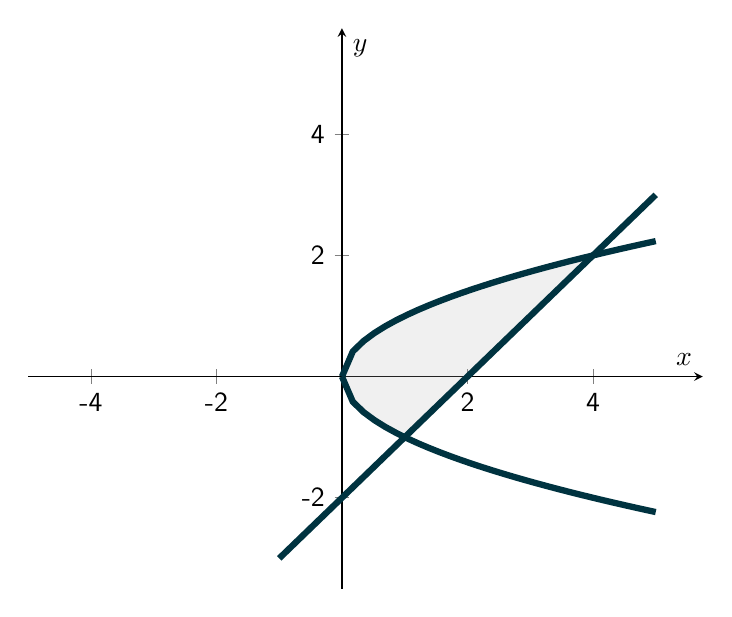
\begin{tikzpicture}[scale=1.25]
            \begin{axis}[
            axis lines = middle, very thick,
            xlabel = {$x$},
            ylabel = {$y$},
            xmin=-5, xmax=5.75,
            ymin=-3.5, ymax=5.75,
            xtick={-4,-2,0,2,4},
            xticklabels={-4,-2,0,2,4},
            ytick={-2,0,2,4},
            yticklabels={-2,0,2,4}        
            ]
            % Curves
            \addplot [name path = A,-,domain = 0:5, line width=0.8mm,DarkBlue,samples = 30] {sqrt(x)} ;
            \addplot [name path = B,-,domain = 0:5, line width=0.8mm,DarkBlue,samples = 30] {-sqrt(x)} ;
            \addplot [name path = C, line width=0.8mm, samples=4, smooth,domain=0:5, DarkBlue] coordinates {(-1,-3)(5,3)};
            % Fill area between paths
            \addplot [black!30, opacity=0.2] fill between [of = A and B, soft clip={domain=0:1}];
            \addplot [black!30, opacity=0.2] fill between [of = A and C, soft clip={domain=1:4}];
            \end{axis}
        \end{tikzpicture}    
    \end{center}   
        
    Thus
    \begin{align}
        \bar y &= \frac{M_x}M = \frac1M \int_{-1}^{2}\int_{y^2}^{y+2} 12y \, dx \, dy
    \end{align} 
    Thus
    \begin{align}
        a &= -1 \\
        b &= 2 \\
        c&= y^2 \\
        d&= y+2 \\
        f(x,y) &= \delta y = 12y
    \end{align}
    }
   \else

   \fi
    
\fi

\ifnum \Version=7
% SHORT SPHERICAL AND CYLINDRICAL EXERCISE
\part Point $P$ has rectangular (Cartesian) coordinates $(x,y,z) = (-6,0,8)$ in $\mathbb R^3$. In cylindrical coordinates, the point is $(r,\theta,z)$, and in spherical coordinates the point is $(\rho, \phi, \theta)$. Where $r=\framebox{\strut\hspace{1cm}}$, $\theta=\framebox{\strut\hspace{2cm}}$, $z=\framebox{\strut\hspace{1cm}}$, $\rho=\framebox{\strut\hspace{2cm}}$, and $\phi=\framebox{\strut\hspace{3cm}}$. 

    \ifnum \Solutions=1 {\color{DarkBlue} \textit{Solutions:} To convert to cylindrical we can use the equation $r^2 = x^2 + y^2$. 
    \begin{align}
        r^2 &= x^2 + y^2 = (-6)^2 + 0^2 = 36 \ \Rightarrow \ r = 6
    \end{align}
    To determine $\theta$ we can use $\tan\theta = y/x$. 
    \begin{align}
        \tan \theta &= \frac{y}{x} = \frac{0}{-6} = 0  \\
        \theta &= \arctan 0 
    \end{align} 
    The point in cylindrical is: 
    \begin{align}
        (r,\theta,z) &= (6,\pi,8) \\
        r &= 6 \\
        \theta &= \pi \\
        z &= 8
    \end{align}
    In spherical, we can start by obtaining $\rho$. 
    \begin{align}
        \rho^2 &= x^2+y^2+z^2\\
        \rho^2 &= (-6)^2 + 0^2 + 8^2 = 36+64 = 100 \\
        \rho &= 10
    \end{align}
    To obtain $\phi$ we can use the equation that relates $x$ to spherical. Using the expression for $x$, and the values that we already have for $x$, $\rho$ and $\theta$:
    \begin{align}
        x &= \rho \sin\phi \cos\theta \\
        -6 &= 10\sin\phi \cos(\pi) \\
        \sin\phi &= \frac{-6}{10 \cos(\pi)}  = \frac{6}{10}\\
        \phi &= \arcsin (6/10)
    \end{align}
    Our coordinates in spherical are
    \begin{align}
        \rho &= 10\\
        \phi &= \arcsin (6/10)\\
        \theta &= \pi
    \end{align}
    Note the following.
    \begin{itemize}
        \item We can, for this exercise, leave un-evaluated trig functions in the answer, because the question didn't specify that you should simplify your answer as much as possible. So it would be ok to leave your answer for $\theta$ as $\arctan 0$ or $\tan^{-1} 0$. 
        \item Our particular textbook uses the convention $(\rho, \phi, \theta)$, not $(\rho, \theta,\phi)$.
    \end{itemize}
    } 
    \else
      
    \fi
    
\fi





\ifnum \Version=8
% SHORT SPHERICAL AND CYLINDRICAL EXERCISE
\part Point $P$ has rectangular (Cartesian) coordinates $(x,y,z) = (4,4,7)$ in $\mathbb R^3$. In cylindrical coordinates, the point is $(r,\theta,z)$, and in spherical coordinates the point is $(\rho, \phi, \theta)$. Where $r=\framebox{\strut\hspace{1cm}}$, $\theta=\framebox{\strut\hspace{2cm}}$, $z=\framebox{\strut\hspace{1cm}}$, $\rho=\framebox{\strut\hspace{2cm}}$, and $\phi=\framebox{\strut\hspace{3cm}}$. 

    \ifnum \Solutions=1 {\color{DarkBlue} \textit{Solutions:} To convert to cylindrical we can use the equation $r^2 = x^2 + y^2$. 
    \begin{align}
        r^2 &= x^2 + y^2 = (4)^2 + 4^2 = 32 \ \Rightarrow \ r = \sqrt{32} = 4\sqrt2
    \end{align}
    It isn't necesssary to simplify to $4\sqrt2$. Then to determine $\theta$ we can use $\tan\theta = y/x$. 
    \begin{align}
        \tan \theta &= \frac{y}{x} = \frac{4}{4} = 1  \\
        \theta &= \arctan \pi/4
    \end{align} 
    The point in cylindrical is: 
    \begin{align}
        (r,\theta,z) &= (4\sqrt2,\pi/4,7) \\
        r &= 4\sqrt2 \\
        \theta &= \pi/4 \\
        z &= 7
    \end{align}
    In spherical, we can start by obtaining $\rho$. 
    \begin{align}
        \rho^2 &= x^2+y^2+z^2\\
        \rho^2 &= (4)^2 + 4^2 + 7^2 = 16+16+49 = 32+49 = 81 \\
        \rho &= 9
    \end{align}
    To obtain $\phi$ we can use the equation that relates $x$ to spherical. Using the expression for $x$, and the values that we already have for $x$, $\rho$ and $\theta$:
    \begin{align}
        x &= \rho \sin\phi \cos\theta \\
        4 &= 9\sin\phi \cos(\pi/4) \\
        \sin\phi &= \frac{4}{9 \cos(\pi/4)}  = \frac{4\sqrt2}{9}\\
        \phi &= \arcsin \left(\frac{4\sqrt2}{9}\right)
    \end{align}
    Note for $\phi$ we can also use:
    \begin{align}
        y &= \rho \sin\phi \sin\theta \\
        4 &= 9\sin\phi \sin(\pi/4) \\
        \sin\phi &= \frac{4}{9 \sin(\pi/4)}  = \frac{4\sqrt2}{9}\\
        \phi &= \arcsin \left(\frac{4\sqrt2}{9}\right)
    \end{align}    
    And we can also use:
    \begin{align}
        z &= \rho \cos\phi  \\
        7 &= 9\cos\phi  \\
        \sin\phi &= \frac{4}{9 \sin(\pi/4)}  = \frac{4\sqrt2}{9}\\
        \phi &= \arccos \left(\frac{7}{9}\right)
    \end{align}      
    Our coordinates in spherical are
    \begin{align}
        \rho &= 9\\
        \phi &= \arcsin \left(\frac{4\sqrt2}{9}\right), \ \textbf{or} \ \phi = \arccos(7/9)\\
        \theta &= \pi/4
    \end{align}
    Note the following.
    \begin{itemize}
        \item We can, for this exercise, leave un-evaluated trig functions in the answer, because the question didn't specify that you should simplify your answer as much as possible. So it would be ok to leave your answer for $\theta$ as $\arctan 1$ or $\tan^{-1} 1$. 
        \item Our particular textbook uses the convention $(\rho, \phi, \theta)$, not $(\rho, \theta,\phi)$.
    \end{itemize}
    } 
    \else
      
    \fi
    
\fi





% 15.6
% CENTROID Y-COORDINATE PARABOLA AND LINE
\ifnum \Version=9
    \part A thin plate with density $\delta=12$ is bounded in the $xy-$plane by $y=3-x^2$ and $y=1-x$. The plate has mass $M$. The $y-$coordinate of the centroid is $\bar y = M_x/M$, where $\displaystyle M_x = \int_A^B \int_C^D f(x,y) \, dy \, dx$,  and $A=\framebox{\strut\hspace{1cm}}$, $B=\framebox{\strut\hspace{1cm}}$, $C=\framebox{\strut\hspace{3cm}}$, $D=\framebox{\strut\hspace{3cm}}$, and $f(x,y) = \framebox{\strut\hspace{3cm}}$. 
    
    \ifnum \Solutions=1 
    {\color{DarkBlue}
    The region is bounded by 
    $$1-x \le y \le 3-x^2$$
    The given curves intersect when 
    \begin{align}
        1-x &= 3-x^2\\
        0 &= x^2-x-2 \\
        &= (x-2)(x+1)
    \end{align}
    The curves intersect at $x=-1,2$. Using $y=1-x$, the intersection points are $(-1,2)$ and $(2,-1)$. The region is shown below. 
    \begin{center}  
        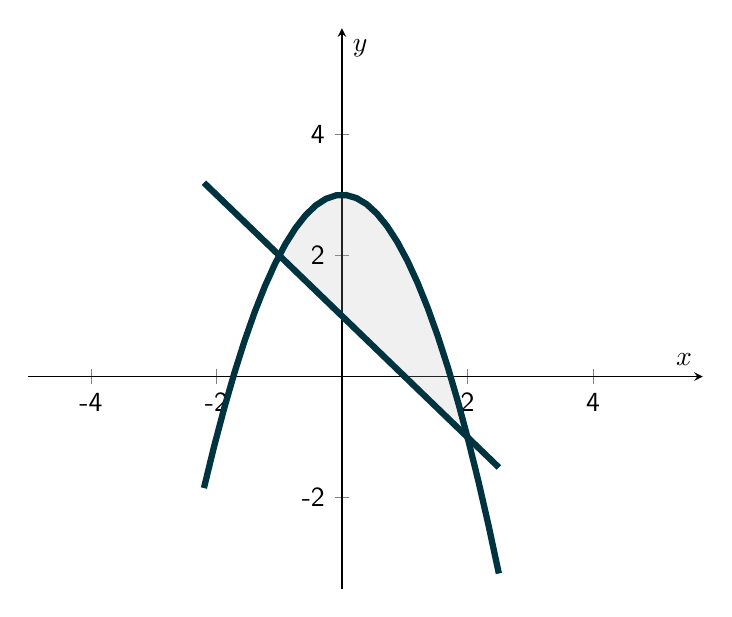
\begin{tikzpicture}[scale=1.25]
            \begin{axis}[
            axis lines = middle, very thick,
            xlabel = {$x$},
            ylabel = {$y$},
            xmin=-5, xmax=5.75,
            ymin=-3.5, ymax=5.75,
            xtick={-4,-2,0,2,4},
            xticklabels={-4,-2,0,2,4},
            ytick={-2,0,2,4},
            yticklabels={-2,0,2,4}        
            ]
            % Curves
            \addplot [name path = A,-,domain = -2.2:2.5, line width=0.8mm,DarkBlue,samples = 30] {3-x^2} ;
            \addplot [name path = C,-,domain = -2.2:2.5, line width=0.8mm,DarkBlue,samples = 4] {1-x} ;
            % Fill area between paths
            \addplot [black!30, opacity=0.2] fill between [of = A and C, soft clip={domain=-1:2}];
            \end{axis}
        \end{tikzpicture}    
    \end{center}   
        
    Thus
    \begin{align}
        \bar y &= \frac{M_x}M = \frac1M \int_{-1}^{2}\int_{1-x}^{3-x^2} 12y \, dy \, dx
    \end{align} 
    Thus
    \begin{align}
        A &= -1 \\
        B &= 2 \\
        C&= 1-x \\
        D&= 3-x^2 \\
        f(x,y) &= \delta y = 12y
    \end{align}
    }
   \else

   \fi
    
\fi
   
    % 13.3 and 13.4
% unit tangent vectors
% arc length
% curvature
% osculating circle
% unit normal

\ifnum \Version=1

\part The unit tangent vector for a curve $\mathbf r(t)$ is $\mathbf T(t) = \langle 0, \cos t, \sin t \rangle$. The unit normal vector is $\mathbf  N = \langle f(t), g(t), g(t) \rangle$, where $f(t) = \framebox{\strut\hspace{2cm}}$, $g(t) = \framebox{\strut\hspace{2cm}}$, $h(t) =\framebox{\strut\hspace{2cm}}$. 

\ifnum \Solutions=1 {\color{DarkBlue} \textit{Answer:} \textit{Solutions:} The normal vector is

\begin{align}
    \mathbf N &= \frac{d\mathbf T/dt}{|d\mathbf T/dt|} 
\end{align}
And
\begin{align}
    \mathbf T'(t) &= \langle 0,-\sin t, \cos t \rangle \\
    |\mathbf T'(t) | &= \sqrt{ 0 +(-\sin t)^2 + (\cos t)^2} =1\\
    \mathbf N &= \frac{d\mathbf T/dt}{|d\mathbf T/dt|} = \langle 0, - \sin(t),  \cos(t) \rangle
\end{align}
} 
\else
\fi        
\fi

\ifnum \Version=2

\part The velocity vector of an object moving on the curve $\mathbf r(t)$ is $\mathbf v(t) = \langle 4\cos (2t), 4\sin (2t) , 3 \rangle$ for $t>0$. The speed of the object for $t>0$ is $s(t) = |\mathbf v | = \framebox{\strut\hspace{1cm}}$. The unit tangent vector for $t>0$ is $\mathbf T = \langle f(t), g(t) , h(t) \rangle$, where $f(t) = \framebox{\strut\hspace{1.5cm}}$, $g(t) = \framebox{\strut\hspace{1.5cm}}$, $h = \framebox{\strut\hspace{1cm}}$. The curvature is $\kappa = \framebox{\strut\hspace{1cm}}$. 

\ifnum \Solutions=1 {\color{DarkBlue} \textit{Answer:} \textit{Solutions:} The speed is the magnitude of the given velocity vector and is
\begin{align}
    s &= |\mathbf v | =  \sqrt{(4\cos2t)^2 + (4\sin2t)^2 + 3^2 } = \sqrt{4^2 (\cos ^2 2 t + \sin^2 2t) + 3^2} = \sqrt{16 + 9} = 5
\end{align}
The unit tangent vector is 
\begin{align}
    \mathbf T &= \frac{\mathbf v}{|\mathbf v|} = \langle \frac{4}{5}\cos(2 t) , \frac 45 \sin (2t), \frac35 \rangle
\end{align}
For curvature we also need
\begin{align}
    \frac{d\mathbf T}{dt } &= \langle -\frac85 \sin 2t, \frac85 \cos 2t,0 \rangle \\
    \left | \frac{d\mathbf T}{dt } \right| &= \sqrt{ \left(-\frac85\sin 2t\right)^2 +   \left(\frac85 \cos 2 t\right)^2 } = \frac85
\end{align}
The curvature is
\begin{align}
    \kappa = \frac{1}{|\mathbf v |}\left| \frac{d\mathbf T}{dt}\right| = \frac{1}{5} \cdot \frac{8}{5} = \frac{8}{25}
\end{align}
} 
\else
\fi        
\fi


\ifnum \Version=3

\part A plane curve $\mathbf r(t)$ has curvature $\kappa = \frac{1}{8}$ at $\mathbf r(t_0) = \langle 15, 2 \rangle$, and the unit normal vector at $t=t_0$ is $\mathbf  N = \mathbf j = \langle 0, 1 \rangle$. The equation of the osculating circle at $t=t_0$ is \framebox{\strut\hspace{3.5cm}}.

\ifnum \Solutions=1 {\color{DarkBlue} \textit{Answer:} \textit{Solutions:} Recall that The circle of curvature, or osculating circle, at a point $P$ on a plane curve where $\kappa \ne 0$ is the circle in the plane of the curve that

\begin{enumerate}
    \item is tangent to the curve at P (has the same tangent line the curve has)
    \item has the same curvature the curve has at P
    \item lies toward the concave or inner side of the curve
\end{enumerate}
The \textbf{radius of curvature} of the curve at P is the radius of the circle of curvature, which is $\frac{1}{\kappa}$. So to obtain the radius, we calculate $\kappa$ and take the reciprocal. The \textbf{center} of the osculating circle of the curve at P lies on the inner side of the curve, and the unit normal points in the direction of the inner side of the planar curve. 

So for this problem we have a circle with radius $1/\kappa = 8$, and whose centre is 8 units away from the point $(15,2)$ in the direction of $\mathbf N$. The circle has equation
$$(x-15)^2 + (y-10)^2 = 8^2$$
} 
\else
  
\fi        
\fi




\ifnum \Version=4

\part The velocity vector for an object moving on the curve $\mathbf r(t)$ is $\mathbf v(t) = \langle t\cos t, t\sin t \rangle$. The speed of the object for $t>0$ is $s(t) = \framebox{\strut\hspace{1cm}}$. The unit tangent vector for $t>0$ is $\mathbf T = \langle f(t), g(t) \rangle$, where $f(t) = \framebox{\strut\hspace{2cm}}$, $g(t) = \framebox{\strut\hspace{2cm}}$. 

\ifnum \Solutions=1 {\color{DarkBlue} \textit{Answer:} \textit{Solutions:} The speed is the magnitude of the velocity vector and is
\begin{align}
    s &= |\mathbf v | = \sqrt{(t\cos t)^2 + (t\sin t)^2 } = \sqrt{t^2 (\cos ^2 t + \sin^2 t)} = |t|
\end{align}
But we are told that $t>0$ so we can use $|t| = t$. The unit tangent vector is 
\begin{align}
    \mathbf T &= \frac{\mathbf v}{|\mathbf v|} = \langle \cos t, \sin t \rangle
\end{align}
} 
\else
\fi        
\fi

\ifnum \Version=5

\part A plane curve $\mathbf r(t)$ has curvature $\kappa = \frac{1}{4}$ at the point $\mathbf r(t_0) = 3\mathbf i + 5\mathbf j$, and the unit normal vector at $t_0$ is $\mathbf  N = \mathbf i = \langle1,0\rangle$. The equation of the osculating circle at $t=t_0$ is \framebox{\strut\hspace{3.5cm}}.

\ifnum \Solutions=1 {\color{DarkBlue} \textit{Answer:} \textit{Solutions:} Recall that The circle of curvature, or osculating circle, at a point $P$ on a plane curve where $\kappa \ne 0$ is the circle in the plane of the curve that

\begin{enumerate}
    \item is tangent to the curve at P (has the same tangent line the curve has)
    \item has the same curvature the curve has at P
    \item lies toward the concave or inner side of the curve
\end{enumerate}
The \textbf{radius of curvature} of the curve at P is the radius of the circle of curvature, which is $\frac{1}{\kappa}$. So to obtain the radius, we calculate $\kappa$ and take the reciprocal. The \textbf{center} of the osculating circle of the curve at P lies on the inner side of the curve, and the unit normal points in the direction of the inner side of the planar curve. 

So for this problem we have a circle with radius $1/\kappa = 4$, and whose centre is 4 units away from the point $(3,5)$ in the direction of $\mathbf N$. The circle has equation
$$(x-7)^2 + (y-5)^2 = 4^2$$
} 
\else
  
\fi        
\fi


\ifnum \Version=6

\part The velocity vector for an object moving on the curve $\mathbf r(t)$ is $\mathbf v(t) = \langle 4t\cos t, 4t\sin t \rangle$ for $t>0$. The speed of the object for $t>0$ is $s(t)  = |\mathbf v | = \framebox{\strut\hspace{1cm}}$. The unit tangent vector for $t>0$ is $\mathbf T = \langle f(t), g(t) \rangle$, where $f(t) = \framebox{\strut\hspace{1.5cm}}$, $g(t) = \framebox{\strut\hspace{1.5cm}}$. The curvature is $\kappa = \framebox{\strut\hspace{1cm}}$. 

\ifnum \Solutions=1 {\color{DarkBlue} \textit{Answer:} \textit{Solutions:} The speed is the magnitude of the given velocity vector and is
\begin{align}
    s &= |\mathbf v | =  \sqrt{(4t\cos t)^2 + (4t\sin t)^2 } = \sqrt{4^2t^2 (\cos ^2 t + \sin^2 t)} = 4|t|
\end{align}
But we are told that $t>0$ so we can assume $|t| = t$. The unit tangent vector is 
\begin{align}
    \mathbf T &= \frac{\mathbf v}{|\mathbf v|} = \langle \cos t, \sin t \rangle
\end{align}
We need
\begin{align}
    \frac{d\mathbf T}{dt } &= \langle -\sin t, \cos t \rangle \\
    \left | \frac{d\mathbf T}{dt } \right| &= \sqrt{ (-\sin t)^2 +   \cos^2 t } = 1
\end{align}
The curvature is
\begin{align}
    \kappa = \frac{1}{|\mathbf v |}\left| \frac{d\mathbf T}{dt}\right| = \frac{1}{4t} 
\end{align}
} 
\else
\fi        
\fi



\ifnum \Version=7

\part The velocity vector of an object moving on the curve $\mathbf r(t)$ is $\mathbf v(t) = \langle 3\cos (2t), 3\sin (2t) \rangle$ for $t>0$. The speed of the object for $t>0$ is $s(t) = |\mathbf v | = \framebox{\strut\hspace{1.5cm}}$. The unit tangent vector for $t>0$ is $\mathbf T = \langle f(t), g(t)  \rangle$, where $f(t) = \framebox{\strut\hspace{2cm}}$, and $g(t) = \framebox{\strut\hspace{2cm}}$.  The curvature for $t>0$ is \framebox{\strut\hspace{1.5cm}}. 

\ifnum \Solutions=1 {\color{DarkBlue} \textit{Answer:} \textit{Solutions:} The speed is the magnitude of the given velocity vector and is
\begin{align}
    s &= |\mathbf v | =  \sqrt{(3\cos t)^2 + (3\sin t)^2  } = \sqrt{3^2 (\cos ^2 t + \sin^2 t) + 3^2} = \sqrt{ 9} = 3
\end{align}
The unit tangent vector is 
\begin{align}
    \mathbf T &= \frac{\mathbf v}{|\mathbf v|} 
    = \langle \frac{3}{3}\cos(2 t) , \frac 33 \sin (2t) \rangle 
    = \langle \cos(2 t) ,  \sin (2t) \rangle
\end{align}
For curvature we also need
\begin{align}
    \frac{d\mathbf T}{dt } &= \langle -2 \sin 2t, 2 \cos 2t\rangle \\
    \left | \frac{d\mathbf T}{dt } \right| &= \sqrt{ \left(-2\sin 2t\right)^2 +   \left(2 \cos 2 t\right)^2 } = 2
\end{align}
The curvature is
\begin{align}
    \kappa = \frac{1}{|\mathbf v |}\left| \frac{d\mathbf T}{dt}\right| = \frac{1}{3} \cdot 2 = \frac{2}{3}
\end{align}
} 
\else
\fi        
\fi


\ifnum \Version=8

\part A plane curve $\mathbf r(t)$ has curvature $\kappa = \frac{1}{4}$ at $\mathbf r(t_0) = \langle 5, 3 \rangle$, and the unit normal vector at $t=t_0$ is $\mathbf  N = \mathbf j = \langle 0, 1 \rangle$. The equation of the osculating circle at $t=t_0$ is \framebox{\strut\hspace{3.5cm}}.

\ifnum \Solutions=1 {\color{DarkBlue} \textit{Answer:} \textit{Solutions:} Recall that The circle of curvature, or osculating circle, at a point $P$ on a plane curve where $\kappa \ne 0$ is the circle in the plane of the curve that

\begin{enumerate}
    \item is tangent to the curve at P (has the same tangent line the curve has)
    \item has the same curvature the curve has at P
    \item lies toward the concave or inner side of the curve
\end{enumerate}
The \textbf{radius of curvature} of the curve at P is the radius of the circle of curvature, which is $\frac{1}{\kappa}$. So to obtain the radius, we calculate $\kappa$ and take the reciprocal. The \textbf{center} of the osculating circle of the curve at P lies on the inner side of the curve, and the unit normal points in the direction of the inner side of the planar curve. 

So for this problem we have a circle with radius $1/\kappa = 4$, and whose centre is 4 units away from the point $(5,3)$ in the direction of $\mathbf N$. The circle has equation
$$(x-5)^2 + (y-7)^2 = 4^2$$
} 
\else
  
\fi        
\fi






\ifnum \Version=9

\part The velocity vector of an object moving on the curve $\mathbf r(t)$ is $\mathbf v(t) = \langle t, 3 \rangle$ for $t>0$. The speed of the object at $t=2$ is $s(2) = |\mathbf v(2) | = \framebox{\strut\hspace{1.75cm}}$. The unit tangent vector at $t=2$ is $\mathbf T(2) = \langle c_1 ,c_2  \rangle$, where $c_1 = \framebox{\strut\hspace{1.75cm}}$, $c_2 = \framebox{\strut\hspace{1.75cm}}$. The curvature is $\framebox{\strut\hspace{1.75cm}}$. 

\ifnum \Solutions=1 {\color{DarkBlue} \textit{Answer:} \textit{Solutions:} The speed is the magnitude of the given velocity vector and is
\begin{align}
    s &= |\mathbf v | =  \sqrt{( t)^2 + (3)^2  } = \sqrt{t^2+9}\\
    s(2) &= \sqrt{2^2+9} = \sqrt{13}
\end{align}
We also need the unit tangent vector at $t=2$. 
\begin{align}
    \mathbf T (t) &= \frac{\mathbf v}{|\mathbf v|} = \frac{t\mathbf i + 3\mathbf j}{\sqrt{t^2+9}} \\
    \mathbf T (2) &= \frac{2\mathbf i + 3\mathbf j}{\sqrt{2^2+9}}  
    = \langle \frac{2}{\sqrt{13}} , \frac {3}{\sqrt{13}}  \rangle \\
    c_1 &= \frac{2}{\sqrt{13}}\\
    c_2 &= \frac{3}{\sqrt{13}}
\end{align}
The curvature is zero because the motion is along a straight line. 
\begin{align}
    \kappa = 0
\end{align}
} 
\else
\fi        
\fi

\ifnum \Version=10

\part A plane curve $\mathbf r(t)$ has curvature $\kappa = \frac{1}{10}$ at $\mathbf r(t_0) = \langle 5, 0 \rangle$, and the unit normal vector at $t=t_0$ is $\mathbf  N = \mathbf j = \langle 0, 1 \rangle$. The equation of the osculating circle at $t=t_0$ is \framebox{\strut\hspace{3.5cm}}.

\ifnum \Solutions=1 {\color{DarkBlue} \textit{Answer:} \textit{Solutions:} Recall that The circle of curvature, or osculating circle, at a point $P$ on a plane curve where $\kappa \ne 0$ is the circle in the plane of the curve that

\begin{enumerate}
    \item is tangent to the curve at P (has the same tangent line the curve has)
    \item has the same curvature the curve has at P
    \item lies toward the concave or inner side of the curve
\end{enumerate}
The \textbf{radius of curvature} of the curve at P is the radius of the circle of curvature, which is $\frac{1}{\kappa}$. So to obtain the radius, we calculate $\kappa$ and take the reciprocal. The \textbf{center} of the osculating circle of the curve at P lies on the inner side of the curve, and the unit normal points in the direction of the inner side of the planar curve. 

So for this problem we have a circle with radius $1/\kappa = 10$, and whose centre is 10 units away from the point $(5,0)$ in the direction of $\mathbf N$. The circle has equation
$$(x-5)^2 + (y-10)^2 = 10^2$$
} 
\else
  
\fi        
\fi
   
\end{parts}

\newpage \question[0.25] \ID
% CHANGE OF VARIABLE (15.8)
% OR APPLICATION (15.6)
% OR TRIPLE CARTESIAN (15.5) 

\ifnum \Version=1
% CENTROID
% BASED ON THOMAS EXERCISES, 15.6 #1
% SUFFICIENT FOR A PRACTICE EXAM
\question[6] A thin plate of density $\delta(x,y) = 12x$ is bounded by the lines $x = 0, y = x$, and the parabola $y = x^2-6$ in the first quadrant. 
\begin{parts} 
    \part Determine the mass of the plate, $M$. Please show your work. 
    \ifnum \Solutions=1 
    {\color{DarkBlue} \textit{Solutions:}
    Curves intersect when $$x = x^2-6 \quad \Rightarrow \quad 0 = x^2 - x - 6 = (x-3)(x+2)$$
    Or $x=3, -2$. We can ignore $x=-2$ because the region is the first quadrant. Curves intersect at the point $(3,3)$, and 
    \begin{align}
        0 \le y \le 3, \quad y \le x \le \sqrt{y+6}
    \end{align}
    The mass is
    \begin{align}
        M &= \int_0^3 \int_y^{\sqrt{y+6}} \delta \, dx \, dy \\
        &= \int_0^3 \int_y^{\sqrt{y+6}} 12x \, dx \, dy \\
        &= \int_0^3  \left. 6x^2 \right|_{x=y}^{x=\sqrt{y+6}} \, dy \\
        &= \int_0^3 6(y + 6 - y^2) \, dy \\
        &= \int_0^3 6y + 36 - 6y^2 \, dy \\
        &= \left. (3y^2 + 36y - 2y^3 ) \right|_0^3 \, dy \\
        &= 27 + 108 - 54 \\
        &= 81
    \end{align}
    }
    \else 
    \vspace{16cm}
    \fi
    \part Use your results from the previous part to set up an integral that can be used to determine the $x-$coordinate of the center of mass of the plate. You do not need to evaluate your integral. 
    \ifnum \Solutions=1 {\color{DarkBlue} \textit{Solutions:} the $x-$coordinate of the center of mass, $\bar x$, is
    \begin{align}
    \bar x &= \frac{M_y}{M} = \frac{1}{81} \int_0^3 \int_y^{\sqrt{y+6}} 12x^2 \, dx \, dy 
    \end{align}
    } 
    \else
      
    \fi
    \end{parts} 
\fi
    





\ifnum \Version=2
% LONGISH CHANGE OF VARIABLE
% VERBATUM FROM SPRING 2022 QUIZ
% hand written solution only
% SUFFICIENT FOR A PRACTICE EXAM
\question[6] Consider the double integral

$$I=\iint_R \frac{x+2y}{2y-x} dA$$

where $R$ is the parallelogram with vertices $(-3,1), (-1,0), (-1,2), (1,1)$. Our goal is to determine the area of the parallelogram using the transform below. 
$$u=x+2y, \qquad v = -x +2y$$ 
Please show your work for the following. 
\begin{parts} 
    \part Use the given transform to calculate the Jacobian of the transform, $J = \partial x(u,v)/\partial y(u,v)$. 
    \ifnum \Solutions=1 
    \else 
    \vspace{8 cm}
    \fi
    \part Use your results from Part (a) and the given transform to transform the double integral. You do not need to evaluate your integral. 
\end{parts} 

\ifnum \Solutions=1 {\color{DarkBlue} \textit{Solutions:} the integral after the transform is $$\displaystyle \frac14 \int_1^5\int_{-1}^3 \frac uv \, du \, dv$$
A screen capture of a hand-written solution from a previous offer of MATH 2551 is below. 
    \begin{figure}[h]
    \centering
    \includegraphics[width=16cm]{202302/Exam3/Images/ImgE3.OR.06.png}
    \end{figure}  
    
    } 
   \else
      
   \fi
    
\fi

\ifnum \Version=3
% CENTROID
% BASED ON THOMAS EXERCISES, 15.6 #1
% SUFFICIENT FOR A PRACTICE EXAM
\question[6] A thin plate with density $\delta(x,y) = 24y$ is bounded by the lines $x = 0, x=2y$, and the parabola $x=y^2$ in the first quadrant. 
\begin{parts} 
    \part Determine the mass of the plate, $M$. Please show your work. 
    
    \ifnum \Solutions=1 
    {\color{DarkBlue} \textit{Solutions:}
    Curves intersect when $$2y = y^2 \quad \Rightarrow \quad 0 = y^2-2y = y(y-2)$$
    Or $y=0,2$. Curves intersect at the points $(0,0)$, $(4,2)$. 
    The mass is
    \begin{align}
        M = \int_0^4 \int_{x/2}^{\sqrt{x}} \delta \, dy \, dx 
        &= \int_0^4 \int_{x/2}^{\sqrt{x}} 24y \, dy \, dx \\
        &= \int_0^4  \left. 12y^2 \right|_{y=x/2}^{y=\sqrt{x}} \, dx \\
        &= 12 \int_0^4 (x-\frac{x^2}{4}) \, dx \\
        &= 12 \left. (\frac{x^2}{2} - \frac{x^3}{12} ) \right|_0^4 \, dy \\
        &= 12 (\frac{16}{2} - \frac{64}{12}) \\
        &= 96 - 64\\
        &= 32
    \end{align}
    \textbf{An Alternate Solution}\\
    Another way to approach this problem is to use the integration order $dx\,dy$. In this case the double integral becomes
    \begin{align}
        M = \int_0^2 \int_{y^2}^{2y} \delta \, dx \, dy
        &= \int_0^2 \int_{y^2}^{2y} 24y \, dx \, dy \\
        &= 24\int_0^2  \left. yx \right|_{x=y^2}^{x=2y} \, dy \\
        &= 24 \int_0^2 (2y^2 - y^3) \, dy \\
        &= 24 \left. (\frac{2y^3}{3} - \frac{y^4}{4} ) \right|_0^2 \, dy \\
        &= 24 (\frac{16}{3} - \frac{16}{4}) \\
        &= \frac{24\cdot16}{3} - 24\cdot 4 \\
        &= 8\cdot16 - 96 \\
        &= 128 - 96 \\
        &= 32
    \end{align}    
    }
    \else 
    \vspace{14cm}
    \fi
    \part Use your results from the previous part to set up an integral that can be used to determine the $x-$coordinate of the center of mass of the plate. You do not need to evaluate your integral. 
    \ifnum \Solutions=1 {\color{DarkBlue} \textit{Solutions:} the $x-$coordinate of the center of mass, $\bar x$, is
    \begin{align}
    \bar x &= \frac{M_y}{M} = \frac{1}{32} \int_0^4 \int_{x/2}^{\sqrt{x}} 24xy \, dy \, dx
    \end{align}
    \textbf{An Alternate Solution}\\    
    It is also ok to use the integration order $dx\,dy$. In this case the double integral becomes
    \begin{align}
    \bar x &= \frac{M_y}{M} = \frac{1}{32} \int_0^2 \int_{y^2}^{2y} 24xy \, dx \, dy 
    \end{align}
    } 
    \else
      
    \fi
    \end{parts} 
\fi

\ifnum \Version=4
% VERSION B
% LONG CHANGE OF VARIABLE
% BASED ON AN EXAMPLE FROM THOMAS
% SECTION 15.8 FROM THOMAS
\question[6] Consider the double integral

$$I= 9 \iint_R (y-2x)^2 \sqrt{x+y} \, dA$$

where $R$ is the region in the first quadrant bounded by the lines $x=0$, $y=0$, and $y=1-x$. Our goal is to determine the area of $R$ using the transform below. 
$$u=x+y, \qquad v = y-2x$$ 
Please show your work for the following. 
\begin{parts} 
    \part Use the given transform to calculate the Jacobian of the transform, $J = \partial x(u,v)/\partial y(u,v)$. 
    \ifnum \Solutions=1 {\color{DarkBlue} \textit{Solutions:} Solving for $x$ and $y$ using an augmented matrix,
    \begin{align}
        \begin{pmatrix} 1 & 1 & u \\-2 & 1 & v\end{pmatrix} 
        \sim \begin{pmatrix} 1 & 1 & u \\0 & 3 & 2u+v\end{pmatrix} 
        \sim \begin{pmatrix} 1 & 0 & u/3 - v/3 \\0 & 1 & 2u/3+v/3 \end{pmatrix} 
    \end{align}
    Thus
    \begin{align}
        x &= \frac13(u-v), \ y = \frac13(2u+v) \\
        J(u,v) & = \begin{vmatrix} \DXDU & \DXDV \\[8pt] \DYDU & \DYDV \end{vmatrix} = \begin{vmatrix} 1/3 & -1/3 \\ 2/3 & 1/3 \end{vmatrix} = 1/9 + 2/9 = 1/3
    \end{align}
    }
    \else 
    \vspace{8 cm}
    \fi
    \part Use the given transform and your results from Part (a) to convert the double integral into a double integral over a region in the $uv-$plane. You do not need to evaluate your integral. 
    \ifnum \Solutions=1 {\color{DarkBlue} \textit{Solutions:} Converting each of the boundaries in the $xy-$plane into the $uv-$plane we obtain
        \begin{align}
            x+y &= 1 \quad \Rightarrow \quad \frac13(u-v) + \frac13(2u+v) = 1 &&\Rightarrow \quad u = 1\\
            x&=0 \quad \Rightarrow \quad \frac13(u-v) = 0 &&\Rightarrow \quad v = u\\
            y&= 0 \quad \Rightarrow \quad \frac13(2u+v) = 0 &&\Rightarrow \quad v = -2u
        \end{align}
        The region is described by either of the following relations:
        \begin{align}
            S_1: & \quad 0 \le u \le 1, \quad -2u \le v \le u \\
            S_2: & \quad -2 \le v \le 0, \quad -v/2 \le u \le 1, \ \text{and } 0 \le v \le 1, \quad v \le u \le 1
        \end{align}
        The first set of inequalities requires only a single double integral, but it is ok to set up two double integrals. If using $S_1$, we use $dv\,du$ and obtain
        \begin{align}
            I= 9 \iint_R (y-2x)^2 \sqrt{x+y} \, dA = 9 \int_0^1 \int_{-2u}^u v^2u^{1/2} \frac13 \,dv\,du
        \end{align}
        If using $S_2$, we use $du\,dv$ and obtain
        \begin{align}
            I= 9 \iint_R (y-2x)^2 \sqrt{x+y} \, dA 
            = 9 \int_{-2}^0 \int_{-v/2}^1 v^2u^{1/2} \frac13 \,du\,dv
            + 9 \int_{0}^1 \int_{v}^1 v^2u^{1/2} \frac13 \,du\,dv
        \end{align}        
        } 
       \else
          
       \fi
    \end{parts} 

    \fi



\ifnum \Version=5
    % USE FOR VERSION B
    % LONG CYLINDRICAL WITH APPLICATION TO MASS WITH VARYING DENSITY
    % FROM 15.8
    \question[6] An object $D$ lying in the first octant is bounded below by the $xy-$plane, above by the plane $z=3+4y$, and by the cylinder $x^2+y^2 = 4$. The density of the object at any point in $D$ is equal to the distance from the point to the $z$-axis.  Please show your work for the following.
    
    \begin{parts} 
    \part Use cylindrical coordinates to calculate the total of mass of the object, $M$. Please show your work. 
    
    \ifnum \Solutions=1 {\color{DarkBlue} The object is only in the first octant so $$0 \le \theta \le \pi/2$$ Using $\delta = \sqrt{x^2+y^2} = r$, the $z-$coordinate of the center of mass is computed using 
    \begin{align}
        M &= \iiint_D  \delta \, dV \\
        &= \int_0^{\pi/2} \int_0^2 \int_0^{3+4r\sin\theta}  \delta(r,\theta) \, r\, dz\,dr\,d\theta\\
        &= \int_0^{\pi/2} \int_0^2 \int_0^{3+4r\sin\theta}   r^2 \, dz\,dr\,d\theta\\
        &= \int_0^{\pi/2} \int_0^2    r^2 \, (3+4r\sin\theta) \,dr\,d\theta \\
        &= \int_0^{\pi/2} \int_0^2     \, (3r^2+4r^3\sin\theta) \,dr\,d\theta \\
        &= \int_0^{\pi/2}  \left. \, (r^3+r^4\sin\theta) \right|_{r=0}^{r=2} d\theta \\
        &= \int_0^{\pi/2}  (8 + 16\sin\theta) d\theta \\
        &=  \left. (8\theta - 16\cos\theta) \right|_0^{\pi/2} \\
        &=  (4\pi - 0) - (0 - 16) \\
        &= 4\pi + 16
    \end{align}
    
    } 
    \else
        \vspace{14cm}
    \fi
    
    \part Use your results from the previous part to set up a triple integral in cylindrical coordinates that can be used to determine the $z-$coordinate of the center of mass of the object. You do not need to evaluate your integral. 

    \ifnum \Solutions=1 {\color{DarkBlue} \textit{Solutions:} the $z-$coordinate of the center of mass, $\bar x$, is
    \begin{align}
    \bar z &= \frac{M_{xy}}{M} = \frac{1}{16\pi+16} \int_0^{\pi/2} \int_0^2 \int_0^{3+4r\sin\theta}  z \, \delta(r,\theta) \, r\, dz\,dr\,d\theta
    \end{align}
    } 
    \else
      
    \fi
    \end{parts} 
\fi


% TRANSFORM: SOLVE FOR X & Y, BOUNDARIES, EVALUATE, TRIANGLES
% VERSION A
\ifnum \Version=6
    \question[6] Consider the transform $u=x+y$ and $v=4x+5y$, and the integral $\displaystyle I = \iint_{R}  \,dxdy$. Region $R$ is the triangle in the $xy$-plane bounded by $x+y=0$, $4x+5y=0$, $6x+7y=4$. The transform maps $R$ to region $G$ in the $uv-$plane.  Please show your work for the following.

    \begin{enumerate}
        \item[a)] Solve the system, $u=x+y$ and $v=4x+5y$, for $x$ and $y$ in terms of $u$ and $v$.
            \ifnum \Solutions=1 {\color{DarkBlue} \\[12pt] 
            \textbf{Solutions:}
            We can use the expressions for $u$ and $v$ as an augmented matrix and row reduce. 
            \begin{align}
                \begin{pmatrix} 1 & 1 & u \\ 4 & 5 & v\end{pmatrix} 
                \sim \begin{pmatrix} 1 & 1 & u \\0 & 1 & v - 4u \end{pmatrix} 
                \sim \begin{pmatrix} 1 & 0 & 5u - v \\ 0 & 1 & v - 4u \end{pmatrix} 
            \end{align}
            Thus $x = 5u - v$, and $y = v - 4u$. 
            } 
            \else 
            \vspace{5cm}
            \fi
        \item[b)] Transform the boundaries of $R$ to the $uv-$plane. In other words, determine the boundaries of $G$ in terms of $u$ and $v$. 
            \ifnum \Solutions=1 {\color{DarkBlue} \\[12pt] 
            \textbf{Solutions:} the three lines are transformed below. 
            \begin{itemize}
                \item The line $x+y=0$ becomes $u=0$. 
                \item The line $4x+5y=0$ becomes $v=0$. 
                \item The line $6x+7y=4$ is: 
                \begin{align}
                    6x+7y &=4 \\
                    6\cdot(5u-v) + 7\cdot(v-4u) &= 4\\
                    30u -28u -6v+7v &=4 \\
                    v &= 4 -2u
                \end{align}
            \end{itemize}
            } 
        \else 
        \vspace{5cm}
        \fi        
            
        \item[c)] Use the given transformation and your results from parts (a) and (b) to set up a double integral that in the $uv-$plane that is equal to $I$. Do not evaluate the integral. You also do not need to calculate the Jacobian and may use that the Jacobian of the transform is $J(u,v) = 1$.
            \ifnum \Solutions=1 {\color{DarkBlue} \\[12pt] 
            \textbf{Solutions:}
            \begin{align}
                \iint_{R} \,dx\,dy
                &= \iint_{G}  \left| J(u,v) \right| \,dv\,du 
                = \int_0^2\int_{0}^{4-2u}  \left| 1 \right| \,dv\,du 
                = \int_0^2\int_{0}^{4-2u} \,dv\,du
            \end{align}
            Note the following.
            \begin{itemize}
                \item We did not need to compute the Jacobian but it is computed as follows. 
                $$J 
                = \begin{vmatrix} x_u & x_v \\ y_u & y_v \end{vmatrix} 
                = \begin{vmatrix} 5 & -1 \\ -4 & 1\end{vmatrix} 
                = 5 - 4
                = 1$$
                \item             We did not need to evaluate the integral but if we did:
            \begin{align}
                I = \int_0^2\int_{0}^{4-2u}  \left| 1 \right| \,dv\,du
                = 1 \int_0^2 (4-2u) \,du
                =  \left. 4u - u^2 \right|_0^2 
                = 4
            \end{align}
            \item It is also ok to use the other integration order: $I = \int_0^4\int_0^{2-v/2} \, du \, dv$.
            \end{itemize}
            } 
            \else 
            \fi        
    \end{enumerate}
 
\fi 



% TRANSFORM: SOLVE FOR X & Y, BOUNDARIES, EVALUATE, PARALLELOGRAM
% VERSION A
\ifnum \Version=7
    \question[6] Consider the integral $\displaystyle I = 2\iint_{R} x-4y \,dx\,dy$, where $R$ is the parallelogram in the $xy$-plane bounded by $x-4y=2$, $x-4y=1$, $3y-x=3$, $3y-x=6$. Suppose the transform $u=x-4y$ and $v=3y-x$, maps region $R$ to region $G$ in the $uv-$plane.  Please show your work for the following.

    \begin{enumerate}
        \item[a)] Solve the system, $u=x-4y$ and $v=3y-x$, for $x$ and $y$ in terms of $u$ and $v$.
            \ifnum \Solutions=1 {\color{DarkBlue} \\[12pt] 
            \textbf{Solutions:}
            We can use the expressions for $u$ and $v$ as an augmented matrix and row reduce. 
            \begin{align}
                \begin{pmatrix} 1 & -4 & u \\ -1 & 3 & v\end{pmatrix} 
                \sim \begin{pmatrix} 1 & -4 & u \\0 & -1 & v + u\end{pmatrix} 
                \sim \begin{pmatrix} 1 & 0 & -3u-4v\\0 & 1 & -u-v\end{pmatrix} 
            \end{align}
            Thus
            \begin{align}
                x &=  -3u-4v\\
                y &= -u-v
            \end{align}

            } 
            \else 
            \vspace{5cm}
            \fi
        \item[b)] Transform the boundaries of $R$ to the $uv-$plane. In other words, determine the boundaries of $G$ in terms of $u$ and $v$. 
            \ifnum \Solutions=1 {\color{DarkBlue} \\[12pt] 
            \textbf{Solutions:} the four lines are transformed below. 
            \begin{itemize}
                \item The line $x-4y=2$ becomes $u=2$. 
                \item The line $x-4y=1$ becomes $u=1$. 
                \item The line $3y-x=3$ becomes $v=3$. 
                \item The line $3y-x=6$ becomes $v=6$. 
            \end{itemize}
            } 
        \else 
        \vspace{5cm}
        \fi        
            
        \item[c)] Use the given transformation and your results from parts (a) and (b) to set up a double integral that in the $uv-$plane that is equal to $I$. Do not evaluate the integral. You also do not need to calculate the Jacobian and may use that the Jacobian of the transform is  $J(u,v) = -1$. 
            \ifnum \Solutions=1 {\color{DarkBlue} \\[12pt] 
            \textbf{Solutions:}
            \begin{align}
                \iint_{R} 2x-8y \,dx\,dy
                = \iint_{G} 2u \left| J(u,v) \right| \,du\,dv
                = \int_3^6\int_{1}^2 2u \left| -1 \right| \,du\,dv
                = \int_3^6\int_{1}^2 2u \,du\,dv
            \end{align}
            Note the following.
            \begin{itemize}
                \item We did not need to evaluate the integral, but if we did: 
                \begin{align}
                \iint_{R} 2x-8y \,dx\,dy
                &= \iint_{G} 2u \left| J(u,v) \right| \,du\,dv\\
                &= \int_3^6\int_{1}^2 2u \left| -1 \right| \,du\,dv\\
                &= \int_3^6\left. u^2 \right|_{1}^2 \,dv\\
                &= \int_3^6 3 \,dv\\
                &= 3 \cdot(6 -3) \\
                &= 9
            \end{align}
            \end{itemize}
            } 
            \else 
            \fi        
    \end{enumerate}
 
\fi 




% TRANSFORM: SOLVE FOR X & Y, BOUNDARIES, EVALUATE
% VERSION B
\ifnum \Version=8
    \question[6] Consider the transform $u=x-y$ and $v=4y-2x$, and the integral $\displaystyle I = \iint_{R} \,dxdy$, where $R$ denotes the triangle in the $xy$-plane bounded by $x-y=2$, $4y-2x=0$, $3y=2x$. The transform maps region $R$ to region $G$ in the $uv-$plane.  Please show your work for the following.

    \begin{enumerate}
        \item[a)] Solve the system, $u=x-y$ and $v=4y-2x$, for $x$ and $y$ in terms of $u$ and $v$.
            \ifnum \Solutions=1 {\color{DarkBlue} \\[12pt] 
            \textbf{Solutions:}
            We can use the expressions for $u$ and $v$ as an augmented matrix and row reduce. 
            \begin{align}
                \begin{pmatrix} 1 & -1 & u \\ -2 & 4 & v\end{pmatrix} 
                \sim \begin{pmatrix} 1 & -1 & u \\0 & 2 & v + 2u\end{pmatrix} 
                \sim \begin{pmatrix} 1 & -1 & u\\0 & 1 & u+v/2\end{pmatrix} 
                \sim \begin{pmatrix} 1 & 0 & 2u+v/2\\0 & 1 & u+v/2\end{pmatrix} 
            \end{align}
            Thus $x = 2u+v/2$, and $y = u + \frac{v}{2}$. 
            } 
            \else 
            \vspace{5cm}
            \fi
        \item[b)] Transform the boundaries of $R$ to the $uv-$plane. In other words, determine the boundaries of $G$ in terms of $u$ and $v$. 
            \ifnum \Solutions=1 {\color{DarkBlue} \\[12pt] 
            \textbf{Solutions:} the three lines are transformed below. 
            \begin{itemize}
                \item The line $x-y=2$ becomes $u=2$. 
                \item The line $4x-2y=0$ becomes $v=0$. 
                \item The line $3y=2x$ is: 
                \begin{align}
                    3\cdot \left(u+\frac{v}{2}\right) &= 2\cdot \left( 2u+v/2 \right) \\
                    3u + 3v/2 &= 4u + v \\
                    v/2 &= u \\
                    v &= 2u 
                \end{align}
            \end{itemize}
            } 
        \else 
        \vspace{5cm}
        \fi        
            
        \item[c)] Use the given transformation and your results from parts (a) and (b) to set up a double integral that in the $uv-$plane that is equal to $I$. Do not evaluate the integral. You also do not need to calculate the Jacobian and may use that the Jacobian of the transform is  $J(u,v) = \frac12$. 
            \ifnum \Solutions=1 {\color{DarkBlue} \\[12pt] 
            \textbf{Solutions:} the region is
            $$G = \{ (u,v) \in \mathbb R^2 \, | \, 0\le u \le 2, \ 0 \le v \le 2u\}$$
            or we can use
            $$G = \{ (u,v) \in \mathbb R^2 \, | \, 0\le v \le 4, \ v/2 \le u \le 4\}$$ 
            We can write the double integral as:
            \begin{align}
                \iint_{R} \,dx\,dy
                = \iint_{G}  \left| J(u,v) \right| \,dv\,du 
                = \int_0^2\int_{0}^{2u}  \left| \frac12 \right| \,dv\,du
                = \frac12 \int_0^2\int_{0}^{2u} \,dv\,du
            \end{align}
            Note the following.
            \begin{itemize}
                \item We did not need to compute the Jacobian but it is computed as follows. 
                $$J = \begin{vmatrix} x_u & x_v \\ y_u & y_v \end{vmatrix} = \begin{vmatrix} 2 & 1/2 \\ 1 & 1/2\end{vmatrix} = 1 - 1/2 = \frac12$$
                \item We didn't need to evaluate the integral but if we did: 
                \begin{align}
                \iint_{R} \,dx\,dy
                    &= \iint_{G}  \left| J(u,v) \right| \,dv\,du\\
                    &= \int_0^2\int_{0}^{2u}  \left| \frac12 \right| \,dv\,du\\
                    &= \frac12 \int_0^2\left.  v \right|_{v=0}^{v=2u} \,du\\
                    &= \frac12 \int_0^2 2u \,du\\
                    &=  \int_0^2 u \,du\\
                    &= \frac12 \left. u^2\right|_0^2 \\
                    &= 2
            \end{align}                
            \end{itemize}
            } 
            \else 
            \fi        
    \end{enumerate}
 
\fi 









% TRANSFORM: SOLVE FOR X & Y, BOUNDARIES, EVALUATE
% VERSION D 
\ifnum \Version=9
    \question[6] Consider the transform $u=x+y$ and $v=3x+4y$, and the integral $\displaystyle I = \iint_{R} x+y \,dxdy$, where $R$ denotes the triangle in the $xy$-plane bounded by $x+y=0$, $3x+4y=2$, and $2x+3y=0$. The transform maps region $R$ to region $G$ in the $uv-$plane. Please show your work for the following.

    \begin{enumerate}
        \item[a)] Solve the system, $u=x+y$ and $v=3x+4y$, for $x$ and $y$ in terms of $u$ and $v$.
            \ifnum \Solutions=1 {\color{DarkBlue} \\[12pt] 
            \textbf{Solutions:}
            We can use the expressions for $u$ and $v$ as an augmented matrix and row reduce. 
            \begin{align}
                \begin{pmatrix} 1 & 1 & u \\ 3 & 4 & v\end{pmatrix} 
                \sim \begin{pmatrix} 1 & 1 & u \\0 & 1 & v - 3u \end{pmatrix} 
                \sim \begin{pmatrix} 1 & 0 & 4u - v \\ 0 & 1 & v - 3u \end{pmatrix} 
            \end{align}
            Thus $x = 4u - v$, and $y = v - 3u$. 
            } 
            \else 
            \vspace{5cm}
            \fi
        \item[b)] Transform the boundaries of $R$ to the $uv-$plane. In other words, determine the boundaries of $G$ in terms of $u$ and $v$. 
            \ifnum \Solutions=1 {\color{DarkBlue} \\[12pt] 
            \textbf{Solutions:} the three lines are transformed below. 
            \begin{itemize}
                \item The line $x+y=0$ becomes $u=0$. 
                \item The line $3x+4y=2$ becomes $v=2$. 
                \item The line $2x+3y$ is: 
                \begin{align}
                    2x+3y &=0 \\
                    2\cdot(4u-v) + 3\cdot(v-3u) &= 0\\
                    8u -9u  - 2v+3v &=0 \\
                    v &= u
                \end{align}
            \end{itemize}
            } 
        \else 
        \vspace{5cm}
        \fi        
            
        \item[c)] Use the given transformation and your results from parts (a) and (b) to set up a double integral that in the $uv-$plane that is equal to $I$. Do not evaluate the integral. You also do not need to calculate the Jacobian and may use that the Jacobian of the transform is $J(u,v) = 1$. 
            \ifnum \Solutions=1 {\color{DarkBlue} \\[12pt] 
            \textbf{Solutions:}
            \begin{align}
                \iint_{R} x+y \,dx\,dy
                &= \iint_{G} u \left| J(u,v) \right| \,dv\,du\\
                &= \int_0^2\int_{u}^{2} u \left| 1 \right| \,dv\,du\\
                &= \int_0^2\int_{u}^{2} u  \,dv\,du
            \end{align}
            Note the following.
            \begin{itemize}
                \item We could also instead use
                \begin{align}
                    \iint_{R} x+y \,dx\,dy &= \int_0^2\int_{0}^{v} u  \,du\,dv
                \end{align}
                \item We did not need to compute the Jacobian but it is computed as follows. 
                $$J 
                = \begin{vmatrix} x_u & x_v \\ y_u & y_v \end{vmatrix} 
                = \begin{vmatrix} 4 & -1 \\ -3 & 1\end{vmatrix} 
                = 4 - (-1)(-3)
                = 1$$
                \item It wasn't necessary to compute the integral but: 
                \begin{align}
                    \iint_{R} x+y \,dx\,dy
                    &= \iint_{G} u \left| J(u,v) \right| \,dv\,du\\
                    &= \int_0^2\int_{u}^{2} u \left| 1 \right| \,dv\,du\\
                    &= \int_0^2 2u - u^2 \,du\\
                    &= \left. \left( u^2 - \frac{u^3}{3} \right)\right|_0^2 \\
                    &= 4 - 8/3\\
                    &= 4/3
                \end{align}                
            \end{itemize}
            } 
            \else 
            \fi        
    \end{enumerate}
 
\fi 



\newpage \question[0.25] \ID
% SPHERICAL OR CYLINDRICAL (14.7)


\ifnum \Version=1
% READY TO BE USED FOR PRACTICE EXAM
% SPHERICAL INTEGRATION
% VERBATUM FROM SPRING 2022 QUIZ
% OK FOR A PRACTICE EXAM
% hand written solution only
\question[6] Evaluate the triple integral $I=\displaystyle \iiint_D \frac{16\, x}{\sqrt2}  \, dV$, where $D$ is the region in the first octant bounded by $x^2+y^2+z^2=1$ and the planes $y=0$ and $x=y$. Please show your work. Hint: you may need to use the identity $2\sin ^2x = 1 - \cos(2x)$. 

\ifnum \Solutions=1 {\color{DarkBlue} \textit{Solutions:} below is a screen capture of a hand-written solution from a previous offer of MATH 2551. 
    \begin{figure}[h]
    \centering
    \includegraphics[width=16cm]{202302/Exam3/Images/ImgE3.OR.05.png}
    \end{figure}  
    
    } 
   \else
      
   \fi
    
\fi

\ifnum \Version=2
% OK FOR A PRACTICE EXAM
% NOT SO SHORT CYLINDRICAL EXERCISE
% VERBATUM FROM SPRING 2022 QUIZ
% hand written solution only
\question[6] Use cylindrical coordinates to determine the volume of the region bounded above by $z = 4-3x^2-3y^2$ and bounded below by $z = \sqrt{x^2+y^2}$. Please show your work. 

\ifnum \Solutions=1 {\color{DarkBlue} \textit{Solutions:} below is a screen capture of a hand-written solution from a previous offer of MATH 2551. 
    \begin{figure}[h]
    \centering
    \includegraphics[width=11cm]{202302/Exam3/Images/ImgE3.OR1C.png}
    \end{figure}  
    
    There are other ways to set up this particular integral, but the above is sufficient. 

    } 
   \else
      
   \fi
    
\fi






\ifnum \Version=3
% USE FOR VERSION A
% LONG SPHERICAL WITH APPLICATION TO MASS WITH VARYING DENSITY
% FROM 15.8
\question[6] An object $D$ lying in the first octant is bounded by the planes $x=0, y=0, z=0$, and the sphere $x^2+y^2 + z^2 = 4$. The density of the object at any point in $D$ is equal to the distance from the point to the origin. 

\begin{parts}
    \part Use spherical coordinates to calculate the mass of the object, $M$. Please show your work. 
    
    \ifnum \Solutions=1 {\color{DarkBlue} Using $\delta = \sqrt{x^2+y^2+z^2} = \rho$, the mass is computed using 
    \begin{align}
        M &= \int_0^{\pi/2} \int_0^{\pi/2} \int_0^2 \delta \, \rho^2\sin\phi \, d\rho\,d\phi\,d\theta \\
        &= \int_0^{\pi/2} \int_0^{\pi/2} \int_0^2 \rho^3\sin\phi \, d\rho\,d\phi\,d\theta \\
        &= \int_0^{\pi/2} \int_0^{\pi/2} \left. \frac14 \rho^4\sin\phi \right|_0^2 \, d\phi\,d\theta \\
        &= 4 \int_0^{\pi/2} \int_0^{\pi/2} \sin\phi \, d\phi\,d\theta \\
        &= 4 \int_0^{\pi/2} \left. -\cos\phi \right|_0^{\pi/2} \, d\theta \\
        &= 4 \int_0^{\pi/2}  \, d\theta \\
        &= 2\pi
    \end{align}
    
    } 
   \else
      \vspace{14cm}
   \fi    

   \part Use your results from the previous part to set up an integral in spherical coordinates that can be used to determine the $x-$coordinate of the center of mass of the object. You do not need to evaluate your integral. 
    \ifnum \Solutions=1 {\color{DarkBlue} In spherical coordinates, $$x = \rho \sin\phi \cos\theta$$and the $x-$coordinate of the center of mass, $\bar x$, is
    \begin{align}
    \bar x &= \frac{M_{yz}}{M} \\ 
    &= \frac{1}{M} \int_0^{\pi/2} \int_0^{\pi/2} \int_0^2 (\rho \sin\phi \cos\theta) \, \delta \, \rho^2\sin\phi \, d\rho\,d\phi\,d\theta \\
    &= \frac{1}{M} \int_0^{\pi/2} \int_0^{\pi/2} \int_0^2 \rho^4\sin^2\phi \cos\theta \, d\rho\,d\phi\,d\theta 
    \end{align}
    } 
    \else
      
    \fi
    \end{parts} 
 
\fi








\ifnum \Version=4
% USE FOR VERSION B
% LONG CYLINDRICAL WITH APPLICATION TO MASS WITH VARYING DENSITY
% FROM 15.8
\question[6] An object $D$ lying in the first octant is bounded by the planes $x=0, y=0, z=0$, $z=3+4x$ and the cylinder $x^2+y^2 = 4$. The density of the object at a point in $D$ is equal to the distance from the point to the $z$-axis. 

    \begin{parts} 
    \part Use cylindrical coordinates to calculate the total of mass of the object, $M$. Please show your work. 


    \ifnum \Solutions=1 {\color{DarkBlue} \textit{Solutions:} using $\delta = \sqrt{x^2+y^2} = r$, the $z-$coordinate of the center of mass is computed using 
    \begin{align}
        M &= \iiint_D  \delta \, dV \\
        &= \int_0^{\pi/2} \int_0^2 \int_0^{3+4r\cos\theta}  \delta(r,\theta) \, r\, dz\,dr\,d\theta\\
        &= \int_0^{\pi/2} \int_0^2 \int_0^{3+4r\cos\theta}   r^2 \, dz\,dr\,d\theta\\
        &= \int_0^{\pi/2} \int_0^2 \int_0^{3+4r\cos\theta}   r^2 \, dz\,dr\,d\theta \\ 
        &= \int_0^{\pi/2} \int_0^2    r^2 \, (3+4r\cos\theta) \,dr\,d\theta \\
        &= \int_0^{\pi/2} \int_0^2     \, (3r^2+4r^3\cos\theta) \,dr\,d\theta \\
        &= \int_0^{\pi/2}  \left. \, (r^3+r^4\cos\theta) \right|_0^2 \, d\theta \\
        &= \int_0^{\pi/2}  (8+16\cos\theta) d\theta \\
        &=  \left. (8\theta+16\sin\theta) \right|_0^{\pi/2} \\
        &= 4\pi + 16  
    \end{align}
    
    } 
   \else
      \vspace{14cm}      
   \fi
    \part Use your results from the previous part to set up a triple integral that can be used to determine the $z-$coordinate of the center of mass of the object. You do not need to evaluate your integral. 

    \ifnum \Solutions=1 {\color{DarkBlue} \textit{Solutions:} the $z-$coordinate of the center of mass, $\bar x$, is
    \begin{align}
    \bar z &= \frac{M_{xy}}{M} \\
    &= \frac{1}{16 +4\pi} \int_0^{\pi/2} \int_0^2 \int_0^{3+4r\cos\theta}  z \, \delta(r,\theta) \, r\, dz\,dr\,d\theta
    \end{align}
    } 
    \else
      
    \fi
    \end{parts} 
    
\fi


\ifnum \Version=5
% USE FOR VERSION C
% LONG SPHERICAL WITH APPLICATION TO MASS WITH VARYING DENSITY
% FROM 15.8
\question[6] An object $D$ lies above the $xy-$plane and below the upper half of the sphere $x^2+y^2 + z^2 = 4$. The density of the object at any point in $D$ is equal to the distance from the point to the origin. 

\begin{parts}
    \part Use spherical coordinates to calculate the mass of the object, $M$. Please show your work. 
    
    \ifnum \Solutions=1 {\color{DarkBlue} Using $\delta = \sqrt{x^2+y^2+z^2} = \rho$, the mass is computed using 
    \begin{align}
        M &= \int_0^{2\pi} \int_0^{\pi/2} \int_0^2 \delta \, \rho^2\sin\phi \, d\rho\,d\phi\,d\theta \\
        &= \int_0^{2\pi} \int_0^{\pi/2} \int_0^2 \rho^3\sin\phi \, d\rho\,d\phi\,d\theta \\
        &= \int_0^{2\pi} \int_0^{\pi/2} \left. \frac14 \rho^4\sin\phi \right|_0^2 \, d\phi\,d\theta \\
        &= 4 \int_0^{2\pi} \int_0^{\pi/2} \sin\phi \, d\phi\,d\theta \\
        &= 4 \int_0^{2\pi} \left. -\cos\phi \right|_0^{\pi/2} \, d\theta \\
        &= 4 \int_0^{2\pi}  \, d\theta \\
        &= 8\pi
    \end{align}
    
    } 
   \else
      \vspace{14cm}
   \fi    

   \part Use your results from the previous part to set up an integral in spherical coordinates that can be used to determine the $x-$coordinate of the center of mass of the object. You do not need to evaluate your integral. 
   
    \ifnum \Solutions=1 {\color{DarkBlue} In spherical coordinates, $$x = \rho \sin\phi \cos\theta$$and the $x-$coordinate of the center of mass, $\bar x$, is
    \begin{align}
    \bar x &= \frac{M_{yz}}{M} \\ 
    &= \frac{1}{M} \int_0^{2\pi} \int_0^{\pi/2} \int_0^2 (\rho \sin\phi \cos\theta) \, \delta \, \rho^2\sin\phi \, d\rho\,d\phi\,d\theta \\
    &= \frac{1}{M} \int_0^{2\pi} \int_0^{\pi/2} \int_0^2 \rho^4\sin^2\phi \cos\theta \, d\rho\,d\phi\,d\theta 
    \end{align}
    } 
    \else
      
    \fi
    \end{parts} 

 \fi 




\ifnum \Version=6
% USE FOR VERSION B
% LONG CYLINDRICAL WITH APPLICATION TO MASS WITH VARYING DENSITY
% FROM 15.8
\question[6] An object $D$ lying in the first octant is bounded by the planes $y=x, y=0, z=0$, $z=9+8y$ and the cylinder $x^2+y^2 = 1$. The density of the object at any point in $D$ is equal to the distance from the given point to the $z$-axis. 

    \begin{parts} 
    \part Use cylindrical coordinates to calculate the total of mass of the object, $M$. Please show your work. 


    \ifnum \Solutions=1 {\color{DarkBlue} \textit{Solutions:} using $\delta = \sqrt{x^2+y^2} = r$, mass is computed using the following. 
    \begin{align}
        M &= \iiint_D  \delta \, dV \\
        &= \int_0^{\pi/4} \int_0^1 \int_0^{9+8r\sin\theta}  \delta(r,\theta) \, r\, dz\,dr\,d\theta\\
        &= \int_0^{\pi/4} \int_0^1 \int_0^{9+8r\sin\theta}   r^2 \, dz\,dr\,d\theta\\
        &= \int_0^{\pi/4} \int_0^1    r^2 \, (9+8r\sin\theta) \,dr\,d\theta \\
        &= \int_0^{\pi/4} \int_0^1     \, (9r^2+8r^3\sin\theta) \,dr\,d\theta \\
        &= \int_0^{\pi/4}  \left. \, (3r^3+2r^4\sin\theta) \right|_0^1 \, d\theta \\
        &= \int_0^{\pi/4}  (3+2\sin\theta) d\theta \\
        &=  \left. (3\theta-2\cos\theta) \right|_0^{\pi/4} \\
        &= 3\pi/4 - 2/\sqrt2  + 2
    \end{align}
    
    Note the following. 
    \begin{itemize}
        \item We could also write final answer as $M = 3\pi/4 + 2 - \sqrt2$. 
        \item We cannot use:
        \begin{align}
            M = \iiint_D  \delta \, dV 
        &= \int_0^{\pi/4}  \int_0^{9+8r\sin\theta} \int_0^1 r^2\, dr\,dz\,d\theta
        \end{align}
        In other words we can't switch the order of the innermost two integrals because the limits for $z$ use both $r$ and $\theta$. 
        \item A common error might be to use $0 \le \theta \le \pi/2$, which would give us the answer $$M = 3\pi/2 + 2 $$
        The above is not correct!         
        \item A common mistake might be to integrate with respect to the wrong variable. For example, doing something like: 
        \begin{align}
            \int_0^{\pi/4}  (3+2\sin\theta) d\theta 
            &=  \left. (3r+2\sin\theta) \right|_0^{\pi/4} 
        \end{align}     
        The above is not correct! 
    \end{itemize}
    } 
   \else
      \vspace{14cm}      
   \fi
    \part Use your results from the previous part to set up a triple integral that can be used to determine the $z-$coordinate of the center of mass of the object. You do not need to evaluate your integral. 

    \ifnum \Solutions=1 {\color{DarkBlue} \textit{Solutions:} the $z-$coordinate of the center of mass, $\bar z$, is
    \begin{align}
    \bar z 
    &= \frac{M_{xy}}{M} 
    = \frac{1}{M} \int_0^{\pi/4} \int_0^1 \int_0^{9+8r\sin\theta}  z \,  r^2\, dz\,dr\,d\theta
    \end{align}
    Note the following. 
    \begin{itemize}
        \item The limits of integration in part (b) should be identical to what was used in part (a). So if an error were made in the limits for part (a), then points should be deducted in part a. And if the limits in part (b) are the same as what were used in part (a) then no further point deductions are needed for the limits of integration. 
        \item It isn't necessary to re-state what $M$ is in this last part of the question, because it should have been found in part (a). 
    \end{itemize}    
    } 
    \else
      
    \fi
    \end{parts} 
    
\fi



\ifnum \Version=7
% USE FOR VERSION C
% LONG SPHERICAL WITH APPLICATION TO MASS WITH VARYING DENSITY
% FROM 15.8
\question[6] An object $D$ is in the shape of an ice cream cone, as it is bounded on top by the sphere $\rho =2$ and on the sides by the cone $\phi = \pi/4$. The density of the object at any point in $D$ is equal to the distance from the given point to the origin. 

\begin{parts}
    \part Use spherical coordinates to calculate the mass of the object, $M$. Please show your work. 
    
    \ifnum \Solutions=1 {\color{DarkBlue} Using $\delta = \sqrt{x^2+y^2+z^2} = \rho$, the mass is computed using 
    \begin{align}
        M &= \int_0^{2\pi} \int_0^{\pi/4} \int_0^2 \delta \, \rho^2\sin\phi \, d\rho\,d\phi\,d\theta \\
        &= \int_0^{2\pi} \int_0^{\pi/4} \int_0^2 \rho^3\sin\phi \, d\rho\,d\phi\,d\theta \\
        &= \int_0^{2\pi} \int_0^{\pi/4} \left. \frac14 \rho^4\sin\phi \right|_{\rho = 0}^{\rho = 2} \, d\phi\,d\theta \\
        &= 4 \int_0^{2\pi} \int_0^{\pi/4} \sin\phi \, d\phi\,d\theta \\
        &= 4 \int_0^{2\pi} \left. -\cos\phi \right|_0^{\pi/4} \, d\theta \\
        &= -4 \int_0^{2\pi}  \sqrt{2}/2 - 1\, d\theta \\
        &= 8\pi(1-\sqrt2/2)
    \end{align}
    % If we had used $\delta = \rho$ and $\pi/4 \le \rho \le 2$ and $0 \le \phi \le \pi/2$, we would find that 
    % \begin{align}
    %     M &= \int_0^{2\pi} \int_0^{\pi/4} \int_{\pi/4}^2 \rho \, \rho^2\sin\phi \, d\rho\,d\phi\,d\theta \\
    %     = 
    % \end{align}
    } 
   \else
      \vspace{14cm}
   \fi    

   \part Use your results from the previous part to set up an integral in spherical coordinates that can be used to determine the $z-$coordinate of the center of mass of the object. You do not need to evaluate your integral. 
   
    \ifnum \Solutions=1 {\color{DarkBlue} In spherical coordinates, $z = \rho \cos\phi$, and the $z-$coordinate of the center of mass, $\bar z$, is
    \begin{align}
    \bar z &= \frac{M_{xy}}{M} \\ 
    &= \frac{1}{M} \int_0^{2\pi} \int_0^{\pi/4} \int_0^2 (\rho \cos\phi) \, \delta \, \rho^2\sin\phi \, d\rho\,d\phi\,d\theta \\
    &= \frac{1}{M} \int_0^{2\pi} \int_0^{\pi/4} \int_0^2 \rho^4\sin\phi\cos\phi \cos\theta \, d\rho\,d\phi\,d\theta 
    \end{align}
    } 
    \else
      
    \fi
    \end{parts} 

\fi 



\ifnum \Version=8
% LONG CYLINDRICAL WITH APPLICATION TO MASS WITH VARYING DENSITY
% FROM 15.8
% MESSY ALGEBRA BUT CAN BE MADE A BIT EASIER
\question[6] An object $D$ is the right circular cylinder whose base is the cylinder $r=2\cos\theta$ in the $xy-$plane and whose top is the plane $z=15+4y$. The density of the object at any point in $D$ is equal to the distance from the given point to the $z$-axis. 

    \begin{parts} 
    \part Use cylindrical coordinates to calculate the total of mass of the object, $M$. Please show your work. 


    \ifnum \Solutions=1 {\color{DarkBlue} \textit{Solutions:} using $\delta = \sqrt{x^2+y^2} = r$, the total mass is 
    \begin{align}
        M = \iiint_D  \delta \, dV 
        &= \int_{-\pi/2}^{\pi/2} \int_0^{2\cos\theta} \int_0^{15+4r\sin\theta}   r^2 \, dz\,dr\,d\theta\\
        &= \int_{-\pi/2}^{\pi/2} \int_0^{2\cos\theta}    r^2 \, (15+4r\sin\theta) \,dr\,d\theta \\
        &= \int_{-\pi/2}^{\pi/2} \int_0^{2\cos\theta}     \, (15r^2 + 4r^3\sin\theta) \,dr\,d\theta \\
        &= \int_{-\pi/2}^{\pi/2}  \left. \, (5r^3+r^4\sin\theta) \right|_0^{2\cos\theta} \, d\theta \\
        &= \int_{-\pi/2}^{\pi/2}  (40\cos^3\theta+16\cos^4\theta \sin\theta) d\theta \\
        &= 40 \int_{-\pi/2}^{\pi/2}  \cos^3\theta \, d\theta +16 \int_{-\pi/2}^{\pi/2}\cos^4\theta \sin\theta d\theta \label{ref:cos4sin}\\
        &= 80 \int_{0}^{\pi/2}  \cos\theta(1 - \sin^2\theta ) \, d\theta  -\frac{16}{5}\cos^5\theta |_{-\pi/2}^{\pi/2} \\
\        &= 80 \int_{0}^{\pi/2}  \cos\theta \, d\theta - 80\int_{0}^{\pi/2} \cos\theta \sin^2\theta \, d\theta  + 0 \\
        &= 80  \sin\theta \huge|_{0}^{\pi/2} - \frac{80}{3} \sin^3\theta|_{0}^{\pi/2} \\
        &= 80  - \frac{80}{3} 
    \end{align}    
    Note that the second term in (\ref{ref:cos4sin}) is the integral of an odd function over a symmetric integral, so it must be zero. Also in (\ref{ref:cos4sin}) we used the idea that integrals of even functions over symmetric intervals centered on the origin can be simplified. 
    } 
   \else
      \vspace{14cm}      
   \fi
    \part Use your results from the previous part to set up a triple integral that can be used to determine the $z-$coordinate of the center of mass of the object. You do not need to evaluate your integral. 

    \ifnum \Solutions=1 {\color{DarkBlue} \textit{Solutions:} the $z-$coordinate of the center of mass, $\bar z$, is
    \begin{align}
    \bar z &= \frac{M_{xy}}{M} 
    = \frac{1}{M} \int_{-\pi/2}^{\pi/2} \int_0^{2\cos\theta} \int_0^{15+4r\sin\theta}  z \,  r^2\, dz\,dr\,d\theta
    \end{align}
    } 
    \else
      
    \fi
    \end{parts} 
    
\fi





\ifnum \Version=9
% LONG CYLINDRICAL WITH APPLICATION TO MASS WITH VARYING DENSITY
% FROM 15.8
% MESSY ALGEBRA BUT CAN BE MADE A BIT EASIER
\question[6] An object $D$ is the right circular cylinder whose base is the cylinder $r=2\cos\theta$ in the $xy-$plane and whose top is the plane $z=15+4y$. The density of the object at any point in $D$ is equal to the distance from the given point to the $z$-axis. 

    \begin{parts} 
    \part Use cylindrical coordinates to calculate the total of mass of the object, $M$. Please show your work. 


    \ifnum \Solutions=1 {\color{DarkBlue} \textit{Solutions:} using $\delta = \sqrt{x^2+y^2} = r$, the total mass is 
    \begin{align}
        M &= \iiint_D  \delta \, dV \\
        &= \int_{-\pi/2}^{\pi/2} \int_0^{2\cos\theta} \int_0^{15+4r\sin\theta}  \delta(r,\theta) \, r\, dz\,dr\,d\theta\\
        &= \int_{-\pi/2}^{\pi/2} \int_0^{2\cos\theta} \int_0^{15+4r\sin\theta}   r^2 \, dz\,dr\,d\theta\\
        &= \int_{-\pi/2}^{\pi/2} \int_0^{2\cos\theta}    r^2 \, (15+4r\sin\theta) \,dr\,d\theta \\
        &= \int_{-\pi/2}^{\pi/2} \int_0^{2\cos\theta}     \, (15r^2 + 4r^3\sin\theta) \,dr\,d\theta \\
        &= \int_{-\pi/2}^{\pi/2}  \left. \, (5r^3+r^4\sin\theta) \right|_0^{2\cos\theta} \, d\theta \\
        &= \int_{-\pi/2}^{\pi/2}  (40\cos^3\theta+16\cos^4\theta \sin\theta) d\theta \\
        &= 40 \int_{-\pi/2}^{\pi/2}  \cos^3\theta \, d\theta +16 \int_{-\pi/2}^{\pi/2}\cos^4\theta \sin\theta d\theta 
    \end{align}
    The second term is the integral of an odd function over a symmetric integral, so it must be zero. The first term is the integral of an even function over a symmetric interval, so it can be simplified.
    \begin{align}
        M 
        &= 80 \int_{0}^{\pi/2}  \cos^3\theta \, d\theta  \\
        &= 80 \int_{0}^{\pi/2}  \cos\theta(1 - 
        \sin^2\theta ) \, d\theta  \\
        &= 80 \int_{0}^{\pi/2}  \cos\theta \, d\theta - 80\int_{0}^{\pi/2} \cos\theta \sin^2\theta \, d\theta  \\
        &= 80  \sin\theta \huge|_{0}^{\pi/2} - \frac{80}{3} \sin^3\theta|_{0}^{\pi/2} \\
        &= 80  - \frac{80}{3} 
    \end{align}    

    } 
   \else
      \vspace{14cm}      
   \fi
    \part Use your results from the previous part to set up a triple integral that can be used to determine the $z-$coordinate of the center of mass of the object. You do not need to evaluate your integral. 

    \ifnum \Solutions=1 {\color{DarkBlue} \textit{Solutions:} the $z-$coordinate of the center of mass, $\bar z$, is
    \begin{align}
    \bar z &= \frac{M_{xy}}{M} 
    = \frac{1}{M} \int_{-\pi/2}^{\pi/2} \int_0^{2\cos\theta} \int_0^{15+4r\sin\theta}  z \,  r^2\, dz\,dr\,d\theta
    \end{align}
    } 
    \else
      
    \fi
    \end{parts} 
    
\fi





\ifnum \Version=12
% LONG CYLINDRICAL THAT USES MOMENT OF INERTIA
% VERBATUM FROM SPRING 2022 QUIZ
% hand written solution only
\question[6] An object $D$ is bounded by the planes $z=0$ and $z=3+4x+8y$ and the cylinder $x^2+y^2 = 2$. The density of the object at a point is equal to the distance from the point to the $z$-axis. Use cylindrical coordinates to calculate the moment of inertia of $D$ about the $z$-axis.

\ifnum \Solutions=1 {\color{DarkBlue} \textit{Solutions:} A screen capture from a hand-written solution from a previous offer of MATH 2551 is below. 
    \begin{figure}[h]
    \centering
    \includegraphics[width=12cm]{2023Spr/Exam3/Images/ImgE3.OR.07.png}
    \end{figure}  
    
    } 
   \else
      
   \fi
    
\fi
    


\end{questions}
% % SAMPLE E
% \newpage 
% \renewcommand{\Version}{5} 
% % TEST SPECIFIC INFORMATION
\ifnum \Version=1 \renewcommand{\TestName}{Year 1 MATH 2551 Exam 3 Sample A} \fi
\ifnum \Version=2 \renewcommand{\TestName}{Year 1 MATH 2551 Exam 3 Sample B} \fi
\ifnum \Version=3 \renewcommand{\TestName}{Year 1 MATH 2551 Exam 3 Sample C} \fi
\ifnum \Version=4 \renewcommand{\TestName}{Year 1 MATH 2551 Exam 3 Sample D} \fi
\ifnum \Version=5 \renewcommand{\TestName}{Year 1 MATH 2551 Exam 3 Sample E} \fi
\ifnum \Version=6 \renewcommand{\TestName}{Year 1 MATH 2551 Exam 3 Version A} \fi
\ifnum \Version=7 \renewcommand{\TestName}{Year 1 MATH 2551 Exam 3 Version B} \fi
\ifnum \Version=8 \renewcommand{\TestName}{Year 1 MATH 2551 Exam 3 Version C} \fi
\ifnum \Version=9 \renewcommand{\TestName}{Year 1 MATH 2551 Exam 3 Version D} \fi



% TITLE
\begin{center}
\ifnum \Solutions=1 {\Large {\color{DarkBlue}\textit{Solutions}}\\[6pt]}\fi
{\Large \TestName}
\end{center}

\vspace{-16pt}

\begin{center}
\textit{Work done on scratch paper will not be graded.}

\vspace{8pt}
\textbf{A Few Helpful Formulas}
\vspace{8pt}

$
\begin{array}{llllll}
    & \displaystyle x = \rho \sin\phi \cos\theta,
    & \displaystyle y = \rho \sin\phi \sin\theta,
    & \displaystyle z = \rho \cos\phi,
    & \displaystyle dV = \rho^2 \sin \phi \, d\rho \, d\phi \, d\theta,
    & \displaystyle J(u,v) = x_uy_v - y_ux_v
\end{array} 
$
\end{center}
\begin{questions}
\question[0.5] \ID

\question[7] Fill in the blanks. You do not need to show your work. 
    
\begin{parts}
    %SECTIONS 12.1 TO 12.2 (3D, vectors)



\ifnum \Version=1
\part If $P$ is the point $(2, 8, 4)$, then the distance between $P$ and the $xy$-plane is $\framebox{\strut\hspace{1cm}}$ and the distance between $P$ and the $y$-axis is $\framebox{\strut\hspace{1cm}}$. 

\ifnum \Solutions=1 {\color{DarkBlue} \textit{Answer:} the point is 4 units above the $xy$-plane, so the first distance is 4. Looking down the $y$-axis, the point is 2 units to the left of the $y$-axis and 8 units above it, so using a right-angle triangle and the Pythgorean theorem the point is $\sqrt{2^2 + 4^2} = \sqrt{20}$ units away for the $y$-axis. 
} 
\else
  
\fi
\fi


\ifnum \Version=2
\part The point on the sphere $(x-2)^2+(y-4)^2+(z-7)^2=4$ nearest to the $xy-$plane is $P=(a,b,c)$, where $a=\framebox{\strut\hspace{.8cm}}, b=\framebox{\strut\hspace{.8cm}}, c=\framebox{\strut\hspace{.8cm}}$. The radius of the sphere is $r = \framebox{\strut\hspace{.8cm}}$. 

\ifnum \Solutions=1 {\color{DarkBlue} \textit{Answer:} $a=2$, $b=4$, $c=5$, $r = 2$. \\[12pt] \textit{Solutions:} The sphere has center $(2,4,7)$ and radius $r = 2$. Because the radius is 2 and the center has $z$--coordinate $z=7$, the sphere lies above the $xy$-plane. The point on the bottom of the sphere closest to the $xy$-plane will be 2 units directly below the center. The coordinate is $(2,4,5)$, so $a=2$, $b=4$, $c=5$. 

} 
\else
  
\fi
\fi






\ifnum \Version=3
\part An equation of the plane that is perpendicular to the $x$-axis and passes through the point $P(3,4,5)$ is $\framebox{\strut\hspace{4cm}}$. 

\ifnum \Solutions=1 {\color{DarkBlue} \textit{Answer:} The plane has equation 
\begin{align}
    \vec n \cdot (\vec x - \vec x_0) & = 0
\end{align}
Where $\vec n$ is a vector normal to the plane, $\vec x_0$ is any point in the plane, and $\vec x $ is the variable vector. We can use: 
\begin{align}
    \begin{pmatrix} 1\\0 \\0 \end{pmatrix} \cdot \left( \begin{pmatrix} x\\y\\z\end{pmatrix}  - \begin{pmatrix}3\\4\\5 \end{pmatrix} \right) & = 0 \\
    x-3 &=0 \\
    x&=3
\end{align}
} 
\else
  
\fi
\fi









\ifnum \Version=4
\part The distance between the plane $x+2y+2z=2$ and the point $S(8,2,1)$ is \framebox{\strut\hspace{1cm}}. The distance between $S$ and the $yz$-plane is $\framebox{\strut\hspace{1cm}}$. 

\ifnum \Solutions=1 {\color{DarkBlue} \textit{Solutions:} A normal to the plane is $\mathbf n = \langle 1,2,2\rangle$, and $|\mathbf{n}| = \sqrt{1^2+2^2+2^2} = \sqrt{9}=3$. A point on the plane can be found by setting $y=z=0$ and solving for $x$. Doing so gives us the point $P(2,0,0)$. Then $\mathbf{PS} = \langle6,2,1\rangle$. 
\begin{align}
    d 
    = \left| \mathbf{PS} \cdot \frac{\mathbf n}{|\mathbf{n}|} \right| 
    = \frac{1}{3}\langle6,2,1\rangle \cdot \langle 1,2,2\rangle = \frac{12}{3} = 4
\end{align}
The point $S$ is 8 units away from the $yz$-plane because the point has coordinates $(8,2,1)$. So the distance between $S$ and the $yz$-plane is 8. 
}

\else

\fi
\fi

% OOOPS!! SHOULDN'T BE HERE
\ifnum \Version=5

\part The cosine of the angle between the vectors $\langle 4,0,3\rangle$  and $\langle 2,1,2\rangle$ is \framebox{\strut\hspace{1cm}}. 

\ifnum \Solutions=1 {\color{DarkBlue} \textit{Solutions:} $\displaystyle \cos\theta = \frac{\langle 4,0,3\rangle \cdot \langle 2,1,2\rangle}{\sqrt{4^2+3^2} \sqrt{2^2+2^2+1}} = \frac{8+0+6}{\sqrt{25}\cdot \sqrt9}= \frac{14}{15}$. 
}
\else
  
\fi
\fi


% OOOPS!! SHOULDN'T BE HERE
\ifnum \Version=6

\part The projection of the point $P(2,3,4)$ onto the $yz$-plane is the point $Q(c_1,c_2,c_3)$ where $c_1 = \framebox{\strut\hspace{1cm}}$, $c_2 = \framebox{\strut\hspace{1cm}}$, $c_3 = \framebox{\strut\hspace{1cm}}$.

\ifnum \Solutions=1 {\color{DarkBlue} \textit{Solutions:} the closest point on the $yz$-plane to the point $P$ will have the same $y$ and $z$ coordinates as $P$, and will have $x$-coordinate of zero. The point is $Q(0,3,4)$, so $c_1 = 0$, $c_2=3$, $c_3=4$. No need for projection formulas. 

}
\else
  
\fi
\fi







\ifnum \Version=7
\part The point on the sphere $(x-2)^2+(y-4)^2+(z-6)^2=4$ nearest to the $yz-$plane is $P=(a,b,c)$, where $a=\framebox{\strut\hspace{1cm}}, b=\framebox{\strut\hspace{1cm}}, c=\framebox{\strut\hspace{1cm}}$.

\ifnum \Solutions=1 {\color{DarkBlue} \textit{Answer:} $a=0$, $b=4$, $c=6$. \\[12pt] \textit{Solutions:} The sphere has center $(2,4,6)$ and radius $2$. Because the radius is 2 and the center has $x$--coordinate $x=2$, the sphere lies to the right of the $yz$-plane. The point on the the sphere closest to the $xy$-plane will be 2 units directly from the center. The coordinate is $(0,4,5)$, so $a=0$, $b=4$, $c=6$. 



} 
\else
  
\fi
\fi


\ifnum \Version=8 %
\part The cosine of the angle between the vectors $\langle 2,3,-6\rangle$  and $\langle 2,2,1\rangle$ is $\cos \theta = \framebox{\strut\hspace{1cm}}$. 

\ifnum \Solutions=1 {\color{DarkBlue} \textit{Answer:} $4/21$ \\[12pt] \textit{Solutions:} $\displaystyle \cos\theta = \frac{\langle 2,3,-6\rangle \cdot \langle 2,2,1\rangle}{\sqrt{2^2+3^2+6^2} \sqrt{2^2+2^2+1}} = \frac{4}{7\cdot 3}= \frac{4}{21}$. 
}
\else
  
\fi
\fi



\ifnum \Version=9

\part The midpoint of the line segment that joins points $P(1,5,2)$ and $Q(9,3,2)$ is $S(a,b,c)$, where $a=\framebox{\strut\hspace{1cm}}$, $b=\framebox{\strut\hspace{1cm}}$, $c=\framebox{\strut\hspace{1cm}}$.

\ifnum \Solutions=1 {\color{DarkBlue} \textit{Solutions:} The midpoint is found by taking the average of the corresponding coordinates of the two points. The midpoint will be the point $(5,4,2)$. The midpoint of a line was covered in Section 12.2. 
}
\else
  
\fi
\fi 


\ifnum \Version=10
\part The equation $x^2 + y^2 - 6y + z^2 + 4z = 12$ represents a sphere whose radius is $r = \framebox{\strut\hspace{1cm}}$. The center of the sphere is at the point $P(a,b,c)$ where $a = \framebox{\strut\hspace{1cm}}$, $b = \framebox{\strut\hspace{1cm}}$, c= $\framebox{\strut\hspace{1cm}}$. 

\ifnum \Solutions=1 {\color{DarkBlue} \textit{Answer:} Completing the square and rearranging like terms: 
\begin{align}
    x^2 + y^2 - 6y + z^2 + 4z &= 12 \\
    x^2 + (y^2 - 6y +9 - 9) + (z^2 + 4z + 4 - 4 )&= 12 \\
    x^2 + (y -3)^2 + (z + 2)^2 - 9 - 4 &= 12 \\
    x^2 + (y -3)^2 + (z + 2)^2 &= 25 
\end{align}
The sphere has radius 5 and is centered at the point $(0,3,-2)$. 

} 
\else
  
\fi
\fi
    % SECTION 14.2

\ifnum \Version=1
    % THOMAS 14.1
    
    \part Consider the function $\displaystyle f(x,y) =  \frac{4x}{x^2+2x+y^2}$.

    \begin{enumerate}
        \item[i)] The range of $f(x,y)$ is \framebox{\strut\hspace{2cm}}.
        \item[ii)] Evaluate the following limit, if possible. If the limit does not exist, write DNE. $$\lim_{(x,y) \to (0,0)} f(x,y) = \framebox{\strut\hspace{1cm}}$$
        \item[iii)] An example of a point where the function $f(x,y)$ is not continuous is the point $P(a,b)$ where $a = \framebox{\strut\hspace{1cm}}$, $b = \framebox{\strut\hspace{1cm}}$.         
    \end{enumerate}
    \ifnum \Solutions=1 
    
    {\color{DarkBlue} 
    Solutions for each part are as follows. 
    \begin{itemize}
        \item[\textbf{i)}:] Note that on the $x$-axis, $y=0$ and the function is
        $$f(x,0) = \frac{4x}{x^2+2x+0} = \frac{4}{x+2}$$
        So $f$ can take on any real value except zero on the $x-$axis. Can $f$ be zero? Note also that $f(x,y)$ is equal to zero for any point $(0,y)$ and $y \ne 0$.  So the range is $\mathbb R$.

        \item[\textbf{ii)}:]  To determine the limit of the function \(f(x, y) = \frac{4x}{x^2 + 2x + y^2}\) as \(x\) and \(y\) approach zero, we can consider the limit along different paths. Let's examine the limit along the \(x\)-axis (\(y = 0\)) and the \(y\)-axis (\(x = 0\)) separately.
        Along the \(x\)-axis (\(y = 0\)):
           \[ \lim_{(x,0)\to(0,0)} \frac{4x}{x^2 + 2x + 0^2} = \lim_{x\to0} \frac{4x}{x^2 + 2x} = \lim_{x\to0} \frac{4x}{x(x + 2)} = \lim_{x\to0} \frac{4}{x + 2} = \lim_{x\to0} \frac{4}{x + 2} = 2 \]
        
            Along the \(y\)-axis (\(x = 0\)):
           \[ \lim_{(0,y)\to(0,0)} \frac{4 \cdot 0}{0^2 + 2 \cdot 0 + y^2} = 0 \]
        
        Now, since the limit along the \(x\)-axis is different from the limit along the \(y\)-axis, the overall limit as \((x, y)\) approaches \((0, 0)\) does not exist. The limit depends on the direction of approach and gives different results along different paths. The answer is DNE. 

        \item[\textbf{iii)}:] Recall that a function $f(x, y)$ is continuous at the point $P(x_0 , y_0 )$ if all three of the following conditions are met. 
        \begin{enumerate}
            \item $f$ is defined at $P$. 
            \item The limit $\displaystyle \lim_{(x,y) \to (x_0,y_0)}f(x,y)$ exists. 
            \item $\displaystyle \lim_{(x,y) \to (x_0,y_0)}f(x,y) = f(x_0,y_0)$.  
        \end{enumerate}
    
        Applying this definition, we can identify a point where the function is not continuous in a few different ways. 
        \begin{itemize}
            \item We found in the previous part that the limit at the origin does not exist, so we could use $a = b = 0$. 
            \item We can also identify a point where the function is not continuous by selecting any point where the function is not defined. Our function is not defined when the denominator is zero and the numerator is non-zero. This corresponds to the set of points where     
        $$x^2+2x+y^2 = 0$$
        Any point that satisfies this relationship is sufficient. One such point is the origin, $(0,0)$. So we can use $a = b = 0$. But there are many other points we can use. 
        \end{itemize}
        
    \end{itemize}

    

    }
    \else
    
    \fi
\fi




\ifnum \Version=2
    % THOMAS 14.1
    
    \part Consider the function $f(x,y) = \sqrt{x^2+y^2 - 1}$.
    \begin{enumerate}
        \item[i)] Where is $f(x,y)$ continuous? $ \framebox{\strut\hspace{3cm}}$. 
        \item[ii)] As $(x,y) \to (1,0)$, $f(x,y) \to \framebox{\strut\hspace{1cm}}$. If the limit does not exist write DNE. 
    \end{enumerate}
    \ifnum \Solutions=1 
    
    {\color{DarkBlue} 
        
    \textbf{i)}: Recall that a function $f(x, y)$ is continuous at the point $P(x_0 , y_0 )$ if

    \begin{enumerate}
        \item $f$ is defined at $P$. 
        \item The limit $\displaystyle \lim_{(x,y) \to (x_0,y_0)}f(x,y)$ exists. 
        \item $\displaystyle \lim_{(x,y) \to (x_0,y_0)}f(x,y) = f(x_0,y_0)$.  
    \end{enumerate}

    Also, we say that function is \textbf{continuous} if it is continuous at every point of its domain. \\[6pt] 

    This particular function is continuous everywhere on its domain. Its domain is the set $x^2+y^2 \ge 1$. So we can write the answer as $$x^2+y^2 \ge 1$$
    
    \textbf{ii)}: Substituting the limit point into $f(x,y)$ gives 
    $$\sqrt{1^2+ 0^2 - 1} = 0$$
    The answer is $0$. \\[6pt]   
    \textbf{Additional Solution Note:} You might be wondering: the limit point is at the boundary of the domain, so how might that affect the limit? Because of the way a limit is defined, for the limit to exist we only need to obtain the same value along any path \textbf{in the domain }that leads to the limit point. Which it does, because $f$ is continuous. So the limit exists and is zero. 
    }
    \else
    
    \fi
\fi








\ifnum \Version=3
    % THOMAS 14.1
    
    \part Evaluate the following limits, if possible. If the limit does not exist, write DNE. 
    \begin{enumerate}
        \item[i)] Let $\displaystyle f(x,y) = \frac{x^2-2xy + y^2}{x-y}$, with $x\ne y$. As $(x,y) \to (1,1)$, $f(x,y) \to \framebox{\strut\hspace{1cm}}$. 
        \item[ii)] Let $\displaystyle g(x,y) = \cos\left(\frac{x^2+y^2}{x+y+1}\right)$. As $(x,y) \to (0,0)$, $g(x,y) \to \framebox{\strut\hspace{1cm}}$. 
    \end{enumerate}
    \ifnum \Solutions=1 
    
    {\color{DarkBlue} 
        
    \textbf{i)}: substituting the limit point into $f(x,y)$ gives an indeterminant form $0/0$. But we can factor the numerator to express in another form. 
    $$f(x,y) = \frac{x^2-2xy + y^2}{x-y} = \frac{(x-y)^2}{x-y} = \frac{x-y}{1}= x-y$$
    Substituting the limit point now gives us that $f \to 0$. 
    
    \textbf{ii)}: substituting the limit point into $g(x,y)$ gives 
    $$g(0,0) = \cos\left(\frac{0}{0+1}\right) = \cos\left(0\right) = 1$$
    }
    \else
    
    \fi
\fi


\ifnum \Version=4
    % THOMAS 14.1
    
    \part Evaluate the following limits, if possible. If the limit does not exist, write DNE. 
    \begin{enumerate}
        \item[i)] Let $\displaystyle f(x,y) = \frac{x^2-y^2}{x-y}$, with $x\ne y$. As $(x,y) \to (1,1)$, $f(x,y) \to \framebox{\strut\hspace{1cm}}$. 
        \item[ii)] Let $\displaystyle g(x,y) = \frac{x^2+xy}{xy}$. As $(x,y) \to (0,0)$, $g(x,y) \to \framebox{\strut\hspace{1cm}}$. 
    \end{enumerate}
    \ifnum \Solutions=1 
    
    {\color{DarkBlue} 
        
    \textbf{i)}: Substituting the limit point into $f(x,y)$ gives an indeterminant form $0/0$. But we can factor the numerator to express in another form. 
    $$f(x,y) = \frac{x^2-y^2}{x-y} = \frac{(x+y)(x-y)}{x-y} = \frac{x+y}{1}= x+y$$
    Substituting the limit point now gives us that $f \to 2$. 
    
    \textbf{ii)}: Substituting the limit point into $g(x,y)$ gives an indeterminant form $0/0$. But we can consider linear paths that pass through the limit point, $y=kx$, with $k\in \mathbb R$. Our limit becomes
    $$g(x,y=kx) = \frac{x^2+x(kx)}{x(kx)} = \frac{x^2(1+k)}{kx^2} = \frac{1+k}{k} = \frac1k + 1$$
    The value of the limit depends on $k$, so the limit does not exist. The answer is DNE. 
    }
    \else
    
    \fi
\fi




\ifnum \Version=5
    % THOMAS 14.1
    
    \part Evaluate the following limits, if possible. If the limit does not exist, write DNE.
    \begin{enumerate} 
        \item[i)] Let $\displaystyle f(x,y) = \frac{x+y-9}{\sqrt{x+y}-3}$, with $x\ne y$. As $(x,y) \to (3,6)$, $f(x,y) \to \framebox{\strut\hspace{1cm}}$. 
        \item[ii)] Let $\displaystyle g(x,y) = \frac{x^4}{x^4+y^2}$. As $(x,y) \to (0,0)$, $g(x,y) \to \framebox{\strut\hspace{1cm}}$. 
    \end{enumerate}
    \ifnum \Solutions=1 
    
    {\color{DarkBlue} 
        
    \textbf{i)}: Substituting the limit point into $f(x,y)$ gives an indeterminant form $0/0$. But we can rationalize the denominator to express $f$ in another form. 
    \begin{align}
        f(x,y) 
        &= \frac{x+y-9}{\sqrt{x+y}-3} \\
        &= \frac{x+y-9}{\sqrt{x+y}-3}\frac{\sqrt{x+y}+3}{\sqrt{x+y}+3}\\
        &= \frac{x+y-9}{x+y-9}\frac{\sqrt{x+y}+3}{1}\\
        &= \sqrt{x+y}+3
    \end{align}
    
    Then 
    \begin{align}
        \lim_{(x,y) \to (3,6)} f(x,y) = \lim_{(x,y) \to (3,6)} \sqrt{x+y}+3 = 6
    \end{align}
    Substituting the limit point now gives us that $f \to 6$. 
    
    \textbf{ii)}: To evaluate the limit of the function \( g(x, y) = \frac{x^4}{x^4 + y^2} \) as \((x, y)\) approaches the origin \((0, 0)\), we can consider approaching along different paths. If the limit is the same along all paths, then the limit exists; otherwise, it does not.

    Let's consider two paths: along the x-axis (\(y = 0\)) and along the y-axis (\(x = 0\)).
    
    \begin{itemize}
        \item Along the x-axis (\(y = 0\)):
       \[ \lim_{{(x, y) \to (0, 0)}} \frac{x^4}{x^4 + y^2} = \lim_{{x \to 0}} \frac{x^4}{x^4} = \lim_{{x \to 0}} 1 = 1 \]
       \item Along the y-axis (\(x = 0\)):
       \[ \lim_{{(x, y) \to (0, 0)}} \frac{x^4}{x^4 + y^2} = \lim_{{y \to 0}} \frac{0}{y^2} = 0 \]
    \end{itemize}

    Since the limits along different paths are not the same, the limit of \( g(x, y) \) as \((x, y)\) approaches the origin does not exist. The answer is DNE. 
    }
    \else
    
    \fi
\fi





\ifnum \Version=6
    % THOMAS 14.1
    
    \part Evaluate the following limits, if possible. If the limit does not exist, write DNE. 
    \begin{enumerate}
        \item[i)] Let $\displaystyle f(x,y) = \frac{x+y}{x}$. As $(x,y) \to (0,0)$, $f(x,y) \to \framebox{\strut\hspace{1cm}}$. 
        \item[ii)] Let $\displaystyle g(x,y) = \cos\left(\frac{x^2+y^2}{x+y+1}\right)$. As $(x,y) \to (0,0)$, $g(x,y) \to \framebox{\strut\hspace{1cm}}$. 
    \end{enumerate}
    \ifnum \Solutions=1 
    
    {\color{DarkBlue} 
        
    \textbf{i)}: substituting the limit point into $f(x,y)$ gives an indeterminant form $0/0$. But we can consider linear paths that pass through the limit point, $y=kx$, with $k\in \mathbb R$. Our limit becomes
    $$f(x,y=kx) = \frac{x+ (kx)}{x} = \frac{x(1+k)}{x} = 1+k$$
    The value of the limit depends on $k$, so the limit does not exist. The answer is DNE. 
    
    \textbf{ii)}: substituting the limit point into $g(x,y)$ gives 
    $$g(0,0) = \cos\left(\frac{0}{0+1}\right) = \cos\left(0\right) = 1$$
    }
    \else
    
    \fi
\fi





\ifnum \Version=7
    % THOMAS 14.1
    
    \part Evaluate the following limits, if possible. If the limit does not exist, write DNE. 
    \begin{enumerate}
        \item[i)] Let $\displaystyle f(x,y) = \frac{x^2 + 2xy + y^2}{x+y}$, with $x+y\ne 0$. As $(x,y) \to (0,0)$, $f(x,y) \to \framebox{\strut\hspace{1cm}}$. 
        \item[ii)] Let $\displaystyle g(x,y) = \frac{x^2 - 2y}{x-y}$, with $x\ne y$. As $(x,y) \to (0,0)$, $g(x,y) \to \framebox{\strut\hspace{1cm}}$.  
    \end{enumerate}
    \ifnum \Solutions=1 
    
    {\color{DarkBlue} 
        
    \textbf{i)}: substituting the limit point into $f(x,y)$ gives an indeterminant form $0/0$. But we can factor the numerator to express in another form. 
    $$f(x,y) 
    = \frac{x^2 + 2xy + y^2}{x+y} 
    = \frac{(x+y)^2}{x+y}
    = x+y
    $$
    Substituting the limit point now gives us that $f \to 0$. 
    
    \textbf{ii)}: substituting the limit point into $g(x,y)$ gives an indeterminant form. Let's consider two paths: along the $x$-axis (\(y = 0\)) and along the $y$-axis (\(x = 0\)).
    
    \begin{itemize}
        \item Along the x-axis (\(y = 0\)):
       \[ \lim_{{(x, y) \to (0, 0)}} \frac{x^2 - 2y}{x-y} = \lim_{{x \to 0}} \frac{x^2 }{x} = \lim_{{x \to 0}} x = 0 \]
       \item Along the y-axis (\(x = 0\)):
       \[ \lim_{{(x, y) \to (0, 0)}} \frac{x^2 - 2y}{x-y} = \lim_{{y \to 0}} \frac{- 2y}{-y} = 2 \]
    \end{itemize}

    Since the limits along different paths are not the same, the limit of \( g(x, y) \) as \((x, y)\) approaches the origin does not exist. The answer is DNE. 
    }
    \else
    
    \fi
\fi


\ifnum \Version=8
    % THOMAS 14.1
    
    \part Evaluate the following limits, if possible. If the limit does not exist, write DNE. 
    \begin{enumerate}
        \item[i)] Let $\displaystyle f(x,y) = \frac{x^2 - y^2}{x-y}$, with $x-y\ne 0$. As $(x,y) \to (0,0)$, $f(x,y) \to \framebox{\strut\hspace{1cm}}$. 
        \item[ii)] Let $\displaystyle g(x,y) = \frac{x^2 - 4y}{x^2-y}$, with $x\ne y$. As $(x,y) \to (0,0)$, $g(x,y) \to \framebox{\strut\hspace{1cm}}$.  
    \end{enumerate}
    \ifnum \Solutions=1 
    
    {\color{DarkBlue} 
        
    \textbf{i)}: substituting the limit point into $f(x,y)$ gives an indeterminant form $0/0$. But we can factor the numerator to express in another form. 
    $$f(x,y) 
    = \frac{x^2 - y^2}{x-y} 
    = \frac{(x+y)(x-y)}{x-y}
    = x+y
    $$
    Substituting the limit point now gives us that $f \to 0$. 
    
    \textbf{ii)}: substituting the limit point into $g(x,y)$ gives an indeterminant form. Let's consider two paths: along the $x$-axis (\(y = 0\)) and along the $y$-axis (\(x = 0\)).
    
    \begin{itemize}
        \item Along the x-axis (\(y = 0\)):
       \[ \lim_{{(x, y) \to (0, 0)}} \frac{x^2 - 4y}{x^2-y} = \lim_{{x \to 0}} \frac{x^2 }{x^2} = \lim_{{x \to 0}} 1 = 1 \]
       \item Along the y-axis (\(x = 0\)):
       \[ \lim_{{(x, y) \to (0, 0)}} \frac{x^2 - 4y}{x^2-y} = \lim_{{y \to 0}} \frac{- 4y}{-y} = 4 \]
    \end{itemize}

    Since the limits along different paths are not the same, the limit of \( g(x, y) \) as \((x, y)\) approaches the origin does not exist. The answer is DNE. 
    }
    \else
    
    \fi
\fi






\ifnum \Version=9
    % THOMAS 14.1
    
    \part Evaluate the following limits, if possible. If the limit does not exist, write DNE. 
    \begin{enumerate}
        \item[i)] Let $\displaystyle f(x,y) = \frac{x+y-4}{\sqrt{x+y}-2}$. As $(x,y) \to (2,2)$, $f(x,y) \to \framebox{\strut\hspace{1cm}}$. 
        \item[ii)] Let $\displaystyle g(x,y) = \frac{x^4 - y^2}{x^4+y^2}$. As $(x,y) \to (0,0)$, $g(x,y) \to \framebox{\strut\hspace{1cm}}$.  
    \end{enumerate}
    \ifnum \Solutions=1 
    
    {\color{DarkBlue} 
        
    \textbf{i)}: substituting the limit point into $f(x,y)$ gives an indeterminant form $0/0$. But we can rationalize the denominator to express in another form. 
    \begin{align}
        f(x,y) 
        &= \frac{x+y-4}{\sqrt{x+y}-2} \\
        &= \frac{x+y-4}{\sqrt{x+y}-2} \cdot \frac{\sqrt{x+y}+2}{\sqrt{x+y}+2} \\
        &= \frac{x+y-4}{x+y-4} \cdot \frac{\sqrt{x+y}+2}{1} \\
        &= \sqrt{x+y}+2
    \end{align}
    Substituting the limit point now gives us that $f \to 4$. 
    
    \textbf{ii)}: substituting the limit point into $g(x,y)$ gives an indeterminant form. Let's consider two paths: along the $x$-axis (\(y = 0\)) and along the $y$-axis (\(x = 0\)).
    
    \begin{itemize}
        \item Along the $x$-axis (\(y = 0\)):
       \[ \lim_{{(x, y) \to (0, 0)}} \frac{x^4 - y^2}{x^4+y^2} = \lim_{{x \to 0}} \frac{x^4 }{x^4} = \lim_{{x \to 0}} 1 = 1 \]
       \item Along the $y$-axis (\(x = 0\)):
       \[ \lim_{{(x, y) \to (0, 0)}} \frac{x^4 - y^2}{x^4+y^2} = \lim_{{y \to 0}} \frac{ - y^2}{+y^2} = -1 \]
    \end{itemize}

    Since the limits along different paths are not the same, the limit of \( g(x, y) \) as \((x, y)\) approaches the origin does not exist. The answer is DNE. 
    }
    \else
    
    \fi
\fi



\ifnum \Version=10
    % THOMAS 14.1
    
    \part Evaluate the following limits, if possible. If the limit does not exist, write DNE. 
    \begin{enumerate}
        \item[i)] Let $\displaystyle f(x,y) = \frac{x+y-4}{\sqrt{x+y}-2}$. As $(x,y) \to (2,2)$, $f(x,y) \to \framebox{\strut\hspace{1cm}}$. 
        \item[ii)] Let $\displaystyle g(x,y) = \frac{x^4 - y^2}{x^4+y^2}$. As $(x,y) \to (0,0)$, $g(x,y) \to \framebox{\strut\hspace{1cm}}$.  
    \end{enumerate}
    \ifnum \Solutions=1 
    
    {\color{DarkBlue} 
        
    \textbf{i)}: substituting the limit point into $f(x,y)$ gives an indeterminant form $0/0$. But we can rationalize the denominator to express in another form. 
    \begin{align}
        f(x,y) 
        &= \frac{x+y-4}{\sqrt{x+y}-2} \\
        &= \frac{x+y-4}{\sqrt{x+y}-2} \cdot \frac{\sqrt{x+y}+2}{\sqrt{x+y}+2} \\
        &= \frac{x+y-4}{x+y-4} \cdot \frac{\sqrt{x+y}+2}{1} \\
        &= \sqrt{x+y}+2
    \end{align}
    Substituting the limit point now gives us that $f \to 4$. 
    
    \textbf{ii)}: substituting the limit point into $g(x,y)$ gives an indeterminant form. Let's consider two paths: along the $x$-axis (\(y = 0\)) and along the $y$-axis (\(x = 0\)).
    
    \begin{itemize}
        \item Along the $x$-axis (\(y = 0\)):
       \[ \lim_{{(x, y) \to (0, 0)}} \frac{x^4 - y^2}{x^4+y^2} = \lim_{{x \to 0}} \frac{x^4 }{x^4} = \lim_{{x \to 0}} 1 = 1 \]
       \item Along the $y$-axis (\(x = 0\)):
       \[ \lim_{{(x, y) \to (0, 0)}} \frac{x^4 - y^2}{x^4+y^2} = \lim_{{y \to 0}} \frac{ - y^2}{+y^2} = -1 \]
    \end{itemize}

    Since the limits along different paths are not the same, the limit of \( g(x, y) \) as \((x, y)\) approaches the origin does not exist. The answer is DNE. 
    }
    \else
    
    \fi
\fi



\ifnum \Version=11
    % THOMAS 14.1
    
    \part Evaluate the following limits, if possible. If the limit does not exist, write DNE. 
    \begin{enumerate}
        \item[i)] Let $\displaystyle f(x,y) = \frac{x^2 - y^2}{x-y}$, with $x-y\ne 0$. As $(x,y) \to (0,0)$, $f(x,y) \to \framebox{\strut\hspace{1cm}}$. 
        \item[ii)] Let $\displaystyle g(x,y) = \frac{x^2 - 4y}{x^2-y}$, with $x\ne y$. As $(x,y) \to (0,0)$, $g(x,y) \to \framebox{\strut\hspace{1cm}}$.  
    \end{enumerate}
    \ifnum \Solutions=1 
    
    {\color{DarkBlue} 
        
    \textbf{i)}: substituting the limit point into $f(x,y)$ gives an indeterminant form $0/0$. But we can factor the numerator to express in another form. 
    $$f(x,y) 
    = \frac{x^2 - y^2}{x-y} 
    = \frac{(x+y)(x-y)}{x-y}
    = x+y
    $$
    Substituting the limit point now gives us that $f \to 0$. 
    
    \textbf{ii)}: substituting the limit point into $g(x,y)$ gives an indeterminant form. Let's consider two paths: along the $x$-axis (\(y = 0\)) and along the $y$-axis (\(x = 0\)).
    
    \begin{itemize}
        \item Along the x-axis (\(y = 0\)):
       \[ \lim_{{(x, y) \to (0, 0)}} \frac{x^2 - 4y}{x^2-y} = \lim_{{x \to 0}} \frac{x^2 }{x^2} = \lim_{{x \to 0}} 1 = 1 \]
       \item Along the y-axis (\(x = 0\)):
       \[ \lim_{{(x, y) \to (0, 0)}} \frac{x^2 - 4y}{x^2-y} = \lim_{{y \to 0}} \frac{- 4y}{-y} = 4 \]
    \end{itemize}

    Since the limits along different paths are not the same, the limit of \( g(x, y) \) as \((x, y)\) approaches the origin does not exist. The answer is DNE. 
    }
    \else
    
    \fi
\fi

    % SECTIONS 12.5
\ifnum \Version=1
\part The cosine of the angle between the planes $2x-2y-z=1$ and $x+2y+2z=2$ is \framebox{\strut\hspace{1cm}}.

\ifnum \Solutions=1 {\color{DarkBlue} \textit{Answer:} $-4/9$ \\[12pt] \textit{Solutions:} 

$$\cos \theta = \frac{\langle 2,-2,-1\rangle \cdot \langle 1,2,2\rangle}{\sqrt{2^2+2^2+1^2}\sqrt{1^2+2^2+2^2}}= \frac{-4}{9}$$

} 
\else
  
\fi
\fi

\ifnum \Version=2
\part The distance between the plane $x+4y+8z=1$ and the point $S(4,0,0)$ is \framebox{\strut\hspace{1cm}}.

\ifnum \Solutions=1 {\color{DarkBlue} \textit{Answer:} $1/3$ \\[12pt] \textit{Solutions:} A normal to the plane is $\mathbf n = \langle 1,4,8\rangle$, and $|\mathbf{n}| = \sqrt{1^2+4^2+8^2} = \sqrt{81}=9$. A point on the plane can be found by setting $y=z=0$ and solving for $x$. Doing so gives us the point $P(1,0,0)$. Then $\mathbf{PS} = \langle3,0,0\rangle$. The distance is 
\begin{align}
    d = \left| \mathbf{PS} \cdot \frac{\mathbf n}{|\mathbf{n}|} \right| = \frac{1}{9}\langle3,0,0\rangle \cdot \langle 1,4,8\rangle = \frac13.
\end{align}
} 
\else
  
\fi
\fi


\ifnum \Version=3

\part The plane that passes through $P(5,0,2)$ and contains the line $x=1+t$, $y=t$, $z=2+t$ is \framebox{\strut\hspace{4cm}}. 

\ifnum \Solutions=1 {\color{DarkBlue} \textit{Solutions:} Plane is parallel to direction vector of given line, $\mathbf  v = \langle 1,1,1\rangle$. Line contains $Q(1,0,2)$, so plane also parallel to the vector $\mathbf{PQ} = \langle 1,0,2 \rangle - \langle 5,0,2 \rangle = \langle -4,0,0 \rangle$. It would also be ok to use any scalar multiple of this. \\[12pt]Unit normal to plane is $$\mathbf n = \mathbf  v \times \mathbf {PQ} = \begin{vmatrix} i & j & k \\ 1&1&1 \\ -4&0&0\end{vmatrix} = \langle 0, -4, 4\rangle$$ So using point $P$ and $\mathbf n$, the plane has equation \begin{align}
    (0)(x-5)+(-4)(y-0) + (4)(z-2) = 0 
\end{align}which could be simplified to  $$y-z=2$$ It isn't necessary to simplify the equation further. But we could also express the answer as 
\begin{align}
    y - z + 2 = 0
\end{align}
}
\else
  
\fi
\fi


\ifnum \Version=4

\part The plane that passes through $P(5,0,2)$ and contains the line $x=1+4t$, $y=t$, $z=2+3t$ is \framebox{\strut\hspace{4cm}}. 

\ifnum \Solutions=1 {\color{DarkBlue} \textit{Solutions:} Plane is parallel to direction vector of given line, $\mathbf  v = \langle 4,1,3\rangle$. Line contains $Q(1,0,2)$, so plane also parallel to the vector $\mathbf{PQ} = \langle 1,0,2 \rangle - \langle 5,0,2 \rangle = \langle -4,0,0 \rangle$. It would also be ok to use any scalar multiple of this. \\[12pt]Unit normal to plane is $$\mathbf n = \mathbf  v \times \mathbf {PQ} = \begin{vmatrix} i & j & k \\ 4&1&3 \\ -4&0&0\end{vmatrix} = \langle 0, -12, 4\rangle$$ So using point $P$ and $\mathbf n$, the plane has equation \begin{align}
    (0)(x-5)+(-12)(y-0) + (4)(z-2) = 0 
\end{align}which could be simplified to  $$3y-z=-2$$ It isn't necessary to simplify the equation. 
}
\else
  
\fi
\fi

\ifnum \Version=5

\part The plane that passes through $P(5,0,2)$ and contains the line $x=1+4t$, $y=t$, $z=2+2t$ is \framebox{\strut\hspace{4cm}}. 

\ifnum \Solutions=1 {\color{DarkBlue} \textit{Solutions:} Plane is parallel to direction vector of given line, $\mathbf  v = \langle 4,1,2\rangle$. Line contains $Q(1,0,2)$, so plane also parallel to the vector $\mathbf{PQ} = \langle 1,0,2 \rangle - \langle 5,0,2 \rangle = \langle -4,0,0 \rangle$. It would also be ok to use any scalar multiple of this. \\[12pt]Unit normal to plane is $$\mathbf n = \mathbf  v \times \mathbf {PQ} = \begin{vmatrix} i & j & k \\ 4&1&2 \\ -4&0&0\end{vmatrix} = \langle 0, -8, 4\rangle$$ So using point $P$ and $\mathbf n$, the plane has equation \begin{align}
    (0)(x-5)+(-8)(y-0) + (4)(z-2) = 0 
\end{align}which could be simplified to  $$2y-z=-2$$ It isn't necessary to simplify the equation. 
}
\else
  
\fi
\fi




\ifnum \Version=6
\part The distance between the plane $x+4y+8z=1$ and the point $S(28,0,0)$ is \framebox{\strut\hspace{1cm}}.

\ifnum \Solutions=1 {\color{DarkBlue} \textit{Answer:} $3$ \\[12pt] \textit{Solutions:} A normal to the plane is $\mathbf n = \langle 1,4,8\rangle$, and $|\mathbf{n}| = \sqrt{1^2+4^2+8^2} = \sqrt{81}=9$. A point on the plane can be found by setting $y=z=0$ and solving for $x$. Doing so gives us the point $P(1,0,0)$. Then $\mathbf{PS} = \langle27,0,0\rangle$. The distance is 
\begin{align}
    d 
    = \left| \mathbf{PS} \cdot \frac{\mathbf n}{|\mathbf{n}|} \right| 
    = \frac{1}{9}\langle 27,0,0\rangle \cdot \langle 1,4,8\rangle = 3.
\end{align}
} 
\else
  
\fi
\fi






\ifnum \Version=7
\part The distance between the plane $x+2y+2z=2$ and the point $S(8,2,1)$ is \framebox{\strut\hspace{1cm}}. The distance between $S$ and the $yz$-plane is $\framebox{\strut\hspace{1cm}}$. 

\ifnum \Solutions=1 {\color{DarkBlue} \textit{Solutions:} A normal to the plane is $\mathbf n = \langle 1,2,2\rangle$, and $|\mathbf{n}| = \sqrt{1^2+2^2+2^2} = \sqrt{9}=3$. A point on the plane can be found by setting $y=z=0$ and solving for $x$. Doing so gives us the point $P(2,0,0)$. Then $\mathbf{PS} = \langle6,2,1\rangle$. 
\begin{align}
    d 
    = \left| \mathbf{PS} \cdot \frac{\mathbf n}{|\mathbf{n}|} \right| 
    = \frac{1}{3}\langle6,2,1\rangle \cdot \langle 1,2,2\rangle = \frac{12}{3} = 4
\end{align}
The point $S$ is 8 units away from the $yz$-plane because the point has coordinates $(8,2,1)$. So the distance between $S$ and the $yz$-plane is 8. 
}

\else

\fi
\fi




\ifnum \Version=8

\part The plane that passes through $P(0,-2,2)$ and contains the line $x=1+t$, $y=2t$, $z=2-t$ is \framebox{\strut\hspace{4cm}}. The distance between $P$ and the $xz$-plane is $\framebox{\strut\hspace{1cm}}$. 

\ifnum \Solutions=1 {\color{DarkBlue} \textit{Solutions:} The plane is parallel to direction vector of given line, $\mathbf  v = \langle 1,2,-1 \rangle$. Line contains $Q(1,0,2)$, so plane also parallel to the vector $\mathbf{PQ} = \langle 1,0,2 \rangle - \langle 0,-2,2 \rangle = \langle 1,2,0 \rangle$. It would also be ok to use any scalar multiple of this. \\[12pt]A normal to plane is 

$$\mathbf n 
= \mathbf  v \times \mathbf {PQ} 
= \begin{vmatrix} i & j & k \\ 1&2&-1 \\ 1&2&0\end{vmatrix} 
= \langle 2, -1, 0\rangle$$ 

So using point $P(0,-2,2)$ and $\mathbf n$, the plane has equation \begin{align}
    2(x-0) - (y+2) + (0)(z-2) = 0 
\end{align}
which could be simplified to $2x-y = 2$, but it isn't necessary to simplify the equation. The point $S$ is 2 units away from the $yz$-plane because the point has coordinates $(0,-2,2)$. So the distance between $S$ and the $yz$-plane is 2. 
}
\else
  
\fi
\fi

\ifnum \Version=9
\part The cosine of the angle, $\theta$, between the planes $3x+4z=1$ and $4x+3y=2$ is $\cos \theta 
 =\framebox{\strut\hspace{1cm}}$. 

\ifnum \Solutions=1 {\color{DarkBlue} \textit{Answer:} $-4/9$ \\[12pt] \textit{Solutions:} 

$$\cos \theta = \frac{\langle 3,0,4\rangle \cdot \langle 4,3,0\rangle}{\sqrt{3^2+4^2}\sqrt{3^2+4^2}}= \frac{24}{25}$$

} 
\else
  
\fi
\fi

\ifnum \Version=10

\part The plane that passes through $P(1,3,2)$ and contains the line $x=1+t$, $y=2+3t$, $z=2+2t$ is \framebox{\strut\hspace{4cm}}. The distance between the point $P$ and the $x$-axis is \framebox{\strut\hspace{1cm}}. 

\ifnum \Solutions=1 {\color{DarkBlue} \textit{Solutions:} The plane is parallel to direction vector of given line, $\mathbf  v = \langle 1,3,2\rangle$. Line contains $Q(1,2,2)$, so the plane is also parallel to the vector $\mathbf{PQ} = \langle 1,2,2 \rangle - \langle 1,3,2 \rangle = \langle 0,-1,0 \rangle$. It would also be ok to use any scalar multiple of this. \\[12pt]
A normal to the plane is $$\mathbf n = \mathbf  v \times \mathbf {PQ} = \begin{vmatrix} i & j & k \\ 1&3&2 \\ 0&-1&0\end{vmatrix} = \langle 2,0,-1\rangle = 2\mathbf i-\mathbf k$$ So using point $P(1,3,2)$ and $\mathbf n$, the plane has equation \begin{align}
    (2)(x-1)+(0)(y-3) + (-1)(z-2) = 0 
\end{align}which could be simplified to other forms, such as $$2x-z=0$$ But it isn't necessary to simplify the equation. The distance between the point and the $x$-axis is $\sqrt{3^2+2^2} = \sqrt{13}$.
}
\else
  
\fi
\fi
    %12.6 

\ifnum \Version=1 
\part Identify the surface $x^2-y+2z^2 = 4$ by type (cone, paraboloid, etc.). \framebox{\strut\hspace{3cm}}.

\ifnum \Solutions=1 {\color{DarkBlue} \textit{Answer:} elliptical paraboloid \\[12pt] \textit{Solutions:} The curve can be expressed as $y=x^2+2z^2 -4$. In the plane $x=0$ the curve is a parabola $y=2z^2-4$. In the plane $z=0$ the curve is a parabola $y=x^2-4$. Both parabolas open over the $y$-axis. It is more accurate to refer to this shape as an elliptical paraboloid, but we'll be nice and give full credit for writing paraboloid. We do this because many people refer to $y = x^2$ and $y=2x^2$ as parabolas. So, for us, it isn't necessary to indicate that the surface is an \textbf{elliptical} paraboloid. It is sufficient to refer to this surface as a paraboloid. But be careful: a hyperbolic paraboloid is not a paraboloid! Do not refer to hyperbolic paraboloid as a paraboloid. 
} 
\else
  
\fi
\fi


\ifnum \Version=2
\part Identify the surface $-x^2+y^2+4z^2 = 0$ by type (cone, paraboloid, etc.). \framebox{\strut\hspace{3cm}}.

\ifnum \Solutions=1 {\color{DarkBlue} \textit{Answer:} elliptical cone \\[12pt] \textit{Solutions:} The curve can be expressed as $x^2=y^2+4z^2$. In the plane $x=k$ for constant $k$, the curve is an ellipse with equation $y^2+4z^2=k$. The surface intersects the plane $z=0$ along two straight lines $x=\pm y$, and likewise the plane $y=0$ along the lines $z = \pm 4z$. \textit{Note that it isn't necessary to indicate that the surface is an \textbf{elliptical} cone. It is sufficient to refer to this surface as a cone. There is no such thing as a hyperbolic cone, in this course.}
} 
\else
  
\fi
\fi



\ifnum \Version=3
\part Identify the surface $x^2+2z^2 = 16+4y-y^2$ by type (cone, ellipsoid, etc.). \framebox{\strut\hspace{4.0cm}}.

\ifnum \Solutions=1 {\color{DarkBlue} \textit{Answer:} ellipsoid\\[12pt] \textit{Solutions:} Rearrange and complete the square. 
\begin{align*}
    x^2+2z^2 &= 16+4y-y^2\\
   16&= y^2-4y+ x^2+2z^2 \\
   16&= y^2-4y+4-4 + x^2+2z^2 \\
   16&= (y-2)^2 -4 + x^2+2z^2 \\
   20&= (y-2)^2 + x^2+2z^2 
\end{align*}
Not a sphere because coefficient in front of squared terms not all the same. Surface is an ellipsoid. We can refer to spheres as ellipsoids (because a sphere is a special case of an ellipsoid), but we can't refer to an ellipsoid as a sphere unless the ellipsoid is a shpere. 
} 
\else
  
\fi
\fi






\ifnum \Version=4
\part Identify the surface $y+z^2 = 1-x^2$ by type (cone, ellipsoid, etc.). \framebox{\strut\hspace{4.6cm}}.

\ifnum \Solutions=1 {\color{DarkBlue} \textit{Answer:} paraboloid. The vertex of the paraboloid is at the point $(0,1,0)$. It is ok to call this an elliptical paraboloid, because a paraboloid is a type of elliptical paraboloid. On the other hand, it is not correct to call this a hyperbolic paraboloid, because that is a very different surface! 
} 
\else
  
\fi
\fi


\ifnum \Version=5
\part Identify the surface $x-y^2-2y=4z^2 $ by type (cone, ellipsoid, etc.). \framebox{\strut\hspace{4cm}}.

\ifnum \Solutions=1 {\color{DarkBlue} \textit{Answer:} paraboloid \\[12pt] \textit{Solutions:} In the plane $x=k$ for constant $k$, the curves are ellipses.But in the plane $y=0$, we have a parabola $x = 4z^2$. So we can call this surface a paraboloid or elliptical paraboloid. It is more accurate to refer to this shape as an elliptical paraboloid, but we'll be nice and give full credit for writing paraboloid. We do this because many people refer to $y = x^2$ and $y=2x^2$ as parabolas. So, for us, it isn't necessary to indicate that the surface is an \textbf{elliptical} paraboloid. It is sufficient to refer to this surface as a paraboloid. But be careful: a hyperbolic paraboloid is not a paraboloid! Do not refer to hyperbolic paraboloid as a paraboloid.
} 
\else
  
\fi
\fi


\ifnum \Version=6
\part Identify the surface $x-y^2+z^2 = 0$ by type (cone, ellipsoid, etc.). \framebox{\strut\hspace{4.6cm}}.

\ifnum \Solutions=1 {\color{DarkBlue} \textit{Answer:} saddle, or hyperbolic paraboloid. It would not be correct to refer to this shape as a paraboloid. A paraboloid is a very different surface. 
} 
\else
  
\fi
\fi

\ifnum \Version=7
\part Identify the surface $x^2-y^2+z = 0$ by type (cone, ellipsoid, etc.). \framebox{\strut\hspace{4.6cm}}.

\ifnum \Solutions=1 {\color{DarkBlue} \textit{Answer:} saddle, or hyperbolic paraboloid. It would not be correct to refer to this shape as a paraboloid. A paraboloid is a very different surface. 
} 
\else
\fi
\fi

\ifnum \Version=8
\part Identify the surface $-x^2-y^2+z = 0$ by type (cone, ellipsoid, etc.). \framebox{\strut\hspace{4.6cm}}.

\ifnum \Solutions=1 {\color{DarkBlue} \textit{Answer:} elliptical paraboloid. 
} 
\else
  
\fi
\fi


\ifnum \Version=9
\part Identify the surface $-x^2+y-2z^2 = 0$ by type (cone, ellipsoid, etc.). \framebox{\strut\hspace{4.6cm}}.

\ifnum \Solutions=1 {\color{DarkBlue} \textit{Answer:} paraboloid, or elliptical paraboloid. 
} 
\else
  
\fi
\fi


\ifnum \Version=10
\part Identify the surface $x-5y^2-2z^2 = 0$ by type (cone, ellipsoid, etc.). \framebox{\strut\hspace{4.6cm}}.

\ifnum \Solutions=1 {\color{DarkBlue} \textit{Answer:} paraboloid, or elliptical paraboloid. 
} 
\else
  
\fi
\fi
    % QUESTIONS FOR THOMAS SECTION 14.6 
\ifnum \Version=1
% THOMAS 14.6
% FROM 2022
\part If $z=z(x,y) = x^2y$, then the differential $dz = \framebox{\strut\hspace{3cm}}$.
\ifnum \Solutions=1 {\color{DarkBlue} \\ \textit{Answer:} $dz=2xy \, dx + x^2 \, dy$ \\[12pt] \textit{Solutions:} Applying the formula for the differential of $z=f(x,y)$ we obtain $dz = \frac{\partial f}{\partial x}dx + \frac{\partial f}{\partial y}dy =  2xy \, dx + x^2 \, dy$.
} 
\else
  
\fi     
\fi


\ifnum \Version=2
% THOMAS 14.6
% FROM 2022
% 
\part The equation of the tangent plane to $z=x^2+4y^2$ at the point $P(2,-1,8)$ is \framebox{\strut\hspace{3cm}}. 

\ifnum \Solutions=1 {\color{DarkBlue} \vspace{6pt} \textit{Answer:} $4(x-2) - 8(y+1) + z-8 =0$ \\[12pt] \textit{Solutions:} Use the formula for the equation to a tangent plane, at a point $P(x_0,y_0)$, to a surface of the form $z =f(x,y)$.
\begin{align*}
    f_x(x_0,y_0) (x-x_0) + f_y(x_0,y_0) (y-y_0) - (z-z_0) &= 0 \\ 
    2x\big|_P(x-2) + 8y\big|_P(y+1) - z+8&=0\\
    2\cdot2(x-2) + 8\cdot 1(y+1) - z+8&=0\\
    4(x-2) + 8(y+1) - z+8&=0
\end{align*}
The work shown above is sufficient. But if you like you can simplify further. 
\begin{align*}
    4(x-2) - 8(y+1) - z + 8 &=0\\
    4x - 8y -8 -8 + 8 & = z\\
    4x - 8y -8 & = z
\end{align*}
} 
\else
\fi
\fi

\ifnum \Version=3
% THOMAS 14.6
% FROM 2022
% 
\part The linearization $L(x,y)$ of $z=4x^2+2y^3$ at $P(2,1)$ is \framebox{\strut\hspace{4cm}}.

\ifnum \Solutions=1 {\color{DarkBlue} \textit{Solutions:} $L(x,y) = f(2,1) + f_x(x-2) + f_y(y-1) = 18+16(x-2)+6(y-1)$. 

} 
\else
  
\fi
\fi

\ifnum \Version=4
\part The unit vector $\mathbf u = \langle a, b \rangle$ points in direction in which $f(x,y)=3y-2x^2$ decreases most rapidly at $P(1,1)$, where $a = \framebox{\strut\hspace{0.8cm}}$, $b = \framebox{\strut\hspace{0.8cm}}$.

\ifnum \Solutions=1 {\color{DarkBlue}  \textit{Solutions:} $- (\nabla f  )\big|_P = - (\langle -4x,3\rangle  ) \big|_P= \langle 4,-3\rangle$. But $\mathbf u$ is a unit vector so $$\mathbf u = \langle 4/5, -3/5\rangle$$ So $a=4/5$ and $b=-3/5$. 

} 
\else
  
\fi
\fi


\ifnum \Version=5

\part The equation of the tangent plane to the surface $z= 5 - x^2 -y^2$ at $P(2,1,0)$ is $ \framebox{\strut\hspace{3.5cm}}.$

\ifnum \Solutions=1 {\color{DarkBlue} \textit{Answer:} $z=10-4x-2y$. \\[12pt] \textit{Solutions:} Set $z =f(x,y) = 4 -x^2 - y^2$. Then
\begin{align*}
    f_x &= -2x , \ f_x(2,1) = -4\\
    f_y &= -2y , \ f_y(2,1) = -2
\end{align*}
    Use the formula for the equation to a tangent plane, at a point $P(x_0,y_0)$, to a surface of the form $z =f(x,y)$.
\begin{align*}
    (z-z_0) &= f_x(x_0,y_0) (x-x_0) + f_y(x_0,y_0) (y-y_0) \\ 
    z- 0 &=f_x(2,1)(x-2) + f_y(2,1)(y-1)\\
    z &= -4(x-2) -2(y-1) 
\end{align*}
The above is sufficient but we can simplify to $z = -4x-2y +10$.
} 
\else
  
\fi

\fi





\ifnum \Version=6 % OK BUT A LOT OF ALGEBRA? 

\part The equation of the tangent plane to $x^2-xy-y^2+z=4$ at $P(2,1,3)$ is $ \framebox{\strut\hspace{3.5cm}}.$

\ifnum \Solutions=1 {\color{DarkBlue} \textit{Solutions:} Set $z =f(x,y) = 4 -x^2+xy +y^2$. Then
\begin{align*}
    f_x &= -2x+y , \ f_x(2,1) = -3\\
    f_y &= x+2y , \ f_y(2,1) = 4
\end{align*}
    Use the formula for the equation to a tangent plane, at a point $P(x_0,y_0)$, to a surface of the form $z =f(x,y)$.
\begin{align*}
    f_x(x_0,y_0) (x-x_0) + f_y(x_0,y_0) (y-y_0) - (z-z_0) &= 0 \\ 
    f_x(2,1)(x-2) + f_y(2,1)(y-1)-(z-3) &=0 \\
    -3(x-2) + 4(y-1) - z + 3 &=0\\
    -3x + 4y -z +6-4+3 &=0 \\
    3x-4y+z&=5
\end{align*}
} 
\else
  
\fi

\fi




% QUESTIONS FOR THOMAS SECTION 14.6 
\ifnum \Version=7
% THOMAS 14.6
% FROM 2022
\part If $z(x,y) = 2xy + x$, then the differential $dz = \framebox{\strut\hspace{3cm}}$. And the equation of the tangent plane to $z$ at the point $P(1,0,1)$ is \framebox{\strut\hspace{3cm}}. 

\ifnum \Solutions=1 {\color{DarkBlue} \textit{Solutions:} there are two parts. \begin{itemize}
    \item Applying the formula for the differential of $z=f(x,y)$ we obtain $$dz = \frac{\partial f}{\partial x}dx + \frac{\partial f}{\partial y}dy =  (2y + 1) \, dx + 2x \, dy$$ 
    \item Use the formula for the equation to a tangent plane, at a point $P(x_0,y_0)$, to a surface of the form $z =f(x,y)$.
\begin{align*}
    f_x(x_0,y_0) (x-x_0) + f_y(x_0,y_0) (y-y_0) - (z-z_0) &= 0 \\ 
    (2y+1)\big|_P(x-1) + 2x\big|_P(y-0) - (z-1) &=0\\
    (x-1) + 2y - z+1&=0\\
    x+2y-z&=0
\end{align*}
Simplification not necessary. There are many other equivalent ways of expressing the plane. 
\end{itemize}
} 
\else
  
\fi     
\fi


\ifnum \Version=8
% THOMAS 14.6
% FROM 2022
% 
\part Suppose $z=2x+4y^2+xy$. Then the differential $dz = \framebox{\strut\hspace{3cm}}$. The equation of the tangent plane to $z$ at the point $P(1,0,2)$ is $\framebox{\strut\hspace{3cm}}$. 

\ifnum \Solutions=1 {\color{DarkBlue} \textit{Solutions:} there are two parts. \begin{itemize}
    \item Applying the formula for the differential of $z=f(x,y)$ we obtain $$dz = \frac{\partial f}{\partial x}dx + \frac{\partial f}{\partial y}dy =  (2 + y) \, dx + (8 y + x)\, dy$$ 
    \item Use the formula for the equation to a tangent plane, at a point $P(x_0,y_0)$, to a surface of the form $z =f(x,y)$.
\begin{align*}
    f_x(x_0,y_0) (x-x_0) + f_y(x_0,y_0) (y-y_0) - (z-z_0) &= 0 \\ 
    (2+y)\big|_P(x-1) + (8y+x)\big|_P(y-0) - (z-2) &=0\\
    2(x-1) + y - z+2&=0\\
    2x+y-z&=0
\end{align*}
Simplification not necessary. There are many other equivalent ways of expressing the plane. 
\end{itemize}
} 
\else
  
\fi     
\fi


\ifnum \Version=9
% THOMAS 14.6
% FROM 2022
% 
\part Suppose $z(x,y)=2x^3 + 2y^2$. Then the differential $dz = \framebox{\strut\hspace{3cm}}$. The linearization of $z(x,y)$ at $P(1,2)$ is $L(x,y) = \framebox{\strut\hspace{4cm}}$. 

\ifnum \Solutions=1 {\color{DarkBlue} \textit{Solutions:} We need the partial derivatives. 
    \begin{align}
        \DZDX & = 6x^2 \\
        \DZDY &= 4y
    \end{align}
    We can use these derivatives for both parts. 
    \begin{itemize}
    \item 
    Applying the formula for the differential of $z=f(x,y)$ we obtain 
    $$dz 
    = \frac{\partial f}{\partial x}dx + \frac{\partial f}{\partial y}dy 
    =  6x^2 \, dx + 4y\, dy
    $$ 
    \item If we let $f=z$, the linearization is 
    \begin{align}
        L(x,y) 
        &= f(1,2) + f_x(1,2)(x-1) + f_y(1,2)(y-1) \\
        &= 9+6(x-1)+8(y-2) \\
        &= 6x + 9y -14
    \end{align}
    
Simplification not necessary. There are many equivalent ways of expressing the linearization. 
\end{itemize}
} 
\else
  
\fi     
\fi




\ifnum \Version=10
% THOMAS 14.6
% FROM 2022
% 
\part Suppose $z(x,y)= x^3 + 2y^2$. Then the differential $dz = \framebox{\strut\hspace{3cm}}$. The linearization of $z(x,y)$ at $P(2,1)$ is $L(x,y) = \framebox{\strut\hspace{4cm}}$. 

\ifnum \Solutions=1 {\color{DarkBlue} \textit{Solutions:} We need the partial derivatives. 
    \begin{align}
        \DZDX & = 3x^2 \\
        \DZDY &= 4y
    \end{align}
    We can use these derivatives for both parts. 
    \begin{itemize}
    \item 
    Applying the formula for the differential of $z=f(x,y)$ we obtain 
    $$dz 
    = \frac{\partial f}{\partial x}dx + \frac{\partial f}{\partial y}dy 
    =  6x^2 \, dx + 4y\, dy
    $$ 
    \item If we let $f=z$, the linearization is 
    \begin{align}
        L(x,y) 
        &= f(2,1) + f_x(2,1)(x-1) + f_y(2,1)(y-1) \\
        &= 10+12(x-2)+4(y-1) \\
        &= 12x + 4y -16
    \end{align}
    
Simplification not necessary. There are many equivalent ways of expressing the linearization. 
\end{itemize}
} 
\else
  
\fi     
\fi




\ifnum \Version=11
% THOMAS 14.6
% FROM 2022
% 
\part Suppose $z=2x+4y^2+xy$. Then the differential $dz = \framebox{\strut\hspace{3cm}}$. The equation of the tangent plane to $z$ at the point $P(1,0,2)$ is $\framebox{\strut\hspace{3cm}}$. 

\ifnum \Solutions=1 {\color{DarkBlue} \textit{Solutions:} there are two parts. \begin{itemize}
    \item Applying the formula for the differential of $z=f(x,y)$ we obtain $$dz = \frac{\partial f}{\partial x}dx + \frac{\partial f}{\partial y}dy =  (2 + y) \, dx + (8 y + x)\, dy$$ 
    \item Use the formula for the equation to a tangent plane, at a point $P(x_0,y_0)$, to a surface of the form $z =f(x,y)$.
\begin{align*}
    f_x(x_0,y_0) (x-x_0) + f_y(x_0,y_0) (y-y_0) - (z-z_0) &= 0 \\ 
    (2+y)\big|_P(x-1) + (8y+x)\big|_P(y-0) - (z-2) &=0\\
    2(x-1) + y - z+2&=0\\
    2x+y-z&=0
\end{align*}
Simplification not necessary. There are many other equivalent ways of expressing the plane. 
\end{itemize}
} 
\else
  
\fi     
\fi
    % APPLICATIONS or CYLINDRICAL or SPHERICAL (THOMAS 15.6 OR 15.7)


\ifnum \Version=1
% SHORT SPHERICAL AND CYLINDRICAL EXERCISE
% VERBATUM FROM SPRING 2022 QUIZ
% hand written solution only
\part Point $P$ has rectangular (Cartesian) coordinates $(x,y,z) = (0,-3,4)$ in $\mathbb R^3$. In cylindrical coordinates, the point is $(r,\theta,z)$, and in spherical coordinates the point is $(\rho, \phi, \theta)$. Where $r=\framebox{\strut\hspace{1cm}}$, $\theta=\framebox{\strut\hspace{1cm}}$, $z=\framebox{\strut\hspace{1cm}}$, $\rho=\framebox{\strut\hspace{1.5cm}}$, and $\phi=\framebox{\strut\hspace{3cm}}$. 

    \ifnum \Solutions=1 {\color{DarkBlue} \textit{Solutions:} To convert to cylindrical we can use the equation $r^2 = x^2 + y^2$. 
    \begin{align}
        r^2 &= x^2 + y^2 = 0^2 + (-3)^2 = 9 \ \Rightarrow \ r = 3 
    \end{align}
    To determine $\theta$ we notice that $P$ lies on the $y-$axis and has a negative $y$ value. So $\theta = 3\pi/2$.
    $$\displaystyle (r,\theta,z) = (3,\frac{3\pi}2,4)$$
    In spherical, we can start by obtaining $\rho$. 
    \begin{align}
        \rho^2 &= x^2+y^2+z^2\\
        \rho^2 &= 0^2 + (-3)^2 + 4^2 = 25 \\
        \rho &= 5 
    \end{align}
    To obtain $\phi$ we can use the equation that relates $y$ to spherical. Using the expression for $y$, and the values that we already have for $y$, $\rho$ and $\theta$:
    \begin{align}
        y &= \rho \sin\phi \sin\theta \\
        -3 &= 5\sin\phi \sin(3\pi/2) \\
        3 &= 5\sin\phi \\
        \sin\phi &= 3/5 \\
        \phi &= \arcsin (3/5)
    \end{align}
    Our coordinates in spherical are
    \begin{align}
        \rho &= 5\\
        \phi &= \arcsin (3/5)\\
        \theta &= \frac{3\pi}2  
    \end{align}
    Note the following.
    \begin{itemize}
        \item Note that we could also obtain $\phi$ using a right-angle triangle in the $yz-$plane. 
        \item Other similar approaches can lead to other equivalent expressions for $\phi$, such as $\phi = \arctan(3/4)$.
        \item Our particular textbook uses the convention $(\rho, \phi, \theta)$, not $(\rho, \theta,\phi)$.
    \end{itemize}
    } 
    \else
      
    \fi
    
\fi

% 15.6
% BASED ON  THOMAS, 15.6 #3
% GOOD PROBLEM FOR #4, EASY
\ifnum \Version=2
    \part A thin plate of density $\delta(x,y)=2$ is bounded by $y=x-1$ and $y=5-x^2$. The plate has mass $M$, and the $y-$coordinate of the center of mass is $\bar y = M_x/M$, where $M_x = \int_a^b \int_c^d f(x,y) \, dy \, dx$,  and $b=\framebox{\strut\hspace{1.0cm}}$, $c=\framebox{\strut\hspace{2cm}}$, $d=\framebox{\strut\hspace{2cm}}$, and $f(x,y) = \framebox{\strut\hspace{2cm}}$. 

    \ifnum \Solutions=1
    {\color{DarkBlue}
    The region is bounded by 
    $$x-1 \le y \le 5-x^2$$
    The given curves intersect when 
    \begin{align}
        x-1 &= 5-x^2 \\
        0 &= x^2 +x -6 \\
        &= (x+3)(x-2)
    \end{align}
    Thus
    \begin{align}
        \bar y &= \frac{M_x}M = \frac1M \int_{-3}^{2}\int_{x-1}^{5-x^2} 2y \, dy \, dx
    \end{align} 
    The density of the plate is $\delta = 2$. Thus
    \begin{align}
        a &= -3 \\
        b &= 2 \\
        c&= x-1 \\
        d&= 5-x^2 \\
        f(x,y) &= \delta y = 2y
    \end{align}
    }
   \else
   \fi
    
\fi






% 15.6
% BASED ON  THOMAS, 15.6 Example 2
% GOOD PROBLEM FOR #3, EASY
\ifnum \Version=3
    \part $R$ is the region in the $xy-$plane bounded by $y=4x$ and the curve $y=x^2$. Then $R$ has area $M$, and the $x-$coordinate of the centroid is $\bar x = M_y/M$, where $M_y = \int_a^b \int_c^d f(x,y) \, dy \, dx$,  and $a=\framebox{\strut\hspace{1.0cm}}$, $b=\framebox{\strut\hspace{1.0cm}}$, $c=\framebox{\strut\hspace{2cm}}$, $d=\framebox{\strut\hspace{2cm}}$, and $f(x,y) = \framebox{\strut\hspace{2cm}}$. 
    
    \ifnum \Solutions=1 
    {\color{DarkBlue}
    The region is bounded by 
    $$x^2 \le y \le 4x$$
    The curves $y=x^2$ and $y=4x$ intersect at $x=0$ and $x=4$. 
    Thus
    \begin{align}
        \bar x &= \frac1M \int_{0}^{4}\int_{x^2}^{4x} x \, dy \, dx
    \end{align} 
    Thus,
    \begin{align}
        a &= 0 \\
        b &= 4 \\
        c&= x^2 \\
        d&= 4x \\
        f(x,y) &= x
    \end{align}
    }
    \newpage
   \else

   \fi
    
\fi



% 15.6
% BASED ON  THOMAS, 15.6 #3
% GOOD PROBLEM FOR #4, EASY
\ifnum \Version=4
    \part A thin plate with density $\delta=4$ is bounded in the $xy-$plane by $x=2-y$ and $x=y^2$. The plate has mass $M$, and the $y-$coordinate of the center of mass is $\bar y = M_x/M$, where $M_x = \int_a^b \int_c^d f(x,y) \, dx \, dy$,  and $a=\framebox{\strut\hspace{0.8cm}}$, $b=\framebox{\strut\hspace{0.8cm}}$, $c=\framebox{\strut\hspace{1.0cm}}$, $d=\framebox{\strut\hspace{1.0cm}}$, $f(x,y) = \framebox{\strut\hspace{1.0cm}}$. 
    
    \ifnum \Solutions=1 
    {\color{DarkBlue}
    The region is bounded by 
    $$y^2 \le x \le 2-y$$
    The given curves intersect when 
    \begin{align}
        y^2 &= 2-y \\
        0 &= y^2 +y -2 \\
        &= (y-1)(y+2)
    \end{align}
    Thus
    \begin{align}
        \bar y &= \frac{M_x}M = \frac1M \int_{-2}^{1}\int_{y^2}^{2-y} 4y \, dx \, dy
    \end{align} 
    Thus
    \begin{align}
        a &= -2 \\
        b &= 1 \\
        c&= y^2 \\
        d&= 2-y \\
        f(x,y) &= \delta y = 4y
    \end{align}
    }
   \else

   \fi
    
\fi



\ifnum \Version=5
% SHORT SPHERICAL AND CYLINDRICAL EXERCISE
\part Point $P$ has rectangular (Cartesian) coordinates $(x,y,z) = (2,2,1)$ in $\mathbb R^3$. In cylindrical coordinates, the point is $(r,\theta,z)$, and in spherical coordinates the point is $(\rho, \phi, \theta)$. Where $r=\framebox{\strut\hspace{1cm}}$, $\theta=\framebox{\strut\hspace{2cm}}$, $z=\framebox{\strut\hspace{1cm}}$, $\rho=\framebox{\strut\hspace{2cm}}$, and $\phi=\framebox{\strut\hspace{3cm}}$. 

    \ifnum \Solutions=1 {\color{DarkBlue} \textit{Solutions:} To convert to cylindrical we can use the equation $r^2 = x^2 + y^2$. 
    \begin{align}
        r^2 &= x^2 + y^2 = 2^2 + 2^2 = 8 \ \Rightarrow \ r = 2\sqrt2
    \end{align}
    To determine $\theta$ we can use $\tan\theta = y/x$. 
    \begin{align}
        \tan \theta &= \frac{y}{x} = \frac{2}{2} = 1  \\
        \theta &= \arctan 1 = \pi/4
    \end{align} 
    The point in cylindrical is: 
    \begin{align}
        (r,\theta,z) &= (2\sqrt2,\pi/4,1) \\
        r &= 2\sqrt2 \\
        \theta &= \pi/4 \\
        z &= 1
    \end{align}
    In spherical, we can start by obtaining $\rho$. 
    \begin{align}
        \rho^2 &= x^2+y^2+z^2\\
        \rho^2 &= 2^2 + 2^2 + 1^2 = 9 \\
        \rho &= 3
    \end{align}
    To obtain $\phi$ we can use the equation that relates $y$ to spherical. Using the expression for $y$, and the values that we already have for $y$, $\rho$ and $\theta$:
    \begin{align}
        y &= \rho \sin\phi \sin\theta \\
        2 &= 3\sin\phi \sin(\pi/4) \\
        \sin\phi &= \frac{2}{3 \sin(\pi/4)}  = \frac{2\sqrt2}{3}\\
        \phi &= \arcsin (2\sqrt2/3)
    \end{align}
    Our coordinates in spherical are
    \begin{align}
        \rho &= 3\\
        \phi &= \arcsin (2\sqrt2/3)\\
        \theta &= \pi/4
    \end{align}
    Note the following.
    \begin{itemize}
        \item Note that we could also obtain $\phi$ using the equation $x = \rho \sin\phi \cos\theta$ but we would obtain the same answer with just as much work. 
        \item We can, for this exercise, leave un-evaluated trig functions in the answer, because the question didn't specify that you should simplify your answer as much as possible. So it would be ok to leave your answer for $\theta$ as $\arctan 1$ or $\tan^{-1} 1$. 
        \item Our particular textbook uses the convention $(\rho, \phi, \theta)$, not $(\rho, \theta,\phi)$.
    \end{itemize}
    } 
    \else
      
    \fi
    
\fi



% 15.6
% BASED ON  THOMAS, 15.6 #3
% EASY? NOT SURE? 
\ifnum \Version=6
    \part A thin plate with density $\delta=12$ is bounded in the $xy-$plane by $y=x-2$ and $x=y^2$. The plate has mass $M$, and the $y-$coordinate of the center of mass is $\bar y = M_x/M$, where $M_x = \int_a^b \int_c^d f(x,y) \, dx \, dy$,  and $a=\framebox{\strut\hspace{1.5cm}}$, $b=\framebox{\strut\hspace{1.5cm}}$, $c=\framebox{\strut\hspace{3.0cm}}$, $d=\framebox{\strut\hspace{3.0cm}}$, and $f(x,y) = \framebox{\strut\hspace{2.0cm}}$. 
    
    \ifnum \Solutions=1 
    {\color{DarkBlue}
    The region is bounded by 
    $$y^2 \le x \le y+2$$
    The given curves intersect when 
    \begin{align}
        y^2 &= y+2 \\
        0 &= y^2 - y -2 \\
        &= (y-2)(y+1)
    \end{align}
    The curves intersect at $y=-1,2$. Using $x=y^2$, the intersection points are $(1,-1)$ and $(4,2)$. The region is shown below. 
    \begin{center}  
        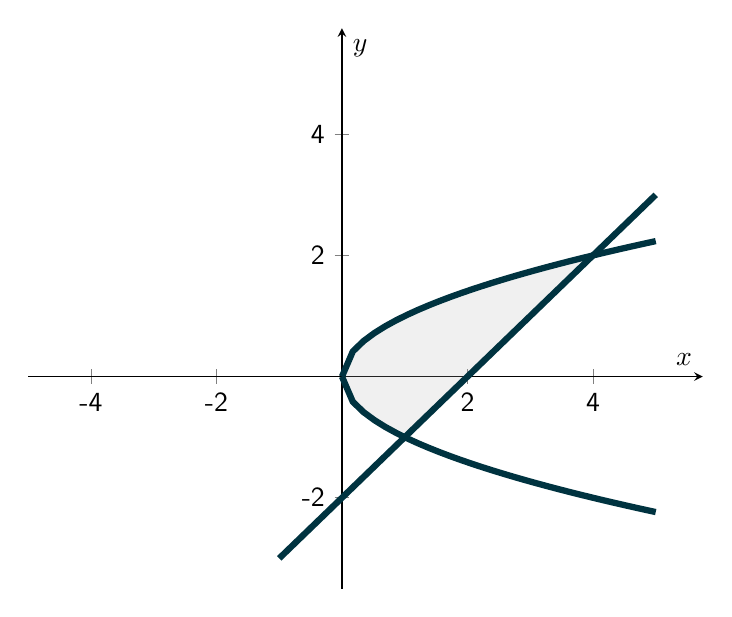
\begin{tikzpicture}[scale=1.25]
            \begin{axis}[
            axis lines = middle, very thick,
            xlabel = {$x$},
            ylabel = {$y$},
            xmin=-5, xmax=5.75,
            ymin=-3.5, ymax=5.75,
            xtick={-4,-2,0,2,4},
            xticklabels={-4,-2,0,2,4},
            ytick={-2,0,2,4},
            yticklabels={-2,0,2,4}        
            ]
            % Curves
            \addplot [name path = A,-,domain = 0:5, line width=0.8mm,DarkBlue,samples = 30] {sqrt(x)} ;
            \addplot [name path = B,-,domain = 0:5, line width=0.8mm,DarkBlue,samples = 30] {-sqrt(x)} ;
            \addplot [name path = C, line width=0.8mm, samples=4, smooth,domain=0:5, DarkBlue] coordinates {(-1,-3)(5,3)};
            % Fill area between paths
            \addplot [black!30, opacity=0.2] fill between [of = A and B, soft clip={domain=0:1}];
            \addplot [black!30, opacity=0.2] fill between [of = A and C, soft clip={domain=1:4}];
            \end{axis}
        \end{tikzpicture}    
    \end{center}   
        
    Thus
    \begin{align}
        \bar y &= \frac{M_x}M = \frac1M \int_{-1}^{2}\int_{y^2}^{y+2} 12y \, dx \, dy
    \end{align} 
    Thus
    \begin{align}
        a &= -1 \\
        b &= 2 \\
        c&= y^2 \\
        d&= y+2 \\
        f(x,y) &= \delta y = 12y
    \end{align}
    }
   \else

   \fi
    
\fi

\ifnum \Version=7
% SHORT SPHERICAL AND CYLINDRICAL EXERCISE
\part Point $P$ has rectangular (Cartesian) coordinates $(x,y,z) = (-6,0,8)$ in $\mathbb R^3$. In cylindrical coordinates, the point is $(r,\theta,z)$, and in spherical coordinates the point is $(\rho, \phi, \theta)$. Where $r=\framebox{\strut\hspace{1cm}}$, $\theta=\framebox{\strut\hspace{2cm}}$, $z=\framebox{\strut\hspace{1cm}}$, $\rho=\framebox{\strut\hspace{2cm}}$, and $\phi=\framebox{\strut\hspace{3cm}}$. 

    \ifnum \Solutions=1 {\color{DarkBlue} \textit{Solutions:} To convert to cylindrical we can use the equation $r^2 = x^2 + y^2$. 
    \begin{align}
        r^2 &= x^2 + y^2 = (-6)^2 + 0^2 = 36 \ \Rightarrow \ r = 6
    \end{align}
    To determine $\theta$ we can use $\tan\theta = y/x$. 
    \begin{align}
        \tan \theta &= \frac{y}{x} = \frac{0}{-6} = 0  \\
        \theta &= \arctan 0 
    \end{align} 
    The point in cylindrical is: 
    \begin{align}
        (r,\theta,z) &= (6,\pi,8) \\
        r &= 6 \\
        \theta &= \pi \\
        z &= 8
    \end{align}
    In spherical, we can start by obtaining $\rho$. 
    \begin{align}
        \rho^2 &= x^2+y^2+z^2\\
        \rho^2 &= (-6)^2 + 0^2 + 8^2 = 36+64 = 100 \\
        \rho &= 10
    \end{align}
    To obtain $\phi$ we can use the equation that relates $x$ to spherical. Using the expression for $x$, and the values that we already have for $x$, $\rho$ and $\theta$:
    \begin{align}
        x &= \rho \sin\phi \cos\theta \\
        -6 &= 10\sin\phi \cos(\pi) \\
        \sin\phi &= \frac{-6}{10 \cos(\pi)}  = \frac{6}{10}\\
        \phi &= \arcsin (6/10)
    \end{align}
    Our coordinates in spherical are
    \begin{align}
        \rho &= 10\\
        \phi &= \arcsin (6/10)\\
        \theta &= \pi
    \end{align}
    Note the following.
    \begin{itemize}
        \item We can, for this exercise, leave un-evaluated trig functions in the answer, because the question didn't specify that you should simplify your answer as much as possible. So it would be ok to leave your answer for $\theta$ as $\arctan 0$ or $\tan^{-1} 0$. 
        \item Our particular textbook uses the convention $(\rho, \phi, \theta)$, not $(\rho, \theta,\phi)$.
    \end{itemize}
    } 
    \else
      
    \fi
    
\fi





\ifnum \Version=8
% SHORT SPHERICAL AND CYLINDRICAL EXERCISE
\part Point $P$ has rectangular (Cartesian) coordinates $(x,y,z) = (4,4,7)$ in $\mathbb R^3$. In cylindrical coordinates, the point is $(r,\theta,z)$, and in spherical coordinates the point is $(\rho, \phi, \theta)$. Where $r=\framebox{\strut\hspace{1cm}}$, $\theta=\framebox{\strut\hspace{2cm}}$, $z=\framebox{\strut\hspace{1cm}}$, $\rho=\framebox{\strut\hspace{2cm}}$, and $\phi=\framebox{\strut\hspace{3cm}}$. 

    \ifnum \Solutions=1 {\color{DarkBlue} \textit{Solutions:} To convert to cylindrical we can use the equation $r^2 = x^2 + y^2$. 
    \begin{align}
        r^2 &= x^2 + y^2 = (4)^2 + 4^2 = 32 \ \Rightarrow \ r = \sqrt{32} = 4\sqrt2
    \end{align}
    It isn't necesssary to simplify to $4\sqrt2$. Then to determine $\theta$ we can use $\tan\theta = y/x$. 
    \begin{align}
        \tan \theta &= \frac{y}{x} = \frac{4}{4} = 1  \\
        \theta &= \arctan \pi/4
    \end{align} 
    The point in cylindrical is: 
    \begin{align}
        (r,\theta,z) &= (4\sqrt2,\pi/4,7) \\
        r &= 4\sqrt2 \\
        \theta &= \pi/4 \\
        z &= 7
    \end{align}
    In spherical, we can start by obtaining $\rho$. 
    \begin{align}
        \rho^2 &= x^2+y^2+z^2\\
        \rho^2 &= (4)^2 + 4^2 + 7^2 = 16+16+49 = 32+49 = 81 \\
        \rho &= 9
    \end{align}
    To obtain $\phi$ we can use the equation that relates $x$ to spherical. Using the expression for $x$, and the values that we already have for $x$, $\rho$ and $\theta$:
    \begin{align}
        x &= \rho \sin\phi \cos\theta \\
        4 &= 9\sin\phi \cos(\pi/4) \\
        \sin\phi &= \frac{4}{9 \cos(\pi/4)}  = \frac{4\sqrt2}{9}\\
        \phi &= \arcsin \left(\frac{4\sqrt2}{9}\right)
    \end{align}
    Note for $\phi$ we can also use:
    \begin{align}
        y &= \rho \sin\phi \sin\theta \\
        4 &= 9\sin\phi \sin(\pi/4) \\
        \sin\phi &= \frac{4}{9 \sin(\pi/4)}  = \frac{4\sqrt2}{9}\\
        \phi &= \arcsin \left(\frac{4\sqrt2}{9}\right)
    \end{align}    
    And we can also use:
    \begin{align}
        z &= \rho \cos\phi  \\
        7 &= 9\cos\phi  \\
        \sin\phi &= \frac{4}{9 \sin(\pi/4)}  = \frac{4\sqrt2}{9}\\
        \phi &= \arccos \left(\frac{7}{9}\right)
    \end{align}      
    Our coordinates in spherical are
    \begin{align}
        \rho &= 9\\
        \phi &= \arcsin \left(\frac{4\sqrt2}{9}\right), \ \textbf{or} \ \phi = \arccos(7/9)\\
        \theta &= \pi/4
    \end{align}
    Note the following.
    \begin{itemize}
        \item We can, for this exercise, leave un-evaluated trig functions in the answer, because the question didn't specify that you should simplify your answer as much as possible. So it would be ok to leave your answer for $\theta$ as $\arctan 1$ or $\tan^{-1} 1$. 
        \item Our particular textbook uses the convention $(\rho, \phi, \theta)$, not $(\rho, \theta,\phi)$.
    \end{itemize}
    } 
    \else
      
    \fi
    
\fi





% 15.6
% CENTROID Y-COORDINATE PARABOLA AND LINE
\ifnum \Version=9
    \part A thin plate with density $\delta=12$ is bounded in the $xy-$plane by $y=3-x^2$ and $y=1-x$. The plate has mass $M$. The $y-$coordinate of the centroid is $\bar y = M_x/M$, where $\displaystyle M_x = \int_A^B \int_C^D f(x,y) \, dy \, dx$,  and $A=\framebox{\strut\hspace{1cm}}$, $B=\framebox{\strut\hspace{1cm}}$, $C=\framebox{\strut\hspace{3cm}}$, $D=\framebox{\strut\hspace{3cm}}$, and $f(x,y) = \framebox{\strut\hspace{3cm}}$. 
    
    \ifnum \Solutions=1 
    {\color{DarkBlue}
    The region is bounded by 
    $$1-x \le y \le 3-x^2$$
    The given curves intersect when 
    \begin{align}
        1-x &= 3-x^2\\
        0 &= x^2-x-2 \\
        &= (x-2)(x+1)
    \end{align}
    The curves intersect at $x=-1,2$. Using $y=1-x$, the intersection points are $(-1,2)$ and $(2,-1)$. The region is shown below. 
    \begin{center}  
        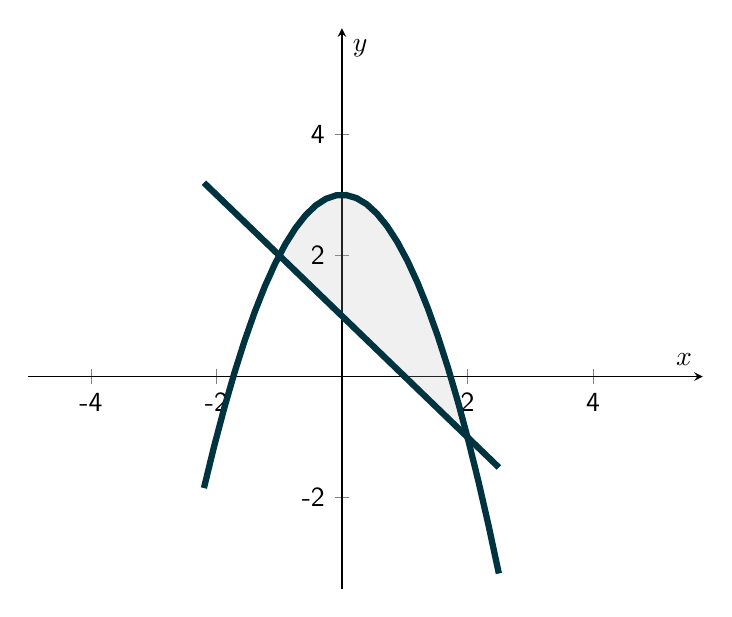
\begin{tikzpicture}[scale=1.25]
            \begin{axis}[
            axis lines = middle, very thick,
            xlabel = {$x$},
            ylabel = {$y$},
            xmin=-5, xmax=5.75,
            ymin=-3.5, ymax=5.75,
            xtick={-4,-2,0,2,4},
            xticklabels={-4,-2,0,2,4},
            ytick={-2,0,2,4},
            yticklabels={-2,0,2,4}        
            ]
            % Curves
            \addplot [name path = A,-,domain = -2.2:2.5, line width=0.8mm,DarkBlue,samples = 30] {3-x^2} ;
            \addplot [name path = C,-,domain = -2.2:2.5, line width=0.8mm,DarkBlue,samples = 4] {1-x} ;
            % Fill area between paths
            \addplot [black!30, opacity=0.2] fill between [of = A and C, soft clip={domain=-1:2}];
            \end{axis}
        \end{tikzpicture}    
    \end{center}   
        
    Thus
    \begin{align}
        \bar y &= \frac{M_x}M = \frac1M \int_{-1}^{2}\int_{1-x}^{3-x^2} 12y \, dy \, dx
    \end{align} 
    Thus
    \begin{align}
        A &= -1 \\
        B &= 2 \\
        C&= 1-x \\
        D&= 3-x^2 \\
        f(x,y) &= \delta y = 12y
    \end{align}
    }
   \else

   \fi
    
\fi
   
    % 13.3 and 13.4
% unit tangent vectors
% arc length
% curvature
% osculating circle
% unit normal

\ifnum \Version=1

\part The unit tangent vector for a curve $\mathbf r(t)$ is $\mathbf T(t) = \langle 0, \cos t, \sin t \rangle$. The unit normal vector is $\mathbf  N = \langle f(t), g(t), g(t) \rangle$, where $f(t) = \framebox{\strut\hspace{2cm}}$, $g(t) = \framebox{\strut\hspace{2cm}}$, $h(t) =\framebox{\strut\hspace{2cm}}$. 

\ifnum \Solutions=1 {\color{DarkBlue} \textit{Answer:} \textit{Solutions:} The normal vector is

\begin{align}
    \mathbf N &= \frac{d\mathbf T/dt}{|d\mathbf T/dt|} 
\end{align}
And
\begin{align}
    \mathbf T'(t) &= \langle 0,-\sin t, \cos t \rangle \\
    |\mathbf T'(t) | &= \sqrt{ 0 +(-\sin t)^2 + (\cos t)^2} =1\\
    \mathbf N &= \frac{d\mathbf T/dt}{|d\mathbf T/dt|} = \langle 0, - \sin(t),  \cos(t) \rangle
\end{align}
} 
\else
\fi        
\fi

\ifnum \Version=2

\part The velocity vector of an object moving on the curve $\mathbf r(t)$ is $\mathbf v(t) = \langle 4\cos (2t), 4\sin (2t) , 3 \rangle$ for $t>0$. The speed of the object for $t>0$ is $s(t) = |\mathbf v | = \framebox{\strut\hspace{1cm}}$. The unit tangent vector for $t>0$ is $\mathbf T = \langle f(t), g(t) , h(t) \rangle$, where $f(t) = \framebox{\strut\hspace{1.5cm}}$, $g(t) = \framebox{\strut\hspace{1.5cm}}$, $h = \framebox{\strut\hspace{1cm}}$. The curvature is $\kappa = \framebox{\strut\hspace{1cm}}$. 

\ifnum \Solutions=1 {\color{DarkBlue} \textit{Answer:} \textit{Solutions:} The speed is the magnitude of the given velocity vector and is
\begin{align}
    s &= |\mathbf v | =  \sqrt{(4\cos2t)^2 + (4\sin2t)^2 + 3^2 } = \sqrt{4^2 (\cos ^2 2 t + \sin^2 2t) + 3^2} = \sqrt{16 + 9} = 5
\end{align}
The unit tangent vector is 
\begin{align}
    \mathbf T &= \frac{\mathbf v}{|\mathbf v|} = \langle \frac{4}{5}\cos(2 t) , \frac 45 \sin (2t), \frac35 \rangle
\end{align}
For curvature we also need
\begin{align}
    \frac{d\mathbf T}{dt } &= \langle -\frac85 \sin 2t, \frac85 \cos 2t,0 \rangle \\
    \left | \frac{d\mathbf T}{dt } \right| &= \sqrt{ \left(-\frac85\sin 2t\right)^2 +   \left(\frac85 \cos 2 t\right)^2 } = \frac85
\end{align}
The curvature is
\begin{align}
    \kappa = \frac{1}{|\mathbf v |}\left| \frac{d\mathbf T}{dt}\right| = \frac{1}{5} \cdot \frac{8}{5} = \frac{8}{25}
\end{align}
} 
\else
\fi        
\fi


\ifnum \Version=3

\part A plane curve $\mathbf r(t)$ has curvature $\kappa = \frac{1}{8}$ at $\mathbf r(t_0) = \langle 15, 2 \rangle$, and the unit normal vector at $t=t_0$ is $\mathbf  N = \mathbf j = \langle 0, 1 \rangle$. The equation of the osculating circle at $t=t_0$ is \framebox{\strut\hspace{3.5cm}}.

\ifnum \Solutions=1 {\color{DarkBlue} \textit{Answer:} \textit{Solutions:} Recall that The circle of curvature, or osculating circle, at a point $P$ on a plane curve where $\kappa \ne 0$ is the circle in the plane of the curve that

\begin{enumerate}
    \item is tangent to the curve at P (has the same tangent line the curve has)
    \item has the same curvature the curve has at P
    \item lies toward the concave or inner side of the curve
\end{enumerate}
The \textbf{radius of curvature} of the curve at P is the radius of the circle of curvature, which is $\frac{1}{\kappa}$. So to obtain the radius, we calculate $\kappa$ and take the reciprocal. The \textbf{center} of the osculating circle of the curve at P lies on the inner side of the curve, and the unit normal points in the direction of the inner side of the planar curve. 

So for this problem we have a circle with radius $1/\kappa = 8$, and whose centre is 8 units away from the point $(15,2)$ in the direction of $\mathbf N$. The circle has equation
$$(x-15)^2 + (y-10)^2 = 8^2$$
} 
\else
  
\fi        
\fi




\ifnum \Version=4

\part The velocity vector for an object moving on the curve $\mathbf r(t)$ is $\mathbf v(t) = \langle t\cos t, t\sin t \rangle$. The speed of the object for $t>0$ is $s(t) = \framebox{\strut\hspace{1cm}}$. The unit tangent vector for $t>0$ is $\mathbf T = \langle f(t), g(t) \rangle$, where $f(t) = \framebox{\strut\hspace{2cm}}$, $g(t) = \framebox{\strut\hspace{2cm}}$. 

\ifnum \Solutions=1 {\color{DarkBlue} \textit{Answer:} \textit{Solutions:} The speed is the magnitude of the velocity vector and is
\begin{align}
    s &= |\mathbf v | = \sqrt{(t\cos t)^2 + (t\sin t)^2 } = \sqrt{t^2 (\cos ^2 t + \sin^2 t)} = |t|
\end{align}
But we are told that $t>0$ so we can use $|t| = t$. The unit tangent vector is 
\begin{align}
    \mathbf T &= \frac{\mathbf v}{|\mathbf v|} = \langle \cos t, \sin t \rangle
\end{align}
} 
\else
\fi        
\fi

\ifnum \Version=5

\part A plane curve $\mathbf r(t)$ has curvature $\kappa = \frac{1}{4}$ at the point $\mathbf r(t_0) = 3\mathbf i + 5\mathbf j$, and the unit normal vector at $t_0$ is $\mathbf  N = \mathbf i = \langle1,0\rangle$. The equation of the osculating circle at $t=t_0$ is \framebox{\strut\hspace{3.5cm}}.

\ifnum \Solutions=1 {\color{DarkBlue} \textit{Answer:} \textit{Solutions:} Recall that The circle of curvature, or osculating circle, at a point $P$ on a plane curve where $\kappa \ne 0$ is the circle in the plane of the curve that

\begin{enumerate}
    \item is tangent to the curve at P (has the same tangent line the curve has)
    \item has the same curvature the curve has at P
    \item lies toward the concave or inner side of the curve
\end{enumerate}
The \textbf{radius of curvature} of the curve at P is the radius of the circle of curvature, which is $\frac{1}{\kappa}$. So to obtain the radius, we calculate $\kappa$ and take the reciprocal. The \textbf{center} of the osculating circle of the curve at P lies on the inner side of the curve, and the unit normal points in the direction of the inner side of the planar curve. 

So for this problem we have a circle with radius $1/\kappa = 4$, and whose centre is 4 units away from the point $(3,5)$ in the direction of $\mathbf N$. The circle has equation
$$(x-7)^2 + (y-5)^2 = 4^2$$
} 
\else
  
\fi        
\fi


\ifnum \Version=6

\part The velocity vector for an object moving on the curve $\mathbf r(t)$ is $\mathbf v(t) = \langle 4t\cos t, 4t\sin t \rangle$ for $t>0$. The speed of the object for $t>0$ is $s(t)  = |\mathbf v | = \framebox{\strut\hspace{1cm}}$. The unit tangent vector for $t>0$ is $\mathbf T = \langle f(t), g(t) \rangle$, where $f(t) = \framebox{\strut\hspace{1.5cm}}$, $g(t) = \framebox{\strut\hspace{1.5cm}}$. The curvature is $\kappa = \framebox{\strut\hspace{1cm}}$. 

\ifnum \Solutions=1 {\color{DarkBlue} \textit{Answer:} \textit{Solutions:} The speed is the magnitude of the given velocity vector and is
\begin{align}
    s &= |\mathbf v | =  \sqrt{(4t\cos t)^2 + (4t\sin t)^2 } = \sqrt{4^2t^2 (\cos ^2 t + \sin^2 t)} = 4|t|
\end{align}
But we are told that $t>0$ so we can assume $|t| = t$. The unit tangent vector is 
\begin{align}
    \mathbf T &= \frac{\mathbf v}{|\mathbf v|} = \langle \cos t, \sin t \rangle
\end{align}
We need
\begin{align}
    \frac{d\mathbf T}{dt } &= \langle -\sin t, \cos t \rangle \\
    \left | \frac{d\mathbf T}{dt } \right| &= \sqrt{ (-\sin t)^2 +   \cos^2 t } = 1
\end{align}
The curvature is
\begin{align}
    \kappa = \frac{1}{|\mathbf v |}\left| \frac{d\mathbf T}{dt}\right| = \frac{1}{4t} 
\end{align}
} 
\else
\fi        
\fi



\ifnum \Version=7

\part The velocity vector of an object moving on the curve $\mathbf r(t)$ is $\mathbf v(t) = \langle 3\cos (2t), 3\sin (2t) \rangle$ for $t>0$. The speed of the object for $t>0$ is $s(t) = |\mathbf v | = \framebox{\strut\hspace{1.5cm}}$. The unit tangent vector for $t>0$ is $\mathbf T = \langle f(t), g(t)  \rangle$, where $f(t) = \framebox{\strut\hspace{2cm}}$, and $g(t) = \framebox{\strut\hspace{2cm}}$.  The curvature for $t>0$ is \framebox{\strut\hspace{1.5cm}}. 

\ifnum \Solutions=1 {\color{DarkBlue} \textit{Answer:} \textit{Solutions:} The speed is the magnitude of the given velocity vector and is
\begin{align}
    s &= |\mathbf v | =  \sqrt{(3\cos t)^2 + (3\sin t)^2  } = \sqrt{3^2 (\cos ^2 t + \sin^2 t) + 3^2} = \sqrt{ 9} = 3
\end{align}
The unit tangent vector is 
\begin{align}
    \mathbf T &= \frac{\mathbf v}{|\mathbf v|} 
    = \langle \frac{3}{3}\cos(2 t) , \frac 33 \sin (2t) \rangle 
    = \langle \cos(2 t) ,  \sin (2t) \rangle
\end{align}
For curvature we also need
\begin{align}
    \frac{d\mathbf T}{dt } &= \langle -2 \sin 2t, 2 \cos 2t\rangle \\
    \left | \frac{d\mathbf T}{dt } \right| &= \sqrt{ \left(-2\sin 2t\right)^2 +   \left(2 \cos 2 t\right)^2 } = 2
\end{align}
The curvature is
\begin{align}
    \kappa = \frac{1}{|\mathbf v |}\left| \frac{d\mathbf T}{dt}\right| = \frac{1}{3} \cdot 2 = \frac{2}{3}
\end{align}
} 
\else
\fi        
\fi


\ifnum \Version=8

\part A plane curve $\mathbf r(t)$ has curvature $\kappa = \frac{1}{4}$ at $\mathbf r(t_0) = \langle 5, 3 \rangle$, and the unit normal vector at $t=t_0$ is $\mathbf  N = \mathbf j = \langle 0, 1 \rangle$. The equation of the osculating circle at $t=t_0$ is \framebox{\strut\hspace{3.5cm}}.

\ifnum \Solutions=1 {\color{DarkBlue} \textit{Answer:} \textit{Solutions:} Recall that The circle of curvature, or osculating circle, at a point $P$ on a plane curve where $\kappa \ne 0$ is the circle in the plane of the curve that

\begin{enumerate}
    \item is tangent to the curve at P (has the same tangent line the curve has)
    \item has the same curvature the curve has at P
    \item lies toward the concave or inner side of the curve
\end{enumerate}
The \textbf{radius of curvature} of the curve at P is the radius of the circle of curvature, which is $\frac{1}{\kappa}$. So to obtain the radius, we calculate $\kappa$ and take the reciprocal. The \textbf{center} of the osculating circle of the curve at P lies on the inner side of the curve, and the unit normal points in the direction of the inner side of the planar curve. 

So for this problem we have a circle with radius $1/\kappa = 4$, and whose centre is 4 units away from the point $(5,3)$ in the direction of $\mathbf N$. The circle has equation
$$(x-5)^2 + (y-7)^2 = 4^2$$
} 
\else
  
\fi        
\fi






\ifnum \Version=9

\part The velocity vector of an object moving on the curve $\mathbf r(t)$ is $\mathbf v(t) = \langle t, 3 \rangle$ for $t>0$. The speed of the object at $t=2$ is $s(2) = |\mathbf v(2) | = \framebox{\strut\hspace{1.75cm}}$. The unit tangent vector at $t=2$ is $\mathbf T(2) = \langle c_1 ,c_2  \rangle$, where $c_1 = \framebox{\strut\hspace{1.75cm}}$, $c_2 = \framebox{\strut\hspace{1.75cm}}$. The curvature is $\framebox{\strut\hspace{1.75cm}}$. 

\ifnum \Solutions=1 {\color{DarkBlue} \textit{Answer:} \textit{Solutions:} The speed is the magnitude of the given velocity vector and is
\begin{align}
    s &= |\mathbf v | =  \sqrt{( t)^2 + (3)^2  } = \sqrt{t^2+9}\\
    s(2) &= \sqrt{2^2+9} = \sqrt{13}
\end{align}
We also need the unit tangent vector at $t=2$. 
\begin{align}
    \mathbf T (t) &= \frac{\mathbf v}{|\mathbf v|} = \frac{t\mathbf i + 3\mathbf j}{\sqrt{t^2+9}} \\
    \mathbf T (2) &= \frac{2\mathbf i + 3\mathbf j}{\sqrt{2^2+9}}  
    = \langle \frac{2}{\sqrt{13}} , \frac {3}{\sqrt{13}}  \rangle \\
    c_1 &= \frac{2}{\sqrt{13}}\\
    c_2 &= \frac{3}{\sqrt{13}}
\end{align}
The curvature is zero because the motion is along a straight line. 
\begin{align}
    \kappa = 0
\end{align}
} 
\else
\fi        
\fi

\ifnum \Version=10

\part A plane curve $\mathbf r(t)$ has curvature $\kappa = \frac{1}{10}$ at $\mathbf r(t_0) = \langle 5, 0 \rangle$, and the unit normal vector at $t=t_0$ is $\mathbf  N = \mathbf j = \langle 0, 1 \rangle$. The equation of the osculating circle at $t=t_0$ is \framebox{\strut\hspace{3.5cm}}.

\ifnum \Solutions=1 {\color{DarkBlue} \textit{Answer:} \textit{Solutions:} Recall that The circle of curvature, or osculating circle, at a point $P$ on a plane curve where $\kappa \ne 0$ is the circle in the plane of the curve that

\begin{enumerate}
    \item is tangent to the curve at P (has the same tangent line the curve has)
    \item has the same curvature the curve has at P
    \item lies toward the concave or inner side of the curve
\end{enumerate}
The \textbf{radius of curvature} of the curve at P is the radius of the circle of curvature, which is $\frac{1}{\kappa}$. So to obtain the radius, we calculate $\kappa$ and take the reciprocal. The \textbf{center} of the osculating circle of the curve at P lies on the inner side of the curve, and the unit normal points in the direction of the inner side of the planar curve. 

So for this problem we have a circle with radius $1/\kappa = 10$, and whose centre is 10 units away from the point $(5,0)$ in the direction of $\mathbf N$. The circle has equation
$$(x-5)^2 + (y-10)^2 = 10^2$$
} 
\else
  
\fi        
\fi
   
\end{parts}

\newpage \question[0.25] \ID
% CHANGE OF VARIABLE (15.8)
% OR APPLICATION (15.6)
% OR TRIPLE CARTESIAN (15.5) 

\ifnum \Version=1
% CENTROID
% BASED ON THOMAS EXERCISES, 15.6 #1
% SUFFICIENT FOR A PRACTICE EXAM
\question[6] A thin plate of density $\delta(x,y) = 12x$ is bounded by the lines $x = 0, y = x$, and the parabola $y = x^2-6$ in the first quadrant. 
\begin{parts} 
    \part Determine the mass of the plate, $M$. Please show your work. 
    \ifnum \Solutions=1 
    {\color{DarkBlue} \textit{Solutions:}
    Curves intersect when $$x = x^2-6 \quad \Rightarrow \quad 0 = x^2 - x - 6 = (x-3)(x+2)$$
    Or $x=3, -2$. We can ignore $x=-2$ because the region is the first quadrant. Curves intersect at the point $(3,3)$, and 
    \begin{align}
        0 \le y \le 3, \quad y \le x \le \sqrt{y+6}
    \end{align}
    The mass is
    \begin{align}
        M &= \int_0^3 \int_y^{\sqrt{y+6}} \delta \, dx \, dy \\
        &= \int_0^3 \int_y^{\sqrt{y+6}} 12x \, dx \, dy \\
        &= \int_0^3  \left. 6x^2 \right|_{x=y}^{x=\sqrt{y+6}} \, dy \\
        &= \int_0^3 6(y + 6 - y^2) \, dy \\
        &= \int_0^3 6y + 36 - 6y^2 \, dy \\
        &= \left. (3y^2 + 36y - 2y^3 ) \right|_0^3 \, dy \\
        &= 27 + 108 - 54 \\
        &= 81
    \end{align}
    }
    \else 
    \vspace{16cm}
    \fi
    \part Use your results from the previous part to set up an integral that can be used to determine the $x-$coordinate of the center of mass of the plate. You do not need to evaluate your integral. 
    \ifnum \Solutions=1 {\color{DarkBlue} \textit{Solutions:} the $x-$coordinate of the center of mass, $\bar x$, is
    \begin{align}
    \bar x &= \frac{M_y}{M} = \frac{1}{81} \int_0^3 \int_y^{\sqrt{y+6}} 12x^2 \, dx \, dy 
    \end{align}
    } 
    \else
      
    \fi
    \end{parts} 
\fi
    





\ifnum \Version=2
% LONGISH CHANGE OF VARIABLE
% VERBATUM FROM SPRING 2022 QUIZ
% hand written solution only
% SUFFICIENT FOR A PRACTICE EXAM
\question[6] Consider the double integral

$$I=\iint_R \frac{x+2y}{2y-x} dA$$

where $R$ is the parallelogram with vertices $(-3,1), (-1,0), (-1,2), (1,1)$. Our goal is to determine the area of the parallelogram using the transform below. 
$$u=x+2y, \qquad v = -x +2y$$ 
Please show your work for the following. 
\begin{parts} 
    \part Use the given transform to calculate the Jacobian of the transform, $J = \partial x(u,v)/\partial y(u,v)$. 
    \ifnum \Solutions=1 
    \else 
    \vspace{8 cm}
    \fi
    \part Use your results from Part (a) and the given transform to transform the double integral. You do not need to evaluate your integral. 
\end{parts} 

\ifnum \Solutions=1 {\color{DarkBlue} \textit{Solutions:} the integral after the transform is $$\displaystyle \frac14 \int_1^5\int_{-1}^3 \frac uv \, du \, dv$$
A screen capture of a hand-written solution from a previous offer of MATH 2551 is below. 
    \begin{figure}[h]
    \centering
    \includegraphics[width=16cm]{202302/Exam3/Images/ImgE3.OR.06.png}
    \end{figure}  
    
    } 
   \else
      
   \fi
    
\fi

\ifnum \Version=3
% CENTROID
% BASED ON THOMAS EXERCISES, 15.6 #1
% SUFFICIENT FOR A PRACTICE EXAM
\question[6] A thin plate with density $\delta(x,y) = 24y$ is bounded by the lines $x = 0, x=2y$, and the parabola $x=y^2$ in the first quadrant. 
\begin{parts} 
    \part Determine the mass of the plate, $M$. Please show your work. 
    
    \ifnum \Solutions=1 
    {\color{DarkBlue} \textit{Solutions:}
    Curves intersect when $$2y = y^2 \quad \Rightarrow \quad 0 = y^2-2y = y(y-2)$$
    Or $y=0,2$. Curves intersect at the points $(0,0)$, $(4,2)$. 
    The mass is
    \begin{align}
        M = \int_0^4 \int_{x/2}^{\sqrt{x}} \delta \, dy \, dx 
        &= \int_0^4 \int_{x/2}^{\sqrt{x}} 24y \, dy \, dx \\
        &= \int_0^4  \left. 12y^2 \right|_{y=x/2}^{y=\sqrt{x}} \, dx \\
        &= 12 \int_0^4 (x-\frac{x^2}{4}) \, dx \\
        &= 12 \left. (\frac{x^2}{2} - \frac{x^3}{12} ) \right|_0^4 \, dy \\
        &= 12 (\frac{16}{2} - \frac{64}{12}) \\
        &= 96 - 64\\
        &= 32
    \end{align}
    \textbf{An Alternate Solution}\\
    Another way to approach this problem is to use the integration order $dx\,dy$. In this case the double integral becomes
    \begin{align}
        M = \int_0^2 \int_{y^2}^{2y} \delta \, dx \, dy
        &= \int_0^2 \int_{y^2}^{2y} 24y \, dx \, dy \\
        &= 24\int_0^2  \left. yx \right|_{x=y^2}^{x=2y} \, dy \\
        &= 24 \int_0^2 (2y^2 - y^3) \, dy \\
        &= 24 \left. (\frac{2y^3}{3} - \frac{y^4}{4} ) \right|_0^2 \, dy \\
        &= 24 (\frac{16}{3} - \frac{16}{4}) \\
        &= \frac{24\cdot16}{3} - 24\cdot 4 \\
        &= 8\cdot16 - 96 \\
        &= 128 - 96 \\
        &= 32
    \end{align}    
    }
    \else 
    \vspace{14cm}
    \fi
    \part Use your results from the previous part to set up an integral that can be used to determine the $x-$coordinate of the center of mass of the plate. You do not need to evaluate your integral. 
    \ifnum \Solutions=1 {\color{DarkBlue} \textit{Solutions:} the $x-$coordinate of the center of mass, $\bar x$, is
    \begin{align}
    \bar x &= \frac{M_y}{M} = \frac{1}{32} \int_0^4 \int_{x/2}^{\sqrt{x}} 24xy \, dy \, dx
    \end{align}
    \textbf{An Alternate Solution}\\    
    It is also ok to use the integration order $dx\,dy$. In this case the double integral becomes
    \begin{align}
    \bar x &= \frac{M_y}{M} = \frac{1}{32} \int_0^2 \int_{y^2}^{2y} 24xy \, dx \, dy 
    \end{align}
    } 
    \else
      
    \fi
    \end{parts} 
\fi

\ifnum \Version=4
% VERSION B
% LONG CHANGE OF VARIABLE
% BASED ON AN EXAMPLE FROM THOMAS
% SECTION 15.8 FROM THOMAS
\question[6] Consider the double integral

$$I= 9 \iint_R (y-2x)^2 \sqrt{x+y} \, dA$$

where $R$ is the region in the first quadrant bounded by the lines $x=0$, $y=0$, and $y=1-x$. Our goal is to determine the area of $R$ using the transform below. 
$$u=x+y, \qquad v = y-2x$$ 
Please show your work for the following. 
\begin{parts} 
    \part Use the given transform to calculate the Jacobian of the transform, $J = \partial x(u,v)/\partial y(u,v)$. 
    \ifnum \Solutions=1 {\color{DarkBlue} \textit{Solutions:} Solving for $x$ and $y$ using an augmented matrix,
    \begin{align}
        \begin{pmatrix} 1 & 1 & u \\-2 & 1 & v\end{pmatrix} 
        \sim \begin{pmatrix} 1 & 1 & u \\0 & 3 & 2u+v\end{pmatrix} 
        \sim \begin{pmatrix} 1 & 0 & u/3 - v/3 \\0 & 1 & 2u/3+v/3 \end{pmatrix} 
    \end{align}
    Thus
    \begin{align}
        x &= \frac13(u-v), \ y = \frac13(2u+v) \\
        J(u,v) & = \begin{vmatrix} \DXDU & \DXDV \\[8pt] \DYDU & \DYDV \end{vmatrix} = \begin{vmatrix} 1/3 & -1/3 \\ 2/3 & 1/3 \end{vmatrix} = 1/9 + 2/9 = 1/3
    \end{align}
    }
    \else 
    \vspace{8 cm}
    \fi
    \part Use the given transform and your results from Part (a) to convert the double integral into a double integral over a region in the $uv-$plane. You do not need to evaluate your integral. 
    \ifnum \Solutions=1 {\color{DarkBlue} \textit{Solutions:} Converting each of the boundaries in the $xy-$plane into the $uv-$plane we obtain
        \begin{align}
            x+y &= 1 \quad \Rightarrow \quad \frac13(u-v) + \frac13(2u+v) = 1 &&\Rightarrow \quad u = 1\\
            x&=0 \quad \Rightarrow \quad \frac13(u-v) = 0 &&\Rightarrow \quad v = u\\
            y&= 0 \quad \Rightarrow \quad \frac13(2u+v) = 0 &&\Rightarrow \quad v = -2u
        \end{align}
        The region is described by either of the following relations:
        \begin{align}
            S_1: & \quad 0 \le u \le 1, \quad -2u \le v \le u \\
            S_2: & \quad -2 \le v \le 0, \quad -v/2 \le u \le 1, \ \text{and } 0 \le v \le 1, \quad v \le u \le 1
        \end{align}
        The first set of inequalities requires only a single double integral, but it is ok to set up two double integrals. If using $S_1$, we use $dv\,du$ and obtain
        \begin{align}
            I= 9 \iint_R (y-2x)^2 \sqrt{x+y} \, dA = 9 \int_0^1 \int_{-2u}^u v^2u^{1/2} \frac13 \,dv\,du
        \end{align}
        If using $S_2$, we use $du\,dv$ and obtain
        \begin{align}
            I= 9 \iint_R (y-2x)^2 \sqrt{x+y} \, dA 
            = 9 \int_{-2}^0 \int_{-v/2}^1 v^2u^{1/2} \frac13 \,du\,dv
            + 9 \int_{0}^1 \int_{v}^1 v^2u^{1/2} \frac13 \,du\,dv
        \end{align}        
        } 
       \else
          
       \fi
    \end{parts} 

    \fi



\ifnum \Version=5
    % USE FOR VERSION B
    % LONG CYLINDRICAL WITH APPLICATION TO MASS WITH VARYING DENSITY
    % FROM 15.8
    \question[6] An object $D$ lying in the first octant is bounded below by the $xy-$plane, above by the plane $z=3+4y$, and by the cylinder $x^2+y^2 = 4$. The density of the object at any point in $D$ is equal to the distance from the point to the $z$-axis.  Please show your work for the following.
    
    \begin{parts} 
    \part Use cylindrical coordinates to calculate the total of mass of the object, $M$. Please show your work. 
    
    \ifnum \Solutions=1 {\color{DarkBlue} The object is only in the first octant so $$0 \le \theta \le \pi/2$$ Using $\delta = \sqrt{x^2+y^2} = r$, the $z-$coordinate of the center of mass is computed using 
    \begin{align}
        M &= \iiint_D  \delta \, dV \\
        &= \int_0^{\pi/2} \int_0^2 \int_0^{3+4r\sin\theta}  \delta(r,\theta) \, r\, dz\,dr\,d\theta\\
        &= \int_0^{\pi/2} \int_0^2 \int_0^{3+4r\sin\theta}   r^2 \, dz\,dr\,d\theta\\
        &= \int_0^{\pi/2} \int_0^2    r^2 \, (3+4r\sin\theta) \,dr\,d\theta \\
        &= \int_0^{\pi/2} \int_0^2     \, (3r^2+4r^3\sin\theta) \,dr\,d\theta \\
        &= \int_0^{\pi/2}  \left. \, (r^3+r^4\sin\theta) \right|_{r=0}^{r=2} d\theta \\
        &= \int_0^{\pi/2}  (8 + 16\sin\theta) d\theta \\
        &=  \left. (8\theta - 16\cos\theta) \right|_0^{\pi/2} \\
        &=  (4\pi - 0) - (0 - 16) \\
        &= 4\pi + 16
    \end{align}
    
    } 
    \else
        \vspace{14cm}
    \fi
    
    \part Use your results from the previous part to set up a triple integral in cylindrical coordinates that can be used to determine the $z-$coordinate of the center of mass of the object. You do not need to evaluate your integral. 

    \ifnum \Solutions=1 {\color{DarkBlue} \textit{Solutions:} the $z-$coordinate of the center of mass, $\bar x$, is
    \begin{align}
    \bar z &= \frac{M_{xy}}{M} = \frac{1}{16\pi+16} \int_0^{\pi/2} \int_0^2 \int_0^{3+4r\sin\theta}  z \, \delta(r,\theta) \, r\, dz\,dr\,d\theta
    \end{align}
    } 
    \else
      
    \fi
    \end{parts} 
\fi


% TRANSFORM: SOLVE FOR X & Y, BOUNDARIES, EVALUATE, TRIANGLES
% VERSION A
\ifnum \Version=6
    \question[6] Consider the transform $u=x+y$ and $v=4x+5y$, and the integral $\displaystyle I = \iint_{R}  \,dxdy$. Region $R$ is the triangle in the $xy$-plane bounded by $x+y=0$, $4x+5y=0$, $6x+7y=4$. The transform maps $R$ to region $G$ in the $uv-$plane.  Please show your work for the following.

    \begin{enumerate}
        \item[a)] Solve the system, $u=x+y$ and $v=4x+5y$, for $x$ and $y$ in terms of $u$ and $v$.
            \ifnum \Solutions=1 {\color{DarkBlue} \\[12pt] 
            \textbf{Solutions:}
            We can use the expressions for $u$ and $v$ as an augmented matrix and row reduce. 
            \begin{align}
                \begin{pmatrix} 1 & 1 & u \\ 4 & 5 & v\end{pmatrix} 
                \sim \begin{pmatrix} 1 & 1 & u \\0 & 1 & v - 4u \end{pmatrix} 
                \sim \begin{pmatrix} 1 & 0 & 5u - v \\ 0 & 1 & v - 4u \end{pmatrix} 
            \end{align}
            Thus $x = 5u - v$, and $y = v - 4u$. 
            } 
            \else 
            \vspace{5cm}
            \fi
        \item[b)] Transform the boundaries of $R$ to the $uv-$plane. In other words, determine the boundaries of $G$ in terms of $u$ and $v$. 
            \ifnum \Solutions=1 {\color{DarkBlue} \\[12pt] 
            \textbf{Solutions:} the three lines are transformed below. 
            \begin{itemize}
                \item The line $x+y=0$ becomes $u=0$. 
                \item The line $4x+5y=0$ becomes $v=0$. 
                \item The line $6x+7y=4$ is: 
                \begin{align}
                    6x+7y &=4 \\
                    6\cdot(5u-v) + 7\cdot(v-4u) &= 4\\
                    30u -28u -6v+7v &=4 \\
                    v &= 4 -2u
                \end{align}
            \end{itemize}
            } 
        \else 
        \vspace{5cm}
        \fi        
            
        \item[c)] Use the given transformation and your results from parts (a) and (b) to set up a double integral that in the $uv-$plane that is equal to $I$. Do not evaluate the integral. You also do not need to calculate the Jacobian and may use that the Jacobian of the transform is $J(u,v) = 1$.
            \ifnum \Solutions=1 {\color{DarkBlue} \\[12pt] 
            \textbf{Solutions:}
            \begin{align}
                \iint_{R} \,dx\,dy
                &= \iint_{G}  \left| J(u,v) \right| \,dv\,du 
                = \int_0^2\int_{0}^{4-2u}  \left| 1 \right| \,dv\,du 
                = \int_0^2\int_{0}^{4-2u} \,dv\,du
            \end{align}
            Note the following.
            \begin{itemize}
                \item We did not need to compute the Jacobian but it is computed as follows. 
                $$J 
                = \begin{vmatrix} x_u & x_v \\ y_u & y_v \end{vmatrix} 
                = \begin{vmatrix} 5 & -1 \\ -4 & 1\end{vmatrix} 
                = 5 - 4
                = 1$$
                \item             We did not need to evaluate the integral but if we did:
            \begin{align}
                I = \int_0^2\int_{0}^{4-2u}  \left| 1 \right| \,dv\,du
                = 1 \int_0^2 (4-2u) \,du
                =  \left. 4u - u^2 \right|_0^2 
                = 4
            \end{align}
            \item It is also ok to use the other integration order: $I = \int_0^4\int_0^{2-v/2} \, du \, dv$.
            \end{itemize}
            } 
            \else 
            \fi        
    \end{enumerate}
 
\fi 



% TRANSFORM: SOLVE FOR X & Y, BOUNDARIES, EVALUATE, PARALLELOGRAM
% VERSION A
\ifnum \Version=7
    \question[6] Consider the integral $\displaystyle I = 2\iint_{R} x-4y \,dx\,dy$, where $R$ is the parallelogram in the $xy$-plane bounded by $x-4y=2$, $x-4y=1$, $3y-x=3$, $3y-x=6$. Suppose the transform $u=x-4y$ and $v=3y-x$, maps region $R$ to region $G$ in the $uv-$plane.  Please show your work for the following.

    \begin{enumerate}
        \item[a)] Solve the system, $u=x-4y$ and $v=3y-x$, for $x$ and $y$ in terms of $u$ and $v$.
            \ifnum \Solutions=1 {\color{DarkBlue} \\[12pt] 
            \textbf{Solutions:}
            We can use the expressions for $u$ and $v$ as an augmented matrix and row reduce. 
            \begin{align}
                \begin{pmatrix} 1 & -4 & u \\ -1 & 3 & v\end{pmatrix} 
                \sim \begin{pmatrix} 1 & -4 & u \\0 & -1 & v + u\end{pmatrix} 
                \sim \begin{pmatrix} 1 & 0 & -3u-4v\\0 & 1 & -u-v\end{pmatrix} 
            \end{align}
            Thus
            \begin{align}
                x &=  -3u-4v\\
                y &= -u-v
            \end{align}

            } 
            \else 
            \vspace{5cm}
            \fi
        \item[b)] Transform the boundaries of $R$ to the $uv-$plane. In other words, determine the boundaries of $G$ in terms of $u$ and $v$. 
            \ifnum \Solutions=1 {\color{DarkBlue} \\[12pt] 
            \textbf{Solutions:} the four lines are transformed below. 
            \begin{itemize}
                \item The line $x-4y=2$ becomes $u=2$. 
                \item The line $x-4y=1$ becomes $u=1$. 
                \item The line $3y-x=3$ becomes $v=3$. 
                \item The line $3y-x=6$ becomes $v=6$. 
            \end{itemize}
            } 
        \else 
        \vspace{5cm}
        \fi        
            
        \item[c)] Use the given transformation and your results from parts (a) and (b) to set up a double integral that in the $uv-$plane that is equal to $I$. Do not evaluate the integral. You also do not need to calculate the Jacobian and may use that the Jacobian of the transform is  $J(u,v) = -1$. 
            \ifnum \Solutions=1 {\color{DarkBlue} \\[12pt] 
            \textbf{Solutions:}
            \begin{align}
                \iint_{R} 2x-8y \,dx\,dy
                = \iint_{G} 2u \left| J(u,v) \right| \,du\,dv
                = \int_3^6\int_{1}^2 2u \left| -1 \right| \,du\,dv
                = \int_3^6\int_{1}^2 2u \,du\,dv
            \end{align}
            Note the following.
            \begin{itemize}
                \item We did not need to evaluate the integral, but if we did: 
                \begin{align}
                \iint_{R} 2x-8y \,dx\,dy
                &= \iint_{G} 2u \left| J(u,v) \right| \,du\,dv\\
                &= \int_3^6\int_{1}^2 2u \left| -1 \right| \,du\,dv\\
                &= \int_3^6\left. u^2 \right|_{1}^2 \,dv\\
                &= \int_3^6 3 \,dv\\
                &= 3 \cdot(6 -3) \\
                &= 9
            \end{align}
            \end{itemize}
            } 
            \else 
            \fi        
    \end{enumerate}
 
\fi 




% TRANSFORM: SOLVE FOR X & Y, BOUNDARIES, EVALUATE
% VERSION B
\ifnum \Version=8
    \question[6] Consider the transform $u=x-y$ and $v=4y-2x$, and the integral $\displaystyle I = \iint_{R} \,dxdy$, where $R$ denotes the triangle in the $xy$-plane bounded by $x-y=2$, $4y-2x=0$, $3y=2x$. The transform maps region $R$ to region $G$ in the $uv-$plane.  Please show your work for the following.

    \begin{enumerate}
        \item[a)] Solve the system, $u=x-y$ and $v=4y-2x$, for $x$ and $y$ in terms of $u$ and $v$.
            \ifnum \Solutions=1 {\color{DarkBlue} \\[12pt] 
            \textbf{Solutions:}
            We can use the expressions for $u$ and $v$ as an augmented matrix and row reduce. 
            \begin{align}
                \begin{pmatrix} 1 & -1 & u \\ -2 & 4 & v\end{pmatrix} 
                \sim \begin{pmatrix} 1 & -1 & u \\0 & 2 & v + 2u\end{pmatrix} 
                \sim \begin{pmatrix} 1 & -1 & u\\0 & 1 & u+v/2\end{pmatrix} 
                \sim \begin{pmatrix} 1 & 0 & 2u+v/2\\0 & 1 & u+v/2\end{pmatrix} 
            \end{align}
            Thus $x = 2u+v/2$, and $y = u + \frac{v}{2}$. 
            } 
            \else 
            \vspace{5cm}
            \fi
        \item[b)] Transform the boundaries of $R$ to the $uv-$plane. In other words, determine the boundaries of $G$ in terms of $u$ and $v$. 
            \ifnum \Solutions=1 {\color{DarkBlue} \\[12pt] 
            \textbf{Solutions:} the three lines are transformed below. 
            \begin{itemize}
                \item The line $x-y=2$ becomes $u=2$. 
                \item The line $4x-2y=0$ becomes $v=0$. 
                \item The line $3y=2x$ is: 
                \begin{align}
                    3\cdot \left(u+\frac{v}{2}\right) &= 2\cdot \left( 2u+v/2 \right) \\
                    3u + 3v/2 &= 4u + v \\
                    v/2 &= u \\
                    v &= 2u 
                \end{align}
            \end{itemize}
            } 
        \else 
        \vspace{5cm}
        \fi        
            
        \item[c)] Use the given transformation and your results from parts (a) and (b) to set up a double integral that in the $uv-$plane that is equal to $I$. Do not evaluate the integral. You also do not need to calculate the Jacobian and may use that the Jacobian of the transform is  $J(u,v) = \frac12$. 
            \ifnum \Solutions=1 {\color{DarkBlue} \\[12pt] 
            \textbf{Solutions:} the region is
            $$G = \{ (u,v) \in \mathbb R^2 \, | \, 0\le u \le 2, \ 0 \le v \le 2u\}$$
            or we can use
            $$G = \{ (u,v) \in \mathbb R^2 \, | \, 0\le v \le 4, \ v/2 \le u \le 4\}$$ 
            We can write the double integral as:
            \begin{align}
                \iint_{R} \,dx\,dy
                = \iint_{G}  \left| J(u,v) \right| \,dv\,du 
                = \int_0^2\int_{0}^{2u}  \left| \frac12 \right| \,dv\,du
                = \frac12 \int_0^2\int_{0}^{2u} \,dv\,du
            \end{align}
            Note the following.
            \begin{itemize}
                \item We did not need to compute the Jacobian but it is computed as follows. 
                $$J = \begin{vmatrix} x_u & x_v \\ y_u & y_v \end{vmatrix} = \begin{vmatrix} 2 & 1/2 \\ 1 & 1/2\end{vmatrix} = 1 - 1/2 = \frac12$$
                \item We didn't need to evaluate the integral but if we did: 
                \begin{align}
                \iint_{R} \,dx\,dy
                    &= \iint_{G}  \left| J(u,v) \right| \,dv\,du\\
                    &= \int_0^2\int_{0}^{2u}  \left| \frac12 \right| \,dv\,du\\
                    &= \frac12 \int_0^2\left.  v \right|_{v=0}^{v=2u} \,du\\
                    &= \frac12 \int_0^2 2u \,du\\
                    &=  \int_0^2 u \,du\\
                    &= \frac12 \left. u^2\right|_0^2 \\
                    &= 2
            \end{align}                
            \end{itemize}
            } 
            \else 
            \fi        
    \end{enumerate}
 
\fi 









% TRANSFORM: SOLVE FOR X & Y, BOUNDARIES, EVALUATE
% VERSION D 
\ifnum \Version=9
    \question[6] Consider the transform $u=x+y$ and $v=3x+4y$, and the integral $\displaystyle I = \iint_{R} x+y \,dxdy$, where $R$ denotes the triangle in the $xy$-plane bounded by $x+y=0$, $3x+4y=2$, and $2x+3y=0$. The transform maps region $R$ to region $G$ in the $uv-$plane. Please show your work for the following.

    \begin{enumerate}
        \item[a)] Solve the system, $u=x+y$ and $v=3x+4y$, for $x$ and $y$ in terms of $u$ and $v$.
            \ifnum \Solutions=1 {\color{DarkBlue} \\[12pt] 
            \textbf{Solutions:}
            We can use the expressions for $u$ and $v$ as an augmented matrix and row reduce. 
            \begin{align}
                \begin{pmatrix} 1 & 1 & u \\ 3 & 4 & v\end{pmatrix} 
                \sim \begin{pmatrix} 1 & 1 & u \\0 & 1 & v - 3u \end{pmatrix} 
                \sim \begin{pmatrix} 1 & 0 & 4u - v \\ 0 & 1 & v - 3u \end{pmatrix} 
            \end{align}
            Thus $x = 4u - v$, and $y = v - 3u$. 
            } 
            \else 
            \vspace{5cm}
            \fi
        \item[b)] Transform the boundaries of $R$ to the $uv-$plane. In other words, determine the boundaries of $G$ in terms of $u$ and $v$. 
            \ifnum \Solutions=1 {\color{DarkBlue} \\[12pt] 
            \textbf{Solutions:} the three lines are transformed below. 
            \begin{itemize}
                \item The line $x+y=0$ becomes $u=0$. 
                \item The line $3x+4y=2$ becomes $v=2$. 
                \item The line $2x+3y$ is: 
                \begin{align}
                    2x+3y &=0 \\
                    2\cdot(4u-v) + 3\cdot(v-3u) &= 0\\
                    8u -9u  - 2v+3v &=0 \\
                    v &= u
                \end{align}
            \end{itemize}
            } 
        \else 
        \vspace{5cm}
        \fi        
            
        \item[c)] Use the given transformation and your results from parts (a) and (b) to set up a double integral that in the $uv-$plane that is equal to $I$. Do not evaluate the integral. You also do not need to calculate the Jacobian and may use that the Jacobian of the transform is $J(u,v) = 1$. 
            \ifnum \Solutions=1 {\color{DarkBlue} \\[12pt] 
            \textbf{Solutions:}
            \begin{align}
                \iint_{R} x+y \,dx\,dy
                &= \iint_{G} u \left| J(u,v) \right| \,dv\,du\\
                &= \int_0^2\int_{u}^{2} u \left| 1 \right| \,dv\,du\\
                &= \int_0^2\int_{u}^{2} u  \,dv\,du
            \end{align}
            Note the following.
            \begin{itemize}
                \item We could also instead use
                \begin{align}
                    \iint_{R} x+y \,dx\,dy &= \int_0^2\int_{0}^{v} u  \,du\,dv
                \end{align}
                \item We did not need to compute the Jacobian but it is computed as follows. 
                $$J 
                = \begin{vmatrix} x_u & x_v \\ y_u & y_v \end{vmatrix} 
                = \begin{vmatrix} 4 & -1 \\ -3 & 1\end{vmatrix} 
                = 4 - (-1)(-3)
                = 1$$
                \item It wasn't necessary to compute the integral but: 
                \begin{align}
                    \iint_{R} x+y \,dx\,dy
                    &= \iint_{G} u \left| J(u,v) \right| \,dv\,du\\
                    &= \int_0^2\int_{u}^{2} u \left| 1 \right| \,dv\,du\\
                    &= \int_0^2 2u - u^2 \,du\\
                    &= \left. \left( u^2 - \frac{u^3}{3} \right)\right|_0^2 \\
                    &= 4 - 8/3\\
                    &= 4/3
                \end{align}                
            \end{itemize}
            } 
            \else 
            \fi        
    \end{enumerate}
 
\fi 



\newpage \question[0.25] \ID
% SPHERICAL OR CYLINDRICAL (14.7)


\ifnum \Version=1
% READY TO BE USED FOR PRACTICE EXAM
% SPHERICAL INTEGRATION
% VERBATUM FROM SPRING 2022 QUIZ
% OK FOR A PRACTICE EXAM
% hand written solution only
\question[6] Evaluate the triple integral $I=\displaystyle \iiint_D \frac{16\, x}{\sqrt2}  \, dV$, where $D$ is the region in the first octant bounded by $x^2+y^2+z^2=1$ and the planes $y=0$ and $x=y$. Please show your work. Hint: you may need to use the identity $2\sin ^2x = 1 - \cos(2x)$. 

\ifnum \Solutions=1 {\color{DarkBlue} \textit{Solutions:} below is a screen capture of a hand-written solution from a previous offer of MATH 2551. 
    \begin{figure}[h]
    \centering
    \includegraphics[width=16cm]{202302/Exam3/Images/ImgE3.OR.05.png}
    \end{figure}  
    
    } 
   \else
      
   \fi
    
\fi

\ifnum \Version=2
% OK FOR A PRACTICE EXAM
% NOT SO SHORT CYLINDRICAL EXERCISE
% VERBATUM FROM SPRING 2022 QUIZ
% hand written solution only
\question[6] Use cylindrical coordinates to determine the volume of the region bounded above by $z = 4-3x^2-3y^2$ and bounded below by $z = \sqrt{x^2+y^2}$. Please show your work. 

\ifnum \Solutions=1 {\color{DarkBlue} \textit{Solutions:} below is a screen capture of a hand-written solution from a previous offer of MATH 2551. 
    \begin{figure}[h]
    \centering
    \includegraphics[width=11cm]{202302/Exam3/Images/ImgE3.OR1C.png}
    \end{figure}  
    
    There are other ways to set up this particular integral, but the above is sufficient. 

    } 
   \else
      
   \fi
    
\fi






\ifnum \Version=3
% USE FOR VERSION A
% LONG SPHERICAL WITH APPLICATION TO MASS WITH VARYING DENSITY
% FROM 15.8
\question[6] An object $D$ lying in the first octant is bounded by the planes $x=0, y=0, z=0$, and the sphere $x^2+y^2 + z^2 = 4$. The density of the object at any point in $D$ is equal to the distance from the point to the origin. 

\begin{parts}
    \part Use spherical coordinates to calculate the mass of the object, $M$. Please show your work. 
    
    \ifnum \Solutions=1 {\color{DarkBlue} Using $\delta = \sqrt{x^2+y^2+z^2} = \rho$, the mass is computed using 
    \begin{align}
        M &= \int_0^{\pi/2} \int_0^{\pi/2} \int_0^2 \delta \, \rho^2\sin\phi \, d\rho\,d\phi\,d\theta \\
        &= \int_0^{\pi/2} \int_0^{\pi/2} \int_0^2 \rho^3\sin\phi \, d\rho\,d\phi\,d\theta \\
        &= \int_0^{\pi/2} \int_0^{\pi/2} \left. \frac14 \rho^4\sin\phi \right|_0^2 \, d\phi\,d\theta \\
        &= 4 \int_0^{\pi/2} \int_0^{\pi/2} \sin\phi \, d\phi\,d\theta \\
        &= 4 \int_0^{\pi/2} \left. -\cos\phi \right|_0^{\pi/2} \, d\theta \\
        &= 4 \int_0^{\pi/2}  \, d\theta \\
        &= 2\pi
    \end{align}
    
    } 
   \else
      \vspace{14cm}
   \fi    

   \part Use your results from the previous part to set up an integral in spherical coordinates that can be used to determine the $x-$coordinate of the center of mass of the object. You do not need to evaluate your integral. 
    \ifnum \Solutions=1 {\color{DarkBlue} In spherical coordinates, $$x = \rho \sin\phi \cos\theta$$and the $x-$coordinate of the center of mass, $\bar x$, is
    \begin{align}
    \bar x &= \frac{M_{yz}}{M} \\ 
    &= \frac{1}{M} \int_0^{\pi/2} \int_0^{\pi/2} \int_0^2 (\rho \sin\phi \cos\theta) \, \delta \, \rho^2\sin\phi \, d\rho\,d\phi\,d\theta \\
    &= \frac{1}{M} \int_0^{\pi/2} \int_0^{\pi/2} \int_0^2 \rho^4\sin^2\phi \cos\theta \, d\rho\,d\phi\,d\theta 
    \end{align}
    } 
    \else
      
    \fi
    \end{parts} 
 
\fi








\ifnum \Version=4
% USE FOR VERSION B
% LONG CYLINDRICAL WITH APPLICATION TO MASS WITH VARYING DENSITY
% FROM 15.8
\question[6] An object $D$ lying in the first octant is bounded by the planes $x=0, y=0, z=0$, $z=3+4x$ and the cylinder $x^2+y^2 = 4$. The density of the object at a point in $D$ is equal to the distance from the point to the $z$-axis. 

    \begin{parts} 
    \part Use cylindrical coordinates to calculate the total of mass of the object, $M$. Please show your work. 


    \ifnum \Solutions=1 {\color{DarkBlue} \textit{Solutions:} using $\delta = \sqrt{x^2+y^2} = r$, the $z-$coordinate of the center of mass is computed using 
    \begin{align}
        M &= \iiint_D  \delta \, dV \\
        &= \int_0^{\pi/2} \int_0^2 \int_0^{3+4r\cos\theta}  \delta(r,\theta) \, r\, dz\,dr\,d\theta\\
        &= \int_0^{\pi/2} \int_0^2 \int_0^{3+4r\cos\theta}   r^2 \, dz\,dr\,d\theta\\
        &= \int_0^{\pi/2} \int_0^2 \int_0^{3+4r\cos\theta}   r^2 \, dz\,dr\,d\theta \\ 
        &= \int_0^{\pi/2} \int_0^2    r^2 \, (3+4r\cos\theta) \,dr\,d\theta \\
        &= \int_0^{\pi/2} \int_0^2     \, (3r^2+4r^3\cos\theta) \,dr\,d\theta \\
        &= \int_0^{\pi/2}  \left. \, (r^3+r^4\cos\theta) \right|_0^2 \, d\theta \\
        &= \int_0^{\pi/2}  (8+16\cos\theta) d\theta \\
        &=  \left. (8\theta+16\sin\theta) \right|_0^{\pi/2} \\
        &= 4\pi + 16  
    \end{align}
    
    } 
   \else
      \vspace{14cm}      
   \fi
    \part Use your results from the previous part to set up a triple integral that can be used to determine the $z-$coordinate of the center of mass of the object. You do not need to evaluate your integral. 

    \ifnum \Solutions=1 {\color{DarkBlue} \textit{Solutions:} the $z-$coordinate of the center of mass, $\bar x$, is
    \begin{align}
    \bar z &= \frac{M_{xy}}{M} \\
    &= \frac{1}{16 +4\pi} \int_0^{\pi/2} \int_0^2 \int_0^{3+4r\cos\theta}  z \, \delta(r,\theta) \, r\, dz\,dr\,d\theta
    \end{align}
    } 
    \else
      
    \fi
    \end{parts} 
    
\fi


\ifnum \Version=5
% USE FOR VERSION C
% LONG SPHERICAL WITH APPLICATION TO MASS WITH VARYING DENSITY
% FROM 15.8
\question[6] An object $D$ lies above the $xy-$plane and below the upper half of the sphere $x^2+y^2 + z^2 = 4$. The density of the object at any point in $D$ is equal to the distance from the point to the origin. 

\begin{parts}
    \part Use spherical coordinates to calculate the mass of the object, $M$. Please show your work. 
    
    \ifnum \Solutions=1 {\color{DarkBlue} Using $\delta = \sqrt{x^2+y^2+z^2} = \rho$, the mass is computed using 
    \begin{align}
        M &= \int_0^{2\pi} \int_0^{\pi/2} \int_0^2 \delta \, \rho^2\sin\phi \, d\rho\,d\phi\,d\theta \\
        &= \int_0^{2\pi} \int_0^{\pi/2} \int_0^2 \rho^3\sin\phi \, d\rho\,d\phi\,d\theta \\
        &= \int_0^{2\pi} \int_0^{\pi/2} \left. \frac14 \rho^4\sin\phi \right|_0^2 \, d\phi\,d\theta \\
        &= 4 \int_0^{2\pi} \int_0^{\pi/2} \sin\phi \, d\phi\,d\theta \\
        &= 4 \int_0^{2\pi} \left. -\cos\phi \right|_0^{\pi/2} \, d\theta \\
        &= 4 \int_0^{2\pi}  \, d\theta \\
        &= 8\pi
    \end{align}
    
    } 
   \else
      \vspace{14cm}
   \fi    

   \part Use your results from the previous part to set up an integral in spherical coordinates that can be used to determine the $x-$coordinate of the center of mass of the object. You do not need to evaluate your integral. 
   
    \ifnum \Solutions=1 {\color{DarkBlue} In spherical coordinates, $$x = \rho \sin\phi \cos\theta$$and the $x-$coordinate of the center of mass, $\bar x$, is
    \begin{align}
    \bar x &= \frac{M_{yz}}{M} \\ 
    &= \frac{1}{M} \int_0^{2\pi} \int_0^{\pi/2} \int_0^2 (\rho \sin\phi \cos\theta) \, \delta \, \rho^2\sin\phi \, d\rho\,d\phi\,d\theta \\
    &= \frac{1}{M} \int_0^{2\pi} \int_0^{\pi/2} \int_0^2 \rho^4\sin^2\phi \cos\theta \, d\rho\,d\phi\,d\theta 
    \end{align}
    } 
    \else
      
    \fi
    \end{parts} 

 \fi 




\ifnum \Version=6
% USE FOR VERSION B
% LONG CYLINDRICAL WITH APPLICATION TO MASS WITH VARYING DENSITY
% FROM 15.8
\question[6] An object $D$ lying in the first octant is bounded by the planes $y=x, y=0, z=0$, $z=9+8y$ and the cylinder $x^2+y^2 = 1$. The density of the object at any point in $D$ is equal to the distance from the given point to the $z$-axis. 

    \begin{parts} 
    \part Use cylindrical coordinates to calculate the total of mass of the object, $M$. Please show your work. 


    \ifnum \Solutions=1 {\color{DarkBlue} \textit{Solutions:} using $\delta = \sqrt{x^2+y^2} = r$, mass is computed using the following. 
    \begin{align}
        M &= \iiint_D  \delta \, dV \\
        &= \int_0^{\pi/4} \int_0^1 \int_0^{9+8r\sin\theta}  \delta(r,\theta) \, r\, dz\,dr\,d\theta\\
        &= \int_0^{\pi/4} \int_0^1 \int_0^{9+8r\sin\theta}   r^2 \, dz\,dr\,d\theta\\
        &= \int_0^{\pi/4} \int_0^1    r^2 \, (9+8r\sin\theta) \,dr\,d\theta \\
        &= \int_0^{\pi/4} \int_0^1     \, (9r^2+8r^3\sin\theta) \,dr\,d\theta \\
        &= \int_0^{\pi/4}  \left. \, (3r^3+2r^4\sin\theta) \right|_0^1 \, d\theta \\
        &= \int_0^{\pi/4}  (3+2\sin\theta) d\theta \\
        &=  \left. (3\theta-2\cos\theta) \right|_0^{\pi/4} \\
        &= 3\pi/4 - 2/\sqrt2  + 2
    \end{align}
    
    Note the following. 
    \begin{itemize}
        \item We could also write final answer as $M = 3\pi/4 + 2 - \sqrt2$. 
        \item We cannot use:
        \begin{align}
            M = \iiint_D  \delta \, dV 
        &= \int_0^{\pi/4}  \int_0^{9+8r\sin\theta} \int_0^1 r^2\, dr\,dz\,d\theta
        \end{align}
        In other words we can't switch the order of the innermost two integrals because the limits for $z$ use both $r$ and $\theta$. 
        \item A common error might be to use $0 \le \theta \le \pi/2$, which would give us the answer $$M = 3\pi/2 + 2 $$
        The above is not correct!         
        \item A common mistake might be to integrate with respect to the wrong variable. For example, doing something like: 
        \begin{align}
            \int_0^{\pi/4}  (3+2\sin\theta) d\theta 
            &=  \left. (3r+2\sin\theta) \right|_0^{\pi/4} 
        \end{align}     
        The above is not correct! 
    \end{itemize}
    } 
   \else
      \vspace{14cm}      
   \fi
    \part Use your results from the previous part to set up a triple integral that can be used to determine the $z-$coordinate of the center of mass of the object. You do not need to evaluate your integral. 

    \ifnum \Solutions=1 {\color{DarkBlue} \textit{Solutions:} the $z-$coordinate of the center of mass, $\bar z$, is
    \begin{align}
    \bar z 
    &= \frac{M_{xy}}{M} 
    = \frac{1}{M} \int_0^{\pi/4} \int_0^1 \int_0^{9+8r\sin\theta}  z \,  r^2\, dz\,dr\,d\theta
    \end{align}
    Note the following. 
    \begin{itemize}
        \item The limits of integration in part (b) should be identical to what was used in part (a). So if an error were made in the limits for part (a), then points should be deducted in part a. And if the limits in part (b) are the same as what were used in part (a) then no further point deductions are needed for the limits of integration. 
        \item It isn't necessary to re-state what $M$ is in this last part of the question, because it should have been found in part (a). 
    \end{itemize}    
    } 
    \else
      
    \fi
    \end{parts} 
    
\fi



\ifnum \Version=7
% USE FOR VERSION C
% LONG SPHERICAL WITH APPLICATION TO MASS WITH VARYING DENSITY
% FROM 15.8
\question[6] An object $D$ is in the shape of an ice cream cone, as it is bounded on top by the sphere $\rho =2$ and on the sides by the cone $\phi = \pi/4$. The density of the object at any point in $D$ is equal to the distance from the given point to the origin. 

\begin{parts}
    \part Use spherical coordinates to calculate the mass of the object, $M$. Please show your work. 
    
    \ifnum \Solutions=1 {\color{DarkBlue} Using $\delta = \sqrt{x^2+y^2+z^2} = \rho$, the mass is computed using 
    \begin{align}
        M &= \int_0^{2\pi} \int_0^{\pi/4} \int_0^2 \delta \, \rho^2\sin\phi \, d\rho\,d\phi\,d\theta \\
        &= \int_0^{2\pi} \int_0^{\pi/4} \int_0^2 \rho^3\sin\phi \, d\rho\,d\phi\,d\theta \\
        &= \int_0^{2\pi} \int_0^{\pi/4} \left. \frac14 \rho^4\sin\phi \right|_{\rho = 0}^{\rho = 2} \, d\phi\,d\theta \\
        &= 4 \int_0^{2\pi} \int_0^{\pi/4} \sin\phi \, d\phi\,d\theta \\
        &= 4 \int_0^{2\pi} \left. -\cos\phi \right|_0^{\pi/4} \, d\theta \\
        &= -4 \int_0^{2\pi}  \sqrt{2}/2 - 1\, d\theta \\
        &= 8\pi(1-\sqrt2/2)
    \end{align}
    % If we had used $\delta = \rho$ and $\pi/4 \le \rho \le 2$ and $0 \le \phi \le \pi/2$, we would find that 
    % \begin{align}
    %     M &= \int_0^{2\pi} \int_0^{\pi/4} \int_{\pi/4}^2 \rho \, \rho^2\sin\phi \, d\rho\,d\phi\,d\theta \\
    %     = 
    % \end{align}
    } 
   \else
      \vspace{14cm}
   \fi    

   \part Use your results from the previous part to set up an integral in spherical coordinates that can be used to determine the $z-$coordinate of the center of mass of the object. You do not need to evaluate your integral. 
   
    \ifnum \Solutions=1 {\color{DarkBlue} In spherical coordinates, $z = \rho \cos\phi$, and the $z-$coordinate of the center of mass, $\bar z$, is
    \begin{align}
    \bar z &= \frac{M_{xy}}{M} \\ 
    &= \frac{1}{M} \int_0^{2\pi} \int_0^{\pi/4} \int_0^2 (\rho \cos\phi) \, \delta \, \rho^2\sin\phi \, d\rho\,d\phi\,d\theta \\
    &= \frac{1}{M} \int_0^{2\pi} \int_0^{\pi/4} \int_0^2 \rho^4\sin\phi\cos\phi \cos\theta \, d\rho\,d\phi\,d\theta 
    \end{align}
    } 
    \else
      
    \fi
    \end{parts} 

\fi 



\ifnum \Version=8
% LONG CYLINDRICAL WITH APPLICATION TO MASS WITH VARYING DENSITY
% FROM 15.8
% MESSY ALGEBRA BUT CAN BE MADE A BIT EASIER
\question[6] An object $D$ is the right circular cylinder whose base is the cylinder $r=2\cos\theta$ in the $xy-$plane and whose top is the plane $z=15+4y$. The density of the object at any point in $D$ is equal to the distance from the given point to the $z$-axis. 

    \begin{parts} 
    \part Use cylindrical coordinates to calculate the total of mass of the object, $M$. Please show your work. 


    \ifnum \Solutions=1 {\color{DarkBlue} \textit{Solutions:} using $\delta = \sqrt{x^2+y^2} = r$, the total mass is 
    \begin{align}
        M = \iiint_D  \delta \, dV 
        &= \int_{-\pi/2}^{\pi/2} \int_0^{2\cos\theta} \int_0^{15+4r\sin\theta}   r^2 \, dz\,dr\,d\theta\\
        &= \int_{-\pi/2}^{\pi/2} \int_0^{2\cos\theta}    r^2 \, (15+4r\sin\theta) \,dr\,d\theta \\
        &= \int_{-\pi/2}^{\pi/2} \int_0^{2\cos\theta}     \, (15r^2 + 4r^3\sin\theta) \,dr\,d\theta \\
        &= \int_{-\pi/2}^{\pi/2}  \left. \, (5r^3+r^4\sin\theta) \right|_0^{2\cos\theta} \, d\theta \\
        &= \int_{-\pi/2}^{\pi/2}  (40\cos^3\theta+16\cos^4\theta \sin\theta) d\theta \\
        &= 40 \int_{-\pi/2}^{\pi/2}  \cos^3\theta \, d\theta +16 \int_{-\pi/2}^{\pi/2}\cos^4\theta \sin\theta d\theta \label{ref:cos4sin}\\
        &= 80 \int_{0}^{\pi/2}  \cos\theta(1 - \sin^2\theta ) \, d\theta  -\frac{16}{5}\cos^5\theta |_{-\pi/2}^{\pi/2} \\
\        &= 80 \int_{0}^{\pi/2}  \cos\theta \, d\theta - 80\int_{0}^{\pi/2} \cos\theta \sin^2\theta \, d\theta  + 0 \\
        &= 80  \sin\theta \huge|_{0}^{\pi/2} - \frac{80}{3} \sin^3\theta|_{0}^{\pi/2} \\
        &= 80  - \frac{80}{3} 
    \end{align}    
    Note that the second term in (\ref{ref:cos4sin}) is the integral of an odd function over a symmetric integral, so it must be zero. Also in (\ref{ref:cos4sin}) we used the idea that integrals of even functions over symmetric intervals centered on the origin can be simplified. 
    } 
   \else
      \vspace{14cm}      
   \fi
    \part Use your results from the previous part to set up a triple integral that can be used to determine the $z-$coordinate of the center of mass of the object. You do not need to evaluate your integral. 

    \ifnum \Solutions=1 {\color{DarkBlue} \textit{Solutions:} the $z-$coordinate of the center of mass, $\bar z$, is
    \begin{align}
    \bar z &= \frac{M_{xy}}{M} 
    = \frac{1}{M} \int_{-\pi/2}^{\pi/2} \int_0^{2\cos\theta} \int_0^{15+4r\sin\theta}  z \,  r^2\, dz\,dr\,d\theta
    \end{align}
    } 
    \else
      
    \fi
    \end{parts} 
    
\fi





\ifnum \Version=9
% LONG CYLINDRICAL WITH APPLICATION TO MASS WITH VARYING DENSITY
% FROM 15.8
% MESSY ALGEBRA BUT CAN BE MADE A BIT EASIER
\question[6] An object $D$ is the right circular cylinder whose base is the cylinder $r=2\cos\theta$ in the $xy-$plane and whose top is the plane $z=15+4y$. The density of the object at any point in $D$ is equal to the distance from the given point to the $z$-axis. 

    \begin{parts} 
    \part Use cylindrical coordinates to calculate the total of mass of the object, $M$. Please show your work. 


    \ifnum \Solutions=1 {\color{DarkBlue} \textit{Solutions:} using $\delta = \sqrt{x^2+y^2} = r$, the total mass is 
    \begin{align}
        M &= \iiint_D  \delta \, dV \\
        &= \int_{-\pi/2}^{\pi/2} \int_0^{2\cos\theta} \int_0^{15+4r\sin\theta}  \delta(r,\theta) \, r\, dz\,dr\,d\theta\\
        &= \int_{-\pi/2}^{\pi/2} \int_0^{2\cos\theta} \int_0^{15+4r\sin\theta}   r^2 \, dz\,dr\,d\theta\\
        &= \int_{-\pi/2}^{\pi/2} \int_0^{2\cos\theta}    r^2 \, (15+4r\sin\theta) \,dr\,d\theta \\
        &= \int_{-\pi/2}^{\pi/2} \int_0^{2\cos\theta}     \, (15r^2 + 4r^3\sin\theta) \,dr\,d\theta \\
        &= \int_{-\pi/2}^{\pi/2}  \left. \, (5r^3+r^4\sin\theta) \right|_0^{2\cos\theta} \, d\theta \\
        &= \int_{-\pi/2}^{\pi/2}  (40\cos^3\theta+16\cos^4\theta \sin\theta) d\theta \\
        &= 40 \int_{-\pi/2}^{\pi/2}  \cos^3\theta \, d\theta +16 \int_{-\pi/2}^{\pi/2}\cos^4\theta \sin\theta d\theta 
    \end{align}
    The second term is the integral of an odd function over a symmetric integral, so it must be zero. The first term is the integral of an even function over a symmetric interval, so it can be simplified.
    \begin{align}
        M 
        &= 80 \int_{0}^{\pi/2}  \cos^3\theta \, d\theta  \\
        &= 80 \int_{0}^{\pi/2}  \cos\theta(1 - 
        \sin^2\theta ) \, d\theta  \\
        &= 80 \int_{0}^{\pi/2}  \cos\theta \, d\theta - 80\int_{0}^{\pi/2} \cos\theta \sin^2\theta \, d\theta  \\
        &= 80  \sin\theta \huge|_{0}^{\pi/2} - \frac{80}{3} \sin^3\theta|_{0}^{\pi/2} \\
        &= 80  - \frac{80}{3} 
    \end{align}    

    } 
   \else
      \vspace{14cm}      
   \fi
    \part Use your results from the previous part to set up a triple integral that can be used to determine the $z-$coordinate of the center of mass of the object. You do not need to evaluate your integral. 

    \ifnum \Solutions=1 {\color{DarkBlue} \textit{Solutions:} the $z-$coordinate of the center of mass, $\bar z$, is
    \begin{align}
    \bar z &= \frac{M_{xy}}{M} 
    = \frac{1}{M} \int_{-\pi/2}^{\pi/2} \int_0^{2\cos\theta} \int_0^{15+4r\sin\theta}  z \,  r^2\, dz\,dr\,d\theta
    \end{align}
    } 
    \else
      
    \fi
    \end{parts} 
    
\fi





\ifnum \Version=12
% LONG CYLINDRICAL THAT USES MOMENT OF INERTIA
% VERBATUM FROM SPRING 2022 QUIZ
% hand written solution only
\question[6] An object $D$ is bounded by the planes $z=0$ and $z=3+4x+8y$ and the cylinder $x^2+y^2 = 2$. The density of the object at a point is equal to the distance from the point to the $z$-axis. Use cylindrical coordinates to calculate the moment of inertia of $D$ about the $z$-axis.

\ifnum \Solutions=1 {\color{DarkBlue} \textit{Solutions:} A screen capture from a hand-written solution from a previous offer of MATH 2551 is below. 
    \begin{figure}[h]
    \centering
    \includegraphics[width=12cm]{2023Spr/Exam3/Images/ImgE3.OR.07.png}
    \end{figure}  
    
    } 
   \else
      
   \fi
    
\fi
    


\end{questions}


% EXAM VERSION A
\newpage 
\renewcommand{\Version}{6} 
% TEST SPECIFIC INFORMATION
\ifnum \Version=1 \renewcommand{\TestName}{Year 1 MATH 2551 Exam 3 Sample A} \fi
\ifnum \Version=2 \renewcommand{\TestName}{Year 1 MATH 2551 Exam 3 Sample B} \fi
\ifnum \Version=3 \renewcommand{\TestName}{Year 1 MATH 2551 Exam 3 Sample C} \fi
\ifnum \Version=4 \renewcommand{\TestName}{Year 1 MATH 2551 Exam 3 Sample D} \fi
\ifnum \Version=5 \renewcommand{\TestName}{Year 1 MATH 2551 Exam 3 Sample E} \fi
\ifnum \Version=6 \renewcommand{\TestName}{Year 1 MATH 2551 Exam 3 Version A} \fi
\ifnum \Version=7 \renewcommand{\TestName}{Year 1 MATH 2551 Exam 3 Version B} \fi
\ifnum \Version=8 \renewcommand{\TestName}{Year 1 MATH 2551 Exam 3 Version C} \fi
\ifnum \Version=9 \renewcommand{\TestName}{Year 1 MATH 2551 Exam 3 Version D} \fi



% TITLE
\begin{center}
\ifnum \Solutions=1 {\Large {\color{DarkBlue}\textit{Solutions}}\\[6pt]}\fi
{\Large \TestName}
\end{center}

\vspace{-16pt}

\begin{center}
\textit{Work done on scratch paper will not be graded.}

\vspace{8pt}
\textbf{A Few Helpful Formulas}
\vspace{8pt}

$
\begin{array}{llllll}
    & \displaystyle x = \rho \sin\phi \cos\theta,
    & \displaystyle y = \rho \sin\phi \sin\theta,
    & \displaystyle z = \rho \cos\phi,
    & \displaystyle dV = \rho^2 \sin \phi \, d\rho \, d\phi \, d\theta,
    & \displaystyle J(u,v) = x_uy_v - y_ux_v
\end{array} 
$
\end{center}
\begin{questions}
\question[0.5] \ID

\question[7] Fill in the blanks. You do not need to show your work. 
    
\begin{parts}
    %SECTIONS 12.1 TO 12.2 (3D, vectors)



\ifnum \Version=1
\part If $P$ is the point $(2, 8, 4)$, then the distance between $P$ and the $xy$-plane is $\framebox{\strut\hspace{1cm}}$ and the distance between $P$ and the $y$-axis is $\framebox{\strut\hspace{1cm}}$. 

\ifnum \Solutions=1 {\color{DarkBlue} \textit{Answer:} the point is 4 units above the $xy$-plane, so the first distance is 4. Looking down the $y$-axis, the point is 2 units to the left of the $y$-axis and 8 units above it, so using a right-angle triangle and the Pythgorean theorem the point is $\sqrt{2^2 + 4^2} = \sqrt{20}$ units away for the $y$-axis. 
} 
\else
  
\fi
\fi


\ifnum \Version=2
\part The point on the sphere $(x-2)^2+(y-4)^2+(z-7)^2=4$ nearest to the $xy-$plane is $P=(a,b,c)$, where $a=\framebox{\strut\hspace{.8cm}}, b=\framebox{\strut\hspace{.8cm}}, c=\framebox{\strut\hspace{.8cm}}$. The radius of the sphere is $r = \framebox{\strut\hspace{.8cm}}$. 

\ifnum \Solutions=1 {\color{DarkBlue} \textit{Answer:} $a=2$, $b=4$, $c=5$, $r = 2$. \\[12pt] \textit{Solutions:} The sphere has center $(2,4,7)$ and radius $r = 2$. Because the radius is 2 and the center has $z$--coordinate $z=7$, the sphere lies above the $xy$-plane. The point on the bottom of the sphere closest to the $xy$-plane will be 2 units directly below the center. The coordinate is $(2,4,5)$, so $a=2$, $b=4$, $c=5$. 

} 
\else
  
\fi
\fi






\ifnum \Version=3
\part An equation of the plane that is perpendicular to the $x$-axis and passes through the point $P(3,4,5)$ is $\framebox{\strut\hspace{4cm}}$. 

\ifnum \Solutions=1 {\color{DarkBlue} \textit{Answer:} The plane has equation 
\begin{align}
    \vec n \cdot (\vec x - \vec x_0) & = 0
\end{align}
Where $\vec n$ is a vector normal to the plane, $\vec x_0$ is any point in the plane, and $\vec x $ is the variable vector. We can use: 
\begin{align}
    \begin{pmatrix} 1\\0 \\0 \end{pmatrix} \cdot \left( \begin{pmatrix} x\\y\\z\end{pmatrix}  - \begin{pmatrix}3\\4\\5 \end{pmatrix} \right) & = 0 \\
    x-3 &=0 \\
    x&=3
\end{align}
} 
\else
  
\fi
\fi









\ifnum \Version=4
\part The distance between the plane $x+2y+2z=2$ and the point $S(8,2,1)$ is \framebox{\strut\hspace{1cm}}. The distance between $S$ and the $yz$-plane is $\framebox{\strut\hspace{1cm}}$. 

\ifnum \Solutions=1 {\color{DarkBlue} \textit{Solutions:} A normal to the plane is $\mathbf n = \langle 1,2,2\rangle$, and $|\mathbf{n}| = \sqrt{1^2+2^2+2^2} = \sqrt{9}=3$. A point on the plane can be found by setting $y=z=0$ and solving for $x$. Doing so gives us the point $P(2,0,0)$. Then $\mathbf{PS} = \langle6,2,1\rangle$. 
\begin{align}
    d 
    = \left| \mathbf{PS} \cdot \frac{\mathbf n}{|\mathbf{n}|} \right| 
    = \frac{1}{3}\langle6,2,1\rangle \cdot \langle 1,2,2\rangle = \frac{12}{3} = 4
\end{align}
The point $S$ is 8 units away from the $yz$-plane because the point has coordinates $(8,2,1)$. So the distance between $S$ and the $yz$-plane is 8. 
}

\else

\fi
\fi

% OOOPS!! SHOULDN'T BE HERE
\ifnum \Version=5

\part The cosine of the angle between the vectors $\langle 4,0,3\rangle$  and $\langle 2,1,2\rangle$ is \framebox{\strut\hspace{1cm}}. 

\ifnum \Solutions=1 {\color{DarkBlue} \textit{Solutions:} $\displaystyle \cos\theta = \frac{\langle 4,0,3\rangle \cdot \langle 2,1,2\rangle}{\sqrt{4^2+3^2} \sqrt{2^2+2^2+1}} = \frac{8+0+6}{\sqrt{25}\cdot \sqrt9}= \frac{14}{15}$. 
}
\else
  
\fi
\fi


% OOOPS!! SHOULDN'T BE HERE
\ifnum \Version=6

\part The projection of the point $P(2,3,4)$ onto the $yz$-plane is the point $Q(c_1,c_2,c_3)$ where $c_1 = \framebox{\strut\hspace{1cm}}$, $c_2 = \framebox{\strut\hspace{1cm}}$, $c_3 = \framebox{\strut\hspace{1cm}}$.

\ifnum \Solutions=1 {\color{DarkBlue} \textit{Solutions:} the closest point on the $yz$-plane to the point $P$ will have the same $y$ and $z$ coordinates as $P$, and will have $x$-coordinate of zero. The point is $Q(0,3,4)$, so $c_1 = 0$, $c_2=3$, $c_3=4$. No need for projection formulas. 

}
\else
  
\fi
\fi







\ifnum \Version=7
\part The point on the sphere $(x-2)^2+(y-4)^2+(z-6)^2=4$ nearest to the $yz-$plane is $P=(a,b,c)$, where $a=\framebox{\strut\hspace{1cm}}, b=\framebox{\strut\hspace{1cm}}, c=\framebox{\strut\hspace{1cm}}$.

\ifnum \Solutions=1 {\color{DarkBlue} \textit{Answer:} $a=0$, $b=4$, $c=6$. \\[12pt] \textit{Solutions:} The sphere has center $(2,4,6)$ and radius $2$. Because the radius is 2 and the center has $x$--coordinate $x=2$, the sphere lies to the right of the $yz$-plane. The point on the the sphere closest to the $xy$-plane will be 2 units directly from the center. The coordinate is $(0,4,5)$, so $a=0$, $b=4$, $c=6$. 



} 
\else
  
\fi
\fi


\ifnum \Version=8 %
\part The cosine of the angle between the vectors $\langle 2,3,-6\rangle$  and $\langle 2,2,1\rangle$ is $\cos \theta = \framebox{\strut\hspace{1cm}}$. 

\ifnum \Solutions=1 {\color{DarkBlue} \textit{Answer:} $4/21$ \\[12pt] \textit{Solutions:} $\displaystyle \cos\theta = \frac{\langle 2,3,-6\rangle \cdot \langle 2,2,1\rangle}{\sqrt{2^2+3^2+6^2} \sqrt{2^2+2^2+1}} = \frac{4}{7\cdot 3}= \frac{4}{21}$. 
}
\else
  
\fi
\fi



\ifnum \Version=9

\part The midpoint of the line segment that joins points $P(1,5,2)$ and $Q(9,3,2)$ is $S(a,b,c)$, where $a=\framebox{\strut\hspace{1cm}}$, $b=\framebox{\strut\hspace{1cm}}$, $c=\framebox{\strut\hspace{1cm}}$.

\ifnum \Solutions=1 {\color{DarkBlue} \textit{Solutions:} The midpoint is found by taking the average of the corresponding coordinates of the two points. The midpoint will be the point $(5,4,2)$. The midpoint of a line was covered in Section 12.2. 
}
\else
  
\fi
\fi 


\ifnum \Version=10
\part The equation $x^2 + y^2 - 6y + z^2 + 4z = 12$ represents a sphere whose radius is $r = \framebox{\strut\hspace{1cm}}$. The center of the sphere is at the point $P(a,b,c)$ where $a = \framebox{\strut\hspace{1cm}}$, $b = \framebox{\strut\hspace{1cm}}$, c= $\framebox{\strut\hspace{1cm}}$. 

\ifnum \Solutions=1 {\color{DarkBlue} \textit{Answer:} Completing the square and rearranging like terms: 
\begin{align}
    x^2 + y^2 - 6y + z^2 + 4z &= 12 \\
    x^2 + (y^2 - 6y +9 - 9) + (z^2 + 4z + 4 - 4 )&= 12 \\
    x^2 + (y -3)^2 + (z + 2)^2 - 9 - 4 &= 12 \\
    x^2 + (y -3)^2 + (z + 2)^2 &= 25 
\end{align}
The sphere has radius 5 and is centered at the point $(0,3,-2)$. 

} 
\else
  
\fi
\fi
    % SECTION 14.2

\ifnum \Version=1
    % THOMAS 14.1
    
    \part Consider the function $\displaystyle f(x,y) =  \frac{4x}{x^2+2x+y^2}$.

    \begin{enumerate}
        \item[i)] The range of $f(x,y)$ is \framebox{\strut\hspace{2cm}}.
        \item[ii)] Evaluate the following limit, if possible. If the limit does not exist, write DNE. $$\lim_{(x,y) \to (0,0)} f(x,y) = \framebox{\strut\hspace{1cm}}$$
        \item[iii)] An example of a point where the function $f(x,y)$ is not continuous is the point $P(a,b)$ where $a = \framebox{\strut\hspace{1cm}}$, $b = \framebox{\strut\hspace{1cm}}$.         
    \end{enumerate}
    \ifnum \Solutions=1 
    
    {\color{DarkBlue} 
    Solutions for each part are as follows. 
    \begin{itemize}
        \item[\textbf{i)}:] Note that on the $x$-axis, $y=0$ and the function is
        $$f(x,0) = \frac{4x}{x^2+2x+0} = \frac{4}{x+2}$$
        So $f$ can take on any real value except zero on the $x-$axis. Can $f$ be zero? Note also that $f(x,y)$ is equal to zero for any point $(0,y)$ and $y \ne 0$.  So the range is $\mathbb R$.

        \item[\textbf{ii)}:]  To determine the limit of the function \(f(x, y) = \frac{4x}{x^2 + 2x + y^2}\) as \(x\) and \(y\) approach zero, we can consider the limit along different paths. Let's examine the limit along the \(x\)-axis (\(y = 0\)) and the \(y\)-axis (\(x = 0\)) separately.
        Along the \(x\)-axis (\(y = 0\)):
           \[ \lim_{(x,0)\to(0,0)} \frac{4x}{x^2 + 2x + 0^2} = \lim_{x\to0} \frac{4x}{x^2 + 2x} = \lim_{x\to0} \frac{4x}{x(x + 2)} = \lim_{x\to0} \frac{4}{x + 2} = \lim_{x\to0} \frac{4}{x + 2} = 2 \]
        
            Along the \(y\)-axis (\(x = 0\)):
           \[ \lim_{(0,y)\to(0,0)} \frac{4 \cdot 0}{0^2 + 2 \cdot 0 + y^2} = 0 \]
        
        Now, since the limit along the \(x\)-axis is different from the limit along the \(y\)-axis, the overall limit as \((x, y)\) approaches \((0, 0)\) does not exist. The limit depends on the direction of approach and gives different results along different paths. The answer is DNE. 

        \item[\textbf{iii)}:] Recall that a function $f(x, y)$ is continuous at the point $P(x_0 , y_0 )$ if all three of the following conditions are met. 
        \begin{enumerate}
            \item $f$ is defined at $P$. 
            \item The limit $\displaystyle \lim_{(x,y) \to (x_0,y_0)}f(x,y)$ exists. 
            \item $\displaystyle \lim_{(x,y) \to (x_0,y_0)}f(x,y) = f(x_0,y_0)$.  
        \end{enumerate}
    
        Applying this definition, we can identify a point where the function is not continuous in a few different ways. 
        \begin{itemize}
            \item We found in the previous part that the limit at the origin does not exist, so we could use $a = b = 0$. 
            \item We can also identify a point where the function is not continuous by selecting any point where the function is not defined. Our function is not defined when the denominator is zero and the numerator is non-zero. This corresponds to the set of points where     
        $$x^2+2x+y^2 = 0$$
        Any point that satisfies this relationship is sufficient. One such point is the origin, $(0,0)$. So we can use $a = b = 0$. But there are many other points we can use. 
        \end{itemize}
        
    \end{itemize}

    

    }
    \else
    
    \fi
\fi




\ifnum \Version=2
    % THOMAS 14.1
    
    \part Consider the function $f(x,y) = \sqrt{x^2+y^2 - 1}$.
    \begin{enumerate}
        \item[i)] Where is $f(x,y)$ continuous? $ \framebox{\strut\hspace{3cm}}$. 
        \item[ii)] As $(x,y) \to (1,0)$, $f(x,y) \to \framebox{\strut\hspace{1cm}}$. If the limit does not exist write DNE. 
    \end{enumerate}
    \ifnum \Solutions=1 
    
    {\color{DarkBlue} 
        
    \textbf{i)}: Recall that a function $f(x, y)$ is continuous at the point $P(x_0 , y_0 )$ if

    \begin{enumerate}
        \item $f$ is defined at $P$. 
        \item The limit $\displaystyle \lim_{(x,y) \to (x_0,y_0)}f(x,y)$ exists. 
        \item $\displaystyle \lim_{(x,y) \to (x_0,y_0)}f(x,y) = f(x_0,y_0)$.  
    \end{enumerate}

    Also, we say that function is \textbf{continuous} if it is continuous at every point of its domain. \\[6pt] 

    This particular function is continuous everywhere on its domain. Its domain is the set $x^2+y^2 \ge 1$. So we can write the answer as $$x^2+y^2 \ge 1$$
    
    \textbf{ii)}: Substituting the limit point into $f(x,y)$ gives 
    $$\sqrt{1^2+ 0^2 - 1} = 0$$
    The answer is $0$. \\[6pt]   
    \textbf{Additional Solution Note:} You might be wondering: the limit point is at the boundary of the domain, so how might that affect the limit? Because of the way a limit is defined, for the limit to exist we only need to obtain the same value along any path \textbf{in the domain }that leads to the limit point. Which it does, because $f$ is continuous. So the limit exists and is zero. 
    }
    \else
    
    \fi
\fi








\ifnum \Version=3
    % THOMAS 14.1
    
    \part Evaluate the following limits, if possible. If the limit does not exist, write DNE. 
    \begin{enumerate}
        \item[i)] Let $\displaystyle f(x,y) = \frac{x^2-2xy + y^2}{x-y}$, with $x\ne y$. As $(x,y) \to (1,1)$, $f(x,y) \to \framebox{\strut\hspace{1cm}}$. 
        \item[ii)] Let $\displaystyle g(x,y) = \cos\left(\frac{x^2+y^2}{x+y+1}\right)$. As $(x,y) \to (0,0)$, $g(x,y) \to \framebox{\strut\hspace{1cm}}$. 
    \end{enumerate}
    \ifnum \Solutions=1 
    
    {\color{DarkBlue} 
        
    \textbf{i)}: substituting the limit point into $f(x,y)$ gives an indeterminant form $0/0$. But we can factor the numerator to express in another form. 
    $$f(x,y) = \frac{x^2-2xy + y^2}{x-y} = \frac{(x-y)^2}{x-y} = \frac{x-y}{1}= x-y$$
    Substituting the limit point now gives us that $f \to 0$. 
    
    \textbf{ii)}: substituting the limit point into $g(x,y)$ gives 
    $$g(0,0) = \cos\left(\frac{0}{0+1}\right) = \cos\left(0\right) = 1$$
    }
    \else
    
    \fi
\fi


\ifnum \Version=4
    % THOMAS 14.1
    
    \part Evaluate the following limits, if possible. If the limit does not exist, write DNE. 
    \begin{enumerate}
        \item[i)] Let $\displaystyle f(x,y) = \frac{x^2-y^2}{x-y}$, with $x\ne y$. As $(x,y) \to (1,1)$, $f(x,y) \to \framebox{\strut\hspace{1cm}}$. 
        \item[ii)] Let $\displaystyle g(x,y) = \frac{x^2+xy}{xy}$. As $(x,y) \to (0,0)$, $g(x,y) \to \framebox{\strut\hspace{1cm}}$. 
    \end{enumerate}
    \ifnum \Solutions=1 
    
    {\color{DarkBlue} 
        
    \textbf{i)}: Substituting the limit point into $f(x,y)$ gives an indeterminant form $0/0$. But we can factor the numerator to express in another form. 
    $$f(x,y) = \frac{x^2-y^2}{x-y} = \frac{(x+y)(x-y)}{x-y} = \frac{x+y}{1}= x+y$$
    Substituting the limit point now gives us that $f \to 2$. 
    
    \textbf{ii)}: Substituting the limit point into $g(x,y)$ gives an indeterminant form $0/0$. But we can consider linear paths that pass through the limit point, $y=kx$, with $k\in \mathbb R$. Our limit becomes
    $$g(x,y=kx) = \frac{x^2+x(kx)}{x(kx)} = \frac{x^2(1+k)}{kx^2} = \frac{1+k}{k} = \frac1k + 1$$
    The value of the limit depends on $k$, so the limit does not exist. The answer is DNE. 
    }
    \else
    
    \fi
\fi




\ifnum \Version=5
    % THOMAS 14.1
    
    \part Evaluate the following limits, if possible. If the limit does not exist, write DNE.
    \begin{enumerate} 
        \item[i)] Let $\displaystyle f(x,y) = \frac{x+y-9}{\sqrt{x+y}-3}$, with $x\ne y$. As $(x,y) \to (3,6)$, $f(x,y) \to \framebox{\strut\hspace{1cm}}$. 
        \item[ii)] Let $\displaystyle g(x,y) = \frac{x^4}{x^4+y^2}$. As $(x,y) \to (0,0)$, $g(x,y) \to \framebox{\strut\hspace{1cm}}$. 
    \end{enumerate}
    \ifnum \Solutions=1 
    
    {\color{DarkBlue} 
        
    \textbf{i)}: Substituting the limit point into $f(x,y)$ gives an indeterminant form $0/0$. But we can rationalize the denominator to express $f$ in another form. 
    \begin{align}
        f(x,y) 
        &= \frac{x+y-9}{\sqrt{x+y}-3} \\
        &= \frac{x+y-9}{\sqrt{x+y}-3}\frac{\sqrt{x+y}+3}{\sqrt{x+y}+3}\\
        &= \frac{x+y-9}{x+y-9}\frac{\sqrt{x+y}+3}{1}\\
        &= \sqrt{x+y}+3
    \end{align}
    
    Then 
    \begin{align}
        \lim_{(x,y) \to (3,6)} f(x,y) = \lim_{(x,y) \to (3,6)} \sqrt{x+y}+3 = 6
    \end{align}
    Substituting the limit point now gives us that $f \to 6$. 
    
    \textbf{ii)}: To evaluate the limit of the function \( g(x, y) = \frac{x^4}{x^4 + y^2} \) as \((x, y)\) approaches the origin \((0, 0)\), we can consider approaching along different paths. If the limit is the same along all paths, then the limit exists; otherwise, it does not.

    Let's consider two paths: along the x-axis (\(y = 0\)) and along the y-axis (\(x = 0\)).
    
    \begin{itemize}
        \item Along the x-axis (\(y = 0\)):
       \[ \lim_{{(x, y) \to (0, 0)}} \frac{x^4}{x^4 + y^2} = \lim_{{x \to 0}} \frac{x^4}{x^4} = \lim_{{x \to 0}} 1 = 1 \]
       \item Along the y-axis (\(x = 0\)):
       \[ \lim_{{(x, y) \to (0, 0)}} \frac{x^4}{x^4 + y^2} = \lim_{{y \to 0}} \frac{0}{y^2} = 0 \]
    \end{itemize}

    Since the limits along different paths are not the same, the limit of \( g(x, y) \) as \((x, y)\) approaches the origin does not exist. The answer is DNE. 
    }
    \else
    
    \fi
\fi





\ifnum \Version=6
    % THOMAS 14.1
    
    \part Evaluate the following limits, if possible. If the limit does not exist, write DNE. 
    \begin{enumerate}
        \item[i)] Let $\displaystyle f(x,y) = \frac{x+y}{x}$. As $(x,y) \to (0,0)$, $f(x,y) \to \framebox{\strut\hspace{1cm}}$. 
        \item[ii)] Let $\displaystyle g(x,y) = \cos\left(\frac{x^2+y^2}{x+y+1}\right)$. As $(x,y) \to (0,0)$, $g(x,y) \to \framebox{\strut\hspace{1cm}}$. 
    \end{enumerate}
    \ifnum \Solutions=1 
    
    {\color{DarkBlue} 
        
    \textbf{i)}: substituting the limit point into $f(x,y)$ gives an indeterminant form $0/0$. But we can consider linear paths that pass through the limit point, $y=kx$, with $k\in \mathbb R$. Our limit becomes
    $$f(x,y=kx) = \frac{x+ (kx)}{x} = \frac{x(1+k)}{x} = 1+k$$
    The value of the limit depends on $k$, so the limit does not exist. The answer is DNE. 
    
    \textbf{ii)}: substituting the limit point into $g(x,y)$ gives 
    $$g(0,0) = \cos\left(\frac{0}{0+1}\right) = \cos\left(0\right) = 1$$
    }
    \else
    
    \fi
\fi





\ifnum \Version=7
    % THOMAS 14.1
    
    \part Evaluate the following limits, if possible. If the limit does not exist, write DNE. 
    \begin{enumerate}
        \item[i)] Let $\displaystyle f(x,y) = \frac{x^2 + 2xy + y^2}{x+y}$, with $x+y\ne 0$. As $(x,y) \to (0,0)$, $f(x,y) \to \framebox{\strut\hspace{1cm}}$. 
        \item[ii)] Let $\displaystyle g(x,y) = \frac{x^2 - 2y}{x-y}$, with $x\ne y$. As $(x,y) \to (0,0)$, $g(x,y) \to \framebox{\strut\hspace{1cm}}$.  
    \end{enumerate}
    \ifnum \Solutions=1 
    
    {\color{DarkBlue} 
        
    \textbf{i)}: substituting the limit point into $f(x,y)$ gives an indeterminant form $0/0$. But we can factor the numerator to express in another form. 
    $$f(x,y) 
    = \frac{x^2 + 2xy + y^2}{x+y} 
    = \frac{(x+y)^2}{x+y}
    = x+y
    $$
    Substituting the limit point now gives us that $f \to 0$. 
    
    \textbf{ii)}: substituting the limit point into $g(x,y)$ gives an indeterminant form. Let's consider two paths: along the $x$-axis (\(y = 0\)) and along the $y$-axis (\(x = 0\)).
    
    \begin{itemize}
        \item Along the x-axis (\(y = 0\)):
       \[ \lim_{{(x, y) \to (0, 0)}} \frac{x^2 - 2y}{x-y} = \lim_{{x \to 0}} \frac{x^2 }{x} = \lim_{{x \to 0}} x = 0 \]
       \item Along the y-axis (\(x = 0\)):
       \[ \lim_{{(x, y) \to (0, 0)}} \frac{x^2 - 2y}{x-y} = \lim_{{y \to 0}} \frac{- 2y}{-y} = 2 \]
    \end{itemize}

    Since the limits along different paths are not the same, the limit of \( g(x, y) \) as \((x, y)\) approaches the origin does not exist. The answer is DNE. 
    }
    \else
    
    \fi
\fi


\ifnum \Version=8
    % THOMAS 14.1
    
    \part Evaluate the following limits, if possible. If the limit does not exist, write DNE. 
    \begin{enumerate}
        \item[i)] Let $\displaystyle f(x,y) = \frac{x^2 - y^2}{x-y}$, with $x-y\ne 0$. As $(x,y) \to (0,0)$, $f(x,y) \to \framebox{\strut\hspace{1cm}}$. 
        \item[ii)] Let $\displaystyle g(x,y) = \frac{x^2 - 4y}{x^2-y}$, with $x\ne y$. As $(x,y) \to (0,0)$, $g(x,y) \to \framebox{\strut\hspace{1cm}}$.  
    \end{enumerate}
    \ifnum \Solutions=1 
    
    {\color{DarkBlue} 
        
    \textbf{i)}: substituting the limit point into $f(x,y)$ gives an indeterminant form $0/0$. But we can factor the numerator to express in another form. 
    $$f(x,y) 
    = \frac{x^2 - y^2}{x-y} 
    = \frac{(x+y)(x-y)}{x-y}
    = x+y
    $$
    Substituting the limit point now gives us that $f \to 0$. 
    
    \textbf{ii)}: substituting the limit point into $g(x,y)$ gives an indeterminant form. Let's consider two paths: along the $x$-axis (\(y = 0\)) and along the $y$-axis (\(x = 0\)).
    
    \begin{itemize}
        \item Along the x-axis (\(y = 0\)):
       \[ \lim_{{(x, y) \to (0, 0)}} \frac{x^2 - 4y}{x^2-y} = \lim_{{x \to 0}} \frac{x^2 }{x^2} = \lim_{{x \to 0}} 1 = 1 \]
       \item Along the y-axis (\(x = 0\)):
       \[ \lim_{{(x, y) \to (0, 0)}} \frac{x^2 - 4y}{x^2-y} = \lim_{{y \to 0}} \frac{- 4y}{-y} = 4 \]
    \end{itemize}

    Since the limits along different paths are not the same, the limit of \( g(x, y) \) as \((x, y)\) approaches the origin does not exist. The answer is DNE. 
    }
    \else
    
    \fi
\fi






\ifnum \Version=9
    % THOMAS 14.1
    
    \part Evaluate the following limits, if possible. If the limit does not exist, write DNE. 
    \begin{enumerate}
        \item[i)] Let $\displaystyle f(x,y) = \frac{x+y-4}{\sqrt{x+y}-2}$. As $(x,y) \to (2,2)$, $f(x,y) \to \framebox{\strut\hspace{1cm}}$. 
        \item[ii)] Let $\displaystyle g(x,y) = \frac{x^4 - y^2}{x^4+y^2}$. As $(x,y) \to (0,0)$, $g(x,y) \to \framebox{\strut\hspace{1cm}}$.  
    \end{enumerate}
    \ifnum \Solutions=1 
    
    {\color{DarkBlue} 
        
    \textbf{i)}: substituting the limit point into $f(x,y)$ gives an indeterminant form $0/0$. But we can rationalize the denominator to express in another form. 
    \begin{align}
        f(x,y) 
        &= \frac{x+y-4}{\sqrt{x+y}-2} \\
        &= \frac{x+y-4}{\sqrt{x+y}-2} \cdot \frac{\sqrt{x+y}+2}{\sqrt{x+y}+2} \\
        &= \frac{x+y-4}{x+y-4} \cdot \frac{\sqrt{x+y}+2}{1} \\
        &= \sqrt{x+y}+2
    \end{align}
    Substituting the limit point now gives us that $f \to 4$. 
    
    \textbf{ii)}: substituting the limit point into $g(x,y)$ gives an indeterminant form. Let's consider two paths: along the $x$-axis (\(y = 0\)) and along the $y$-axis (\(x = 0\)).
    
    \begin{itemize}
        \item Along the $x$-axis (\(y = 0\)):
       \[ \lim_{{(x, y) \to (0, 0)}} \frac{x^4 - y^2}{x^4+y^2} = \lim_{{x \to 0}} \frac{x^4 }{x^4} = \lim_{{x \to 0}} 1 = 1 \]
       \item Along the $y$-axis (\(x = 0\)):
       \[ \lim_{{(x, y) \to (0, 0)}} \frac{x^4 - y^2}{x^4+y^2} = \lim_{{y \to 0}} \frac{ - y^2}{+y^2} = -1 \]
    \end{itemize}

    Since the limits along different paths are not the same, the limit of \( g(x, y) \) as \((x, y)\) approaches the origin does not exist. The answer is DNE. 
    }
    \else
    
    \fi
\fi



\ifnum \Version=10
    % THOMAS 14.1
    
    \part Evaluate the following limits, if possible. If the limit does not exist, write DNE. 
    \begin{enumerate}
        \item[i)] Let $\displaystyle f(x,y) = \frac{x+y-4}{\sqrt{x+y}-2}$. As $(x,y) \to (2,2)$, $f(x,y) \to \framebox{\strut\hspace{1cm}}$. 
        \item[ii)] Let $\displaystyle g(x,y) = \frac{x^4 - y^2}{x^4+y^2}$. As $(x,y) \to (0,0)$, $g(x,y) \to \framebox{\strut\hspace{1cm}}$.  
    \end{enumerate}
    \ifnum \Solutions=1 
    
    {\color{DarkBlue} 
        
    \textbf{i)}: substituting the limit point into $f(x,y)$ gives an indeterminant form $0/0$. But we can rationalize the denominator to express in another form. 
    \begin{align}
        f(x,y) 
        &= \frac{x+y-4}{\sqrt{x+y}-2} \\
        &= \frac{x+y-4}{\sqrt{x+y}-2} \cdot \frac{\sqrt{x+y}+2}{\sqrt{x+y}+2} \\
        &= \frac{x+y-4}{x+y-4} \cdot \frac{\sqrt{x+y}+2}{1} \\
        &= \sqrt{x+y}+2
    \end{align}
    Substituting the limit point now gives us that $f \to 4$. 
    
    \textbf{ii)}: substituting the limit point into $g(x,y)$ gives an indeterminant form. Let's consider two paths: along the $x$-axis (\(y = 0\)) and along the $y$-axis (\(x = 0\)).
    
    \begin{itemize}
        \item Along the $x$-axis (\(y = 0\)):
       \[ \lim_{{(x, y) \to (0, 0)}} \frac{x^4 - y^2}{x^4+y^2} = \lim_{{x \to 0}} \frac{x^4 }{x^4} = \lim_{{x \to 0}} 1 = 1 \]
       \item Along the $y$-axis (\(x = 0\)):
       \[ \lim_{{(x, y) \to (0, 0)}} \frac{x^4 - y^2}{x^4+y^2} = \lim_{{y \to 0}} \frac{ - y^2}{+y^2} = -1 \]
    \end{itemize}

    Since the limits along different paths are not the same, the limit of \( g(x, y) \) as \((x, y)\) approaches the origin does not exist. The answer is DNE. 
    }
    \else
    
    \fi
\fi



\ifnum \Version=11
    % THOMAS 14.1
    
    \part Evaluate the following limits, if possible. If the limit does not exist, write DNE. 
    \begin{enumerate}
        \item[i)] Let $\displaystyle f(x,y) = \frac{x^2 - y^2}{x-y}$, with $x-y\ne 0$. As $(x,y) \to (0,0)$, $f(x,y) \to \framebox{\strut\hspace{1cm}}$. 
        \item[ii)] Let $\displaystyle g(x,y) = \frac{x^2 - 4y}{x^2-y}$, with $x\ne y$. As $(x,y) \to (0,0)$, $g(x,y) \to \framebox{\strut\hspace{1cm}}$.  
    \end{enumerate}
    \ifnum \Solutions=1 
    
    {\color{DarkBlue} 
        
    \textbf{i)}: substituting the limit point into $f(x,y)$ gives an indeterminant form $0/0$. But we can factor the numerator to express in another form. 
    $$f(x,y) 
    = \frac{x^2 - y^2}{x-y} 
    = \frac{(x+y)(x-y)}{x-y}
    = x+y
    $$
    Substituting the limit point now gives us that $f \to 0$. 
    
    \textbf{ii)}: substituting the limit point into $g(x,y)$ gives an indeterminant form. Let's consider two paths: along the $x$-axis (\(y = 0\)) and along the $y$-axis (\(x = 0\)).
    
    \begin{itemize}
        \item Along the x-axis (\(y = 0\)):
       \[ \lim_{{(x, y) \to (0, 0)}} \frac{x^2 - 4y}{x^2-y} = \lim_{{x \to 0}} \frac{x^2 }{x^2} = \lim_{{x \to 0}} 1 = 1 \]
       \item Along the y-axis (\(x = 0\)):
       \[ \lim_{{(x, y) \to (0, 0)}} \frac{x^2 - 4y}{x^2-y} = \lim_{{y \to 0}} \frac{- 4y}{-y} = 4 \]
    \end{itemize}

    Since the limits along different paths are not the same, the limit of \( g(x, y) \) as \((x, y)\) approaches the origin does not exist. The answer is DNE. 
    }
    \else
    
    \fi
\fi

    % SECTIONS 12.5
\ifnum \Version=1
\part The cosine of the angle between the planes $2x-2y-z=1$ and $x+2y+2z=2$ is \framebox{\strut\hspace{1cm}}.

\ifnum \Solutions=1 {\color{DarkBlue} \textit{Answer:} $-4/9$ \\[12pt] \textit{Solutions:} 

$$\cos \theta = \frac{\langle 2,-2,-1\rangle \cdot \langle 1,2,2\rangle}{\sqrt{2^2+2^2+1^2}\sqrt{1^2+2^2+2^2}}= \frac{-4}{9}$$

} 
\else
  
\fi
\fi

\ifnum \Version=2
\part The distance between the plane $x+4y+8z=1$ and the point $S(4,0,0)$ is \framebox{\strut\hspace{1cm}}.

\ifnum \Solutions=1 {\color{DarkBlue} \textit{Answer:} $1/3$ \\[12pt] \textit{Solutions:} A normal to the plane is $\mathbf n = \langle 1,4,8\rangle$, and $|\mathbf{n}| = \sqrt{1^2+4^2+8^2} = \sqrt{81}=9$. A point on the plane can be found by setting $y=z=0$ and solving for $x$. Doing so gives us the point $P(1,0,0)$. Then $\mathbf{PS} = \langle3,0,0\rangle$. The distance is 
\begin{align}
    d = \left| \mathbf{PS} \cdot \frac{\mathbf n}{|\mathbf{n}|} \right| = \frac{1}{9}\langle3,0,0\rangle \cdot \langle 1,4,8\rangle = \frac13.
\end{align}
} 
\else
  
\fi
\fi


\ifnum \Version=3

\part The plane that passes through $P(5,0,2)$ and contains the line $x=1+t$, $y=t$, $z=2+t$ is \framebox{\strut\hspace{4cm}}. 

\ifnum \Solutions=1 {\color{DarkBlue} \textit{Solutions:} Plane is parallel to direction vector of given line, $\mathbf  v = \langle 1,1,1\rangle$. Line contains $Q(1,0,2)$, so plane also parallel to the vector $\mathbf{PQ} = \langle 1,0,2 \rangle - \langle 5,0,2 \rangle = \langle -4,0,0 \rangle$. It would also be ok to use any scalar multiple of this. \\[12pt]Unit normal to plane is $$\mathbf n = \mathbf  v \times \mathbf {PQ} = \begin{vmatrix} i & j & k \\ 1&1&1 \\ -4&0&0\end{vmatrix} = \langle 0, -4, 4\rangle$$ So using point $P$ and $\mathbf n$, the plane has equation \begin{align}
    (0)(x-5)+(-4)(y-0) + (4)(z-2) = 0 
\end{align}which could be simplified to  $$y-z=2$$ It isn't necessary to simplify the equation further. But we could also express the answer as 
\begin{align}
    y - z + 2 = 0
\end{align}
}
\else
  
\fi
\fi


\ifnum \Version=4

\part The plane that passes through $P(5,0,2)$ and contains the line $x=1+4t$, $y=t$, $z=2+3t$ is \framebox{\strut\hspace{4cm}}. 

\ifnum \Solutions=1 {\color{DarkBlue} \textit{Solutions:} Plane is parallel to direction vector of given line, $\mathbf  v = \langle 4,1,3\rangle$. Line contains $Q(1,0,2)$, so plane also parallel to the vector $\mathbf{PQ} = \langle 1,0,2 \rangle - \langle 5,0,2 \rangle = \langle -4,0,0 \rangle$. It would also be ok to use any scalar multiple of this. \\[12pt]Unit normal to plane is $$\mathbf n = \mathbf  v \times \mathbf {PQ} = \begin{vmatrix} i & j & k \\ 4&1&3 \\ -4&0&0\end{vmatrix} = \langle 0, -12, 4\rangle$$ So using point $P$ and $\mathbf n$, the plane has equation \begin{align}
    (0)(x-5)+(-12)(y-0) + (4)(z-2) = 0 
\end{align}which could be simplified to  $$3y-z=-2$$ It isn't necessary to simplify the equation. 
}
\else
  
\fi
\fi

\ifnum \Version=5

\part The plane that passes through $P(5,0,2)$ and contains the line $x=1+4t$, $y=t$, $z=2+2t$ is \framebox{\strut\hspace{4cm}}. 

\ifnum \Solutions=1 {\color{DarkBlue} \textit{Solutions:} Plane is parallel to direction vector of given line, $\mathbf  v = \langle 4,1,2\rangle$. Line contains $Q(1,0,2)$, so plane also parallel to the vector $\mathbf{PQ} = \langle 1,0,2 \rangle - \langle 5,0,2 \rangle = \langle -4,0,0 \rangle$. It would also be ok to use any scalar multiple of this. \\[12pt]Unit normal to plane is $$\mathbf n = \mathbf  v \times \mathbf {PQ} = \begin{vmatrix} i & j & k \\ 4&1&2 \\ -4&0&0\end{vmatrix} = \langle 0, -8, 4\rangle$$ So using point $P$ and $\mathbf n$, the plane has equation \begin{align}
    (0)(x-5)+(-8)(y-0) + (4)(z-2) = 0 
\end{align}which could be simplified to  $$2y-z=-2$$ It isn't necessary to simplify the equation. 
}
\else
  
\fi
\fi




\ifnum \Version=6
\part The distance between the plane $x+4y+8z=1$ and the point $S(28,0,0)$ is \framebox{\strut\hspace{1cm}}.

\ifnum \Solutions=1 {\color{DarkBlue} \textit{Answer:} $3$ \\[12pt] \textit{Solutions:} A normal to the plane is $\mathbf n = \langle 1,4,8\rangle$, and $|\mathbf{n}| = \sqrt{1^2+4^2+8^2} = \sqrt{81}=9$. A point on the plane can be found by setting $y=z=0$ and solving for $x$. Doing so gives us the point $P(1,0,0)$. Then $\mathbf{PS} = \langle27,0,0\rangle$. The distance is 
\begin{align}
    d 
    = \left| \mathbf{PS} \cdot \frac{\mathbf n}{|\mathbf{n}|} \right| 
    = \frac{1}{9}\langle 27,0,0\rangle \cdot \langle 1,4,8\rangle = 3.
\end{align}
} 
\else
  
\fi
\fi






\ifnum \Version=7
\part The distance between the plane $x+2y+2z=2$ and the point $S(8,2,1)$ is \framebox{\strut\hspace{1cm}}. The distance between $S$ and the $yz$-plane is $\framebox{\strut\hspace{1cm}}$. 

\ifnum \Solutions=1 {\color{DarkBlue} \textit{Solutions:} A normal to the plane is $\mathbf n = \langle 1,2,2\rangle$, and $|\mathbf{n}| = \sqrt{1^2+2^2+2^2} = \sqrt{9}=3$. A point on the plane can be found by setting $y=z=0$ and solving for $x$. Doing so gives us the point $P(2,0,0)$. Then $\mathbf{PS} = \langle6,2,1\rangle$. 
\begin{align}
    d 
    = \left| \mathbf{PS} \cdot \frac{\mathbf n}{|\mathbf{n}|} \right| 
    = \frac{1}{3}\langle6,2,1\rangle \cdot \langle 1,2,2\rangle = \frac{12}{3} = 4
\end{align}
The point $S$ is 8 units away from the $yz$-plane because the point has coordinates $(8,2,1)$. So the distance between $S$ and the $yz$-plane is 8. 
}

\else

\fi
\fi




\ifnum \Version=8

\part The plane that passes through $P(0,-2,2)$ and contains the line $x=1+t$, $y=2t$, $z=2-t$ is \framebox{\strut\hspace{4cm}}. The distance between $P$ and the $xz$-plane is $\framebox{\strut\hspace{1cm}}$. 

\ifnum \Solutions=1 {\color{DarkBlue} \textit{Solutions:} The plane is parallel to direction vector of given line, $\mathbf  v = \langle 1,2,-1 \rangle$. Line contains $Q(1,0,2)$, so plane also parallel to the vector $\mathbf{PQ} = \langle 1,0,2 \rangle - \langle 0,-2,2 \rangle = \langle 1,2,0 \rangle$. It would also be ok to use any scalar multiple of this. \\[12pt]A normal to plane is 

$$\mathbf n 
= \mathbf  v \times \mathbf {PQ} 
= \begin{vmatrix} i & j & k \\ 1&2&-1 \\ 1&2&0\end{vmatrix} 
= \langle 2, -1, 0\rangle$$ 

So using point $P(0,-2,2)$ and $\mathbf n$, the plane has equation \begin{align}
    2(x-0) - (y+2) + (0)(z-2) = 0 
\end{align}
which could be simplified to $2x-y = 2$, but it isn't necessary to simplify the equation. The point $S$ is 2 units away from the $yz$-plane because the point has coordinates $(0,-2,2)$. So the distance between $S$ and the $yz$-plane is 2. 
}
\else
  
\fi
\fi

\ifnum \Version=9
\part The cosine of the angle, $\theta$, between the planes $3x+4z=1$ and $4x+3y=2$ is $\cos \theta 
 =\framebox{\strut\hspace{1cm}}$. 

\ifnum \Solutions=1 {\color{DarkBlue} \textit{Answer:} $-4/9$ \\[12pt] \textit{Solutions:} 

$$\cos \theta = \frac{\langle 3,0,4\rangle \cdot \langle 4,3,0\rangle}{\sqrt{3^2+4^2}\sqrt{3^2+4^2}}= \frac{24}{25}$$

} 
\else
  
\fi
\fi

\ifnum \Version=10

\part The plane that passes through $P(1,3,2)$ and contains the line $x=1+t$, $y=2+3t$, $z=2+2t$ is \framebox{\strut\hspace{4cm}}. The distance between the point $P$ and the $x$-axis is \framebox{\strut\hspace{1cm}}. 

\ifnum \Solutions=1 {\color{DarkBlue} \textit{Solutions:} The plane is parallel to direction vector of given line, $\mathbf  v = \langle 1,3,2\rangle$. Line contains $Q(1,2,2)$, so the plane is also parallel to the vector $\mathbf{PQ} = \langle 1,2,2 \rangle - \langle 1,3,2 \rangle = \langle 0,-1,0 \rangle$. It would also be ok to use any scalar multiple of this. \\[12pt]
A normal to the plane is $$\mathbf n = \mathbf  v \times \mathbf {PQ} = \begin{vmatrix} i & j & k \\ 1&3&2 \\ 0&-1&0\end{vmatrix} = \langle 2,0,-1\rangle = 2\mathbf i-\mathbf k$$ So using point $P(1,3,2)$ and $\mathbf n$, the plane has equation \begin{align}
    (2)(x-1)+(0)(y-3) + (-1)(z-2) = 0 
\end{align}which could be simplified to other forms, such as $$2x-z=0$$ But it isn't necessary to simplify the equation. The distance between the point and the $x$-axis is $\sqrt{3^2+2^2} = \sqrt{13}$.
}
\else
  
\fi
\fi
    %12.6 

\ifnum \Version=1 
\part Identify the surface $x^2-y+2z^2 = 4$ by type (cone, paraboloid, etc.). \framebox{\strut\hspace{3cm}}.

\ifnum \Solutions=1 {\color{DarkBlue} \textit{Answer:} elliptical paraboloid \\[12pt] \textit{Solutions:} The curve can be expressed as $y=x^2+2z^2 -4$. In the plane $x=0$ the curve is a parabola $y=2z^2-4$. In the plane $z=0$ the curve is a parabola $y=x^2-4$. Both parabolas open over the $y$-axis. It is more accurate to refer to this shape as an elliptical paraboloid, but we'll be nice and give full credit for writing paraboloid. We do this because many people refer to $y = x^2$ and $y=2x^2$ as parabolas. So, for us, it isn't necessary to indicate that the surface is an \textbf{elliptical} paraboloid. It is sufficient to refer to this surface as a paraboloid. But be careful: a hyperbolic paraboloid is not a paraboloid! Do not refer to hyperbolic paraboloid as a paraboloid. 
} 
\else
  
\fi
\fi


\ifnum \Version=2
\part Identify the surface $-x^2+y^2+4z^2 = 0$ by type (cone, paraboloid, etc.). \framebox{\strut\hspace{3cm}}.

\ifnum \Solutions=1 {\color{DarkBlue} \textit{Answer:} elliptical cone \\[12pt] \textit{Solutions:} The curve can be expressed as $x^2=y^2+4z^2$. In the plane $x=k$ for constant $k$, the curve is an ellipse with equation $y^2+4z^2=k$. The surface intersects the plane $z=0$ along two straight lines $x=\pm y$, and likewise the plane $y=0$ along the lines $z = \pm 4z$. \textit{Note that it isn't necessary to indicate that the surface is an \textbf{elliptical} cone. It is sufficient to refer to this surface as a cone. There is no such thing as a hyperbolic cone, in this course.}
} 
\else
  
\fi
\fi



\ifnum \Version=3
\part Identify the surface $x^2+2z^2 = 16+4y-y^2$ by type (cone, ellipsoid, etc.). \framebox{\strut\hspace{4.0cm}}.

\ifnum \Solutions=1 {\color{DarkBlue} \textit{Answer:} ellipsoid\\[12pt] \textit{Solutions:} Rearrange and complete the square. 
\begin{align*}
    x^2+2z^2 &= 16+4y-y^2\\
   16&= y^2-4y+ x^2+2z^2 \\
   16&= y^2-4y+4-4 + x^2+2z^2 \\
   16&= (y-2)^2 -4 + x^2+2z^2 \\
   20&= (y-2)^2 + x^2+2z^2 
\end{align*}
Not a sphere because coefficient in front of squared terms not all the same. Surface is an ellipsoid. We can refer to spheres as ellipsoids (because a sphere is a special case of an ellipsoid), but we can't refer to an ellipsoid as a sphere unless the ellipsoid is a shpere. 
} 
\else
  
\fi
\fi






\ifnum \Version=4
\part Identify the surface $y+z^2 = 1-x^2$ by type (cone, ellipsoid, etc.). \framebox{\strut\hspace{4.6cm}}.

\ifnum \Solutions=1 {\color{DarkBlue} \textit{Answer:} paraboloid. The vertex of the paraboloid is at the point $(0,1,0)$. It is ok to call this an elliptical paraboloid, because a paraboloid is a type of elliptical paraboloid. On the other hand, it is not correct to call this a hyperbolic paraboloid, because that is a very different surface! 
} 
\else
  
\fi
\fi


\ifnum \Version=5
\part Identify the surface $x-y^2-2y=4z^2 $ by type (cone, ellipsoid, etc.). \framebox{\strut\hspace{4cm}}.

\ifnum \Solutions=1 {\color{DarkBlue} \textit{Answer:} paraboloid \\[12pt] \textit{Solutions:} In the plane $x=k$ for constant $k$, the curves are ellipses.But in the plane $y=0$, we have a parabola $x = 4z^2$. So we can call this surface a paraboloid or elliptical paraboloid. It is more accurate to refer to this shape as an elliptical paraboloid, but we'll be nice and give full credit for writing paraboloid. We do this because many people refer to $y = x^2$ and $y=2x^2$ as parabolas. So, for us, it isn't necessary to indicate that the surface is an \textbf{elliptical} paraboloid. It is sufficient to refer to this surface as a paraboloid. But be careful: a hyperbolic paraboloid is not a paraboloid! Do not refer to hyperbolic paraboloid as a paraboloid.
} 
\else
  
\fi
\fi


\ifnum \Version=6
\part Identify the surface $x-y^2+z^2 = 0$ by type (cone, ellipsoid, etc.). \framebox{\strut\hspace{4.6cm}}.

\ifnum \Solutions=1 {\color{DarkBlue} \textit{Answer:} saddle, or hyperbolic paraboloid. It would not be correct to refer to this shape as a paraboloid. A paraboloid is a very different surface. 
} 
\else
  
\fi
\fi

\ifnum \Version=7
\part Identify the surface $x^2-y^2+z = 0$ by type (cone, ellipsoid, etc.). \framebox{\strut\hspace{4.6cm}}.

\ifnum \Solutions=1 {\color{DarkBlue} \textit{Answer:} saddle, or hyperbolic paraboloid. It would not be correct to refer to this shape as a paraboloid. A paraboloid is a very different surface. 
} 
\else
\fi
\fi

\ifnum \Version=8
\part Identify the surface $-x^2-y^2+z = 0$ by type (cone, ellipsoid, etc.). \framebox{\strut\hspace{4.6cm}}.

\ifnum \Solutions=1 {\color{DarkBlue} \textit{Answer:} elliptical paraboloid. 
} 
\else
  
\fi
\fi


\ifnum \Version=9
\part Identify the surface $-x^2+y-2z^2 = 0$ by type (cone, ellipsoid, etc.). \framebox{\strut\hspace{4.6cm}}.

\ifnum \Solutions=1 {\color{DarkBlue} \textit{Answer:} paraboloid, or elliptical paraboloid. 
} 
\else
  
\fi
\fi


\ifnum \Version=10
\part Identify the surface $x-5y^2-2z^2 = 0$ by type (cone, ellipsoid, etc.). \framebox{\strut\hspace{4.6cm}}.

\ifnum \Solutions=1 {\color{DarkBlue} \textit{Answer:} paraboloid, or elliptical paraboloid. 
} 
\else
  
\fi
\fi
    % QUESTIONS FOR THOMAS SECTION 14.6 
\ifnum \Version=1
% THOMAS 14.6
% FROM 2022
\part If $z=z(x,y) = x^2y$, then the differential $dz = \framebox{\strut\hspace{3cm}}$.
\ifnum \Solutions=1 {\color{DarkBlue} \\ \textit{Answer:} $dz=2xy \, dx + x^2 \, dy$ \\[12pt] \textit{Solutions:} Applying the formula for the differential of $z=f(x,y)$ we obtain $dz = \frac{\partial f}{\partial x}dx + \frac{\partial f}{\partial y}dy =  2xy \, dx + x^2 \, dy$.
} 
\else
  
\fi     
\fi


\ifnum \Version=2
% THOMAS 14.6
% FROM 2022
% 
\part The equation of the tangent plane to $z=x^2+4y^2$ at the point $P(2,-1,8)$ is \framebox{\strut\hspace{3cm}}. 

\ifnum \Solutions=1 {\color{DarkBlue} \vspace{6pt} \textit{Answer:} $4(x-2) - 8(y+1) + z-8 =0$ \\[12pt] \textit{Solutions:} Use the formula for the equation to a tangent plane, at a point $P(x_0,y_0)$, to a surface of the form $z =f(x,y)$.
\begin{align*}
    f_x(x_0,y_0) (x-x_0) + f_y(x_0,y_0) (y-y_0) - (z-z_0) &= 0 \\ 
    2x\big|_P(x-2) + 8y\big|_P(y+1) - z+8&=0\\
    2\cdot2(x-2) + 8\cdot 1(y+1) - z+8&=0\\
    4(x-2) + 8(y+1) - z+8&=0
\end{align*}
The work shown above is sufficient. But if you like you can simplify further. 
\begin{align*}
    4(x-2) - 8(y+1) - z + 8 &=0\\
    4x - 8y -8 -8 + 8 & = z\\
    4x - 8y -8 & = z
\end{align*}
} 
\else
\fi
\fi

\ifnum \Version=3
% THOMAS 14.6
% FROM 2022
% 
\part The linearization $L(x,y)$ of $z=4x^2+2y^3$ at $P(2,1)$ is \framebox{\strut\hspace{4cm}}.

\ifnum \Solutions=1 {\color{DarkBlue} \textit{Solutions:} $L(x,y) = f(2,1) + f_x(x-2) + f_y(y-1) = 18+16(x-2)+6(y-1)$. 

} 
\else
  
\fi
\fi

\ifnum \Version=4
\part The unit vector $\mathbf u = \langle a, b \rangle$ points in direction in which $f(x,y)=3y-2x^2$ decreases most rapidly at $P(1,1)$, where $a = \framebox{\strut\hspace{0.8cm}}$, $b = \framebox{\strut\hspace{0.8cm}}$.

\ifnum \Solutions=1 {\color{DarkBlue}  \textit{Solutions:} $- (\nabla f  )\big|_P = - (\langle -4x,3\rangle  ) \big|_P= \langle 4,-3\rangle$. But $\mathbf u$ is a unit vector so $$\mathbf u = \langle 4/5, -3/5\rangle$$ So $a=4/5$ and $b=-3/5$. 

} 
\else
  
\fi
\fi


\ifnum \Version=5

\part The equation of the tangent plane to the surface $z= 5 - x^2 -y^2$ at $P(2,1,0)$ is $ \framebox{\strut\hspace{3.5cm}}.$

\ifnum \Solutions=1 {\color{DarkBlue} \textit{Answer:} $z=10-4x-2y$. \\[12pt] \textit{Solutions:} Set $z =f(x,y) = 4 -x^2 - y^2$. Then
\begin{align*}
    f_x &= -2x , \ f_x(2,1) = -4\\
    f_y &= -2y , \ f_y(2,1) = -2
\end{align*}
    Use the formula for the equation to a tangent plane, at a point $P(x_0,y_0)$, to a surface of the form $z =f(x,y)$.
\begin{align*}
    (z-z_0) &= f_x(x_0,y_0) (x-x_0) + f_y(x_0,y_0) (y-y_0) \\ 
    z- 0 &=f_x(2,1)(x-2) + f_y(2,1)(y-1)\\
    z &= -4(x-2) -2(y-1) 
\end{align*}
The above is sufficient but we can simplify to $z = -4x-2y +10$.
} 
\else
  
\fi

\fi





\ifnum \Version=6 % OK BUT A LOT OF ALGEBRA? 

\part The equation of the tangent plane to $x^2-xy-y^2+z=4$ at $P(2,1,3)$ is $ \framebox{\strut\hspace{3.5cm}}.$

\ifnum \Solutions=1 {\color{DarkBlue} \textit{Solutions:} Set $z =f(x,y) = 4 -x^2+xy +y^2$. Then
\begin{align*}
    f_x &= -2x+y , \ f_x(2,1) = -3\\
    f_y &= x+2y , \ f_y(2,1) = 4
\end{align*}
    Use the formula for the equation to a tangent plane, at a point $P(x_0,y_0)$, to a surface of the form $z =f(x,y)$.
\begin{align*}
    f_x(x_0,y_0) (x-x_0) + f_y(x_0,y_0) (y-y_0) - (z-z_0) &= 0 \\ 
    f_x(2,1)(x-2) + f_y(2,1)(y-1)-(z-3) &=0 \\
    -3(x-2) + 4(y-1) - z + 3 &=0\\
    -3x + 4y -z +6-4+3 &=0 \\
    3x-4y+z&=5
\end{align*}
} 
\else
  
\fi

\fi




% QUESTIONS FOR THOMAS SECTION 14.6 
\ifnum \Version=7
% THOMAS 14.6
% FROM 2022
\part If $z(x,y) = 2xy + x$, then the differential $dz = \framebox{\strut\hspace{3cm}}$. And the equation of the tangent plane to $z$ at the point $P(1,0,1)$ is \framebox{\strut\hspace{3cm}}. 

\ifnum \Solutions=1 {\color{DarkBlue} \textit{Solutions:} there are two parts. \begin{itemize}
    \item Applying the formula for the differential of $z=f(x,y)$ we obtain $$dz = \frac{\partial f}{\partial x}dx + \frac{\partial f}{\partial y}dy =  (2y + 1) \, dx + 2x \, dy$$ 
    \item Use the formula for the equation to a tangent plane, at a point $P(x_0,y_0)$, to a surface of the form $z =f(x,y)$.
\begin{align*}
    f_x(x_0,y_0) (x-x_0) + f_y(x_0,y_0) (y-y_0) - (z-z_0) &= 0 \\ 
    (2y+1)\big|_P(x-1) + 2x\big|_P(y-0) - (z-1) &=0\\
    (x-1) + 2y - z+1&=0\\
    x+2y-z&=0
\end{align*}
Simplification not necessary. There are many other equivalent ways of expressing the plane. 
\end{itemize}
} 
\else
  
\fi     
\fi


\ifnum \Version=8
% THOMAS 14.6
% FROM 2022
% 
\part Suppose $z=2x+4y^2+xy$. Then the differential $dz = \framebox{\strut\hspace{3cm}}$. The equation of the tangent plane to $z$ at the point $P(1,0,2)$ is $\framebox{\strut\hspace{3cm}}$. 

\ifnum \Solutions=1 {\color{DarkBlue} \textit{Solutions:} there are two parts. \begin{itemize}
    \item Applying the formula for the differential of $z=f(x,y)$ we obtain $$dz = \frac{\partial f}{\partial x}dx + \frac{\partial f}{\partial y}dy =  (2 + y) \, dx + (8 y + x)\, dy$$ 
    \item Use the formula for the equation to a tangent plane, at a point $P(x_0,y_0)$, to a surface of the form $z =f(x,y)$.
\begin{align*}
    f_x(x_0,y_0) (x-x_0) + f_y(x_0,y_0) (y-y_0) - (z-z_0) &= 0 \\ 
    (2+y)\big|_P(x-1) + (8y+x)\big|_P(y-0) - (z-2) &=0\\
    2(x-1) + y - z+2&=0\\
    2x+y-z&=0
\end{align*}
Simplification not necessary. There are many other equivalent ways of expressing the plane. 
\end{itemize}
} 
\else
  
\fi     
\fi


\ifnum \Version=9
% THOMAS 14.6
% FROM 2022
% 
\part Suppose $z(x,y)=2x^3 + 2y^2$. Then the differential $dz = \framebox{\strut\hspace{3cm}}$. The linearization of $z(x,y)$ at $P(1,2)$ is $L(x,y) = \framebox{\strut\hspace{4cm}}$. 

\ifnum \Solutions=1 {\color{DarkBlue} \textit{Solutions:} We need the partial derivatives. 
    \begin{align}
        \DZDX & = 6x^2 \\
        \DZDY &= 4y
    \end{align}
    We can use these derivatives for both parts. 
    \begin{itemize}
    \item 
    Applying the formula for the differential of $z=f(x,y)$ we obtain 
    $$dz 
    = \frac{\partial f}{\partial x}dx + \frac{\partial f}{\partial y}dy 
    =  6x^2 \, dx + 4y\, dy
    $$ 
    \item If we let $f=z$, the linearization is 
    \begin{align}
        L(x,y) 
        &= f(1,2) + f_x(1,2)(x-1) + f_y(1,2)(y-1) \\
        &= 9+6(x-1)+8(y-2) \\
        &= 6x + 9y -14
    \end{align}
    
Simplification not necessary. There are many equivalent ways of expressing the linearization. 
\end{itemize}
} 
\else
  
\fi     
\fi




\ifnum \Version=10
% THOMAS 14.6
% FROM 2022
% 
\part Suppose $z(x,y)= x^3 + 2y^2$. Then the differential $dz = \framebox{\strut\hspace{3cm}}$. The linearization of $z(x,y)$ at $P(2,1)$ is $L(x,y) = \framebox{\strut\hspace{4cm}}$. 

\ifnum \Solutions=1 {\color{DarkBlue} \textit{Solutions:} We need the partial derivatives. 
    \begin{align}
        \DZDX & = 3x^2 \\
        \DZDY &= 4y
    \end{align}
    We can use these derivatives for both parts. 
    \begin{itemize}
    \item 
    Applying the formula for the differential of $z=f(x,y)$ we obtain 
    $$dz 
    = \frac{\partial f}{\partial x}dx + \frac{\partial f}{\partial y}dy 
    =  6x^2 \, dx + 4y\, dy
    $$ 
    \item If we let $f=z$, the linearization is 
    \begin{align}
        L(x,y) 
        &= f(2,1) + f_x(2,1)(x-1) + f_y(2,1)(y-1) \\
        &= 10+12(x-2)+4(y-1) \\
        &= 12x + 4y -16
    \end{align}
    
Simplification not necessary. There are many equivalent ways of expressing the linearization. 
\end{itemize}
} 
\else
  
\fi     
\fi




\ifnum \Version=11
% THOMAS 14.6
% FROM 2022
% 
\part Suppose $z=2x+4y^2+xy$. Then the differential $dz = \framebox{\strut\hspace{3cm}}$. The equation of the tangent plane to $z$ at the point $P(1,0,2)$ is $\framebox{\strut\hspace{3cm}}$. 

\ifnum \Solutions=1 {\color{DarkBlue} \textit{Solutions:} there are two parts. \begin{itemize}
    \item Applying the formula for the differential of $z=f(x,y)$ we obtain $$dz = \frac{\partial f}{\partial x}dx + \frac{\partial f}{\partial y}dy =  (2 + y) \, dx + (8 y + x)\, dy$$ 
    \item Use the formula for the equation to a tangent plane, at a point $P(x_0,y_0)$, to a surface of the form $z =f(x,y)$.
\begin{align*}
    f_x(x_0,y_0) (x-x_0) + f_y(x_0,y_0) (y-y_0) - (z-z_0) &= 0 \\ 
    (2+y)\big|_P(x-1) + (8y+x)\big|_P(y-0) - (z-2) &=0\\
    2(x-1) + y - z+2&=0\\
    2x+y-z&=0
\end{align*}
Simplification not necessary. There are many other equivalent ways of expressing the plane. 
\end{itemize}
} 
\else
  
\fi     
\fi
    % APPLICATIONS or CYLINDRICAL or SPHERICAL (THOMAS 15.6 OR 15.7)


\ifnum \Version=1
% SHORT SPHERICAL AND CYLINDRICAL EXERCISE
% VERBATUM FROM SPRING 2022 QUIZ
% hand written solution only
\part Point $P$ has rectangular (Cartesian) coordinates $(x,y,z) = (0,-3,4)$ in $\mathbb R^3$. In cylindrical coordinates, the point is $(r,\theta,z)$, and in spherical coordinates the point is $(\rho, \phi, \theta)$. Where $r=\framebox{\strut\hspace{1cm}}$, $\theta=\framebox{\strut\hspace{1cm}}$, $z=\framebox{\strut\hspace{1cm}}$, $\rho=\framebox{\strut\hspace{1.5cm}}$, and $\phi=\framebox{\strut\hspace{3cm}}$. 

    \ifnum \Solutions=1 {\color{DarkBlue} \textit{Solutions:} To convert to cylindrical we can use the equation $r^2 = x^2 + y^2$. 
    \begin{align}
        r^2 &= x^2 + y^2 = 0^2 + (-3)^2 = 9 \ \Rightarrow \ r = 3 
    \end{align}
    To determine $\theta$ we notice that $P$ lies on the $y-$axis and has a negative $y$ value. So $\theta = 3\pi/2$.
    $$\displaystyle (r,\theta,z) = (3,\frac{3\pi}2,4)$$
    In spherical, we can start by obtaining $\rho$. 
    \begin{align}
        \rho^2 &= x^2+y^2+z^2\\
        \rho^2 &= 0^2 + (-3)^2 + 4^2 = 25 \\
        \rho &= 5 
    \end{align}
    To obtain $\phi$ we can use the equation that relates $y$ to spherical. Using the expression for $y$, and the values that we already have for $y$, $\rho$ and $\theta$:
    \begin{align}
        y &= \rho \sin\phi \sin\theta \\
        -3 &= 5\sin\phi \sin(3\pi/2) \\
        3 &= 5\sin\phi \\
        \sin\phi &= 3/5 \\
        \phi &= \arcsin (3/5)
    \end{align}
    Our coordinates in spherical are
    \begin{align}
        \rho &= 5\\
        \phi &= \arcsin (3/5)\\
        \theta &= \frac{3\pi}2  
    \end{align}
    Note the following.
    \begin{itemize}
        \item Note that we could also obtain $\phi$ using a right-angle triangle in the $yz-$plane. 
        \item Other similar approaches can lead to other equivalent expressions for $\phi$, such as $\phi = \arctan(3/4)$.
        \item Our particular textbook uses the convention $(\rho, \phi, \theta)$, not $(\rho, \theta,\phi)$.
    \end{itemize}
    } 
    \else
      
    \fi
    
\fi

% 15.6
% BASED ON  THOMAS, 15.6 #3
% GOOD PROBLEM FOR #4, EASY
\ifnum \Version=2
    \part A thin plate of density $\delta(x,y)=2$ is bounded by $y=x-1$ and $y=5-x^2$. The plate has mass $M$, and the $y-$coordinate of the center of mass is $\bar y = M_x/M$, where $M_x = \int_a^b \int_c^d f(x,y) \, dy \, dx$,  and $b=\framebox{\strut\hspace{1.0cm}}$, $c=\framebox{\strut\hspace{2cm}}$, $d=\framebox{\strut\hspace{2cm}}$, and $f(x,y) = \framebox{\strut\hspace{2cm}}$. 

    \ifnum \Solutions=1
    {\color{DarkBlue}
    The region is bounded by 
    $$x-1 \le y \le 5-x^2$$
    The given curves intersect when 
    \begin{align}
        x-1 &= 5-x^2 \\
        0 &= x^2 +x -6 \\
        &= (x+3)(x-2)
    \end{align}
    Thus
    \begin{align}
        \bar y &= \frac{M_x}M = \frac1M \int_{-3}^{2}\int_{x-1}^{5-x^2} 2y \, dy \, dx
    \end{align} 
    The density of the plate is $\delta = 2$. Thus
    \begin{align}
        a &= -3 \\
        b &= 2 \\
        c&= x-1 \\
        d&= 5-x^2 \\
        f(x,y) &= \delta y = 2y
    \end{align}
    }
   \else
   \fi
    
\fi






% 15.6
% BASED ON  THOMAS, 15.6 Example 2
% GOOD PROBLEM FOR #3, EASY
\ifnum \Version=3
    \part $R$ is the region in the $xy-$plane bounded by $y=4x$ and the curve $y=x^2$. Then $R$ has area $M$, and the $x-$coordinate of the centroid is $\bar x = M_y/M$, where $M_y = \int_a^b \int_c^d f(x,y) \, dy \, dx$,  and $a=\framebox{\strut\hspace{1.0cm}}$, $b=\framebox{\strut\hspace{1.0cm}}$, $c=\framebox{\strut\hspace{2cm}}$, $d=\framebox{\strut\hspace{2cm}}$, and $f(x,y) = \framebox{\strut\hspace{2cm}}$. 
    
    \ifnum \Solutions=1 
    {\color{DarkBlue}
    The region is bounded by 
    $$x^2 \le y \le 4x$$
    The curves $y=x^2$ and $y=4x$ intersect at $x=0$ and $x=4$. 
    Thus
    \begin{align}
        \bar x &= \frac1M \int_{0}^{4}\int_{x^2}^{4x} x \, dy \, dx
    \end{align} 
    Thus,
    \begin{align}
        a &= 0 \\
        b &= 4 \\
        c&= x^2 \\
        d&= 4x \\
        f(x,y) &= x
    \end{align}
    }
    \newpage
   \else

   \fi
    
\fi



% 15.6
% BASED ON  THOMAS, 15.6 #3
% GOOD PROBLEM FOR #4, EASY
\ifnum \Version=4
    \part A thin plate with density $\delta=4$ is bounded in the $xy-$plane by $x=2-y$ and $x=y^2$. The plate has mass $M$, and the $y-$coordinate of the center of mass is $\bar y = M_x/M$, where $M_x = \int_a^b \int_c^d f(x,y) \, dx \, dy$,  and $a=\framebox{\strut\hspace{0.8cm}}$, $b=\framebox{\strut\hspace{0.8cm}}$, $c=\framebox{\strut\hspace{1.0cm}}$, $d=\framebox{\strut\hspace{1.0cm}}$, $f(x,y) = \framebox{\strut\hspace{1.0cm}}$. 
    
    \ifnum \Solutions=1 
    {\color{DarkBlue}
    The region is bounded by 
    $$y^2 \le x \le 2-y$$
    The given curves intersect when 
    \begin{align}
        y^2 &= 2-y \\
        0 &= y^2 +y -2 \\
        &= (y-1)(y+2)
    \end{align}
    Thus
    \begin{align}
        \bar y &= \frac{M_x}M = \frac1M \int_{-2}^{1}\int_{y^2}^{2-y} 4y \, dx \, dy
    \end{align} 
    Thus
    \begin{align}
        a &= -2 \\
        b &= 1 \\
        c&= y^2 \\
        d&= 2-y \\
        f(x,y) &= \delta y = 4y
    \end{align}
    }
   \else

   \fi
    
\fi



\ifnum \Version=5
% SHORT SPHERICAL AND CYLINDRICAL EXERCISE
\part Point $P$ has rectangular (Cartesian) coordinates $(x,y,z) = (2,2,1)$ in $\mathbb R^3$. In cylindrical coordinates, the point is $(r,\theta,z)$, and in spherical coordinates the point is $(\rho, \phi, \theta)$. Where $r=\framebox{\strut\hspace{1cm}}$, $\theta=\framebox{\strut\hspace{2cm}}$, $z=\framebox{\strut\hspace{1cm}}$, $\rho=\framebox{\strut\hspace{2cm}}$, and $\phi=\framebox{\strut\hspace{3cm}}$. 

    \ifnum \Solutions=1 {\color{DarkBlue} \textit{Solutions:} To convert to cylindrical we can use the equation $r^2 = x^2 + y^2$. 
    \begin{align}
        r^2 &= x^2 + y^2 = 2^2 + 2^2 = 8 \ \Rightarrow \ r = 2\sqrt2
    \end{align}
    To determine $\theta$ we can use $\tan\theta = y/x$. 
    \begin{align}
        \tan \theta &= \frac{y}{x} = \frac{2}{2} = 1  \\
        \theta &= \arctan 1 = \pi/4
    \end{align} 
    The point in cylindrical is: 
    \begin{align}
        (r,\theta,z) &= (2\sqrt2,\pi/4,1) \\
        r &= 2\sqrt2 \\
        \theta &= \pi/4 \\
        z &= 1
    \end{align}
    In spherical, we can start by obtaining $\rho$. 
    \begin{align}
        \rho^2 &= x^2+y^2+z^2\\
        \rho^2 &= 2^2 + 2^2 + 1^2 = 9 \\
        \rho &= 3
    \end{align}
    To obtain $\phi$ we can use the equation that relates $y$ to spherical. Using the expression for $y$, and the values that we already have for $y$, $\rho$ and $\theta$:
    \begin{align}
        y &= \rho \sin\phi \sin\theta \\
        2 &= 3\sin\phi \sin(\pi/4) \\
        \sin\phi &= \frac{2}{3 \sin(\pi/4)}  = \frac{2\sqrt2}{3}\\
        \phi &= \arcsin (2\sqrt2/3)
    \end{align}
    Our coordinates in spherical are
    \begin{align}
        \rho &= 3\\
        \phi &= \arcsin (2\sqrt2/3)\\
        \theta &= \pi/4
    \end{align}
    Note the following.
    \begin{itemize}
        \item Note that we could also obtain $\phi$ using the equation $x = \rho \sin\phi \cos\theta$ but we would obtain the same answer with just as much work. 
        \item We can, for this exercise, leave un-evaluated trig functions in the answer, because the question didn't specify that you should simplify your answer as much as possible. So it would be ok to leave your answer for $\theta$ as $\arctan 1$ or $\tan^{-1} 1$. 
        \item Our particular textbook uses the convention $(\rho, \phi, \theta)$, not $(\rho, \theta,\phi)$.
    \end{itemize}
    } 
    \else
      
    \fi
    
\fi



% 15.6
% BASED ON  THOMAS, 15.6 #3
% EASY? NOT SURE? 
\ifnum \Version=6
    \part A thin plate with density $\delta=12$ is bounded in the $xy-$plane by $y=x-2$ and $x=y^2$. The plate has mass $M$, and the $y-$coordinate of the center of mass is $\bar y = M_x/M$, where $M_x = \int_a^b \int_c^d f(x,y) \, dx \, dy$,  and $a=\framebox{\strut\hspace{1.5cm}}$, $b=\framebox{\strut\hspace{1.5cm}}$, $c=\framebox{\strut\hspace{3.0cm}}$, $d=\framebox{\strut\hspace{3.0cm}}$, and $f(x,y) = \framebox{\strut\hspace{2.0cm}}$. 
    
    \ifnum \Solutions=1 
    {\color{DarkBlue}
    The region is bounded by 
    $$y^2 \le x \le y+2$$
    The given curves intersect when 
    \begin{align}
        y^2 &= y+2 \\
        0 &= y^2 - y -2 \\
        &= (y-2)(y+1)
    \end{align}
    The curves intersect at $y=-1,2$. Using $x=y^2$, the intersection points are $(1,-1)$ and $(4,2)$. The region is shown below. 
    \begin{center}  
        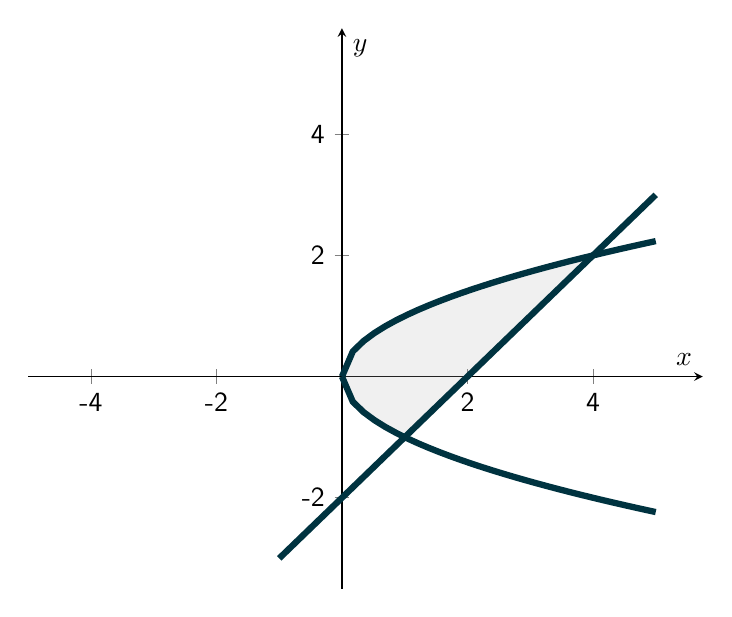
\begin{tikzpicture}[scale=1.25]
            \begin{axis}[
            axis lines = middle, very thick,
            xlabel = {$x$},
            ylabel = {$y$},
            xmin=-5, xmax=5.75,
            ymin=-3.5, ymax=5.75,
            xtick={-4,-2,0,2,4},
            xticklabels={-4,-2,0,2,4},
            ytick={-2,0,2,4},
            yticklabels={-2,0,2,4}        
            ]
            % Curves
            \addplot [name path = A,-,domain = 0:5, line width=0.8mm,DarkBlue,samples = 30] {sqrt(x)} ;
            \addplot [name path = B,-,domain = 0:5, line width=0.8mm,DarkBlue,samples = 30] {-sqrt(x)} ;
            \addplot [name path = C, line width=0.8mm, samples=4, smooth,domain=0:5, DarkBlue] coordinates {(-1,-3)(5,3)};
            % Fill area between paths
            \addplot [black!30, opacity=0.2] fill between [of = A and B, soft clip={domain=0:1}];
            \addplot [black!30, opacity=0.2] fill between [of = A and C, soft clip={domain=1:4}];
            \end{axis}
        \end{tikzpicture}    
    \end{center}   
        
    Thus
    \begin{align}
        \bar y &= \frac{M_x}M = \frac1M \int_{-1}^{2}\int_{y^2}^{y+2} 12y \, dx \, dy
    \end{align} 
    Thus
    \begin{align}
        a &= -1 \\
        b &= 2 \\
        c&= y^2 \\
        d&= y+2 \\
        f(x,y) &= \delta y = 12y
    \end{align}
    }
   \else

   \fi
    
\fi

\ifnum \Version=7
% SHORT SPHERICAL AND CYLINDRICAL EXERCISE
\part Point $P$ has rectangular (Cartesian) coordinates $(x,y,z) = (-6,0,8)$ in $\mathbb R^3$. In cylindrical coordinates, the point is $(r,\theta,z)$, and in spherical coordinates the point is $(\rho, \phi, \theta)$. Where $r=\framebox{\strut\hspace{1cm}}$, $\theta=\framebox{\strut\hspace{2cm}}$, $z=\framebox{\strut\hspace{1cm}}$, $\rho=\framebox{\strut\hspace{2cm}}$, and $\phi=\framebox{\strut\hspace{3cm}}$. 

    \ifnum \Solutions=1 {\color{DarkBlue} \textit{Solutions:} To convert to cylindrical we can use the equation $r^2 = x^2 + y^2$. 
    \begin{align}
        r^2 &= x^2 + y^2 = (-6)^2 + 0^2 = 36 \ \Rightarrow \ r = 6
    \end{align}
    To determine $\theta$ we can use $\tan\theta = y/x$. 
    \begin{align}
        \tan \theta &= \frac{y}{x} = \frac{0}{-6} = 0  \\
        \theta &= \arctan 0 
    \end{align} 
    The point in cylindrical is: 
    \begin{align}
        (r,\theta,z) &= (6,\pi,8) \\
        r &= 6 \\
        \theta &= \pi \\
        z &= 8
    \end{align}
    In spherical, we can start by obtaining $\rho$. 
    \begin{align}
        \rho^2 &= x^2+y^2+z^2\\
        \rho^2 &= (-6)^2 + 0^2 + 8^2 = 36+64 = 100 \\
        \rho &= 10
    \end{align}
    To obtain $\phi$ we can use the equation that relates $x$ to spherical. Using the expression for $x$, and the values that we already have for $x$, $\rho$ and $\theta$:
    \begin{align}
        x &= \rho \sin\phi \cos\theta \\
        -6 &= 10\sin\phi \cos(\pi) \\
        \sin\phi &= \frac{-6}{10 \cos(\pi)}  = \frac{6}{10}\\
        \phi &= \arcsin (6/10)
    \end{align}
    Our coordinates in spherical are
    \begin{align}
        \rho &= 10\\
        \phi &= \arcsin (6/10)\\
        \theta &= \pi
    \end{align}
    Note the following.
    \begin{itemize}
        \item We can, for this exercise, leave un-evaluated trig functions in the answer, because the question didn't specify that you should simplify your answer as much as possible. So it would be ok to leave your answer for $\theta$ as $\arctan 0$ or $\tan^{-1} 0$. 
        \item Our particular textbook uses the convention $(\rho, \phi, \theta)$, not $(\rho, \theta,\phi)$.
    \end{itemize}
    } 
    \else
      
    \fi
    
\fi





\ifnum \Version=8
% SHORT SPHERICAL AND CYLINDRICAL EXERCISE
\part Point $P$ has rectangular (Cartesian) coordinates $(x,y,z) = (4,4,7)$ in $\mathbb R^3$. In cylindrical coordinates, the point is $(r,\theta,z)$, and in spherical coordinates the point is $(\rho, \phi, \theta)$. Where $r=\framebox{\strut\hspace{1cm}}$, $\theta=\framebox{\strut\hspace{2cm}}$, $z=\framebox{\strut\hspace{1cm}}$, $\rho=\framebox{\strut\hspace{2cm}}$, and $\phi=\framebox{\strut\hspace{3cm}}$. 

    \ifnum \Solutions=1 {\color{DarkBlue} \textit{Solutions:} To convert to cylindrical we can use the equation $r^2 = x^2 + y^2$. 
    \begin{align}
        r^2 &= x^2 + y^2 = (4)^2 + 4^2 = 32 \ \Rightarrow \ r = \sqrt{32} = 4\sqrt2
    \end{align}
    It isn't necesssary to simplify to $4\sqrt2$. Then to determine $\theta$ we can use $\tan\theta = y/x$. 
    \begin{align}
        \tan \theta &= \frac{y}{x} = \frac{4}{4} = 1  \\
        \theta &= \arctan \pi/4
    \end{align} 
    The point in cylindrical is: 
    \begin{align}
        (r,\theta,z) &= (4\sqrt2,\pi/4,7) \\
        r &= 4\sqrt2 \\
        \theta &= \pi/4 \\
        z &= 7
    \end{align}
    In spherical, we can start by obtaining $\rho$. 
    \begin{align}
        \rho^2 &= x^2+y^2+z^2\\
        \rho^2 &= (4)^2 + 4^2 + 7^2 = 16+16+49 = 32+49 = 81 \\
        \rho &= 9
    \end{align}
    To obtain $\phi$ we can use the equation that relates $x$ to spherical. Using the expression for $x$, and the values that we already have for $x$, $\rho$ and $\theta$:
    \begin{align}
        x &= \rho \sin\phi \cos\theta \\
        4 &= 9\sin\phi \cos(\pi/4) \\
        \sin\phi &= \frac{4}{9 \cos(\pi/4)}  = \frac{4\sqrt2}{9}\\
        \phi &= \arcsin \left(\frac{4\sqrt2}{9}\right)
    \end{align}
    Note for $\phi$ we can also use:
    \begin{align}
        y &= \rho \sin\phi \sin\theta \\
        4 &= 9\sin\phi \sin(\pi/4) \\
        \sin\phi &= \frac{4}{9 \sin(\pi/4)}  = \frac{4\sqrt2}{9}\\
        \phi &= \arcsin \left(\frac{4\sqrt2}{9}\right)
    \end{align}    
    And we can also use:
    \begin{align}
        z &= \rho \cos\phi  \\
        7 &= 9\cos\phi  \\
        \sin\phi &= \frac{4}{9 \sin(\pi/4)}  = \frac{4\sqrt2}{9}\\
        \phi &= \arccos \left(\frac{7}{9}\right)
    \end{align}      
    Our coordinates in spherical are
    \begin{align}
        \rho &= 9\\
        \phi &= \arcsin \left(\frac{4\sqrt2}{9}\right), \ \textbf{or} \ \phi = \arccos(7/9)\\
        \theta &= \pi/4
    \end{align}
    Note the following.
    \begin{itemize}
        \item We can, for this exercise, leave un-evaluated trig functions in the answer, because the question didn't specify that you should simplify your answer as much as possible. So it would be ok to leave your answer for $\theta$ as $\arctan 1$ or $\tan^{-1} 1$. 
        \item Our particular textbook uses the convention $(\rho, \phi, \theta)$, not $(\rho, \theta,\phi)$.
    \end{itemize}
    } 
    \else
      
    \fi
    
\fi





% 15.6
% CENTROID Y-COORDINATE PARABOLA AND LINE
\ifnum \Version=9
    \part A thin plate with density $\delta=12$ is bounded in the $xy-$plane by $y=3-x^2$ and $y=1-x$. The plate has mass $M$. The $y-$coordinate of the centroid is $\bar y = M_x/M$, where $\displaystyle M_x = \int_A^B \int_C^D f(x,y) \, dy \, dx$,  and $A=\framebox{\strut\hspace{1cm}}$, $B=\framebox{\strut\hspace{1cm}}$, $C=\framebox{\strut\hspace{3cm}}$, $D=\framebox{\strut\hspace{3cm}}$, and $f(x,y) = \framebox{\strut\hspace{3cm}}$. 
    
    \ifnum \Solutions=1 
    {\color{DarkBlue}
    The region is bounded by 
    $$1-x \le y \le 3-x^2$$
    The given curves intersect when 
    \begin{align}
        1-x &= 3-x^2\\
        0 &= x^2-x-2 \\
        &= (x-2)(x+1)
    \end{align}
    The curves intersect at $x=-1,2$. Using $y=1-x$, the intersection points are $(-1,2)$ and $(2,-1)$. The region is shown below. 
    \begin{center}  
        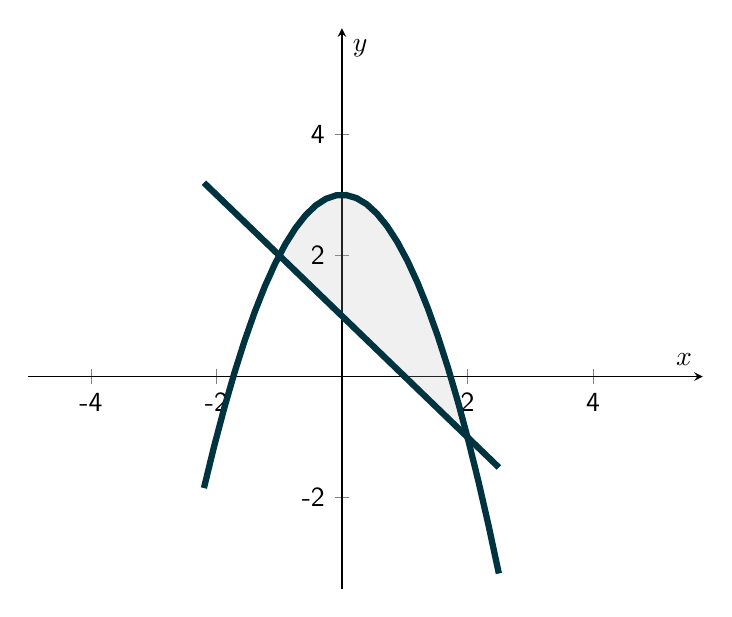
\begin{tikzpicture}[scale=1.25]
            \begin{axis}[
            axis lines = middle, very thick,
            xlabel = {$x$},
            ylabel = {$y$},
            xmin=-5, xmax=5.75,
            ymin=-3.5, ymax=5.75,
            xtick={-4,-2,0,2,4},
            xticklabels={-4,-2,0,2,4},
            ytick={-2,0,2,4},
            yticklabels={-2,0,2,4}        
            ]
            % Curves
            \addplot [name path = A,-,domain = -2.2:2.5, line width=0.8mm,DarkBlue,samples = 30] {3-x^2} ;
            \addplot [name path = C,-,domain = -2.2:2.5, line width=0.8mm,DarkBlue,samples = 4] {1-x} ;
            % Fill area between paths
            \addplot [black!30, opacity=0.2] fill between [of = A and C, soft clip={domain=-1:2}];
            \end{axis}
        \end{tikzpicture}    
    \end{center}   
        
    Thus
    \begin{align}
        \bar y &= \frac{M_x}M = \frac1M \int_{-1}^{2}\int_{1-x}^{3-x^2} 12y \, dy \, dx
    \end{align} 
    Thus
    \begin{align}
        A &= -1 \\
        B &= 2 \\
        C&= 1-x \\
        D&= 3-x^2 \\
        f(x,y) &= \delta y = 12y
    \end{align}
    }
   \else

   \fi
    
\fi
   
    % 13.3 and 13.4
% unit tangent vectors
% arc length
% curvature
% osculating circle
% unit normal

\ifnum \Version=1

\part The unit tangent vector for a curve $\mathbf r(t)$ is $\mathbf T(t) = \langle 0, \cos t, \sin t \rangle$. The unit normal vector is $\mathbf  N = \langle f(t), g(t), g(t) \rangle$, where $f(t) = \framebox{\strut\hspace{2cm}}$, $g(t) = \framebox{\strut\hspace{2cm}}$, $h(t) =\framebox{\strut\hspace{2cm}}$. 

\ifnum \Solutions=1 {\color{DarkBlue} \textit{Answer:} \textit{Solutions:} The normal vector is

\begin{align}
    \mathbf N &= \frac{d\mathbf T/dt}{|d\mathbf T/dt|} 
\end{align}
And
\begin{align}
    \mathbf T'(t) &= \langle 0,-\sin t, \cos t \rangle \\
    |\mathbf T'(t) | &= \sqrt{ 0 +(-\sin t)^2 + (\cos t)^2} =1\\
    \mathbf N &= \frac{d\mathbf T/dt}{|d\mathbf T/dt|} = \langle 0, - \sin(t),  \cos(t) \rangle
\end{align}
} 
\else
\fi        
\fi

\ifnum \Version=2

\part The velocity vector of an object moving on the curve $\mathbf r(t)$ is $\mathbf v(t) = \langle 4\cos (2t), 4\sin (2t) , 3 \rangle$ for $t>0$. The speed of the object for $t>0$ is $s(t) = |\mathbf v | = \framebox{\strut\hspace{1cm}}$. The unit tangent vector for $t>0$ is $\mathbf T = \langle f(t), g(t) , h(t) \rangle$, where $f(t) = \framebox{\strut\hspace{1.5cm}}$, $g(t) = \framebox{\strut\hspace{1.5cm}}$, $h = \framebox{\strut\hspace{1cm}}$. The curvature is $\kappa = \framebox{\strut\hspace{1cm}}$. 

\ifnum \Solutions=1 {\color{DarkBlue} \textit{Answer:} \textit{Solutions:} The speed is the magnitude of the given velocity vector and is
\begin{align}
    s &= |\mathbf v | =  \sqrt{(4\cos2t)^2 + (4\sin2t)^2 + 3^2 } = \sqrt{4^2 (\cos ^2 2 t + \sin^2 2t) + 3^2} = \sqrt{16 + 9} = 5
\end{align}
The unit tangent vector is 
\begin{align}
    \mathbf T &= \frac{\mathbf v}{|\mathbf v|} = \langle \frac{4}{5}\cos(2 t) , \frac 45 \sin (2t), \frac35 \rangle
\end{align}
For curvature we also need
\begin{align}
    \frac{d\mathbf T}{dt } &= \langle -\frac85 \sin 2t, \frac85 \cos 2t,0 \rangle \\
    \left | \frac{d\mathbf T}{dt } \right| &= \sqrt{ \left(-\frac85\sin 2t\right)^2 +   \left(\frac85 \cos 2 t\right)^2 } = \frac85
\end{align}
The curvature is
\begin{align}
    \kappa = \frac{1}{|\mathbf v |}\left| \frac{d\mathbf T}{dt}\right| = \frac{1}{5} \cdot \frac{8}{5} = \frac{8}{25}
\end{align}
} 
\else
\fi        
\fi


\ifnum \Version=3

\part A plane curve $\mathbf r(t)$ has curvature $\kappa = \frac{1}{8}$ at $\mathbf r(t_0) = \langle 15, 2 \rangle$, and the unit normal vector at $t=t_0$ is $\mathbf  N = \mathbf j = \langle 0, 1 \rangle$. The equation of the osculating circle at $t=t_0$ is \framebox{\strut\hspace{3.5cm}}.

\ifnum \Solutions=1 {\color{DarkBlue} \textit{Answer:} \textit{Solutions:} Recall that The circle of curvature, or osculating circle, at a point $P$ on a plane curve where $\kappa \ne 0$ is the circle in the plane of the curve that

\begin{enumerate}
    \item is tangent to the curve at P (has the same tangent line the curve has)
    \item has the same curvature the curve has at P
    \item lies toward the concave or inner side of the curve
\end{enumerate}
The \textbf{radius of curvature} of the curve at P is the radius of the circle of curvature, which is $\frac{1}{\kappa}$. So to obtain the radius, we calculate $\kappa$ and take the reciprocal. The \textbf{center} of the osculating circle of the curve at P lies on the inner side of the curve, and the unit normal points in the direction of the inner side of the planar curve. 

So for this problem we have a circle with radius $1/\kappa = 8$, and whose centre is 8 units away from the point $(15,2)$ in the direction of $\mathbf N$. The circle has equation
$$(x-15)^2 + (y-10)^2 = 8^2$$
} 
\else
  
\fi        
\fi




\ifnum \Version=4

\part The velocity vector for an object moving on the curve $\mathbf r(t)$ is $\mathbf v(t) = \langle t\cos t, t\sin t \rangle$. The speed of the object for $t>0$ is $s(t) = \framebox{\strut\hspace{1cm}}$. The unit tangent vector for $t>0$ is $\mathbf T = \langle f(t), g(t) \rangle$, where $f(t) = \framebox{\strut\hspace{2cm}}$, $g(t) = \framebox{\strut\hspace{2cm}}$. 

\ifnum \Solutions=1 {\color{DarkBlue} \textit{Answer:} \textit{Solutions:} The speed is the magnitude of the velocity vector and is
\begin{align}
    s &= |\mathbf v | = \sqrt{(t\cos t)^2 + (t\sin t)^2 } = \sqrt{t^2 (\cos ^2 t + \sin^2 t)} = |t|
\end{align}
But we are told that $t>0$ so we can use $|t| = t$. The unit tangent vector is 
\begin{align}
    \mathbf T &= \frac{\mathbf v}{|\mathbf v|} = \langle \cos t, \sin t \rangle
\end{align}
} 
\else
\fi        
\fi

\ifnum \Version=5

\part A plane curve $\mathbf r(t)$ has curvature $\kappa = \frac{1}{4}$ at the point $\mathbf r(t_0) = 3\mathbf i + 5\mathbf j$, and the unit normal vector at $t_0$ is $\mathbf  N = \mathbf i = \langle1,0\rangle$. The equation of the osculating circle at $t=t_0$ is \framebox{\strut\hspace{3.5cm}}.

\ifnum \Solutions=1 {\color{DarkBlue} \textit{Answer:} \textit{Solutions:} Recall that The circle of curvature, or osculating circle, at a point $P$ on a plane curve where $\kappa \ne 0$ is the circle in the plane of the curve that

\begin{enumerate}
    \item is tangent to the curve at P (has the same tangent line the curve has)
    \item has the same curvature the curve has at P
    \item lies toward the concave or inner side of the curve
\end{enumerate}
The \textbf{radius of curvature} of the curve at P is the radius of the circle of curvature, which is $\frac{1}{\kappa}$. So to obtain the radius, we calculate $\kappa$ and take the reciprocal. The \textbf{center} of the osculating circle of the curve at P lies on the inner side of the curve, and the unit normal points in the direction of the inner side of the planar curve. 

So for this problem we have a circle with radius $1/\kappa = 4$, and whose centre is 4 units away from the point $(3,5)$ in the direction of $\mathbf N$. The circle has equation
$$(x-7)^2 + (y-5)^2 = 4^2$$
} 
\else
  
\fi        
\fi


\ifnum \Version=6

\part The velocity vector for an object moving on the curve $\mathbf r(t)$ is $\mathbf v(t) = \langle 4t\cos t, 4t\sin t \rangle$ for $t>0$. The speed of the object for $t>0$ is $s(t)  = |\mathbf v | = \framebox{\strut\hspace{1cm}}$. The unit tangent vector for $t>0$ is $\mathbf T = \langle f(t), g(t) \rangle$, where $f(t) = \framebox{\strut\hspace{1.5cm}}$, $g(t) = \framebox{\strut\hspace{1.5cm}}$. The curvature is $\kappa = \framebox{\strut\hspace{1cm}}$. 

\ifnum \Solutions=1 {\color{DarkBlue} \textit{Answer:} \textit{Solutions:} The speed is the magnitude of the given velocity vector and is
\begin{align}
    s &= |\mathbf v | =  \sqrt{(4t\cos t)^2 + (4t\sin t)^2 } = \sqrt{4^2t^2 (\cos ^2 t + \sin^2 t)} = 4|t|
\end{align}
But we are told that $t>0$ so we can assume $|t| = t$. The unit tangent vector is 
\begin{align}
    \mathbf T &= \frac{\mathbf v}{|\mathbf v|} = \langle \cos t, \sin t \rangle
\end{align}
We need
\begin{align}
    \frac{d\mathbf T}{dt } &= \langle -\sin t, \cos t \rangle \\
    \left | \frac{d\mathbf T}{dt } \right| &= \sqrt{ (-\sin t)^2 +   \cos^2 t } = 1
\end{align}
The curvature is
\begin{align}
    \kappa = \frac{1}{|\mathbf v |}\left| \frac{d\mathbf T}{dt}\right| = \frac{1}{4t} 
\end{align}
} 
\else
\fi        
\fi



\ifnum \Version=7

\part The velocity vector of an object moving on the curve $\mathbf r(t)$ is $\mathbf v(t) = \langle 3\cos (2t), 3\sin (2t) \rangle$ for $t>0$. The speed of the object for $t>0$ is $s(t) = |\mathbf v | = \framebox{\strut\hspace{1.5cm}}$. The unit tangent vector for $t>0$ is $\mathbf T = \langle f(t), g(t)  \rangle$, where $f(t) = \framebox{\strut\hspace{2cm}}$, and $g(t) = \framebox{\strut\hspace{2cm}}$.  The curvature for $t>0$ is \framebox{\strut\hspace{1.5cm}}. 

\ifnum \Solutions=1 {\color{DarkBlue} \textit{Answer:} \textit{Solutions:} The speed is the magnitude of the given velocity vector and is
\begin{align}
    s &= |\mathbf v | =  \sqrt{(3\cos t)^2 + (3\sin t)^2  } = \sqrt{3^2 (\cos ^2 t + \sin^2 t) + 3^2} = \sqrt{ 9} = 3
\end{align}
The unit tangent vector is 
\begin{align}
    \mathbf T &= \frac{\mathbf v}{|\mathbf v|} 
    = \langle \frac{3}{3}\cos(2 t) , \frac 33 \sin (2t) \rangle 
    = \langle \cos(2 t) ,  \sin (2t) \rangle
\end{align}
For curvature we also need
\begin{align}
    \frac{d\mathbf T}{dt } &= \langle -2 \sin 2t, 2 \cos 2t\rangle \\
    \left | \frac{d\mathbf T}{dt } \right| &= \sqrt{ \left(-2\sin 2t\right)^2 +   \left(2 \cos 2 t\right)^2 } = 2
\end{align}
The curvature is
\begin{align}
    \kappa = \frac{1}{|\mathbf v |}\left| \frac{d\mathbf T}{dt}\right| = \frac{1}{3} \cdot 2 = \frac{2}{3}
\end{align}
} 
\else
\fi        
\fi


\ifnum \Version=8

\part A plane curve $\mathbf r(t)$ has curvature $\kappa = \frac{1}{4}$ at $\mathbf r(t_0) = \langle 5, 3 \rangle$, and the unit normal vector at $t=t_0$ is $\mathbf  N = \mathbf j = \langle 0, 1 \rangle$. The equation of the osculating circle at $t=t_0$ is \framebox{\strut\hspace{3.5cm}}.

\ifnum \Solutions=1 {\color{DarkBlue} \textit{Answer:} \textit{Solutions:} Recall that The circle of curvature, or osculating circle, at a point $P$ on a plane curve where $\kappa \ne 0$ is the circle in the plane of the curve that

\begin{enumerate}
    \item is tangent to the curve at P (has the same tangent line the curve has)
    \item has the same curvature the curve has at P
    \item lies toward the concave or inner side of the curve
\end{enumerate}
The \textbf{radius of curvature} of the curve at P is the radius of the circle of curvature, which is $\frac{1}{\kappa}$. So to obtain the radius, we calculate $\kappa$ and take the reciprocal. The \textbf{center} of the osculating circle of the curve at P lies on the inner side of the curve, and the unit normal points in the direction of the inner side of the planar curve. 

So for this problem we have a circle with radius $1/\kappa = 4$, and whose centre is 4 units away from the point $(5,3)$ in the direction of $\mathbf N$. The circle has equation
$$(x-5)^2 + (y-7)^2 = 4^2$$
} 
\else
  
\fi        
\fi






\ifnum \Version=9

\part The velocity vector of an object moving on the curve $\mathbf r(t)$ is $\mathbf v(t) = \langle t, 3 \rangle$ for $t>0$. The speed of the object at $t=2$ is $s(2) = |\mathbf v(2) | = \framebox{\strut\hspace{1.75cm}}$. The unit tangent vector at $t=2$ is $\mathbf T(2) = \langle c_1 ,c_2  \rangle$, where $c_1 = \framebox{\strut\hspace{1.75cm}}$, $c_2 = \framebox{\strut\hspace{1.75cm}}$. The curvature is $\framebox{\strut\hspace{1.75cm}}$. 

\ifnum \Solutions=1 {\color{DarkBlue} \textit{Answer:} \textit{Solutions:} The speed is the magnitude of the given velocity vector and is
\begin{align}
    s &= |\mathbf v | =  \sqrt{( t)^2 + (3)^2  } = \sqrt{t^2+9}\\
    s(2) &= \sqrt{2^2+9} = \sqrt{13}
\end{align}
We also need the unit tangent vector at $t=2$. 
\begin{align}
    \mathbf T (t) &= \frac{\mathbf v}{|\mathbf v|} = \frac{t\mathbf i + 3\mathbf j}{\sqrt{t^2+9}} \\
    \mathbf T (2) &= \frac{2\mathbf i + 3\mathbf j}{\sqrt{2^2+9}}  
    = \langle \frac{2}{\sqrt{13}} , \frac {3}{\sqrt{13}}  \rangle \\
    c_1 &= \frac{2}{\sqrt{13}}\\
    c_2 &= \frac{3}{\sqrt{13}}
\end{align}
The curvature is zero because the motion is along a straight line. 
\begin{align}
    \kappa = 0
\end{align}
} 
\else
\fi        
\fi

\ifnum \Version=10

\part A plane curve $\mathbf r(t)$ has curvature $\kappa = \frac{1}{10}$ at $\mathbf r(t_0) = \langle 5, 0 \rangle$, and the unit normal vector at $t=t_0$ is $\mathbf  N = \mathbf j = \langle 0, 1 \rangle$. The equation of the osculating circle at $t=t_0$ is \framebox{\strut\hspace{3.5cm}}.

\ifnum \Solutions=1 {\color{DarkBlue} \textit{Answer:} \textit{Solutions:} Recall that The circle of curvature, or osculating circle, at a point $P$ on a plane curve where $\kappa \ne 0$ is the circle in the plane of the curve that

\begin{enumerate}
    \item is tangent to the curve at P (has the same tangent line the curve has)
    \item has the same curvature the curve has at P
    \item lies toward the concave or inner side of the curve
\end{enumerate}
The \textbf{radius of curvature} of the curve at P is the radius of the circle of curvature, which is $\frac{1}{\kappa}$. So to obtain the radius, we calculate $\kappa$ and take the reciprocal. The \textbf{center} of the osculating circle of the curve at P lies on the inner side of the curve, and the unit normal points in the direction of the inner side of the planar curve. 

So for this problem we have a circle with radius $1/\kappa = 10$, and whose centre is 10 units away from the point $(5,0)$ in the direction of $\mathbf N$. The circle has equation
$$(x-5)^2 + (y-10)^2 = 10^2$$
} 
\else
  
\fi        
\fi
   
\end{parts}

\newpage \question[0.25] \ID
% CHANGE OF VARIABLE (15.8)
% OR APPLICATION (15.6)
% OR TRIPLE CARTESIAN (15.5) 

\ifnum \Version=1
% CENTROID
% BASED ON THOMAS EXERCISES, 15.6 #1
% SUFFICIENT FOR A PRACTICE EXAM
\question[6] A thin plate of density $\delta(x,y) = 12x$ is bounded by the lines $x = 0, y = x$, and the parabola $y = x^2-6$ in the first quadrant. 
\begin{parts} 
    \part Determine the mass of the plate, $M$. Please show your work. 
    \ifnum \Solutions=1 
    {\color{DarkBlue} \textit{Solutions:}
    Curves intersect when $$x = x^2-6 \quad \Rightarrow \quad 0 = x^2 - x - 6 = (x-3)(x+2)$$
    Or $x=3, -2$. We can ignore $x=-2$ because the region is the first quadrant. Curves intersect at the point $(3,3)$, and 
    \begin{align}
        0 \le y \le 3, \quad y \le x \le \sqrt{y+6}
    \end{align}
    The mass is
    \begin{align}
        M &= \int_0^3 \int_y^{\sqrt{y+6}} \delta \, dx \, dy \\
        &= \int_0^3 \int_y^{\sqrt{y+6}} 12x \, dx \, dy \\
        &= \int_0^3  \left. 6x^2 \right|_{x=y}^{x=\sqrt{y+6}} \, dy \\
        &= \int_0^3 6(y + 6 - y^2) \, dy \\
        &= \int_0^3 6y + 36 - 6y^2 \, dy \\
        &= \left. (3y^2 + 36y - 2y^3 ) \right|_0^3 \, dy \\
        &= 27 + 108 - 54 \\
        &= 81
    \end{align}
    }
    \else 
    \vspace{16cm}
    \fi
    \part Use your results from the previous part to set up an integral that can be used to determine the $x-$coordinate of the center of mass of the plate. You do not need to evaluate your integral. 
    \ifnum \Solutions=1 {\color{DarkBlue} \textit{Solutions:} the $x-$coordinate of the center of mass, $\bar x$, is
    \begin{align}
    \bar x &= \frac{M_y}{M} = \frac{1}{81} \int_0^3 \int_y^{\sqrt{y+6}} 12x^2 \, dx \, dy 
    \end{align}
    } 
    \else
      
    \fi
    \end{parts} 
\fi
    





\ifnum \Version=2
% LONGISH CHANGE OF VARIABLE
% VERBATUM FROM SPRING 2022 QUIZ
% hand written solution only
% SUFFICIENT FOR A PRACTICE EXAM
\question[6] Consider the double integral

$$I=\iint_R \frac{x+2y}{2y-x} dA$$

where $R$ is the parallelogram with vertices $(-3,1), (-1,0), (-1,2), (1,1)$. Our goal is to determine the area of the parallelogram using the transform below. 
$$u=x+2y, \qquad v = -x +2y$$ 
Please show your work for the following. 
\begin{parts} 
    \part Use the given transform to calculate the Jacobian of the transform, $J = \partial x(u,v)/\partial y(u,v)$. 
    \ifnum \Solutions=1 
    \else 
    \vspace{8 cm}
    \fi
    \part Use your results from Part (a) and the given transform to transform the double integral. You do not need to evaluate your integral. 
\end{parts} 

\ifnum \Solutions=1 {\color{DarkBlue} \textit{Solutions:} the integral after the transform is $$\displaystyle \frac14 \int_1^5\int_{-1}^3 \frac uv \, du \, dv$$
A screen capture of a hand-written solution from a previous offer of MATH 2551 is below. 
    \begin{figure}[h]
    \centering
    \includegraphics[width=16cm]{202302/Exam3/Images/ImgE3.OR.06.png}
    \end{figure}  
    
    } 
   \else
      
   \fi
    
\fi

\ifnum \Version=3
% CENTROID
% BASED ON THOMAS EXERCISES, 15.6 #1
% SUFFICIENT FOR A PRACTICE EXAM
\question[6] A thin plate with density $\delta(x,y) = 24y$ is bounded by the lines $x = 0, x=2y$, and the parabola $x=y^2$ in the first quadrant. 
\begin{parts} 
    \part Determine the mass of the plate, $M$. Please show your work. 
    
    \ifnum \Solutions=1 
    {\color{DarkBlue} \textit{Solutions:}
    Curves intersect when $$2y = y^2 \quad \Rightarrow \quad 0 = y^2-2y = y(y-2)$$
    Or $y=0,2$. Curves intersect at the points $(0,0)$, $(4,2)$. 
    The mass is
    \begin{align}
        M = \int_0^4 \int_{x/2}^{\sqrt{x}} \delta \, dy \, dx 
        &= \int_0^4 \int_{x/2}^{\sqrt{x}} 24y \, dy \, dx \\
        &= \int_0^4  \left. 12y^2 \right|_{y=x/2}^{y=\sqrt{x}} \, dx \\
        &= 12 \int_0^4 (x-\frac{x^2}{4}) \, dx \\
        &= 12 \left. (\frac{x^2}{2} - \frac{x^3}{12} ) \right|_0^4 \, dy \\
        &= 12 (\frac{16}{2} - \frac{64}{12}) \\
        &= 96 - 64\\
        &= 32
    \end{align}
    \textbf{An Alternate Solution}\\
    Another way to approach this problem is to use the integration order $dx\,dy$. In this case the double integral becomes
    \begin{align}
        M = \int_0^2 \int_{y^2}^{2y} \delta \, dx \, dy
        &= \int_0^2 \int_{y^2}^{2y} 24y \, dx \, dy \\
        &= 24\int_0^2  \left. yx \right|_{x=y^2}^{x=2y} \, dy \\
        &= 24 \int_0^2 (2y^2 - y^3) \, dy \\
        &= 24 \left. (\frac{2y^3}{3} - \frac{y^4}{4} ) \right|_0^2 \, dy \\
        &= 24 (\frac{16}{3} - \frac{16}{4}) \\
        &= \frac{24\cdot16}{3} - 24\cdot 4 \\
        &= 8\cdot16 - 96 \\
        &= 128 - 96 \\
        &= 32
    \end{align}    
    }
    \else 
    \vspace{14cm}
    \fi
    \part Use your results from the previous part to set up an integral that can be used to determine the $x-$coordinate of the center of mass of the plate. You do not need to evaluate your integral. 
    \ifnum \Solutions=1 {\color{DarkBlue} \textit{Solutions:} the $x-$coordinate of the center of mass, $\bar x$, is
    \begin{align}
    \bar x &= \frac{M_y}{M} = \frac{1}{32} \int_0^4 \int_{x/2}^{\sqrt{x}} 24xy \, dy \, dx
    \end{align}
    \textbf{An Alternate Solution}\\    
    It is also ok to use the integration order $dx\,dy$. In this case the double integral becomes
    \begin{align}
    \bar x &= \frac{M_y}{M} = \frac{1}{32} \int_0^2 \int_{y^2}^{2y} 24xy \, dx \, dy 
    \end{align}
    } 
    \else
      
    \fi
    \end{parts} 
\fi

\ifnum \Version=4
% VERSION B
% LONG CHANGE OF VARIABLE
% BASED ON AN EXAMPLE FROM THOMAS
% SECTION 15.8 FROM THOMAS
\question[6] Consider the double integral

$$I= 9 \iint_R (y-2x)^2 \sqrt{x+y} \, dA$$

where $R$ is the region in the first quadrant bounded by the lines $x=0$, $y=0$, and $y=1-x$. Our goal is to determine the area of $R$ using the transform below. 
$$u=x+y, \qquad v = y-2x$$ 
Please show your work for the following. 
\begin{parts} 
    \part Use the given transform to calculate the Jacobian of the transform, $J = \partial x(u,v)/\partial y(u,v)$. 
    \ifnum \Solutions=1 {\color{DarkBlue} \textit{Solutions:} Solving for $x$ and $y$ using an augmented matrix,
    \begin{align}
        \begin{pmatrix} 1 & 1 & u \\-2 & 1 & v\end{pmatrix} 
        \sim \begin{pmatrix} 1 & 1 & u \\0 & 3 & 2u+v\end{pmatrix} 
        \sim \begin{pmatrix} 1 & 0 & u/3 - v/3 \\0 & 1 & 2u/3+v/3 \end{pmatrix} 
    \end{align}
    Thus
    \begin{align}
        x &= \frac13(u-v), \ y = \frac13(2u+v) \\
        J(u,v) & = \begin{vmatrix} \DXDU & \DXDV \\[8pt] \DYDU & \DYDV \end{vmatrix} = \begin{vmatrix} 1/3 & -1/3 \\ 2/3 & 1/3 \end{vmatrix} = 1/9 + 2/9 = 1/3
    \end{align}
    }
    \else 
    \vspace{8 cm}
    \fi
    \part Use the given transform and your results from Part (a) to convert the double integral into a double integral over a region in the $uv-$plane. You do not need to evaluate your integral. 
    \ifnum \Solutions=1 {\color{DarkBlue} \textit{Solutions:} Converting each of the boundaries in the $xy-$plane into the $uv-$plane we obtain
        \begin{align}
            x+y &= 1 \quad \Rightarrow \quad \frac13(u-v) + \frac13(2u+v) = 1 &&\Rightarrow \quad u = 1\\
            x&=0 \quad \Rightarrow \quad \frac13(u-v) = 0 &&\Rightarrow \quad v = u\\
            y&= 0 \quad \Rightarrow \quad \frac13(2u+v) = 0 &&\Rightarrow \quad v = -2u
        \end{align}
        The region is described by either of the following relations:
        \begin{align}
            S_1: & \quad 0 \le u \le 1, \quad -2u \le v \le u \\
            S_2: & \quad -2 \le v \le 0, \quad -v/2 \le u \le 1, \ \text{and } 0 \le v \le 1, \quad v \le u \le 1
        \end{align}
        The first set of inequalities requires only a single double integral, but it is ok to set up two double integrals. If using $S_1$, we use $dv\,du$ and obtain
        \begin{align}
            I= 9 \iint_R (y-2x)^2 \sqrt{x+y} \, dA = 9 \int_0^1 \int_{-2u}^u v^2u^{1/2} \frac13 \,dv\,du
        \end{align}
        If using $S_2$, we use $du\,dv$ and obtain
        \begin{align}
            I= 9 \iint_R (y-2x)^2 \sqrt{x+y} \, dA 
            = 9 \int_{-2}^0 \int_{-v/2}^1 v^2u^{1/2} \frac13 \,du\,dv
            + 9 \int_{0}^1 \int_{v}^1 v^2u^{1/2} \frac13 \,du\,dv
        \end{align}        
        } 
       \else
          
       \fi
    \end{parts} 

    \fi



\ifnum \Version=5
    % USE FOR VERSION B
    % LONG CYLINDRICAL WITH APPLICATION TO MASS WITH VARYING DENSITY
    % FROM 15.8
    \question[6] An object $D$ lying in the first octant is bounded below by the $xy-$plane, above by the plane $z=3+4y$, and by the cylinder $x^2+y^2 = 4$. The density of the object at any point in $D$ is equal to the distance from the point to the $z$-axis.  Please show your work for the following.
    
    \begin{parts} 
    \part Use cylindrical coordinates to calculate the total of mass of the object, $M$. Please show your work. 
    
    \ifnum \Solutions=1 {\color{DarkBlue} The object is only in the first octant so $$0 \le \theta \le \pi/2$$ Using $\delta = \sqrt{x^2+y^2} = r$, the $z-$coordinate of the center of mass is computed using 
    \begin{align}
        M &= \iiint_D  \delta \, dV \\
        &= \int_0^{\pi/2} \int_0^2 \int_0^{3+4r\sin\theta}  \delta(r,\theta) \, r\, dz\,dr\,d\theta\\
        &= \int_0^{\pi/2} \int_0^2 \int_0^{3+4r\sin\theta}   r^2 \, dz\,dr\,d\theta\\
        &= \int_0^{\pi/2} \int_0^2    r^2 \, (3+4r\sin\theta) \,dr\,d\theta \\
        &= \int_0^{\pi/2} \int_0^2     \, (3r^2+4r^3\sin\theta) \,dr\,d\theta \\
        &= \int_0^{\pi/2}  \left. \, (r^3+r^4\sin\theta) \right|_{r=0}^{r=2} d\theta \\
        &= \int_0^{\pi/2}  (8 + 16\sin\theta) d\theta \\
        &=  \left. (8\theta - 16\cos\theta) \right|_0^{\pi/2} \\
        &=  (4\pi - 0) - (0 - 16) \\
        &= 4\pi + 16
    \end{align}
    
    } 
    \else
        \vspace{14cm}
    \fi
    
    \part Use your results from the previous part to set up a triple integral in cylindrical coordinates that can be used to determine the $z-$coordinate of the center of mass of the object. You do not need to evaluate your integral. 

    \ifnum \Solutions=1 {\color{DarkBlue} \textit{Solutions:} the $z-$coordinate of the center of mass, $\bar x$, is
    \begin{align}
    \bar z &= \frac{M_{xy}}{M} = \frac{1}{16\pi+16} \int_0^{\pi/2} \int_0^2 \int_0^{3+4r\sin\theta}  z \, \delta(r,\theta) \, r\, dz\,dr\,d\theta
    \end{align}
    } 
    \else
      
    \fi
    \end{parts} 
\fi


% TRANSFORM: SOLVE FOR X & Y, BOUNDARIES, EVALUATE, TRIANGLES
% VERSION A
\ifnum \Version=6
    \question[6] Consider the transform $u=x+y$ and $v=4x+5y$, and the integral $\displaystyle I = \iint_{R}  \,dxdy$. Region $R$ is the triangle in the $xy$-plane bounded by $x+y=0$, $4x+5y=0$, $6x+7y=4$. The transform maps $R$ to region $G$ in the $uv-$plane.  Please show your work for the following.

    \begin{enumerate}
        \item[a)] Solve the system, $u=x+y$ and $v=4x+5y$, for $x$ and $y$ in terms of $u$ and $v$.
            \ifnum \Solutions=1 {\color{DarkBlue} \\[12pt] 
            \textbf{Solutions:}
            We can use the expressions for $u$ and $v$ as an augmented matrix and row reduce. 
            \begin{align}
                \begin{pmatrix} 1 & 1 & u \\ 4 & 5 & v\end{pmatrix} 
                \sim \begin{pmatrix} 1 & 1 & u \\0 & 1 & v - 4u \end{pmatrix} 
                \sim \begin{pmatrix} 1 & 0 & 5u - v \\ 0 & 1 & v - 4u \end{pmatrix} 
            \end{align}
            Thus $x = 5u - v$, and $y = v - 4u$. 
            } 
            \else 
            \vspace{5cm}
            \fi
        \item[b)] Transform the boundaries of $R$ to the $uv-$plane. In other words, determine the boundaries of $G$ in terms of $u$ and $v$. 
            \ifnum \Solutions=1 {\color{DarkBlue} \\[12pt] 
            \textbf{Solutions:} the three lines are transformed below. 
            \begin{itemize}
                \item The line $x+y=0$ becomes $u=0$. 
                \item The line $4x+5y=0$ becomes $v=0$. 
                \item The line $6x+7y=4$ is: 
                \begin{align}
                    6x+7y &=4 \\
                    6\cdot(5u-v) + 7\cdot(v-4u) &= 4\\
                    30u -28u -6v+7v &=4 \\
                    v &= 4 -2u
                \end{align}
            \end{itemize}
            } 
        \else 
        \vspace{5cm}
        \fi        
            
        \item[c)] Use the given transformation and your results from parts (a) and (b) to set up a double integral that in the $uv-$plane that is equal to $I$. Do not evaluate the integral. You also do not need to calculate the Jacobian and may use that the Jacobian of the transform is $J(u,v) = 1$.
            \ifnum \Solutions=1 {\color{DarkBlue} \\[12pt] 
            \textbf{Solutions:}
            \begin{align}
                \iint_{R} \,dx\,dy
                &= \iint_{G}  \left| J(u,v) \right| \,dv\,du 
                = \int_0^2\int_{0}^{4-2u}  \left| 1 \right| \,dv\,du 
                = \int_0^2\int_{0}^{4-2u} \,dv\,du
            \end{align}
            Note the following.
            \begin{itemize}
                \item We did not need to compute the Jacobian but it is computed as follows. 
                $$J 
                = \begin{vmatrix} x_u & x_v \\ y_u & y_v \end{vmatrix} 
                = \begin{vmatrix} 5 & -1 \\ -4 & 1\end{vmatrix} 
                = 5 - 4
                = 1$$
                \item             We did not need to evaluate the integral but if we did:
            \begin{align}
                I = \int_0^2\int_{0}^{4-2u}  \left| 1 \right| \,dv\,du
                = 1 \int_0^2 (4-2u) \,du
                =  \left. 4u - u^2 \right|_0^2 
                = 4
            \end{align}
            \item It is also ok to use the other integration order: $I = \int_0^4\int_0^{2-v/2} \, du \, dv$.
            \end{itemize}
            } 
            \else 
            \fi        
    \end{enumerate}
 
\fi 



% TRANSFORM: SOLVE FOR X & Y, BOUNDARIES, EVALUATE, PARALLELOGRAM
% VERSION A
\ifnum \Version=7
    \question[6] Consider the integral $\displaystyle I = 2\iint_{R} x-4y \,dx\,dy$, where $R$ is the parallelogram in the $xy$-plane bounded by $x-4y=2$, $x-4y=1$, $3y-x=3$, $3y-x=6$. Suppose the transform $u=x-4y$ and $v=3y-x$, maps region $R$ to region $G$ in the $uv-$plane.  Please show your work for the following.

    \begin{enumerate}
        \item[a)] Solve the system, $u=x-4y$ and $v=3y-x$, for $x$ and $y$ in terms of $u$ and $v$.
            \ifnum \Solutions=1 {\color{DarkBlue} \\[12pt] 
            \textbf{Solutions:}
            We can use the expressions for $u$ and $v$ as an augmented matrix and row reduce. 
            \begin{align}
                \begin{pmatrix} 1 & -4 & u \\ -1 & 3 & v\end{pmatrix} 
                \sim \begin{pmatrix} 1 & -4 & u \\0 & -1 & v + u\end{pmatrix} 
                \sim \begin{pmatrix} 1 & 0 & -3u-4v\\0 & 1 & -u-v\end{pmatrix} 
            \end{align}
            Thus
            \begin{align}
                x &=  -3u-4v\\
                y &= -u-v
            \end{align}

            } 
            \else 
            \vspace{5cm}
            \fi
        \item[b)] Transform the boundaries of $R$ to the $uv-$plane. In other words, determine the boundaries of $G$ in terms of $u$ and $v$. 
            \ifnum \Solutions=1 {\color{DarkBlue} \\[12pt] 
            \textbf{Solutions:} the four lines are transformed below. 
            \begin{itemize}
                \item The line $x-4y=2$ becomes $u=2$. 
                \item The line $x-4y=1$ becomes $u=1$. 
                \item The line $3y-x=3$ becomes $v=3$. 
                \item The line $3y-x=6$ becomes $v=6$. 
            \end{itemize}
            } 
        \else 
        \vspace{5cm}
        \fi        
            
        \item[c)] Use the given transformation and your results from parts (a) and (b) to set up a double integral that in the $uv-$plane that is equal to $I$. Do not evaluate the integral. You also do not need to calculate the Jacobian and may use that the Jacobian of the transform is  $J(u,v) = -1$. 
            \ifnum \Solutions=1 {\color{DarkBlue} \\[12pt] 
            \textbf{Solutions:}
            \begin{align}
                \iint_{R} 2x-8y \,dx\,dy
                = \iint_{G} 2u \left| J(u,v) \right| \,du\,dv
                = \int_3^6\int_{1}^2 2u \left| -1 \right| \,du\,dv
                = \int_3^6\int_{1}^2 2u \,du\,dv
            \end{align}
            Note the following.
            \begin{itemize}
                \item We did not need to evaluate the integral, but if we did: 
                \begin{align}
                \iint_{R} 2x-8y \,dx\,dy
                &= \iint_{G} 2u \left| J(u,v) \right| \,du\,dv\\
                &= \int_3^6\int_{1}^2 2u \left| -1 \right| \,du\,dv\\
                &= \int_3^6\left. u^2 \right|_{1}^2 \,dv\\
                &= \int_3^6 3 \,dv\\
                &= 3 \cdot(6 -3) \\
                &= 9
            \end{align}
            \end{itemize}
            } 
            \else 
            \fi        
    \end{enumerate}
 
\fi 




% TRANSFORM: SOLVE FOR X & Y, BOUNDARIES, EVALUATE
% VERSION B
\ifnum \Version=8
    \question[6] Consider the transform $u=x-y$ and $v=4y-2x$, and the integral $\displaystyle I = \iint_{R} \,dxdy$, where $R$ denotes the triangle in the $xy$-plane bounded by $x-y=2$, $4y-2x=0$, $3y=2x$. The transform maps region $R$ to region $G$ in the $uv-$plane.  Please show your work for the following.

    \begin{enumerate}
        \item[a)] Solve the system, $u=x-y$ and $v=4y-2x$, for $x$ and $y$ in terms of $u$ and $v$.
            \ifnum \Solutions=1 {\color{DarkBlue} \\[12pt] 
            \textbf{Solutions:}
            We can use the expressions for $u$ and $v$ as an augmented matrix and row reduce. 
            \begin{align}
                \begin{pmatrix} 1 & -1 & u \\ -2 & 4 & v\end{pmatrix} 
                \sim \begin{pmatrix} 1 & -1 & u \\0 & 2 & v + 2u\end{pmatrix} 
                \sim \begin{pmatrix} 1 & -1 & u\\0 & 1 & u+v/2\end{pmatrix} 
                \sim \begin{pmatrix} 1 & 0 & 2u+v/2\\0 & 1 & u+v/2\end{pmatrix} 
            \end{align}
            Thus $x = 2u+v/2$, and $y = u + \frac{v}{2}$. 
            } 
            \else 
            \vspace{5cm}
            \fi
        \item[b)] Transform the boundaries of $R$ to the $uv-$plane. In other words, determine the boundaries of $G$ in terms of $u$ and $v$. 
            \ifnum \Solutions=1 {\color{DarkBlue} \\[12pt] 
            \textbf{Solutions:} the three lines are transformed below. 
            \begin{itemize}
                \item The line $x-y=2$ becomes $u=2$. 
                \item The line $4x-2y=0$ becomes $v=0$. 
                \item The line $3y=2x$ is: 
                \begin{align}
                    3\cdot \left(u+\frac{v}{2}\right) &= 2\cdot \left( 2u+v/2 \right) \\
                    3u + 3v/2 &= 4u + v \\
                    v/2 &= u \\
                    v &= 2u 
                \end{align}
            \end{itemize}
            } 
        \else 
        \vspace{5cm}
        \fi        
            
        \item[c)] Use the given transformation and your results from parts (a) and (b) to set up a double integral that in the $uv-$plane that is equal to $I$. Do not evaluate the integral. You also do not need to calculate the Jacobian and may use that the Jacobian of the transform is  $J(u,v) = \frac12$. 
            \ifnum \Solutions=1 {\color{DarkBlue} \\[12pt] 
            \textbf{Solutions:} the region is
            $$G = \{ (u,v) \in \mathbb R^2 \, | \, 0\le u \le 2, \ 0 \le v \le 2u\}$$
            or we can use
            $$G = \{ (u,v) \in \mathbb R^2 \, | \, 0\le v \le 4, \ v/2 \le u \le 4\}$$ 
            We can write the double integral as:
            \begin{align}
                \iint_{R} \,dx\,dy
                = \iint_{G}  \left| J(u,v) \right| \,dv\,du 
                = \int_0^2\int_{0}^{2u}  \left| \frac12 \right| \,dv\,du
                = \frac12 \int_0^2\int_{0}^{2u} \,dv\,du
            \end{align}
            Note the following.
            \begin{itemize}
                \item We did not need to compute the Jacobian but it is computed as follows. 
                $$J = \begin{vmatrix} x_u & x_v \\ y_u & y_v \end{vmatrix} = \begin{vmatrix} 2 & 1/2 \\ 1 & 1/2\end{vmatrix} = 1 - 1/2 = \frac12$$
                \item We didn't need to evaluate the integral but if we did: 
                \begin{align}
                \iint_{R} \,dx\,dy
                    &= \iint_{G}  \left| J(u,v) \right| \,dv\,du\\
                    &= \int_0^2\int_{0}^{2u}  \left| \frac12 \right| \,dv\,du\\
                    &= \frac12 \int_0^2\left.  v \right|_{v=0}^{v=2u} \,du\\
                    &= \frac12 \int_0^2 2u \,du\\
                    &=  \int_0^2 u \,du\\
                    &= \frac12 \left. u^2\right|_0^2 \\
                    &= 2
            \end{align}                
            \end{itemize}
            } 
            \else 
            \fi        
    \end{enumerate}
 
\fi 









% TRANSFORM: SOLVE FOR X & Y, BOUNDARIES, EVALUATE
% VERSION D 
\ifnum \Version=9
    \question[6] Consider the transform $u=x+y$ and $v=3x+4y$, and the integral $\displaystyle I = \iint_{R} x+y \,dxdy$, where $R$ denotes the triangle in the $xy$-plane bounded by $x+y=0$, $3x+4y=2$, and $2x+3y=0$. The transform maps region $R$ to region $G$ in the $uv-$plane. Please show your work for the following.

    \begin{enumerate}
        \item[a)] Solve the system, $u=x+y$ and $v=3x+4y$, for $x$ and $y$ in terms of $u$ and $v$.
            \ifnum \Solutions=1 {\color{DarkBlue} \\[12pt] 
            \textbf{Solutions:}
            We can use the expressions for $u$ and $v$ as an augmented matrix and row reduce. 
            \begin{align}
                \begin{pmatrix} 1 & 1 & u \\ 3 & 4 & v\end{pmatrix} 
                \sim \begin{pmatrix} 1 & 1 & u \\0 & 1 & v - 3u \end{pmatrix} 
                \sim \begin{pmatrix} 1 & 0 & 4u - v \\ 0 & 1 & v - 3u \end{pmatrix} 
            \end{align}
            Thus $x = 4u - v$, and $y = v - 3u$. 
            } 
            \else 
            \vspace{5cm}
            \fi
        \item[b)] Transform the boundaries of $R$ to the $uv-$plane. In other words, determine the boundaries of $G$ in terms of $u$ and $v$. 
            \ifnum \Solutions=1 {\color{DarkBlue} \\[12pt] 
            \textbf{Solutions:} the three lines are transformed below. 
            \begin{itemize}
                \item The line $x+y=0$ becomes $u=0$. 
                \item The line $3x+4y=2$ becomes $v=2$. 
                \item The line $2x+3y$ is: 
                \begin{align}
                    2x+3y &=0 \\
                    2\cdot(4u-v) + 3\cdot(v-3u) &= 0\\
                    8u -9u  - 2v+3v &=0 \\
                    v &= u
                \end{align}
            \end{itemize}
            } 
        \else 
        \vspace{5cm}
        \fi        
            
        \item[c)] Use the given transformation and your results from parts (a) and (b) to set up a double integral that in the $uv-$plane that is equal to $I$. Do not evaluate the integral. You also do not need to calculate the Jacobian and may use that the Jacobian of the transform is $J(u,v) = 1$. 
            \ifnum \Solutions=1 {\color{DarkBlue} \\[12pt] 
            \textbf{Solutions:}
            \begin{align}
                \iint_{R} x+y \,dx\,dy
                &= \iint_{G} u \left| J(u,v) \right| \,dv\,du\\
                &= \int_0^2\int_{u}^{2} u \left| 1 \right| \,dv\,du\\
                &= \int_0^2\int_{u}^{2} u  \,dv\,du
            \end{align}
            Note the following.
            \begin{itemize}
                \item We could also instead use
                \begin{align}
                    \iint_{R} x+y \,dx\,dy &= \int_0^2\int_{0}^{v} u  \,du\,dv
                \end{align}
                \item We did not need to compute the Jacobian but it is computed as follows. 
                $$J 
                = \begin{vmatrix} x_u & x_v \\ y_u & y_v \end{vmatrix} 
                = \begin{vmatrix} 4 & -1 \\ -3 & 1\end{vmatrix} 
                = 4 - (-1)(-3)
                = 1$$
                \item It wasn't necessary to compute the integral but: 
                \begin{align}
                    \iint_{R} x+y \,dx\,dy
                    &= \iint_{G} u \left| J(u,v) \right| \,dv\,du\\
                    &= \int_0^2\int_{u}^{2} u \left| 1 \right| \,dv\,du\\
                    &= \int_0^2 2u - u^2 \,du\\
                    &= \left. \left( u^2 - \frac{u^3}{3} \right)\right|_0^2 \\
                    &= 4 - 8/3\\
                    &= 4/3
                \end{align}                
            \end{itemize}
            } 
            \else 
            \fi        
    \end{enumerate}
 
\fi 



\newpage \question[0.25] \ID
% SPHERICAL OR CYLINDRICAL (14.7)


\ifnum \Version=1
% READY TO BE USED FOR PRACTICE EXAM
% SPHERICAL INTEGRATION
% VERBATUM FROM SPRING 2022 QUIZ
% OK FOR A PRACTICE EXAM
% hand written solution only
\question[6] Evaluate the triple integral $I=\displaystyle \iiint_D \frac{16\, x}{\sqrt2}  \, dV$, where $D$ is the region in the first octant bounded by $x^2+y^2+z^2=1$ and the planes $y=0$ and $x=y$. Please show your work. Hint: you may need to use the identity $2\sin ^2x = 1 - \cos(2x)$. 

\ifnum \Solutions=1 {\color{DarkBlue} \textit{Solutions:} below is a screen capture of a hand-written solution from a previous offer of MATH 2551. 
    \begin{figure}[h]
    \centering
    \includegraphics[width=16cm]{202302/Exam3/Images/ImgE3.OR.05.png}
    \end{figure}  
    
    } 
   \else
      
   \fi
    
\fi

\ifnum \Version=2
% OK FOR A PRACTICE EXAM
% NOT SO SHORT CYLINDRICAL EXERCISE
% VERBATUM FROM SPRING 2022 QUIZ
% hand written solution only
\question[6] Use cylindrical coordinates to determine the volume of the region bounded above by $z = 4-3x^2-3y^2$ and bounded below by $z = \sqrt{x^2+y^2}$. Please show your work. 

\ifnum \Solutions=1 {\color{DarkBlue} \textit{Solutions:} below is a screen capture of a hand-written solution from a previous offer of MATH 2551. 
    \begin{figure}[h]
    \centering
    \includegraphics[width=11cm]{202302/Exam3/Images/ImgE3.OR1C.png}
    \end{figure}  
    
    There are other ways to set up this particular integral, but the above is sufficient. 

    } 
   \else
      
   \fi
    
\fi






\ifnum \Version=3
% USE FOR VERSION A
% LONG SPHERICAL WITH APPLICATION TO MASS WITH VARYING DENSITY
% FROM 15.8
\question[6] An object $D$ lying in the first octant is bounded by the planes $x=0, y=0, z=0$, and the sphere $x^2+y^2 + z^2 = 4$. The density of the object at any point in $D$ is equal to the distance from the point to the origin. 

\begin{parts}
    \part Use spherical coordinates to calculate the mass of the object, $M$. Please show your work. 
    
    \ifnum \Solutions=1 {\color{DarkBlue} Using $\delta = \sqrt{x^2+y^2+z^2} = \rho$, the mass is computed using 
    \begin{align}
        M &= \int_0^{\pi/2} \int_0^{\pi/2} \int_0^2 \delta \, \rho^2\sin\phi \, d\rho\,d\phi\,d\theta \\
        &= \int_0^{\pi/2} \int_0^{\pi/2} \int_0^2 \rho^3\sin\phi \, d\rho\,d\phi\,d\theta \\
        &= \int_0^{\pi/2} \int_0^{\pi/2} \left. \frac14 \rho^4\sin\phi \right|_0^2 \, d\phi\,d\theta \\
        &= 4 \int_0^{\pi/2} \int_0^{\pi/2} \sin\phi \, d\phi\,d\theta \\
        &= 4 \int_0^{\pi/2} \left. -\cos\phi \right|_0^{\pi/2} \, d\theta \\
        &= 4 \int_0^{\pi/2}  \, d\theta \\
        &= 2\pi
    \end{align}
    
    } 
   \else
      \vspace{14cm}
   \fi    

   \part Use your results from the previous part to set up an integral in spherical coordinates that can be used to determine the $x-$coordinate of the center of mass of the object. You do not need to evaluate your integral. 
    \ifnum \Solutions=1 {\color{DarkBlue} In spherical coordinates, $$x = \rho \sin\phi \cos\theta$$and the $x-$coordinate of the center of mass, $\bar x$, is
    \begin{align}
    \bar x &= \frac{M_{yz}}{M} \\ 
    &= \frac{1}{M} \int_0^{\pi/2} \int_0^{\pi/2} \int_0^2 (\rho \sin\phi \cos\theta) \, \delta \, \rho^2\sin\phi \, d\rho\,d\phi\,d\theta \\
    &= \frac{1}{M} \int_0^{\pi/2} \int_0^{\pi/2} \int_0^2 \rho^4\sin^2\phi \cos\theta \, d\rho\,d\phi\,d\theta 
    \end{align}
    } 
    \else
      
    \fi
    \end{parts} 
 
\fi








\ifnum \Version=4
% USE FOR VERSION B
% LONG CYLINDRICAL WITH APPLICATION TO MASS WITH VARYING DENSITY
% FROM 15.8
\question[6] An object $D$ lying in the first octant is bounded by the planes $x=0, y=0, z=0$, $z=3+4x$ and the cylinder $x^2+y^2 = 4$. The density of the object at a point in $D$ is equal to the distance from the point to the $z$-axis. 

    \begin{parts} 
    \part Use cylindrical coordinates to calculate the total of mass of the object, $M$. Please show your work. 


    \ifnum \Solutions=1 {\color{DarkBlue} \textit{Solutions:} using $\delta = \sqrt{x^2+y^2} = r$, the $z-$coordinate of the center of mass is computed using 
    \begin{align}
        M &= \iiint_D  \delta \, dV \\
        &= \int_0^{\pi/2} \int_0^2 \int_0^{3+4r\cos\theta}  \delta(r,\theta) \, r\, dz\,dr\,d\theta\\
        &= \int_0^{\pi/2} \int_0^2 \int_0^{3+4r\cos\theta}   r^2 \, dz\,dr\,d\theta\\
        &= \int_0^{\pi/2} \int_0^2 \int_0^{3+4r\cos\theta}   r^2 \, dz\,dr\,d\theta \\ 
        &= \int_0^{\pi/2} \int_0^2    r^2 \, (3+4r\cos\theta) \,dr\,d\theta \\
        &= \int_0^{\pi/2} \int_0^2     \, (3r^2+4r^3\cos\theta) \,dr\,d\theta \\
        &= \int_0^{\pi/2}  \left. \, (r^3+r^4\cos\theta) \right|_0^2 \, d\theta \\
        &= \int_0^{\pi/2}  (8+16\cos\theta) d\theta \\
        &=  \left. (8\theta+16\sin\theta) \right|_0^{\pi/2} \\
        &= 4\pi + 16  
    \end{align}
    
    } 
   \else
      \vspace{14cm}      
   \fi
    \part Use your results from the previous part to set up a triple integral that can be used to determine the $z-$coordinate of the center of mass of the object. You do not need to evaluate your integral. 

    \ifnum \Solutions=1 {\color{DarkBlue} \textit{Solutions:} the $z-$coordinate of the center of mass, $\bar x$, is
    \begin{align}
    \bar z &= \frac{M_{xy}}{M} \\
    &= \frac{1}{16 +4\pi} \int_0^{\pi/2} \int_0^2 \int_0^{3+4r\cos\theta}  z \, \delta(r,\theta) \, r\, dz\,dr\,d\theta
    \end{align}
    } 
    \else
      
    \fi
    \end{parts} 
    
\fi


\ifnum \Version=5
% USE FOR VERSION C
% LONG SPHERICAL WITH APPLICATION TO MASS WITH VARYING DENSITY
% FROM 15.8
\question[6] An object $D$ lies above the $xy-$plane and below the upper half of the sphere $x^2+y^2 + z^2 = 4$. The density of the object at any point in $D$ is equal to the distance from the point to the origin. 

\begin{parts}
    \part Use spherical coordinates to calculate the mass of the object, $M$. Please show your work. 
    
    \ifnum \Solutions=1 {\color{DarkBlue} Using $\delta = \sqrt{x^2+y^2+z^2} = \rho$, the mass is computed using 
    \begin{align}
        M &= \int_0^{2\pi} \int_0^{\pi/2} \int_0^2 \delta \, \rho^2\sin\phi \, d\rho\,d\phi\,d\theta \\
        &= \int_0^{2\pi} \int_0^{\pi/2} \int_0^2 \rho^3\sin\phi \, d\rho\,d\phi\,d\theta \\
        &= \int_0^{2\pi} \int_0^{\pi/2} \left. \frac14 \rho^4\sin\phi \right|_0^2 \, d\phi\,d\theta \\
        &= 4 \int_0^{2\pi} \int_0^{\pi/2} \sin\phi \, d\phi\,d\theta \\
        &= 4 \int_0^{2\pi} \left. -\cos\phi \right|_0^{\pi/2} \, d\theta \\
        &= 4 \int_0^{2\pi}  \, d\theta \\
        &= 8\pi
    \end{align}
    
    } 
   \else
      \vspace{14cm}
   \fi    

   \part Use your results from the previous part to set up an integral in spherical coordinates that can be used to determine the $x-$coordinate of the center of mass of the object. You do not need to evaluate your integral. 
   
    \ifnum \Solutions=1 {\color{DarkBlue} In spherical coordinates, $$x = \rho \sin\phi \cos\theta$$and the $x-$coordinate of the center of mass, $\bar x$, is
    \begin{align}
    \bar x &= \frac{M_{yz}}{M} \\ 
    &= \frac{1}{M} \int_0^{2\pi} \int_0^{\pi/2} \int_0^2 (\rho \sin\phi \cos\theta) \, \delta \, \rho^2\sin\phi \, d\rho\,d\phi\,d\theta \\
    &= \frac{1}{M} \int_0^{2\pi} \int_0^{\pi/2} \int_0^2 \rho^4\sin^2\phi \cos\theta \, d\rho\,d\phi\,d\theta 
    \end{align}
    } 
    \else
      
    \fi
    \end{parts} 

 \fi 




\ifnum \Version=6
% USE FOR VERSION B
% LONG CYLINDRICAL WITH APPLICATION TO MASS WITH VARYING DENSITY
% FROM 15.8
\question[6] An object $D$ lying in the first octant is bounded by the planes $y=x, y=0, z=0$, $z=9+8y$ and the cylinder $x^2+y^2 = 1$. The density of the object at any point in $D$ is equal to the distance from the given point to the $z$-axis. 

    \begin{parts} 
    \part Use cylindrical coordinates to calculate the total of mass of the object, $M$. Please show your work. 


    \ifnum \Solutions=1 {\color{DarkBlue} \textit{Solutions:} using $\delta = \sqrt{x^2+y^2} = r$, mass is computed using the following. 
    \begin{align}
        M &= \iiint_D  \delta \, dV \\
        &= \int_0^{\pi/4} \int_0^1 \int_0^{9+8r\sin\theta}  \delta(r,\theta) \, r\, dz\,dr\,d\theta\\
        &= \int_0^{\pi/4} \int_0^1 \int_0^{9+8r\sin\theta}   r^2 \, dz\,dr\,d\theta\\
        &= \int_0^{\pi/4} \int_0^1    r^2 \, (9+8r\sin\theta) \,dr\,d\theta \\
        &= \int_0^{\pi/4} \int_0^1     \, (9r^2+8r^3\sin\theta) \,dr\,d\theta \\
        &= \int_0^{\pi/4}  \left. \, (3r^3+2r^4\sin\theta) \right|_0^1 \, d\theta \\
        &= \int_0^{\pi/4}  (3+2\sin\theta) d\theta \\
        &=  \left. (3\theta-2\cos\theta) \right|_0^{\pi/4} \\
        &= 3\pi/4 - 2/\sqrt2  + 2
    \end{align}
    
    Note the following. 
    \begin{itemize}
        \item We could also write final answer as $M = 3\pi/4 + 2 - \sqrt2$. 
        \item We cannot use:
        \begin{align}
            M = \iiint_D  \delta \, dV 
        &= \int_0^{\pi/4}  \int_0^{9+8r\sin\theta} \int_0^1 r^2\, dr\,dz\,d\theta
        \end{align}
        In other words we can't switch the order of the innermost two integrals because the limits for $z$ use both $r$ and $\theta$. 
        \item A common error might be to use $0 \le \theta \le \pi/2$, which would give us the answer $$M = 3\pi/2 + 2 $$
        The above is not correct!         
        \item A common mistake might be to integrate with respect to the wrong variable. For example, doing something like: 
        \begin{align}
            \int_0^{\pi/4}  (3+2\sin\theta) d\theta 
            &=  \left. (3r+2\sin\theta) \right|_0^{\pi/4} 
        \end{align}     
        The above is not correct! 
    \end{itemize}
    } 
   \else
      \vspace{14cm}      
   \fi
    \part Use your results from the previous part to set up a triple integral that can be used to determine the $z-$coordinate of the center of mass of the object. You do not need to evaluate your integral. 

    \ifnum \Solutions=1 {\color{DarkBlue} \textit{Solutions:} the $z-$coordinate of the center of mass, $\bar z$, is
    \begin{align}
    \bar z 
    &= \frac{M_{xy}}{M} 
    = \frac{1}{M} \int_0^{\pi/4} \int_0^1 \int_0^{9+8r\sin\theta}  z \,  r^2\, dz\,dr\,d\theta
    \end{align}
    Note the following. 
    \begin{itemize}
        \item The limits of integration in part (b) should be identical to what was used in part (a). So if an error were made in the limits for part (a), then points should be deducted in part a. And if the limits in part (b) are the same as what were used in part (a) then no further point deductions are needed for the limits of integration. 
        \item It isn't necessary to re-state what $M$ is in this last part of the question, because it should have been found in part (a). 
    \end{itemize}    
    } 
    \else
      
    \fi
    \end{parts} 
    
\fi



\ifnum \Version=7
% USE FOR VERSION C
% LONG SPHERICAL WITH APPLICATION TO MASS WITH VARYING DENSITY
% FROM 15.8
\question[6] An object $D$ is in the shape of an ice cream cone, as it is bounded on top by the sphere $\rho =2$ and on the sides by the cone $\phi = \pi/4$. The density of the object at any point in $D$ is equal to the distance from the given point to the origin. 

\begin{parts}
    \part Use spherical coordinates to calculate the mass of the object, $M$. Please show your work. 
    
    \ifnum \Solutions=1 {\color{DarkBlue} Using $\delta = \sqrt{x^2+y^2+z^2} = \rho$, the mass is computed using 
    \begin{align}
        M &= \int_0^{2\pi} \int_0^{\pi/4} \int_0^2 \delta \, \rho^2\sin\phi \, d\rho\,d\phi\,d\theta \\
        &= \int_0^{2\pi} \int_0^{\pi/4} \int_0^2 \rho^3\sin\phi \, d\rho\,d\phi\,d\theta \\
        &= \int_0^{2\pi} \int_0^{\pi/4} \left. \frac14 \rho^4\sin\phi \right|_{\rho = 0}^{\rho = 2} \, d\phi\,d\theta \\
        &= 4 \int_0^{2\pi} \int_0^{\pi/4} \sin\phi \, d\phi\,d\theta \\
        &= 4 \int_0^{2\pi} \left. -\cos\phi \right|_0^{\pi/4} \, d\theta \\
        &= -4 \int_0^{2\pi}  \sqrt{2}/2 - 1\, d\theta \\
        &= 8\pi(1-\sqrt2/2)
    \end{align}
    % If we had used $\delta = \rho$ and $\pi/4 \le \rho \le 2$ and $0 \le \phi \le \pi/2$, we would find that 
    % \begin{align}
    %     M &= \int_0^{2\pi} \int_0^{\pi/4} \int_{\pi/4}^2 \rho \, \rho^2\sin\phi \, d\rho\,d\phi\,d\theta \\
    %     = 
    % \end{align}
    } 
   \else
      \vspace{14cm}
   \fi    

   \part Use your results from the previous part to set up an integral in spherical coordinates that can be used to determine the $z-$coordinate of the center of mass of the object. You do not need to evaluate your integral. 
   
    \ifnum \Solutions=1 {\color{DarkBlue} In spherical coordinates, $z = \rho \cos\phi$, and the $z-$coordinate of the center of mass, $\bar z$, is
    \begin{align}
    \bar z &= \frac{M_{xy}}{M} \\ 
    &= \frac{1}{M} \int_0^{2\pi} \int_0^{\pi/4} \int_0^2 (\rho \cos\phi) \, \delta \, \rho^2\sin\phi \, d\rho\,d\phi\,d\theta \\
    &= \frac{1}{M} \int_0^{2\pi} \int_0^{\pi/4} \int_0^2 \rho^4\sin\phi\cos\phi \cos\theta \, d\rho\,d\phi\,d\theta 
    \end{align}
    } 
    \else
      
    \fi
    \end{parts} 

\fi 



\ifnum \Version=8
% LONG CYLINDRICAL WITH APPLICATION TO MASS WITH VARYING DENSITY
% FROM 15.8
% MESSY ALGEBRA BUT CAN BE MADE A BIT EASIER
\question[6] An object $D$ is the right circular cylinder whose base is the cylinder $r=2\cos\theta$ in the $xy-$plane and whose top is the plane $z=15+4y$. The density of the object at any point in $D$ is equal to the distance from the given point to the $z$-axis. 

    \begin{parts} 
    \part Use cylindrical coordinates to calculate the total of mass of the object, $M$. Please show your work. 


    \ifnum \Solutions=1 {\color{DarkBlue} \textit{Solutions:} using $\delta = \sqrt{x^2+y^2} = r$, the total mass is 
    \begin{align}
        M = \iiint_D  \delta \, dV 
        &= \int_{-\pi/2}^{\pi/2} \int_0^{2\cos\theta} \int_0^{15+4r\sin\theta}   r^2 \, dz\,dr\,d\theta\\
        &= \int_{-\pi/2}^{\pi/2} \int_0^{2\cos\theta}    r^2 \, (15+4r\sin\theta) \,dr\,d\theta \\
        &= \int_{-\pi/2}^{\pi/2} \int_0^{2\cos\theta}     \, (15r^2 + 4r^3\sin\theta) \,dr\,d\theta \\
        &= \int_{-\pi/2}^{\pi/2}  \left. \, (5r^3+r^4\sin\theta) \right|_0^{2\cos\theta} \, d\theta \\
        &= \int_{-\pi/2}^{\pi/2}  (40\cos^3\theta+16\cos^4\theta \sin\theta) d\theta \\
        &= 40 \int_{-\pi/2}^{\pi/2}  \cos^3\theta \, d\theta +16 \int_{-\pi/2}^{\pi/2}\cos^4\theta \sin\theta d\theta \label{ref:cos4sin}\\
        &= 80 \int_{0}^{\pi/2}  \cos\theta(1 - \sin^2\theta ) \, d\theta  -\frac{16}{5}\cos^5\theta |_{-\pi/2}^{\pi/2} \\
\        &= 80 \int_{0}^{\pi/2}  \cos\theta \, d\theta - 80\int_{0}^{\pi/2} \cos\theta \sin^2\theta \, d\theta  + 0 \\
        &= 80  \sin\theta \huge|_{0}^{\pi/2} - \frac{80}{3} \sin^3\theta|_{0}^{\pi/2} \\
        &= 80  - \frac{80}{3} 
    \end{align}    
    Note that the second term in (\ref{ref:cos4sin}) is the integral of an odd function over a symmetric integral, so it must be zero. Also in (\ref{ref:cos4sin}) we used the idea that integrals of even functions over symmetric intervals centered on the origin can be simplified. 
    } 
   \else
      \vspace{14cm}      
   \fi
    \part Use your results from the previous part to set up a triple integral that can be used to determine the $z-$coordinate of the center of mass of the object. You do not need to evaluate your integral. 

    \ifnum \Solutions=1 {\color{DarkBlue} \textit{Solutions:} the $z-$coordinate of the center of mass, $\bar z$, is
    \begin{align}
    \bar z &= \frac{M_{xy}}{M} 
    = \frac{1}{M} \int_{-\pi/2}^{\pi/2} \int_0^{2\cos\theta} \int_0^{15+4r\sin\theta}  z \,  r^2\, dz\,dr\,d\theta
    \end{align}
    } 
    \else
      
    \fi
    \end{parts} 
    
\fi





\ifnum \Version=9
% LONG CYLINDRICAL WITH APPLICATION TO MASS WITH VARYING DENSITY
% FROM 15.8
% MESSY ALGEBRA BUT CAN BE MADE A BIT EASIER
\question[6] An object $D$ is the right circular cylinder whose base is the cylinder $r=2\cos\theta$ in the $xy-$plane and whose top is the plane $z=15+4y$. The density of the object at any point in $D$ is equal to the distance from the given point to the $z$-axis. 

    \begin{parts} 
    \part Use cylindrical coordinates to calculate the total of mass of the object, $M$. Please show your work. 


    \ifnum \Solutions=1 {\color{DarkBlue} \textit{Solutions:} using $\delta = \sqrt{x^2+y^2} = r$, the total mass is 
    \begin{align}
        M &= \iiint_D  \delta \, dV \\
        &= \int_{-\pi/2}^{\pi/2} \int_0^{2\cos\theta} \int_0^{15+4r\sin\theta}  \delta(r,\theta) \, r\, dz\,dr\,d\theta\\
        &= \int_{-\pi/2}^{\pi/2} \int_0^{2\cos\theta} \int_0^{15+4r\sin\theta}   r^2 \, dz\,dr\,d\theta\\
        &= \int_{-\pi/2}^{\pi/2} \int_0^{2\cos\theta}    r^2 \, (15+4r\sin\theta) \,dr\,d\theta \\
        &= \int_{-\pi/2}^{\pi/2} \int_0^{2\cos\theta}     \, (15r^2 + 4r^3\sin\theta) \,dr\,d\theta \\
        &= \int_{-\pi/2}^{\pi/2}  \left. \, (5r^3+r^4\sin\theta) \right|_0^{2\cos\theta} \, d\theta \\
        &= \int_{-\pi/2}^{\pi/2}  (40\cos^3\theta+16\cos^4\theta \sin\theta) d\theta \\
        &= 40 \int_{-\pi/2}^{\pi/2}  \cos^3\theta \, d\theta +16 \int_{-\pi/2}^{\pi/2}\cos^4\theta \sin\theta d\theta 
    \end{align}
    The second term is the integral of an odd function over a symmetric integral, so it must be zero. The first term is the integral of an even function over a symmetric interval, so it can be simplified.
    \begin{align}
        M 
        &= 80 \int_{0}^{\pi/2}  \cos^3\theta \, d\theta  \\
        &= 80 \int_{0}^{\pi/2}  \cos\theta(1 - 
        \sin^2\theta ) \, d\theta  \\
        &= 80 \int_{0}^{\pi/2}  \cos\theta \, d\theta - 80\int_{0}^{\pi/2} \cos\theta \sin^2\theta \, d\theta  \\
        &= 80  \sin\theta \huge|_{0}^{\pi/2} - \frac{80}{3} \sin^3\theta|_{0}^{\pi/2} \\
        &= 80  - \frac{80}{3} 
    \end{align}    

    } 
   \else
      \vspace{14cm}      
   \fi
    \part Use your results from the previous part to set up a triple integral that can be used to determine the $z-$coordinate of the center of mass of the object. You do not need to evaluate your integral. 

    \ifnum \Solutions=1 {\color{DarkBlue} \textit{Solutions:} the $z-$coordinate of the center of mass, $\bar z$, is
    \begin{align}
    \bar z &= \frac{M_{xy}}{M} 
    = \frac{1}{M} \int_{-\pi/2}^{\pi/2} \int_0^{2\cos\theta} \int_0^{15+4r\sin\theta}  z \,  r^2\, dz\,dr\,d\theta
    \end{align}
    } 
    \else
      
    \fi
    \end{parts} 
    
\fi





\ifnum \Version=12
% LONG CYLINDRICAL THAT USES MOMENT OF INERTIA
% VERBATUM FROM SPRING 2022 QUIZ
% hand written solution only
\question[6] An object $D$ is bounded by the planes $z=0$ and $z=3+4x+8y$ and the cylinder $x^2+y^2 = 2$. The density of the object at a point is equal to the distance from the point to the $z$-axis. Use cylindrical coordinates to calculate the moment of inertia of $D$ about the $z$-axis.

\ifnum \Solutions=1 {\color{DarkBlue} \textit{Solutions:} A screen capture from a hand-written solution from a previous offer of MATH 2551 is below. 
    \begin{figure}[h]
    \centering
    \includegraphics[width=12cm]{2023Spr/Exam3/Images/ImgE3.OR.07.png}
    \end{figure}  
    
    } 
   \else
      
   \fi
    
\fi
    


\end{questions}

% EXAM VERSION B
\newpage 
\renewcommand{\Version}{7} 
% TEST SPECIFIC INFORMATION
\ifnum \Version=1 \renewcommand{\TestName}{Year 1 MATH 2551 Exam 3 Sample A} \fi
\ifnum \Version=2 \renewcommand{\TestName}{Year 1 MATH 2551 Exam 3 Sample B} \fi
\ifnum \Version=3 \renewcommand{\TestName}{Year 1 MATH 2551 Exam 3 Sample C} \fi
\ifnum \Version=4 \renewcommand{\TestName}{Year 1 MATH 2551 Exam 3 Sample D} \fi
\ifnum \Version=5 \renewcommand{\TestName}{Year 1 MATH 2551 Exam 3 Sample E} \fi
\ifnum \Version=6 \renewcommand{\TestName}{Year 1 MATH 2551 Exam 3 Version A} \fi
\ifnum \Version=7 \renewcommand{\TestName}{Year 1 MATH 2551 Exam 3 Version B} \fi
\ifnum \Version=8 \renewcommand{\TestName}{Year 1 MATH 2551 Exam 3 Version C} \fi
\ifnum \Version=9 \renewcommand{\TestName}{Year 1 MATH 2551 Exam 3 Version D} \fi



% TITLE
\begin{center}
\ifnum \Solutions=1 {\Large {\color{DarkBlue}\textit{Solutions}}\\[6pt]}\fi
{\Large \TestName}
\end{center}

\vspace{-16pt}

\begin{center}
\textit{Work done on scratch paper will not be graded.}

\vspace{8pt}
\textbf{A Few Helpful Formulas}
\vspace{8pt}

$
\begin{array}{llllll}
    & \displaystyle x = \rho \sin\phi \cos\theta,
    & \displaystyle y = \rho \sin\phi \sin\theta,
    & \displaystyle z = \rho \cos\phi,
    & \displaystyle dV = \rho^2 \sin \phi \, d\rho \, d\phi \, d\theta,
    & \displaystyle J(u,v) = x_uy_v - y_ux_v
\end{array} 
$
\end{center}
\begin{questions}
\question[0.5] \ID

\question[7] Fill in the blanks. You do not need to show your work. 
    
\begin{parts}
    %SECTIONS 12.1 TO 12.2 (3D, vectors)



\ifnum \Version=1
\part If $P$ is the point $(2, 8, 4)$, then the distance between $P$ and the $xy$-plane is $\framebox{\strut\hspace{1cm}}$ and the distance between $P$ and the $y$-axis is $\framebox{\strut\hspace{1cm}}$. 

\ifnum \Solutions=1 {\color{DarkBlue} \textit{Answer:} the point is 4 units above the $xy$-plane, so the first distance is 4. Looking down the $y$-axis, the point is 2 units to the left of the $y$-axis and 8 units above it, so using a right-angle triangle and the Pythgorean theorem the point is $\sqrt{2^2 + 4^2} = \sqrt{20}$ units away for the $y$-axis. 
} 
\else
  
\fi
\fi


\ifnum \Version=2
\part The point on the sphere $(x-2)^2+(y-4)^2+(z-7)^2=4$ nearest to the $xy-$plane is $P=(a,b,c)$, where $a=\framebox{\strut\hspace{.8cm}}, b=\framebox{\strut\hspace{.8cm}}, c=\framebox{\strut\hspace{.8cm}}$. The radius of the sphere is $r = \framebox{\strut\hspace{.8cm}}$. 

\ifnum \Solutions=1 {\color{DarkBlue} \textit{Answer:} $a=2$, $b=4$, $c=5$, $r = 2$. \\[12pt] \textit{Solutions:} The sphere has center $(2,4,7)$ and radius $r = 2$. Because the radius is 2 and the center has $z$--coordinate $z=7$, the sphere lies above the $xy$-plane. The point on the bottom of the sphere closest to the $xy$-plane will be 2 units directly below the center. The coordinate is $(2,4,5)$, so $a=2$, $b=4$, $c=5$. 

} 
\else
  
\fi
\fi






\ifnum \Version=3
\part An equation of the plane that is perpendicular to the $x$-axis and passes through the point $P(3,4,5)$ is $\framebox{\strut\hspace{4cm}}$. 

\ifnum \Solutions=1 {\color{DarkBlue} \textit{Answer:} The plane has equation 
\begin{align}
    \vec n \cdot (\vec x - \vec x_0) & = 0
\end{align}
Where $\vec n$ is a vector normal to the plane, $\vec x_0$ is any point in the plane, and $\vec x $ is the variable vector. We can use: 
\begin{align}
    \begin{pmatrix} 1\\0 \\0 \end{pmatrix} \cdot \left( \begin{pmatrix} x\\y\\z\end{pmatrix}  - \begin{pmatrix}3\\4\\5 \end{pmatrix} \right) & = 0 \\
    x-3 &=0 \\
    x&=3
\end{align}
} 
\else
  
\fi
\fi









\ifnum \Version=4
\part The distance between the plane $x+2y+2z=2$ and the point $S(8,2,1)$ is \framebox{\strut\hspace{1cm}}. The distance between $S$ and the $yz$-plane is $\framebox{\strut\hspace{1cm}}$. 

\ifnum \Solutions=1 {\color{DarkBlue} \textit{Solutions:} A normal to the plane is $\mathbf n = \langle 1,2,2\rangle$, and $|\mathbf{n}| = \sqrt{1^2+2^2+2^2} = \sqrt{9}=3$. A point on the plane can be found by setting $y=z=0$ and solving for $x$. Doing so gives us the point $P(2,0,0)$. Then $\mathbf{PS} = \langle6,2,1\rangle$. 
\begin{align}
    d 
    = \left| \mathbf{PS} \cdot \frac{\mathbf n}{|\mathbf{n}|} \right| 
    = \frac{1}{3}\langle6,2,1\rangle \cdot \langle 1,2,2\rangle = \frac{12}{3} = 4
\end{align}
The point $S$ is 8 units away from the $yz$-plane because the point has coordinates $(8,2,1)$. So the distance between $S$ and the $yz$-plane is 8. 
}

\else

\fi
\fi

% OOOPS!! SHOULDN'T BE HERE
\ifnum \Version=5

\part The cosine of the angle between the vectors $\langle 4,0,3\rangle$  and $\langle 2,1,2\rangle$ is \framebox{\strut\hspace{1cm}}. 

\ifnum \Solutions=1 {\color{DarkBlue} \textit{Solutions:} $\displaystyle \cos\theta = \frac{\langle 4,0,3\rangle \cdot \langle 2,1,2\rangle}{\sqrt{4^2+3^2} \sqrt{2^2+2^2+1}} = \frac{8+0+6}{\sqrt{25}\cdot \sqrt9}= \frac{14}{15}$. 
}
\else
  
\fi
\fi


% OOOPS!! SHOULDN'T BE HERE
\ifnum \Version=6

\part The projection of the point $P(2,3,4)$ onto the $yz$-plane is the point $Q(c_1,c_2,c_3)$ where $c_1 = \framebox{\strut\hspace{1cm}}$, $c_2 = \framebox{\strut\hspace{1cm}}$, $c_3 = \framebox{\strut\hspace{1cm}}$.

\ifnum \Solutions=1 {\color{DarkBlue} \textit{Solutions:} the closest point on the $yz$-plane to the point $P$ will have the same $y$ and $z$ coordinates as $P$, and will have $x$-coordinate of zero. The point is $Q(0,3,4)$, so $c_1 = 0$, $c_2=3$, $c_3=4$. No need for projection formulas. 

}
\else
  
\fi
\fi







\ifnum \Version=7
\part The point on the sphere $(x-2)^2+(y-4)^2+(z-6)^2=4$ nearest to the $yz-$plane is $P=(a,b,c)$, where $a=\framebox{\strut\hspace{1cm}}, b=\framebox{\strut\hspace{1cm}}, c=\framebox{\strut\hspace{1cm}}$.

\ifnum \Solutions=1 {\color{DarkBlue} \textit{Answer:} $a=0$, $b=4$, $c=6$. \\[12pt] \textit{Solutions:} The sphere has center $(2,4,6)$ and radius $2$. Because the radius is 2 and the center has $x$--coordinate $x=2$, the sphere lies to the right of the $yz$-plane. The point on the the sphere closest to the $xy$-plane will be 2 units directly from the center. The coordinate is $(0,4,5)$, so $a=0$, $b=4$, $c=6$. 



} 
\else
  
\fi
\fi


\ifnum \Version=8 %
\part The cosine of the angle between the vectors $\langle 2,3,-6\rangle$  and $\langle 2,2,1\rangle$ is $\cos \theta = \framebox{\strut\hspace{1cm}}$. 

\ifnum \Solutions=1 {\color{DarkBlue} \textit{Answer:} $4/21$ \\[12pt] \textit{Solutions:} $\displaystyle \cos\theta = \frac{\langle 2,3,-6\rangle \cdot \langle 2,2,1\rangle}{\sqrt{2^2+3^2+6^2} \sqrt{2^2+2^2+1}} = \frac{4}{7\cdot 3}= \frac{4}{21}$. 
}
\else
  
\fi
\fi



\ifnum \Version=9

\part The midpoint of the line segment that joins points $P(1,5,2)$ and $Q(9,3,2)$ is $S(a,b,c)$, where $a=\framebox{\strut\hspace{1cm}}$, $b=\framebox{\strut\hspace{1cm}}$, $c=\framebox{\strut\hspace{1cm}}$.

\ifnum \Solutions=1 {\color{DarkBlue} \textit{Solutions:} The midpoint is found by taking the average of the corresponding coordinates of the two points. The midpoint will be the point $(5,4,2)$. The midpoint of a line was covered in Section 12.2. 
}
\else
  
\fi
\fi 


\ifnum \Version=10
\part The equation $x^2 + y^2 - 6y + z^2 + 4z = 12$ represents a sphere whose radius is $r = \framebox{\strut\hspace{1cm}}$. The center of the sphere is at the point $P(a,b,c)$ where $a = \framebox{\strut\hspace{1cm}}$, $b = \framebox{\strut\hspace{1cm}}$, c= $\framebox{\strut\hspace{1cm}}$. 

\ifnum \Solutions=1 {\color{DarkBlue} \textit{Answer:} Completing the square and rearranging like terms: 
\begin{align}
    x^2 + y^2 - 6y + z^2 + 4z &= 12 \\
    x^2 + (y^2 - 6y +9 - 9) + (z^2 + 4z + 4 - 4 )&= 12 \\
    x^2 + (y -3)^2 + (z + 2)^2 - 9 - 4 &= 12 \\
    x^2 + (y -3)^2 + (z + 2)^2 &= 25 
\end{align}
The sphere has radius 5 and is centered at the point $(0,3,-2)$. 

} 
\else
  
\fi
\fi
    % SECTION 14.2

\ifnum \Version=1
    % THOMAS 14.1
    
    \part Consider the function $\displaystyle f(x,y) =  \frac{4x}{x^2+2x+y^2}$.

    \begin{enumerate}
        \item[i)] The range of $f(x,y)$ is \framebox{\strut\hspace{2cm}}.
        \item[ii)] Evaluate the following limit, if possible. If the limit does not exist, write DNE. $$\lim_{(x,y) \to (0,0)} f(x,y) = \framebox{\strut\hspace{1cm}}$$
        \item[iii)] An example of a point where the function $f(x,y)$ is not continuous is the point $P(a,b)$ where $a = \framebox{\strut\hspace{1cm}}$, $b = \framebox{\strut\hspace{1cm}}$.         
    \end{enumerate}
    \ifnum \Solutions=1 
    
    {\color{DarkBlue} 
    Solutions for each part are as follows. 
    \begin{itemize}
        \item[\textbf{i)}:] Note that on the $x$-axis, $y=0$ and the function is
        $$f(x,0) = \frac{4x}{x^2+2x+0} = \frac{4}{x+2}$$
        So $f$ can take on any real value except zero on the $x-$axis. Can $f$ be zero? Note also that $f(x,y)$ is equal to zero for any point $(0,y)$ and $y \ne 0$.  So the range is $\mathbb R$.

        \item[\textbf{ii)}:]  To determine the limit of the function \(f(x, y) = \frac{4x}{x^2 + 2x + y^2}\) as \(x\) and \(y\) approach zero, we can consider the limit along different paths. Let's examine the limit along the \(x\)-axis (\(y = 0\)) and the \(y\)-axis (\(x = 0\)) separately.
        Along the \(x\)-axis (\(y = 0\)):
           \[ \lim_{(x,0)\to(0,0)} \frac{4x}{x^2 + 2x + 0^2} = \lim_{x\to0} \frac{4x}{x^2 + 2x} = \lim_{x\to0} \frac{4x}{x(x + 2)} = \lim_{x\to0} \frac{4}{x + 2} = \lim_{x\to0} \frac{4}{x + 2} = 2 \]
        
            Along the \(y\)-axis (\(x = 0\)):
           \[ \lim_{(0,y)\to(0,0)} \frac{4 \cdot 0}{0^2 + 2 \cdot 0 + y^2} = 0 \]
        
        Now, since the limit along the \(x\)-axis is different from the limit along the \(y\)-axis, the overall limit as \((x, y)\) approaches \((0, 0)\) does not exist. The limit depends on the direction of approach and gives different results along different paths. The answer is DNE. 

        \item[\textbf{iii)}:] Recall that a function $f(x, y)$ is continuous at the point $P(x_0 , y_0 )$ if all three of the following conditions are met. 
        \begin{enumerate}
            \item $f$ is defined at $P$. 
            \item The limit $\displaystyle \lim_{(x,y) \to (x_0,y_0)}f(x,y)$ exists. 
            \item $\displaystyle \lim_{(x,y) \to (x_0,y_0)}f(x,y) = f(x_0,y_0)$.  
        \end{enumerate}
    
        Applying this definition, we can identify a point where the function is not continuous in a few different ways. 
        \begin{itemize}
            \item We found in the previous part that the limit at the origin does not exist, so we could use $a = b = 0$. 
            \item We can also identify a point where the function is not continuous by selecting any point where the function is not defined. Our function is not defined when the denominator is zero and the numerator is non-zero. This corresponds to the set of points where     
        $$x^2+2x+y^2 = 0$$
        Any point that satisfies this relationship is sufficient. One such point is the origin, $(0,0)$. So we can use $a = b = 0$. But there are many other points we can use. 
        \end{itemize}
        
    \end{itemize}

    

    }
    \else
    
    \fi
\fi




\ifnum \Version=2
    % THOMAS 14.1
    
    \part Consider the function $f(x,y) = \sqrt{x^2+y^2 - 1}$.
    \begin{enumerate}
        \item[i)] Where is $f(x,y)$ continuous? $ \framebox{\strut\hspace{3cm}}$. 
        \item[ii)] As $(x,y) \to (1,0)$, $f(x,y) \to \framebox{\strut\hspace{1cm}}$. If the limit does not exist write DNE. 
    \end{enumerate}
    \ifnum \Solutions=1 
    
    {\color{DarkBlue} 
        
    \textbf{i)}: Recall that a function $f(x, y)$ is continuous at the point $P(x_0 , y_0 )$ if

    \begin{enumerate}
        \item $f$ is defined at $P$. 
        \item The limit $\displaystyle \lim_{(x,y) \to (x_0,y_0)}f(x,y)$ exists. 
        \item $\displaystyle \lim_{(x,y) \to (x_0,y_0)}f(x,y) = f(x_0,y_0)$.  
    \end{enumerate}

    Also, we say that function is \textbf{continuous} if it is continuous at every point of its domain. \\[6pt] 

    This particular function is continuous everywhere on its domain. Its domain is the set $x^2+y^2 \ge 1$. So we can write the answer as $$x^2+y^2 \ge 1$$
    
    \textbf{ii)}: Substituting the limit point into $f(x,y)$ gives 
    $$\sqrt{1^2+ 0^2 - 1} = 0$$
    The answer is $0$. \\[6pt]   
    \textbf{Additional Solution Note:} You might be wondering: the limit point is at the boundary of the domain, so how might that affect the limit? Because of the way a limit is defined, for the limit to exist we only need to obtain the same value along any path \textbf{in the domain }that leads to the limit point. Which it does, because $f$ is continuous. So the limit exists and is zero. 
    }
    \else
    
    \fi
\fi








\ifnum \Version=3
    % THOMAS 14.1
    
    \part Evaluate the following limits, if possible. If the limit does not exist, write DNE. 
    \begin{enumerate}
        \item[i)] Let $\displaystyle f(x,y) = \frac{x^2-2xy + y^2}{x-y}$, with $x\ne y$. As $(x,y) \to (1,1)$, $f(x,y) \to \framebox{\strut\hspace{1cm}}$. 
        \item[ii)] Let $\displaystyle g(x,y) = \cos\left(\frac{x^2+y^2}{x+y+1}\right)$. As $(x,y) \to (0,0)$, $g(x,y) \to \framebox{\strut\hspace{1cm}}$. 
    \end{enumerate}
    \ifnum \Solutions=1 
    
    {\color{DarkBlue} 
        
    \textbf{i)}: substituting the limit point into $f(x,y)$ gives an indeterminant form $0/0$. But we can factor the numerator to express in another form. 
    $$f(x,y) = \frac{x^2-2xy + y^2}{x-y} = \frac{(x-y)^2}{x-y} = \frac{x-y}{1}= x-y$$
    Substituting the limit point now gives us that $f \to 0$. 
    
    \textbf{ii)}: substituting the limit point into $g(x,y)$ gives 
    $$g(0,0) = \cos\left(\frac{0}{0+1}\right) = \cos\left(0\right) = 1$$
    }
    \else
    
    \fi
\fi


\ifnum \Version=4
    % THOMAS 14.1
    
    \part Evaluate the following limits, if possible. If the limit does not exist, write DNE. 
    \begin{enumerate}
        \item[i)] Let $\displaystyle f(x,y) = \frac{x^2-y^2}{x-y}$, with $x\ne y$. As $(x,y) \to (1,1)$, $f(x,y) \to \framebox{\strut\hspace{1cm}}$. 
        \item[ii)] Let $\displaystyle g(x,y) = \frac{x^2+xy}{xy}$. As $(x,y) \to (0,0)$, $g(x,y) \to \framebox{\strut\hspace{1cm}}$. 
    \end{enumerate}
    \ifnum \Solutions=1 
    
    {\color{DarkBlue} 
        
    \textbf{i)}: Substituting the limit point into $f(x,y)$ gives an indeterminant form $0/0$. But we can factor the numerator to express in another form. 
    $$f(x,y) = \frac{x^2-y^2}{x-y} = \frac{(x+y)(x-y)}{x-y} = \frac{x+y}{1}= x+y$$
    Substituting the limit point now gives us that $f \to 2$. 
    
    \textbf{ii)}: Substituting the limit point into $g(x,y)$ gives an indeterminant form $0/0$. But we can consider linear paths that pass through the limit point, $y=kx$, with $k\in \mathbb R$. Our limit becomes
    $$g(x,y=kx) = \frac{x^2+x(kx)}{x(kx)} = \frac{x^2(1+k)}{kx^2} = \frac{1+k}{k} = \frac1k + 1$$
    The value of the limit depends on $k$, so the limit does not exist. The answer is DNE. 
    }
    \else
    
    \fi
\fi




\ifnum \Version=5
    % THOMAS 14.1
    
    \part Evaluate the following limits, if possible. If the limit does not exist, write DNE.
    \begin{enumerate} 
        \item[i)] Let $\displaystyle f(x,y) = \frac{x+y-9}{\sqrt{x+y}-3}$, with $x\ne y$. As $(x,y) \to (3,6)$, $f(x,y) \to \framebox{\strut\hspace{1cm}}$. 
        \item[ii)] Let $\displaystyle g(x,y) = \frac{x^4}{x^4+y^2}$. As $(x,y) \to (0,0)$, $g(x,y) \to \framebox{\strut\hspace{1cm}}$. 
    \end{enumerate}
    \ifnum \Solutions=1 
    
    {\color{DarkBlue} 
        
    \textbf{i)}: Substituting the limit point into $f(x,y)$ gives an indeterminant form $0/0$. But we can rationalize the denominator to express $f$ in another form. 
    \begin{align}
        f(x,y) 
        &= \frac{x+y-9}{\sqrt{x+y}-3} \\
        &= \frac{x+y-9}{\sqrt{x+y}-3}\frac{\sqrt{x+y}+3}{\sqrt{x+y}+3}\\
        &= \frac{x+y-9}{x+y-9}\frac{\sqrt{x+y}+3}{1}\\
        &= \sqrt{x+y}+3
    \end{align}
    
    Then 
    \begin{align}
        \lim_{(x,y) \to (3,6)} f(x,y) = \lim_{(x,y) \to (3,6)} \sqrt{x+y}+3 = 6
    \end{align}
    Substituting the limit point now gives us that $f \to 6$. 
    
    \textbf{ii)}: To evaluate the limit of the function \( g(x, y) = \frac{x^4}{x^4 + y^2} \) as \((x, y)\) approaches the origin \((0, 0)\), we can consider approaching along different paths. If the limit is the same along all paths, then the limit exists; otherwise, it does not.

    Let's consider two paths: along the x-axis (\(y = 0\)) and along the y-axis (\(x = 0\)).
    
    \begin{itemize}
        \item Along the x-axis (\(y = 0\)):
       \[ \lim_{{(x, y) \to (0, 0)}} \frac{x^4}{x^4 + y^2} = \lim_{{x \to 0}} \frac{x^4}{x^4} = \lim_{{x \to 0}} 1 = 1 \]
       \item Along the y-axis (\(x = 0\)):
       \[ \lim_{{(x, y) \to (0, 0)}} \frac{x^4}{x^4 + y^2} = \lim_{{y \to 0}} \frac{0}{y^2} = 0 \]
    \end{itemize}

    Since the limits along different paths are not the same, the limit of \( g(x, y) \) as \((x, y)\) approaches the origin does not exist. The answer is DNE. 
    }
    \else
    
    \fi
\fi





\ifnum \Version=6
    % THOMAS 14.1
    
    \part Evaluate the following limits, if possible. If the limit does not exist, write DNE. 
    \begin{enumerate}
        \item[i)] Let $\displaystyle f(x,y) = \frac{x+y}{x}$. As $(x,y) \to (0,0)$, $f(x,y) \to \framebox{\strut\hspace{1cm}}$. 
        \item[ii)] Let $\displaystyle g(x,y) = \cos\left(\frac{x^2+y^2}{x+y+1}\right)$. As $(x,y) \to (0,0)$, $g(x,y) \to \framebox{\strut\hspace{1cm}}$. 
    \end{enumerate}
    \ifnum \Solutions=1 
    
    {\color{DarkBlue} 
        
    \textbf{i)}: substituting the limit point into $f(x,y)$ gives an indeterminant form $0/0$. But we can consider linear paths that pass through the limit point, $y=kx$, with $k\in \mathbb R$. Our limit becomes
    $$f(x,y=kx) = \frac{x+ (kx)}{x} = \frac{x(1+k)}{x} = 1+k$$
    The value of the limit depends on $k$, so the limit does not exist. The answer is DNE. 
    
    \textbf{ii)}: substituting the limit point into $g(x,y)$ gives 
    $$g(0,0) = \cos\left(\frac{0}{0+1}\right) = \cos\left(0\right) = 1$$
    }
    \else
    
    \fi
\fi





\ifnum \Version=7
    % THOMAS 14.1
    
    \part Evaluate the following limits, if possible. If the limit does not exist, write DNE. 
    \begin{enumerate}
        \item[i)] Let $\displaystyle f(x,y) = \frac{x^2 + 2xy + y^2}{x+y}$, with $x+y\ne 0$. As $(x,y) \to (0,0)$, $f(x,y) \to \framebox{\strut\hspace{1cm}}$. 
        \item[ii)] Let $\displaystyle g(x,y) = \frac{x^2 - 2y}{x-y}$, with $x\ne y$. As $(x,y) \to (0,0)$, $g(x,y) \to \framebox{\strut\hspace{1cm}}$.  
    \end{enumerate}
    \ifnum \Solutions=1 
    
    {\color{DarkBlue} 
        
    \textbf{i)}: substituting the limit point into $f(x,y)$ gives an indeterminant form $0/0$. But we can factor the numerator to express in another form. 
    $$f(x,y) 
    = \frac{x^2 + 2xy + y^2}{x+y} 
    = \frac{(x+y)^2}{x+y}
    = x+y
    $$
    Substituting the limit point now gives us that $f \to 0$. 
    
    \textbf{ii)}: substituting the limit point into $g(x,y)$ gives an indeterminant form. Let's consider two paths: along the $x$-axis (\(y = 0\)) and along the $y$-axis (\(x = 0\)).
    
    \begin{itemize}
        \item Along the x-axis (\(y = 0\)):
       \[ \lim_{{(x, y) \to (0, 0)}} \frac{x^2 - 2y}{x-y} = \lim_{{x \to 0}} \frac{x^2 }{x} = \lim_{{x \to 0}} x = 0 \]
       \item Along the y-axis (\(x = 0\)):
       \[ \lim_{{(x, y) \to (0, 0)}} \frac{x^2 - 2y}{x-y} = \lim_{{y \to 0}} \frac{- 2y}{-y} = 2 \]
    \end{itemize}

    Since the limits along different paths are not the same, the limit of \( g(x, y) \) as \((x, y)\) approaches the origin does not exist. The answer is DNE. 
    }
    \else
    
    \fi
\fi


\ifnum \Version=8
    % THOMAS 14.1
    
    \part Evaluate the following limits, if possible. If the limit does not exist, write DNE. 
    \begin{enumerate}
        \item[i)] Let $\displaystyle f(x,y) = \frac{x^2 - y^2}{x-y}$, with $x-y\ne 0$. As $(x,y) \to (0,0)$, $f(x,y) \to \framebox{\strut\hspace{1cm}}$. 
        \item[ii)] Let $\displaystyle g(x,y) = \frac{x^2 - 4y}{x^2-y}$, with $x\ne y$. As $(x,y) \to (0,0)$, $g(x,y) \to \framebox{\strut\hspace{1cm}}$.  
    \end{enumerate}
    \ifnum \Solutions=1 
    
    {\color{DarkBlue} 
        
    \textbf{i)}: substituting the limit point into $f(x,y)$ gives an indeterminant form $0/0$. But we can factor the numerator to express in another form. 
    $$f(x,y) 
    = \frac{x^2 - y^2}{x-y} 
    = \frac{(x+y)(x-y)}{x-y}
    = x+y
    $$
    Substituting the limit point now gives us that $f \to 0$. 
    
    \textbf{ii)}: substituting the limit point into $g(x,y)$ gives an indeterminant form. Let's consider two paths: along the $x$-axis (\(y = 0\)) and along the $y$-axis (\(x = 0\)).
    
    \begin{itemize}
        \item Along the x-axis (\(y = 0\)):
       \[ \lim_{{(x, y) \to (0, 0)}} \frac{x^2 - 4y}{x^2-y} = \lim_{{x \to 0}} \frac{x^2 }{x^2} = \lim_{{x \to 0}} 1 = 1 \]
       \item Along the y-axis (\(x = 0\)):
       \[ \lim_{{(x, y) \to (0, 0)}} \frac{x^2 - 4y}{x^2-y} = \lim_{{y \to 0}} \frac{- 4y}{-y} = 4 \]
    \end{itemize}

    Since the limits along different paths are not the same, the limit of \( g(x, y) \) as \((x, y)\) approaches the origin does not exist. The answer is DNE. 
    }
    \else
    
    \fi
\fi






\ifnum \Version=9
    % THOMAS 14.1
    
    \part Evaluate the following limits, if possible. If the limit does not exist, write DNE. 
    \begin{enumerate}
        \item[i)] Let $\displaystyle f(x,y) = \frac{x+y-4}{\sqrt{x+y}-2}$. As $(x,y) \to (2,2)$, $f(x,y) \to \framebox{\strut\hspace{1cm}}$. 
        \item[ii)] Let $\displaystyle g(x,y) = \frac{x^4 - y^2}{x^4+y^2}$. As $(x,y) \to (0,0)$, $g(x,y) \to \framebox{\strut\hspace{1cm}}$.  
    \end{enumerate}
    \ifnum \Solutions=1 
    
    {\color{DarkBlue} 
        
    \textbf{i)}: substituting the limit point into $f(x,y)$ gives an indeterminant form $0/0$. But we can rationalize the denominator to express in another form. 
    \begin{align}
        f(x,y) 
        &= \frac{x+y-4}{\sqrt{x+y}-2} \\
        &= \frac{x+y-4}{\sqrt{x+y}-2} \cdot \frac{\sqrt{x+y}+2}{\sqrt{x+y}+2} \\
        &= \frac{x+y-4}{x+y-4} \cdot \frac{\sqrt{x+y}+2}{1} \\
        &= \sqrt{x+y}+2
    \end{align}
    Substituting the limit point now gives us that $f \to 4$. 
    
    \textbf{ii)}: substituting the limit point into $g(x,y)$ gives an indeterminant form. Let's consider two paths: along the $x$-axis (\(y = 0\)) and along the $y$-axis (\(x = 0\)).
    
    \begin{itemize}
        \item Along the $x$-axis (\(y = 0\)):
       \[ \lim_{{(x, y) \to (0, 0)}} \frac{x^4 - y^2}{x^4+y^2} = \lim_{{x \to 0}} \frac{x^4 }{x^4} = \lim_{{x \to 0}} 1 = 1 \]
       \item Along the $y$-axis (\(x = 0\)):
       \[ \lim_{{(x, y) \to (0, 0)}} \frac{x^4 - y^2}{x^4+y^2} = \lim_{{y \to 0}} \frac{ - y^2}{+y^2} = -1 \]
    \end{itemize}

    Since the limits along different paths are not the same, the limit of \( g(x, y) \) as \((x, y)\) approaches the origin does not exist. The answer is DNE. 
    }
    \else
    
    \fi
\fi



\ifnum \Version=10
    % THOMAS 14.1
    
    \part Evaluate the following limits, if possible. If the limit does not exist, write DNE. 
    \begin{enumerate}
        \item[i)] Let $\displaystyle f(x,y) = \frac{x+y-4}{\sqrt{x+y}-2}$. As $(x,y) \to (2,2)$, $f(x,y) \to \framebox{\strut\hspace{1cm}}$. 
        \item[ii)] Let $\displaystyle g(x,y) = \frac{x^4 - y^2}{x^4+y^2}$. As $(x,y) \to (0,0)$, $g(x,y) \to \framebox{\strut\hspace{1cm}}$.  
    \end{enumerate}
    \ifnum \Solutions=1 
    
    {\color{DarkBlue} 
        
    \textbf{i)}: substituting the limit point into $f(x,y)$ gives an indeterminant form $0/0$. But we can rationalize the denominator to express in another form. 
    \begin{align}
        f(x,y) 
        &= \frac{x+y-4}{\sqrt{x+y}-2} \\
        &= \frac{x+y-4}{\sqrt{x+y}-2} \cdot \frac{\sqrt{x+y}+2}{\sqrt{x+y}+2} \\
        &= \frac{x+y-4}{x+y-4} \cdot \frac{\sqrt{x+y}+2}{1} \\
        &= \sqrt{x+y}+2
    \end{align}
    Substituting the limit point now gives us that $f \to 4$. 
    
    \textbf{ii)}: substituting the limit point into $g(x,y)$ gives an indeterminant form. Let's consider two paths: along the $x$-axis (\(y = 0\)) and along the $y$-axis (\(x = 0\)).
    
    \begin{itemize}
        \item Along the $x$-axis (\(y = 0\)):
       \[ \lim_{{(x, y) \to (0, 0)}} \frac{x^4 - y^2}{x^4+y^2} = \lim_{{x \to 0}} \frac{x^4 }{x^4} = \lim_{{x \to 0}} 1 = 1 \]
       \item Along the $y$-axis (\(x = 0\)):
       \[ \lim_{{(x, y) \to (0, 0)}} \frac{x^4 - y^2}{x^4+y^2} = \lim_{{y \to 0}} \frac{ - y^2}{+y^2} = -1 \]
    \end{itemize}

    Since the limits along different paths are not the same, the limit of \( g(x, y) \) as \((x, y)\) approaches the origin does not exist. The answer is DNE. 
    }
    \else
    
    \fi
\fi



\ifnum \Version=11
    % THOMAS 14.1
    
    \part Evaluate the following limits, if possible. If the limit does not exist, write DNE. 
    \begin{enumerate}
        \item[i)] Let $\displaystyle f(x,y) = \frac{x^2 - y^2}{x-y}$, with $x-y\ne 0$. As $(x,y) \to (0,0)$, $f(x,y) \to \framebox{\strut\hspace{1cm}}$. 
        \item[ii)] Let $\displaystyle g(x,y) = \frac{x^2 - 4y}{x^2-y}$, with $x\ne y$. As $(x,y) \to (0,0)$, $g(x,y) \to \framebox{\strut\hspace{1cm}}$.  
    \end{enumerate}
    \ifnum \Solutions=1 
    
    {\color{DarkBlue} 
        
    \textbf{i)}: substituting the limit point into $f(x,y)$ gives an indeterminant form $0/0$. But we can factor the numerator to express in another form. 
    $$f(x,y) 
    = \frac{x^2 - y^2}{x-y} 
    = \frac{(x+y)(x-y)}{x-y}
    = x+y
    $$
    Substituting the limit point now gives us that $f \to 0$. 
    
    \textbf{ii)}: substituting the limit point into $g(x,y)$ gives an indeterminant form. Let's consider two paths: along the $x$-axis (\(y = 0\)) and along the $y$-axis (\(x = 0\)).
    
    \begin{itemize}
        \item Along the x-axis (\(y = 0\)):
       \[ \lim_{{(x, y) \to (0, 0)}} \frac{x^2 - 4y}{x^2-y} = \lim_{{x \to 0}} \frac{x^2 }{x^2} = \lim_{{x \to 0}} 1 = 1 \]
       \item Along the y-axis (\(x = 0\)):
       \[ \lim_{{(x, y) \to (0, 0)}} \frac{x^2 - 4y}{x^2-y} = \lim_{{y \to 0}} \frac{- 4y}{-y} = 4 \]
    \end{itemize}

    Since the limits along different paths are not the same, the limit of \( g(x, y) \) as \((x, y)\) approaches the origin does not exist. The answer is DNE. 
    }
    \else
    
    \fi
\fi

    % SECTIONS 12.5
\ifnum \Version=1
\part The cosine of the angle between the planes $2x-2y-z=1$ and $x+2y+2z=2$ is \framebox{\strut\hspace{1cm}}.

\ifnum \Solutions=1 {\color{DarkBlue} \textit{Answer:} $-4/9$ \\[12pt] \textit{Solutions:} 

$$\cos \theta = \frac{\langle 2,-2,-1\rangle \cdot \langle 1,2,2\rangle}{\sqrt{2^2+2^2+1^2}\sqrt{1^2+2^2+2^2}}= \frac{-4}{9}$$

} 
\else
  
\fi
\fi

\ifnum \Version=2
\part The distance between the plane $x+4y+8z=1$ and the point $S(4,0,0)$ is \framebox{\strut\hspace{1cm}}.

\ifnum \Solutions=1 {\color{DarkBlue} \textit{Answer:} $1/3$ \\[12pt] \textit{Solutions:} A normal to the plane is $\mathbf n = \langle 1,4,8\rangle$, and $|\mathbf{n}| = \sqrt{1^2+4^2+8^2} = \sqrt{81}=9$. A point on the plane can be found by setting $y=z=0$ and solving for $x$. Doing so gives us the point $P(1,0,0)$. Then $\mathbf{PS} = \langle3,0,0\rangle$. The distance is 
\begin{align}
    d = \left| \mathbf{PS} \cdot \frac{\mathbf n}{|\mathbf{n}|} \right| = \frac{1}{9}\langle3,0,0\rangle \cdot \langle 1,4,8\rangle = \frac13.
\end{align}
} 
\else
  
\fi
\fi


\ifnum \Version=3

\part The plane that passes through $P(5,0,2)$ and contains the line $x=1+t$, $y=t$, $z=2+t$ is \framebox{\strut\hspace{4cm}}. 

\ifnum \Solutions=1 {\color{DarkBlue} \textit{Solutions:} Plane is parallel to direction vector of given line, $\mathbf  v = \langle 1,1,1\rangle$. Line contains $Q(1,0,2)$, so plane also parallel to the vector $\mathbf{PQ} = \langle 1,0,2 \rangle - \langle 5,0,2 \rangle = \langle -4,0,0 \rangle$. It would also be ok to use any scalar multiple of this. \\[12pt]Unit normal to plane is $$\mathbf n = \mathbf  v \times \mathbf {PQ} = \begin{vmatrix} i & j & k \\ 1&1&1 \\ -4&0&0\end{vmatrix} = \langle 0, -4, 4\rangle$$ So using point $P$ and $\mathbf n$, the plane has equation \begin{align}
    (0)(x-5)+(-4)(y-0) + (4)(z-2) = 0 
\end{align}which could be simplified to  $$y-z=2$$ It isn't necessary to simplify the equation further. But we could also express the answer as 
\begin{align}
    y - z + 2 = 0
\end{align}
}
\else
  
\fi
\fi


\ifnum \Version=4

\part The plane that passes through $P(5,0,2)$ and contains the line $x=1+4t$, $y=t$, $z=2+3t$ is \framebox{\strut\hspace{4cm}}. 

\ifnum \Solutions=1 {\color{DarkBlue} \textit{Solutions:} Plane is parallel to direction vector of given line, $\mathbf  v = \langle 4,1,3\rangle$. Line contains $Q(1,0,2)$, so plane also parallel to the vector $\mathbf{PQ} = \langle 1,0,2 \rangle - \langle 5,0,2 \rangle = \langle -4,0,0 \rangle$. It would also be ok to use any scalar multiple of this. \\[12pt]Unit normal to plane is $$\mathbf n = \mathbf  v \times \mathbf {PQ} = \begin{vmatrix} i & j & k \\ 4&1&3 \\ -4&0&0\end{vmatrix} = \langle 0, -12, 4\rangle$$ So using point $P$ and $\mathbf n$, the plane has equation \begin{align}
    (0)(x-5)+(-12)(y-0) + (4)(z-2) = 0 
\end{align}which could be simplified to  $$3y-z=-2$$ It isn't necessary to simplify the equation. 
}
\else
  
\fi
\fi

\ifnum \Version=5

\part The plane that passes through $P(5,0,2)$ and contains the line $x=1+4t$, $y=t$, $z=2+2t$ is \framebox{\strut\hspace{4cm}}. 

\ifnum \Solutions=1 {\color{DarkBlue} \textit{Solutions:} Plane is parallel to direction vector of given line, $\mathbf  v = \langle 4,1,2\rangle$. Line contains $Q(1,0,2)$, so plane also parallel to the vector $\mathbf{PQ} = \langle 1,0,2 \rangle - \langle 5,0,2 \rangle = \langle -4,0,0 \rangle$. It would also be ok to use any scalar multiple of this. \\[12pt]Unit normal to plane is $$\mathbf n = \mathbf  v \times \mathbf {PQ} = \begin{vmatrix} i & j & k \\ 4&1&2 \\ -4&0&0\end{vmatrix} = \langle 0, -8, 4\rangle$$ So using point $P$ and $\mathbf n$, the plane has equation \begin{align}
    (0)(x-5)+(-8)(y-0) + (4)(z-2) = 0 
\end{align}which could be simplified to  $$2y-z=-2$$ It isn't necessary to simplify the equation. 
}
\else
  
\fi
\fi




\ifnum \Version=6
\part The distance between the plane $x+4y+8z=1$ and the point $S(28,0,0)$ is \framebox{\strut\hspace{1cm}}.

\ifnum \Solutions=1 {\color{DarkBlue} \textit{Answer:} $3$ \\[12pt] \textit{Solutions:} A normal to the plane is $\mathbf n = \langle 1,4,8\rangle$, and $|\mathbf{n}| = \sqrt{1^2+4^2+8^2} = \sqrt{81}=9$. A point on the plane can be found by setting $y=z=0$ and solving for $x$. Doing so gives us the point $P(1,0,0)$. Then $\mathbf{PS} = \langle27,0,0\rangle$. The distance is 
\begin{align}
    d 
    = \left| \mathbf{PS} \cdot \frac{\mathbf n}{|\mathbf{n}|} \right| 
    = \frac{1}{9}\langle 27,0,0\rangle \cdot \langle 1,4,8\rangle = 3.
\end{align}
} 
\else
  
\fi
\fi






\ifnum \Version=7
\part The distance between the plane $x+2y+2z=2$ and the point $S(8,2,1)$ is \framebox{\strut\hspace{1cm}}. The distance between $S$ and the $yz$-plane is $\framebox{\strut\hspace{1cm}}$. 

\ifnum \Solutions=1 {\color{DarkBlue} \textit{Solutions:} A normal to the plane is $\mathbf n = \langle 1,2,2\rangle$, and $|\mathbf{n}| = \sqrt{1^2+2^2+2^2} = \sqrt{9}=3$. A point on the plane can be found by setting $y=z=0$ and solving for $x$. Doing so gives us the point $P(2,0,0)$. Then $\mathbf{PS} = \langle6,2,1\rangle$. 
\begin{align}
    d 
    = \left| \mathbf{PS} \cdot \frac{\mathbf n}{|\mathbf{n}|} \right| 
    = \frac{1}{3}\langle6,2,1\rangle \cdot \langle 1,2,2\rangle = \frac{12}{3} = 4
\end{align}
The point $S$ is 8 units away from the $yz$-plane because the point has coordinates $(8,2,1)$. So the distance between $S$ and the $yz$-plane is 8. 
}

\else

\fi
\fi




\ifnum \Version=8

\part The plane that passes through $P(0,-2,2)$ and contains the line $x=1+t$, $y=2t$, $z=2-t$ is \framebox{\strut\hspace{4cm}}. The distance between $P$ and the $xz$-plane is $\framebox{\strut\hspace{1cm}}$. 

\ifnum \Solutions=1 {\color{DarkBlue} \textit{Solutions:} The plane is parallel to direction vector of given line, $\mathbf  v = \langle 1,2,-1 \rangle$. Line contains $Q(1,0,2)$, so plane also parallel to the vector $\mathbf{PQ} = \langle 1,0,2 \rangle - \langle 0,-2,2 \rangle = \langle 1,2,0 \rangle$. It would also be ok to use any scalar multiple of this. \\[12pt]A normal to plane is 

$$\mathbf n 
= \mathbf  v \times \mathbf {PQ} 
= \begin{vmatrix} i & j & k \\ 1&2&-1 \\ 1&2&0\end{vmatrix} 
= \langle 2, -1, 0\rangle$$ 

So using point $P(0,-2,2)$ and $\mathbf n$, the plane has equation \begin{align}
    2(x-0) - (y+2) + (0)(z-2) = 0 
\end{align}
which could be simplified to $2x-y = 2$, but it isn't necessary to simplify the equation. The point $S$ is 2 units away from the $yz$-plane because the point has coordinates $(0,-2,2)$. So the distance between $S$ and the $yz$-plane is 2. 
}
\else
  
\fi
\fi

\ifnum \Version=9
\part The cosine of the angle, $\theta$, between the planes $3x+4z=1$ and $4x+3y=2$ is $\cos \theta 
 =\framebox{\strut\hspace{1cm}}$. 

\ifnum \Solutions=1 {\color{DarkBlue} \textit{Answer:} $-4/9$ \\[12pt] \textit{Solutions:} 

$$\cos \theta = \frac{\langle 3,0,4\rangle \cdot \langle 4,3,0\rangle}{\sqrt{3^2+4^2}\sqrt{3^2+4^2}}= \frac{24}{25}$$

} 
\else
  
\fi
\fi

\ifnum \Version=10

\part The plane that passes through $P(1,3,2)$ and contains the line $x=1+t$, $y=2+3t$, $z=2+2t$ is \framebox{\strut\hspace{4cm}}. The distance between the point $P$ and the $x$-axis is \framebox{\strut\hspace{1cm}}. 

\ifnum \Solutions=1 {\color{DarkBlue} \textit{Solutions:} The plane is parallel to direction vector of given line, $\mathbf  v = \langle 1,3,2\rangle$. Line contains $Q(1,2,2)$, so the plane is also parallel to the vector $\mathbf{PQ} = \langle 1,2,2 \rangle - \langle 1,3,2 \rangle = \langle 0,-1,0 \rangle$. It would also be ok to use any scalar multiple of this. \\[12pt]
A normal to the plane is $$\mathbf n = \mathbf  v \times \mathbf {PQ} = \begin{vmatrix} i & j & k \\ 1&3&2 \\ 0&-1&0\end{vmatrix} = \langle 2,0,-1\rangle = 2\mathbf i-\mathbf k$$ So using point $P(1,3,2)$ and $\mathbf n$, the plane has equation \begin{align}
    (2)(x-1)+(0)(y-3) + (-1)(z-2) = 0 
\end{align}which could be simplified to other forms, such as $$2x-z=0$$ But it isn't necessary to simplify the equation. The distance between the point and the $x$-axis is $\sqrt{3^2+2^2} = \sqrt{13}$.
}
\else
  
\fi
\fi
    %12.6 

\ifnum \Version=1 
\part Identify the surface $x^2-y+2z^2 = 4$ by type (cone, paraboloid, etc.). \framebox{\strut\hspace{3cm}}.

\ifnum \Solutions=1 {\color{DarkBlue} \textit{Answer:} elliptical paraboloid \\[12pt] \textit{Solutions:} The curve can be expressed as $y=x^2+2z^2 -4$. In the plane $x=0$ the curve is a parabola $y=2z^2-4$. In the plane $z=0$ the curve is a parabola $y=x^2-4$. Both parabolas open over the $y$-axis. It is more accurate to refer to this shape as an elliptical paraboloid, but we'll be nice and give full credit for writing paraboloid. We do this because many people refer to $y = x^2$ and $y=2x^2$ as parabolas. So, for us, it isn't necessary to indicate that the surface is an \textbf{elliptical} paraboloid. It is sufficient to refer to this surface as a paraboloid. But be careful: a hyperbolic paraboloid is not a paraboloid! Do not refer to hyperbolic paraboloid as a paraboloid. 
} 
\else
  
\fi
\fi


\ifnum \Version=2
\part Identify the surface $-x^2+y^2+4z^2 = 0$ by type (cone, paraboloid, etc.). \framebox{\strut\hspace{3cm}}.

\ifnum \Solutions=1 {\color{DarkBlue} \textit{Answer:} elliptical cone \\[12pt] \textit{Solutions:} The curve can be expressed as $x^2=y^2+4z^2$. In the plane $x=k$ for constant $k$, the curve is an ellipse with equation $y^2+4z^2=k$. The surface intersects the plane $z=0$ along two straight lines $x=\pm y$, and likewise the plane $y=0$ along the lines $z = \pm 4z$. \textit{Note that it isn't necessary to indicate that the surface is an \textbf{elliptical} cone. It is sufficient to refer to this surface as a cone. There is no such thing as a hyperbolic cone, in this course.}
} 
\else
  
\fi
\fi



\ifnum \Version=3
\part Identify the surface $x^2+2z^2 = 16+4y-y^2$ by type (cone, ellipsoid, etc.). \framebox{\strut\hspace{4.0cm}}.

\ifnum \Solutions=1 {\color{DarkBlue} \textit{Answer:} ellipsoid\\[12pt] \textit{Solutions:} Rearrange and complete the square. 
\begin{align*}
    x^2+2z^2 &= 16+4y-y^2\\
   16&= y^2-4y+ x^2+2z^2 \\
   16&= y^2-4y+4-4 + x^2+2z^2 \\
   16&= (y-2)^2 -4 + x^2+2z^2 \\
   20&= (y-2)^2 + x^2+2z^2 
\end{align*}
Not a sphere because coefficient in front of squared terms not all the same. Surface is an ellipsoid. We can refer to spheres as ellipsoids (because a sphere is a special case of an ellipsoid), but we can't refer to an ellipsoid as a sphere unless the ellipsoid is a shpere. 
} 
\else
  
\fi
\fi






\ifnum \Version=4
\part Identify the surface $y+z^2 = 1-x^2$ by type (cone, ellipsoid, etc.). \framebox{\strut\hspace{4.6cm}}.

\ifnum \Solutions=1 {\color{DarkBlue} \textit{Answer:} paraboloid. The vertex of the paraboloid is at the point $(0,1,0)$. It is ok to call this an elliptical paraboloid, because a paraboloid is a type of elliptical paraboloid. On the other hand, it is not correct to call this a hyperbolic paraboloid, because that is a very different surface! 
} 
\else
  
\fi
\fi


\ifnum \Version=5
\part Identify the surface $x-y^2-2y=4z^2 $ by type (cone, ellipsoid, etc.). \framebox{\strut\hspace{4cm}}.

\ifnum \Solutions=1 {\color{DarkBlue} \textit{Answer:} paraboloid \\[12pt] \textit{Solutions:} In the plane $x=k$ for constant $k$, the curves are ellipses.But in the plane $y=0$, we have a parabola $x = 4z^2$. So we can call this surface a paraboloid or elliptical paraboloid. It is more accurate to refer to this shape as an elliptical paraboloid, but we'll be nice and give full credit for writing paraboloid. We do this because many people refer to $y = x^2$ and $y=2x^2$ as parabolas. So, for us, it isn't necessary to indicate that the surface is an \textbf{elliptical} paraboloid. It is sufficient to refer to this surface as a paraboloid. But be careful: a hyperbolic paraboloid is not a paraboloid! Do not refer to hyperbolic paraboloid as a paraboloid.
} 
\else
  
\fi
\fi


\ifnum \Version=6
\part Identify the surface $x-y^2+z^2 = 0$ by type (cone, ellipsoid, etc.). \framebox{\strut\hspace{4.6cm}}.

\ifnum \Solutions=1 {\color{DarkBlue} \textit{Answer:} saddle, or hyperbolic paraboloid. It would not be correct to refer to this shape as a paraboloid. A paraboloid is a very different surface. 
} 
\else
  
\fi
\fi

\ifnum \Version=7
\part Identify the surface $x^2-y^2+z = 0$ by type (cone, ellipsoid, etc.). \framebox{\strut\hspace{4.6cm}}.

\ifnum \Solutions=1 {\color{DarkBlue} \textit{Answer:} saddle, or hyperbolic paraboloid. It would not be correct to refer to this shape as a paraboloid. A paraboloid is a very different surface. 
} 
\else
\fi
\fi

\ifnum \Version=8
\part Identify the surface $-x^2-y^2+z = 0$ by type (cone, ellipsoid, etc.). \framebox{\strut\hspace{4.6cm}}.

\ifnum \Solutions=1 {\color{DarkBlue} \textit{Answer:} elliptical paraboloid. 
} 
\else
  
\fi
\fi


\ifnum \Version=9
\part Identify the surface $-x^2+y-2z^2 = 0$ by type (cone, ellipsoid, etc.). \framebox{\strut\hspace{4.6cm}}.

\ifnum \Solutions=1 {\color{DarkBlue} \textit{Answer:} paraboloid, or elliptical paraboloid. 
} 
\else
  
\fi
\fi


\ifnum \Version=10
\part Identify the surface $x-5y^2-2z^2 = 0$ by type (cone, ellipsoid, etc.). \framebox{\strut\hspace{4.6cm}}.

\ifnum \Solutions=1 {\color{DarkBlue} \textit{Answer:} paraboloid, or elliptical paraboloid. 
} 
\else
  
\fi
\fi
    % QUESTIONS FOR THOMAS SECTION 14.6 
\ifnum \Version=1
% THOMAS 14.6
% FROM 2022
\part If $z=z(x,y) = x^2y$, then the differential $dz = \framebox{\strut\hspace{3cm}}$.
\ifnum \Solutions=1 {\color{DarkBlue} \\ \textit{Answer:} $dz=2xy \, dx + x^2 \, dy$ \\[12pt] \textit{Solutions:} Applying the formula for the differential of $z=f(x,y)$ we obtain $dz = \frac{\partial f}{\partial x}dx + \frac{\partial f}{\partial y}dy =  2xy \, dx + x^2 \, dy$.
} 
\else
  
\fi     
\fi


\ifnum \Version=2
% THOMAS 14.6
% FROM 2022
% 
\part The equation of the tangent plane to $z=x^2+4y^2$ at the point $P(2,-1,8)$ is \framebox{\strut\hspace{3cm}}. 

\ifnum \Solutions=1 {\color{DarkBlue} \vspace{6pt} \textit{Answer:} $4(x-2) - 8(y+1) + z-8 =0$ \\[12pt] \textit{Solutions:} Use the formula for the equation to a tangent plane, at a point $P(x_0,y_0)$, to a surface of the form $z =f(x,y)$.
\begin{align*}
    f_x(x_0,y_0) (x-x_0) + f_y(x_0,y_0) (y-y_0) - (z-z_0) &= 0 \\ 
    2x\big|_P(x-2) + 8y\big|_P(y+1) - z+8&=0\\
    2\cdot2(x-2) + 8\cdot 1(y+1) - z+8&=0\\
    4(x-2) + 8(y+1) - z+8&=0
\end{align*}
The work shown above is sufficient. But if you like you can simplify further. 
\begin{align*}
    4(x-2) - 8(y+1) - z + 8 &=0\\
    4x - 8y -8 -8 + 8 & = z\\
    4x - 8y -8 & = z
\end{align*}
} 
\else
\fi
\fi

\ifnum \Version=3
% THOMAS 14.6
% FROM 2022
% 
\part The linearization $L(x,y)$ of $z=4x^2+2y^3$ at $P(2,1)$ is \framebox{\strut\hspace{4cm}}.

\ifnum \Solutions=1 {\color{DarkBlue} \textit{Solutions:} $L(x,y) = f(2,1) + f_x(x-2) + f_y(y-1) = 18+16(x-2)+6(y-1)$. 

} 
\else
  
\fi
\fi

\ifnum \Version=4
\part The unit vector $\mathbf u = \langle a, b \rangle$ points in direction in which $f(x,y)=3y-2x^2$ decreases most rapidly at $P(1,1)$, where $a = \framebox{\strut\hspace{0.8cm}}$, $b = \framebox{\strut\hspace{0.8cm}}$.

\ifnum \Solutions=1 {\color{DarkBlue}  \textit{Solutions:} $- (\nabla f  )\big|_P = - (\langle -4x,3\rangle  ) \big|_P= \langle 4,-3\rangle$. But $\mathbf u$ is a unit vector so $$\mathbf u = \langle 4/5, -3/5\rangle$$ So $a=4/5$ and $b=-3/5$. 

} 
\else
  
\fi
\fi


\ifnum \Version=5

\part The equation of the tangent plane to the surface $z= 5 - x^2 -y^2$ at $P(2,1,0)$ is $ \framebox{\strut\hspace{3.5cm}}.$

\ifnum \Solutions=1 {\color{DarkBlue} \textit{Answer:} $z=10-4x-2y$. \\[12pt] \textit{Solutions:} Set $z =f(x,y) = 4 -x^2 - y^2$. Then
\begin{align*}
    f_x &= -2x , \ f_x(2,1) = -4\\
    f_y &= -2y , \ f_y(2,1) = -2
\end{align*}
    Use the formula for the equation to a tangent plane, at a point $P(x_0,y_0)$, to a surface of the form $z =f(x,y)$.
\begin{align*}
    (z-z_0) &= f_x(x_0,y_0) (x-x_0) + f_y(x_0,y_0) (y-y_0) \\ 
    z- 0 &=f_x(2,1)(x-2) + f_y(2,1)(y-1)\\
    z &= -4(x-2) -2(y-1) 
\end{align*}
The above is sufficient but we can simplify to $z = -4x-2y +10$.
} 
\else
  
\fi

\fi





\ifnum \Version=6 % OK BUT A LOT OF ALGEBRA? 

\part The equation of the tangent plane to $x^2-xy-y^2+z=4$ at $P(2,1,3)$ is $ \framebox{\strut\hspace{3.5cm}}.$

\ifnum \Solutions=1 {\color{DarkBlue} \textit{Solutions:} Set $z =f(x,y) = 4 -x^2+xy +y^2$. Then
\begin{align*}
    f_x &= -2x+y , \ f_x(2,1) = -3\\
    f_y &= x+2y , \ f_y(2,1) = 4
\end{align*}
    Use the formula for the equation to a tangent plane, at a point $P(x_0,y_0)$, to a surface of the form $z =f(x,y)$.
\begin{align*}
    f_x(x_0,y_0) (x-x_0) + f_y(x_0,y_0) (y-y_0) - (z-z_0) &= 0 \\ 
    f_x(2,1)(x-2) + f_y(2,1)(y-1)-(z-3) &=0 \\
    -3(x-2) + 4(y-1) - z + 3 &=0\\
    -3x + 4y -z +6-4+3 &=0 \\
    3x-4y+z&=5
\end{align*}
} 
\else
  
\fi

\fi




% QUESTIONS FOR THOMAS SECTION 14.6 
\ifnum \Version=7
% THOMAS 14.6
% FROM 2022
\part If $z(x,y) = 2xy + x$, then the differential $dz = \framebox{\strut\hspace{3cm}}$. And the equation of the tangent plane to $z$ at the point $P(1,0,1)$ is \framebox{\strut\hspace{3cm}}. 

\ifnum \Solutions=1 {\color{DarkBlue} \textit{Solutions:} there are two parts. \begin{itemize}
    \item Applying the formula for the differential of $z=f(x,y)$ we obtain $$dz = \frac{\partial f}{\partial x}dx + \frac{\partial f}{\partial y}dy =  (2y + 1) \, dx + 2x \, dy$$ 
    \item Use the formula for the equation to a tangent plane, at a point $P(x_0,y_0)$, to a surface of the form $z =f(x,y)$.
\begin{align*}
    f_x(x_0,y_0) (x-x_0) + f_y(x_0,y_0) (y-y_0) - (z-z_0) &= 0 \\ 
    (2y+1)\big|_P(x-1) + 2x\big|_P(y-0) - (z-1) &=0\\
    (x-1) + 2y - z+1&=0\\
    x+2y-z&=0
\end{align*}
Simplification not necessary. There are many other equivalent ways of expressing the plane. 
\end{itemize}
} 
\else
  
\fi     
\fi


\ifnum \Version=8
% THOMAS 14.6
% FROM 2022
% 
\part Suppose $z=2x+4y^2+xy$. Then the differential $dz = \framebox{\strut\hspace{3cm}}$. The equation of the tangent plane to $z$ at the point $P(1,0,2)$ is $\framebox{\strut\hspace{3cm}}$. 

\ifnum \Solutions=1 {\color{DarkBlue} \textit{Solutions:} there are two parts. \begin{itemize}
    \item Applying the formula for the differential of $z=f(x,y)$ we obtain $$dz = \frac{\partial f}{\partial x}dx + \frac{\partial f}{\partial y}dy =  (2 + y) \, dx + (8 y + x)\, dy$$ 
    \item Use the formula for the equation to a tangent plane, at a point $P(x_0,y_0)$, to a surface of the form $z =f(x,y)$.
\begin{align*}
    f_x(x_0,y_0) (x-x_0) + f_y(x_0,y_0) (y-y_0) - (z-z_0) &= 0 \\ 
    (2+y)\big|_P(x-1) + (8y+x)\big|_P(y-0) - (z-2) &=0\\
    2(x-1) + y - z+2&=0\\
    2x+y-z&=0
\end{align*}
Simplification not necessary. There are many other equivalent ways of expressing the plane. 
\end{itemize}
} 
\else
  
\fi     
\fi


\ifnum \Version=9
% THOMAS 14.6
% FROM 2022
% 
\part Suppose $z(x,y)=2x^3 + 2y^2$. Then the differential $dz = \framebox{\strut\hspace{3cm}}$. The linearization of $z(x,y)$ at $P(1,2)$ is $L(x,y) = \framebox{\strut\hspace{4cm}}$. 

\ifnum \Solutions=1 {\color{DarkBlue} \textit{Solutions:} We need the partial derivatives. 
    \begin{align}
        \DZDX & = 6x^2 \\
        \DZDY &= 4y
    \end{align}
    We can use these derivatives for both parts. 
    \begin{itemize}
    \item 
    Applying the formula for the differential of $z=f(x,y)$ we obtain 
    $$dz 
    = \frac{\partial f}{\partial x}dx + \frac{\partial f}{\partial y}dy 
    =  6x^2 \, dx + 4y\, dy
    $$ 
    \item If we let $f=z$, the linearization is 
    \begin{align}
        L(x,y) 
        &= f(1,2) + f_x(1,2)(x-1) + f_y(1,2)(y-1) \\
        &= 9+6(x-1)+8(y-2) \\
        &= 6x + 9y -14
    \end{align}
    
Simplification not necessary. There are many equivalent ways of expressing the linearization. 
\end{itemize}
} 
\else
  
\fi     
\fi




\ifnum \Version=10
% THOMAS 14.6
% FROM 2022
% 
\part Suppose $z(x,y)= x^3 + 2y^2$. Then the differential $dz = \framebox{\strut\hspace{3cm}}$. The linearization of $z(x,y)$ at $P(2,1)$ is $L(x,y) = \framebox{\strut\hspace{4cm}}$. 

\ifnum \Solutions=1 {\color{DarkBlue} \textit{Solutions:} We need the partial derivatives. 
    \begin{align}
        \DZDX & = 3x^2 \\
        \DZDY &= 4y
    \end{align}
    We can use these derivatives for both parts. 
    \begin{itemize}
    \item 
    Applying the formula for the differential of $z=f(x,y)$ we obtain 
    $$dz 
    = \frac{\partial f}{\partial x}dx + \frac{\partial f}{\partial y}dy 
    =  6x^2 \, dx + 4y\, dy
    $$ 
    \item If we let $f=z$, the linearization is 
    \begin{align}
        L(x,y) 
        &= f(2,1) + f_x(2,1)(x-1) + f_y(2,1)(y-1) \\
        &= 10+12(x-2)+4(y-1) \\
        &= 12x + 4y -16
    \end{align}
    
Simplification not necessary. There are many equivalent ways of expressing the linearization. 
\end{itemize}
} 
\else
  
\fi     
\fi




\ifnum \Version=11
% THOMAS 14.6
% FROM 2022
% 
\part Suppose $z=2x+4y^2+xy$. Then the differential $dz = \framebox{\strut\hspace{3cm}}$. The equation of the tangent plane to $z$ at the point $P(1,0,2)$ is $\framebox{\strut\hspace{3cm}}$. 

\ifnum \Solutions=1 {\color{DarkBlue} \textit{Solutions:} there are two parts. \begin{itemize}
    \item Applying the formula for the differential of $z=f(x,y)$ we obtain $$dz = \frac{\partial f}{\partial x}dx + \frac{\partial f}{\partial y}dy =  (2 + y) \, dx + (8 y + x)\, dy$$ 
    \item Use the formula for the equation to a tangent plane, at a point $P(x_0,y_0)$, to a surface of the form $z =f(x,y)$.
\begin{align*}
    f_x(x_0,y_0) (x-x_0) + f_y(x_0,y_0) (y-y_0) - (z-z_0) &= 0 \\ 
    (2+y)\big|_P(x-1) + (8y+x)\big|_P(y-0) - (z-2) &=0\\
    2(x-1) + y - z+2&=0\\
    2x+y-z&=0
\end{align*}
Simplification not necessary. There are many other equivalent ways of expressing the plane. 
\end{itemize}
} 
\else
  
\fi     
\fi
    % APPLICATIONS or CYLINDRICAL or SPHERICAL (THOMAS 15.6 OR 15.7)


\ifnum \Version=1
% SHORT SPHERICAL AND CYLINDRICAL EXERCISE
% VERBATUM FROM SPRING 2022 QUIZ
% hand written solution only
\part Point $P$ has rectangular (Cartesian) coordinates $(x,y,z) = (0,-3,4)$ in $\mathbb R^3$. In cylindrical coordinates, the point is $(r,\theta,z)$, and in spherical coordinates the point is $(\rho, \phi, \theta)$. Where $r=\framebox{\strut\hspace{1cm}}$, $\theta=\framebox{\strut\hspace{1cm}}$, $z=\framebox{\strut\hspace{1cm}}$, $\rho=\framebox{\strut\hspace{1.5cm}}$, and $\phi=\framebox{\strut\hspace{3cm}}$. 

    \ifnum \Solutions=1 {\color{DarkBlue} \textit{Solutions:} To convert to cylindrical we can use the equation $r^2 = x^2 + y^2$. 
    \begin{align}
        r^2 &= x^2 + y^2 = 0^2 + (-3)^2 = 9 \ \Rightarrow \ r = 3 
    \end{align}
    To determine $\theta$ we notice that $P$ lies on the $y-$axis and has a negative $y$ value. So $\theta = 3\pi/2$.
    $$\displaystyle (r,\theta,z) = (3,\frac{3\pi}2,4)$$
    In spherical, we can start by obtaining $\rho$. 
    \begin{align}
        \rho^2 &= x^2+y^2+z^2\\
        \rho^2 &= 0^2 + (-3)^2 + 4^2 = 25 \\
        \rho &= 5 
    \end{align}
    To obtain $\phi$ we can use the equation that relates $y$ to spherical. Using the expression for $y$, and the values that we already have for $y$, $\rho$ and $\theta$:
    \begin{align}
        y &= \rho \sin\phi \sin\theta \\
        -3 &= 5\sin\phi \sin(3\pi/2) \\
        3 &= 5\sin\phi \\
        \sin\phi &= 3/5 \\
        \phi &= \arcsin (3/5)
    \end{align}
    Our coordinates in spherical are
    \begin{align}
        \rho &= 5\\
        \phi &= \arcsin (3/5)\\
        \theta &= \frac{3\pi}2  
    \end{align}
    Note the following.
    \begin{itemize}
        \item Note that we could also obtain $\phi$ using a right-angle triangle in the $yz-$plane. 
        \item Other similar approaches can lead to other equivalent expressions for $\phi$, such as $\phi = \arctan(3/4)$.
        \item Our particular textbook uses the convention $(\rho, \phi, \theta)$, not $(\rho, \theta,\phi)$.
    \end{itemize}
    } 
    \else
      
    \fi
    
\fi

% 15.6
% BASED ON  THOMAS, 15.6 #3
% GOOD PROBLEM FOR #4, EASY
\ifnum \Version=2
    \part A thin plate of density $\delta(x,y)=2$ is bounded by $y=x-1$ and $y=5-x^2$. The plate has mass $M$, and the $y-$coordinate of the center of mass is $\bar y = M_x/M$, where $M_x = \int_a^b \int_c^d f(x,y) \, dy \, dx$,  and $b=\framebox{\strut\hspace{1.0cm}}$, $c=\framebox{\strut\hspace{2cm}}$, $d=\framebox{\strut\hspace{2cm}}$, and $f(x,y) = \framebox{\strut\hspace{2cm}}$. 

    \ifnum \Solutions=1
    {\color{DarkBlue}
    The region is bounded by 
    $$x-1 \le y \le 5-x^2$$
    The given curves intersect when 
    \begin{align}
        x-1 &= 5-x^2 \\
        0 &= x^2 +x -6 \\
        &= (x+3)(x-2)
    \end{align}
    Thus
    \begin{align}
        \bar y &= \frac{M_x}M = \frac1M \int_{-3}^{2}\int_{x-1}^{5-x^2} 2y \, dy \, dx
    \end{align} 
    The density of the plate is $\delta = 2$. Thus
    \begin{align}
        a &= -3 \\
        b &= 2 \\
        c&= x-1 \\
        d&= 5-x^2 \\
        f(x,y) &= \delta y = 2y
    \end{align}
    }
   \else
   \fi
    
\fi






% 15.6
% BASED ON  THOMAS, 15.6 Example 2
% GOOD PROBLEM FOR #3, EASY
\ifnum \Version=3
    \part $R$ is the region in the $xy-$plane bounded by $y=4x$ and the curve $y=x^2$. Then $R$ has area $M$, and the $x-$coordinate of the centroid is $\bar x = M_y/M$, where $M_y = \int_a^b \int_c^d f(x,y) \, dy \, dx$,  and $a=\framebox{\strut\hspace{1.0cm}}$, $b=\framebox{\strut\hspace{1.0cm}}$, $c=\framebox{\strut\hspace{2cm}}$, $d=\framebox{\strut\hspace{2cm}}$, and $f(x,y) = \framebox{\strut\hspace{2cm}}$. 
    
    \ifnum \Solutions=1 
    {\color{DarkBlue}
    The region is bounded by 
    $$x^2 \le y \le 4x$$
    The curves $y=x^2$ and $y=4x$ intersect at $x=0$ and $x=4$. 
    Thus
    \begin{align}
        \bar x &= \frac1M \int_{0}^{4}\int_{x^2}^{4x} x \, dy \, dx
    \end{align} 
    Thus,
    \begin{align}
        a &= 0 \\
        b &= 4 \\
        c&= x^2 \\
        d&= 4x \\
        f(x,y) &= x
    \end{align}
    }
    \newpage
   \else

   \fi
    
\fi



% 15.6
% BASED ON  THOMAS, 15.6 #3
% GOOD PROBLEM FOR #4, EASY
\ifnum \Version=4
    \part A thin plate with density $\delta=4$ is bounded in the $xy-$plane by $x=2-y$ and $x=y^2$. The plate has mass $M$, and the $y-$coordinate of the center of mass is $\bar y = M_x/M$, where $M_x = \int_a^b \int_c^d f(x,y) \, dx \, dy$,  and $a=\framebox{\strut\hspace{0.8cm}}$, $b=\framebox{\strut\hspace{0.8cm}}$, $c=\framebox{\strut\hspace{1.0cm}}$, $d=\framebox{\strut\hspace{1.0cm}}$, $f(x,y) = \framebox{\strut\hspace{1.0cm}}$. 
    
    \ifnum \Solutions=1 
    {\color{DarkBlue}
    The region is bounded by 
    $$y^2 \le x \le 2-y$$
    The given curves intersect when 
    \begin{align}
        y^2 &= 2-y \\
        0 &= y^2 +y -2 \\
        &= (y-1)(y+2)
    \end{align}
    Thus
    \begin{align}
        \bar y &= \frac{M_x}M = \frac1M \int_{-2}^{1}\int_{y^2}^{2-y} 4y \, dx \, dy
    \end{align} 
    Thus
    \begin{align}
        a &= -2 \\
        b &= 1 \\
        c&= y^2 \\
        d&= 2-y \\
        f(x,y) &= \delta y = 4y
    \end{align}
    }
   \else

   \fi
    
\fi



\ifnum \Version=5
% SHORT SPHERICAL AND CYLINDRICAL EXERCISE
\part Point $P$ has rectangular (Cartesian) coordinates $(x,y,z) = (2,2,1)$ in $\mathbb R^3$. In cylindrical coordinates, the point is $(r,\theta,z)$, and in spherical coordinates the point is $(\rho, \phi, \theta)$. Where $r=\framebox{\strut\hspace{1cm}}$, $\theta=\framebox{\strut\hspace{2cm}}$, $z=\framebox{\strut\hspace{1cm}}$, $\rho=\framebox{\strut\hspace{2cm}}$, and $\phi=\framebox{\strut\hspace{3cm}}$. 

    \ifnum \Solutions=1 {\color{DarkBlue} \textit{Solutions:} To convert to cylindrical we can use the equation $r^2 = x^2 + y^2$. 
    \begin{align}
        r^2 &= x^2 + y^2 = 2^2 + 2^2 = 8 \ \Rightarrow \ r = 2\sqrt2
    \end{align}
    To determine $\theta$ we can use $\tan\theta = y/x$. 
    \begin{align}
        \tan \theta &= \frac{y}{x} = \frac{2}{2} = 1  \\
        \theta &= \arctan 1 = \pi/4
    \end{align} 
    The point in cylindrical is: 
    \begin{align}
        (r,\theta,z) &= (2\sqrt2,\pi/4,1) \\
        r &= 2\sqrt2 \\
        \theta &= \pi/4 \\
        z &= 1
    \end{align}
    In spherical, we can start by obtaining $\rho$. 
    \begin{align}
        \rho^2 &= x^2+y^2+z^2\\
        \rho^2 &= 2^2 + 2^2 + 1^2 = 9 \\
        \rho &= 3
    \end{align}
    To obtain $\phi$ we can use the equation that relates $y$ to spherical. Using the expression for $y$, and the values that we already have for $y$, $\rho$ and $\theta$:
    \begin{align}
        y &= \rho \sin\phi \sin\theta \\
        2 &= 3\sin\phi \sin(\pi/4) \\
        \sin\phi &= \frac{2}{3 \sin(\pi/4)}  = \frac{2\sqrt2}{3}\\
        \phi &= \arcsin (2\sqrt2/3)
    \end{align}
    Our coordinates in spherical are
    \begin{align}
        \rho &= 3\\
        \phi &= \arcsin (2\sqrt2/3)\\
        \theta &= \pi/4
    \end{align}
    Note the following.
    \begin{itemize}
        \item Note that we could also obtain $\phi$ using the equation $x = \rho \sin\phi \cos\theta$ but we would obtain the same answer with just as much work. 
        \item We can, for this exercise, leave un-evaluated trig functions in the answer, because the question didn't specify that you should simplify your answer as much as possible. So it would be ok to leave your answer for $\theta$ as $\arctan 1$ or $\tan^{-1} 1$. 
        \item Our particular textbook uses the convention $(\rho, \phi, \theta)$, not $(\rho, \theta,\phi)$.
    \end{itemize}
    } 
    \else
      
    \fi
    
\fi



% 15.6
% BASED ON  THOMAS, 15.6 #3
% EASY? NOT SURE? 
\ifnum \Version=6
    \part A thin plate with density $\delta=12$ is bounded in the $xy-$plane by $y=x-2$ and $x=y^2$. The plate has mass $M$, and the $y-$coordinate of the center of mass is $\bar y = M_x/M$, where $M_x = \int_a^b \int_c^d f(x,y) \, dx \, dy$,  and $a=\framebox{\strut\hspace{1.5cm}}$, $b=\framebox{\strut\hspace{1.5cm}}$, $c=\framebox{\strut\hspace{3.0cm}}$, $d=\framebox{\strut\hspace{3.0cm}}$, and $f(x,y) = \framebox{\strut\hspace{2.0cm}}$. 
    
    \ifnum \Solutions=1 
    {\color{DarkBlue}
    The region is bounded by 
    $$y^2 \le x \le y+2$$
    The given curves intersect when 
    \begin{align}
        y^2 &= y+2 \\
        0 &= y^2 - y -2 \\
        &= (y-2)(y+1)
    \end{align}
    The curves intersect at $y=-1,2$. Using $x=y^2$, the intersection points are $(1,-1)$ and $(4,2)$. The region is shown below. 
    \begin{center}  
        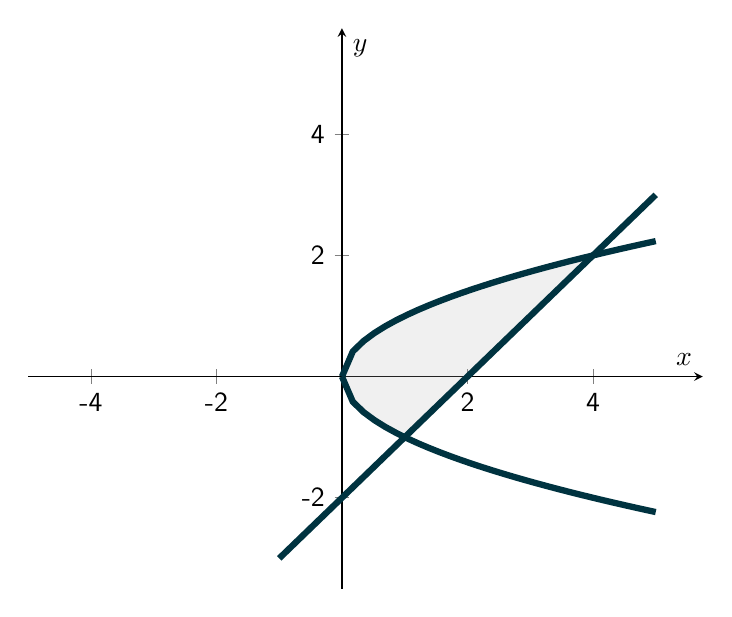
\begin{tikzpicture}[scale=1.25]
            \begin{axis}[
            axis lines = middle, very thick,
            xlabel = {$x$},
            ylabel = {$y$},
            xmin=-5, xmax=5.75,
            ymin=-3.5, ymax=5.75,
            xtick={-4,-2,0,2,4},
            xticklabels={-4,-2,0,2,4},
            ytick={-2,0,2,4},
            yticklabels={-2,0,2,4}        
            ]
            % Curves
            \addplot [name path = A,-,domain = 0:5, line width=0.8mm,DarkBlue,samples = 30] {sqrt(x)} ;
            \addplot [name path = B,-,domain = 0:5, line width=0.8mm,DarkBlue,samples = 30] {-sqrt(x)} ;
            \addplot [name path = C, line width=0.8mm, samples=4, smooth,domain=0:5, DarkBlue] coordinates {(-1,-3)(5,3)};
            % Fill area between paths
            \addplot [black!30, opacity=0.2] fill between [of = A and B, soft clip={domain=0:1}];
            \addplot [black!30, opacity=0.2] fill between [of = A and C, soft clip={domain=1:4}];
            \end{axis}
        \end{tikzpicture}    
    \end{center}   
        
    Thus
    \begin{align}
        \bar y &= \frac{M_x}M = \frac1M \int_{-1}^{2}\int_{y^2}^{y+2} 12y \, dx \, dy
    \end{align} 
    Thus
    \begin{align}
        a &= -1 \\
        b &= 2 \\
        c&= y^2 \\
        d&= y+2 \\
        f(x,y) &= \delta y = 12y
    \end{align}
    }
   \else

   \fi
    
\fi

\ifnum \Version=7
% SHORT SPHERICAL AND CYLINDRICAL EXERCISE
\part Point $P$ has rectangular (Cartesian) coordinates $(x,y,z) = (-6,0,8)$ in $\mathbb R^3$. In cylindrical coordinates, the point is $(r,\theta,z)$, and in spherical coordinates the point is $(\rho, \phi, \theta)$. Where $r=\framebox{\strut\hspace{1cm}}$, $\theta=\framebox{\strut\hspace{2cm}}$, $z=\framebox{\strut\hspace{1cm}}$, $\rho=\framebox{\strut\hspace{2cm}}$, and $\phi=\framebox{\strut\hspace{3cm}}$. 

    \ifnum \Solutions=1 {\color{DarkBlue} \textit{Solutions:} To convert to cylindrical we can use the equation $r^2 = x^2 + y^2$. 
    \begin{align}
        r^2 &= x^2 + y^2 = (-6)^2 + 0^2 = 36 \ \Rightarrow \ r = 6
    \end{align}
    To determine $\theta$ we can use $\tan\theta = y/x$. 
    \begin{align}
        \tan \theta &= \frac{y}{x} = \frac{0}{-6} = 0  \\
        \theta &= \arctan 0 
    \end{align} 
    The point in cylindrical is: 
    \begin{align}
        (r,\theta,z) &= (6,\pi,8) \\
        r &= 6 \\
        \theta &= \pi \\
        z &= 8
    \end{align}
    In spherical, we can start by obtaining $\rho$. 
    \begin{align}
        \rho^2 &= x^2+y^2+z^2\\
        \rho^2 &= (-6)^2 + 0^2 + 8^2 = 36+64 = 100 \\
        \rho &= 10
    \end{align}
    To obtain $\phi$ we can use the equation that relates $x$ to spherical. Using the expression for $x$, and the values that we already have for $x$, $\rho$ and $\theta$:
    \begin{align}
        x &= \rho \sin\phi \cos\theta \\
        -6 &= 10\sin\phi \cos(\pi) \\
        \sin\phi &= \frac{-6}{10 \cos(\pi)}  = \frac{6}{10}\\
        \phi &= \arcsin (6/10)
    \end{align}
    Our coordinates in spherical are
    \begin{align}
        \rho &= 10\\
        \phi &= \arcsin (6/10)\\
        \theta &= \pi
    \end{align}
    Note the following.
    \begin{itemize}
        \item We can, for this exercise, leave un-evaluated trig functions in the answer, because the question didn't specify that you should simplify your answer as much as possible. So it would be ok to leave your answer for $\theta$ as $\arctan 0$ or $\tan^{-1} 0$. 
        \item Our particular textbook uses the convention $(\rho, \phi, \theta)$, not $(\rho, \theta,\phi)$.
    \end{itemize}
    } 
    \else
      
    \fi
    
\fi





\ifnum \Version=8
% SHORT SPHERICAL AND CYLINDRICAL EXERCISE
\part Point $P$ has rectangular (Cartesian) coordinates $(x,y,z) = (4,4,7)$ in $\mathbb R^3$. In cylindrical coordinates, the point is $(r,\theta,z)$, and in spherical coordinates the point is $(\rho, \phi, \theta)$. Where $r=\framebox{\strut\hspace{1cm}}$, $\theta=\framebox{\strut\hspace{2cm}}$, $z=\framebox{\strut\hspace{1cm}}$, $\rho=\framebox{\strut\hspace{2cm}}$, and $\phi=\framebox{\strut\hspace{3cm}}$. 

    \ifnum \Solutions=1 {\color{DarkBlue} \textit{Solutions:} To convert to cylindrical we can use the equation $r^2 = x^2 + y^2$. 
    \begin{align}
        r^2 &= x^2 + y^2 = (4)^2 + 4^2 = 32 \ \Rightarrow \ r = \sqrt{32} = 4\sqrt2
    \end{align}
    It isn't necesssary to simplify to $4\sqrt2$. Then to determine $\theta$ we can use $\tan\theta = y/x$. 
    \begin{align}
        \tan \theta &= \frac{y}{x} = \frac{4}{4} = 1  \\
        \theta &= \arctan \pi/4
    \end{align} 
    The point in cylindrical is: 
    \begin{align}
        (r,\theta,z) &= (4\sqrt2,\pi/4,7) \\
        r &= 4\sqrt2 \\
        \theta &= \pi/4 \\
        z &= 7
    \end{align}
    In spherical, we can start by obtaining $\rho$. 
    \begin{align}
        \rho^2 &= x^2+y^2+z^2\\
        \rho^2 &= (4)^2 + 4^2 + 7^2 = 16+16+49 = 32+49 = 81 \\
        \rho &= 9
    \end{align}
    To obtain $\phi$ we can use the equation that relates $x$ to spherical. Using the expression for $x$, and the values that we already have for $x$, $\rho$ and $\theta$:
    \begin{align}
        x &= \rho \sin\phi \cos\theta \\
        4 &= 9\sin\phi \cos(\pi/4) \\
        \sin\phi &= \frac{4}{9 \cos(\pi/4)}  = \frac{4\sqrt2}{9}\\
        \phi &= \arcsin \left(\frac{4\sqrt2}{9}\right)
    \end{align}
    Note for $\phi$ we can also use:
    \begin{align}
        y &= \rho \sin\phi \sin\theta \\
        4 &= 9\sin\phi \sin(\pi/4) \\
        \sin\phi &= \frac{4}{9 \sin(\pi/4)}  = \frac{4\sqrt2}{9}\\
        \phi &= \arcsin \left(\frac{4\sqrt2}{9}\right)
    \end{align}    
    And we can also use:
    \begin{align}
        z &= \rho \cos\phi  \\
        7 &= 9\cos\phi  \\
        \sin\phi &= \frac{4}{9 \sin(\pi/4)}  = \frac{4\sqrt2}{9}\\
        \phi &= \arccos \left(\frac{7}{9}\right)
    \end{align}      
    Our coordinates in spherical are
    \begin{align}
        \rho &= 9\\
        \phi &= \arcsin \left(\frac{4\sqrt2}{9}\right), \ \textbf{or} \ \phi = \arccos(7/9)\\
        \theta &= \pi/4
    \end{align}
    Note the following.
    \begin{itemize}
        \item We can, for this exercise, leave un-evaluated trig functions in the answer, because the question didn't specify that you should simplify your answer as much as possible. So it would be ok to leave your answer for $\theta$ as $\arctan 1$ or $\tan^{-1} 1$. 
        \item Our particular textbook uses the convention $(\rho, \phi, \theta)$, not $(\rho, \theta,\phi)$.
    \end{itemize}
    } 
    \else
      
    \fi
    
\fi





% 15.6
% CENTROID Y-COORDINATE PARABOLA AND LINE
\ifnum \Version=9
    \part A thin plate with density $\delta=12$ is bounded in the $xy-$plane by $y=3-x^2$ and $y=1-x$. The plate has mass $M$. The $y-$coordinate of the centroid is $\bar y = M_x/M$, where $\displaystyle M_x = \int_A^B \int_C^D f(x,y) \, dy \, dx$,  and $A=\framebox{\strut\hspace{1cm}}$, $B=\framebox{\strut\hspace{1cm}}$, $C=\framebox{\strut\hspace{3cm}}$, $D=\framebox{\strut\hspace{3cm}}$, and $f(x,y) = \framebox{\strut\hspace{3cm}}$. 
    
    \ifnum \Solutions=1 
    {\color{DarkBlue}
    The region is bounded by 
    $$1-x \le y \le 3-x^2$$
    The given curves intersect when 
    \begin{align}
        1-x &= 3-x^2\\
        0 &= x^2-x-2 \\
        &= (x-2)(x+1)
    \end{align}
    The curves intersect at $x=-1,2$. Using $y=1-x$, the intersection points are $(-1,2)$ and $(2,-1)$. The region is shown below. 
    \begin{center}  
        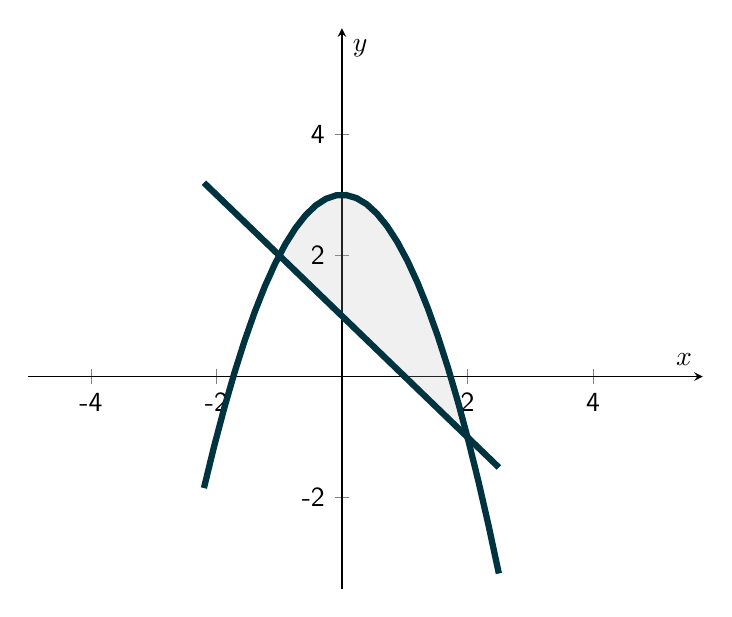
\begin{tikzpicture}[scale=1.25]
            \begin{axis}[
            axis lines = middle, very thick,
            xlabel = {$x$},
            ylabel = {$y$},
            xmin=-5, xmax=5.75,
            ymin=-3.5, ymax=5.75,
            xtick={-4,-2,0,2,4},
            xticklabels={-4,-2,0,2,4},
            ytick={-2,0,2,4},
            yticklabels={-2,0,2,4}        
            ]
            % Curves
            \addplot [name path = A,-,domain = -2.2:2.5, line width=0.8mm,DarkBlue,samples = 30] {3-x^2} ;
            \addplot [name path = C,-,domain = -2.2:2.5, line width=0.8mm,DarkBlue,samples = 4] {1-x} ;
            % Fill area between paths
            \addplot [black!30, opacity=0.2] fill between [of = A and C, soft clip={domain=-1:2}];
            \end{axis}
        \end{tikzpicture}    
    \end{center}   
        
    Thus
    \begin{align}
        \bar y &= \frac{M_x}M = \frac1M \int_{-1}^{2}\int_{1-x}^{3-x^2} 12y \, dy \, dx
    \end{align} 
    Thus
    \begin{align}
        A &= -1 \\
        B &= 2 \\
        C&= 1-x \\
        D&= 3-x^2 \\
        f(x,y) &= \delta y = 12y
    \end{align}
    }
   \else

   \fi
    
\fi
   
    % 13.3 and 13.4
% unit tangent vectors
% arc length
% curvature
% osculating circle
% unit normal

\ifnum \Version=1

\part The unit tangent vector for a curve $\mathbf r(t)$ is $\mathbf T(t) = \langle 0, \cos t, \sin t \rangle$. The unit normal vector is $\mathbf  N = \langle f(t), g(t), g(t) \rangle$, where $f(t) = \framebox{\strut\hspace{2cm}}$, $g(t) = \framebox{\strut\hspace{2cm}}$, $h(t) =\framebox{\strut\hspace{2cm}}$. 

\ifnum \Solutions=1 {\color{DarkBlue} \textit{Answer:} \textit{Solutions:} The normal vector is

\begin{align}
    \mathbf N &= \frac{d\mathbf T/dt}{|d\mathbf T/dt|} 
\end{align}
And
\begin{align}
    \mathbf T'(t) &= \langle 0,-\sin t, \cos t \rangle \\
    |\mathbf T'(t) | &= \sqrt{ 0 +(-\sin t)^2 + (\cos t)^2} =1\\
    \mathbf N &= \frac{d\mathbf T/dt}{|d\mathbf T/dt|} = \langle 0, - \sin(t),  \cos(t) \rangle
\end{align}
} 
\else
\fi        
\fi

\ifnum \Version=2

\part The velocity vector of an object moving on the curve $\mathbf r(t)$ is $\mathbf v(t) = \langle 4\cos (2t), 4\sin (2t) , 3 \rangle$ for $t>0$. The speed of the object for $t>0$ is $s(t) = |\mathbf v | = \framebox{\strut\hspace{1cm}}$. The unit tangent vector for $t>0$ is $\mathbf T = \langle f(t), g(t) , h(t) \rangle$, where $f(t) = \framebox{\strut\hspace{1.5cm}}$, $g(t) = \framebox{\strut\hspace{1.5cm}}$, $h = \framebox{\strut\hspace{1cm}}$. The curvature is $\kappa = \framebox{\strut\hspace{1cm}}$. 

\ifnum \Solutions=1 {\color{DarkBlue} \textit{Answer:} \textit{Solutions:} The speed is the magnitude of the given velocity vector and is
\begin{align}
    s &= |\mathbf v | =  \sqrt{(4\cos2t)^2 + (4\sin2t)^2 + 3^2 } = \sqrt{4^2 (\cos ^2 2 t + \sin^2 2t) + 3^2} = \sqrt{16 + 9} = 5
\end{align}
The unit tangent vector is 
\begin{align}
    \mathbf T &= \frac{\mathbf v}{|\mathbf v|} = \langle \frac{4}{5}\cos(2 t) , \frac 45 \sin (2t), \frac35 \rangle
\end{align}
For curvature we also need
\begin{align}
    \frac{d\mathbf T}{dt } &= \langle -\frac85 \sin 2t, \frac85 \cos 2t,0 \rangle \\
    \left | \frac{d\mathbf T}{dt } \right| &= \sqrt{ \left(-\frac85\sin 2t\right)^2 +   \left(\frac85 \cos 2 t\right)^2 } = \frac85
\end{align}
The curvature is
\begin{align}
    \kappa = \frac{1}{|\mathbf v |}\left| \frac{d\mathbf T}{dt}\right| = \frac{1}{5} \cdot \frac{8}{5} = \frac{8}{25}
\end{align}
} 
\else
\fi        
\fi


\ifnum \Version=3

\part A plane curve $\mathbf r(t)$ has curvature $\kappa = \frac{1}{8}$ at $\mathbf r(t_0) = \langle 15, 2 \rangle$, and the unit normal vector at $t=t_0$ is $\mathbf  N = \mathbf j = \langle 0, 1 \rangle$. The equation of the osculating circle at $t=t_0$ is \framebox{\strut\hspace{3.5cm}}.

\ifnum \Solutions=1 {\color{DarkBlue} \textit{Answer:} \textit{Solutions:} Recall that The circle of curvature, or osculating circle, at a point $P$ on a plane curve where $\kappa \ne 0$ is the circle in the plane of the curve that

\begin{enumerate}
    \item is tangent to the curve at P (has the same tangent line the curve has)
    \item has the same curvature the curve has at P
    \item lies toward the concave or inner side of the curve
\end{enumerate}
The \textbf{radius of curvature} of the curve at P is the radius of the circle of curvature, which is $\frac{1}{\kappa}$. So to obtain the radius, we calculate $\kappa$ and take the reciprocal. The \textbf{center} of the osculating circle of the curve at P lies on the inner side of the curve, and the unit normal points in the direction of the inner side of the planar curve. 

So for this problem we have a circle with radius $1/\kappa = 8$, and whose centre is 8 units away from the point $(15,2)$ in the direction of $\mathbf N$. The circle has equation
$$(x-15)^2 + (y-10)^2 = 8^2$$
} 
\else
  
\fi        
\fi




\ifnum \Version=4

\part The velocity vector for an object moving on the curve $\mathbf r(t)$ is $\mathbf v(t) = \langle t\cos t, t\sin t \rangle$. The speed of the object for $t>0$ is $s(t) = \framebox{\strut\hspace{1cm}}$. The unit tangent vector for $t>0$ is $\mathbf T = \langle f(t), g(t) \rangle$, where $f(t) = \framebox{\strut\hspace{2cm}}$, $g(t) = \framebox{\strut\hspace{2cm}}$. 

\ifnum \Solutions=1 {\color{DarkBlue} \textit{Answer:} \textit{Solutions:} The speed is the magnitude of the velocity vector and is
\begin{align}
    s &= |\mathbf v | = \sqrt{(t\cos t)^2 + (t\sin t)^2 } = \sqrt{t^2 (\cos ^2 t + \sin^2 t)} = |t|
\end{align}
But we are told that $t>0$ so we can use $|t| = t$. The unit tangent vector is 
\begin{align}
    \mathbf T &= \frac{\mathbf v}{|\mathbf v|} = \langle \cos t, \sin t \rangle
\end{align}
} 
\else
\fi        
\fi

\ifnum \Version=5

\part A plane curve $\mathbf r(t)$ has curvature $\kappa = \frac{1}{4}$ at the point $\mathbf r(t_0) = 3\mathbf i + 5\mathbf j$, and the unit normal vector at $t_0$ is $\mathbf  N = \mathbf i = \langle1,0\rangle$. The equation of the osculating circle at $t=t_0$ is \framebox{\strut\hspace{3.5cm}}.

\ifnum \Solutions=1 {\color{DarkBlue} \textit{Answer:} \textit{Solutions:} Recall that The circle of curvature, or osculating circle, at a point $P$ on a plane curve where $\kappa \ne 0$ is the circle in the plane of the curve that

\begin{enumerate}
    \item is tangent to the curve at P (has the same tangent line the curve has)
    \item has the same curvature the curve has at P
    \item lies toward the concave or inner side of the curve
\end{enumerate}
The \textbf{radius of curvature} of the curve at P is the radius of the circle of curvature, which is $\frac{1}{\kappa}$. So to obtain the radius, we calculate $\kappa$ and take the reciprocal. The \textbf{center} of the osculating circle of the curve at P lies on the inner side of the curve, and the unit normal points in the direction of the inner side of the planar curve. 

So for this problem we have a circle with radius $1/\kappa = 4$, and whose centre is 4 units away from the point $(3,5)$ in the direction of $\mathbf N$. The circle has equation
$$(x-7)^2 + (y-5)^2 = 4^2$$
} 
\else
  
\fi        
\fi


\ifnum \Version=6

\part The velocity vector for an object moving on the curve $\mathbf r(t)$ is $\mathbf v(t) = \langle 4t\cos t, 4t\sin t \rangle$ for $t>0$. The speed of the object for $t>0$ is $s(t)  = |\mathbf v | = \framebox{\strut\hspace{1cm}}$. The unit tangent vector for $t>0$ is $\mathbf T = \langle f(t), g(t) \rangle$, where $f(t) = \framebox{\strut\hspace{1.5cm}}$, $g(t) = \framebox{\strut\hspace{1.5cm}}$. The curvature is $\kappa = \framebox{\strut\hspace{1cm}}$. 

\ifnum \Solutions=1 {\color{DarkBlue} \textit{Answer:} \textit{Solutions:} The speed is the magnitude of the given velocity vector and is
\begin{align}
    s &= |\mathbf v | =  \sqrt{(4t\cos t)^2 + (4t\sin t)^2 } = \sqrt{4^2t^2 (\cos ^2 t + \sin^2 t)} = 4|t|
\end{align}
But we are told that $t>0$ so we can assume $|t| = t$. The unit tangent vector is 
\begin{align}
    \mathbf T &= \frac{\mathbf v}{|\mathbf v|} = \langle \cos t, \sin t \rangle
\end{align}
We need
\begin{align}
    \frac{d\mathbf T}{dt } &= \langle -\sin t, \cos t \rangle \\
    \left | \frac{d\mathbf T}{dt } \right| &= \sqrt{ (-\sin t)^2 +   \cos^2 t } = 1
\end{align}
The curvature is
\begin{align}
    \kappa = \frac{1}{|\mathbf v |}\left| \frac{d\mathbf T}{dt}\right| = \frac{1}{4t} 
\end{align}
} 
\else
\fi        
\fi



\ifnum \Version=7

\part The velocity vector of an object moving on the curve $\mathbf r(t)$ is $\mathbf v(t) = \langle 3\cos (2t), 3\sin (2t) \rangle$ for $t>0$. The speed of the object for $t>0$ is $s(t) = |\mathbf v | = \framebox{\strut\hspace{1.5cm}}$. The unit tangent vector for $t>0$ is $\mathbf T = \langle f(t), g(t)  \rangle$, where $f(t) = \framebox{\strut\hspace{2cm}}$, and $g(t) = \framebox{\strut\hspace{2cm}}$.  The curvature for $t>0$ is \framebox{\strut\hspace{1.5cm}}. 

\ifnum \Solutions=1 {\color{DarkBlue} \textit{Answer:} \textit{Solutions:} The speed is the magnitude of the given velocity vector and is
\begin{align}
    s &= |\mathbf v | =  \sqrt{(3\cos t)^2 + (3\sin t)^2  } = \sqrt{3^2 (\cos ^2 t + \sin^2 t) + 3^2} = \sqrt{ 9} = 3
\end{align}
The unit tangent vector is 
\begin{align}
    \mathbf T &= \frac{\mathbf v}{|\mathbf v|} 
    = \langle \frac{3}{3}\cos(2 t) , \frac 33 \sin (2t) \rangle 
    = \langle \cos(2 t) ,  \sin (2t) \rangle
\end{align}
For curvature we also need
\begin{align}
    \frac{d\mathbf T}{dt } &= \langle -2 \sin 2t, 2 \cos 2t\rangle \\
    \left | \frac{d\mathbf T}{dt } \right| &= \sqrt{ \left(-2\sin 2t\right)^2 +   \left(2 \cos 2 t\right)^2 } = 2
\end{align}
The curvature is
\begin{align}
    \kappa = \frac{1}{|\mathbf v |}\left| \frac{d\mathbf T}{dt}\right| = \frac{1}{3} \cdot 2 = \frac{2}{3}
\end{align}
} 
\else
\fi        
\fi


\ifnum \Version=8

\part A plane curve $\mathbf r(t)$ has curvature $\kappa = \frac{1}{4}$ at $\mathbf r(t_0) = \langle 5, 3 \rangle$, and the unit normal vector at $t=t_0$ is $\mathbf  N = \mathbf j = \langle 0, 1 \rangle$. The equation of the osculating circle at $t=t_0$ is \framebox{\strut\hspace{3.5cm}}.

\ifnum \Solutions=1 {\color{DarkBlue} \textit{Answer:} \textit{Solutions:} Recall that The circle of curvature, or osculating circle, at a point $P$ on a plane curve where $\kappa \ne 0$ is the circle in the plane of the curve that

\begin{enumerate}
    \item is tangent to the curve at P (has the same tangent line the curve has)
    \item has the same curvature the curve has at P
    \item lies toward the concave or inner side of the curve
\end{enumerate}
The \textbf{radius of curvature} of the curve at P is the radius of the circle of curvature, which is $\frac{1}{\kappa}$. So to obtain the radius, we calculate $\kappa$ and take the reciprocal. The \textbf{center} of the osculating circle of the curve at P lies on the inner side of the curve, and the unit normal points in the direction of the inner side of the planar curve. 

So for this problem we have a circle with radius $1/\kappa = 4$, and whose centre is 4 units away from the point $(5,3)$ in the direction of $\mathbf N$. The circle has equation
$$(x-5)^2 + (y-7)^2 = 4^2$$
} 
\else
  
\fi        
\fi






\ifnum \Version=9

\part The velocity vector of an object moving on the curve $\mathbf r(t)$ is $\mathbf v(t) = \langle t, 3 \rangle$ for $t>0$. The speed of the object at $t=2$ is $s(2) = |\mathbf v(2) | = \framebox{\strut\hspace{1.75cm}}$. The unit tangent vector at $t=2$ is $\mathbf T(2) = \langle c_1 ,c_2  \rangle$, where $c_1 = \framebox{\strut\hspace{1.75cm}}$, $c_2 = \framebox{\strut\hspace{1.75cm}}$. The curvature is $\framebox{\strut\hspace{1.75cm}}$. 

\ifnum \Solutions=1 {\color{DarkBlue} \textit{Answer:} \textit{Solutions:} The speed is the magnitude of the given velocity vector and is
\begin{align}
    s &= |\mathbf v | =  \sqrt{( t)^2 + (3)^2  } = \sqrt{t^2+9}\\
    s(2) &= \sqrt{2^2+9} = \sqrt{13}
\end{align}
We also need the unit tangent vector at $t=2$. 
\begin{align}
    \mathbf T (t) &= \frac{\mathbf v}{|\mathbf v|} = \frac{t\mathbf i + 3\mathbf j}{\sqrt{t^2+9}} \\
    \mathbf T (2) &= \frac{2\mathbf i + 3\mathbf j}{\sqrt{2^2+9}}  
    = \langle \frac{2}{\sqrt{13}} , \frac {3}{\sqrt{13}}  \rangle \\
    c_1 &= \frac{2}{\sqrt{13}}\\
    c_2 &= \frac{3}{\sqrt{13}}
\end{align}
The curvature is zero because the motion is along a straight line. 
\begin{align}
    \kappa = 0
\end{align}
} 
\else
\fi        
\fi

\ifnum \Version=10

\part A plane curve $\mathbf r(t)$ has curvature $\kappa = \frac{1}{10}$ at $\mathbf r(t_0) = \langle 5, 0 \rangle$, and the unit normal vector at $t=t_0$ is $\mathbf  N = \mathbf j = \langle 0, 1 \rangle$. The equation of the osculating circle at $t=t_0$ is \framebox{\strut\hspace{3.5cm}}.

\ifnum \Solutions=1 {\color{DarkBlue} \textit{Answer:} \textit{Solutions:} Recall that The circle of curvature, or osculating circle, at a point $P$ on a plane curve where $\kappa \ne 0$ is the circle in the plane of the curve that

\begin{enumerate}
    \item is tangent to the curve at P (has the same tangent line the curve has)
    \item has the same curvature the curve has at P
    \item lies toward the concave or inner side of the curve
\end{enumerate}
The \textbf{radius of curvature} of the curve at P is the radius of the circle of curvature, which is $\frac{1}{\kappa}$. So to obtain the radius, we calculate $\kappa$ and take the reciprocal. The \textbf{center} of the osculating circle of the curve at P lies on the inner side of the curve, and the unit normal points in the direction of the inner side of the planar curve. 

So for this problem we have a circle with radius $1/\kappa = 10$, and whose centre is 10 units away from the point $(5,0)$ in the direction of $\mathbf N$. The circle has equation
$$(x-5)^2 + (y-10)^2 = 10^2$$
} 
\else
  
\fi        
\fi
   
\end{parts}

\newpage \question[0.25] \ID
% CHANGE OF VARIABLE (15.8)
% OR APPLICATION (15.6)
% OR TRIPLE CARTESIAN (15.5) 

\ifnum \Version=1
% CENTROID
% BASED ON THOMAS EXERCISES, 15.6 #1
% SUFFICIENT FOR A PRACTICE EXAM
\question[6] A thin plate of density $\delta(x,y) = 12x$ is bounded by the lines $x = 0, y = x$, and the parabola $y = x^2-6$ in the first quadrant. 
\begin{parts} 
    \part Determine the mass of the plate, $M$. Please show your work. 
    \ifnum \Solutions=1 
    {\color{DarkBlue} \textit{Solutions:}
    Curves intersect when $$x = x^2-6 \quad \Rightarrow \quad 0 = x^2 - x - 6 = (x-3)(x+2)$$
    Or $x=3, -2$. We can ignore $x=-2$ because the region is the first quadrant. Curves intersect at the point $(3,3)$, and 
    \begin{align}
        0 \le y \le 3, \quad y \le x \le \sqrt{y+6}
    \end{align}
    The mass is
    \begin{align}
        M &= \int_0^3 \int_y^{\sqrt{y+6}} \delta \, dx \, dy \\
        &= \int_0^3 \int_y^{\sqrt{y+6}} 12x \, dx \, dy \\
        &= \int_0^3  \left. 6x^2 \right|_{x=y}^{x=\sqrt{y+6}} \, dy \\
        &= \int_0^3 6(y + 6 - y^2) \, dy \\
        &= \int_0^3 6y + 36 - 6y^2 \, dy \\
        &= \left. (3y^2 + 36y - 2y^3 ) \right|_0^3 \, dy \\
        &= 27 + 108 - 54 \\
        &= 81
    \end{align}
    }
    \else 
    \vspace{16cm}
    \fi
    \part Use your results from the previous part to set up an integral that can be used to determine the $x-$coordinate of the center of mass of the plate. You do not need to evaluate your integral. 
    \ifnum \Solutions=1 {\color{DarkBlue} \textit{Solutions:} the $x-$coordinate of the center of mass, $\bar x$, is
    \begin{align}
    \bar x &= \frac{M_y}{M} = \frac{1}{81} \int_0^3 \int_y^{\sqrt{y+6}} 12x^2 \, dx \, dy 
    \end{align}
    } 
    \else
      
    \fi
    \end{parts} 
\fi
    





\ifnum \Version=2
% LONGISH CHANGE OF VARIABLE
% VERBATUM FROM SPRING 2022 QUIZ
% hand written solution only
% SUFFICIENT FOR A PRACTICE EXAM
\question[6] Consider the double integral

$$I=\iint_R \frac{x+2y}{2y-x} dA$$

where $R$ is the parallelogram with vertices $(-3,1), (-1,0), (-1,2), (1,1)$. Our goal is to determine the area of the parallelogram using the transform below. 
$$u=x+2y, \qquad v = -x +2y$$ 
Please show your work for the following. 
\begin{parts} 
    \part Use the given transform to calculate the Jacobian of the transform, $J = \partial x(u,v)/\partial y(u,v)$. 
    \ifnum \Solutions=1 
    \else 
    \vspace{8 cm}
    \fi
    \part Use your results from Part (a) and the given transform to transform the double integral. You do not need to evaluate your integral. 
\end{parts} 

\ifnum \Solutions=1 {\color{DarkBlue} \textit{Solutions:} the integral after the transform is $$\displaystyle \frac14 \int_1^5\int_{-1}^3 \frac uv \, du \, dv$$
A screen capture of a hand-written solution from a previous offer of MATH 2551 is below. 
    \begin{figure}[h]
    \centering
    \includegraphics[width=16cm]{202302/Exam3/Images/ImgE3.OR.06.png}
    \end{figure}  
    
    } 
   \else
      
   \fi
    
\fi

\ifnum \Version=3
% CENTROID
% BASED ON THOMAS EXERCISES, 15.6 #1
% SUFFICIENT FOR A PRACTICE EXAM
\question[6] A thin plate with density $\delta(x,y) = 24y$ is bounded by the lines $x = 0, x=2y$, and the parabola $x=y^2$ in the first quadrant. 
\begin{parts} 
    \part Determine the mass of the plate, $M$. Please show your work. 
    
    \ifnum \Solutions=1 
    {\color{DarkBlue} \textit{Solutions:}
    Curves intersect when $$2y = y^2 \quad \Rightarrow \quad 0 = y^2-2y = y(y-2)$$
    Or $y=0,2$. Curves intersect at the points $(0,0)$, $(4,2)$. 
    The mass is
    \begin{align}
        M = \int_0^4 \int_{x/2}^{\sqrt{x}} \delta \, dy \, dx 
        &= \int_0^4 \int_{x/2}^{\sqrt{x}} 24y \, dy \, dx \\
        &= \int_0^4  \left. 12y^2 \right|_{y=x/2}^{y=\sqrt{x}} \, dx \\
        &= 12 \int_0^4 (x-\frac{x^2}{4}) \, dx \\
        &= 12 \left. (\frac{x^2}{2} - \frac{x^3}{12} ) \right|_0^4 \, dy \\
        &= 12 (\frac{16}{2} - \frac{64}{12}) \\
        &= 96 - 64\\
        &= 32
    \end{align}
    \textbf{An Alternate Solution}\\
    Another way to approach this problem is to use the integration order $dx\,dy$. In this case the double integral becomes
    \begin{align}
        M = \int_0^2 \int_{y^2}^{2y} \delta \, dx \, dy
        &= \int_0^2 \int_{y^2}^{2y} 24y \, dx \, dy \\
        &= 24\int_0^2  \left. yx \right|_{x=y^2}^{x=2y} \, dy \\
        &= 24 \int_0^2 (2y^2 - y^3) \, dy \\
        &= 24 \left. (\frac{2y^3}{3} - \frac{y^4}{4} ) \right|_0^2 \, dy \\
        &= 24 (\frac{16}{3} - \frac{16}{4}) \\
        &= \frac{24\cdot16}{3} - 24\cdot 4 \\
        &= 8\cdot16 - 96 \\
        &= 128 - 96 \\
        &= 32
    \end{align}    
    }
    \else 
    \vspace{14cm}
    \fi
    \part Use your results from the previous part to set up an integral that can be used to determine the $x-$coordinate of the center of mass of the plate. You do not need to evaluate your integral. 
    \ifnum \Solutions=1 {\color{DarkBlue} \textit{Solutions:} the $x-$coordinate of the center of mass, $\bar x$, is
    \begin{align}
    \bar x &= \frac{M_y}{M} = \frac{1}{32} \int_0^4 \int_{x/2}^{\sqrt{x}} 24xy \, dy \, dx
    \end{align}
    \textbf{An Alternate Solution}\\    
    It is also ok to use the integration order $dx\,dy$. In this case the double integral becomes
    \begin{align}
    \bar x &= \frac{M_y}{M} = \frac{1}{32} \int_0^2 \int_{y^2}^{2y} 24xy \, dx \, dy 
    \end{align}
    } 
    \else
      
    \fi
    \end{parts} 
\fi

\ifnum \Version=4
% VERSION B
% LONG CHANGE OF VARIABLE
% BASED ON AN EXAMPLE FROM THOMAS
% SECTION 15.8 FROM THOMAS
\question[6] Consider the double integral

$$I= 9 \iint_R (y-2x)^2 \sqrt{x+y} \, dA$$

where $R$ is the region in the first quadrant bounded by the lines $x=0$, $y=0$, and $y=1-x$. Our goal is to determine the area of $R$ using the transform below. 
$$u=x+y, \qquad v = y-2x$$ 
Please show your work for the following. 
\begin{parts} 
    \part Use the given transform to calculate the Jacobian of the transform, $J = \partial x(u,v)/\partial y(u,v)$. 
    \ifnum \Solutions=1 {\color{DarkBlue} \textit{Solutions:} Solving for $x$ and $y$ using an augmented matrix,
    \begin{align}
        \begin{pmatrix} 1 & 1 & u \\-2 & 1 & v\end{pmatrix} 
        \sim \begin{pmatrix} 1 & 1 & u \\0 & 3 & 2u+v\end{pmatrix} 
        \sim \begin{pmatrix} 1 & 0 & u/3 - v/3 \\0 & 1 & 2u/3+v/3 \end{pmatrix} 
    \end{align}
    Thus
    \begin{align}
        x &= \frac13(u-v), \ y = \frac13(2u+v) \\
        J(u,v) & = \begin{vmatrix} \DXDU & \DXDV \\[8pt] \DYDU & \DYDV \end{vmatrix} = \begin{vmatrix} 1/3 & -1/3 \\ 2/3 & 1/3 \end{vmatrix} = 1/9 + 2/9 = 1/3
    \end{align}
    }
    \else 
    \vspace{8 cm}
    \fi
    \part Use the given transform and your results from Part (a) to convert the double integral into a double integral over a region in the $uv-$plane. You do not need to evaluate your integral. 
    \ifnum \Solutions=1 {\color{DarkBlue} \textit{Solutions:} Converting each of the boundaries in the $xy-$plane into the $uv-$plane we obtain
        \begin{align}
            x+y &= 1 \quad \Rightarrow \quad \frac13(u-v) + \frac13(2u+v) = 1 &&\Rightarrow \quad u = 1\\
            x&=0 \quad \Rightarrow \quad \frac13(u-v) = 0 &&\Rightarrow \quad v = u\\
            y&= 0 \quad \Rightarrow \quad \frac13(2u+v) = 0 &&\Rightarrow \quad v = -2u
        \end{align}
        The region is described by either of the following relations:
        \begin{align}
            S_1: & \quad 0 \le u \le 1, \quad -2u \le v \le u \\
            S_2: & \quad -2 \le v \le 0, \quad -v/2 \le u \le 1, \ \text{and } 0 \le v \le 1, \quad v \le u \le 1
        \end{align}
        The first set of inequalities requires only a single double integral, but it is ok to set up two double integrals. If using $S_1$, we use $dv\,du$ and obtain
        \begin{align}
            I= 9 \iint_R (y-2x)^2 \sqrt{x+y} \, dA = 9 \int_0^1 \int_{-2u}^u v^2u^{1/2} \frac13 \,dv\,du
        \end{align}
        If using $S_2$, we use $du\,dv$ and obtain
        \begin{align}
            I= 9 \iint_R (y-2x)^2 \sqrt{x+y} \, dA 
            = 9 \int_{-2}^0 \int_{-v/2}^1 v^2u^{1/2} \frac13 \,du\,dv
            + 9 \int_{0}^1 \int_{v}^1 v^2u^{1/2} \frac13 \,du\,dv
        \end{align}        
        } 
       \else
          
       \fi
    \end{parts} 

    \fi



\ifnum \Version=5
    % USE FOR VERSION B
    % LONG CYLINDRICAL WITH APPLICATION TO MASS WITH VARYING DENSITY
    % FROM 15.8
    \question[6] An object $D$ lying in the first octant is bounded below by the $xy-$plane, above by the plane $z=3+4y$, and by the cylinder $x^2+y^2 = 4$. The density of the object at any point in $D$ is equal to the distance from the point to the $z$-axis.  Please show your work for the following.
    
    \begin{parts} 
    \part Use cylindrical coordinates to calculate the total of mass of the object, $M$. Please show your work. 
    
    \ifnum \Solutions=1 {\color{DarkBlue} The object is only in the first octant so $$0 \le \theta \le \pi/2$$ Using $\delta = \sqrt{x^2+y^2} = r$, the $z-$coordinate of the center of mass is computed using 
    \begin{align}
        M &= \iiint_D  \delta \, dV \\
        &= \int_0^{\pi/2} \int_0^2 \int_0^{3+4r\sin\theta}  \delta(r,\theta) \, r\, dz\,dr\,d\theta\\
        &= \int_0^{\pi/2} \int_0^2 \int_0^{3+4r\sin\theta}   r^2 \, dz\,dr\,d\theta\\
        &= \int_0^{\pi/2} \int_0^2    r^2 \, (3+4r\sin\theta) \,dr\,d\theta \\
        &= \int_0^{\pi/2} \int_0^2     \, (3r^2+4r^3\sin\theta) \,dr\,d\theta \\
        &= \int_0^{\pi/2}  \left. \, (r^3+r^4\sin\theta) \right|_{r=0}^{r=2} d\theta \\
        &= \int_0^{\pi/2}  (8 + 16\sin\theta) d\theta \\
        &=  \left. (8\theta - 16\cos\theta) \right|_0^{\pi/2} \\
        &=  (4\pi - 0) - (0 - 16) \\
        &= 4\pi + 16
    \end{align}
    
    } 
    \else
        \vspace{14cm}
    \fi
    
    \part Use your results from the previous part to set up a triple integral in cylindrical coordinates that can be used to determine the $z-$coordinate of the center of mass of the object. You do not need to evaluate your integral. 

    \ifnum \Solutions=1 {\color{DarkBlue} \textit{Solutions:} the $z-$coordinate of the center of mass, $\bar x$, is
    \begin{align}
    \bar z &= \frac{M_{xy}}{M} = \frac{1}{16\pi+16} \int_0^{\pi/2} \int_0^2 \int_0^{3+4r\sin\theta}  z \, \delta(r,\theta) \, r\, dz\,dr\,d\theta
    \end{align}
    } 
    \else
      
    \fi
    \end{parts} 
\fi


% TRANSFORM: SOLVE FOR X & Y, BOUNDARIES, EVALUATE, TRIANGLES
% VERSION A
\ifnum \Version=6
    \question[6] Consider the transform $u=x+y$ and $v=4x+5y$, and the integral $\displaystyle I = \iint_{R}  \,dxdy$. Region $R$ is the triangle in the $xy$-plane bounded by $x+y=0$, $4x+5y=0$, $6x+7y=4$. The transform maps $R$ to region $G$ in the $uv-$plane.  Please show your work for the following.

    \begin{enumerate}
        \item[a)] Solve the system, $u=x+y$ and $v=4x+5y$, for $x$ and $y$ in terms of $u$ and $v$.
            \ifnum \Solutions=1 {\color{DarkBlue} \\[12pt] 
            \textbf{Solutions:}
            We can use the expressions for $u$ and $v$ as an augmented matrix and row reduce. 
            \begin{align}
                \begin{pmatrix} 1 & 1 & u \\ 4 & 5 & v\end{pmatrix} 
                \sim \begin{pmatrix} 1 & 1 & u \\0 & 1 & v - 4u \end{pmatrix} 
                \sim \begin{pmatrix} 1 & 0 & 5u - v \\ 0 & 1 & v - 4u \end{pmatrix} 
            \end{align}
            Thus $x = 5u - v$, and $y = v - 4u$. 
            } 
            \else 
            \vspace{5cm}
            \fi
        \item[b)] Transform the boundaries of $R$ to the $uv-$plane. In other words, determine the boundaries of $G$ in terms of $u$ and $v$. 
            \ifnum \Solutions=1 {\color{DarkBlue} \\[12pt] 
            \textbf{Solutions:} the three lines are transformed below. 
            \begin{itemize}
                \item The line $x+y=0$ becomes $u=0$. 
                \item The line $4x+5y=0$ becomes $v=0$. 
                \item The line $6x+7y=4$ is: 
                \begin{align}
                    6x+7y &=4 \\
                    6\cdot(5u-v) + 7\cdot(v-4u) &= 4\\
                    30u -28u -6v+7v &=4 \\
                    v &= 4 -2u
                \end{align}
            \end{itemize}
            } 
        \else 
        \vspace{5cm}
        \fi        
            
        \item[c)] Use the given transformation and your results from parts (a) and (b) to set up a double integral that in the $uv-$plane that is equal to $I$. Do not evaluate the integral. You also do not need to calculate the Jacobian and may use that the Jacobian of the transform is $J(u,v) = 1$.
            \ifnum \Solutions=1 {\color{DarkBlue} \\[12pt] 
            \textbf{Solutions:}
            \begin{align}
                \iint_{R} \,dx\,dy
                &= \iint_{G}  \left| J(u,v) \right| \,dv\,du 
                = \int_0^2\int_{0}^{4-2u}  \left| 1 \right| \,dv\,du 
                = \int_0^2\int_{0}^{4-2u} \,dv\,du
            \end{align}
            Note the following.
            \begin{itemize}
                \item We did not need to compute the Jacobian but it is computed as follows. 
                $$J 
                = \begin{vmatrix} x_u & x_v \\ y_u & y_v \end{vmatrix} 
                = \begin{vmatrix} 5 & -1 \\ -4 & 1\end{vmatrix} 
                = 5 - 4
                = 1$$
                \item             We did not need to evaluate the integral but if we did:
            \begin{align}
                I = \int_0^2\int_{0}^{4-2u}  \left| 1 \right| \,dv\,du
                = 1 \int_0^2 (4-2u) \,du
                =  \left. 4u - u^2 \right|_0^2 
                = 4
            \end{align}
            \item It is also ok to use the other integration order: $I = \int_0^4\int_0^{2-v/2} \, du \, dv$.
            \end{itemize}
            } 
            \else 
            \fi        
    \end{enumerate}
 
\fi 



% TRANSFORM: SOLVE FOR X & Y, BOUNDARIES, EVALUATE, PARALLELOGRAM
% VERSION A
\ifnum \Version=7
    \question[6] Consider the integral $\displaystyle I = 2\iint_{R} x-4y \,dx\,dy$, where $R$ is the parallelogram in the $xy$-plane bounded by $x-4y=2$, $x-4y=1$, $3y-x=3$, $3y-x=6$. Suppose the transform $u=x-4y$ and $v=3y-x$, maps region $R$ to region $G$ in the $uv-$plane.  Please show your work for the following.

    \begin{enumerate}
        \item[a)] Solve the system, $u=x-4y$ and $v=3y-x$, for $x$ and $y$ in terms of $u$ and $v$.
            \ifnum \Solutions=1 {\color{DarkBlue} \\[12pt] 
            \textbf{Solutions:}
            We can use the expressions for $u$ and $v$ as an augmented matrix and row reduce. 
            \begin{align}
                \begin{pmatrix} 1 & -4 & u \\ -1 & 3 & v\end{pmatrix} 
                \sim \begin{pmatrix} 1 & -4 & u \\0 & -1 & v + u\end{pmatrix} 
                \sim \begin{pmatrix} 1 & 0 & -3u-4v\\0 & 1 & -u-v\end{pmatrix} 
            \end{align}
            Thus
            \begin{align}
                x &=  -3u-4v\\
                y &= -u-v
            \end{align}

            } 
            \else 
            \vspace{5cm}
            \fi
        \item[b)] Transform the boundaries of $R$ to the $uv-$plane. In other words, determine the boundaries of $G$ in terms of $u$ and $v$. 
            \ifnum \Solutions=1 {\color{DarkBlue} \\[12pt] 
            \textbf{Solutions:} the four lines are transformed below. 
            \begin{itemize}
                \item The line $x-4y=2$ becomes $u=2$. 
                \item The line $x-4y=1$ becomes $u=1$. 
                \item The line $3y-x=3$ becomes $v=3$. 
                \item The line $3y-x=6$ becomes $v=6$. 
            \end{itemize}
            } 
        \else 
        \vspace{5cm}
        \fi        
            
        \item[c)] Use the given transformation and your results from parts (a) and (b) to set up a double integral that in the $uv-$plane that is equal to $I$. Do not evaluate the integral. You also do not need to calculate the Jacobian and may use that the Jacobian of the transform is  $J(u,v) = -1$. 
            \ifnum \Solutions=1 {\color{DarkBlue} \\[12pt] 
            \textbf{Solutions:}
            \begin{align}
                \iint_{R} 2x-8y \,dx\,dy
                = \iint_{G} 2u \left| J(u,v) \right| \,du\,dv
                = \int_3^6\int_{1}^2 2u \left| -1 \right| \,du\,dv
                = \int_3^6\int_{1}^2 2u \,du\,dv
            \end{align}
            Note the following.
            \begin{itemize}
                \item We did not need to evaluate the integral, but if we did: 
                \begin{align}
                \iint_{R} 2x-8y \,dx\,dy
                &= \iint_{G} 2u \left| J(u,v) \right| \,du\,dv\\
                &= \int_3^6\int_{1}^2 2u \left| -1 \right| \,du\,dv\\
                &= \int_3^6\left. u^2 \right|_{1}^2 \,dv\\
                &= \int_3^6 3 \,dv\\
                &= 3 \cdot(6 -3) \\
                &= 9
            \end{align}
            \end{itemize}
            } 
            \else 
            \fi        
    \end{enumerate}
 
\fi 




% TRANSFORM: SOLVE FOR X & Y, BOUNDARIES, EVALUATE
% VERSION B
\ifnum \Version=8
    \question[6] Consider the transform $u=x-y$ and $v=4y-2x$, and the integral $\displaystyle I = \iint_{R} \,dxdy$, where $R$ denotes the triangle in the $xy$-plane bounded by $x-y=2$, $4y-2x=0$, $3y=2x$. The transform maps region $R$ to region $G$ in the $uv-$plane.  Please show your work for the following.

    \begin{enumerate}
        \item[a)] Solve the system, $u=x-y$ and $v=4y-2x$, for $x$ and $y$ in terms of $u$ and $v$.
            \ifnum \Solutions=1 {\color{DarkBlue} \\[12pt] 
            \textbf{Solutions:}
            We can use the expressions for $u$ and $v$ as an augmented matrix and row reduce. 
            \begin{align}
                \begin{pmatrix} 1 & -1 & u \\ -2 & 4 & v\end{pmatrix} 
                \sim \begin{pmatrix} 1 & -1 & u \\0 & 2 & v + 2u\end{pmatrix} 
                \sim \begin{pmatrix} 1 & -1 & u\\0 & 1 & u+v/2\end{pmatrix} 
                \sim \begin{pmatrix} 1 & 0 & 2u+v/2\\0 & 1 & u+v/2\end{pmatrix} 
            \end{align}
            Thus $x = 2u+v/2$, and $y = u + \frac{v}{2}$. 
            } 
            \else 
            \vspace{5cm}
            \fi
        \item[b)] Transform the boundaries of $R$ to the $uv-$plane. In other words, determine the boundaries of $G$ in terms of $u$ and $v$. 
            \ifnum \Solutions=1 {\color{DarkBlue} \\[12pt] 
            \textbf{Solutions:} the three lines are transformed below. 
            \begin{itemize}
                \item The line $x-y=2$ becomes $u=2$. 
                \item The line $4x-2y=0$ becomes $v=0$. 
                \item The line $3y=2x$ is: 
                \begin{align}
                    3\cdot \left(u+\frac{v}{2}\right) &= 2\cdot \left( 2u+v/2 \right) \\
                    3u + 3v/2 &= 4u + v \\
                    v/2 &= u \\
                    v &= 2u 
                \end{align}
            \end{itemize}
            } 
        \else 
        \vspace{5cm}
        \fi        
            
        \item[c)] Use the given transformation and your results from parts (a) and (b) to set up a double integral that in the $uv-$plane that is equal to $I$. Do not evaluate the integral. You also do not need to calculate the Jacobian and may use that the Jacobian of the transform is  $J(u,v) = \frac12$. 
            \ifnum \Solutions=1 {\color{DarkBlue} \\[12pt] 
            \textbf{Solutions:} the region is
            $$G = \{ (u,v) \in \mathbb R^2 \, | \, 0\le u \le 2, \ 0 \le v \le 2u\}$$
            or we can use
            $$G = \{ (u,v) \in \mathbb R^2 \, | \, 0\le v \le 4, \ v/2 \le u \le 4\}$$ 
            We can write the double integral as:
            \begin{align}
                \iint_{R} \,dx\,dy
                = \iint_{G}  \left| J(u,v) \right| \,dv\,du 
                = \int_0^2\int_{0}^{2u}  \left| \frac12 \right| \,dv\,du
                = \frac12 \int_0^2\int_{0}^{2u} \,dv\,du
            \end{align}
            Note the following.
            \begin{itemize}
                \item We did not need to compute the Jacobian but it is computed as follows. 
                $$J = \begin{vmatrix} x_u & x_v \\ y_u & y_v \end{vmatrix} = \begin{vmatrix} 2 & 1/2 \\ 1 & 1/2\end{vmatrix} = 1 - 1/2 = \frac12$$
                \item We didn't need to evaluate the integral but if we did: 
                \begin{align}
                \iint_{R} \,dx\,dy
                    &= \iint_{G}  \left| J(u,v) \right| \,dv\,du\\
                    &= \int_0^2\int_{0}^{2u}  \left| \frac12 \right| \,dv\,du\\
                    &= \frac12 \int_0^2\left.  v \right|_{v=0}^{v=2u} \,du\\
                    &= \frac12 \int_0^2 2u \,du\\
                    &=  \int_0^2 u \,du\\
                    &= \frac12 \left. u^2\right|_0^2 \\
                    &= 2
            \end{align}                
            \end{itemize}
            } 
            \else 
            \fi        
    \end{enumerate}
 
\fi 









% TRANSFORM: SOLVE FOR X & Y, BOUNDARIES, EVALUATE
% VERSION D 
\ifnum \Version=9
    \question[6] Consider the transform $u=x+y$ and $v=3x+4y$, and the integral $\displaystyle I = \iint_{R} x+y \,dxdy$, where $R$ denotes the triangle in the $xy$-plane bounded by $x+y=0$, $3x+4y=2$, and $2x+3y=0$. The transform maps region $R$ to region $G$ in the $uv-$plane. Please show your work for the following.

    \begin{enumerate}
        \item[a)] Solve the system, $u=x+y$ and $v=3x+4y$, for $x$ and $y$ in terms of $u$ and $v$.
            \ifnum \Solutions=1 {\color{DarkBlue} \\[12pt] 
            \textbf{Solutions:}
            We can use the expressions for $u$ and $v$ as an augmented matrix and row reduce. 
            \begin{align}
                \begin{pmatrix} 1 & 1 & u \\ 3 & 4 & v\end{pmatrix} 
                \sim \begin{pmatrix} 1 & 1 & u \\0 & 1 & v - 3u \end{pmatrix} 
                \sim \begin{pmatrix} 1 & 0 & 4u - v \\ 0 & 1 & v - 3u \end{pmatrix} 
            \end{align}
            Thus $x = 4u - v$, and $y = v - 3u$. 
            } 
            \else 
            \vspace{5cm}
            \fi
        \item[b)] Transform the boundaries of $R$ to the $uv-$plane. In other words, determine the boundaries of $G$ in terms of $u$ and $v$. 
            \ifnum \Solutions=1 {\color{DarkBlue} \\[12pt] 
            \textbf{Solutions:} the three lines are transformed below. 
            \begin{itemize}
                \item The line $x+y=0$ becomes $u=0$. 
                \item The line $3x+4y=2$ becomes $v=2$. 
                \item The line $2x+3y$ is: 
                \begin{align}
                    2x+3y &=0 \\
                    2\cdot(4u-v) + 3\cdot(v-3u) &= 0\\
                    8u -9u  - 2v+3v &=0 \\
                    v &= u
                \end{align}
            \end{itemize}
            } 
        \else 
        \vspace{5cm}
        \fi        
            
        \item[c)] Use the given transformation and your results from parts (a) and (b) to set up a double integral that in the $uv-$plane that is equal to $I$. Do not evaluate the integral. You also do not need to calculate the Jacobian and may use that the Jacobian of the transform is $J(u,v) = 1$. 
            \ifnum \Solutions=1 {\color{DarkBlue} \\[12pt] 
            \textbf{Solutions:}
            \begin{align}
                \iint_{R} x+y \,dx\,dy
                &= \iint_{G} u \left| J(u,v) \right| \,dv\,du\\
                &= \int_0^2\int_{u}^{2} u \left| 1 \right| \,dv\,du\\
                &= \int_0^2\int_{u}^{2} u  \,dv\,du
            \end{align}
            Note the following.
            \begin{itemize}
                \item We could also instead use
                \begin{align}
                    \iint_{R} x+y \,dx\,dy &= \int_0^2\int_{0}^{v} u  \,du\,dv
                \end{align}
                \item We did not need to compute the Jacobian but it is computed as follows. 
                $$J 
                = \begin{vmatrix} x_u & x_v \\ y_u & y_v \end{vmatrix} 
                = \begin{vmatrix} 4 & -1 \\ -3 & 1\end{vmatrix} 
                = 4 - (-1)(-3)
                = 1$$
                \item It wasn't necessary to compute the integral but: 
                \begin{align}
                    \iint_{R} x+y \,dx\,dy
                    &= \iint_{G} u \left| J(u,v) \right| \,dv\,du\\
                    &= \int_0^2\int_{u}^{2} u \left| 1 \right| \,dv\,du\\
                    &= \int_0^2 2u - u^2 \,du\\
                    &= \left. \left( u^2 - \frac{u^3}{3} \right)\right|_0^2 \\
                    &= 4 - 8/3\\
                    &= 4/3
                \end{align}                
            \end{itemize}
            } 
            \else 
            \fi        
    \end{enumerate}
 
\fi 



\newpage \question[0.25] \ID
% SPHERICAL OR CYLINDRICAL (14.7)


\ifnum \Version=1
% READY TO BE USED FOR PRACTICE EXAM
% SPHERICAL INTEGRATION
% VERBATUM FROM SPRING 2022 QUIZ
% OK FOR A PRACTICE EXAM
% hand written solution only
\question[6] Evaluate the triple integral $I=\displaystyle \iiint_D \frac{16\, x}{\sqrt2}  \, dV$, where $D$ is the region in the first octant bounded by $x^2+y^2+z^2=1$ and the planes $y=0$ and $x=y$. Please show your work. Hint: you may need to use the identity $2\sin ^2x = 1 - \cos(2x)$. 

\ifnum \Solutions=1 {\color{DarkBlue} \textit{Solutions:} below is a screen capture of a hand-written solution from a previous offer of MATH 2551. 
    \begin{figure}[h]
    \centering
    \includegraphics[width=16cm]{202302/Exam3/Images/ImgE3.OR.05.png}
    \end{figure}  
    
    } 
   \else
      
   \fi
    
\fi

\ifnum \Version=2
% OK FOR A PRACTICE EXAM
% NOT SO SHORT CYLINDRICAL EXERCISE
% VERBATUM FROM SPRING 2022 QUIZ
% hand written solution only
\question[6] Use cylindrical coordinates to determine the volume of the region bounded above by $z = 4-3x^2-3y^2$ and bounded below by $z = \sqrt{x^2+y^2}$. Please show your work. 

\ifnum \Solutions=1 {\color{DarkBlue} \textit{Solutions:} below is a screen capture of a hand-written solution from a previous offer of MATH 2551. 
    \begin{figure}[h]
    \centering
    \includegraphics[width=11cm]{202302/Exam3/Images/ImgE3.OR1C.png}
    \end{figure}  
    
    There are other ways to set up this particular integral, but the above is sufficient. 

    } 
   \else
      
   \fi
    
\fi






\ifnum \Version=3
% USE FOR VERSION A
% LONG SPHERICAL WITH APPLICATION TO MASS WITH VARYING DENSITY
% FROM 15.8
\question[6] An object $D$ lying in the first octant is bounded by the planes $x=0, y=0, z=0$, and the sphere $x^2+y^2 + z^2 = 4$. The density of the object at any point in $D$ is equal to the distance from the point to the origin. 

\begin{parts}
    \part Use spherical coordinates to calculate the mass of the object, $M$. Please show your work. 
    
    \ifnum \Solutions=1 {\color{DarkBlue} Using $\delta = \sqrt{x^2+y^2+z^2} = \rho$, the mass is computed using 
    \begin{align}
        M &= \int_0^{\pi/2} \int_0^{\pi/2} \int_0^2 \delta \, \rho^2\sin\phi \, d\rho\,d\phi\,d\theta \\
        &= \int_0^{\pi/2} \int_0^{\pi/2} \int_0^2 \rho^3\sin\phi \, d\rho\,d\phi\,d\theta \\
        &= \int_0^{\pi/2} \int_0^{\pi/2} \left. \frac14 \rho^4\sin\phi \right|_0^2 \, d\phi\,d\theta \\
        &= 4 \int_0^{\pi/2} \int_0^{\pi/2} \sin\phi \, d\phi\,d\theta \\
        &= 4 \int_0^{\pi/2} \left. -\cos\phi \right|_0^{\pi/2} \, d\theta \\
        &= 4 \int_0^{\pi/2}  \, d\theta \\
        &= 2\pi
    \end{align}
    
    } 
   \else
      \vspace{14cm}
   \fi    

   \part Use your results from the previous part to set up an integral in spherical coordinates that can be used to determine the $x-$coordinate of the center of mass of the object. You do not need to evaluate your integral. 
    \ifnum \Solutions=1 {\color{DarkBlue} In spherical coordinates, $$x = \rho \sin\phi \cos\theta$$and the $x-$coordinate of the center of mass, $\bar x$, is
    \begin{align}
    \bar x &= \frac{M_{yz}}{M} \\ 
    &= \frac{1}{M} \int_0^{\pi/2} \int_0^{\pi/2} \int_0^2 (\rho \sin\phi \cos\theta) \, \delta \, \rho^2\sin\phi \, d\rho\,d\phi\,d\theta \\
    &= \frac{1}{M} \int_0^{\pi/2} \int_0^{\pi/2} \int_0^2 \rho^4\sin^2\phi \cos\theta \, d\rho\,d\phi\,d\theta 
    \end{align}
    } 
    \else
      
    \fi
    \end{parts} 
 
\fi








\ifnum \Version=4
% USE FOR VERSION B
% LONG CYLINDRICAL WITH APPLICATION TO MASS WITH VARYING DENSITY
% FROM 15.8
\question[6] An object $D$ lying in the first octant is bounded by the planes $x=0, y=0, z=0$, $z=3+4x$ and the cylinder $x^2+y^2 = 4$. The density of the object at a point in $D$ is equal to the distance from the point to the $z$-axis. 

    \begin{parts} 
    \part Use cylindrical coordinates to calculate the total of mass of the object, $M$. Please show your work. 


    \ifnum \Solutions=1 {\color{DarkBlue} \textit{Solutions:} using $\delta = \sqrt{x^2+y^2} = r$, the $z-$coordinate of the center of mass is computed using 
    \begin{align}
        M &= \iiint_D  \delta \, dV \\
        &= \int_0^{\pi/2} \int_0^2 \int_0^{3+4r\cos\theta}  \delta(r,\theta) \, r\, dz\,dr\,d\theta\\
        &= \int_0^{\pi/2} \int_0^2 \int_0^{3+4r\cos\theta}   r^2 \, dz\,dr\,d\theta\\
        &= \int_0^{\pi/2} \int_0^2 \int_0^{3+4r\cos\theta}   r^2 \, dz\,dr\,d\theta \\ 
        &= \int_0^{\pi/2} \int_0^2    r^2 \, (3+4r\cos\theta) \,dr\,d\theta \\
        &= \int_0^{\pi/2} \int_0^2     \, (3r^2+4r^3\cos\theta) \,dr\,d\theta \\
        &= \int_0^{\pi/2}  \left. \, (r^3+r^4\cos\theta) \right|_0^2 \, d\theta \\
        &= \int_0^{\pi/2}  (8+16\cos\theta) d\theta \\
        &=  \left. (8\theta+16\sin\theta) \right|_0^{\pi/2} \\
        &= 4\pi + 16  
    \end{align}
    
    } 
   \else
      \vspace{14cm}      
   \fi
    \part Use your results from the previous part to set up a triple integral that can be used to determine the $z-$coordinate of the center of mass of the object. You do not need to evaluate your integral. 

    \ifnum \Solutions=1 {\color{DarkBlue} \textit{Solutions:} the $z-$coordinate of the center of mass, $\bar x$, is
    \begin{align}
    \bar z &= \frac{M_{xy}}{M} \\
    &= \frac{1}{16 +4\pi} \int_0^{\pi/2} \int_0^2 \int_0^{3+4r\cos\theta}  z \, \delta(r,\theta) \, r\, dz\,dr\,d\theta
    \end{align}
    } 
    \else
      
    \fi
    \end{parts} 
    
\fi


\ifnum \Version=5
% USE FOR VERSION C
% LONG SPHERICAL WITH APPLICATION TO MASS WITH VARYING DENSITY
% FROM 15.8
\question[6] An object $D$ lies above the $xy-$plane and below the upper half of the sphere $x^2+y^2 + z^2 = 4$. The density of the object at any point in $D$ is equal to the distance from the point to the origin. 

\begin{parts}
    \part Use spherical coordinates to calculate the mass of the object, $M$. Please show your work. 
    
    \ifnum \Solutions=1 {\color{DarkBlue} Using $\delta = \sqrt{x^2+y^2+z^2} = \rho$, the mass is computed using 
    \begin{align}
        M &= \int_0^{2\pi} \int_0^{\pi/2} \int_0^2 \delta \, \rho^2\sin\phi \, d\rho\,d\phi\,d\theta \\
        &= \int_0^{2\pi} \int_0^{\pi/2} \int_0^2 \rho^3\sin\phi \, d\rho\,d\phi\,d\theta \\
        &= \int_0^{2\pi} \int_0^{\pi/2} \left. \frac14 \rho^4\sin\phi \right|_0^2 \, d\phi\,d\theta \\
        &= 4 \int_0^{2\pi} \int_0^{\pi/2} \sin\phi \, d\phi\,d\theta \\
        &= 4 \int_0^{2\pi} \left. -\cos\phi \right|_0^{\pi/2} \, d\theta \\
        &= 4 \int_0^{2\pi}  \, d\theta \\
        &= 8\pi
    \end{align}
    
    } 
   \else
      \vspace{14cm}
   \fi    

   \part Use your results from the previous part to set up an integral in spherical coordinates that can be used to determine the $x-$coordinate of the center of mass of the object. You do not need to evaluate your integral. 
   
    \ifnum \Solutions=1 {\color{DarkBlue} In spherical coordinates, $$x = \rho \sin\phi \cos\theta$$and the $x-$coordinate of the center of mass, $\bar x$, is
    \begin{align}
    \bar x &= \frac{M_{yz}}{M} \\ 
    &= \frac{1}{M} \int_0^{2\pi} \int_0^{\pi/2} \int_0^2 (\rho \sin\phi \cos\theta) \, \delta \, \rho^2\sin\phi \, d\rho\,d\phi\,d\theta \\
    &= \frac{1}{M} \int_0^{2\pi} \int_0^{\pi/2} \int_0^2 \rho^4\sin^2\phi \cos\theta \, d\rho\,d\phi\,d\theta 
    \end{align}
    } 
    \else
      
    \fi
    \end{parts} 

 \fi 




\ifnum \Version=6
% USE FOR VERSION B
% LONG CYLINDRICAL WITH APPLICATION TO MASS WITH VARYING DENSITY
% FROM 15.8
\question[6] An object $D$ lying in the first octant is bounded by the planes $y=x, y=0, z=0$, $z=9+8y$ and the cylinder $x^2+y^2 = 1$. The density of the object at any point in $D$ is equal to the distance from the given point to the $z$-axis. 

    \begin{parts} 
    \part Use cylindrical coordinates to calculate the total of mass of the object, $M$. Please show your work. 


    \ifnum \Solutions=1 {\color{DarkBlue} \textit{Solutions:} using $\delta = \sqrt{x^2+y^2} = r$, mass is computed using the following. 
    \begin{align}
        M &= \iiint_D  \delta \, dV \\
        &= \int_0^{\pi/4} \int_0^1 \int_0^{9+8r\sin\theta}  \delta(r,\theta) \, r\, dz\,dr\,d\theta\\
        &= \int_0^{\pi/4} \int_0^1 \int_0^{9+8r\sin\theta}   r^2 \, dz\,dr\,d\theta\\
        &= \int_0^{\pi/4} \int_0^1    r^2 \, (9+8r\sin\theta) \,dr\,d\theta \\
        &= \int_0^{\pi/4} \int_0^1     \, (9r^2+8r^3\sin\theta) \,dr\,d\theta \\
        &= \int_0^{\pi/4}  \left. \, (3r^3+2r^4\sin\theta) \right|_0^1 \, d\theta \\
        &= \int_0^{\pi/4}  (3+2\sin\theta) d\theta \\
        &=  \left. (3\theta-2\cos\theta) \right|_0^{\pi/4} \\
        &= 3\pi/4 - 2/\sqrt2  + 2
    \end{align}
    
    Note the following. 
    \begin{itemize}
        \item We could also write final answer as $M = 3\pi/4 + 2 - \sqrt2$. 
        \item We cannot use:
        \begin{align}
            M = \iiint_D  \delta \, dV 
        &= \int_0^{\pi/4}  \int_0^{9+8r\sin\theta} \int_0^1 r^2\, dr\,dz\,d\theta
        \end{align}
        In other words we can't switch the order of the innermost two integrals because the limits for $z$ use both $r$ and $\theta$. 
        \item A common error might be to use $0 \le \theta \le \pi/2$, which would give us the answer $$M = 3\pi/2 + 2 $$
        The above is not correct!         
        \item A common mistake might be to integrate with respect to the wrong variable. For example, doing something like: 
        \begin{align}
            \int_0^{\pi/4}  (3+2\sin\theta) d\theta 
            &=  \left. (3r+2\sin\theta) \right|_0^{\pi/4} 
        \end{align}     
        The above is not correct! 
    \end{itemize}
    } 
   \else
      \vspace{14cm}      
   \fi
    \part Use your results from the previous part to set up a triple integral that can be used to determine the $z-$coordinate of the center of mass of the object. You do not need to evaluate your integral. 

    \ifnum \Solutions=1 {\color{DarkBlue} \textit{Solutions:} the $z-$coordinate of the center of mass, $\bar z$, is
    \begin{align}
    \bar z 
    &= \frac{M_{xy}}{M} 
    = \frac{1}{M} \int_0^{\pi/4} \int_0^1 \int_0^{9+8r\sin\theta}  z \,  r^2\, dz\,dr\,d\theta
    \end{align}
    Note the following. 
    \begin{itemize}
        \item The limits of integration in part (b) should be identical to what was used in part (a). So if an error were made in the limits for part (a), then points should be deducted in part a. And if the limits in part (b) are the same as what were used in part (a) then no further point deductions are needed for the limits of integration. 
        \item It isn't necessary to re-state what $M$ is in this last part of the question, because it should have been found in part (a). 
    \end{itemize}    
    } 
    \else
      
    \fi
    \end{parts} 
    
\fi



\ifnum \Version=7
% USE FOR VERSION C
% LONG SPHERICAL WITH APPLICATION TO MASS WITH VARYING DENSITY
% FROM 15.8
\question[6] An object $D$ is in the shape of an ice cream cone, as it is bounded on top by the sphere $\rho =2$ and on the sides by the cone $\phi = \pi/4$. The density of the object at any point in $D$ is equal to the distance from the given point to the origin. 

\begin{parts}
    \part Use spherical coordinates to calculate the mass of the object, $M$. Please show your work. 
    
    \ifnum \Solutions=1 {\color{DarkBlue} Using $\delta = \sqrt{x^2+y^2+z^2} = \rho$, the mass is computed using 
    \begin{align}
        M &= \int_0^{2\pi} \int_0^{\pi/4} \int_0^2 \delta \, \rho^2\sin\phi \, d\rho\,d\phi\,d\theta \\
        &= \int_0^{2\pi} \int_0^{\pi/4} \int_0^2 \rho^3\sin\phi \, d\rho\,d\phi\,d\theta \\
        &= \int_0^{2\pi} \int_0^{\pi/4} \left. \frac14 \rho^4\sin\phi \right|_{\rho = 0}^{\rho = 2} \, d\phi\,d\theta \\
        &= 4 \int_0^{2\pi} \int_0^{\pi/4} \sin\phi \, d\phi\,d\theta \\
        &= 4 \int_0^{2\pi} \left. -\cos\phi \right|_0^{\pi/4} \, d\theta \\
        &= -4 \int_0^{2\pi}  \sqrt{2}/2 - 1\, d\theta \\
        &= 8\pi(1-\sqrt2/2)
    \end{align}
    % If we had used $\delta = \rho$ and $\pi/4 \le \rho \le 2$ and $0 \le \phi \le \pi/2$, we would find that 
    % \begin{align}
    %     M &= \int_0^{2\pi} \int_0^{\pi/4} \int_{\pi/4}^2 \rho \, \rho^2\sin\phi \, d\rho\,d\phi\,d\theta \\
    %     = 
    % \end{align}
    } 
   \else
      \vspace{14cm}
   \fi    

   \part Use your results from the previous part to set up an integral in spherical coordinates that can be used to determine the $z-$coordinate of the center of mass of the object. You do not need to evaluate your integral. 
   
    \ifnum \Solutions=1 {\color{DarkBlue} In spherical coordinates, $z = \rho \cos\phi$, and the $z-$coordinate of the center of mass, $\bar z$, is
    \begin{align}
    \bar z &= \frac{M_{xy}}{M} \\ 
    &= \frac{1}{M} \int_0^{2\pi} \int_0^{\pi/4} \int_0^2 (\rho \cos\phi) \, \delta \, \rho^2\sin\phi \, d\rho\,d\phi\,d\theta \\
    &= \frac{1}{M} \int_0^{2\pi} \int_0^{\pi/4} \int_0^2 \rho^4\sin\phi\cos\phi \cos\theta \, d\rho\,d\phi\,d\theta 
    \end{align}
    } 
    \else
      
    \fi
    \end{parts} 

\fi 



\ifnum \Version=8
% LONG CYLINDRICAL WITH APPLICATION TO MASS WITH VARYING DENSITY
% FROM 15.8
% MESSY ALGEBRA BUT CAN BE MADE A BIT EASIER
\question[6] An object $D$ is the right circular cylinder whose base is the cylinder $r=2\cos\theta$ in the $xy-$plane and whose top is the plane $z=15+4y$. The density of the object at any point in $D$ is equal to the distance from the given point to the $z$-axis. 

    \begin{parts} 
    \part Use cylindrical coordinates to calculate the total of mass of the object, $M$. Please show your work. 


    \ifnum \Solutions=1 {\color{DarkBlue} \textit{Solutions:} using $\delta = \sqrt{x^2+y^2} = r$, the total mass is 
    \begin{align}
        M = \iiint_D  \delta \, dV 
        &= \int_{-\pi/2}^{\pi/2} \int_0^{2\cos\theta} \int_0^{15+4r\sin\theta}   r^2 \, dz\,dr\,d\theta\\
        &= \int_{-\pi/2}^{\pi/2} \int_0^{2\cos\theta}    r^2 \, (15+4r\sin\theta) \,dr\,d\theta \\
        &= \int_{-\pi/2}^{\pi/2} \int_0^{2\cos\theta}     \, (15r^2 + 4r^3\sin\theta) \,dr\,d\theta \\
        &= \int_{-\pi/2}^{\pi/2}  \left. \, (5r^3+r^4\sin\theta) \right|_0^{2\cos\theta} \, d\theta \\
        &= \int_{-\pi/2}^{\pi/2}  (40\cos^3\theta+16\cos^4\theta \sin\theta) d\theta \\
        &= 40 \int_{-\pi/2}^{\pi/2}  \cos^3\theta \, d\theta +16 \int_{-\pi/2}^{\pi/2}\cos^4\theta \sin\theta d\theta \label{ref:cos4sin}\\
        &= 80 \int_{0}^{\pi/2}  \cos\theta(1 - \sin^2\theta ) \, d\theta  -\frac{16}{5}\cos^5\theta |_{-\pi/2}^{\pi/2} \\
\        &= 80 \int_{0}^{\pi/2}  \cos\theta \, d\theta - 80\int_{0}^{\pi/2} \cos\theta \sin^2\theta \, d\theta  + 0 \\
        &= 80  \sin\theta \huge|_{0}^{\pi/2} - \frac{80}{3} \sin^3\theta|_{0}^{\pi/2} \\
        &= 80  - \frac{80}{3} 
    \end{align}    
    Note that the second term in (\ref{ref:cos4sin}) is the integral of an odd function over a symmetric integral, so it must be zero. Also in (\ref{ref:cos4sin}) we used the idea that integrals of even functions over symmetric intervals centered on the origin can be simplified. 
    } 
   \else
      \vspace{14cm}      
   \fi
    \part Use your results from the previous part to set up a triple integral that can be used to determine the $z-$coordinate of the center of mass of the object. You do not need to evaluate your integral. 

    \ifnum \Solutions=1 {\color{DarkBlue} \textit{Solutions:} the $z-$coordinate of the center of mass, $\bar z$, is
    \begin{align}
    \bar z &= \frac{M_{xy}}{M} 
    = \frac{1}{M} \int_{-\pi/2}^{\pi/2} \int_0^{2\cos\theta} \int_0^{15+4r\sin\theta}  z \,  r^2\, dz\,dr\,d\theta
    \end{align}
    } 
    \else
      
    \fi
    \end{parts} 
    
\fi





\ifnum \Version=9
% LONG CYLINDRICAL WITH APPLICATION TO MASS WITH VARYING DENSITY
% FROM 15.8
% MESSY ALGEBRA BUT CAN BE MADE A BIT EASIER
\question[6] An object $D$ is the right circular cylinder whose base is the cylinder $r=2\cos\theta$ in the $xy-$plane and whose top is the plane $z=15+4y$. The density of the object at any point in $D$ is equal to the distance from the given point to the $z$-axis. 

    \begin{parts} 
    \part Use cylindrical coordinates to calculate the total of mass of the object, $M$. Please show your work. 


    \ifnum \Solutions=1 {\color{DarkBlue} \textit{Solutions:} using $\delta = \sqrt{x^2+y^2} = r$, the total mass is 
    \begin{align}
        M &= \iiint_D  \delta \, dV \\
        &= \int_{-\pi/2}^{\pi/2} \int_0^{2\cos\theta} \int_0^{15+4r\sin\theta}  \delta(r,\theta) \, r\, dz\,dr\,d\theta\\
        &= \int_{-\pi/2}^{\pi/2} \int_0^{2\cos\theta} \int_0^{15+4r\sin\theta}   r^2 \, dz\,dr\,d\theta\\
        &= \int_{-\pi/2}^{\pi/2} \int_0^{2\cos\theta}    r^2 \, (15+4r\sin\theta) \,dr\,d\theta \\
        &= \int_{-\pi/2}^{\pi/2} \int_0^{2\cos\theta}     \, (15r^2 + 4r^3\sin\theta) \,dr\,d\theta \\
        &= \int_{-\pi/2}^{\pi/2}  \left. \, (5r^3+r^4\sin\theta) \right|_0^{2\cos\theta} \, d\theta \\
        &= \int_{-\pi/2}^{\pi/2}  (40\cos^3\theta+16\cos^4\theta \sin\theta) d\theta \\
        &= 40 \int_{-\pi/2}^{\pi/2}  \cos^3\theta \, d\theta +16 \int_{-\pi/2}^{\pi/2}\cos^4\theta \sin\theta d\theta 
    \end{align}
    The second term is the integral of an odd function over a symmetric integral, so it must be zero. The first term is the integral of an even function over a symmetric interval, so it can be simplified.
    \begin{align}
        M 
        &= 80 \int_{0}^{\pi/2}  \cos^3\theta \, d\theta  \\
        &= 80 \int_{0}^{\pi/2}  \cos\theta(1 - 
        \sin^2\theta ) \, d\theta  \\
        &= 80 \int_{0}^{\pi/2}  \cos\theta \, d\theta - 80\int_{0}^{\pi/2} \cos\theta \sin^2\theta \, d\theta  \\
        &= 80  \sin\theta \huge|_{0}^{\pi/2} - \frac{80}{3} \sin^3\theta|_{0}^{\pi/2} \\
        &= 80  - \frac{80}{3} 
    \end{align}    

    } 
   \else
      \vspace{14cm}      
   \fi
    \part Use your results from the previous part to set up a triple integral that can be used to determine the $z-$coordinate of the center of mass of the object. You do not need to evaluate your integral. 

    \ifnum \Solutions=1 {\color{DarkBlue} \textit{Solutions:} the $z-$coordinate of the center of mass, $\bar z$, is
    \begin{align}
    \bar z &= \frac{M_{xy}}{M} 
    = \frac{1}{M} \int_{-\pi/2}^{\pi/2} \int_0^{2\cos\theta} \int_0^{15+4r\sin\theta}  z \,  r^2\, dz\,dr\,d\theta
    \end{align}
    } 
    \else
      
    \fi
    \end{parts} 
    
\fi





\ifnum \Version=12
% LONG CYLINDRICAL THAT USES MOMENT OF INERTIA
% VERBATUM FROM SPRING 2022 QUIZ
% hand written solution only
\question[6] An object $D$ is bounded by the planes $z=0$ and $z=3+4x+8y$ and the cylinder $x^2+y^2 = 2$. The density of the object at a point is equal to the distance from the point to the $z$-axis. Use cylindrical coordinates to calculate the moment of inertia of $D$ about the $z$-axis.

\ifnum \Solutions=1 {\color{DarkBlue} \textit{Solutions:} A screen capture from a hand-written solution from a previous offer of MATH 2551 is below. 
    \begin{figure}[h]
    \centering
    \includegraphics[width=12cm]{2023Spr/Exam3/Images/ImgE3.OR.07.png}
    \end{figure}  
    
    } 
   \else
      
   \fi
    
\fi
    


\end{questions}

% EXAM VERSION C
\newpage 
\renewcommand{\Version}{8} 
% TEST SPECIFIC INFORMATION
\ifnum \Version=1 \renewcommand{\TestName}{Year 1 MATH 2551 Exam 3 Sample A} \fi
\ifnum \Version=2 \renewcommand{\TestName}{Year 1 MATH 2551 Exam 3 Sample B} \fi
\ifnum \Version=3 \renewcommand{\TestName}{Year 1 MATH 2551 Exam 3 Sample C} \fi
\ifnum \Version=4 \renewcommand{\TestName}{Year 1 MATH 2551 Exam 3 Sample D} \fi
\ifnum \Version=5 \renewcommand{\TestName}{Year 1 MATH 2551 Exam 3 Sample E} \fi
\ifnum \Version=6 \renewcommand{\TestName}{Year 1 MATH 2551 Exam 3 Version A} \fi
\ifnum \Version=7 \renewcommand{\TestName}{Year 1 MATH 2551 Exam 3 Version B} \fi
\ifnum \Version=8 \renewcommand{\TestName}{Year 1 MATH 2551 Exam 3 Version C} \fi
\ifnum \Version=9 \renewcommand{\TestName}{Year 1 MATH 2551 Exam 3 Version D} \fi



% TITLE
\begin{center}
\ifnum \Solutions=1 {\Large {\color{DarkBlue}\textit{Solutions}}\\[6pt]}\fi
{\Large \TestName}
\end{center}

\vspace{-16pt}

\begin{center}
\textit{Work done on scratch paper will not be graded.}

\vspace{8pt}
\textbf{A Few Helpful Formulas}
\vspace{8pt}

$
\begin{array}{llllll}
    & \displaystyle x = \rho \sin\phi \cos\theta,
    & \displaystyle y = \rho \sin\phi \sin\theta,
    & \displaystyle z = \rho \cos\phi,
    & \displaystyle dV = \rho^2 \sin \phi \, d\rho \, d\phi \, d\theta,
    & \displaystyle J(u,v) = x_uy_v - y_ux_v
\end{array} 
$
\end{center}
\begin{questions}
\question[0.5] \ID

\question[7] Fill in the blanks. You do not need to show your work. 
    
\begin{parts}
    %SECTIONS 12.1 TO 12.2 (3D, vectors)



\ifnum \Version=1
\part If $P$ is the point $(2, 8, 4)$, then the distance between $P$ and the $xy$-plane is $\framebox{\strut\hspace{1cm}}$ and the distance between $P$ and the $y$-axis is $\framebox{\strut\hspace{1cm}}$. 

\ifnum \Solutions=1 {\color{DarkBlue} \textit{Answer:} the point is 4 units above the $xy$-plane, so the first distance is 4. Looking down the $y$-axis, the point is 2 units to the left of the $y$-axis and 8 units above it, so using a right-angle triangle and the Pythgorean theorem the point is $\sqrt{2^2 + 4^2} = \sqrt{20}$ units away for the $y$-axis. 
} 
\else
  
\fi
\fi


\ifnum \Version=2
\part The point on the sphere $(x-2)^2+(y-4)^2+(z-7)^2=4$ nearest to the $xy-$plane is $P=(a,b,c)$, where $a=\framebox{\strut\hspace{.8cm}}, b=\framebox{\strut\hspace{.8cm}}, c=\framebox{\strut\hspace{.8cm}}$. The radius of the sphere is $r = \framebox{\strut\hspace{.8cm}}$. 

\ifnum \Solutions=1 {\color{DarkBlue} \textit{Answer:} $a=2$, $b=4$, $c=5$, $r = 2$. \\[12pt] \textit{Solutions:} The sphere has center $(2,4,7)$ and radius $r = 2$. Because the radius is 2 and the center has $z$--coordinate $z=7$, the sphere lies above the $xy$-plane. The point on the bottom of the sphere closest to the $xy$-plane will be 2 units directly below the center. The coordinate is $(2,4,5)$, so $a=2$, $b=4$, $c=5$. 

} 
\else
  
\fi
\fi






\ifnum \Version=3
\part An equation of the plane that is perpendicular to the $x$-axis and passes through the point $P(3,4,5)$ is $\framebox{\strut\hspace{4cm}}$. 

\ifnum \Solutions=1 {\color{DarkBlue} \textit{Answer:} The plane has equation 
\begin{align}
    \vec n \cdot (\vec x - \vec x_0) & = 0
\end{align}
Where $\vec n$ is a vector normal to the plane, $\vec x_0$ is any point in the plane, and $\vec x $ is the variable vector. We can use: 
\begin{align}
    \begin{pmatrix} 1\\0 \\0 \end{pmatrix} \cdot \left( \begin{pmatrix} x\\y\\z\end{pmatrix}  - \begin{pmatrix}3\\4\\5 \end{pmatrix} \right) & = 0 \\
    x-3 &=0 \\
    x&=3
\end{align}
} 
\else
  
\fi
\fi









\ifnum \Version=4
\part The distance between the plane $x+2y+2z=2$ and the point $S(8,2,1)$ is \framebox{\strut\hspace{1cm}}. The distance between $S$ and the $yz$-plane is $\framebox{\strut\hspace{1cm}}$. 

\ifnum \Solutions=1 {\color{DarkBlue} \textit{Solutions:} A normal to the plane is $\mathbf n = \langle 1,2,2\rangle$, and $|\mathbf{n}| = \sqrt{1^2+2^2+2^2} = \sqrt{9}=3$. A point on the plane can be found by setting $y=z=0$ and solving for $x$. Doing so gives us the point $P(2,0,0)$. Then $\mathbf{PS} = \langle6,2,1\rangle$. 
\begin{align}
    d 
    = \left| \mathbf{PS} \cdot \frac{\mathbf n}{|\mathbf{n}|} \right| 
    = \frac{1}{3}\langle6,2,1\rangle \cdot \langle 1,2,2\rangle = \frac{12}{3} = 4
\end{align}
The point $S$ is 8 units away from the $yz$-plane because the point has coordinates $(8,2,1)$. So the distance between $S$ and the $yz$-plane is 8. 
}

\else

\fi
\fi

% OOOPS!! SHOULDN'T BE HERE
\ifnum \Version=5

\part The cosine of the angle between the vectors $\langle 4,0,3\rangle$  and $\langle 2,1,2\rangle$ is \framebox{\strut\hspace{1cm}}. 

\ifnum \Solutions=1 {\color{DarkBlue} \textit{Solutions:} $\displaystyle \cos\theta = \frac{\langle 4,0,3\rangle \cdot \langle 2,1,2\rangle}{\sqrt{4^2+3^2} \sqrt{2^2+2^2+1}} = \frac{8+0+6}{\sqrt{25}\cdot \sqrt9}= \frac{14}{15}$. 
}
\else
  
\fi
\fi


% OOOPS!! SHOULDN'T BE HERE
\ifnum \Version=6

\part The projection of the point $P(2,3,4)$ onto the $yz$-plane is the point $Q(c_1,c_2,c_3)$ where $c_1 = \framebox{\strut\hspace{1cm}}$, $c_2 = \framebox{\strut\hspace{1cm}}$, $c_3 = \framebox{\strut\hspace{1cm}}$.

\ifnum \Solutions=1 {\color{DarkBlue} \textit{Solutions:} the closest point on the $yz$-plane to the point $P$ will have the same $y$ and $z$ coordinates as $P$, and will have $x$-coordinate of zero. The point is $Q(0,3,4)$, so $c_1 = 0$, $c_2=3$, $c_3=4$. No need for projection formulas. 

}
\else
  
\fi
\fi







\ifnum \Version=7
\part The point on the sphere $(x-2)^2+(y-4)^2+(z-6)^2=4$ nearest to the $yz-$plane is $P=(a,b,c)$, where $a=\framebox{\strut\hspace{1cm}}, b=\framebox{\strut\hspace{1cm}}, c=\framebox{\strut\hspace{1cm}}$.

\ifnum \Solutions=1 {\color{DarkBlue} \textit{Answer:} $a=0$, $b=4$, $c=6$. \\[12pt] \textit{Solutions:} The sphere has center $(2,4,6)$ and radius $2$. Because the radius is 2 and the center has $x$--coordinate $x=2$, the sphere lies to the right of the $yz$-plane. The point on the the sphere closest to the $xy$-plane will be 2 units directly from the center. The coordinate is $(0,4,5)$, so $a=0$, $b=4$, $c=6$. 



} 
\else
  
\fi
\fi


\ifnum \Version=8 %
\part The cosine of the angle between the vectors $\langle 2,3,-6\rangle$  and $\langle 2,2,1\rangle$ is $\cos \theta = \framebox{\strut\hspace{1cm}}$. 

\ifnum \Solutions=1 {\color{DarkBlue} \textit{Answer:} $4/21$ \\[12pt] \textit{Solutions:} $\displaystyle \cos\theta = \frac{\langle 2,3,-6\rangle \cdot \langle 2,2,1\rangle}{\sqrt{2^2+3^2+6^2} \sqrt{2^2+2^2+1}} = \frac{4}{7\cdot 3}= \frac{4}{21}$. 
}
\else
  
\fi
\fi



\ifnum \Version=9

\part The midpoint of the line segment that joins points $P(1,5,2)$ and $Q(9,3,2)$ is $S(a,b,c)$, where $a=\framebox{\strut\hspace{1cm}}$, $b=\framebox{\strut\hspace{1cm}}$, $c=\framebox{\strut\hspace{1cm}}$.

\ifnum \Solutions=1 {\color{DarkBlue} \textit{Solutions:} The midpoint is found by taking the average of the corresponding coordinates of the two points. The midpoint will be the point $(5,4,2)$. The midpoint of a line was covered in Section 12.2. 
}
\else
  
\fi
\fi 


\ifnum \Version=10
\part The equation $x^2 + y^2 - 6y + z^2 + 4z = 12$ represents a sphere whose radius is $r = \framebox{\strut\hspace{1cm}}$. The center of the sphere is at the point $P(a,b,c)$ where $a = \framebox{\strut\hspace{1cm}}$, $b = \framebox{\strut\hspace{1cm}}$, c= $\framebox{\strut\hspace{1cm}}$. 

\ifnum \Solutions=1 {\color{DarkBlue} \textit{Answer:} Completing the square and rearranging like terms: 
\begin{align}
    x^2 + y^2 - 6y + z^2 + 4z &= 12 \\
    x^2 + (y^2 - 6y +9 - 9) + (z^2 + 4z + 4 - 4 )&= 12 \\
    x^2 + (y -3)^2 + (z + 2)^2 - 9 - 4 &= 12 \\
    x^2 + (y -3)^2 + (z + 2)^2 &= 25 
\end{align}
The sphere has radius 5 and is centered at the point $(0,3,-2)$. 

} 
\else
  
\fi
\fi
    % SECTION 14.2

\ifnum \Version=1
    % THOMAS 14.1
    
    \part Consider the function $\displaystyle f(x,y) =  \frac{4x}{x^2+2x+y^2}$.

    \begin{enumerate}
        \item[i)] The range of $f(x,y)$ is \framebox{\strut\hspace{2cm}}.
        \item[ii)] Evaluate the following limit, if possible. If the limit does not exist, write DNE. $$\lim_{(x,y) \to (0,0)} f(x,y) = \framebox{\strut\hspace{1cm}}$$
        \item[iii)] An example of a point where the function $f(x,y)$ is not continuous is the point $P(a,b)$ where $a = \framebox{\strut\hspace{1cm}}$, $b = \framebox{\strut\hspace{1cm}}$.         
    \end{enumerate}
    \ifnum \Solutions=1 
    
    {\color{DarkBlue} 
    Solutions for each part are as follows. 
    \begin{itemize}
        \item[\textbf{i)}:] Note that on the $x$-axis, $y=0$ and the function is
        $$f(x,0) = \frac{4x}{x^2+2x+0} = \frac{4}{x+2}$$
        So $f$ can take on any real value except zero on the $x-$axis. Can $f$ be zero? Note also that $f(x,y)$ is equal to zero for any point $(0,y)$ and $y \ne 0$.  So the range is $\mathbb R$.

        \item[\textbf{ii)}:]  To determine the limit of the function \(f(x, y) = \frac{4x}{x^2 + 2x + y^2}\) as \(x\) and \(y\) approach zero, we can consider the limit along different paths. Let's examine the limit along the \(x\)-axis (\(y = 0\)) and the \(y\)-axis (\(x = 0\)) separately.
        Along the \(x\)-axis (\(y = 0\)):
           \[ \lim_{(x,0)\to(0,0)} \frac{4x}{x^2 + 2x + 0^2} = \lim_{x\to0} \frac{4x}{x^2 + 2x} = \lim_{x\to0} \frac{4x}{x(x + 2)} = \lim_{x\to0} \frac{4}{x + 2} = \lim_{x\to0} \frac{4}{x + 2} = 2 \]
        
            Along the \(y\)-axis (\(x = 0\)):
           \[ \lim_{(0,y)\to(0,0)} \frac{4 \cdot 0}{0^2 + 2 \cdot 0 + y^2} = 0 \]
        
        Now, since the limit along the \(x\)-axis is different from the limit along the \(y\)-axis, the overall limit as \((x, y)\) approaches \((0, 0)\) does not exist. The limit depends on the direction of approach and gives different results along different paths. The answer is DNE. 

        \item[\textbf{iii)}:] Recall that a function $f(x, y)$ is continuous at the point $P(x_0 , y_0 )$ if all three of the following conditions are met. 
        \begin{enumerate}
            \item $f$ is defined at $P$. 
            \item The limit $\displaystyle \lim_{(x,y) \to (x_0,y_0)}f(x,y)$ exists. 
            \item $\displaystyle \lim_{(x,y) \to (x_0,y_0)}f(x,y) = f(x_0,y_0)$.  
        \end{enumerate}
    
        Applying this definition, we can identify a point where the function is not continuous in a few different ways. 
        \begin{itemize}
            \item We found in the previous part that the limit at the origin does not exist, so we could use $a = b = 0$. 
            \item We can also identify a point where the function is not continuous by selecting any point where the function is not defined. Our function is not defined when the denominator is zero and the numerator is non-zero. This corresponds to the set of points where     
        $$x^2+2x+y^2 = 0$$
        Any point that satisfies this relationship is sufficient. One such point is the origin, $(0,0)$. So we can use $a = b = 0$. But there are many other points we can use. 
        \end{itemize}
        
    \end{itemize}

    

    }
    \else
    
    \fi
\fi




\ifnum \Version=2
    % THOMAS 14.1
    
    \part Consider the function $f(x,y) = \sqrt{x^2+y^2 - 1}$.
    \begin{enumerate}
        \item[i)] Where is $f(x,y)$ continuous? $ \framebox{\strut\hspace{3cm}}$. 
        \item[ii)] As $(x,y) \to (1,0)$, $f(x,y) \to \framebox{\strut\hspace{1cm}}$. If the limit does not exist write DNE. 
    \end{enumerate}
    \ifnum \Solutions=1 
    
    {\color{DarkBlue} 
        
    \textbf{i)}: Recall that a function $f(x, y)$ is continuous at the point $P(x_0 , y_0 )$ if

    \begin{enumerate}
        \item $f$ is defined at $P$. 
        \item The limit $\displaystyle \lim_{(x,y) \to (x_0,y_0)}f(x,y)$ exists. 
        \item $\displaystyle \lim_{(x,y) \to (x_0,y_0)}f(x,y) = f(x_0,y_0)$.  
    \end{enumerate}

    Also, we say that function is \textbf{continuous} if it is continuous at every point of its domain. \\[6pt] 

    This particular function is continuous everywhere on its domain. Its domain is the set $x^2+y^2 \ge 1$. So we can write the answer as $$x^2+y^2 \ge 1$$
    
    \textbf{ii)}: Substituting the limit point into $f(x,y)$ gives 
    $$\sqrt{1^2+ 0^2 - 1} = 0$$
    The answer is $0$. \\[6pt]   
    \textbf{Additional Solution Note:} You might be wondering: the limit point is at the boundary of the domain, so how might that affect the limit? Because of the way a limit is defined, for the limit to exist we only need to obtain the same value along any path \textbf{in the domain }that leads to the limit point. Which it does, because $f$ is continuous. So the limit exists and is zero. 
    }
    \else
    
    \fi
\fi








\ifnum \Version=3
    % THOMAS 14.1
    
    \part Evaluate the following limits, if possible. If the limit does not exist, write DNE. 
    \begin{enumerate}
        \item[i)] Let $\displaystyle f(x,y) = \frac{x^2-2xy + y^2}{x-y}$, with $x\ne y$. As $(x,y) \to (1,1)$, $f(x,y) \to \framebox{\strut\hspace{1cm}}$. 
        \item[ii)] Let $\displaystyle g(x,y) = \cos\left(\frac{x^2+y^2}{x+y+1}\right)$. As $(x,y) \to (0,0)$, $g(x,y) \to \framebox{\strut\hspace{1cm}}$. 
    \end{enumerate}
    \ifnum \Solutions=1 
    
    {\color{DarkBlue} 
        
    \textbf{i)}: substituting the limit point into $f(x,y)$ gives an indeterminant form $0/0$. But we can factor the numerator to express in another form. 
    $$f(x,y) = \frac{x^2-2xy + y^2}{x-y} = \frac{(x-y)^2}{x-y} = \frac{x-y}{1}= x-y$$
    Substituting the limit point now gives us that $f \to 0$. 
    
    \textbf{ii)}: substituting the limit point into $g(x,y)$ gives 
    $$g(0,0) = \cos\left(\frac{0}{0+1}\right) = \cos\left(0\right) = 1$$
    }
    \else
    
    \fi
\fi


\ifnum \Version=4
    % THOMAS 14.1
    
    \part Evaluate the following limits, if possible. If the limit does not exist, write DNE. 
    \begin{enumerate}
        \item[i)] Let $\displaystyle f(x,y) = \frac{x^2-y^2}{x-y}$, with $x\ne y$. As $(x,y) \to (1,1)$, $f(x,y) \to \framebox{\strut\hspace{1cm}}$. 
        \item[ii)] Let $\displaystyle g(x,y) = \frac{x^2+xy}{xy}$. As $(x,y) \to (0,0)$, $g(x,y) \to \framebox{\strut\hspace{1cm}}$. 
    \end{enumerate}
    \ifnum \Solutions=1 
    
    {\color{DarkBlue} 
        
    \textbf{i)}: Substituting the limit point into $f(x,y)$ gives an indeterminant form $0/0$. But we can factor the numerator to express in another form. 
    $$f(x,y) = \frac{x^2-y^2}{x-y} = \frac{(x+y)(x-y)}{x-y} = \frac{x+y}{1}= x+y$$
    Substituting the limit point now gives us that $f \to 2$. 
    
    \textbf{ii)}: Substituting the limit point into $g(x,y)$ gives an indeterminant form $0/0$. But we can consider linear paths that pass through the limit point, $y=kx$, with $k\in \mathbb R$. Our limit becomes
    $$g(x,y=kx) = \frac{x^2+x(kx)}{x(kx)} = \frac{x^2(1+k)}{kx^2} = \frac{1+k}{k} = \frac1k + 1$$
    The value of the limit depends on $k$, so the limit does not exist. The answer is DNE. 
    }
    \else
    
    \fi
\fi




\ifnum \Version=5
    % THOMAS 14.1
    
    \part Evaluate the following limits, if possible. If the limit does not exist, write DNE.
    \begin{enumerate} 
        \item[i)] Let $\displaystyle f(x,y) = \frac{x+y-9}{\sqrt{x+y}-3}$, with $x\ne y$. As $(x,y) \to (3,6)$, $f(x,y) \to \framebox{\strut\hspace{1cm}}$. 
        \item[ii)] Let $\displaystyle g(x,y) = \frac{x^4}{x^4+y^2}$. As $(x,y) \to (0,0)$, $g(x,y) \to \framebox{\strut\hspace{1cm}}$. 
    \end{enumerate}
    \ifnum \Solutions=1 
    
    {\color{DarkBlue} 
        
    \textbf{i)}: Substituting the limit point into $f(x,y)$ gives an indeterminant form $0/0$. But we can rationalize the denominator to express $f$ in another form. 
    \begin{align}
        f(x,y) 
        &= \frac{x+y-9}{\sqrt{x+y}-3} \\
        &= \frac{x+y-9}{\sqrt{x+y}-3}\frac{\sqrt{x+y}+3}{\sqrt{x+y}+3}\\
        &= \frac{x+y-9}{x+y-9}\frac{\sqrt{x+y}+3}{1}\\
        &= \sqrt{x+y}+3
    \end{align}
    
    Then 
    \begin{align}
        \lim_{(x,y) \to (3,6)} f(x,y) = \lim_{(x,y) \to (3,6)} \sqrt{x+y}+3 = 6
    \end{align}
    Substituting the limit point now gives us that $f \to 6$. 
    
    \textbf{ii)}: To evaluate the limit of the function \( g(x, y) = \frac{x^4}{x^4 + y^2} \) as \((x, y)\) approaches the origin \((0, 0)\), we can consider approaching along different paths. If the limit is the same along all paths, then the limit exists; otherwise, it does not.

    Let's consider two paths: along the x-axis (\(y = 0\)) and along the y-axis (\(x = 0\)).
    
    \begin{itemize}
        \item Along the x-axis (\(y = 0\)):
       \[ \lim_{{(x, y) \to (0, 0)}} \frac{x^4}{x^4 + y^2} = \lim_{{x \to 0}} \frac{x^4}{x^4} = \lim_{{x \to 0}} 1 = 1 \]
       \item Along the y-axis (\(x = 0\)):
       \[ \lim_{{(x, y) \to (0, 0)}} \frac{x^4}{x^4 + y^2} = \lim_{{y \to 0}} \frac{0}{y^2} = 0 \]
    \end{itemize}

    Since the limits along different paths are not the same, the limit of \( g(x, y) \) as \((x, y)\) approaches the origin does not exist. The answer is DNE. 
    }
    \else
    
    \fi
\fi





\ifnum \Version=6
    % THOMAS 14.1
    
    \part Evaluate the following limits, if possible. If the limit does not exist, write DNE. 
    \begin{enumerate}
        \item[i)] Let $\displaystyle f(x,y) = \frac{x+y}{x}$. As $(x,y) \to (0,0)$, $f(x,y) \to \framebox{\strut\hspace{1cm}}$. 
        \item[ii)] Let $\displaystyle g(x,y) = \cos\left(\frac{x^2+y^2}{x+y+1}\right)$. As $(x,y) \to (0,0)$, $g(x,y) \to \framebox{\strut\hspace{1cm}}$. 
    \end{enumerate}
    \ifnum \Solutions=1 
    
    {\color{DarkBlue} 
        
    \textbf{i)}: substituting the limit point into $f(x,y)$ gives an indeterminant form $0/0$. But we can consider linear paths that pass through the limit point, $y=kx$, with $k\in \mathbb R$. Our limit becomes
    $$f(x,y=kx) = \frac{x+ (kx)}{x} = \frac{x(1+k)}{x} = 1+k$$
    The value of the limit depends on $k$, so the limit does not exist. The answer is DNE. 
    
    \textbf{ii)}: substituting the limit point into $g(x,y)$ gives 
    $$g(0,0) = \cos\left(\frac{0}{0+1}\right) = \cos\left(0\right) = 1$$
    }
    \else
    
    \fi
\fi





\ifnum \Version=7
    % THOMAS 14.1
    
    \part Evaluate the following limits, if possible. If the limit does not exist, write DNE. 
    \begin{enumerate}
        \item[i)] Let $\displaystyle f(x,y) = \frac{x^2 + 2xy + y^2}{x+y}$, with $x+y\ne 0$. As $(x,y) \to (0,0)$, $f(x,y) \to \framebox{\strut\hspace{1cm}}$. 
        \item[ii)] Let $\displaystyle g(x,y) = \frac{x^2 - 2y}{x-y}$, with $x\ne y$. As $(x,y) \to (0,0)$, $g(x,y) \to \framebox{\strut\hspace{1cm}}$.  
    \end{enumerate}
    \ifnum \Solutions=1 
    
    {\color{DarkBlue} 
        
    \textbf{i)}: substituting the limit point into $f(x,y)$ gives an indeterminant form $0/0$. But we can factor the numerator to express in another form. 
    $$f(x,y) 
    = \frac{x^2 + 2xy + y^2}{x+y} 
    = \frac{(x+y)^2}{x+y}
    = x+y
    $$
    Substituting the limit point now gives us that $f \to 0$. 
    
    \textbf{ii)}: substituting the limit point into $g(x,y)$ gives an indeterminant form. Let's consider two paths: along the $x$-axis (\(y = 0\)) and along the $y$-axis (\(x = 0\)).
    
    \begin{itemize}
        \item Along the x-axis (\(y = 0\)):
       \[ \lim_{{(x, y) \to (0, 0)}} \frac{x^2 - 2y}{x-y} = \lim_{{x \to 0}} \frac{x^2 }{x} = \lim_{{x \to 0}} x = 0 \]
       \item Along the y-axis (\(x = 0\)):
       \[ \lim_{{(x, y) \to (0, 0)}} \frac{x^2 - 2y}{x-y} = \lim_{{y \to 0}} \frac{- 2y}{-y} = 2 \]
    \end{itemize}

    Since the limits along different paths are not the same, the limit of \( g(x, y) \) as \((x, y)\) approaches the origin does not exist. The answer is DNE. 
    }
    \else
    
    \fi
\fi


\ifnum \Version=8
    % THOMAS 14.1
    
    \part Evaluate the following limits, if possible. If the limit does not exist, write DNE. 
    \begin{enumerate}
        \item[i)] Let $\displaystyle f(x,y) = \frac{x^2 - y^2}{x-y}$, with $x-y\ne 0$. As $(x,y) \to (0,0)$, $f(x,y) \to \framebox{\strut\hspace{1cm}}$. 
        \item[ii)] Let $\displaystyle g(x,y) = \frac{x^2 - 4y}{x^2-y}$, with $x\ne y$. As $(x,y) \to (0,0)$, $g(x,y) \to \framebox{\strut\hspace{1cm}}$.  
    \end{enumerate}
    \ifnum \Solutions=1 
    
    {\color{DarkBlue} 
        
    \textbf{i)}: substituting the limit point into $f(x,y)$ gives an indeterminant form $0/0$. But we can factor the numerator to express in another form. 
    $$f(x,y) 
    = \frac{x^2 - y^2}{x-y} 
    = \frac{(x+y)(x-y)}{x-y}
    = x+y
    $$
    Substituting the limit point now gives us that $f \to 0$. 
    
    \textbf{ii)}: substituting the limit point into $g(x,y)$ gives an indeterminant form. Let's consider two paths: along the $x$-axis (\(y = 0\)) and along the $y$-axis (\(x = 0\)).
    
    \begin{itemize}
        \item Along the x-axis (\(y = 0\)):
       \[ \lim_{{(x, y) \to (0, 0)}} \frac{x^2 - 4y}{x^2-y} = \lim_{{x \to 0}} \frac{x^2 }{x^2} = \lim_{{x \to 0}} 1 = 1 \]
       \item Along the y-axis (\(x = 0\)):
       \[ \lim_{{(x, y) \to (0, 0)}} \frac{x^2 - 4y}{x^2-y} = \lim_{{y \to 0}} \frac{- 4y}{-y} = 4 \]
    \end{itemize}

    Since the limits along different paths are not the same, the limit of \( g(x, y) \) as \((x, y)\) approaches the origin does not exist. The answer is DNE. 
    }
    \else
    
    \fi
\fi






\ifnum \Version=9
    % THOMAS 14.1
    
    \part Evaluate the following limits, if possible. If the limit does not exist, write DNE. 
    \begin{enumerate}
        \item[i)] Let $\displaystyle f(x,y) = \frac{x+y-4}{\sqrt{x+y}-2}$. As $(x,y) \to (2,2)$, $f(x,y) \to \framebox{\strut\hspace{1cm}}$. 
        \item[ii)] Let $\displaystyle g(x,y) = \frac{x^4 - y^2}{x^4+y^2}$. As $(x,y) \to (0,0)$, $g(x,y) \to \framebox{\strut\hspace{1cm}}$.  
    \end{enumerate}
    \ifnum \Solutions=1 
    
    {\color{DarkBlue} 
        
    \textbf{i)}: substituting the limit point into $f(x,y)$ gives an indeterminant form $0/0$. But we can rationalize the denominator to express in another form. 
    \begin{align}
        f(x,y) 
        &= \frac{x+y-4}{\sqrt{x+y}-2} \\
        &= \frac{x+y-4}{\sqrt{x+y}-2} \cdot \frac{\sqrt{x+y}+2}{\sqrt{x+y}+2} \\
        &= \frac{x+y-4}{x+y-4} \cdot \frac{\sqrt{x+y}+2}{1} \\
        &= \sqrt{x+y}+2
    \end{align}
    Substituting the limit point now gives us that $f \to 4$. 
    
    \textbf{ii)}: substituting the limit point into $g(x,y)$ gives an indeterminant form. Let's consider two paths: along the $x$-axis (\(y = 0\)) and along the $y$-axis (\(x = 0\)).
    
    \begin{itemize}
        \item Along the $x$-axis (\(y = 0\)):
       \[ \lim_{{(x, y) \to (0, 0)}} \frac{x^4 - y^2}{x^4+y^2} = \lim_{{x \to 0}} \frac{x^4 }{x^4} = \lim_{{x \to 0}} 1 = 1 \]
       \item Along the $y$-axis (\(x = 0\)):
       \[ \lim_{{(x, y) \to (0, 0)}} \frac{x^4 - y^2}{x^4+y^2} = \lim_{{y \to 0}} \frac{ - y^2}{+y^2} = -1 \]
    \end{itemize}

    Since the limits along different paths are not the same, the limit of \( g(x, y) \) as \((x, y)\) approaches the origin does not exist. The answer is DNE. 
    }
    \else
    
    \fi
\fi



\ifnum \Version=10
    % THOMAS 14.1
    
    \part Evaluate the following limits, if possible. If the limit does not exist, write DNE. 
    \begin{enumerate}
        \item[i)] Let $\displaystyle f(x,y) = \frac{x+y-4}{\sqrt{x+y}-2}$. As $(x,y) \to (2,2)$, $f(x,y) \to \framebox{\strut\hspace{1cm}}$. 
        \item[ii)] Let $\displaystyle g(x,y) = \frac{x^4 - y^2}{x^4+y^2}$. As $(x,y) \to (0,0)$, $g(x,y) \to \framebox{\strut\hspace{1cm}}$.  
    \end{enumerate}
    \ifnum \Solutions=1 
    
    {\color{DarkBlue} 
        
    \textbf{i)}: substituting the limit point into $f(x,y)$ gives an indeterminant form $0/0$. But we can rationalize the denominator to express in another form. 
    \begin{align}
        f(x,y) 
        &= \frac{x+y-4}{\sqrt{x+y}-2} \\
        &= \frac{x+y-4}{\sqrt{x+y}-2} \cdot \frac{\sqrt{x+y}+2}{\sqrt{x+y}+2} \\
        &= \frac{x+y-4}{x+y-4} \cdot \frac{\sqrt{x+y}+2}{1} \\
        &= \sqrt{x+y}+2
    \end{align}
    Substituting the limit point now gives us that $f \to 4$. 
    
    \textbf{ii)}: substituting the limit point into $g(x,y)$ gives an indeterminant form. Let's consider two paths: along the $x$-axis (\(y = 0\)) and along the $y$-axis (\(x = 0\)).
    
    \begin{itemize}
        \item Along the $x$-axis (\(y = 0\)):
       \[ \lim_{{(x, y) \to (0, 0)}} \frac{x^4 - y^2}{x^4+y^2} = \lim_{{x \to 0}} \frac{x^4 }{x^4} = \lim_{{x \to 0}} 1 = 1 \]
       \item Along the $y$-axis (\(x = 0\)):
       \[ \lim_{{(x, y) \to (0, 0)}} \frac{x^4 - y^2}{x^4+y^2} = \lim_{{y \to 0}} \frac{ - y^2}{+y^2} = -1 \]
    \end{itemize}

    Since the limits along different paths are not the same, the limit of \( g(x, y) \) as \((x, y)\) approaches the origin does not exist. The answer is DNE. 
    }
    \else
    
    \fi
\fi



\ifnum \Version=11
    % THOMAS 14.1
    
    \part Evaluate the following limits, if possible. If the limit does not exist, write DNE. 
    \begin{enumerate}
        \item[i)] Let $\displaystyle f(x,y) = \frac{x^2 - y^2}{x-y}$, with $x-y\ne 0$. As $(x,y) \to (0,0)$, $f(x,y) \to \framebox{\strut\hspace{1cm}}$. 
        \item[ii)] Let $\displaystyle g(x,y) = \frac{x^2 - 4y}{x^2-y}$, with $x\ne y$. As $(x,y) \to (0,0)$, $g(x,y) \to \framebox{\strut\hspace{1cm}}$.  
    \end{enumerate}
    \ifnum \Solutions=1 
    
    {\color{DarkBlue} 
        
    \textbf{i)}: substituting the limit point into $f(x,y)$ gives an indeterminant form $0/0$. But we can factor the numerator to express in another form. 
    $$f(x,y) 
    = \frac{x^2 - y^2}{x-y} 
    = \frac{(x+y)(x-y)}{x-y}
    = x+y
    $$
    Substituting the limit point now gives us that $f \to 0$. 
    
    \textbf{ii)}: substituting the limit point into $g(x,y)$ gives an indeterminant form. Let's consider two paths: along the $x$-axis (\(y = 0\)) and along the $y$-axis (\(x = 0\)).
    
    \begin{itemize}
        \item Along the x-axis (\(y = 0\)):
       \[ \lim_{{(x, y) \to (0, 0)}} \frac{x^2 - 4y}{x^2-y} = \lim_{{x \to 0}} \frac{x^2 }{x^2} = \lim_{{x \to 0}} 1 = 1 \]
       \item Along the y-axis (\(x = 0\)):
       \[ \lim_{{(x, y) \to (0, 0)}} \frac{x^2 - 4y}{x^2-y} = \lim_{{y \to 0}} \frac{- 4y}{-y} = 4 \]
    \end{itemize}

    Since the limits along different paths are not the same, the limit of \( g(x, y) \) as \((x, y)\) approaches the origin does not exist. The answer is DNE. 
    }
    \else
    
    \fi
\fi

    % SECTIONS 12.5
\ifnum \Version=1
\part The cosine of the angle between the planes $2x-2y-z=1$ and $x+2y+2z=2$ is \framebox{\strut\hspace{1cm}}.

\ifnum \Solutions=1 {\color{DarkBlue} \textit{Answer:} $-4/9$ \\[12pt] \textit{Solutions:} 

$$\cos \theta = \frac{\langle 2,-2,-1\rangle \cdot \langle 1,2,2\rangle}{\sqrt{2^2+2^2+1^2}\sqrt{1^2+2^2+2^2}}= \frac{-4}{9}$$

} 
\else
  
\fi
\fi

\ifnum \Version=2
\part The distance between the plane $x+4y+8z=1$ and the point $S(4,0,0)$ is \framebox{\strut\hspace{1cm}}.

\ifnum \Solutions=1 {\color{DarkBlue} \textit{Answer:} $1/3$ \\[12pt] \textit{Solutions:} A normal to the plane is $\mathbf n = \langle 1,4,8\rangle$, and $|\mathbf{n}| = \sqrt{1^2+4^2+8^2} = \sqrt{81}=9$. A point on the plane can be found by setting $y=z=0$ and solving for $x$. Doing so gives us the point $P(1,0,0)$. Then $\mathbf{PS} = \langle3,0,0\rangle$. The distance is 
\begin{align}
    d = \left| \mathbf{PS} \cdot \frac{\mathbf n}{|\mathbf{n}|} \right| = \frac{1}{9}\langle3,0,0\rangle \cdot \langle 1,4,8\rangle = \frac13.
\end{align}
} 
\else
  
\fi
\fi


\ifnum \Version=3

\part The plane that passes through $P(5,0,2)$ and contains the line $x=1+t$, $y=t$, $z=2+t$ is \framebox{\strut\hspace{4cm}}. 

\ifnum \Solutions=1 {\color{DarkBlue} \textit{Solutions:} Plane is parallel to direction vector of given line, $\mathbf  v = \langle 1,1,1\rangle$. Line contains $Q(1,0,2)$, so plane also parallel to the vector $\mathbf{PQ} = \langle 1,0,2 \rangle - \langle 5,0,2 \rangle = \langle -4,0,0 \rangle$. It would also be ok to use any scalar multiple of this. \\[12pt]Unit normal to plane is $$\mathbf n = \mathbf  v \times \mathbf {PQ} = \begin{vmatrix} i & j & k \\ 1&1&1 \\ -4&0&0\end{vmatrix} = \langle 0, -4, 4\rangle$$ So using point $P$ and $\mathbf n$, the plane has equation \begin{align}
    (0)(x-5)+(-4)(y-0) + (4)(z-2) = 0 
\end{align}which could be simplified to  $$y-z=2$$ It isn't necessary to simplify the equation further. But we could also express the answer as 
\begin{align}
    y - z + 2 = 0
\end{align}
}
\else
  
\fi
\fi


\ifnum \Version=4

\part The plane that passes through $P(5,0,2)$ and contains the line $x=1+4t$, $y=t$, $z=2+3t$ is \framebox{\strut\hspace{4cm}}. 

\ifnum \Solutions=1 {\color{DarkBlue} \textit{Solutions:} Plane is parallel to direction vector of given line, $\mathbf  v = \langle 4,1,3\rangle$. Line contains $Q(1,0,2)$, so plane also parallel to the vector $\mathbf{PQ} = \langle 1,0,2 \rangle - \langle 5,0,2 \rangle = \langle -4,0,0 \rangle$. It would also be ok to use any scalar multiple of this. \\[12pt]Unit normal to plane is $$\mathbf n = \mathbf  v \times \mathbf {PQ} = \begin{vmatrix} i & j & k \\ 4&1&3 \\ -4&0&0\end{vmatrix} = \langle 0, -12, 4\rangle$$ So using point $P$ and $\mathbf n$, the plane has equation \begin{align}
    (0)(x-5)+(-12)(y-0) + (4)(z-2) = 0 
\end{align}which could be simplified to  $$3y-z=-2$$ It isn't necessary to simplify the equation. 
}
\else
  
\fi
\fi

\ifnum \Version=5

\part The plane that passes through $P(5,0,2)$ and contains the line $x=1+4t$, $y=t$, $z=2+2t$ is \framebox{\strut\hspace{4cm}}. 

\ifnum \Solutions=1 {\color{DarkBlue} \textit{Solutions:} Plane is parallel to direction vector of given line, $\mathbf  v = \langle 4,1,2\rangle$. Line contains $Q(1,0,2)$, so plane also parallel to the vector $\mathbf{PQ} = \langle 1,0,2 \rangle - \langle 5,0,2 \rangle = \langle -4,0,0 \rangle$. It would also be ok to use any scalar multiple of this. \\[12pt]Unit normal to plane is $$\mathbf n = \mathbf  v \times \mathbf {PQ} = \begin{vmatrix} i & j & k \\ 4&1&2 \\ -4&0&0\end{vmatrix} = \langle 0, -8, 4\rangle$$ So using point $P$ and $\mathbf n$, the plane has equation \begin{align}
    (0)(x-5)+(-8)(y-0) + (4)(z-2) = 0 
\end{align}which could be simplified to  $$2y-z=-2$$ It isn't necessary to simplify the equation. 
}
\else
  
\fi
\fi




\ifnum \Version=6
\part The distance between the plane $x+4y+8z=1$ and the point $S(28,0,0)$ is \framebox{\strut\hspace{1cm}}.

\ifnum \Solutions=1 {\color{DarkBlue} \textit{Answer:} $3$ \\[12pt] \textit{Solutions:} A normal to the plane is $\mathbf n = \langle 1,4,8\rangle$, and $|\mathbf{n}| = \sqrt{1^2+4^2+8^2} = \sqrt{81}=9$. A point on the plane can be found by setting $y=z=0$ and solving for $x$. Doing so gives us the point $P(1,0,0)$. Then $\mathbf{PS} = \langle27,0,0\rangle$. The distance is 
\begin{align}
    d 
    = \left| \mathbf{PS} \cdot \frac{\mathbf n}{|\mathbf{n}|} \right| 
    = \frac{1}{9}\langle 27,0,0\rangle \cdot \langle 1,4,8\rangle = 3.
\end{align}
} 
\else
  
\fi
\fi






\ifnum \Version=7
\part The distance between the plane $x+2y+2z=2$ and the point $S(8,2,1)$ is \framebox{\strut\hspace{1cm}}. The distance between $S$ and the $yz$-plane is $\framebox{\strut\hspace{1cm}}$. 

\ifnum \Solutions=1 {\color{DarkBlue} \textit{Solutions:} A normal to the plane is $\mathbf n = \langle 1,2,2\rangle$, and $|\mathbf{n}| = \sqrt{1^2+2^2+2^2} = \sqrt{9}=3$. A point on the plane can be found by setting $y=z=0$ and solving for $x$. Doing so gives us the point $P(2,0,0)$. Then $\mathbf{PS} = \langle6,2,1\rangle$. 
\begin{align}
    d 
    = \left| \mathbf{PS} \cdot \frac{\mathbf n}{|\mathbf{n}|} \right| 
    = \frac{1}{3}\langle6,2,1\rangle \cdot \langle 1,2,2\rangle = \frac{12}{3} = 4
\end{align}
The point $S$ is 8 units away from the $yz$-plane because the point has coordinates $(8,2,1)$. So the distance between $S$ and the $yz$-plane is 8. 
}

\else

\fi
\fi




\ifnum \Version=8

\part The plane that passes through $P(0,-2,2)$ and contains the line $x=1+t$, $y=2t$, $z=2-t$ is \framebox{\strut\hspace{4cm}}. The distance between $P$ and the $xz$-plane is $\framebox{\strut\hspace{1cm}}$. 

\ifnum \Solutions=1 {\color{DarkBlue} \textit{Solutions:} The plane is parallel to direction vector of given line, $\mathbf  v = \langle 1,2,-1 \rangle$. Line contains $Q(1,0,2)$, so plane also parallel to the vector $\mathbf{PQ} = \langle 1,0,2 \rangle - \langle 0,-2,2 \rangle = \langle 1,2,0 \rangle$. It would also be ok to use any scalar multiple of this. \\[12pt]A normal to plane is 

$$\mathbf n 
= \mathbf  v \times \mathbf {PQ} 
= \begin{vmatrix} i & j & k \\ 1&2&-1 \\ 1&2&0\end{vmatrix} 
= \langle 2, -1, 0\rangle$$ 

So using point $P(0,-2,2)$ and $\mathbf n$, the plane has equation \begin{align}
    2(x-0) - (y+2) + (0)(z-2) = 0 
\end{align}
which could be simplified to $2x-y = 2$, but it isn't necessary to simplify the equation. The point $S$ is 2 units away from the $yz$-plane because the point has coordinates $(0,-2,2)$. So the distance between $S$ and the $yz$-plane is 2. 
}
\else
  
\fi
\fi

\ifnum \Version=9
\part The cosine of the angle, $\theta$, between the planes $3x+4z=1$ and $4x+3y=2$ is $\cos \theta 
 =\framebox{\strut\hspace{1cm}}$. 

\ifnum \Solutions=1 {\color{DarkBlue} \textit{Answer:} $-4/9$ \\[12pt] \textit{Solutions:} 

$$\cos \theta = \frac{\langle 3,0,4\rangle \cdot \langle 4,3,0\rangle}{\sqrt{3^2+4^2}\sqrt{3^2+4^2}}= \frac{24}{25}$$

} 
\else
  
\fi
\fi

\ifnum \Version=10

\part The plane that passes through $P(1,3,2)$ and contains the line $x=1+t$, $y=2+3t$, $z=2+2t$ is \framebox{\strut\hspace{4cm}}. The distance between the point $P$ and the $x$-axis is \framebox{\strut\hspace{1cm}}. 

\ifnum \Solutions=1 {\color{DarkBlue} \textit{Solutions:} The plane is parallel to direction vector of given line, $\mathbf  v = \langle 1,3,2\rangle$. Line contains $Q(1,2,2)$, so the plane is also parallel to the vector $\mathbf{PQ} = \langle 1,2,2 \rangle - \langle 1,3,2 \rangle = \langle 0,-1,0 \rangle$. It would also be ok to use any scalar multiple of this. \\[12pt]
A normal to the plane is $$\mathbf n = \mathbf  v \times \mathbf {PQ} = \begin{vmatrix} i & j & k \\ 1&3&2 \\ 0&-1&0\end{vmatrix} = \langle 2,0,-1\rangle = 2\mathbf i-\mathbf k$$ So using point $P(1,3,2)$ and $\mathbf n$, the plane has equation \begin{align}
    (2)(x-1)+(0)(y-3) + (-1)(z-2) = 0 
\end{align}which could be simplified to other forms, such as $$2x-z=0$$ But it isn't necessary to simplify the equation. The distance between the point and the $x$-axis is $\sqrt{3^2+2^2} = \sqrt{13}$.
}
\else
  
\fi
\fi
    %12.6 

\ifnum \Version=1 
\part Identify the surface $x^2-y+2z^2 = 4$ by type (cone, paraboloid, etc.). \framebox{\strut\hspace{3cm}}.

\ifnum \Solutions=1 {\color{DarkBlue} \textit{Answer:} elliptical paraboloid \\[12pt] \textit{Solutions:} The curve can be expressed as $y=x^2+2z^2 -4$. In the plane $x=0$ the curve is a parabola $y=2z^2-4$. In the plane $z=0$ the curve is a parabola $y=x^2-4$. Both parabolas open over the $y$-axis. It is more accurate to refer to this shape as an elliptical paraboloid, but we'll be nice and give full credit for writing paraboloid. We do this because many people refer to $y = x^2$ and $y=2x^2$ as parabolas. So, for us, it isn't necessary to indicate that the surface is an \textbf{elliptical} paraboloid. It is sufficient to refer to this surface as a paraboloid. But be careful: a hyperbolic paraboloid is not a paraboloid! Do not refer to hyperbolic paraboloid as a paraboloid. 
} 
\else
  
\fi
\fi


\ifnum \Version=2
\part Identify the surface $-x^2+y^2+4z^2 = 0$ by type (cone, paraboloid, etc.). \framebox{\strut\hspace{3cm}}.

\ifnum \Solutions=1 {\color{DarkBlue} \textit{Answer:} elliptical cone \\[12pt] \textit{Solutions:} The curve can be expressed as $x^2=y^2+4z^2$. In the plane $x=k$ for constant $k$, the curve is an ellipse with equation $y^2+4z^2=k$. The surface intersects the plane $z=0$ along two straight lines $x=\pm y$, and likewise the plane $y=0$ along the lines $z = \pm 4z$. \textit{Note that it isn't necessary to indicate that the surface is an \textbf{elliptical} cone. It is sufficient to refer to this surface as a cone. There is no such thing as a hyperbolic cone, in this course.}
} 
\else
  
\fi
\fi



\ifnum \Version=3
\part Identify the surface $x^2+2z^2 = 16+4y-y^2$ by type (cone, ellipsoid, etc.). \framebox{\strut\hspace{4.0cm}}.

\ifnum \Solutions=1 {\color{DarkBlue} \textit{Answer:} ellipsoid\\[12pt] \textit{Solutions:} Rearrange and complete the square. 
\begin{align*}
    x^2+2z^2 &= 16+4y-y^2\\
   16&= y^2-4y+ x^2+2z^2 \\
   16&= y^2-4y+4-4 + x^2+2z^2 \\
   16&= (y-2)^2 -4 + x^2+2z^2 \\
   20&= (y-2)^2 + x^2+2z^2 
\end{align*}
Not a sphere because coefficient in front of squared terms not all the same. Surface is an ellipsoid. We can refer to spheres as ellipsoids (because a sphere is a special case of an ellipsoid), but we can't refer to an ellipsoid as a sphere unless the ellipsoid is a shpere. 
} 
\else
  
\fi
\fi






\ifnum \Version=4
\part Identify the surface $y+z^2 = 1-x^2$ by type (cone, ellipsoid, etc.). \framebox{\strut\hspace{4.6cm}}.

\ifnum \Solutions=1 {\color{DarkBlue} \textit{Answer:} paraboloid. The vertex of the paraboloid is at the point $(0,1,0)$. It is ok to call this an elliptical paraboloid, because a paraboloid is a type of elliptical paraboloid. On the other hand, it is not correct to call this a hyperbolic paraboloid, because that is a very different surface! 
} 
\else
  
\fi
\fi


\ifnum \Version=5
\part Identify the surface $x-y^2-2y=4z^2 $ by type (cone, ellipsoid, etc.). \framebox{\strut\hspace{4cm}}.

\ifnum \Solutions=1 {\color{DarkBlue} \textit{Answer:} paraboloid \\[12pt] \textit{Solutions:} In the plane $x=k$ for constant $k$, the curves are ellipses.But in the plane $y=0$, we have a parabola $x = 4z^2$. So we can call this surface a paraboloid or elliptical paraboloid. It is more accurate to refer to this shape as an elliptical paraboloid, but we'll be nice and give full credit for writing paraboloid. We do this because many people refer to $y = x^2$ and $y=2x^2$ as parabolas. So, for us, it isn't necessary to indicate that the surface is an \textbf{elliptical} paraboloid. It is sufficient to refer to this surface as a paraboloid. But be careful: a hyperbolic paraboloid is not a paraboloid! Do not refer to hyperbolic paraboloid as a paraboloid.
} 
\else
  
\fi
\fi


\ifnum \Version=6
\part Identify the surface $x-y^2+z^2 = 0$ by type (cone, ellipsoid, etc.). \framebox{\strut\hspace{4.6cm}}.

\ifnum \Solutions=1 {\color{DarkBlue} \textit{Answer:} saddle, or hyperbolic paraboloid. It would not be correct to refer to this shape as a paraboloid. A paraboloid is a very different surface. 
} 
\else
  
\fi
\fi

\ifnum \Version=7
\part Identify the surface $x^2-y^2+z = 0$ by type (cone, ellipsoid, etc.). \framebox{\strut\hspace{4.6cm}}.

\ifnum \Solutions=1 {\color{DarkBlue} \textit{Answer:} saddle, or hyperbolic paraboloid. It would not be correct to refer to this shape as a paraboloid. A paraboloid is a very different surface. 
} 
\else
\fi
\fi

\ifnum \Version=8
\part Identify the surface $-x^2-y^2+z = 0$ by type (cone, ellipsoid, etc.). \framebox{\strut\hspace{4.6cm}}.

\ifnum \Solutions=1 {\color{DarkBlue} \textit{Answer:} elliptical paraboloid. 
} 
\else
  
\fi
\fi


\ifnum \Version=9
\part Identify the surface $-x^2+y-2z^2 = 0$ by type (cone, ellipsoid, etc.). \framebox{\strut\hspace{4.6cm}}.

\ifnum \Solutions=1 {\color{DarkBlue} \textit{Answer:} paraboloid, or elliptical paraboloid. 
} 
\else
  
\fi
\fi


\ifnum \Version=10
\part Identify the surface $x-5y^2-2z^2 = 0$ by type (cone, ellipsoid, etc.). \framebox{\strut\hspace{4.6cm}}.

\ifnum \Solutions=1 {\color{DarkBlue} \textit{Answer:} paraboloid, or elliptical paraboloid. 
} 
\else
  
\fi
\fi
    % QUESTIONS FOR THOMAS SECTION 14.6 
\ifnum \Version=1
% THOMAS 14.6
% FROM 2022
\part If $z=z(x,y) = x^2y$, then the differential $dz = \framebox{\strut\hspace{3cm}}$.
\ifnum \Solutions=1 {\color{DarkBlue} \\ \textit{Answer:} $dz=2xy \, dx + x^2 \, dy$ \\[12pt] \textit{Solutions:} Applying the formula for the differential of $z=f(x,y)$ we obtain $dz = \frac{\partial f}{\partial x}dx + \frac{\partial f}{\partial y}dy =  2xy \, dx + x^2 \, dy$.
} 
\else
  
\fi     
\fi


\ifnum \Version=2
% THOMAS 14.6
% FROM 2022
% 
\part The equation of the tangent plane to $z=x^2+4y^2$ at the point $P(2,-1,8)$ is \framebox{\strut\hspace{3cm}}. 

\ifnum \Solutions=1 {\color{DarkBlue} \vspace{6pt} \textit{Answer:} $4(x-2) - 8(y+1) + z-8 =0$ \\[12pt] \textit{Solutions:} Use the formula for the equation to a tangent plane, at a point $P(x_0,y_0)$, to a surface of the form $z =f(x,y)$.
\begin{align*}
    f_x(x_0,y_0) (x-x_0) + f_y(x_0,y_0) (y-y_0) - (z-z_0) &= 0 \\ 
    2x\big|_P(x-2) + 8y\big|_P(y+1) - z+8&=0\\
    2\cdot2(x-2) + 8\cdot 1(y+1) - z+8&=0\\
    4(x-2) + 8(y+1) - z+8&=0
\end{align*}
The work shown above is sufficient. But if you like you can simplify further. 
\begin{align*}
    4(x-2) - 8(y+1) - z + 8 &=0\\
    4x - 8y -8 -8 + 8 & = z\\
    4x - 8y -8 & = z
\end{align*}
} 
\else
\fi
\fi

\ifnum \Version=3
% THOMAS 14.6
% FROM 2022
% 
\part The linearization $L(x,y)$ of $z=4x^2+2y^3$ at $P(2,1)$ is \framebox{\strut\hspace{4cm}}.

\ifnum \Solutions=1 {\color{DarkBlue} \textit{Solutions:} $L(x,y) = f(2,1) + f_x(x-2) + f_y(y-1) = 18+16(x-2)+6(y-1)$. 

} 
\else
  
\fi
\fi

\ifnum \Version=4
\part The unit vector $\mathbf u = \langle a, b \rangle$ points in direction in which $f(x,y)=3y-2x^2$ decreases most rapidly at $P(1,1)$, where $a = \framebox{\strut\hspace{0.8cm}}$, $b = \framebox{\strut\hspace{0.8cm}}$.

\ifnum \Solutions=1 {\color{DarkBlue}  \textit{Solutions:} $- (\nabla f  )\big|_P = - (\langle -4x,3\rangle  ) \big|_P= \langle 4,-3\rangle$. But $\mathbf u$ is a unit vector so $$\mathbf u = \langle 4/5, -3/5\rangle$$ So $a=4/5$ and $b=-3/5$. 

} 
\else
  
\fi
\fi


\ifnum \Version=5

\part The equation of the tangent plane to the surface $z= 5 - x^2 -y^2$ at $P(2,1,0)$ is $ \framebox{\strut\hspace{3.5cm}}.$

\ifnum \Solutions=1 {\color{DarkBlue} \textit{Answer:} $z=10-4x-2y$. \\[12pt] \textit{Solutions:} Set $z =f(x,y) = 4 -x^2 - y^2$. Then
\begin{align*}
    f_x &= -2x , \ f_x(2,1) = -4\\
    f_y &= -2y , \ f_y(2,1) = -2
\end{align*}
    Use the formula for the equation to a tangent plane, at a point $P(x_0,y_0)$, to a surface of the form $z =f(x,y)$.
\begin{align*}
    (z-z_0) &= f_x(x_0,y_0) (x-x_0) + f_y(x_0,y_0) (y-y_0) \\ 
    z- 0 &=f_x(2,1)(x-2) + f_y(2,1)(y-1)\\
    z &= -4(x-2) -2(y-1) 
\end{align*}
The above is sufficient but we can simplify to $z = -4x-2y +10$.
} 
\else
  
\fi

\fi





\ifnum \Version=6 % OK BUT A LOT OF ALGEBRA? 

\part The equation of the tangent plane to $x^2-xy-y^2+z=4$ at $P(2,1,3)$ is $ \framebox{\strut\hspace{3.5cm}}.$

\ifnum \Solutions=1 {\color{DarkBlue} \textit{Solutions:} Set $z =f(x,y) = 4 -x^2+xy +y^2$. Then
\begin{align*}
    f_x &= -2x+y , \ f_x(2,1) = -3\\
    f_y &= x+2y , \ f_y(2,1) = 4
\end{align*}
    Use the formula for the equation to a tangent plane, at a point $P(x_0,y_0)$, to a surface of the form $z =f(x,y)$.
\begin{align*}
    f_x(x_0,y_0) (x-x_0) + f_y(x_0,y_0) (y-y_0) - (z-z_0) &= 0 \\ 
    f_x(2,1)(x-2) + f_y(2,1)(y-1)-(z-3) &=0 \\
    -3(x-2) + 4(y-1) - z + 3 &=0\\
    -3x + 4y -z +6-4+3 &=0 \\
    3x-4y+z&=5
\end{align*}
} 
\else
  
\fi

\fi




% QUESTIONS FOR THOMAS SECTION 14.6 
\ifnum \Version=7
% THOMAS 14.6
% FROM 2022
\part If $z(x,y) = 2xy + x$, then the differential $dz = \framebox{\strut\hspace{3cm}}$. And the equation of the tangent plane to $z$ at the point $P(1,0,1)$ is \framebox{\strut\hspace{3cm}}. 

\ifnum \Solutions=1 {\color{DarkBlue} \textit{Solutions:} there are two parts. \begin{itemize}
    \item Applying the formula for the differential of $z=f(x,y)$ we obtain $$dz = \frac{\partial f}{\partial x}dx + \frac{\partial f}{\partial y}dy =  (2y + 1) \, dx + 2x \, dy$$ 
    \item Use the formula for the equation to a tangent plane, at a point $P(x_0,y_0)$, to a surface of the form $z =f(x,y)$.
\begin{align*}
    f_x(x_0,y_0) (x-x_0) + f_y(x_0,y_0) (y-y_0) - (z-z_0) &= 0 \\ 
    (2y+1)\big|_P(x-1) + 2x\big|_P(y-0) - (z-1) &=0\\
    (x-1) + 2y - z+1&=0\\
    x+2y-z&=0
\end{align*}
Simplification not necessary. There are many other equivalent ways of expressing the plane. 
\end{itemize}
} 
\else
  
\fi     
\fi


\ifnum \Version=8
% THOMAS 14.6
% FROM 2022
% 
\part Suppose $z=2x+4y^2+xy$. Then the differential $dz = \framebox{\strut\hspace{3cm}}$. The equation of the tangent plane to $z$ at the point $P(1,0,2)$ is $\framebox{\strut\hspace{3cm}}$. 

\ifnum \Solutions=1 {\color{DarkBlue} \textit{Solutions:} there are two parts. \begin{itemize}
    \item Applying the formula for the differential of $z=f(x,y)$ we obtain $$dz = \frac{\partial f}{\partial x}dx + \frac{\partial f}{\partial y}dy =  (2 + y) \, dx + (8 y + x)\, dy$$ 
    \item Use the formula for the equation to a tangent plane, at a point $P(x_0,y_0)$, to a surface of the form $z =f(x,y)$.
\begin{align*}
    f_x(x_0,y_0) (x-x_0) + f_y(x_0,y_0) (y-y_0) - (z-z_0) &= 0 \\ 
    (2+y)\big|_P(x-1) + (8y+x)\big|_P(y-0) - (z-2) &=0\\
    2(x-1) + y - z+2&=0\\
    2x+y-z&=0
\end{align*}
Simplification not necessary. There are many other equivalent ways of expressing the plane. 
\end{itemize}
} 
\else
  
\fi     
\fi


\ifnum \Version=9
% THOMAS 14.6
% FROM 2022
% 
\part Suppose $z(x,y)=2x^3 + 2y^2$. Then the differential $dz = \framebox{\strut\hspace{3cm}}$. The linearization of $z(x,y)$ at $P(1,2)$ is $L(x,y) = \framebox{\strut\hspace{4cm}}$. 

\ifnum \Solutions=1 {\color{DarkBlue} \textit{Solutions:} We need the partial derivatives. 
    \begin{align}
        \DZDX & = 6x^2 \\
        \DZDY &= 4y
    \end{align}
    We can use these derivatives for both parts. 
    \begin{itemize}
    \item 
    Applying the formula for the differential of $z=f(x,y)$ we obtain 
    $$dz 
    = \frac{\partial f}{\partial x}dx + \frac{\partial f}{\partial y}dy 
    =  6x^2 \, dx + 4y\, dy
    $$ 
    \item If we let $f=z$, the linearization is 
    \begin{align}
        L(x,y) 
        &= f(1,2) + f_x(1,2)(x-1) + f_y(1,2)(y-1) \\
        &= 9+6(x-1)+8(y-2) \\
        &= 6x + 9y -14
    \end{align}
    
Simplification not necessary. There are many equivalent ways of expressing the linearization. 
\end{itemize}
} 
\else
  
\fi     
\fi




\ifnum \Version=10
% THOMAS 14.6
% FROM 2022
% 
\part Suppose $z(x,y)= x^3 + 2y^2$. Then the differential $dz = \framebox{\strut\hspace{3cm}}$. The linearization of $z(x,y)$ at $P(2,1)$ is $L(x,y) = \framebox{\strut\hspace{4cm}}$. 

\ifnum \Solutions=1 {\color{DarkBlue} \textit{Solutions:} We need the partial derivatives. 
    \begin{align}
        \DZDX & = 3x^2 \\
        \DZDY &= 4y
    \end{align}
    We can use these derivatives for both parts. 
    \begin{itemize}
    \item 
    Applying the formula for the differential of $z=f(x,y)$ we obtain 
    $$dz 
    = \frac{\partial f}{\partial x}dx + \frac{\partial f}{\partial y}dy 
    =  6x^2 \, dx + 4y\, dy
    $$ 
    \item If we let $f=z$, the linearization is 
    \begin{align}
        L(x,y) 
        &= f(2,1) + f_x(2,1)(x-1) + f_y(2,1)(y-1) \\
        &= 10+12(x-2)+4(y-1) \\
        &= 12x + 4y -16
    \end{align}
    
Simplification not necessary. There are many equivalent ways of expressing the linearization. 
\end{itemize}
} 
\else
  
\fi     
\fi




\ifnum \Version=11
% THOMAS 14.6
% FROM 2022
% 
\part Suppose $z=2x+4y^2+xy$. Then the differential $dz = \framebox{\strut\hspace{3cm}}$. The equation of the tangent plane to $z$ at the point $P(1,0,2)$ is $\framebox{\strut\hspace{3cm}}$. 

\ifnum \Solutions=1 {\color{DarkBlue} \textit{Solutions:} there are two parts. \begin{itemize}
    \item Applying the formula for the differential of $z=f(x,y)$ we obtain $$dz = \frac{\partial f}{\partial x}dx + \frac{\partial f}{\partial y}dy =  (2 + y) \, dx + (8 y + x)\, dy$$ 
    \item Use the formula for the equation to a tangent plane, at a point $P(x_0,y_0)$, to a surface of the form $z =f(x,y)$.
\begin{align*}
    f_x(x_0,y_0) (x-x_0) + f_y(x_0,y_0) (y-y_0) - (z-z_0) &= 0 \\ 
    (2+y)\big|_P(x-1) + (8y+x)\big|_P(y-0) - (z-2) &=0\\
    2(x-1) + y - z+2&=0\\
    2x+y-z&=0
\end{align*}
Simplification not necessary. There are many other equivalent ways of expressing the plane. 
\end{itemize}
} 
\else
  
\fi     
\fi
    % APPLICATIONS or CYLINDRICAL or SPHERICAL (THOMAS 15.6 OR 15.7)


\ifnum \Version=1
% SHORT SPHERICAL AND CYLINDRICAL EXERCISE
% VERBATUM FROM SPRING 2022 QUIZ
% hand written solution only
\part Point $P$ has rectangular (Cartesian) coordinates $(x,y,z) = (0,-3,4)$ in $\mathbb R^3$. In cylindrical coordinates, the point is $(r,\theta,z)$, and in spherical coordinates the point is $(\rho, \phi, \theta)$. Where $r=\framebox{\strut\hspace{1cm}}$, $\theta=\framebox{\strut\hspace{1cm}}$, $z=\framebox{\strut\hspace{1cm}}$, $\rho=\framebox{\strut\hspace{1.5cm}}$, and $\phi=\framebox{\strut\hspace{3cm}}$. 

    \ifnum \Solutions=1 {\color{DarkBlue} \textit{Solutions:} To convert to cylindrical we can use the equation $r^2 = x^2 + y^2$. 
    \begin{align}
        r^2 &= x^2 + y^2 = 0^2 + (-3)^2 = 9 \ \Rightarrow \ r = 3 
    \end{align}
    To determine $\theta$ we notice that $P$ lies on the $y-$axis and has a negative $y$ value. So $\theta = 3\pi/2$.
    $$\displaystyle (r,\theta,z) = (3,\frac{3\pi}2,4)$$
    In spherical, we can start by obtaining $\rho$. 
    \begin{align}
        \rho^2 &= x^2+y^2+z^2\\
        \rho^2 &= 0^2 + (-3)^2 + 4^2 = 25 \\
        \rho &= 5 
    \end{align}
    To obtain $\phi$ we can use the equation that relates $y$ to spherical. Using the expression for $y$, and the values that we already have for $y$, $\rho$ and $\theta$:
    \begin{align}
        y &= \rho \sin\phi \sin\theta \\
        -3 &= 5\sin\phi \sin(3\pi/2) \\
        3 &= 5\sin\phi \\
        \sin\phi &= 3/5 \\
        \phi &= \arcsin (3/5)
    \end{align}
    Our coordinates in spherical are
    \begin{align}
        \rho &= 5\\
        \phi &= \arcsin (3/5)\\
        \theta &= \frac{3\pi}2  
    \end{align}
    Note the following.
    \begin{itemize}
        \item Note that we could also obtain $\phi$ using a right-angle triangle in the $yz-$plane. 
        \item Other similar approaches can lead to other equivalent expressions for $\phi$, such as $\phi = \arctan(3/4)$.
        \item Our particular textbook uses the convention $(\rho, \phi, \theta)$, not $(\rho, \theta,\phi)$.
    \end{itemize}
    } 
    \else
      
    \fi
    
\fi

% 15.6
% BASED ON  THOMAS, 15.6 #3
% GOOD PROBLEM FOR #4, EASY
\ifnum \Version=2
    \part A thin plate of density $\delta(x,y)=2$ is bounded by $y=x-1$ and $y=5-x^2$. The plate has mass $M$, and the $y-$coordinate of the center of mass is $\bar y = M_x/M$, where $M_x = \int_a^b \int_c^d f(x,y) \, dy \, dx$,  and $b=\framebox{\strut\hspace{1.0cm}}$, $c=\framebox{\strut\hspace{2cm}}$, $d=\framebox{\strut\hspace{2cm}}$, and $f(x,y) = \framebox{\strut\hspace{2cm}}$. 

    \ifnum \Solutions=1
    {\color{DarkBlue}
    The region is bounded by 
    $$x-1 \le y \le 5-x^2$$
    The given curves intersect when 
    \begin{align}
        x-1 &= 5-x^2 \\
        0 &= x^2 +x -6 \\
        &= (x+3)(x-2)
    \end{align}
    Thus
    \begin{align}
        \bar y &= \frac{M_x}M = \frac1M \int_{-3}^{2}\int_{x-1}^{5-x^2} 2y \, dy \, dx
    \end{align} 
    The density of the plate is $\delta = 2$. Thus
    \begin{align}
        a &= -3 \\
        b &= 2 \\
        c&= x-1 \\
        d&= 5-x^2 \\
        f(x,y) &= \delta y = 2y
    \end{align}
    }
   \else
   \fi
    
\fi






% 15.6
% BASED ON  THOMAS, 15.6 Example 2
% GOOD PROBLEM FOR #3, EASY
\ifnum \Version=3
    \part $R$ is the region in the $xy-$plane bounded by $y=4x$ and the curve $y=x^2$. Then $R$ has area $M$, and the $x-$coordinate of the centroid is $\bar x = M_y/M$, where $M_y = \int_a^b \int_c^d f(x,y) \, dy \, dx$,  and $a=\framebox{\strut\hspace{1.0cm}}$, $b=\framebox{\strut\hspace{1.0cm}}$, $c=\framebox{\strut\hspace{2cm}}$, $d=\framebox{\strut\hspace{2cm}}$, and $f(x,y) = \framebox{\strut\hspace{2cm}}$. 
    
    \ifnum \Solutions=1 
    {\color{DarkBlue}
    The region is bounded by 
    $$x^2 \le y \le 4x$$
    The curves $y=x^2$ and $y=4x$ intersect at $x=0$ and $x=4$. 
    Thus
    \begin{align}
        \bar x &= \frac1M \int_{0}^{4}\int_{x^2}^{4x} x \, dy \, dx
    \end{align} 
    Thus,
    \begin{align}
        a &= 0 \\
        b &= 4 \\
        c&= x^2 \\
        d&= 4x \\
        f(x,y) &= x
    \end{align}
    }
    \newpage
   \else

   \fi
    
\fi



% 15.6
% BASED ON  THOMAS, 15.6 #3
% GOOD PROBLEM FOR #4, EASY
\ifnum \Version=4
    \part A thin plate with density $\delta=4$ is bounded in the $xy-$plane by $x=2-y$ and $x=y^2$. The plate has mass $M$, and the $y-$coordinate of the center of mass is $\bar y = M_x/M$, where $M_x = \int_a^b \int_c^d f(x,y) \, dx \, dy$,  and $a=\framebox{\strut\hspace{0.8cm}}$, $b=\framebox{\strut\hspace{0.8cm}}$, $c=\framebox{\strut\hspace{1.0cm}}$, $d=\framebox{\strut\hspace{1.0cm}}$, $f(x,y) = \framebox{\strut\hspace{1.0cm}}$. 
    
    \ifnum \Solutions=1 
    {\color{DarkBlue}
    The region is bounded by 
    $$y^2 \le x \le 2-y$$
    The given curves intersect when 
    \begin{align}
        y^2 &= 2-y \\
        0 &= y^2 +y -2 \\
        &= (y-1)(y+2)
    \end{align}
    Thus
    \begin{align}
        \bar y &= \frac{M_x}M = \frac1M \int_{-2}^{1}\int_{y^2}^{2-y} 4y \, dx \, dy
    \end{align} 
    Thus
    \begin{align}
        a &= -2 \\
        b &= 1 \\
        c&= y^2 \\
        d&= 2-y \\
        f(x,y) &= \delta y = 4y
    \end{align}
    }
   \else

   \fi
    
\fi



\ifnum \Version=5
% SHORT SPHERICAL AND CYLINDRICAL EXERCISE
\part Point $P$ has rectangular (Cartesian) coordinates $(x,y,z) = (2,2,1)$ in $\mathbb R^3$. In cylindrical coordinates, the point is $(r,\theta,z)$, and in spherical coordinates the point is $(\rho, \phi, \theta)$. Where $r=\framebox{\strut\hspace{1cm}}$, $\theta=\framebox{\strut\hspace{2cm}}$, $z=\framebox{\strut\hspace{1cm}}$, $\rho=\framebox{\strut\hspace{2cm}}$, and $\phi=\framebox{\strut\hspace{3cm}}$. 

    \ifnum \Solutions=1 {\color{DarkBlue} \textit{Solutions:} To convert to cylindrical we can use the equation $r^2 = x^2 + y^2$. 
    \begin{align}
        r^2 &= x^2 + y^2 = 2^2 + 2^2 = 8 \ \Rightarrow \ r = 2\sqrt2
    \end{align}
    To determine $\theta$ we can use $\tan\theta = y/x$. 
    \begin{align}
        \tan \theta &= \frac{y}{x} = \frac{2}{2} = 1  \\
        \theta &= \arctan 1 = \pi/4
    \end{align} 
    The point in cylindrical is: 
    \begin{align}
        (r,\theta,z) &= (2\sqrt2,\pi/4,1) \\
        r &= 2\sqrt2 \\
        \theta &= \pi/4 \\
        z &= 1
    \end{align}
    In spherical, we can start by obtaining $\rho$. 
    \begin{align}
        \rho^2 &= x^2+y^2+z^2\\
        \rho^2 &= 2^2 + 2^2 + 1^2 = 9 \\
        \rho &= 3
    \end{align}
    To obtain $\phi$ we can use the equation that relates $y$ to spherical. Using the expression for $y$, and the values that we already have for $y$, $\rho$ and $\theta$:
    \begin{align}
        y &= \rho \sin\phi \sin\theta \\
        2 &= 3\sin\phi \sin(\pi/4) \\
        \sin\phi &= \frac{2}{3 \sin(\pi/4)}  = \frac{2\sqrt2}{3}\\
        \phi &= \arcsin (2\sqrt2/3)
    \end{align}
    Our coordinates in spherical are
    \begin{align}
        \rho &= 3\\
        \phi &= \arcsin (2\sqrt2/3)\\
        \theta &= \pi/4
    \end{align}
    Note the following.
    \begin{itemize}
        \item Note that we could also obtain $\phi$ using the equation $x = \rho \sin\phi \cos\theta$ but we would obtain the same answer with just as much work. 
        \item We can, for this exercise, leave un-evaluated trig functions in the answer, because the question didn't specify that you should simplify your answer as much as possible. So it would be ok to leave your answer for $\theta$ as $\arctan 1$ or $\tan^{-1} 1$. 
        \item Our particular textbook uses the convention $(\rho, \phi, \theta)$, not $(\rho, \theta,\phi)$.
    \end{itemize}
    } 
    \else
      
    \fi
    
\fi



% 15.6
% BASED ON  THOMAS, 15.6 #3
% EASY? NOT SURE? 
\ifnum \Version=6
    \part A thin plate with density $\delta=12$ is bounded in the $xy-$plane by $y=x-2$ and $x=y^2$. The plate has mass $M$, and the $y-$coordinate of the center of mass is $\bar y = M_x/M$, where $M_x = \int_a^b \int_c^d f(x,y) \, dx \, dy$,  and $a=\framebox{\strut\hspace{1.5cm}}$, $b=\framebox{\strut\hspace{1.5cm}}$, $c=\framebox{\strut\hspace{3.0cm}}$, $d=\framebox{\strut\hspace{3.0cm}}$, and $f(x,y) = \framebox{\strut\hspace{2.0cm}}$. 
    
    \ifnum \Solutions=1 
    {\color{DarkBlue}
    The region is bounded by 
    $$y^2 \le x \le y+2$$
    The given curves intersect when 
    \begin{align}
        y^2 &= y+2 \\
        0 &= y^2 - y -2 \\
        &= (y-2)(y+1)
    \end{align}
    The curves intersect at $y=-1,2$. Using $x=y^2$, the intersection points are $(1,-1)$ and $(4,2)$. The region is shown below. 
    \begin{center}  
        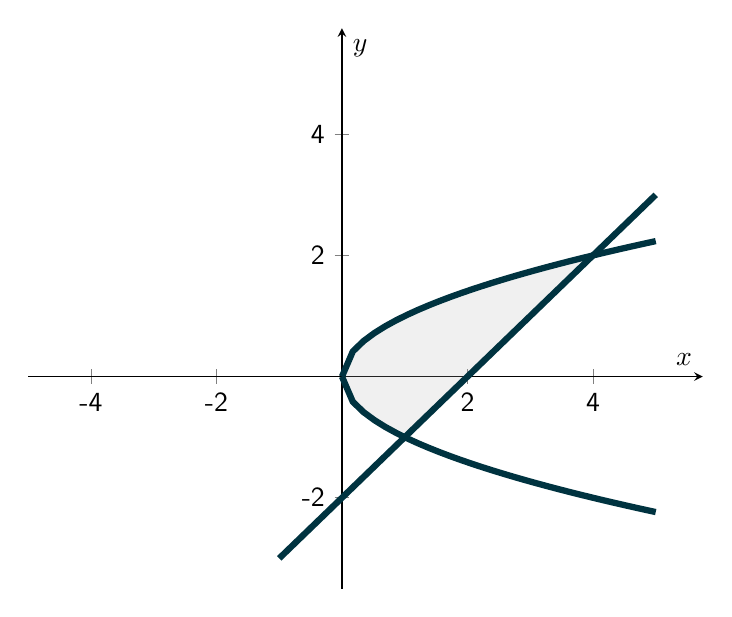
\begin{tikzpicture}[scale=1.25]
            \begin{axis}[
            axis lines = middle, very thick,
            xlabel = {$x$},
            ylabel = {$y$},
            xmin=-5, xmax=5.75,
            ymin=-3.5, ymax=5.75,
            xtick={-4,-2,0,2,4},
            xticklabels={-4,-2,0,2,4},
            ytick={-2,0,2,4},
            yticklabels={-2,0,2,4}        
            ]
            % Curves
            \addplot [name path = A,-,domain = 0:5, line width=0.8mm,DarkBlue,samples = 30] {sqrt(x)} ;
            \addplot [name path = B,-,domain = 0:5, line width=0.8mm,DarkBlue,samples = 30] {-sqrt(x)} ;
            \addplot [name path = C, line width=0.8mm, samples=4, smooth,domain=0:5, DarkBlue] coordinates {(-1,-3)(5,3)};
            % Fill area between paths
            \addplot [black!30, opacity=0.2] fill between [of = A and B, soft clip={domain=0:1}];
            \addplot [black!30, opacity=0.2] fill between [of = A and C, soft clip={domain=1:4}];
            \end{axis}
        \end{tikzpicture}    
    \end{center}   
        
    Thus
    \begin{align}
        \bar y &= \frac{M_x}M = \frac1M \int_{-1}^{2}\int_{y^2}^{y+2} 12y \, dx \, dy
    \end{align} 
    Thus
    \begin{align}
        a &= -1 \\
        b &= 2 \\
        c&= y^2 \\
        d&= y+2 \\
        f(x,y) &= \delta y = 12y
    \end{align}
    }
   \else

   \fi
    
\fi

\ifnum \Version=7
% SHORT SPHERICAL AND CYLINDRICAL EXERCISE
\part Point $P$ has rectangular (Cartesian) coordinates $(x,y,z) = (-6,0,8)$ in $\mathbb R^3$. In cylindrical coordinates, the point is $(r,\theta,z)$, and in spherical coordinates the point is $(\rho, \phi, \theta)$. Where $r=\framebox{\strut\hspace{1cm}}$, $\theta=\framebox{\strut\hspace{2cm}}$, $z=\framebox{\strut\hspace{1cm}}$, $\rho=\framebox{\strut\hspace{2cm}}$, and $\phi=\framebox{\strut\hspace{3cm}}$. 

    \ifnum \Solutions=1 {\color{DarkBlue} \textit{Solutions:} To convert to cylindrical we can use the equation $r^2 = x^2 + y^2$. 
    \begin{align}
        r^2 &= x^2 + y^2 = (-6)^2 + 0^2 = 36 \ \Rightarrow \ r = 6
    \end{align}
    To determine $\theta$ we can use $\tan\theta = y/x$. 
    \begin{align}
        \tan \theta &= \frac{y}{x} = \frac{0}{-6} = 0  \\
        \theta &= \arctan 0 
    \end{align} 
    The point in cylindrical is: 
    \begin{align}
        (r,\theta,z) &= (6,\pi,8) \\
        r &= 6 \\
        \theta &= \pi \\
        z &= 8
    \end{align}
    In spherical, we can start by obtaining $\rho$. 
    \begin{align}
        \rho^2 &= x^2+y^2+z^2\\
        \rho^2 &= (-6)^2 + 0^2 + 8^2 = 36+64 = 100 \\
        \rho &= 10
    \end{align}
    To obtain $\phi$ we can use the equation that relates $x$ to spherical. Using the expression for $x$, and the values that we already have for $x$, $\rho$ and $\theta$:
    \begin{align}
        x &= \rho \sin\phi \cos\theta \\
        -6 &= 10\sin\phi \cos(\pi) \\
        \sin\phi &= \frac{-6}{10 \cos(\pi)}  = \frac{6}{10}\\
        \phi &= \arcsin (6/10)
    \end{align}
    Our coordinates in spherical are
    \begin{align}
        \rho &= 10\\
        \phi &= \arcsin (6/10)\\
        \theta &= \pi
    \end{align}
    Note the following.
    \begin{itemize}
        \item We can, for this exercise, leave un-evaluated trig functions in the answer, because the question didn't specify that you should simplify your answer as much as possible. So it would be ok to leave your answer for $\theta$ as $\arctan 0$ or $\tan^{-1} 0$. 
        \item Our particular textbook uses the convention $(\rho, \phi, \theta)$, not $(\rho, \theta,\phi)$.
    \end{itemize}
    } 
    \else
      
    \fi
    
\fi





\ifnum \Version=8
% SHORT SPHERICAL AND CYLINDRICAL EXERCISE
\part Point $P$ has rectangular (Cartesian) coordinates $(x,y,z) = (4,4,7)$ in $\mathbb R^3$. In cylindrical coordinates, the point is $(r,\theta,z)$, and in spherical coordinates the point is $(\rho, \phi, \theta)$. Where $r=\framebox{\strut\hspace{1cm}}$, $\theta=\framebox{\strut\hspace{2cm}}$, $z=\framebox{\strut\hspace{1cm}}$, $\rho=\framebox{\strut\hspace{2cm}}$, and $\phi=\framebox{\strut\hspace{3cm}}$. 

    \ifnum \Solutions=1 {\color{DarkBlue} \textit{Solutions:} To convert to cylindrical we can use the equation $r^2 = x^2 + y^2$. 
    \begin{align}
        r^2 &= x^2 + y^2 = (4)^2 + 4^2 = 32 \ \Rightarrow \ r = \sqrt{32} = 4\sqrt2
    \end{align}
    It isn't necesssary to simplify to $4\sqrt2$. Then to determine $\theta$ we can use $\tan\theta = y/x$. 
    \begin{align}
        \tan \theta &= \frac{y}{x} = \frac{4}{4} = 1  \\
        \theta &= \arctan \pi/4
    \end{align} 
    The point in cylindrical is: 
    \begin{align}
        (r,\theta,z) &= (4\sqrt2,\pi/4,7) \\
        r &= 4\sqrt2 \\
        \theta &= \pi/4 \\
        z &= 7
    \end{align}
    In spherical, we can start by obtaining $\rho$. 
    \begin{align}
        \rho^2 &= x^2+y^2+z^2\\
        \rho^2 &= (4)^2 + 4^2 + 7^2 = 16+16+49 = 32+49 = 81 \\
        \rho &= 9
    \end{align}
    To obtain $\phi$ we can use the equation that relates $x$ to spherical. Using the expression for $x$, and the values that we already have for $x$, $\rho$ and $\theta$:
    \begin{align}
        x &= \rho \sin\phi \cos\theta \\
        4 &= 9\sin\phi \cos(\pi/4) \\
        \sin\phi &= \frac{4}{9 \cos(\pi/4)}  = \frac{4\sqrt2}{9}\\
        \phi &= \arcsin \left(\frac{4\sqrt2}{9}\right)
    \end{align}
    Note for $\phi$ we can also use:
    \begin{align}
        y &= \rho \sin\phi \sin\theta \\
        4 &= 9\sin\phi \sin(\pi/4) \\
        \sin\phi &= \frac{4}{9 \sin(\pi/4)}  = \frac{4\sqrt2}{9}\\
        \phi &= \arcsin \left(\frac{4\sqrt2}{9}\right)
    \end{align}    
    And we can also use:
    \begin{align}
        z &= \rho \cos\phi  \\
        7 &= 9\cos\phi  \\
        \sin\phi &= \frac{4}{9 \sin(\pi/4)}  = \frac{4\sqrt2}{9}\\
        \phi &= \arccos \left(\frac{7}{9}\right)
    \end{align}      
    Our coordinates in spherical are
    \begin{align}
        \rho &= 9\\
        \phi &= \arcsin \left(\frac{4\sqrt2}{9}\right), \ \textbf{or} \ \phi = \arccos(7/9)\\
        \theta &= \pi/4
    \end{align}
    Note the following.
    \begin{itemize}
        \item We can, for this exercise, leave un-evaluated trig functions in the answer, because the question didn't specify that you should simplify your answer as much as possible. So it would be ok to leave your answer for $\theta$ as $\arctan 1$ or $\tan^{-1} 1$. 
        \item Our particular textbook uses the convention $(\rho, \phi, \theta)$, not $(\rho, \theta,\phi)$.
    \end{itemize}
    } 
    \else
      
    \fi
    
\fi





% 15.6
% CENTROID Y-COORDINATE PARABOLA AND LINE
\ifnum \Version=9
    \part A thin plate with density $\delta=12$ is bounded in the $xy-$plane by $y=3-x^2$ and $y=1-x$. The plate has mass $M$. The $y-$coordinate of the centroid is $\bar y = M_x/M$, where $\displaystyle M_x = \int_A^B \int_C^D f(x,y) \, dy \, dx$,  and $A=\framebox{\strut\hspace{1cm}}$, $B=\framebox{\strut\hspace{1cm}}$, $C=\framebox{\strut\hspace{3cm}}$, $D=\framebox{\strut\hspace{3cm}}$, and $f(x,y) = \framebox{\strut\hspace{3cm}}$. 
    
    \ifnum \Solutions=1 
    {\color{DarkBlue}
    The region is bounded by 
    $$1-x \le y \le 3-x^2$$
    The given curves intersect when 
    \begin{align}
        1-x &= 3-x^2\\
        0 &= x^2-x-2 \\
        &= (x-2)(x+1)
    \end{align}
    The curves intersect at $x=-1,2$. Using $y=1-x$, the intersection points are $(-1,2)$ and $(2,-1)$. The region is shown below. 
    \begin{center}  
        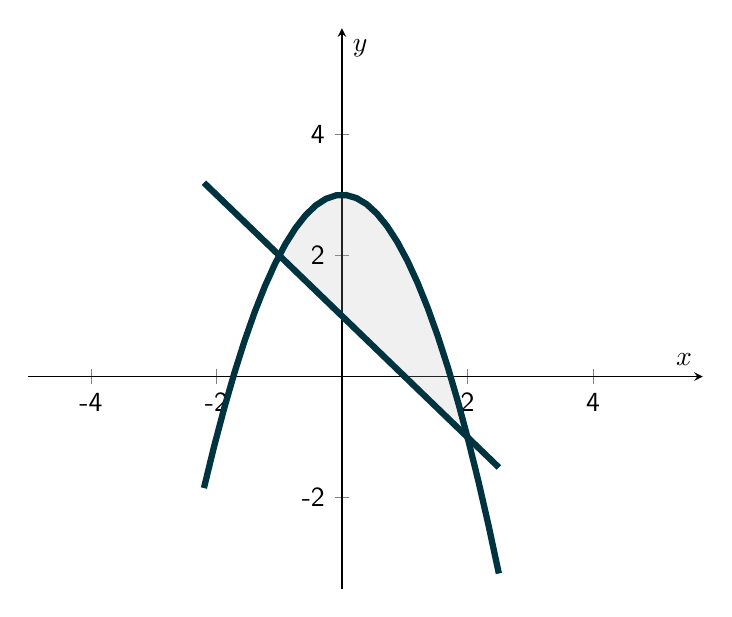
\begin{tikzpicture}[scale=1.25]
            \begin{axis}[
            axis lines = middle, very thick,
            xlabel = {$x$},
            ylabel = {$y$},
            xmin=-5, xmax=5.75,
            ymin=-3.5, ymax=5.75,
            xtick={-4,-2,0,2,4},
            xticklabels={-4,-2,0,2,4},
            ytick={-2,0,2,4},
            yticklabels={-2,0,2,4}        
            ]
            % Curves
            \addplot [name path = A,-,domain = -2.2:2.5, line width=0.8mm,DarkBlue,samples = 30] {3-x^2} ;
            \addplot [name path = C,-,domain = -2.2:2.5, line width=0.8mm,DarkBlue,samples = 4] {1-x} ;
            % Fill area between paths
            \addplot [black!30, opacity=0.2] fill between [of = A and C, soft clip={domain=-1:2}];
            \end{axis}
        \end{tikzpicture}    
    \end{center}   
        
    Thus
    \begin{align}
        \bar y &= \frac{M_x}M = \frac1M \int_{-1}^{2}\int_{1-x}^{3-x^2} 12y \, dy \, dx
    \end{align} 
    Thus
    \begin{align}
        A &= -1 \\
        B &= 2 \\
        C&= 1-x \\
        D&= 3-x^2 \\
        f(x,y) &= \delta y = 12y
    \end{align}
    }
   \else

   \fi
    
\fi
   
    % 13.3 and 13.4
% unit tangent vectors
% arc length
% curvature
% osculating circle
% unit normal

\ifnum \Version=1

\part The unit tangent vector for a curve $\mathbf r(t)$ is $\mathbf T(t) = \langle 0, \cos t, \sin t \rangle$. The unit normal vector is $\mathbf  N = \langle f(t), g(t), g(t) \rangle$, where $f(t) = \framebox{\strut\hspace{2cm}}$, $g(t) = \framebox{\strut\hspace{2cm}}$, $h(t) =\framebox{\strut\hspace{2cm}}$. 

\ifnum \Solutions=1 {\color{DarkBlue} \textit{Answer:} \textit{Solutions:} The normal vector is

\begin{align}
    \mathbf N &= \frac{d\mathbf T/dt}{|d\mathbf T/dt|} 
\end{align}
And
\begin{align}
    \mathbf T'(t) &= \langle 0,-\sin t, \cos t \rangle \\
    |\mathbf T'(t) | &= \sqrt{ 0 +(-\sin t)^2 + (\cos t)^2} =1\\
    \mathbf N &= \frac{d\mathbf T/dt}{|d\mathbf T/dt|} = \langle 0, - \sin(t),  \cos(t) \rangle
\end{align}
} 
\else
\fi        
\fi

\ifnum \Version=2

\part The velocity vector of an object moving on the curve $\mathbf r(t)$ is $\mathbf v(t) = \langle 4\cos (2t), 4\sin (2t) , 3 \rangle$ for $t>0$. The speed of the object for $t>0$ is $s(t) = |\mathbf v | = \framebox{\strut\hspace{1cm}}$. The unit tangent vector for $t>0$ is $\mathbf T = \langle f(t), g(t) , h(t) \rangle$, where $f(t) = \framebox{\strut\hspace{1.5cm}}$, $g(t) = \framebox{\strut\hspace{1.5cm}}$, $h = \framebox{\strut\hspace{1cm}}$. The curvature is $\kappa = \framebox{\strut\hspace{1cm}}$. 

\ifnum \Solutions=1 {\color{DarkBlue} \textit{Answer:} \textit{Solutions:} The speed is the magnitude of the given velocity vector and is
\begin{align}
    s &= |\mathbf v | =  \sqrt{(4\cos2t)^2 + (4\sin2t)^2 + 3^2 } = \sqrt{4^2 (\cos ^2 2 t + \sin^2 2t) + 3^2} = \sqrt{16 + 9} = 5
\end{align}
The unit tangent vector is 
\begin{align}
    \mathbf T &= \frac{\mathbf v}{|\mathbf v|} = \langle \frac{4}{5}\cos(2 t) , \frac 45 \sin (2t), \frac35 \rangle
\end{align}
For curvature we also need
\begin{align}
    \frac{d\mathbf T}{dt } &= \langle -\frac85 \sin 2t, \frac85 \cos 2t,0 \rangle \\
    \left | \frac{d\mathbf T}{dt } \right| &= \sqrt{ \left(-\frac85\sin 2t\right)^2 +   \left(\frac85 \cos 2 t\right)^2 } = \frac85
\end{align}
The curvature is
\begin{align}
    \kappa = \frac{1}{|\mathbf v |}\left| \frac{d\mathbf T}{dt}\right| = \frac{1}{5} \cdot \frac{8}{5} = \frac{8}{25}
\end{align}
} 
\else
\fi        
\fi


\ifnum \Version=3

\part A plane curve $\mathbf r(t)$ has curvature $\kappa = \frac{1}{8}$ at $\mathbf r(t_0) = \langle 15, 2 \rangle$, and the unit normal vector at $t=t_0$ is $\mathbf  N = \mathbf j = \langle 0, 1 \rangle$. The equation of the osculating circle at $t=t_0$ is \framebox{\strut\hspace{3.5cm}}.

\ifnum \Solutions=1 {\color{DarkBlue} \textit{Answer:} \textit{Solutions:} Recall that The circle of curvature, or osculating circle, at a point $P$ on a plane curve where $\kappa \ne 0$ is the circle in the plane of the curve that

\begin{enumerate}
    \item is tangent to the curve at P (has the same tangent line the curve has)
    \item has the same curvature the curve has at P
    \item lies toward the concave or inner side of the curve
\end{enumerate}
The \textbf{radius of curvature} of the curve at P is the radius of the circle of curvature, which is $\frac{1}{\kappa}$. So to obtain the radius, we calculate $\kappa$ and take the reciprocal. The \textbf{center} of the osculating circle of the curve at P lies on the inner side of the curve, and the unit normal points in the direction of the inner side of the planar curve. 

So for this problem we have a circle with radius $1/\kappa = 8$, and whose centre is 8 units away from the point $(15,2)$ in the direction of $\mathbf N$. The circle has equation
$$(x-15)^2 + (y-10)^2 = 8^2$$
} 
\else
  
\fi        
\fi




\ifnum \Version=4

\part The velocity vector for an object moving on the curve $\mathbf r(t)$ is $\mathbf v(t) = \langle t\cos t, t\sin t \rangle$. The speed of the object for $t>0$ is $s(t) = \framebox{\strut\hspace{1cm}}$. The unit tangent vector for $t>0$ is $\mathbf T = \langle f(t), g(t) \rangle$, where $f(t) = \framebox{\strut\hspace{2cm}}$, $g(t) = \framebox{\strut\hspace{2cm}}$. 

\ifnum \Solutions=1 {\color{DarkBlue} \textit{Answer:} \textit{Solutions:} The speed is the magnitude of the velocity vector and is
\begin{align}
    s &= |\mathbf v | = \sqrt{(t\cos t)^2 + (t\sin t)^2 } = \sqrt{t^2 (\cos ^2 t + \sin^2 t)} = |t|
\end{align}
But we are told that $t>0$ so we can use $|t| = t$. The unit tangent vector is 
\begin{align}
    \mathbf T &= \frac{\mathbf v}{|\mathbf v|} = \langle \cos t, \sin t \rangle
\end{align}
} 
\else
\fi        
\fi

\ifnum \Version=5

\part A plane curve $\mathbf r(t)$ has curvature $\kappa = \frac{1}{4}$ at the point $\mathbf r(t_0) = 3\mathbf i + 5\mathbf j$, and the unit normal vector at $t_0$ is $\mathbf  N = \mathbf i = \langle1,0\rangle$. The equation of the osculating circle at $t=t_0$ is \framebox{\strut\hspace{3.5cm}}.

\ifnum \Solutions=1 {\color{DarkBlue} \textit{Answer:} \textit{Solutions:} Recall that The circle of curvature, or osculating circle, at a point $P$ on a plane curve where $\kappa \ne 0$ is the circle in the plane of the curve that

\begin{enumerate}
    \item is tangent to the curve at P (has the same tangent line the curve has)
    \item has the same curvature the curve has at P
    \item lies toward the concave or inner side of the curve
\end{enumerate}
The \textbf{radius of curvature} of the curve at P is the radius of the circle of curvature, which is $\frac{1}{\kappa}$. So to obtain the radius, we calculate $\kappa$ and take the reciprocal. The \textbf{center} of the osculating circle of the curve at P lies on the inner side of the curve, and the unit normal points in the direction of the inner side of the planar curve. 

So for this problem we have a circle with radius $1/\kappa = 4$, and whose centre is 4 units away from the point $(3,5)$ in the direction of $\mathbf N$. The circle has equation
$$(x-7)^2 + (y-5)^2 = 4^2$$
} 
\else
  
\fi        
\fi


\ifnum \Version=6

\part The velocity vector for an object moving on the curve $\mathbf r(t)$ is $\mathbf v(t) = \langle 4t\cos t, 4t\sin t \rangle$ for $t>0$. The speed of the object for $t>0$ is $s(t)  = |\mathbf v | = \framebox{\strut\hspace{1cm}}$. The unit tangent vector for $t>0$ is $\mathbf T = \langle f(t), g(t) \rangle$, where $f(t) = \framebox{\strut\hspace{1.5cm}}$, $g(t) = \framebox{\strut\hspace{1.5cm}}$. The curvature is $\kappa = \framebox{\strut\hspace{1cm}}$. 

\ifnum \Solutions=1 {\color{DarkBlue} \textit{Answer:} \textit{Solutions:} The speed is the magnitude of the given velocity vector and is
\begin{align}
    s &= |\mathbf v | =  \sqrt{(4t\cos t)^2 + (4t\sin t)^2 } = \sqrt{4^2t^2 (\cos ^2 t + \sin^2 t)} = 4|t|
\end{align}
But we are told that $t>0$ so we can assume $|t| = t$. The unit tangent vector is 
\begin{align}
    \mathbf T &= \frac{\mathbf v}{|\mathbf v|} = \langle \cos t, \sin t \rangle
\end{align}
We need
\begin{align}
    \frac{d\mathbf T}{dt } &= \langle -\sin t, \cos t \rangle \\
    \left | \frac{d\mathbf T}{dt } \right| &= \sqrt{ (-\sin t)^2 +   \cos^2 t } = 1
\end{align}
The curvature is
\begin{align}
    \kappa = \frac{1}{|\mathbf v |}\left| \frac{d\mathbf T}{dt}\right| = \frac{1}{4t} 
\end{align}
} 
\else
\fi        
\fi



\ifnum \Version=7

\part The velocity vector of an object moving on the curve $\mathbf r(t)$ is $\mathbf v(t) = \langle 3\cos (2t), 3\sin (2t) \rangle$ for $t>0$. The speed of the object for $t>0$ is $s(t) = |\mathbf v | = \framebox{\strut\hspace{1.5cm}}$. The unit tangent vector for $t>0$ is $\mathbf T = \langle f(t), g(t)  \rangle$, where $f(t) = \framebox{\strut\hspace{2cm}}$, and $g(t) = \framebox{\strut\hspace{2cm}}$.  The curvature for $t>0$ is \framebox{\strut\hspace{1.5cm}}. 

\ifnum \Solutions=1 {\color{DarkBlue} \textit{Answer:} \textit{Solutions:} The speed is the magnitude of the given velocity vector and is
\begin{align}
    s &= |\mathbf v | =  \sqrt{(3\cos t)^2 + (3\sin t)^2  } = \sqrt{3^2 (\cos ^2 t + \sin^2 t) + 3^2} = \sqrt{ 9} = 3
\end{align}
The unit tangent vector is 
\begin{align}
    \mathbf T &= \frac{\mathbf v}{|\mathbf v|} 
    = \langle \frac{3}{3}\cos(2 t) , \frac 33 \sin (2t) \rangle 
    = \langle \cos(2 t) ,  \sin (2t) \rangle
\end{align}
For curvature we also need
\begin{align}
    \frac{d\mathbf T}{dt } &= \langle -2 \sin 2t, 2 \cos 2t\rangle \\
    \left | \frac{d\mathbf T}{dt } \right| &= \sqrt{ \left(-2\sin 2t\right)^2 +   \left(2 \cos 2 t\right)^2 } = 2
\end{align}
The curvature is
\begin{align}
    \kappa = \frac{1}{|\mathbf v |}\left| \frac{d\mathbf T}{dt}\right| = \frac{1}{3} \cdot 2 = \frac{2}{3}
\end{align}
} 
\else
\fi        
\fi


\ifnum \Version=8

\part A plane curve $\mathbf r(t)$ has curvature $\kappa = \frac{1}{4}$ at $\mathbf r(t_0) = \langle 5, 3 \rangle$, and the unit normal vector at $t=t_0$ is $\mathbf  N = \mathbf j = \langle 0, 1 \rangle$. The equation of the osculating circle at $t=t_0$ is \framebox{\strut\hspace{3.5cm}}.

\ifnum \Solutions=1 {\color{DarkBlue} \textit{Answer:} \textit{Solutions:} Recall that The circle of curvature, or osculating circle, at a point $P$ on a plane curve where $\kappa \ne 0$ is the circle in the plane of the curve that

\begin{enumerate}
    \item is tangent to the curve at P (has the same tangent line the curve has)
    \item has the same curvature the curve has at P
    \item lies toward the concave or inner side of the curve
\end{enumerate}
The \textbf{radius of curvature} of the curve at P is the radius of the circle of curvature, which is $\frac{1}{\kappa}$. So to obtain the radius, we calculate $\kappa$ and take the reciprocal. The \textbf{center} of the osculating circle of the curve at P lies on the inner side of the curve, and the unit normal points in the direction of the inner side of the planar curve. 

So for this problem we have a circle with radius $1/\kappa = 4$, and whose centre is 4 units away from the point $(5,3)$ in the direction of $\mathbf N$. The circle has equation
$$(x-5)^2 + (y-7)^2 = 4^2$$
} 
\else
  
\fi        
\fi






\ifnum \Version=9

\part The velocity vector of an object moving on the curve $\mathbf r(t)$ is $\mathbf v(t) = \langle t, 3 \rangle$ for $t>0$. The speed of the object at $t=2$ is $s(2) = |\mathbf v(2) | = \framebox{\strut\hspace{1.75cm}}$. The unit tangent vector at $t=2$ is $\mathbf T(2) = \langle c_1 ,c_2  \rangle$, where $c_1 = \framebox{\strut\hspace{1.75cm}}$, $c_2 = \framebox{\strut\hspace{1.75cm}}$. The curvature is $\framebox{\strut\hspace{1.75cm}}$. 

\ifnum \Solutions=1 {\color{DarkBlue} \textit{Answer:} \textit{Solutions:} The speed is the magnitude of the given velocity vector and is
\begin{align}
    s &= |\mathbf v | =  \sqrt{( t)^2 + (3)^2  } = \sqrt{t^2+9}\\
    s(2) &= \sqrt{2^2+9} = \sqrt{13}
\end{align}
We also need the unit tangent vector at $t=2$. 
\begin{align}
    \mathbf T (t) &= \frac{\mathbf v}{|\mathbf v|} = \frac{t\mathbf i + 3\mathbf j}{\sqrt{t^2+9}} \\
    \mathbf T (2) &= \frac{2\mathbf i + 3\mathbf j}{\sqrt{2^2+9}}  
    = \langle \frac{2}{\sqrt{13}} , \frac {3}{\sqrt{13}}  \rangle \\
    c_1 &= \frac{2}{\sqrt{13}}\\
    c_2 &= \frac{3}{\sqrt{13}}
\end{align}
The curvature is zero because the motion is along a straight line. 
\begin{align}
    \kappa = 0
\end{align}
} 
\else
\fi        
\fi

\ifnum \Version=10

\part A plane curve $\mathbf r(t)$ has curvature $\kappa = \frac{1}{10}$ at $\mathbf r(t_0) = \langle 5, 0 \rangle$, and the unit normal vector at $t=t_0$ is $\mathbf  N = \mathbf j = \langle 0, 1 \rangle$. The equation of the osculating circle at $t=t_0$ is \framebox{\strut\hspace{3.5cm}}.

\ifnum \Solutions=1 {\color{DarkBlue} \textit{Answer:} \textit{Solutions:} Recall that The circle of curvature, or osculating circle, at a point $P$ on a plane curve where $\kappa \ne 0$ is the circle in the plane of the curve that

\begin{enumerate}
    \item is tangent to the curve at P (has the same tangent line the curve has)
    \item has the same curvature the curve has at P
    \item lies toward the concave or inner side of the curve
\end{enumerate}
The \textbf{radius of curvature} of the curve at P is the radius of the circle of curvature, which is $\frac{1}{\kappa}$. So to obtain the radius, we calculate $\kappa$ and take the reciprocal. The \textbf{center} of the osculating circle of the curve at P lies on the inner side of the curve, and the unit normal points in the direction of the inner side of the planar curve. 

So for this problem we have a circle with radius $1/\kappa = 10$, and whose centre is 10 units away from the point $(5,0)$ in the direction of $\mathbf N$. The circle has equation
$$(x-5)^2 + (y-10)^2 = 10^2$$
} 
\else
  
\fi        
\fi
   
\end{parts}

\newpage \question[0.25] \ID
% CHANGE OF VARIABLE (15.8)
% OR APPLICATION (15.6)
% OR TRIPLE CARTESIAN (15.5) 

\ifnum \Version=1
% CENTROID
% BASED ON THOMAS EXERCISES, 15.6 #1
% SUFFICIENT FOR A PRACTICE EXAM
\question[6] A thin plate of density $\delta(x,y) = 12x$ is bounded by the lines $x = 0, y = x$, and the parabola $y = x^2-6$ in the first quadrant. 
\begin{parts} 
    \part Determine the mass of the plate, $M$. Please show your work. 
    \ifnum \Solutions=1 
    {\color{DarkBlue} \textit{Solutions:}
    Curves intersect when $$x = x^2-6 \quad \Rightarrow \quad 0 = x^2 - x - 6 = (x-3)(x+2)$$
    Or $x=3, -2$. We can ignore $x=-2$ because the region is the first quadrant. Curves intersect at the point $(3,3)$, and 
    \begin{align}
        0 \le y \le 3, \quad y \le x \le \sqrt{y+6}
    \end{align}
    The mass is
    \begin{align}
        M &= \int_0^3 \int_y^{\sqrt{y+6}} \delta \, dx \, dy \\
        &= \int_0^3 \int_y^{\sqrt{y+6}} 12x \, dx \, dy \\
        &= \int_0^3  \left. 6x^2 \right|_{x=y}^{x=\sqrt{y+6}} \, dy \\
        &= \int_0^3 6(y + 6 - y^2) \, dy \\
        &= \int_0^3 6y + 36 - 6y^2 \, dy \\
        &= \left. (3y^2 + 36y - 2y^3 ) \right|_0^3 \, dy \\
        &= 27 + 108 - 54 \\
        &= 81
    \end{align}
    }
    \else 
    \vspace{16cm}
    \fi
    \part Use your results from the previous part to set up an integral that can be used to determine the $x-$coordinate of the center of mass of the plate. You do not need to evaluate your integral. 
    \ifnum \Solutions=1 {\color{DarkBlue} \textit{Solutions:} the $x-$coordinate of the center of mass, $\bar x$, is
    \begin{align}
    \bar x &= \frac{M_y}{M} = \frac{1}{81} \int_0^3 \int_y^{\sqrt{y+6}} 12x^2 \, dx \, dy 
    \end{align}
    } 
    \else
      
    \fi
    \end{parts} 
\fi
    





\ifnum \Version=2
% LONGISH CHANGE OF VARIABLE
% VERBATUM FROM SPRING 2022 QUIZ
% hand written solution only
% SUFFICIENT FOR A PRACTICE EXAM
\question[6] Consider the double integral

$$I=\iint_R \frac{x+2y}{2y-x} dA$$

where $R$ is the parallelogram with vertices $(-3,1), (-1,0), (-1,2), (1,1)$. Our goal is to determine the area of the parallelogram using the transform below. 
$$u=x+2y, \qquad v = -x +2y$$ 
Please show your work for the following. 
\begin{parts} 
    \part Use the given transform to calculate the Jacobian of the transform, $J = \partial x(u,v)/\partial y(u,v)$. 
    \ifnum \Solutions=1 
    \else 
    \vspace{8 cm}
    \fi
    \part Use your results from Part (a) and the given transform to transform the double integral. You do not need to evaluate your integral. 
\end{parts} 

\ifnum \Solutions=1 {\color{DarkBlue} \textit{Solutions:} the integral after the transform is $$\displaystyle \frac14 \int_1^5\int_{-1}^3 \frac uv \, du \, dv$$
A screen capture of a hand-written solution from a previous offer of MATH 2551 is below. 
    \begin{figure}[h]
    \centering
    \includegraphics[width=16cm]{202302/Exam3/Images/ImgE3.OR.06.png}
    \end{figure}  
    
    } 
   \else
      
   \fi
    
\fi

\ifnum \Version=3
% CENTROID
% BASED ON THOMAS EXERCISES, 15.6 #1
% SUFFICIENT FOR A PRACTICE EXAM
\question[6] A thin plate with density $\delta(x,y) = 24y$ is bounded by the lines $x = 0, x=2y$, and the parabola $x=y^2$ in the first quadrant. 
\begin{parts} 
    \part Determine the mass of the plate, $M$. Please show your work. 
    
    \ifnum \Solutions=1 
    {\color{DarkBlue} \textit{Solutions:}
    Curves intersect when $$2y = y^2 \quad \Rightarrow \quad 0 = y^2-2y = y(y-2)$$
    Or $y=0,2$. Curves intersect at the points $(0,0)$, $(4,2)$. 
    The mass is
    \begin{align}
        M = \int_0^4 \int_{x/2}^{\sqrt{x}} \delta \, dy \, dx 
        &= \int_0^4 \int_{x/2}^{\sqrt{x}} 24y \, dy \, dx \\
        &= \int_0^4  \left. 12y^2 \right|_{y=x/2}^{y=\sqrt{x}} \, dx \\
        &= 12 \int_0^4 (x-\frac{x^2}{4}) \, dx \\
        &= 12 \left. (\frac{x^2}{2} - \frac{x^3}{12} ) \right|_0^4 \, dy \\
        &= 12 (\frac{16}{2} - \frac{64}{12}) \\
        &= 96 - 64\\
        &= 32
    \end{align}
    \textbf{An Alternate Solution}\\
    Another way to approach this problem is to use the integration order $dx\,dy$. In this case the double integral becomes
    \begin{align}
        M = \int_0^2 \int_{y^2}^{2y} \delta \, dx \, dy
        &= \int_0^2 \int_{y^2}^{2y} 24y \, dx \, dy \\
        &= 24\int_0^2  \left. yx \right|_{x=y^2}^{x=2y} \, dy \\
        &= 24 \int_0^2 (2y^2 - y^3) \, dy \\
        &= 24 \left. (\frac{2y^3}{3} - \frac{y^4}{4} ) \right|_0^2 \, dy \\
        &= 24 (\frac{16}{3} - \frac{16}{4}) \\
        &= \frac{24\cdot16}{3} - 24\cdot 4 \\
        &= 8\cdot16 - 96 \\
        &= 128 - 96 \\
        &= 32
    \end{align}    
    }
    \else 
    \vspace{14cm}
    \fi
    \part Use your results from the previous part to set up an integral that can be used to determine the $x-$coordinate of the center of mass of the plate. You do not need to evaluate your integral. 
    \ifnum \Solutions=1 {\color{DarkBlue} \textit{Solutions:} the $x-$coordinate of the center of mass, $\bar x$, is
    \begin{align}
    \bar x &= \frac{M_y}{M} = \frac{1}{32} \int_0^4 \int_{x/2}^{\sqrt{x}} 24xy \, dy \, dx
    \end{align}
    \textbf{An Alternate Solution}\\    
    It is also ok to use the integration order $dx\,dy$. In this case the double integral becomes
    \begin{align}
    \bar x &= \frac{M_y}{M} = \frac{1}{32} \int_0^2 \int_{y^2}^{2y} 24xy \, dx \, dy 
    \end{align}
    } 
    \else
      
    \fi
    \end{parts} 
\fi

\ifnum \Version=4
% VERSION B
% LONG CHANGE OF VARIABLE
% BASED ON AN EXAMPLE FROM THOMAS
% SECTION 15.8 FROM THOMAS
\question[6] Consider the double integral

$$I= 9 \iint_R (y-2x)^2 \sqrt{x+y} \, dA$$

where $R$ is the region in the first quadrant bounded by the lines $x=0$, $y=0$, and $y=1-x$. Our goal is to determine the area of $R$ using the transform below. 
$$u=x+y, \qquad v = y-2x$$ 
Please show your work for the following. 
\begin{parts} 
    \part Use the given transform to calculate the Jacobian of the transform, $J = \partial x(u,v)/\partial y(u,v)$. 
    \ifnum \Solutions=1 {\color{DarkBlue} \textit{Solutions:} Solving for $x$ and $y$ using an augmented matrix,
    \begin{align}
        \begin{pmatrix} 1 & 1 & u \\-2 & 1 & v\end{pmatrix} 
        \sim \begin{pmatrix} 1 & 1 & u \\0 & 3 & 2u+v\end{pmatrix} 
        \sim \begin{pmatrix} 1 & 0 & u/3 - v/3 \\0 & 1 & 2u/3+v/3 \end{pmatrix} 
    \end{align}
    Thus
    \begin{align}
        x &= \frac13(u-v), \ y = \frac13(2u+v) \\
        J(u,v) & = \begin{vmatrix} \DXDU & \DXDV \\[8pt] \DYDU & \DYDV \end{vmatrix} = \begin{vmatrix} 1/3 & -1/3 \\ 2/3 & 1/3 \end{vmatrix} = 1/9 + 2/9 = 1/3
    \end{align}
    }
    \else 
    \vspace{8 cm}
    \fi
    \part Use the given transform and your results from Part (a) to convert the double integral into a double integral over a region in the $uv-$plane. You do not need to evaluate your integral. 
    \ifnum \Solutions=1 {\color{DarkBlue} \textit{Solutions:} Converting each of the boundaries in the $xy-$plane into the $uv-$plane we obtain
        \begin{align}
            x+y &= 1 \quad \Rightarrow \quad \frac13(u-v) + \frac13(2u+v) = 1 &&\Rightarrow \quad u = 1\\
            x&=0 \quad \Rightarrow \quad \frac13(u-v) = 0 &&\Rightarrow \quad v = u\\
            y&= 0 \quad \Rightarrow \quad \frac13(2u+v) = 0 &&\Rightarrow \quad v = -2u
        \end{align}
        The region is described by either of the following relations:
        \begin{align}
            S_1: & \quad 0 \le u \le 1, \quad -2u \le v \le u \\
            S_2: & \quad -2 \le v \le 0, \quad -v/2 \le u \le 1, \ \text{and } 0 \le v \le 1, \quad v \le u \le 1
        \end{align}
        The first set of inequalities requires only a single double integral, but it is ok to set up two double integrals. If using $S_1$, we use $dv\,du$ and obtain
        \begin{align}
            I= 9 \iint_R (y-2x)^2 \sqrt{x+y} \, dA = 9 \int_0^1 \int_{-2u}^u v^2u^{1/2} \frac13 \,dv\,du
        \end{align}
        If using $S_2$, we use $du\,dv$ and obtain
        \begin{align}
            I= 9 \iint_R (y-2x)^2 \sqrt{x+y} \, dA 
            = 9 \int_{-2}^0 \int_{-v/2}^1 v^2u^{1/2} \frac13 \,du\,dv
            + 9 \int_{0}^1 \int_{v}^1 v^2u^{1/2} \frac13 \,du\,dv
        \end{align}        
        } 
       \else
          
       \fi
    \end{parts} 

    \fi



\ifnum \Version=5
    % USE FOR VERSION B
    % LONG CYLINDRICAL WITH APPLICATION TO MASS WITH VARYING DENSITY
    % FROM 15.8
    \question[6] An object $D$ lying in the first octant is bounded below by the $xy-$plane, above by the plane $z=3+4y$, and by the cylinder $x^2+y^2 = 4$. The density of the object at any point in $D$ is equal to the distance from the point to the $z$-axis.  Please show your work for the following.
    
    \begin{parts} 
    \part Use cylindrical coordinates to calculate the total of mass of the object, $M$. Please show your work. 
    
    \ifnum \Solutions=1 {\color{DarkBlue} The object is only in the first octant so $$0 \le \theta \le \pi/2$$ Using $\delta = \sqrt{x^2+y^2} = r$, the $z-$coordinate of the center of mass is computed using 
    \begin{align}
        M &= \iiint_D  \delta \, dV \\
        &= \int_0^{\pi/2} \int_0^2 \int_0^{3+4r\sin\theta}  \delta(r,\theta) \, r\, dz\,dr\,d\theta\\
        &= \int_0^{\pi/2} \int_0^2 \int_0^{3+4r\sin\theta}   r^2 \, dz\,dr\,d\theta\\
        &= \int_0^{\pi/2} \int_0^2    r^2 \, (3+4r\sin\theta) \,dr\,d\theta \\
        &= \int_0^{\pi/2} \int_0^2     \, (3r^2+4r^3\sin\theta) \,dr\,d\theta \\
        &= \int_0^{\pi/2}  \left. \, (r^3+r^4\sin\theta) \right|_{r=0}^{r=2} d\theta \\
        &= \int_0^{\pi/2}  (8 + 16\sin\theta) d\theta \\
        &=  \left. (8\theta - 16\cos\theta) \right|_0^{\pi/2} \\
        &=  (4\pi - 0) - (0 - 16) \\
        &= 4\pi + 16
    \end{align}
    
    } 
    \else
        \vspace{14cm}
    \fi
    
    \part Use your results from the previous part to set up a triple integral in cylindrical coordinates that can be used to determine the $z-$coordinate of the center of mass of the object. You do not need to evaluate your integral. 

    \ifnum \Solutions=1 {\color{DarkBlue} \textit{Solutions:} the $z-$coordinate of the center of mass, $\bar x$, is
    \begin{align}
    \bar z &= \frac{M_{xy}}{M} = \frac{1}{16\pi+16} \int_0^{\pi/2} \int_0^2 \int_0^{3+4r\sin\theta}  z \, \delta(r,\theta) \, r\, dz\,dr\,d\theta
    \end{align}
    } 
    \else
      
    \fi
    \end{parts} 
\fi


% TRANSFORM: SOLVE FOR X & Y, BOUNDARIES, EVALUATE, TRIANGLES
% VERSION A
\ifnum \Version=6
    \question[6] Consider the transform $u=x+y$ and $v=4x+5y$, and the integral $\displaystyle I = \iint_{R}  \,dxdy$. Region $R$ is the triangle in the $xy$-plane bounded by $x+y=0$, $4x+5y=0$, $6x+7y=4$. The transform maps $R$ to region $G$ in the $uv-$plane.  Please show your work for the following.

    \begin{enumerate}
        \item[a)] Solve the system, $u=x+y$ and $v=4x+5y$, for $x$ and $y$ in terms of $u$ and $v$.
            \ifnum \Solutions=1 {\color{DarkBlue} \\[12pt] 
            \textbf{Solutions:}
            We can use the expressions for $u$ and $v$ as an augmented matrix and row reduce. 
            \begin{align}
                \begin{pmatrix} 1 & 1 & u \\ 4 & 5 & v\end{pmatrix} 
                \sim \begin{pmatrix} 1 & 1 & u \\0 & 1 & v - 4u \end{pmatrix} 
                \sim \begin{pmatrix} 1 & 0 & 5u - v \\ 0 & 1 & v - 4u \end{pmatrix} 
            \end{align}
            Thus $x = 5u - v$, and $y = v - 4u$. 
            } 
            \else 
            \vspace{5cm}
            \fi
        \item[b)] Transform the boundaries of $R$ to the $uv-$plane. In other words, determine the boundaries of $G$ in terms of $u$ and $v$. 
            \ifnum \Solutions=1 {\color{DarkBlue} \\[12pt] 
            \textbf{Solutions:} the three lines are transformed below. 
            \begin{itemize}
                \item The line $x+y=0$ becomes $u=0$. 
                \item The line $4x+5y=0$ becomes $v=0$. 
                \item The line $6x+7y=4$ is: 
                \begin{align}
                    6x+7y &=4 \\
                    6\cdot(5u-v) + 7\cdot(v-4u) &= 4\\
                    30u -28u -6v+7v &=4 \\
                    v &= 4 -2u
                \end{align}
            \end{itemize}
            } 
        \else 
        \vspace{5cm}
        \fi        
            
        \item[c)] Use the given transformation and your results from parts (a) and (b) to set up a double integral that in the $uv-$plane that is equal to $I$. Do not evaluate the integral. You also do not need to calculate the Jacobian and may use that the Jacobian of the transform is $J(u,v) = 1$.
            \ifnum \Solutions=1 {\color{DarkBlue} \\[12pt] 
            \textbf{Solutions:}
            \begin{align}
                \iint_{R} \,dx\,dy
                &= \iint_{G}  \left| J(u,v) \right| \,dv\,du 
                = \int_0^2\int_{0}^{4-2u}  \left| 1 \right| \,dv\,du 
                = \int_0^2\int_{0}^{4-2u} \,dv\,du
            \end{align}
            Note the following.
            \begin{itemize}
                \item We did not need to compute the Jacobian but it is computed as follows. 
                $$J 
                = \begin{vmatrix} x_u & x_v \\ y_u & y_v \end{vmatrix} 
                = \begin{vmatrix} 5 & -1 \\ -4 & 1\end{vmatrix} 
                = 5 - 4
                = 1$$
                \item             We did not need to evaluate the integral but if we did:
            \begin{align}
                I = \int_0^2\int_{0}^{4-2u}  \left| 1 \right| \,dv\,du
                = 1 \int_0^2 (4-2u) \,du
                =  \left. 4u - u^2 \right|_0^2 
                = 4
            \end{align}
            \item It is also ok to use the other integration order: $I = \int_0^4\int_0^{2-v/2} \, du \, dv$.
            \end{itemize}
            } 
            \else 
            \fi        
    \end{enumerate}
 
\fi 



% TRANSFORM: SOLVE FOR X & Y, BOUNDARIES, EVALUATE, PARALLELOGRAM
% VERSION A
\ifnum \Version=7
    \question[6] Consider the integral $\displaystyle I = 2\iint_{R} x-4y \,dx\,dy$, where $R$ is the parallelogram in the $xy$-plane bounded by $x-4y=2$, $x-4y=1$, $3y-x=3$, $3y-x=6$. Suppose the transform $u=x-4y$ and $v=3y-x$, maps region $R$ to region $G$ in the $uv-$plane.  Please show your work for the following.

    \begin{enumerate}
        \item[a)] Solve the system, $u=x-4y$ and $v=3y-x$, for $x$ and $y$ in terms of $u$ and $v$.
            \ifnum \Solutions=1 {\color{DarkBlue} \\[12pt] 
            \textbf{Solutions:}
            We can use the expressions for $u$ and $v$ as an augmented matrix and row reduce. 
            \begin{align}
                \begin{pmatrix} 1 & -4 & u \\ -1 & 3 & v\end{pmatrix} 
                \sim \begin{pmatrix} 1 & -4 & u \\0 & -1 & v + u\end{pmatrix} 
                \sim \begin{pmatrix} 1 & 0 & -3u-4v\\0 & 1 & -u-v\end{pmatrix} 
            \end{align}
            Thus
            \begin{align}
                x &=  -3u-4v\\
                y &= -u-v
            \end{align}

            } 
            \else 
            \vspace{5cm}
            \fi
        \item[b)] Transform the boundaries of $R$ to the $uv-$plane. In other words, determine the boundaries of $G$ in terms of $u$ and $v$. 
            \ifnum \Solutions=1 {\color{DarkBlue} \\[12pt] 
            \textbf{Solutions:} the four lines are transformed below. 
            \begin{itemize}
                \item The line $x-4y=2$ becomes $u=2$. 
                \item The line $x-4y=1$ becomes $u=1$. 
                \item The line $3y-x=3$ becomes $v=3$. 
                \item The line $3y-x=6$ becomes $v=6$. 
            \end{itemize}
            } 
        \else 
        \vspace{5cm}
        \fi        
            
        \item[c)] Use the given transformation and your results from parts (a) and (b) to set up a double integral that in the $uv-$plane that is equal to $I$. Do not evaluate the integral. You also do not need to calculate the Jacobian and may use that the Jacobian of the transform is  $J(u,v) = -1$. 
            \ifnum \Solutions=1 {\color{DarkBlue} \\[12pt] 
            \textbf{Solutions:}
            \begin{align}
                \iint_{R} 2x-8y \,dx\,dy
                = \iint_{G} 2u \left| J(u,v) \right| \,du\,dv
                = \int_3^6\int_{1}^2 2u \left| -1 \right| \,du\,dv
                = \int_3^6\int_{1}^2 2u \,du\,dv
            \end{align}
            Note the following.
            \begin{itemize}
                \item We did not need to evaluate the integral, but if we did: 
                \begin{align}
                \iint_{R} 2x-8y \,dx\,dy
                &= \iint_{G} 2u \left| J(u,v) \right| \,du\,dv\\
                &= \int_3^6\int_{1}^2 2u \left| -1 \right| \,du\,dv\\
                &= \int_3^6\left. u^2 \right|_{1}^2 \,dv\\
                &= \int_3^6 3 \,dv\\
                &= 3 \cdot(6 -3) \\
                &= 9
            \end{align}
            \end{itemize}
            } 
            \else 
            \fi        
    \end{enumerate}
 
\fi 




% TRANSFORM: SOLVE FOR X & Y, BOUNDARIES, EVALUATE
% VERSION B
\ifnum \Version=8
    \question[6] Consider the transform $u=x-y$ and $v=4y-2x$, and the integral $\displaystyle I = \iint_{R} \,dxdy$, where $R$ denotes the triangle in the $xy$-plane bounded by $x-y=2$, $4y-2x=0$, $3y=2x$. The transform maps region $R$ to region $G$ in the $uv-$plane.  Please show your work for the following.

    \begin{enumerate}
        \item[a)] Solve the system, $u=x-y$ and $v=4y-2x$, for $x$ and $y$ in terms of $u$ and $v$.
            \ifnum \Solutions=1 {\color{DarkBlue} \\[12pt] 
            \textbf{Solutions:}
            We can use the expressions for $u$ and $v$ as an augmented matrix and row reduce. 
            \begin{align}
                \begin{pmatrix} 1 & -1 & u \\ -2 & 4 & v\end{pmatrix} 
                \sim \begin{pmatrix} 1 & -1 & u \\0 & 2 & v + 2u\end{pmatrix} 
                \sim \begin{pmatrix} 1 & -1 & u\\0 & 1 & u+v/2\end{pmatrix} 
                \sim \begin{pmatrix} 1 & 0 & 2u+v/2\\0 & 1 & u+v/2\end{pmatrix} 
            \end{align}
            Thus $x = 2u+v/2$, and $y = u + \frac{v}{2}$. 
            } 
            \else 
            \vspace{5cm}
            \fi
        \item[b)] Transform the boundaries of $R$ to the $uv-$plane. In other words, determine the boundaries of $G$ in terms of $u$ and $v$. 
            \ifnum \Solutions=1 {\color{DarkBlue} \\[12pt] 
            \textbf{Solutions:} the three lines are transformed below. 
            \begin{itemize}
                \item The line $x-y=2$ becomes $u=2$. 
                \item The line $4x-2y=0$ becomes $v=0$. 
                \item The line $3y=2x$ is: 
                \begin{align}
                    3\cdot \left(u+\frac{v}{2}\right) &= 2\cdot \left( 2u+v/2 \right) \\
                    3u + 3v/2 &= 4u + v \\
                    v/2 &= u \\
                    v &= 2u 
                \end{align}
            \end{itemize}
            } 
        \else 
        \vspace{5cm}
        \fi        
            
        \item[c)] Use the given transformation and your results from parts (a) and (b) to set up a double integral that in the $uv-$plane that is equal to $I$. Do not evaluate the integral. You also do not need to calculate the Jacobian and may use that the Jacobian of the transform is  $J(u,v) = \frac12$. 
            \ifnum \Solutions=1 {\color{DarkBlue} \\[12pt] 
            \textbf{Solutions:} the region is
            $$G = \{ (u,v) \in \mathbb R^2 \, | \, 0\le u \le 2, \ 0 \le v \le 2u\}$$
            or we can use
            $$G = \{ (u,v) \in \mathbb R^2 \, | \, 0\le v \le 4, \ v/2 \le u \le 4\}$$ 
            We can write the double integral as:
            \begin{align}
                \iint_{R} \,dx\,dy
                = \iint_{G}  \left| J(u,v) \right| \,dv\,du 
                = \int_0^2\int_{0}^{2u}  \left| \frac12 \right| \,dv\,du
                = \frac12 \int_0^2\int_{0}^{2u} \,dv\,du
            \end{align}
            Note the following.
            \begin{itemize}
                \item We did not need to compute the Jacobian but it is computed as follows. 
                $$J = \begin{vmatrix} x_u & x_v \\ y_u & y_v \end{vmatrix} = \begin{vmatrix} 2 & 1/2 \\ 1 & 1/2\end{vmatrix} = 1 - 1/2 = \frac12$$
                \item We didn't need to evaluate the integral but if we did: 
                \begin{align}
                \iint_{R} \,dx\,dy
                    &= \iint_{G}  \left| J(u,v) \right| \,dv\,du\\
                    &= \int_0^2\int_{0}^{2u}  \left| \frac12 \right| \,dv\,du\\
                    &= \frac12 \int_0^2\left.  v \right|_{v=0}^{v=2u} \,du\\
                    &= \frac12 \int_0^2 2u \,du\\
                    &=  \int_0^2 u \,du\\
                    &= \frac12 \left. u^2\right|_0^2 \\
                    &= 2
            \end{align}                
            \end{itemize}
            } 
            \else 
            \fi        
    \end{enumerate}
 
\fi 









% TRANSFORM: SOLVE FOR X & Y, BOUNDARIES, EVALUATE
% VERSION D 
\ifnum \Version=9
    \question[6] Consider the transform $u=x+y$ and $v=3x+4y$, and the integral $\displaystyle I = \iint_{R} x+y \,dxdy$, where $R$ denotes the triangle in the $xy$-plane bounded by $x+y=0$, $3x+4y=2$, and $2x+3y=0$. The transform maps region $R$ to region $G$ in the $uv-$plane. Please show your work for the following.

    \begin{enumerate}
        \item[a)] Solve the system, $u=x+y$ and $v=3x+4y$, for $x$ and $y$ in terms of $u$ and $v$.
            \ifnum \Solutions=1 {\color{DarkBlue} \\[12pt] 
            \textbf{Solutions:}
            We can use the expressions for $u$ and $v$ as an augmented matrix and row reduce. 
            \begin{align}
                \begin{pmatrix} 1 & 1 & u \\ 3 & 4 & v\end{pmatrix} 
                \sim \begin{pmatrix} 1 & 1 & u \\0 & 1 & v - 3u \end{pmatrix} 
                \sim \begin{pmatrix} 1 & 0 & 4u - v \\ 0 & 1 & v - 3u \end{pmatrix} 
            \end{align}
            Thus $x = 4u - v$, and $y = v - 3u$. 
            } 
            \else 
            \vspace{5cm}
            \fi
        \item[b)] Transform the boundaries of $R$ to the $uv-$plane. In other words, determine the boundaries of $G$ in terms of $u$ and $v$. 
            \ifnum \Solutions=1 {\color{DarkBlue} \\[12pt] 
            \textbf{Solutions:} the three lines are transformed below. 
            \begin{itemize}
                \item The line $x+y=0$ becomes $u=0$. 
                \item The line $3x+4y=2$ becomes $v=2$. 
                \item The line $2x+3y$ is: 
                \begin{align}
                    2x+3y &=0 \\
                    2\cdot(4u-v) + 3\cdot(v-3u) &= 0\\
                    8u -9u  - 2v+3v &=0 \\
                    v &= u
                \end{align}
            \end{itemize}
            } 
        \else 
        \vspace{5cm}
        \fi        
            
        \item[c)] Use the given transformation and your results from parts (a) and (b) to set up a double integral that in the $uv-$plane that is equal to $I$. Do not evaluate the integral. You also do not need to calculate the Jacobian and may use that the Jacobian of the transform is $J(u,v) = 1$. 
            \ifnum \Solutions=1 {\color{DarkBlue} \\[12pt] 
            \textbf{Solutions:}
            \begin{align}
                \iint_{R} x+y \,dx\,dy
                &= \iint_{G} u \left| J(u,v) \right| \,dv\,du\\
                &= \int_0^2\int_{u}^{2} u \left| 1 \right| \,dv\,du\\
                &= \int_0^2\int_{u}^{2} u  \,dv\,du
            \end{align}
            Note the following.
            \begin{itemize}
                \item We could also instead use
                \begin{align}
                    \iint_{R} x+y \,dx\,dy &= \int_0^2\int_{0}^{v} u  \,du\,dv
                \end{align}
                \item We did not need to compute the Jacobian but it is computed as follows. 
                $$J 
                = \begin{vmatrix} x_u & x_v \\ y_u & y_v \end{vmatrix} 
                = \begin{vmatrix} 4 & -1 \\ -3 & 1\end{vmatrix} 
                = 4 - (-1)(-3)
                = 1$$
                \item It wasn't necessary to compute the integral but: 
                \begin{align}
                    \iint_{R} x+y \,dx\,dy
                    &= \iint_{G} u \left| J(u,v) \right| \,dv\,du\\
                    &= \int_0^2\int_{u}^{2} u \left| 1 \right| \,dv\,du\\
                    &= \int_0^2 2u - u^2 \,du\\
                    &= \left. \left( u^2 - \frac{u^3}{3} \right)\right|_0^2 \\
                    &= 4 - 8/3\\
                    &= 4/3
                \end{align}                
            \end{itemize}
            } 
            \else 
            \fi        
    \end{enumerate}
 
\fi 



\newpage \question[0.25] \ID
% SPHERICAL OR CYLINDRICAL (14.7)


\ifnum \Version=1
% READY TO BE USED FOR PRACTICE EXAM
% SPHERICAL INTEGRATION
% VERBATUM FROM SPRING 2022 QUIZ
% OK FOR A PRACTICE EXAM
% hand written solution only
\question[6] Evaluate the triple integral $I=\displaystyle \iiint_D \frac{16\, x}{\sqrt2}  \, dV$, where $D$ is the region in the first octant bounded by $x^2+y^2+z^2=1$ and the planes $y=0$ and $x=y$. Please show your work. Hint: you may need to use the identity $2\sin ^2x = 1 - \cos(2x)$. 

\ifnum \Solutions=1 {\color{DarkBlue} \textit{Solutions:} below is a screen capture of a hand-written solution from a previous offer of MATH 2551. 
    \begin{figure}[h]
    \centering
    \includegraphics[width=16cm]{202302/Exam3/Images/ImgE3.OR.05.png}
    \end{figure}  
    
    } 
   \else
      
   \fi
    
\fi

\ifnum \Version=2
% OK FOR A PRACTICE EXAM
% NOT SO SHORT CYLINDRICAL EXERCISE
% VERBATUM FROM SPRING 2022 QUIZ
% hand written solution only
\question[6] Use cylindrical coordinates to determine the volume of the region bounded above by $z = 4-3x^2-3y^2$ and bounded below by $z = \sqrt{x^2+y^2}$. Please show your work. 

\ifnum \Solutions=1 {\color{DarkBlue} \textit{Solutions:} below is a screen capture of a hand-written solution from a previous offer of MATH 2551. 
    \begin{figure}[h]
    \centering
    \includegraphics[width=11cm]{202302/Exam3/Images/ImgE3.OR1C.png}
    \end{figure}  
    
    There are other ways to set up this particular integral, but the above is sufficient. 

    } 
   \else
      
   \fi
    
\fi






\ifnum \Version=3
% USE FOR VERSION A
% LONG SPHERICAL WITH APPLICATION TO MASS WITH VARYING DENSITY
% FROM 15.8
\question[6] An object $D$ lying in the first octant is bounded by the planes $x=0, y=0, z=0$, and the sphere $x^2+y^2 + z^2 = 4$. The density of the object at any point in $D$ is equal to the distance from the point to the origin. 

\begin{parts}
    \part Use spherical coordinates to calculate the mass of the object, $M$. Please show your work. 
    
    \ifnum \Solutions=1 {\color{DarkBlue} Using $\delta = \sqrt{x^2+y^2+z^2} = \rho$, the mass is computed using 
    \begin{align}
        M &= \int_0^{\pi/2} \int_0^{\pi/2} \int_0^2 \delta \, \rho^2\sin\phi \, d\rho\,d\phi\,d\theta \\
        &= \int_0^{\pi/2} \int_0^{\pi/2} \int_0^2 \rho^3\sin\phi \, d\rho\,d\phi\,d\theta \\
        &= \int_0^{\pi/2} \int_0^{\pi/2} \left. \frac14 \rho^4\sin\phi \right|_0^2 \, d\phi\,d\theta \\
        &= 4 \int_0^{\pi/2} \int_0^{\pi/2} \sin\phi \, d\phi\,d\theta \\
        &= 4 \int_0^{\pi/2} \left. -\cos\phi \right|_0^{\pi/2} \, d\theta \\
        &= 4 \int_0^{\pi/2}  \, d\theta \\
        &= 2\pi
    \end{align}
    
    } 
   \else
      \vspace{14cm}
   \fi    

   \part Use your results from the previous part to set up an integral in spherical coordinates that can be used to determine the $x-$coordinate of the center of mass of the object. You do not need to evaluate your integral. 
    \ifnum \Solutions=1 {\color{DarkBlue} In spherical coordinates, $$x = \rho \sin\phi \cos\theta$$and the $x-$coordinate of the center of mass, $\bar x$, is
    \begin{align}
    \bar x &= \frac{M_{yz}}{M} \\ 
    &= \frac{1}{M} \int_0^{\pi/2} \int_0^{\pi/2} \int_0^2 (\rho \sin\phi \cos\theta) \, \delta \, \rho^2\sin\phi \, d\rho\,d\phi\,d\theta \\
    &= \frac{1}{M} \int_0^{\pi/2} \int_0^{\pi/2} \int_0^2 \rho^4\sin^2\phi \cos\theta \, d\rho\,d\phi\,d\theta 
    \end{align}
    } 
    \else
      
    \fi
    \end{parts} 
 
\fi








\ifnum \Version=4
% USE FOR VERSION B
% LONG CYLINDRICAL WITH APPLICATION TO MASS WITH VARYING DENSITY
% FROM 15.8
\question[6] An object $D$ lying in the first octant is bounded by the planes $x=0, y=0, z=0$, $z=3+4x$ and the cylinder $x^2+y^2 = 4$. The density of the object at a point in $D$ is equal to the distance from the point to the $z$-axis. 

    \begin{parts} 
    \part Use cylindrical coordinates to calculate the total of mass of the object, $M$. Please show your work. 


    \ifnum \Solutions=1 {\color{DarkBlue} \textit{Solutions:} using $\delta = \sqrt{x^2+y^2} = r$, the $z-$coordinate of the center of mass is computed using 
    \begin{align}
        M &= \iiint_D  \delta \, dV \\
        &= \int_0^{\pi/2} \int_0^2 \int_0^{3+4r\cos\theta}  \delta(r,\theta) \, r\, dz\,dr\,d\theta\\
        &= \int_0^{\pi/2} \int_0^2 \int_0^{3+4r\cos\theta}   r^2 \, dz\,dr\,d\theta\\
        &= \int_0^{\pi/2} \int_0^2 \int_0^{3+4r\cos\theta}   r^2 \, dz\,dr\,d\theta \\ 
        &= \int_0^{\pi/2} \int_0^2    r^2 \, (3+4r\cos\theta) \,dr\,d\theta \\
        &= \int_0^{\pi/2} \int_0^2     \, (3r^2+4r^3\cos\theta) \,dr\,d\theta \\
        &= \int_0^{\pi/2}  \left. \, (r^3+r^4\cos\theta) \right|_0^2 \, d\theta \\
        &= \int_0^{\pi/2}  (8+16\cos\theta) d\theta \\
        &=  \left. (8\theta+16\sin\theta) \right|_0^{\pi/2} \\
        &= 4\pi + 16  
    \end{align}
    
    } 
   \else
      \vspace{14cm}      
   \fi
    \part Use your results from the previous part to set up a triple integral that can be used to determine the $z-$coordinate of the center of mass of the object. You do not need to evaluate your integral. 

    \ifnum \Solutions=1 {\color{DarkBlue} \textit{Solutions:} the $z-$coordinate of the center of mass, $\bar x$, is
    \begin{align}
    \bar z &= \frac{M_{xy}}{M} \\
    &= \frac{1}{16 +4\pi} \int_0^{\pi/2} \int_0^2 \int_0^{3+4r\cos\theta}  z \, \delta(r,\theta) \, r\, dz\,dr\,d\theta
    \end{align}
    } 
    \else
      
    \fi
    \end{parts} 
    
\fi


\ifnum \Version=5
% USE FOR VERSION C
% LONG SPHERICAL WITH APPLICATION TO MASS WITH VARYING DENSITY
% FROM 15.8
\question[6] An object $D$ lies above the $xy-$plane and below the upper half of the sphere $x^2+y^2 + z^2 = 4$. The density of the object at any point in $D$ is equal to the distance from the point to the origin. 

\begin{parts}
    \part Use spherical coordinates to calculate the mass of the object, $M$. Please show your work. 
    
    \ifnum \Solutions=1 {\color{DarkBlue} Using $\delta = \sqrt{x^2+y^2+z^2} = \rho$, the mass is computed using 
    \begin{align}
        M &= \int_0^{2\pi} \int_0^{\pi/2} \int_0^2 \delta \, \rho^2\sin\phi \, d\rho\,d\phi\,d\theta \\
        &= \int_0^{2\pi} \int_0^{\pi/2} \int_0^2 \rho^3\sin\phi \, d\rho\,d\phi\,d\theta \\
        &= \int_0^{2\pi} \int_0^{\pi/2} \left. \frac14 \rho^4\sin\phi \right|_0^2 \, d\phi\,d\theta \\
        &= 4 \int_0^{2\pi} \int_0^{\pi/2} \sin\phi \, d\phi\,d\theta \\
        &= 4 \int_0^{2\pi} \left. -\cos\phi \right|_0^{\pi/2} \, d\theta \\
        &= 4 \int_0^{2\pi}  \, d\theta \\
        &= 8\pi
    \end{align}
    
    } 
   \else
      \vspace{14cm}
   \fi    

   \part Use your results from the previous part to set up an integral in spherical coordinates that can be used to determine the $x-$coordinate of the center of mass of the object. You do not need to evaluate your integral. 
   
    \ifnum \Solutions=1 {\color{DarkBlue} In spherical coordinates, $$x = \rho \sin\phi \cos\theta$$and the $x-$coordinate of the center of mass, $\bar x$, is
    \begin{align}
    \bar x &= \frac{M_{yz}}{M} \\ 
    &= \frac{1}{M} \int_0^{2\pi} \int_0^{\pi/2} \int_0^2 (\rho \sin\phi \cos\theta) \, \delta \, \rho^2\sin\phi \, d\rho\,d\phi\,d\theta \\
    &= \frac{1}{M} \int_0^{2\pi} \int_0^{\pi/2} \int_0^2 \rho^4\sin^2\phi \cos\theta \, d\rho\,d\phi\,d\theta 
    \end{align}
    } 
    \else
      
    \fi
    \end{parts} 

 \fi 




\ifnum \Version=6
% USE FOR VERSION B
% LONG CYLINDRICAL WITH APPLICATION TO MASS WITH VARYING DENSITY
% FROM 15.8
\question[6] An object $D$ lying in the first octant is bounded by the planes $y=x, y=0, z=0$, $z=9+8y$ and the cylinder $x^2+y^2 = 1$. The density of the object at any point in $D$ is equal to the distance from the given point to the $z$-axis. 

    \begin{parts} 
    \part Use cylindrical coordinates to calculate the total of mass of the object, $M$. Please show your work. 


    \ifnum \Solutions=1 {\color{DarkBlue} \textit{Solutions:} using $\delta = \sqrt{x^2+y^2} = r$, mass is computed using the following. 
    \begin{align}
        M &= \iiint_D  \delta \, dV \\
        &= \int_0^{\pi/4} \int_0^1 \int_0^{9+8r\sin\theta}  \delta(r,\theta) \, r\, dz\,dr\,d\theta\\
        &= \int_0^{\pi/4} \int_0^1 \int_0^{9+8r\sin\theta}   r^2 \, dz\,dr\,d\theta\\
        &= \int_0^{\pi/4} \int_0^1    r^2 \, (9+8r\sin\theta) \,dr\,d\theta \\
        &= \int_0^{\pi/4} \int_0^1     \, (9r^2+8r^3\sin\theta) \,dr\,d\theta \\
        &= \int_0^{\pi/4}  \left. \, (3r^3+2r^4\sin\theta) \right|_0^1 \, d\theta \\
        &= \int_0^{\pi/4}  (3+2\sin\theta) d\theta \\
        &=  \left. (3\theta-2\cos\theta) \right|_0^{\pi/4} \\
        &= 3\pi/4 - 2/\sqrt2  + 2
    \end{align}
    
    Note the following. 
    \begin{itemize}
        \item We could also write final answer as $M = 3\pi/4 + 2 - \sqrt2$. 
        \item We cannot use:
        \begin{align}
            M = \iiint_D  \delta \, dV 
        &= \int_0^{\pi/4}  \int_0^{9+8r\sin\theta} \int_0^1 r^2\, dr\,dz\,d\theta
        \end{align}
        In other words we can't switch the order of the innermost two integrals because the limits for $z$ use both $r$ and $\theta$. 
        \item A common error might be to use $0 \le \theta \le \pi/2$, which would give us the answer $$M = 3\pi/2 + 2 $$
        The above is not correct!         
        \item A common mistake might be to integrate with respect to the wrong variable. For example, doing something like: 
        \begin{align}
            \int_0^{\pi/4}  (3+2\sin\theta) d\theta 
            &=  \left. (3r+2\sin\theta) \right|_0^{\pi/4} 
        \end{align}     
        The above is not correct! 
    \end{itemize}
    } 
   \else
      \vspace{14cm}      
   \fi
    \part Use your results from the previous part to set up a triple integral that can be used to determine the $z-$coordinate of the center of mass of the object. You do not need to evaluate your integral. 

    \ifnum \Solutions=1 {\color{DarkBlue} \textit{Solutions:} the $z-$coordinate of the center of mass, $\bar z$, is
    \begin{align}
    \bar z 
    &= \frac{M_{xy}}{M} 
    = \frac{1}{M} \int_0^{\pi/4} \int_0^1 \int_0^{9+8r\sin\theta}  z \,  r^2\, dz\,dr\,d\theta
    \end{align}
    Note the following. 
    \begin{itemize}
        \item The limits of integration in part (b) should be identical to what was used in part (a). So if an error were made in the limits for part (a), then points should be deducted in part a. And if the limits in part (b) are the same as what were used in part (a) then no further point deductions are needed for the limits of integration. 
        \item It isn't necessary to re-state what $M$ is in this last part of the question, because it should have been found in part (a). 
    \end{itemize}    
    } 
    \else
      
    \fi
    \end{parts} 
    
\fi



\ifnum \Version=7
% USE FOR VERSION C
% LONG SPHERICAL WITH APPLICATION TO MASS WITH VARYING DENSITY
% FROM 15.8
\question[6] An object $D$ is in the shape of an ice cream cone, as it is bounded on top by the sphere $\rho =2$ and on the sides by the cone $\phi = \pi/4$. The density of the object at any point in $D$ is equal to the distance from the given point to the origin. 

\begin{parts}
    \part Use spherical coordinates to calculate the mass of the object, $M$. Please show your work. 
    
    \ifnum \Solutions=1 {\color{DarkBlue} Using $\delta = \sqrt{x^2+y^2+z^2} = \rho$, the mass is computed using 
    \begin{align}
        M &= \int_0^{2\pi} \int_0^{\pi/4} \int_0^2 \delta \, \rho^2\sin\phi \, d\rho\,d\phi\,d\theta \\
        &= \int_0^{2\pi} \int_0^{\pi/4} \int_0^2 \rho^3\sin\phi \, d\rho\,d\phi\,d\theta \\
        &= \int_0^{2\pi} \int_0^{\pi/4} \left. \frac14 \rho^4\sin\phi \right|_{\rho = 0}^{\rho = 2} \, d\phi\,d\theta \\
        &= 4 \int_0^{2\pi} \int_0^{\pi/4} \sin\phi \, d\phi\,d\theta \\
        &= 4 \int_0^{2\pi} \left. -\cos\phi \right|_0^{\pi/4} \, d\theta \\
        &= -4 \int_0^{2\pi}  \sqrt{2}/2 - 1\, d\theta \\
        &= 8\pi(1-\sqrt2/2)
    \end{align}
    % If we had used $\delta = \rho$ and $\pi/4 \le \rho \le 2$ and $0 \le \phi \le \pi/2$, we would find that 
    % \begin{align}
    %     M &= \int_0^{2\pi} \int_0^{\pi/4} \int_{\pi/4}^2 \rho \, \rho^2\sin\phi \, d\rho\,d\phi\,d\theta \\
    %     = 
    % \end{align}
    } 
   \else
      \vspace{14cm}
   \fi    

   \part Use your results from the previous part to set up an integral in spherical coordinates that can be used to determine the $z-$coordinate of the center of mass of the object. You do not need to evaluate your integral. 
   
    \ifnum \Solutions=1 {\color{DarkBlue} In spherical coordinates, $z = \rho \cos\phi$, and the $z-$coordinate of the center of mass, $\bar z$, is
    \begin{align}
    \bar z &= \frac{M_{xy}}{M} \\ 
    &= \frac{1}{M} \int_0^{2\pi} \int_0^{\pi/4} \int_0^2 (\rho \cos\phi) \, \delta \, \rho^2\sin\phi \, d\rho\,d\phi\,d\theta \\
    &= \frac{1}{M} \int_0^{2\pi} \int_0^{\pi/4} \int_0^2 \rho^4\sin\phi\cos\phi \cos\theta \, d\rho\,d\phi\,d\theta 
    \end{align}
    } 
    \else
      
    \fi
    \end{parts} 

\fi 



\ifnum \Version=8
% LONG CYLINDRICAL WITH APPLICATION TO MASS WITH VARYING DENSITY
% FROM 15.8
% MESSY ALGEBRA BUT CAN BE MADE A BIT EASIER
\question[6] An object $D$ is the right circular cylinder whose base is the cylinder $r=2\cos\theta$ in the $xy-$plane and whose top is the plane $z=15+4y$. The density of the object at any point in $D$ is equal to the distance from the given point to the $z$-axis. 

    \begin{parts} 
    \part Use cylindrical coordinates to calculate the total of mass of the object, $M$. Please show your work. 


    \ifnum \Solutions=1 {\color{DarkBlue} \textit{Solutions:} using $\delta = \sqrt{x^2+y^2} = r$, the total mass is 
    \begin{align}
        M = \iiint_D  \delta \, dV 
        &= \int_{-\pi/2}^{\pi/2} \int_0^{2\cos\theta} \int_0^{15+4r\sin\theta}   r^2 \, dz\,dr\,d\theta\\
        &= \int_{-\pi/2}^{\pi/2} \int_0^{2\cos\theta}    r^2 \, (15+4r\sin\theta) \,dr\,d\theta \\
        &= \int_{-\pi/2}^{\pi/2} \int_0^{2\cos\theta}     \, (15r^2 + 4r^3\sin\theta) \,dr\,d\theta \\
        &= \int_{-\pi/2}^{\pi/2}  \left. \, (5r^3+r^4\sin\theta) \right|_0^{2\cos\theta} \, d\theta \\
        &= \int_{-\pi/2}^{\pi/2}  (40\cos^3\theta+16\cos^4\theta \sin\theta) d\theta \\
        &= 40 \int_{-\pi/2}^{\pi/2}  \cos^3\theta \, d\theta +16 \int_{-\pi/2}^{\pi/2}\cos^4\theta \sin\theta d\theta \label{ref:cos4sin}\\
        &= 80 \int_{0}^{\pi/2}  \cos\theta(1 - \sin^2\theta ) \, d\theta  -\frac{16}{5}\cos^5\theta |_{-\pi/2}^{\pi/2} \\
\        &= 80 \int_{0}^{\pi/2}  \cos\theta \, d\theta - 80\int_{0}^{\pi/2} \cos\theta \sin^2\theta \, d\theta  + 0 \\
        &= 80  \sin\theta \huge|_{0}^{\pi/2} - \frac{80}{3} \sin^3\theta|_{0}^{\pi/2} \\
        &= 80  - \frac{80}{3} 
    \end{align}    
    Note that the second term in (\ref{ref:cos4sin}) is the integral of an odd function over a symmetric integral, so it must be zero. Also in (\ref{ref:cos4sin}) we used the idea that integrals of even functions over symmetric intervals centered on the origin can be simplified. 
    } 
   \else
      \vspace{14cm}      
   \fi
    \part Use your results from the previous part to set up a triple integral that can be used to determine the $z-$coordinate of the center of mass of the object. You do not need to evaluate your integral. 

    \ifnum \Solutions=1 {\color{DarkBlue} \textit{Solutions:} the $z-$coordinate of the center of mass, $\bar z$, is
    \begin{align}
    \bar z &= \frac{M_{xy}}{M} 
    = \frac{1}{M} \int_{-\pi/2}^{\pi/2} \int_0^{2\cos\theta} \int_0^{15+4r\sin\theta}  z \,  r^2\, dz\,dr\,d\theta
    \end{align}
    } 
    \else
      
    \fi
    \end{parts} 
    
\fi





\ifnum \Version=9
% LONG CYLINDRICAL WITH APPLICATION TO MASS WITH VARYING DENSITY
% FROM 15.8
% MESSY ALGEBRA BUT CAN BE MADE A BIT EASIER
\question[6] An object $D$ is the right circular cylinder whose base is the cylinder $r=2\cos\theta$ in the $xy-$plane and whose top is the plane $z=15+4y$. The density of the object at any point in $D$ is equal to the distance from the given point to the $z$-axis. 

    \begin{parts} 
    \part Use cylindrical coordinates to calculate the total of mass of the object, $M$. Please show your work. 


    \ifnum \Solutions=1 {\color{DarkBlue} \textit{Solutions:} using $\delta = \sqrt{x^2+y^2} = r$, the total mass is 
    \begin{align}
        M &= \iiint_D  \delta \, dV \\
        &= \int_{-\pi/2}^{\pi/2} \int_0^{2\cos\theta} \int_0^{15+4r\sin\theta}  \delta(r,\theta) \, r\, dz\,dr\,d\theta\\
        &= \int_{-\pi/2}^{\pi/2} \int_0^{2\cos\theta} \int_0^{15+4r\sin\theta}   r^2 \, dz\,dr\,d\theta\\
        &= \int_{-\pi/2}^{\pi/2} \int_0^{2\cos\theta}    r^2 \, (15+4r\sin\theta) \,dr\,d\theta \\
        &= \int_{-\pi/2}^{\pi/2} \int_0^{2\cos\theta}     \, (15r^2 + 4r^3\sin\theta) \,dr\,d\theta \\
        &= \int_{-\pi/2}^{\pi/2}  \left. \, (5r^3+r^4\sin\theta) \right|_0^{2\cos\theta} \, d\theta \\
        &= \int_{-\pi/2}^{\pi/2}  (40\cos^3\theta+16\cos^4\theta \sin\theta) d\theta \\
        &= 40 \int_{-\pi/2}^{\pi/2}  \cos^3\theta \, d\theta +16 \int_{-\pi/2}^{\pi/2}\cos^4\theta \sin\theta d\theta 
    \end{align}
    The second term is the integral of an odd function over a symmetric integral, so it must be zero. The first term is the integral of an even function over a symmetric interval, so it can be simplified.
    \begin{align}
        M 
        &= 80 \int_{0}^{\pi/2}  \cos^3\theta \, d\theta  \\
        &= 80 \int_{0}^{\pi/2}  \cos\theta(1 - 
        \sin^2\theta ) \, d\theta  \\
        &= 80 \int_{0}^{\pi/2}  \cos\theta \, d\theta - 80\int_{0}^{\pi/2} \cos\theta \sin^2\theta \, d\theta  \\
        &= 80  \sin\theta \huge|_{0}^{\pi/2} - \frac{80}{3} \sin^3\theta|_{0}^{\pi/2} \\
        &= 80  - \frac{80}{3} 
    \end{align}    

    } 
   \else
      \vspace{14cm}      
   \fi
    \part Use your results from the previous part to set up a triple integral that can be used to determine the $z-$coordinate of the center of mass of the object. You do not need to evaluate your integral. 

    \ifnum \Solutions=1 {\color{DarkBlue} \textit{Solutions:} the $z-$coordinate of the center of mass, $\bar z$, is
    \begin{align}
    \bar z &= \frac{M_{xy}}{M} 
    = \frac{1}{M} \int_{-\pi/2}^{\pi/2} \int_0^{2\cos\theta} \int_0^{15+4r\sin\theta}  z \,  r^2\, dz\,dr\,d\theta
    \end{align}
    } 
    \else
      
    \fi
    \end{parts} 
    
\fi





\ifnum \Version=12
% LONG CYLINDRICAL THAT USES MOMENT OF INERTIA
% VERBATUM FROM SPRING 2022 QUIZ
% hand written solution only
\question[6] An object $D$ is bounded by the planes $z=0$ and $z=3+4x+8y$ and the cylinder $x^2+y^2 = 2$. The density of the object at a point is equal to the distance from the point to the $z$-axis. Use cylindrical coordinates to calculate the moment of inertia of $D$ about the $z$-axis.

\ifnum \Solutions=1 {\color{DarkBlue} \textit{Solutions:} A screen capture from a hand-written solution from a previous offer of MATH 2551 is below. 
    \begin{figure}[h]
    \centering
    \includegraphics[width=12cm]{2023Spr/Exam3/Images/ImgE3.OR.07.png}
    \end{figure}  
    
    } 
   \else
      
   \fi
    
\fi
    


\end{questions}

% EXAM VERSION D
\newpage 
\renewcommand{\Version}{9} 
% TEST SPECIFIC INFORMATION
\ifnum \Version=1 \renewcommand{\TestName}{Year 1 MATH 2551 Exam 3 Sample A} \fi
\ifnum \Version=2 \renewcommand{\TestName}{Year 1 MATH 2551 Exam 3 Sample B} \fi
\ifnum \Version=3 \renewcommand{\TestName}{Year 1 MATH 2551 Exam 3 Sample C} \fi
\ifnum \Version=4 \renewcommand{\TestName}{Year 1 MATH 2551 Exam 3 Sample D} \fi
\ifnum \Version=5 \renewcommand{\TestName}{Year 1 MATH 2551 Exam 3 Sample E} \fi
\ifnum \Version=6 \renewcommand{\TestName}{Year 1 MATH 2551 Exam 3 Version A} \fi
\ifnum \Version=7 \renewcommand{\TestName}{Year 1 MATH 2551 Exam 3 Version B} \fi
\ifnum \Version=8 \renewcommand{\TestName}{Year 1 MATH 2551 Exam 3 Version C} \fi
\ifnum \Version=9 \renewcommand{\TestName}{Year 1 MATH 2551 Exam 3 Version D} \fi



% TITLE
\begin{center}
\ifnum \Solutions=1 {\Large {\color{DarkBlue}\textit{Solutions}}\\[6pt]}\fi
{\Large \TestName}
\end{center}

\vspace{-16pt}

\begin{center}
\textit{Work done on scratch paper will not be graded.}

\vspace{8pt}
\textbf{A Few Helpful Formulas}
\vspace{8pt}

$
\begin{array}{llllll}
    & \displaystyle x = \rho \sin\phi \cos\theta,
    & \displaystyle y = \rho \sin\phi \sin\theta,
    & \displaystyle z = \rho \cos\phi,
    & \displaystyle dV = \rho^2 \sin \phi \, d\rho \, d\phi \, d\theta,
    & \displaystyle J(u,v) = x_uy_v - y_ux_v
\end{array} 
$
\end{center}
\begin{questions}
\question[0.5] \ID

\question[7] Fill in the blanks. You do not need to show your work. 
    
\begin{parts}
    %SECTIONS 12.1 TO 12.2 (3D, vectors)



\ifnum \Version=1
\part If $P$ is the point $(2, 8, 4)$, then the distance between $P$ and the $xy$-plane is $\framebox{\strut\hspace{1cm}}$ and the distance between $P$ and the $y$-axis is $\framebox{\strut\hspace{1cm}}$. 

\ifnum \Solutions=1 {\color{DarkBlue} \textit{Answer:} the point is 4 units above the $xy$-plane, so the first distance is 4. Looking down the $y$-axis, the point is 2 units to the left of the $y$-axis and 8 units above it, so using a right-angle triangle and the Pythgorean theorem the point is $\sqrt{2^2 + 4^2} = \sqrt{20}$ units away for the $y$-axis. 
} 
\else
  
\fi
\fi


\ifnum \Version=2
\part The point on the sphere $(x-2)^2+(y-4)^2+(z-7)^2=4$ nearest to the $xy-$plane is $P=(a,b,c)$, where $a=\framebox{\strut\hspace{.8cm}}, b=\framebox{\strut\hspace{.8cm}}, c=\framebox{\strut\hspace{.8cm}}$. The radius of the sphere is $r = \framebox{\strut\hspace{.8cm}}$. 

\ifnum \Solutions=1 {\color{DarkBlue} \textit{Answer:} $a=2$, $b=4$, $c=5$, $r = 2$. \\[12pt] \textit{Solutions:} The sphere has center $(2,4,7)$ and radius $r = 2$. Because the radius is 2 and the center has $z$--coordinate $z=7$, the sphere lies above the $xy$-plane. The point on the bottom of the sphere closest to the $xy$-plane will be 2 units directly below the center. The coordinate is $(2,4,5)$, so $a=2$, $b=4$, $c=5$. 

} 
\else
  
\fi
\fi






\ifnum \Version=3
\part An equation of the plane that is perpendicular to the $x$-axis and passes through the point $P(3,4,5)$ is $\framebox{\strut\hspace{4cm}}$. 

\ifnum \Solutions=1 {\color{DarkBlue} \textit{Answer:} The plane has equation 
\begin{align}
    \vec n \cdot (\vec x - \vec x_0) & = 0
\end{align}
Where $\vec n$ is a vector normal to the plane, $\vec x_0$ is any point in the plane, and $\vec x $ is the variable vector. We can use: 
\begin{align}
    \begin{pmatrix} 1\\0 \\0 \end{pmatrix} \cdot \left( \begin{pmatrix} x\\y\\z\end{pmatrix}  - \begin{pmatrix}3\\4\\5 \end{pmatrix} \right) & = 0 \\
    x-3 &=0 \\
    x&=3
\end{align}
} 
\else
  
\fi
\fi









\ifnum \Version=4
\part The distance between the plane $x+2y+2z=2$ and the point $S(8,2,1)$ is \framebox{\strut\hspace{1cm}}. The distance between $S$ and the $yz$-plane is $\framebox{\strut\hspace{1cm}}$. 

\ifnum \Solutions=1 {\color{DarkBlue} \textit{Solutions:} A normal to the plane is $\mathbf n = \langle 1,2,2\rangle$, and $|\mathbf{n}| = \sqrt{1^2+2^2+2^2} = \sqrt{9}=3$. A point on the plane can be found by setting $y=z=0$ and solving for $x$. Doing so gives us the point $P(2,0,0)$. Then $\mathbf{PS} = \langle6,2,1\rangle$. 
\begin{align}
    d 
    = \left| \mathbf{PS} \cdot \frac{\mathbf n}{|\mathbf{n}|} \right| 
    = \frac{1}{3}\langle6,2,1\rangle \cdot \langle 1,2,2\rangle = \frac{12}{3} = 4
\end{align}
The point $S$ is 8 units away from the $yz$-plane because the point has coordinates $(8,2,1)$. So the distance between $S$ and the $yz$-plane is 8. 
}

\else

\fi
\fi

% OOOPS!! SHOULDN'T BE HERE
\ifnum \Version=5

\part The cosine of the angle between the vectors $\langle 4,0,3\rangle$  and $\langle 2,1,2\rangle$ is \framebox{\strut\hspace{1cm}}. 

\ifnum \Solutions=1 {\color{DarkBlue} \textit{Solutions:} $\displaystyle \cos\theta = \frac{\langle 4,0,3\rangle \cdot \langle 2,1,2\rangle}{\sqrt{4^2+3^2} \sqrt{2^2+2^2+1}} = \frac{8+0+6}{\sqrt{25}\cdot \sqrt9}= \frac{14}{15}$. 
}
\else
  
\fi
\fi


% OOOPS!! SHOULDN'T BE HERE
\ifnum \Version=6

\part The projection of the point $P(2,3,4)$ onto the $yz$-plane is the point $Q(c_1,c_2,c_3)$ where $c_1 = \framebox{\strut\hspace{1cm}}$, $c_2 = \framebox{\strut\hspace{1cm}}$, $c_3 = \framebox{\strut\hspace{1cm}}$.

\ifnum \Solutions=1 {\color{DarkBlue} \textit{Solutions:} the closest point on the $yz$-plane to the point $P$ will have the same $y$ and $z$ coordinates as $P$, and will have $x$-coordinate of zero. The point is $Q(0,3,4)$, so $c_1 = 0$, $c_2=3$, $c_3=4$. No need for projection formulas. 

}
\else
  
\fi
\fi







\ifnum \Version=7
\part The point on the sphere $(x-2)^2+(y-4)^2+(z-6)^2=4$ nearest to the $yz-$plane is $P=(a,b,c)$, where $a=\framebox{\strut\hspace{1cm}}, b=\framebox{\strut\hspace{1cm}}, c=\framebox{\strut\hspace{1cm}}$.

\ifnum \Solutions=1 {\color{DarkBlue} \textit{Answer:} $a=0$, $b=4$, $c=6$. \\[12pt] \textit{Solutions:} The sphere has center $(2,4,6)$ and radius $2$. Because the radius is 2 and the center has $x$--coordinate $x=2$, the sphere lies to the right of the $yz$-plane. The point on the the sphere closest to the $xy$-plane will be 2 units directly from the center. The coordinate is $(0,4,5)$, so $a=0$, $b=4$, $c=6$. 



} 
\else
  
\fi
\fi


\ifnum \Version=8 %
\part The cosine of the angle between the vectors $\langle 2,3,-6\rangle$  and $\langle 2,2,1\rangle$ is $\cos \theta = \framebox{\strut\hspace{1cm}}$. 

\ifnum \Solutions=1 {\color{DarkBlue} \textit{Answer:} $4/21$ \\[12pt] \textit{Solutions:} $\displaystyle \cos\theta = \frac{\langle 2,3,-6\rangle \cdot \langle 2,2,1\rangle}{\sqrt{2^2+3^2+6^2} \sqrt{2^2+2^2+1}} = \frac{4}{7\cdot 3}= \frac{4}{21}$. 
}
\else
  
\fi
\fi



\ifnum \Version=9

\part The midpoint of the line segment that joins points $P(1,5,2)$ and $Q(9,3,2)$ is $S(a,b,c)$, where $a=\framebox{\strut\hspace{1cm}}$, $b=\framebox{\strut\hspace{1cm}}$, $c=\framebox{\strut\hspace{1cm}}$.

\ifnum \Solutions=1 {\color{DarkBlue} \textit{Solutions:} The midpoint is found by taking the average of the corresponding coordinates of the two points. The midpoint will be the point $(5,4,2)$. The midpoint of a line was covered in Section 12.2. 
}
\else
  
\fi
\fi 


\ifnum \Version=10
\part The equation $x^2 + y^2 - 6y + z^2 + 4z = 12$ represents a sphere whose radius is $r = \framebox{\strut\hspace{1cm}}$. The center of the sphere is at the point $P(a,b,c)$ where $a = \framebox{\strut\hspace{1cm}}$, $b = \framebox{\strut\hspace{1cm}}$, c= $\framebox{\strut\hspace{1cm}}$. 

\ifnum \Solutions=1 {\color{DarkBlue} \textit{Answer:} Completing the square and rearranging like terms: 
\begin{align}
    x^2 + y^2 - 6y + z^2 + 4z &= 12 \\
    x^2 + (y^2 - 6y +9 - 9) + (z^2 + 4z + 4 - 4 )&= 12 \\
    x^2 + (y -3)^2 + (z + 2)^2 - 9 - 4 &= 12 \\
    x^2 + (y -3)^2 + (z + 2)^2 &= 25 
\end{align}
The sphere has radius 5 and is centered at the point $(0,3,-2)$. 

} 
\else
  
\fi
\fi
    % SECTION 14.2

\ifnum \Version=1
    % THOMAS 14.1
    
    \part Consider the function $\displaystyle f(x,y) =  \frac{4x}{x^2+2x+y^2}$.

    \begin{enumerate}
        \item[i)] The range of $f(x,y)$ is \framebox{\strut\hspace{2cm}}.
        \item[ii)] Evaluate the following limit, if possible. If the limit does not exist, write DNE. $$\lim_{(x,y) \to (0,0)} f(x,y) = \framebox{\strut\hspace{1cm}}$$
        \item[iii)] An example of a point where the function $f(x,y)$ is not continuous is the point $P(a,b)$ where $a = \framebox{\strut\hspace{1cm}}$, $b = \framebox{\strut\hspace{1cm}}$.         
    \end{enumerate}
    \ifnum \Solutions=1 
    
    {\color{DarkBlue} 
    Solutions for each part are as follows. 
    \begin{itemize}
        \item[\textbf{i)}:] Note that on the $x$-axis, $y=0$ and the function is
        $$f(x,0) = \frac{4x}{x^2+2x+0} = \frac{4}{x+2}$$
        So $f$ can take on any real value except zero on the $x-$axis. Can $f$ be zero? Note also that $f(x,y)$ is equal to zero for any point $(0,y)$ and $y \ne 0$.  So the range is $\mathbb R$.

        \item[\textbf{ii)}:]  To determine the limit of the function \(f(x, y) = \frac{4x}{x^2 + 2x + y^2}\) as \(x\) and \(y\) approach zero, we can consider the limit along different paths. Let's examine the limit along the \(x\)-axis (\(y = 0\)) and the \(y\)-axis (\(x = 0\)) separately.
        Along the \(x\)-axis (\(y = 0\)):
           \[ \lim_{(x,0)\to(0,0)} \frac{4x}{x^2 + 2x + 0^2} = \lim_{x\to0} \frac{4x}{x^2 + 2x} = \lim_{x\to0} \frac{4x}{x(x + 2)} = \lim_{x\to0} \frac{4}{x + 2} = \lim_{x\to0} \frac{4}{x + 2} = 2 \]
        
            Along the \(y\)-axis (\(x = 0\)):
           \[ \lim_{(0,y)\to(0,0)} \frac{4 \cdot 0}{0^2 + 2 \cdot 0 + y^2} = 0 \]
        
        Now, since the limit along the \(x\)-axis is different from the limit along the \(y\)-axis, the overall limit as \((x, y)\) approaches \((0, 0)\) does not exist. The limit depends on the direction of approach and gives different results along different paths. The answer is DNE. 

        \item[\textbf{iii)}:] Recall that a function $f(x, y)$ is continuous at the point $P(x_0 , y_0 )$ if all three of the following conditions are met. 
        \begin{enumerate}
            \item $f$ is defined at $P$. 
            \item The limit $\displaystyle \lim_{(x,y) \to (x_0,y_0)}f(x,y)$ exists. 
            \item $\displaystyle \lim_{(x,y) \to (x_0,y_0)}f(x,y) = f(x_0,y_0)$.  
        \end{enumerate}
    
        Applying this definition, we can identify a point where the function is not continuous in a few different ways. 
        \begin{itemize}
            \item We found in the previous part that the limit at the origin does not exist, so we could use $a = b = 0$. 
            \item We can also identify a point where the function is not continuous by selecting any point where the function is not defined. Our function is not defined when the denominator is zero and the numerator is non-zero. This corresponds to the set of points where     
        $$x^2+2x+y^2 = 0$$
        Any point that satisfies this relationship is sufficient. One such point is the origin, $(0,0)$. So we can use $a = b = 0$. But there are many other points we can use. 
        \end{itemize}
        
    \end{itemize}

    

    }
    \else
    
    \fi
\fi




\ifnum \Version=2
    % THOMAS 14.1
    
    \part Consider the function $f(x,y) = \sqrt{x^2+y^2 - 1}$.
    \begin{enumerate}
        \item[i)] Where is $f(x,y)$ continuous? $ \framebox{\strut\hspace{3cm}}$. 
        \item[ii)] As $(x,y) \to (1,0)$, $f(x,y) \to \framebox{\strut\hspace{1cm}}$. If the limit does not exist write DNE. 
    \end{enumerate}
    \ifnum \Solutions=1 
    
    {\color{DarkBlue} 
        
    \textbf{i)}: Recall that a function $f(x, y)$ is continuous at the point $P(x_0 , y_0 )$ if

    \begin{enumerate}
        \item $f$ is defined at $P$. 
        \item The limit $\displaystyle \lim_{(x,y) \to (x_0,y_0)}f(x,y)$ exists. 
        \item $\displaystyle \lim_{(x,y) \to (x_0,y_0)}f(x,y) = f(x_0,y_0)$.  
    \end{enumerate}

    Also, we say that function is \textbf{continuous} if it is continuous at every point of its domain. \\[6pt] 

    This particular function is continuous everywhere on its domain. Its domain is the set $x^2+y^2 \ge 1$. So we can write the answer as $$x^2+y^2 \ge 1$$
    
    \textbf{ii)}: Substituting the limit point into $f(x,y)$ gives 
    $$\sqrt{1^2+ 0^2 - 1} = 0$$
    The answer is $0$. \\[6pt]   
    \textbf{Additional Solution Note:} You might be wondering: the limit point is at the boundary of the domain, so how might that affect the limit? Because of the way a limit is defined, for the limit to exist we only need to obtain the same value along any path \textbf{in the domain }that leads to the limit point. Which it does, because $f$ is continuous. So the limit exists and is zero. 
    }
    \else
    
    \fi
\fi








\ifnum \Version=3
    % THOMAS 14.1
    
    \part Evaluate the following limits, if possible. If the limit does not exist, write DNE. 
    \begin{enumerate}
        \item[i)] Let $\displaystyle f(x,y) = \frac{x^2-2xy + y^2}{x-y}$, with $x\ne y$. As $(x,y) \to (1,1)$, $f(x,y) \to \framebox{\strut\hspace{1cm}}$. 
        \item[ii)] Let $\displaystyle g(x,y) = \cos\left(\frac{x^2+y^2}{x+y+1}\right)$. As $(x,y) \to (0,0)$, $g(x,y) \to \framebox{\strut\hspace{1cm}}$. 
    \end{enumerate}
    \ifnum \Solutions=1 
    
    {\color{DarkBlue} 
        
    \textbf{i)}: substituting the limit point into $f(x,y)$ gives an indeterminant form $0/0$. But we can factor the numerator to express in another form. 
    $$f(x,y) = \frac{x^2-2xy + y^2}{x-y} = \frac{(x-y)^2}{x-y} = \frac{x-y}{1}= x-y$$
    Substituting the limit point now gives us that $f \to 0$. 
    
    \textbf{ii)}: substituting the limit point into $g(x,y)$ gives 
    $$g(0,0) = \cos\left(\frac{0}{0+1}\right) = \cos\left(0\right) = 1$$
    }
    \else
    
    \fi
\fi


\ifnum \Version=4
    % THOMAS 14.1
    
    \part Evaluate the following limits, if possible. If the limit does not exist, write DNE. 
    \begin{enumerate}
        \item[i)] Let $\displaystyle f(x,y) = \frac{x^2-y^2}{x-y}$, with $x\ne y$. As $(x,y) \to (1,1)$, $f(x,y) \to \framebox{\strut\hspace{1cm}}$. 
        \item[ii)] Let $\displaystyle g(x,y) = \frac{x^2+xy}{xy}$. As $(x,y) \to (0,0)$, $g(x,y) \to \framebox{\strut\hspace{1cm}}$. 
    \end{enumerate}
    \ifnum \Solutions=1 
    
    {\color{DarkBlue} 
        
    \textbf{i)}: Substituting the limit point into $f(x,y)$ gives an indeterminant form $0/0$. But we can factor the numerator to express in another form. 
    $$f(x,y) = \frac{x^2-y^2}{x-y} = \frac{(x+y)(x-y)}{x-y} = \frac{x+y}{1}= x+y$$
    Substituting the limit point now gives us that $f \to 2$. 
    
    \textbf{ii)}: Substituting the limit point into $g(x,y)$ gives an indeterminant form $0/0$. But we can consider linear paths that pass through the limit point, $y=kx$, with $k\in \mathbb R$. Our limit becomes
    $$g(x,y=kx) = \frac{x^2+x(kx)}{x(kx)} = \frac{x^2(1+k)}{kx^2} = \frac{1+k}{k} = \frac1k + 1$$
    The value of the limit depends on $k$, so the limit does not exist. The answer is DNE. 
    }
    \else
    
    \fi
\fi




\ifnum \Version=5
    % THOMAS 14.1
    
    \part Evaluate the following limits, if possible. If the limit does not exist, write DNE.
    \begin{enumerate} 
        \item[i)] Let $\displaystyle f(x,y) = \frac{x+y-9}{\sqrt{x+y}-3}$, with $x\ne y$. As $(x,y) \to (3,6)$, $f(x,y) \to \framebox{\strut\hspace{1cm}}$. 
        \item[ii)] Let $\displaystyle g(x,y) = \frac{x^4}{x^4+y^2}$. As $(x,y) \to (0,0)$, $g(x,y) \to \framebox{\strut\hspace{1cm}}$. 
    \end{enumerate}
    \ifnum \Solutions=1 
    
    {\color{DarkBlue} 
        
    \textbf{i)}: Substituting the limit point into $f(x,y)$ gives an indeterminant form $0/0$. But we can rationalize the denominator to express $f$ in another form. 
    \begin{align}
        f(x,y) 
        &= \frac{x+y-9}{\sqrt{x+y}-3} \\
        &= \frac{x+y-9}{\sqrt{x+y}-3}\frac{\sqrt{x+y}+3}{\sqrt{x+y}+3}\\
        &= \frac{x+y-9}{x+y-9}\frac{\sqrt{x+y}+3}{1}\\
        &= \sqrt{x+y}+3
    \end{align}
    
    Then 
    \begin{align}
        \lim_{(x,y) \to (3,6)} f(x,y) = \lim_{(x,y) \to (3,6)} \sqrt{x+y}+3 = 6
    \end{align}
    Substituting the limit point now gives us that $f \to 6$. 
    
    \textbf{ii)}: To evaluate the limit of the function \( g(x, y) = \frac{x^4}{x^4 + y^2} \) as \((x, y)\) approaches the origin \((0, 0)\), we can consider approaching along different paths. If the limit is the same along all paths, then the limit exists; otherwise, it does not.

    Let's consider two paths: along the x-axis (\(y = 0\)) and along the y-axis (\(x = 0\)).
    
    \begin{itemize}
        \item Along the x-axis (\(y = 0\)):
       \[ \lim_{{(x, y) \to (0, 0)}} \frac{x^4}{x^4 + y^2} = \lim_{{x \to 0}} \frac{x^4}{x^4} = \lim_{{x \to 0}} 1 = 1 \]
       \item Along the y-axis (\(x = 0\)):
       \[ \lim_{{(x, y) \to (0, 0)}} \frac{x^4}{x^4 + y^2} = \lim_{{y \to 0}} \frac{0}{y^2} = 0 \]
    \end{itemize}

    Since the limits along different paths are not the same, the limit of \( g(x, y) \) as \((x, y)\) approaches the origin does not exist. The answer is DNE. 
    }
    \else
    
    \fi
\fi





\ifnum \Version=6
    % THOMAS 14.1
    
    \part Evaluate the following limits, if possible. If the limit does not exist, write DNE. 
    \begin{enumerate}
        \item[i)] Let $\displaystyle f(x,y) = \frac{x+y}{x}$. As $(x,y) \to (0,0)$, $f(x,y) \to \framebox{\strut\hspace{1cm}}$. 
        \item[ii)] Let $\displaystyle g(x,y) = \cos\left(\frac{x^2+y^2}{x+y+1}\right)$. As $(x,y) \to (0,0)$, $g(x,y) \to \framebox{\strut\hspace{1cm}}$. 
    \end{enumerate}
    \ifnum \Solutions=1 
    
    {\color{DarkBlue} 
        
    \textbf{i)}: substituting the limit point into $f(x,y)$ gives an indeterminant form $0/0$. But we can consider linear paths that pass through the limit point, $y=kx$, with $k\in \mathbb R$. Our limit becomes
    $$f(x,y=kx) = \frac{x+ (kx)}{x} = \frac{x(1+k)}{x} = 1+k$$
    The value of the limit depends on $k$, so the limit does not exist. The answer is DNE. 
    
    \textbf{ii)}: substituting the limit point into $g(x,y)$ gives 
    $$g(0,0) = \cos\left(\frac{0}{0+1}\right) = \cos\left(0\right) = 1$$
    }
    \else
    
    \fi
\fi





\ifnum \Version=7
    % THOMAS 14.1
    
    \part Evaluate the following limits, if possible. If the limit does not exist, write DNE. 
    \begin{enumerate}
        \item[i)] Let $\displaystyle f(x,y) = \frac{x^2 + 2xy + y^2}{x+y}$, with $x+y\ne 0$. As $(x,y) \to (0,0)$, $f(x,y) \to \framebox{\strut\hspace{1cm}}$. 
        \item[ii)] Let $\displaystyle g(x,y) = \frac{x^2 - 2y}{x-y}$, with $x\ne y$. As $(x,y) \to (0,0)$, $g(x,y) \to \framebox{\strut\hspace{1cm}}$.  
    \end{enumerate}
    \ifnum \Solutions=1 
    
    {\color{DarkBlue} 
        
    \textbf{i)}: substituting the limit point into $f(x,y)$ gives an indeterminant form $0/0$. But we can factor the numerator to express in another form. 
    $$f(x,y) 
    = \frac{x^2 + 2xy + y^2}{x+y} 
    = \frac{(x+y)^2}{x+y}
    = x+y
    $$
    Substituting the limit point now gives us that $f \to 0$. 
    
    \textbf{ii)}: substituting the limit point into $g(x,y)$ gives an indeterminant form. Let's consider two paths: along the $x$-axis (\(y = 0\)) and along the $y$-axis (\(x = 0\)).
    
    \begin{itemize}
        \item Along the x-axis (\(y = 0\)):
       \[ \lim_{{(x, y) \to (0, 0)}} \frac{x^2 - 2y}{x-y} = \lim_{{x \to 0}} \frac{x^2 }{x} = \lim_{{x \to 0}} x = 0 \]
       \item Along the y-axis (\(x = 0\)):
       \[ \lim_{{(x, y) \to (0, 0)}} \frac{x^2 - 2y}{x-y} = \lim_{{y \to 0}} \frac{- 2y}{-y} = 2 \]
    \end{itemize}

    Since the limits along different paths are not the same, the limit of \( g(x, y) \) as \((x, y)\) approaches the origin does not exist. The answer is DNE. 
    }
    \else
    
    \fi
\fi


\ifnum \Version=8
    % THOMAS 14.1
    
    \part Evaluate the following limits, if possible. If the limit does not exist, write DNE. 
    \begin{enumerate}
        \item[i)] Let $\displaystyle f(x,y) = \frac{x^2 - y^2}{x-y}$, with $x-y\ne 0$. As $(x,y) \to (0,0)$, $f(x,y) \to \framebox{\strut\hspace{1cm}}$. 
        \item[ii)] Let $\displaystyle g(x,y) = \frac{x^2 - 4y}{x^2-y}$, with $x\ne y$. As $(x,y) \to (0,0)$, $g(x,y) \to \framebox{\strut\hspace{1cm}}$.  
    \end{enumerate}
    \ifnum \Solutions=1 
    
    {\color{DarkBlue} 
        
    \textbf{i)}: substituting the limit point into $f(x,y)$ gives an indeterminant form $0/0$. But we can factor the numerator to express in another form. 
    $$f(x,y) 
    = \frac{x^2 - y^2}{x-y} 
    = \frac{(x+y)(x-y)}{x-y}
    = x+y
    $$
    Substituting the limit point now gives us that $f \to 0$. 
    
    \textbf{ii)}: substituting the limit point into $g(x,y)$ gives an indeterminant form. Let's consider two paths: along the $x$-axis (\(y = 0\)) and along the $y$-axis (\(x = 0\)).
    
    \begin{itemize}
        \item Along the x-axis (\(y = 0\)):
       \[ \lim_{{(x, y) \to (0, 0)}} \frac{x^2 - 4y}{x^2-y} = \lim_{{x \to 0}} \frac{x^2 }{x^2} = \lim_{{x \to 0}} 1 = 1 \]
       \item Along the y-axis (\(x = 0\)):
       \[ \lim_{{(x, y) \to (0, 0)}} \frac{x^2 - 4y}{x^2-y} = \lim_{{y \to 0}} \frac{- 4y}{-y} = 4 \]
    \end{itemize}

    Since the limits along different paths are not the same, the limit of \( g(x, y) \) as \((x, y)\) approaches the origin does not exist. The answer is DNE. 
    }
    \else
    
    \fi
\fi






\ifnum \Version=9
    % THOMAS 14.1
    
    \part Evaluate the following limits, if possible. If the limit does not exist, write DNE. 
    \begin{enumerate}
        \item[i)] Let $\displaystyle f(x,y) = \frac{x+y-4}{\sqrt{x+y}-2}$. As $(x,y) \to (2,2)$, $f(x,y) \to \framebox{\strut\hspace{1cm}}$. 
        \item[ii)] Let $\displaystyle g(x,y) = \frac{x^4 - y^2}{x^4+y^2}$. As $(x,y) \to (0,0)$, $g(x,y) \to \framebox{\strut\hspace{1cm}}$.  
    \end{enumerate}
    \ifnum \Solutions=1 
    
    {\color{DarkBlue} 
        
    \textbf{i)}: substituting the limit point into $f(x,y)$ gives an indeterminant form $0/0$. But we can rationalize the denominator to express in another form. 
    \begin{align}
        f(x,y) 
        &= \frac{x+y-4}{\sqrt{x+y}-2} \\
        &= \frac{x+y-4}{\sqrt{x+y}-2} \cdot \frac{\sqrt{x+y}+2}{\sqrt{x+y}+2} \\
        &= \frac{x+y-4}{x+y-4} \cdot \frac{\sqrt{x+y}+2}{1} \\
        &= \sqrt{x+y}+2
    \end{align}
    Substituting the limit point now gives us that $f \to 4$. 
    
    \textbf{ii)}: substituting the limit point into $g(x,y)$ gives an indeterminant form. Let's consider two paths: along the $x$-axis (\(y = 0\)) and along the $y$-axis (\(x = 0\)).
    
    \begin{itemize}
        \item Along the $x$-axis (\(y = 0\)):
       \[ \lim_{{(x, y) \to (0, 0)}} \frac{x^4 - y^2}{x^4+y^2} = \lim_{{x \to 0}} \frac{x^4 }{x^4} = \lim_{{x \to 0}} 1 = 1 \]
       \item Along the $y$-axis (\(x = 0\)):
       \[ \lim_{{(x, y) \to (0, 0)}} \frac{x^4 - y^2}{x^4+y^2} = \lim_{{y \to 0}} \frac{ - y^2}{+y^2} = -1 \]
    \end{itemize}

    Since the limits along different paths are not the same, the limit of \( g(x, y) \) as \((x, y)\) approaches the origin does not exist. The answer is DNE. 
    }
    \else
    
    \fi
\fi



\ifnum \Version=10
    % THOMAS 14.1
    
    \part Evaluate the following limits, if possible. If the limit does not exist, write DNE. 
    \begin{enumerate}
        \item[i)] Let $\displaystyle f(x,y) = \frac{x+y-4}{\sqrt{x+y}-2}$. As $(x,y) \to (2,2)$, $f(x,y) \to \framebox{\strut\hspace{1cm}}$. 
        \item[ii)] Let $\displaystyle g(x,y) = \frac{x^4 - y^2}{x^4+y^2}$. As $(x,y) \to (0,0)$, $g(x,y) \to \framebox{\strut\hspace{1cm}}$.  
    \end{enumerate}
    \ifnum \Solutions=1 
    
    {\color{DarkBlue} 
        
    \textbf{i)}: substituting the limit point into $f(x,y)$ gives an indeterminant form $0/0$. But we can rationalize the denominator to express in another form. 
    \begin{align}
        f(x,y) 
        &= \frac{x+y-4}{\sqrt{x+y}-2} \\
        &= \frac{x+y-4}{\sqrt{x+y}-2} \cdot \frac{\sqrt{x+y}+2}{\sqrt{x+y}+2} \\
        &= \frac{x+y-4}{x+y-4} \cdot \frac{\sqrt{x+y}+2}{1} \\
        &= \sqrt{x+y}+2
    \end{align}
    Substituting the limit point now gives us that $f \to 4$. 
    
    \textbf{ii)}: substituting the limit point into $g(x,y)$ gives an indeterminant form. Let's consider two paths: along the $x$-axis (\(y = 0\)) and along the $y$-axis (\(x = 0\)).
    
    \begin{itemize}
        \item Along the $x$-axis (\(y = 0\)):
       \[ \lim_{{(x, y) \to (0, 0)}} \frac{x^4 - y^2}{x^4+y^2} = \lim_{{x \to 0}} \frac{x^4 }{x^4} = \lim_{{x \to 0}} 1 = 1 \]
       \item Along the $y$-axis (\(x = 0\)):
       \[ \lim_{{(x, y) \to (0, 0)}} \frac{x^4 - y^2}{x^4+y^2} = \lim_{{y \to 0}} \frac{ - y^2}{+y^2} = -1 \]
    \end{itemize}

    Since the limits along different paths are not the same, the limit of \( g(x, y) \) as \((x, y)\) approaches the origin does not exist. The answer is DNE. 
    }
    \else
    
    \fi
\fi



\ifnum \Version=11
    % THOMAS 14.1
    
    \part Evaluate the following limits, if possible. If the limit does not exist, write DNE. 
    \begin{enumerate}
        \item[i)] Let $\displaystyle f(x,y) = \frac{x^2 - y^2}{x-y}$, with $x-y\ne 0$. As $(x,y) \to (0,0)$, $f(x,y) \to \framebox{\strut\hspace{1cm}}$. 
        \item[ii)] Let $\displaystyle g(x,y) = \frac{x^2 - 4y}{x^2-y}$, with $x\ne y$. As $(x,y) \to (0,0)$, $g(x,y) \to \framebox{\strut\hspace{1cm}}$.  
    \end{enumerate}
    \ifnum \Solutions=1 
    
    {\color{DarkBlue} 
        
    \textbf{i)}: substituting the limit point into $f(x,y)$ gives an indeterminant form $0/0$. But we can factor the numerator to express in another form. 
    $$f(x,y) 
    = \frac{x^2 - y^2}{x-y} 
    = \frac{(x+y)(x-y)}{x-y}
    = x+y
    $$
    Substituting the limit point now gives us that $f \to 0$. 
    
    \textbf{ii)}: substituting the limit point into $g(x,y)$ gives an indeterminant form. Let's consider two paths: along the $x$-axis (\(y = 0\)) and along the $y$-axis (\(x = 0\)).
    
    \begin{itemize}
        \item Along the x-axis (\(y = 0\)):
       \[ \lim_{{(x, y) \to (0, 0)}} \frac{x^2 - 4y}{x^2-y} = \lim_{{x \to 0}} \frac{x^2 }{x^2} = \lim_{{x \to 0}} 1 = 1 \]
       \item Along the y-axis (\(x = 0\)):
       \[ \lim_{{(x, y) \to (0, 0)}} \frac{x^2 - 4y}{x^2-y} = \lim_{{y \to 0}} \frac{- 4y}{-y} = 4 \]
    \end{itemize}

    Since the limits along different paths are not the same, the limit of \( g(x, y) \) as \((x, y)\) approaches the origin does not exist. The answer is DNE. 
    }
    \else
    
    \fi
\fi

    % SECTIONS 12.5
\ifnum \Version=1
\part The cosine of the angle between the planes $2x-2y-z=1$ and $x+2y+2z=2$ is \framebox{\strut\hspace{1cm}}.

\ifnum \Solutions=1 {\color{DarkBlue} \textit{Answer:} $-4/9$ \\[12pt] \textit{Solutions:} 

$$\cos \theta = \frac{\langle 2,-2,-1\rangle \cdot \langle 1,2,2\rangle}{\sqrt{2^2+2^2+1^2}\sqrt{1^2+2^2+2^2}}= \frac{-4}{9}$$

} 
\else
  
\fi
\fi

\ifnum \Version=2
\part The distance between the plane $x+4y+8z=1$ and the point $S(4,0,0)$ is \framebox{\strut\hspace{1cm}}.

\ifnum \Solutions=1 {\color{DarkBlue} \textit{Answer:} $1/3$ \\[12pt] \textit{Solutions:} A normal to the plane is $\mathbf n = \langle 1,4,8\rangle$, and $|\mathbf{n}| = \sqrt{1^2+4^2+8^2} = \sqrt{81}=9$. A point on the plane can be found by setting $y=z=0$ and solving for $x$. Doing so gives us the point $P(1,0,0)$. Then $\mathbf{PS} = \langle3,0,0\rangle$. The distance is 
\begin{align}
    d = \left| \mathbf{PS} \cdot \frac{\mathbf n}{|\mathbf{n}|} \right| = \frac{1}{9}\langle3,0,0\rangle \cdot \langle 1,4,8\rangle = \frac13.
\end{align}
} 
\else
  
\fi
\fi


\ifnum \Version=3

\part The plane that passes through $P(5,0,2)$ and contains the line $x=1+t$, $y=t$, $z=2+t$ is \framebox{\strut\hspace{4cm}}. 

\ifnum \Solutions=1 {\color{DarkBlue} \textit{Solutions:} Plane is parallel to direction vector of given line, $\mathbf  v = \langle 1,1,1\rangle$. Line contains $Q(1,0,2)$, so plane also parallel to the vector $\mathbf{PQ} = \langle 1,0,2 \rangle - \langle 5,0,2 \rangle = \langle -4,0,0 \rangle$. It would also be ok to use any scalar multiple of this. \\[12pt]Unit normal to plane is $$\mathbf n = \mathbf  v \times \mathbf {PQ} = \begin{vmatrix} i & j & k \\ 1&1&1 \\ -4&0&0\end{vmatrix} = \langle 0, -4, 4\rangle$$ So using point $P$ and $\mathbf n$, the plane has equation \begin{align}
    (0)(x-5)+(-4)(y-0) + (4)(z-2) = 0 
\end{align}which could be simplified to  $$y-z=2$$ It isn't necessary to simplify the equation further. But we could also express the answer as 
\begin{align}
    y - z + 2 = 0
\end{align}
}
\else
  
\fi
\fi


\ifnum \Version=4

\part The plane that passes through $P(5,0,2)$ and contains the line $x=1+4t$, $y=t$, $z=2+3t$ is \framebox{\strut\hspace{4cm}}. 

\ifnum \Solutions=1 {\color{DarkBlue} \textit{Solutions:} Plane is parallel to direction vector of given line, $\mathbf  v = \langle 4,1,3\rangle$. Line contains $Q(1,0,2)$, so plane also parallel to the vector $\mathbf{PQ} = \langle 1,0,2 \rangle - \langle 5,0,2 \rangle = \langle -4,0,0 \rangle$. It would also be ok to use any scalar multiple of this. \\[12pt]Unit normal to plane is $$\mathbf n = \mathbf  v \times \mathbf {PQ} = \begin{vmatrix} i & j & k \\ 4&1&3 \\ -4&0&0\end{vmatrix} = \langle 0, -12, 4\rangle$$ So using point $P$ and $\mathbf n$, the plane has equation \begin{align}
    (0)(x-5)+(-12)(y-0) + (4)(z-2) = 0 
\end{align}which could be simplified to  $$3y-z=-2$$ It isn't necessary to simplify the equation. 
}
\else
  
\fi
\fi

\ifnum \Version=5

\part The plane that passes through $P(5,0,2)$ and contains the line $x=1+4t$, $y=t$, $z=2+2t$ is \framebox{\strut\hspace{4cm}}. 

\ifnum \Solutions=1 {\color{DarkBlue} \textit{Solutions:} Plane is parallel to direction vector of given line, $\mathbf  v = \langle 4,1,2\rangle$. Line contains $Q(1,0,2)$, so plane also parallel to the vector $\mathbf{PQ} = \langle 1,0,2 \rangle - \langle 5,0,2 \rangle = \langle -4,0,0 \rangle$. It would also be ok to use any scalar multiple of this. \\[12pt]Unit normal to plane is $$\mathbf n = \mathbf  v \times \mathbf {PQ} = \begin{vmatrix} i & j & k \\ 4&1&2 \\ -4&0&0\end{vmatrix} = \langle 0, -8, 4\rangle$$ So using point $P$ and $\mathbf n$, the plane has equation \begin{align}
    (0)(x-5)+(-8)(y-0) + (4)(z-2) = 0 
\end{align}which could be simplified to  $$2y-z=-2$$ It isn't necessary to simplify the equation. 
}
\else
  
\fi
\fi




\ifnum \Version=6
\part The distance between the plane $x+4y+8z=1$ and the point $S(28,0,0)$ is \framebox{\strut\hspace{1cm}}.

\ifnum \Solutions=1 {\color{DarkBlue} \textit{Answer:} $3$ \\[12pt] \textit{Solutions:} A normal to the plane is $\mathbf n = \langle 1,4,8\rangle$, and $|\mathbf{n}| = \sqrt{1^2+4^2+8^2} = \sqrt{81}=9$. A point on the plane can be found by setting $y=z=0$ and solving for $x$. Doing so gives us the point $P(1,0,0)$. Then $\mathbf{PS} = \langle27,0,0\rangle$. The distance is 
\begin{align}
    d 
    = \left| \mathbf{PS} \cdot \frac{\mathbf n}{|\mathbf{n}|} \right| 
    = \frac{1}{9}\langle 27,0,0\rangle \cdot \langle 1,4,8\rangle = 3.
\end{align}
} 
\else
  
\fi
\fi






\ifnum \Version=7
\part The distance between the plane $x+2y+2z=2$ and the point $S(8,2,1)$ is \framebox{\strut\hspace{1cm}}. The distance between $S$ and the $yz$-plane is $\framebox{\strut\hspace{1cm}}$. 

\ifnum \Solutions=1 {\color{DarkBlue} \textit{Solutions:} A normal to the plane is $\mathbf n = \langle 1,2,2\rangle$, and $|\mathbf{n}| = \sqrt{1^2+2^2+2^2} = \sqrt{9}=3$. A point on the plane can be found by setting $y=z=0$ and solving for $x$. Doing so gives us the point $P(2,0,0)$. Then $\mathbf{PS} = \langle6,2,1\rangle$. 
\begin{align}
    d 
    = \left| \mathbf{PS} \cdot \frac{\mathbf n}{|\mathbf{n}|} \right| 
    = \frac{1}{3}\langle6,2,1\rangle \cdot \langle 1,2,2\rangle = \frac{12}{3} = 4
\end{align}
The point $S$ is 8 units away from the $yz$-plane because the point has coordinates $(8,2,1)$. So the distance between $S$ and the $yz$-plane is 8. 
}

\else

\fi
\fi




\ifnum \Version=8

\part The plane that passes through $P(0,-2,2)$ and contains the line $x=1+t$, $y=2t$, $z=2-t$ is \framebox{\strut\hspace{4cm}}. The distance between $P$ and the $xz$-plane is $\framebox{\strut\hspace{1cm}}$. 

\ifnum \Solutions=1 {\color{DarkBlue} \textit{Solutions:} The plane is parallel to direction vector of given line, $\mathbf  v = \langle 1,2,-1 \rangle$. Line contains $Q(1,0,2)$, so plane also parallel to the vector $\mathbf{PQ} = \langle 1,0,2 \rangle - \langle 0,-2,2 \rangle = \langle 1,2,0 \rangle$. It would also be ok to use any scalar multiple of this. \\[12pt]A normal to plane is 

$$\mathbf n 
= \mathbf  v \times \mathbf {PQ} 
= \begin{vmatrix} i & j & k \\ 1&2&-1 \\ 1&2&0\end{vmatrix} 
= \langle 2, -1, 0\rangle$$ 

So using point $P(0,-2,2)$ and $\mathbf n$, the plane has equation \begin{align}
    2(x-0) - (y+2) + (0)(z-2) = 0 
\end{align}
which could be simplified to $2x-y = 2$, but it isn't necessary to simplify the equation. The point $S$ is 2 units away from the $yz$-plane because the point has coordinates $(0,-2,2)$. So the distance between $S$ and the $yz$-plane is 2. 
}
\else
  
\fi
\fi

\ifnum \Version=9
\part The cosine of the angle, $\theta$, between the planes $3x+4z=1$ and $4x+3y=2$ is $\cos \theta 
 =\framebox{\strut\hspace{1cm}}$. 

\ifnum \Solutions=1 {\color{DarkBlue} \textit{Answer:} $-4/9$ \\[12pt] \textit{Solutions:} 

$$\cos \theta = \frac{\langle 3,0,4\rangle \cdot \langle 4,3,0\rangle}{\sqrt{3^2+4^2}\sqrt{3^2+4^2}}= \frac{24}{25}$$

} 
\else
  
\fi
\fi

\ifnum \Version=10

\part The plane that passes through $P(1,3,2)$ and contains the line $x=1+t$, $y=2+3t$, $z=2+2t$ is \framebox{\strut\hspace{4cm}}. The distance between the point $P$ and the $x$-axis is \framebox{\strut\hspace{1cm}}. 

\ifnum \Solutions=1 {\color{DarkBlue} \textit{Solutions:} The plane is parallel to direction vector of given line, $\mathbf  v = \langle 1,3,2\rangle$. Line contains $Q(1,2,2)$, so the plane is also parallel to the vector $\mathbf{PQ} = \langle 1,2,2 \rangle - \langle 1,3,2 \rangle = \langle 0,-1,0 \rangle$. It would also be ok to use any scalar multiple of this. \\[12pt]
A normal to the plane is $$\mathbf n = \mathbf  v \times \mathbf {PQ} = \begin{vmatrix} i & j & k \\ 1&3&2 \\ 0&-1&0\end{vmatrix} = \langle 2,0,-1\rangle = 2\mathbf i-\mathbf k$$ So using point $P(1,3,2)$ and $\mathbf n$, the plane has equation \begin{align}
    (2)(x-1)+(0)(y-3) + (-1)(z-2) = 0 
\end{align}which could be simplified to other forms, such as $$2x-z=0$$ But it isn't necessary to simplify the equation. The distance between the point and the $x$-axis is $\sqrt{3^2+2^2} = \sqrt{13}$.
}
\else
  
\fi
\fi
    %12.6 

\ifnum \Version=1 
\part Identify the surface $x^2-y+2z^2 = 4$ by type (cone, paraboloid, etc.). \framebox{\strut\hspace{3cm}}.

\ifnum \Solutions=1 {\color{DarkBlue} \textit{Answer:} elliptical paraboloid \\[12pt] \textit{Solutions:} The curve can be expressed as $y=x^2+2z^2 -4$. In the plane $x=0$ the curve is a parabola $y=2z^2-4$. In the plane $z=0$ the curve is a parabola $y=x^2-4$. Both parabolas open over the $y$-axis. It is more accurate to refer to this shape as an elliptical paraboloid, but we'll be nice and give full credit for writing paraboloid. We do this because many people refer to $y = x^2$ and $y=2x^2$ as parabolas. So, for us, it isn't necessary to indicate that the surface is an \textbf{elliptical} paraboloid. It is sufficient to refer to this surface as a paraboloid. But be careful: a hyperbolic paraboloid is not a paraboloid! Do not refer to hyperbolic paraboloid as a paraboloid. 
} 
\else
  
\fi
\fi


\ifnum \Version=2
\part Identify the surface $-x^2+y^2+4z^2 = 0$ by type (cone, paraboloid, etc.). \framebox{\strut\hspace{3cm}}.

\ifnum \Solutions=1 {\color{DarkBlue} \textit{Answer:} elliptical cone \\[12pt] \textit{Solutions:} The curve can be expressed as $x^2=y^2+4z^2$. In the plane $x=k$ for constant $k$, the curve is an ellipse with equation $y^2+4z^2=k$. The surface intersects the plane $z=0$ along two straight lines $x=\pm y$, and likewise the plane $y=0$ along the lines $z = \pm 4z$. \textit{Note that it isn't necessary to indicate that the surface is an \textbf{elliptical} cone. It is sufficient to refer to this surface as a cone. There is no such thing as a hyperbolic cone, in this course.}
} 
\else
  
\fi
\fi



\ifnum \Version=3
\part Identify the surface $x^2+2z^2 = 16+4y-y^2$ by type (cone, ellipsoid, etc.). \framebox{\strut\hspace{4.0cm}}.

\ifnum \Solutions=1 {\color{DarkBlue} \textit{Answer:} ellipsoid\\[12pt] \textit{Solutions:} Rearrange and complete the square. 
\begin{align*}
    x^2+2z^2 &= 16+4y-y^2\\
   16&= y^2-4y+ x^2+2z^2 \\
   16&= y^2-4y+4-4 + x^2+2z^2 \\
   16&= (y-2)^2 -4 + x^2+2z^2 \\
   20&= (y-2)^2 + x^2+2z^2 
\end{align*}
Not a sphere because coefficient in front of squared terms not all the same. Surface is an ellipsoid. We can refer to spheres as ellipsoids (because a sphere is a special case of an ellipsoid), but we can't refer to an ellipsoid as a sphere unless the ellipsoid is a shpere. 
} 
\else
  
\fi
\fi






\ifnum \Version=4
\part Identify the surface $y+z^2 = 1-x^2$ by type (cone, ellipsoid, etc.). \framebox{\strut\hspace{4.6cm}}.

\ifnum \Solutions=1 {\color{DarkBlue} \textit{Answer:} paraboloid. The vertex of the paraboloid is at the point $(0,1,0)$. It is ok to call this an elliptical paraboloid, because a paraboloid is a type of elliptical paraboloid. On the other hand, it is not correct to call this a hyperbolic paraboloid, because that is a very different surface! 
} 
\else
  
\fi
\fi


\ifnum \Version=5
\part Identify the surface $x-y^2-2y=4z^2 $ by type (cone, ellipsoid, etc.). \framebox{\strut\hspace{4cm}}.

\ifnum \Solutions=1 {\color{DarkBlue} \textit{Answer:} paraboloid \\[12pt] \textit{Solutions:} In the plane $x=k$ for constant $k$, the curves are ellipses.But in the plane $y=0$, we have a parabola $x = 4z^2$. So we can call this surface a paraboloid or elliptical paraboloid. It is more accurate to refer to this shape as an elliptical paraboloid, but we'll be nice and give full credit for writing paraboloid. We do this because many people refer to $y = x^2$ and $y=2x^2$ as parabolas. So, for us, it isn't necessary to indicate that the surface is an \textbf{elliptical} paraboloid. It is sufficient to refer to this surface as a paraboloid. But be careful: a hyperbolic paraboloid is not a paraboloid! Do not refer to hyperbolic paraboloid as a paraboloid.
} 
\else
  
\fi
\fi


\ifnum \Version=6
\part Identify the surface $x-y^2+z^2 = 0$ by type (cone, ellipsoid, etc.). \framebox{\strut\hspace{4.6cm}}.

\ifnum \Solutions=1 {\color{DarkBlue} \textit{Answer:} saddle, or hyperbolic paraboloid. It would not be correct to refer to this shape as a paraboloid. A paraboloid is a very different surface. 
} 
\else
  
\fi
\fi

\ifnum \Version=7
\part Identify the surface $x^2-y^2+z = 0$ by type (cone, ellipsoid, etc.). \framebox{\strut\hspace{4.6cm}}.

\ifnum \Solutions=1 {\color{DarkBlue} \textit{Answer:} saddle, or hyperbolic paraboloid. It would not be correct to refer to this shape as a paraboloid. A paraboloid is a very different surface. 
} 
\else
\fi
\fi

\ifnum \Version=8
\part Identify the surface $-x^2-y^2+z = 0$ by type (cone, ellipsoid, etc.). \framebox{\strut\hspace{4.6cm}}.

\ifnum \Solutions=1 {\color{DarkBlue} \textit{Answer:} elliptical paraboloid. 
} 
\else
  
\fi
\fi


\ifnum \Version=9
\part Identify the surface $-x^2+y-2z^2 = 0$ by type (cone, ellipsoid, etc.). \framebox{\strut\hspace{4.6cm}}.

\ifnum \Solutions=1 {\color{DarkBlue} \textit{Answer:} paraboloid, or elliptical paraboloid. 
} 
\else
  
\fi
\fi


\ifnum \Version=10
\part Identify the surface $x-5y^2-2z^2 = 0$ by type (cone, ellipsoid, etc.). \framebox{\strut\hspace{4.6cm}}.

\ifnum \Solutions=1 {\color{DarkBlue} \textit{Answer:} paraboloid, or elliptical paraboloid. 
} 
\else
  
\fi
\fi
    % QUESTIONS FOR THOMAS SECTION 14.6 
\ifnum \Version=1
% THOMAS 14.6
% FROM 2022
\part If $z=z(x,y) = x^2y$, then the differential $dz = \framebox{\strut\hspace{3cm}}$.
\ifnum \Solutions=1 {\color{DarkBlue} \\ \textit{Answer:} $dz=2xy \, dx + x^2 \, dy$ \\[12pt] \textit{Solutions:} Applying the formula for the differential of $z=f(x,y)$ we obtain $dz = \frac{\partial f}{\partial x}dx + \frac{\partial f}{\partial y}dy =  2xy \, dx + x^2 \, dy$.
} 
\else
  
\fi     
\fi


\ifnum \Version=2
% THOMAS 14.6
% FROM 2022
% 
\part The equation of the tangent plane to $z=x^2+4y^2$ at the point $P(2,-1,8)$ is \framebox{\strut\hspace{3cm}}. 

\ifnum \Solutions=1 {\color{DarkBlue} \vspace{6pt} \textit{Answer:} $4(x-2) - 8(y+1) + z-8 =0$ \\[12pt] \textit{Solutions:} Use the formula for the equation to a tangent plane, at a point $P(x_0,y_0)$, to a surface of the form $z =f(x,y)$.
\begin{align*}
    f_x(x_0,y_0) (x-x_0) + f_y(x_0,y_0) (y-y_0) - (z-z_0) &= 0 \\ 
    2x\big|_P(x-2) + 8y\big|_P(y+1) - z+8&=0\\
    2\cdot2(x-2) + 8\cdot 1(y+1) - z+8&=0\\
    4(x-2) + 8(y+1) - z+8&=0
\end{align*}
The work shown above is sufficient. But if you like you can simplify further. 
\begin{align*}
    4(x-2) - 8(y+1) - z + 8 &=0\\
    4x - 8y -8 -8 + 8 & = z\\
    4x - 8y -8 & = z
\end{align*}
} 
\else
\fi
\fi

\ifnum \Version=3
% THOMAS 14.6
% FROM 2022
% 
\part The linearization $L(x,y)$ of $z=4x^2+2y^3$ at $P(2,1)$ is \framebox{\strut\hspace{4cm}}.

\ifnum \Solutions=1 {\color{DarkBlue} \textit{Solutions:} $L(x,y) = f(2,1) + f_x(x-2) + f_y(y-1) = 18+16(x-2)+6(y-1)$. 

} 
\else
  
\fi
\fi

\ifnum \Version=4
\part The unit vector $\mathbf u = \langle a, b \rangle$ points in direction in which $f(x,y)=3y-2x^2$ decreases most rapidly at $P(1,1)$, where $a = \framebox{\strut\hspace{0.8cm}}$, $b = \framebox{\strut\hspace{0.8cm}}$.

\ifnum \Solutions=1 {\color{DarkBlue}  \textit{Solutions:} $- (\nabla f  )\big|_P = - (\langle -4x,3\rangle  ) \big|_P= \langle 4,-3\rangle$. But $\mathbf u$ is a unit vector so $$\mathbf u = \langle 4/5, -3/5\rangle$$ So $a=4/5$ and $b=-3/5$. 

} 
\else
  
\fi
\fi


\ifnum \Version=5

\part The equation of the tangent plane to the surface $z= 5 - x^2 -y^2$ at $P(2,1,0)$ is $ \framebox{\strut\hspace{3.5cm}}.$

\ifnum \Solutions=1 {\color{DarkBlue} \textit{Answer:} $z=10-4x-2y$. \\[12pt] \textit{Solutions:} Set $z =f(x,y) = 4 -x^2 - y^2$. Then
\begin{align*}
    f_x &= -2x , \ f_x(2,1) = -4\\
    f_y &= -2y , \ f_y(2,1) = -2
\end{align*}
    Use the formula for the equation to a tangent plane, at a point $P(x_0,y_0)$, to a surface of the form $z =f(x,y)$.
\begin{align*}
    (z-z_0) &= f_x(x_0,y_0) (x-x_0) + f_y(x_0,y_0) (y-y_0) \\ 
    z- 0 &=f_x(2,1)(x-2) + f_y(2,1)(y-1)\\
    z &= -4(x-2) -2(y-1) 
\end{align*}
The above is sufficient but we can simplify to $z = -4x-2y +10$.
} 
\else
  
\fi

\fi





\ifnum \Version=6 % OK BUT A LOT OF ALGEBRA? 

\part The equation of the tangent plane to $x^2-xy-y^2+z=4$ at $P(2,1,3)$ is $ \framebox{\strut\hspace{3.5cm}}.$

\ifnum \Solutions=1 {\color{DarkBlue} \textit{Solutions:} Set $z =f(x,y) = 4 -x^2+xy +y^2$. Then
\begin{align*}
    f_x &= -2x+y , \ f_x(2,1) = -3\\
    f_y &= x+2y , \ f_y(2,1) = 4
\end{align*}
    Use the formula for the equation to a tangent plane, at a point $P(x_0,y_0)$, to a surface of the form $z =f(x,y)$.
\begin{align*}
    f_x(x_0,y_0) (x-x_0) + f_y(x_0,y_0) (y-y_0) - (z-z_0) &= 0 \\ 
    f_x(2,1)(x-2) + f_y(2,1)(y-1)-(z-3) &=0 \\
    -3(x-2) + 4(y-1) - z + 3 &=0\\
    -3x + 4y -z +6-4+3 &=0 \\
    3x-4y+z&=5
\end{align*}
} 
\else
  
\fi

\fi




% QUESTIONS FOR THOMAS SECTION 14.6 
\ifnum \Version=7
% THOMAS 14.6
% FROM 2022
\part If $z(x,y) = 2xy + x$, then the differential $dz = \framebox{\strut\hspace{3cm}}$. And the equation of the tangent plane to $z$ at the point $P(1,0,1)$ is \framebox{\strut\hspace{3cm}}. 

\ifnum \Solutions=1 {\color{DarkBlue} \textit{Solutions:} there are two parts. \begin{itemize}
    \item Applying the formula for the differential of $z=f(x,y)$ we obtain $$dz = \frac{\partial f}{\partial x}dx + \frac{\partial f}{\partial y}dy =  (2y + 1) \, dx + 2x \, dy$$ 
    \item Use the formula for the equation to a tangent plane, at a point $P(x_0,y_0)$, to a surface of the form $z =f(x,y)$.
\begin{align*}
    f_x(x_0,y_0) (x-x_0) + f_y(x_0,y_0) (y-y_0) - (z-z_0) &= 0 \\ 
    (2y+1)\big|_P(x-1) + 2x\big|_P(y-0) - (z-1) &=0\\
    (x-1) + 2y - z+1&=0\\
    x+2y-z&=0
\end{align*}
Simplification not necessary. There are many other equivalent ways of expressing the plane. 
\end{itemize}
} 
\else
  
\fi     
\fi


\ifnum \Version=8
% THOMAS 14.6
% FROM 2022
% 
\part Suppose $z=2x+4y^2+xy$. Then the differential $dz = \framebox{\strut\hspace{3cm}}$. The equation of the tangent plane to $z$ at the point $P(1,0,2)$ is $\framebox{\strut\hspace{3cm}}$. 

\ifnum \Solutions=1 {\color{DarkBlue} \textit{Solutions:} there are two parts. \begin{itemize}
    \item Applying the formula for the differential of $z=f(x,y)$ we obtain $$dz = \frac{\partial f}{\partial x}dx + \frac{\partial f}{\partial y}dy =  (2 + y) \, dx + (8 y + x)\, dy$$ 
    \item Use the formula for the equation to a tangent plane, at a point $P(x_0,y_0)$, to a surface of the form $z =f(x,y)$.
\begin{align*}
    f_x(x_0,y_0) (x-x_0) + f_y(x_0,y_0) (y-y_0) - (z-z_0) &= 0 \\ 
    (2+y)\big|_P(x-1) + (8y+x)\big|_P(y-0) - (z-2) &=0\\
    2(x-1) + y - z+2&=0\\
    2x+y-z&=0
\end{align*}
Simplification not necessary. There are many other equivalent ways of expressing the plane. 
\end{itemize}
} 
\else
  
\fi     
\fi


\ifnum \Version=9
% THOMAS 14.6
% FROM 2022
% 
\part Suppose $z(x,y)=2x^3 + 2y^2$. Then the differential $dz = \framebox{\strut\hspace{3cm}}$. The linearization of $z(x,y)$ at $P(1,2)$ is $L(x,y) = \framebox{\strut\hspace{4cm}}$. 

\ifnum \Solutions=1 {\color{DarkBlue} \textit{Solutions:} We need the partial derivatives. 
    \begin{align}
        \DZDX & = 6x^2 \\
        \DZDY &= 4y
    \end{align}
    We can use these derivatives for both parts. 
    \begin{itemize}
    \item 
    Applying the formula for the differential of $z=f(x,y)$ we obtain 
    $$dz 
    = \frac{\partial f}{\partial x}dx + \frac{\partial f}{\partial y}dy 
    =  6x^2 \, dx + 4y\, dy
    $$ 
    \item If we let $f=z$, the linearization is 
    \begin{align}
        L(x,y) 
        &= f(1,2) + f_x(1,2)(x-1) + f_y(1,2)(y-1) \\
        &= 9+6(x-1)+8(y-2) \\
        &= 6x + 9y -14
    \end{align}
    
Simplification not necessary. There are many equivalent ways of expressing the linearization. 
\end{itemize}
} 
\else
  
\fi     
\fi




\ifnum \Version=10
% THOMAS 14.6
% FROM 2022
% 
\part Suppose $z(x,y)= x^3 + 2y^2$. Then the differential $dz = \framebox{\strut\hspace{3cm}}$. The linearization of $z(x,y)$ at $P(2,1)$ is $L(x,y) = \framebox{\strut\hspace{4cm}}$. 

\ifnum \Solutions=1 {\color{DarkBlue} \textit{Solutions:} We need the partial derivatives. 
    \begin{align}
        \DZDX & = 3x^2 \\
        \DZDY &= 4y
    \end{align}
    We can use these derivatives for both parts. 
    \begin{itemize}
    \item 
    Applying the formula for the differential of $z=f(x,y)$ we obtain 
    $$dz 
    = \frac{\partial f}{\partial x}dx + \frac{\partial f}{\partial y}dy 
    =  6x^2 \, dx + 4y\, dy
    $$ 
    \item If we let $f=z$, the linearization is 
    \begin{align}
        L(x,y) 
        &= f(2,1) + f_x(2,1)(x-1) + f_y(2,1)(y-1) \\
        &= 10+12(x-2)+4(y-1) \\
        &= 12x + 4y -16
    \end{align}
    
Simplification not necessary. There are many equivalent ways of expressing the linearization. 
\end{itemize}
} 
\else
  
\fi     
\fi




\ifnum \Version=11
% THOMAS 14.6
% FROM 2022
% 
\part Suppose $z=2x+4y^2+xy$. Then the differential $dz = \framebox{\strut\hspace{3cm}}$. The equation of the tangent plane to $z$ at the point $P(1,0,2)$ is $\framebox{\strut\hspace{3cm}}$. 

\ifnum \Solutions=1 {\color{DarkBlue} \textit{Solutions:} there are two parts. \begin{itemize}
    \item Applying the formula for the differential of $z=f(x,y)$ we obtain $$dz = \frac{\partial f}{\partial x}dx + \frac{\partial f}{\partial y}dy =  (2 + y) \, dx + (8 y + x)\, dy$$ 
    \item Use the formula for the equation to a tangent plane, at a point $P(x_0,y_0)$, to a surface of the form $z =f(x,y)$.
\begin{align*}
    f_x(x_0,y_0) (x-x_0) + f_y(x_0,y_0) (y-y_0) - (z-z_0) &= 0 \\ 
    (2+y)\big|_P(x-1) + (8y+x)\big|_P(y-0) - (z-2) &=0\\
    2(x-1) + y - z+2&=0\\
    2x+y-z&=0
\end{align*}
Simplification not necessary. There are many other equivalent ways of expressing the plane. 
\end{itemize}
} 
\else
  
\fi     
\fi
    % APPLICATIONS or CYLINDRICAL or SPHERICAL (THOMAS 15.6 OR 15.7)


\ifnum \Version=1
% SHORT SPHERICAL AND CYLINDRICAL EXERCISE
% VERBATUM FROM SPRING 2022 QUIZ
% hand written solution only
\part Point $P$ has rectangular (Cartesian) coordinates $(x,y,z) = (0,-3,4)$ in $\mathbb R^3$. In cylindrical coordinates, the point is $(r,\theta,z)$, and in spherical coordinates the point is $(\rho, \phi, \theta)$. Where $r=\framebox{\strut\hspace{1cm}}$, $\theta=\framebox{\strut\hspace{1cm}}$, $z=\framebox{\strut\hspace{1cm}}$, $\rho=\framebox{\strut\hspace{1.5cm}}$, and $\phi=\framebox{\strut\hspace{3cm}}$. 

    \ifnum \Solutions=1 {\color{DarkBlue} \textit{Solutions:} To convert to cylindrical we can use the equation $r^2 = x^2 + y^2$. 
    \begin{align}
        r^2 &= x^2 + y^2 = 0^2 + (-3)^2 = 9 \ \Rightarrow \ r = 3 
    \end{align}
    To determine $\theta$ we notice that $P$ lies on the $y-$axis and has a negative $y$ value. So $\theta = 3\pi/2$.
    $$\displaystyle (r,\theta,z) = (3,\frac{3\pi}2,4)$$
    In spherical, we can start by obtaining $\rho$. 
    \begin{align}
        \rho^2 &= x^2+y^2+z^2\\
        \rho^2 &= 0^2 + (-3)^2 + 4^2 = 25 \\
        \rho &= 5 
    \end{align}
    To obtain $\phi$ we can use the equation that relates $y$ to spherical. Using the expression for $y$, and the values that we already have for $y$, $\rho$ and $\theta$:
    \begin{align}
        y &= \rho \sin\phi \sin\theta \\
        -3 &= 5\sin\phi \sin(3\pi/2) \\
        3 &= 5\sin\phi \\
        \sin\phi &= 3/5 \\
        \phi &= \arcsin (3/5)
    \end{align}
    Our coordinates in spherical are
    \begin{align}
        \rho &= 5\\
        \phi &= \arcsin (3/5)\\
        \theta &= \frac{3\pi}2  
    \end{align}
    Note the following.
    \begin{itemize}
        \item Note that we could also obtain $\phi$ using a right-angle triangle in the $yz-$plane. 
        \item Other similar approaches can lead to other equivalent expressions for $\phi$, such as $\phi = \arctan(3/4)$.
        \item Our particular textbook uses the convention $(\rho, \phi, \theta)$, not $(\rho, \theta,\phi)$.
    \end{itemize}
    } 
    \else
      
    \fi
    
\fi

% 15.6
% BASED ON  THOMAS, 15.6 #3
% GOOD PROBLEM FOR #4, EASY
\ifnum \Version=2
    \part A thin plate of density $\delta(x,y)=2$ is bounded by $y=x-1$ and $y=5-x^2$. The plate has mass $M$, and the $y-$coordinate of the center of mass is $\bar y = M_x/M$, where $M_x = \int_a^b \int_c^d f(x,y) \, dy \, dx$,  and $b=\framebox{\strut\hspace{1.0cm}}$, $c=\framebox{\strut\hspace{2cm}}$, $d=\framebox{\strut\hspace{2cm}}$, and $f(x,y) = \framebox{\strut\hspace{2cm}}$. 

    \ifnum \Solutions=1
    {\color{DarkBlue}
    The region is bounded by 
    $$x-1 \le y \le 5-x^2$$
    The given curves intersect when 
    \begin{align}
        x-1 &= 5-x^2 \\
        0 &= x^2 +x -6 \\
        &= (x+3)(x-2)
    \end{align}
    Thus
    \begin{align}
        \bar y &= \frac{M_x}M = \frac1M \int_{-3}^{2}\int_{x-1}^{5-x^2} 2y \, dy \, dx
    \end{align} 
    The density of the plate is $\delta = 2$. Thus
    \begin{align}
        a &= -3 \\
        b &= 2 \\
        c&= x-1 \\
        d&= 5-x^2 \\
        f(x,y) &= \delta y = 2y
    \end{align}
    }
   \else
   \fi
    
\fi






% 15.6
% BASED ON  THOMAS, 15.6 Example 2
% GOOD PROBLEM FOR #3, EASY
\ifnum \Version=3
    \part $R$ is the region in the $xy-$plane bounded by $y=4x$ and the curve $y=x^2$. Then $R$ has area $M$, and the $x-$coordinate of the centroid is $\bar x = M_y/M$, where $M_y = \int_a^b \int_c^d f(x,y) \, dy \, dx$,  and $a=\framebox{\strut\hspace{1.0cm}}$, $b=\framebox{\strut\hspace{1.0cm}}$, $c=\framebox{\strut\hspace{2cm}}$, $d=\framebox{\strut\hspace{2cm}}$, and $f(x,y) = \framebox{\strut\hspace{2cm}}$. 
    
    \ifnum \Solutions=1 
    {\color{DarkBlue}
    The region is bounded by 
    $$x^2 \le y \le 4x$$
    The curves $y=x^2$ and $y=4x$ intersect at $x=0$ and $x=4$. 
    Thus
    \begin{align}
        \bar x &= \frac1M \int_{0}^{4}\int_{x^2}^{4x} x \, dy \, dx
    \end{align} 
    Thus,
    \begin{align}
        a &= 0 \\
        b &= 4 \\
        c&= x^2 \\
        d&= 4x \\
        f(x,y) &= x
    \end{align}
    }
    \newpage
   \else

   \fi
    
\fi



% 15.6
% BASED ON  THOMAS, 15.6 #3
% GOOD PROBLEM FOR #4, EASY
\ifnum \Version=4
    \part A thin plate with density $\delta=4$ is bounded in the $xy-$plane by $x=2-y$ and $x=y^2$. The plate has mass $M$, and the $y-$coordinate of the center of mass is $\bar y = M_x/M$, where $M_x = \int_a^b \int_c^d f(x,y) \, dx \, dy$,  and $a=\framebox{\strut\hspace{0.8cm}}$, $b=\framebox{\strut\hspace{0.8cm}}$, $c=\framebox{\strut\hspace{1.0cm}}$, $d=\framebox{\strut\hspace{1.0cm}}$, $f(x,y) = \framebox{\strut\hspace{1.0cm}}$. 
    
    \ifnum \Solutions=1 
    {\color{DarkBlue}
    The region is bounded by 
    $$y^2 \le x \le 2-y$$
    The given curves intersect when 
    \begin{align}
        y^2 &= 2-y \\
        0 &= y^2 +y -2 \\
        &= (y-1)(y+2)
    \end{align}
    Thus
    \begin{align}
        \bar y &= \frac{M_x}M = \frac1M \int_{-2}^{1}\int_{y^2}^{2-y} 4y \, dx \, dy
    \end{align} 
    Thus
    \begin{align}
        a &= -2 \\
        b &= 1 \\
        c&= y^2 \\
        d&= 2-y \\
        f(x,y) &= \delta y = 4y
    \end{align}
    }
   \else

   \fi
    
\fi



\ifnum \Version=5
% SHORT SPHERICAL AND CYLINDRICAL EXERCISE
\part Point $P$ has rectangular (Cartesian) coordinates $(x,y,z) = (2,2,1)$ in $\mathbb R^3$. In cylindrical coordinates, the point is $(r,\theta,z)$, and in spherical coordinates the point is $(\rho, \phi, \theta)$. Where $r=\framebox{\strut\hspace{1cm}}$, $\theta=\framebox{\strut\hspace{2cm}}$, $z=\framebox{\strut\hspace{1cm}}$, $\rho=\framebox{\strut\hspace{2cm}}$, and $\phi=\framebox{\strut\hspace{3cm}}$. 

    \ifnum \Solutions=1 {\color{DarkBlue} \textit{Solutions:} To convert to cylindrical we can use the equation $r^2 = x^2 + y^2$. 
    \begin{align}
        r^2 &= x^2 + y^2 = 2^2 + 2^2 = 8 \ \Rightarrow \ r = 2\sqrt2
    \end{align}
    To determine $\theta$ we can use $\tan\theta = y/x$. 
    \begin{align}
        \tan \theta &= \frac{y}{x} = \frac{2}{2} = 1  \\
        \theta &= \arctan 1 = \pi/4
    \end{align} 
    The point in cylindrical is: 
    \begin{align}
        (r,\theta,z) &= (2\sqrt2,\pi/4,1) \\
        r &= 2\sqrt2 \\
        \theta &= \pi/4 \\
        z &= 1
    \end{align}
    In spherical, we can start by obtaining $\rho$. 
    \begin{align}
        \rho^2 &= x^2+y^2+z^2\\
        \rho^2 &= 2^2 + 2^2 + 1^2 = 9 \\
        \rho &= 3
    \end{align}
    To obtain $\phi$ we can use the equation that relates $y$ to spherical. Using the expression for $y$, and the values that we already have for $y$, $\rho$ and $\theta$:
    \begin{align}
        y &= \rho \sin\phi \sin\theta \\
        2 &= 3\sin\phi \sin(\pi/4) \\
        \sin\phi &= \frac{2}{3 \sin(\pi/4)}  = \frac{2\sqrt2}{3}\\
        \phi &= \arcsin (2\sqrt2/3)
    \end{align}
    Our coordinates in spherical are
    \begin{align}
        \rho &= 3\\
        \phi &= \arcsin (2\sqrt2/3)\\
        \theta &= \pi/4
    \end{align}
    Note the following.
    \begin{itemize}
        \item Note that we could also obtain $\phi$ using the equation $x = \rho \sin\phi \cos\theta$ but we would obtain the same answer with just as much work. 
        \item We can, for this exercise, leave un-evaluated trig functions in the answer, because the question didn't specify that you should simplify your answer as much as possible. So it would be ok to leave your answer for $\theta$ as $\arctan 1$ or $\tan^{-1} 1$. 
        \item Our particular textbook uses the convention $(\rho, \phi, \theta)$, not $(\rho, \theta,\phi)$.
    \end{itemize}
    } 
    \else
      
    \fi
    
\fi



% 15.6
% BASED ON  THOMAS, 15.6 #3
% EASY? NOT SURE? 
\ifnum \Version=6
    \part A thin plate with density $\delta=12$ is bounded in the $xy-$plane by $y=x-2$ and $x=y^2$. The plate has mass $M$, and the $y-$coordinate of the center of mass is $\bar y = M_x/M$, where $M_x = \int_a^b \int_c^d f(x,y) \, dx \, dy$,  and $a=\framebox{\strut\hspace{1.5cm}}$, $b=\framebox{\strut\hspace{1.5cm}}$, $c=\framebox{\strut\hspace{3.0cm}}$, $d=\framebox{\strut\hspace{3.0cm}}$, and $f(x,y) = \framebox{\strut\hspace{2.0cm}}$. 
    
    \ifnum \Solutions=1 
    {\color{DarkBlue}
    The region is bounded by 
    $$y^2 \le x \le y+2$$
    The given curves intersect when 
    \begin{align}
        y^2 &= y+2 \\
        0 &= y^2 - y -2 \\
        &= (y-2)(y+1)
    \end{align}
    The curves intersect at $y=-1,2$. Using $x=y^2$, the intersection points are $(1,-1)$ and $(4,2)$. The region is shown below. 
    \begin{center}  
        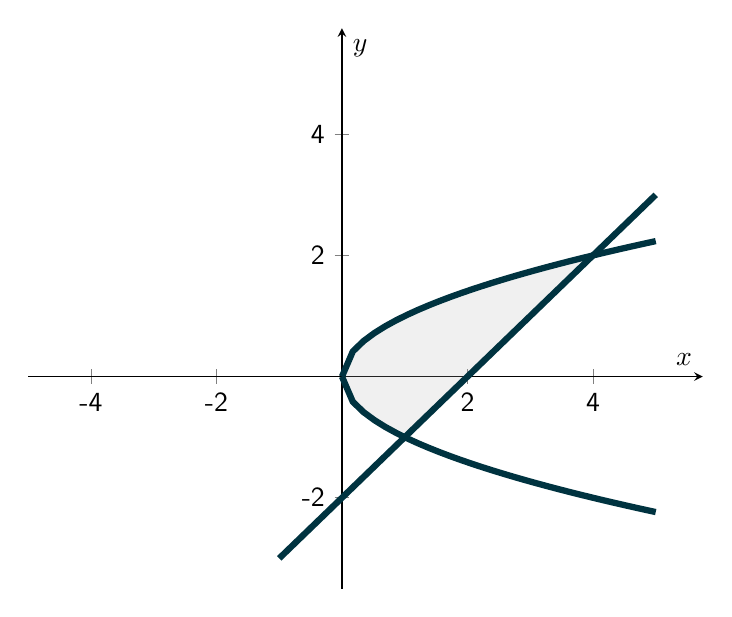
\begin{tikzpicture}[scale=1.25]
            \begin{axis}[
            axis lines = middle, very thick,
            xlabel = {$x$},
            ylabel = {$y$},
            xmin=-5, xmax=5.75,
            ymin=-3.5, ymax=5.75,
            xtick={-4,-2,0,2,4},
            xticklabels={-4,-2,0,2,4},
            ytick={-2,0,2,4},
            yticklabels={-2,0,2,4}        
            ]
            % Curves
            \addplot [name path = A,-,domain = 0:5, line width=0.8mm,DarkBlue,samples = 30] {sqrt(x)} ;
            \addplot [name path = B,-,domain = 0:5, line width=0.8mm,DarkBlue,samples = 30] {-sqrt(x)} ;
            \addplot [name path = C, line width=0.8mm, samples=4, smooth,domain=0:5, DarkBlue] coordinates {(-1,-3)(5,3)};
            % Fill area between paths
            \addplot [black!30, opacity=0.2] fill between [of = A and B, soft clip={domain=0:1}];
            \addplot [black!30, opacity=0.2] fill between [of = A and C, soft clip={domain=1:4}];
            \end{axis}
        \end{tikzpicture}    
    \end{center}   
        
    Thus
    \begin{align}
        \bar y &= \frac{M_x}M = \frac1M \int_{-1}^{2}\int_{y^2}^{y+2} 12y \, dx \, dy
    \end{align} 
    Thus
    \begin{align}
        a &= -1 \\
        b &= 2 \\
        c&= y^2 \\
        d&= y+2 \\
        f(x,y) &= \delta y = 12y
    \end{align}
    }
   \else

   \fi
    
\fi

\ifnum \Version=7
% SHORT SPHERICAL AND CYLINDRICAL EXERCISE
\part Point $P$ has rectangular (Cartesian) coordinates $(x,y,z) = (-6,0,8)$ in $\mathbb R^3$. In cylindrical coordinates, the point is $(r,\theta,z)$, and in spherical coordinates the point is $(\rho, \phi, \theta)$. Where $r=\framebox{\strut\hspace{1cm}}$, $\theta=\framebox{\strut\hspace{2cm}}$, $z=\framebox{\strut\hspace{1cm}}$, $\rho=\framebox{\strut\hspace{2cm}}$, and $\phi=\framebox{\strut\hspace{3cm}}$. 

    \ifnum \Solutions=1 {\color{DarkBlue} \textit{Solutions:} To convert to cylindrical we can use the equation $r^2 = x^2 + y^2$. 
    \begin{align}
        r^2 &= x^2 + y^2 = (-6)^2 + 0^2 = 36 \ \Rightarrow \ r = 6
    \end{align}
    To determine $\theta$ we can use $\tan\theta = y/x$. 
    \begin{align}
        \tan \theta &= \frac{y}{x} = \frac{0}{-6} = 0  \\
        \theta &= \arctan 0 
    \end{align} 
    The point in cylindrical is: 
    \begin{align}
        (r,\theta,z) &= (6,\pi,8) \\
        r &= 6 \\
        \theta &= \pi \\
        z &= 8
    \end{align}
    In spherical, we can start by obtaining $\rho$. 
    \begin{align}
        \rho^2 &= x^2+y^2+z^2\\
        \rho^2 &= (-6)^2 + 0^2 + 8^2 = 36+64 = 100 \\
        \rho &= 10
    \end{align}
    To obtain $\phi$ we can use the equation that relates $x$ to spherical. Using the expression for $x$, and the values that we already have for $x$, $\rho$ and $\theta$:
    \begin{align}
        x &= \rho \sin\phi \cos\theta \\
        -6 &= 10\sin\phi \cos(\pi) \\
        \sin\phi &= \frac{-6}{10 \cos(\pi)}  = \frac{6}{10}\\
        \phi &= \arcsin (6/10)
    \end{align}
    Our coordinates in spherical are
    \begin{align}
        \rho &= 10\\
        \phi &= \arcsin (6/10)\\
        \theta &= \pi
    \end{align}
    Note the following.
    \begin{itemize}
        \item We can, for this exercise, leave un-evaluated trig functions in the answer, because the question didn't specify that you should simplify your answer as much as possible. So it would be ok to leave your answer for $\theta$ as $\arctan 0$ or $\tan^{-1} 0$. 
        \item Our particular textbook uses the convention $(\rho, \phi, \theta)$, not $(\rho, \theta,\phi)$.
    \end{itemize}
    } 
    \else
      
    \fi
    
\fi





\ifnum \Version=8
% SHORT SPHERICAL AND CYLINDRICAL EXERCISE
\part Point $P$ has rectangular (Cartesian) coordinates $(x,y,z) = (4,4,7)$ in $\mathbb R^3$. In cylindrical coordinates, the point is $(r,\theta,z)$, and in spherical coordinates the point is $(\rho, \phi, \theta)$. Where $r=\framebox{\strut\hspace{1cm}}$, $\theta=\framebox{\strut\hspace{2cm}}$, $z=\framebox{\strut\hspace{1cm}}$, $\rho=\framebox{\strut\hspace{2cm}}$, and $\phi=\framebox{\strut\hspace{3cm}}$. 

    \ifnum \Solutions=1 {\color{DarkBlue} \textit{Solutions:} To convert to cylindrical we can use the equation $r^2 = x^2 + y^2$. 
    \begin{align}
        r^2 &= x^2 + y^2 = (4)^2 + 4^2 = 32 \ \Rightarrow \ r = \sqrt{32} = 4\sqrt2
    \end{align}
    It isn't necesssary to simplify to $4\sqrt2$. Then to determine $\theta$ we can use $\tan\theta = y/x$. 
    \begin{align}
        \tan \theta &= \frac{y}{x} = \frac{4}{4} = 1  \\
        \theta &= \arctan \pi/4
    \end{align} 
    The point in cylindrical is: 
    \begin{align}
        (r,\theta,z) &= (4\sqrt2,\pi/4,7) \\
        r &= 4\sqrt2 \\
        \theta &= \pi/4 \\
        z &= 7
    \end{align}
    In spherical, we can start by obtaining $\rho$. 
    \begin{align}
        \rho^2 &= x^2+y^2+z^2\\
        \rho^2 &= (4)^2 + 4^2 + 7^2 = 16+16+49 = 32+49 = 81 \\
        \rho &= 9
    \end{align}
    To obtain $\phi$ we can use the equation that relates $x$ to spherical. Using the expression for $x$, and the values that we already have for $x$, $\rho$ and $\theta$:
    \begin{align}
        x &= \rho \sin\phi \cos\theta \\
        4 &= 9\sin\phi \cos(\pi/4) \\
        \sin\phi &= \frac{4}{9 \cos(\pi/4)}  = \frac{4\sqrt2}{9}\\
        \phi &= \arcsin \left(\frac{4\sqrt2}{9}\right)
    \end{align}
    Note for $\phi$ we can also use:
    \begin{align}
        y &= \rho \sin\phi \sin\theta \\
        4 &= 9\sin\phi \sin(\pi/4) \\
        \sin\phi &= \frac{4}{9 \sin(\pi/4)}  = \frac{4\sqrt2}{9}\\
        \phi &= \arcsin \left(\frac{4\sqrt2}{9}\right)
    \end{align}    
    And we can also use:
    \begin{align}
        z &= \rho \cos\phi  \\
        7 &= 9\cos\phi  \\
        \sin\phi &= \frac{4}{9 \sin(\pi/4)}  = \frac{4\sqrt2}{9}\\
        \phi &= \arccos \left(\frac{7}{9}\right)
    \end{align}      
    Our coordinates in spherical are
    \begin{align}
        \rho &= 9\\
        \phi &= \arcsin \left(\frac{4\sqrt2}{9}\right), \ \textbf{or} \ \phi = \arccos(7/9)\\
        \theta &= \pi/4
    \end{align}
    Note the following.
    \begin{itemize}
        \item We can, for this exercise, leave un-evaluated trig functions in the answer, because the question didn't specify that you should simplify your answer as much as possible. So it would be ok to leave your answer for $\theta$ as $\arctan 1$ or $\tan^{-1} 1$. 
        \item Our particular textbook uses the convention $(\rho, \phi, \theta)$, not $(\rho, \theta,\phi)$.
    \end{itemize}
    } 
    \else
      
    \fi
    
\fi





% 15.6
% CENTROID Y-COORDINATE PARABOLA AND LINE
\ifnum \Version=9
    \part A thin plate with density $\delta=12$ is bounded in the $xy-$plane by $y=3-x^2$ and $y=1-x$. The plate has mass $M$. The $y-$coordinate of the centroid is $\bar y = M_x/M$, where $\displaystyle M_x = \int_A^B \int_C^D f(x,y) \, dy \, dx$,  and $A=\framebox{\strut\hspace{1cm}}$, $B=\framebox{\strut\hspace{1cm}}$, $C=\framebox{\strut\hspace{3cm}}$, $D=\framebox{\strut\hspace{3cm}}$, and $f(x,y) = \framebox{\strut\hspace{3cm}}$. 
    
    \ifnum \Solutions=1 
    {\color{DarkBlue}
    The region is bounded by 
    $$1-x \le y \le 3-x^2$$
    The given curves intersect when 
    \begin{align}
        1-x &= 3-x^2\\
        0 &= x^2-x-2 \\
        &= (x-2)(x+1)
    \end{align}
    The curves intersect at $x=-1,2$. Using $y=1-x$, the intersection points are $(-1,2)$ and $(2,-1)$. The region is shown below. 
    \begin{center}  
        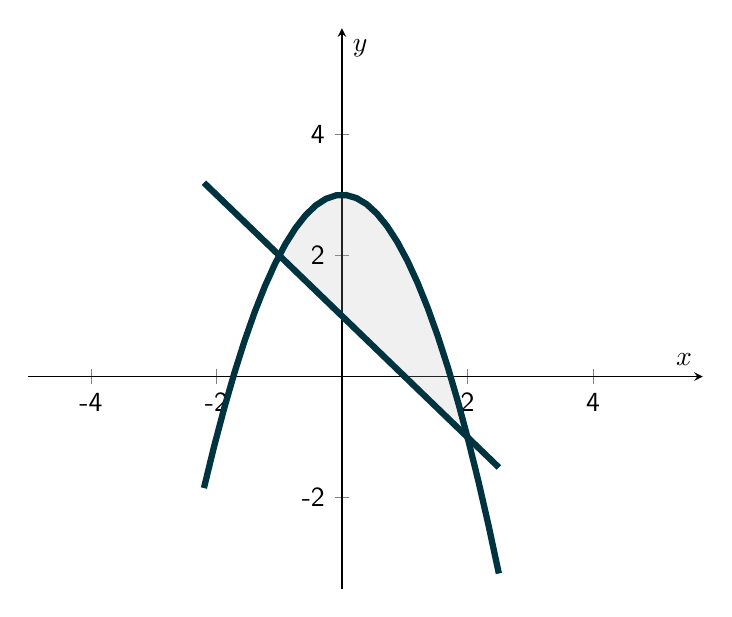
\begin{tikzpicture}[scale=1.25]
            \begin{axis}[
            axis lines = middle, very thick,
            xlabel = {$x$},
            ylabel = {$y$},
            xmin=-5, xmax=5.75,
            ymin=-3.5, ymax=5.75,
            xtick={-4,-2,0,2,4},
            xticklabels={-4,-2,0,2,4},
            ytick={-2,0,2,4},
            yticklabels={-2,0,2,4}        
            ]
            % Curves
            \addplot [name path = A,-,domain = -2.2:2.5, line width=0.8mm,DarkBlue,samples = 30] {3-x^2} ;
            \addplot [name path = C,-,domain = -2.2:2.5, line width=0.8mm,DarkBlue,samples = 4] {1-x} ;
            % Fill area between paths
            \addplot [black!30, opacity=0.2] fill between [of = A and C, soft clip={domain=-1:2}];
            \end{axis}
        \end{tikzpicture}    
    \end{center}   
        
    Thus
    \begin{align}
        \bar y &= \frac{M_x}M = \frac1M \int_{-1}^{2}\int_{1-x}^{3-x^2} 12y \, dy \, dx
    \end{align} 
    Thus
    \begin{align}
        A &= -1 \\
        B &= 2 \\
        C&= 1-x \\
        D&= 3-x^2 \\
        f(x,y) &= \delta y = 12y
    \end{align}
    }
   \else

   \fi
    
\fi
   
    % 13.3 and 13.4
% unit tangent vectors
% arc length
% curvature
% osculating circle
% unit normal

\ifnum \Version=1

\part The unit tangent vector for a curve $\mathbf r(t)$ is $\mathbf T(t) = \langle 0, \cos t, \sin t \rangle$. The unit normal vector is $\mathbf  N = \langle f(t), g(t), g(t) \rangle$, where $f(t) = \framebox{\strut\hspace{2cm}}$, $g(t) = \framebox{\strut\hspace{2cm}}$, $h(t) =\framebox{\strut\hspace{2cm}}$. 

\ifnum \Solutions=1 {\color{DarkBlue} \textit{Answer:} \textit{Solutions:} The normal vector is

\begin{align}
    \mathbf N &= \frac{d\mathbf T/dt}{|d\mathbf T/dt|} 
\end{align}
And
\begin{align}
    \mathbf T'(t) &= \langle 0,-\sin t, \cos t \rangle \\
    |\mathbf T'(t) | &= \sqrt{ 0 +(-\sin t)^2 + (\cos t)^2} =1\\
    \mathbf N &= \frac{d\mathbf T/dt}{|d\mathbf T/dt|} = \langle 0, - \sin(t),  \cos(t) \rangle
\end{align}
} 
\else
\fi        
\fi

\ifnum \Version=2

\part The velocity vector of an object moving on the curve $\mathbf r(t)$ is $\mathbf v(t) = \langle 4\cos (2t), 4\sin (2t) , 3 \rangle$ for $t>0$. The speed of the object for $t>0$ is $s(t) = |\mathbf v | = \framebox{\strut\hspace{1cm}}$. The unit tangent vector for $t>0$ is $\mathbf T = \langle f(t), g(t) , h(t) \rangle$, where $f(t) = \framebox{\strut\hspace{1.5cm}}$, $g(t) = \framebox{\strut\hspace{1.5cm}}$, $h = \framebox{\strut\hspace{1cm}}$. The curvature is $\kappa = \framebox{\strut\hspace{1cm}}$. 

\ifnum \Solutions=1 {\color{DarkBlue} \textit{Answer:} \textit{Solutions:} The speed is the magnitude of the given velocity vector and is
\begin{align}
    s &= |\mathbf v | =  \sqrt{(4\cos2t)^2 + (4\sin2t)^2 + 3^2 } = \sqrt{4^2 (\cos ^2 2 t + \sin^2 2t) + 3^2} = \sqrt{16 + 9} = 5
\end{align}
The unit tangent vector is 
\begin{align}
    \mathbf T &= \frac{\mathbf v}{|\mathbf v|} = \langle \frac{4}{5}\cos(2 t) , \frac 45 \sin (2t), \frac35 \rangle
\end{align}
For curvature we also need
\begin{align}
    \frac{d\mathbf T}{dt } &= \langle -\frac85 \sin 2t, \frac85 \cos 2t,0 \rangle \\
    \left | \frac{d\mathbf T}{dt } \right| &= \sqrt{ \left(-\frac85\sin 2t\right)^2 +   \left(\frac85 \cos 2 t\right)^2 } = \frac85
\end{align}
The curvature is
\begin{align}
    \kappa = \frac{1}{|\mathbf v |}\left| \frac{d\mathbf T}{dt}\right| = \frac{1}{5} \cdot \frac{8}{5} = \frac{8}{25}
\end{align}
} 
\else
\fi        
\fi


\ifnum \Version=3

\part A plane curve $\mathbf r(t)$ has curvature $\kappa = \frac{1}{8}$ at $\mathbf r(t_0) = \langle 15, 2 \rangle$, and the unit normal vector at $t=t_0$ is $\mathbf  N = \mathbf j = \langle 0, 1 \rangle$. The equation of the osculating circle at $t=t_0$ is \framebox{\strut\hspace{3.5cm}}.

\ifnum \Solutions=1 {\color{DarkBlue} \textit{Answer:} \textit{Solutions:} Recall that The circle of curvature, or osculating circle, at a point $P$ on a plane curve where $\kappa \ne 0$ is the circle in the plane of the curve that

\begin{enumerate}
    \item is tangent to the curve at P (has the same tangent line the curve has)
    \item has the same curvature the curve has at P
    \item lies toward the concave or inner side of the curve
\end{enumerate}
The \textbf{radius of curvature} of the curve at P is the radius of the circle of curvature, which is $\frac{1}{\kappa}$. So to obtain the radius, we calculate $\kappa$ and take the reciprocal. The \textbf{center} of the osculating circle of the curve at P lies on the inner side of the curve, and the unit normal points in the direction of the inner side of the planar curve. 

So for this problem we have a circle with radius $1/\kappa = 8$, and whose centre is 8 units away from the point $(15,2)$ in the direction of $\mathbf N$. The circle has equation
$$(x-15)^2 + (y-10)^2 = 8^2$$
} 
\else
  
\fi        
\fi




\ifnum \Version=4

\part The velocity vector for an object moving on the curve $\mathbf r(t)$ is $\mathbf v(t) = \langle t\cos t, t\sin t \rangle$. The speed of the object for $t>0$ is $s(t) = \framebox{\strut\hspace{1cm}}$. The unit tangent vector for $t>0$ is $\mathbf T = \langle f(t), g(t) \rangle$, where $f(t) = \framebox{\strut\hspace{2cm}}$, $g(t) = \framebox{\strut\hspace{2cm}}$. 

\ifnum \Solutions=1 {\color{DarkBlue} \textit{Answer:} \textit{Solutions:} The speed is the magnitude of the velocity vector and is
\begin{align}
    s &= |\mathbf v | = \sqrt{(t\cos t)^2 + (t\sin t)^2 } = \sqrt{t^2 (\cos ^2 t + \sin^2 t)} = |t|
\end{align}
But we are told that $t>0$ so we can use $|t| = t$. The unit tangent vector is 
\begin{align}
    \mathbf T &= \frac{\mathbf v}{|\mathbf v|} = \langle \cos t, \sin t \rangle
\end{align}
} 
\else
\fi        
\fi

\ifnum \Version=5

\part A plane curve $\mathbf r(t)$ has curvature $\kappa = \frac{1}{4}$ at the point $\mathbf r(t_0) = 3\mathbf i + 5\mathbf j$, and the unit normal vector at $t_0$ is $\mathbf  N = \mathbf i = \langle1,0\rangle$. The equation of the osculating circle at $t=t_0$ is \framebox{\strut\hspace{3.5cm}}.

\ifnum \Solutions=1 {\color{DarkBlue} \textit{Answer:} \textit{Solutions:} Recall that The circle of curvature, or osculating circle, at a point $P$ on a plane curve where $\kappa \ne 0$ is the circle in the plane of the curve that

\begin{enumerate}
    \item is tangent to the curve at P (has the same tangent line the curve has)
    \item has the same curvature the curve has at P
    \item lies toward the concave or inner side of the curve
\end{enumerate}
The \textbf{radius of curvature} of the curve at P is the radius of the circle of curvature, which is $\frac{1}{\kappa}$. So to obtain the radius, we calculate $\kappa$ and take the reciprocal. The \textbf{center} of the osculating circle of the curve at P lies on the inner side of the curve, and the unit normal points in the direction of the inner side of the planar curve. 

So for this problem we have a circle with radius $1/\kappa = 4$, and whose centre is 4 units away from the point $(3,5)$ in the direction of $\mathbf N$. The circle has equation
$$(x-7)^2 + (y-5)^2 = 4^2$$
} 
\else
  
\fi        
\fi


\ifnum \Version=6

\part The velocity vector for an object moving on the curve $\mathbf r(t)$ is $\mathbf v(t) = \langle 4t\cos t, 4t\sin t \rangle$ for $t>0$. The speed of the object for $t>0$ is $s(t)  = |\mathbf v | = \framebox{\strut\hspace{1cm}}$. The unit tangent vector for $t>0$ is $\mathbf T = \langle f(t), g(t) \rangle$, where $f(t) = \framebox{\strut\hspace{1.5cm}}$, $g(t) = \framebox{\strut\hspace{1.5cm}}$. The curvature is $\kappa = \framebox{\strut\hspace{1cm}}$. 

\ifnum \Solutions=1 {\color{DarkBlue} \textit{Answer:} \textit{Solutions:} The speed is the magnitude of the given velocity vector and is
\begin{align}
    s &= |\mathbf v | =  \sqrt{(4t\cos t)^2 + (4t\sin t)^2 } = \sqrt{4^2t^2 (\cos ^2 t + \sin^2 t)} = 4|t|
\end{align}
But we are told that $t>0$ so we can assume $|t| = t$. The unit tangent vector is 
\begin{align}
    \mathbf T &= \frac{\mathbf v}{|\mathbf v|} = \langle \cos t, \sin t \rangle
\end{align}
We need
\begin{align}
    \frac{d\mathbf T}{dt } &= \langle -\sin t, \cos t \rangle \\
    \left | \frac{d\mathbf T}{dt } \right| &= \sqrt{ (-\sin t)^2 +   \cos^2 t } = 1
\end{align}
The curvature is
\begin{align}
    \kappa = \frac{1}{|\mathbf v |}\left| \frac{d\mathbf T}{dt}\right| = \frac{1}{4t} 
\end{align}
} 
\else
\fi        
\fi



\ifnum \Version=7

\part The velocity vector of an object moving on the curve $\mathbf r(t)$ is $\mathbf v(t) = \langle 3\cos (2t), 3\sin (2t) \rangle$ for $t>0$. The speed of the object for $t>0$ is $s(t) = |\mathbf v | = \framebox{\strut\hspace{1.5cm}}$. The unit tangent vector for $t>0$ is $\mathbf T = \langle f(t), g(t)  \rangle$, where $f(t) = \framebox{\strut\hspace{2cm}}$, and $g(t) = \framebox{\strut\hspace{2cm}}$.  The curvature for $t>0$ is \framebox{\strut\hspace{1.5cm}}. 

\ifnum \Solutions=1 {\color{DarkBlue} \textit{Answer:} \textit{Solutions:} The speed is the magnitude of the given velocity vector and is
\begin{align}
    s &= |\mathbf v | =  \sqrt{(3\cos t)^2 + (3\sin t)^2  } = \sqrt{3^2 (\cos ^2 t + \sin^2 t) + 3^2} = \sqrt{ 9} = 3
\end{align}
The unit tangent vector is 
\begin{align}
    \mathbf T &= \frac{\mathbf v}{|\mathbf v|} 
    = \langle \frac{3}{3}\cos(2 t) , \frac 33 \sin (2t) \rangle 
    = \langle \cos(2 t) ,  \sin (2t) \rangle
\end{align}
For curvature we also need
\begin{align}
    \frac{d\mathbf T}{dt } &= \langle -2 \sin 2t, 2 \cos 2t\rangle \\
    \left | \frac{d\mathbf T}{dt } \right| &= \sqrt{ \left(-2\sin 2t\right)^2 +   \left(2 \cos 2 t\right)^2 } = 2
\end{align}
The curvature is
\begin{align}
    \kappa = \frac{1}{|\mathbf v |}\left| \frac{d\mathbf T}{dt}\right| = \frac{1}{3} \cdot 2 = \frac{2}{3}
\end{align}
} 
\else
\fi        
\fi


\ifnum \Version=8

\part A plane curve $\mathbf r(t)$ has curvature $\kappa = \frac{1}{4}$ at $\mathbf r(t_0) = \langle 5, 3 \rangle$, and the unit normal vector at $t=t_0$ is $\mathbf  N = \mathbf j = \langle 0, 1 \rangle$. The equation of the osculating circle at $t=t_0$ is \framebox{\strut\hspace{3.5cm}}.

\ifnum \Solutions=1 {\color{DarkBlue} \textit{Answer:} \textit{Solutions:} Recall that The circle of curvature, or osculating circle, at a point $P$ on a plane curve where $\kappa \ne 0$ is the circle in the plane of the curve that

\begin{enumerate}
    \item is tangent to the curve at P (has the same tangent line the curve has)
    \item has the same curvature the curve has at P
    \item lies toward the concave or inner side of the curve
\end{enumerate}
The \textbf{radius of curvature} of the curve at P is the radius of the circle of curvature, which is $\frac{1}{\kappa}$. So to obtain the radius, we calculate $\kappa$ and take the reciprocal. The \textbf{center} of the osculating circle of the curve at P lies on the inner side of the curve, and the unit normal points in the direction of the inner side of the planar curve. 

So for this problem we have a circle with radius $1/\kappa = 4$, and whose centre is 4 units away from the point $(5,3)$ in the direction of $\mathbf N$. The circle has equation
$$(x-5)^2 + (y-7)^2 = 4^2$$
} 
\else
  
\fi        
\fi






\ifnum \Version=9

\part The velocity vector of an object moving on the curve $\mathbf r(t)$ is $\mathbf v(t) = \langle t, 3 \rangle$ for $t>0$. The speed of the object at $t=2$ is $s(2) = |\mathbf v(2) | = \framebox{\strut\hspace{1.75cm}}$. The unit tangent vector at $t=2$ is $\mathbf T(2) = \langle c_1 ,c_2  \rangle$, where $c_1 = \framebox{\strut\hspace{1.75cm}}$, $c_2 = \framebox{\strut\hspace{1.75cm}}$. The curvature is $\framebox{\strut\hspace{1.75cm}}$. 

\ifnum \Solutions=1 {\color{DarkBlue} \textit{Answer:} \textit{Solutions:} The speed is the magnitude of the given velocity vector and is
\begin{align}
    s &= |\mathbf v | =  \sqrt{( t)^2 + (3)^2  } = \sqrt{t^2+9}\\
    s(2) &= \sqrt{2^2+9} = \sqrt{13}
\end{align}
We also need the unit tangent vector at $t=2$. 
\begin{align}
    \mathbf T (t) &= \frac{\mathbf v}{|\mathbf v|} = \frac{t\mathbf i + 3\mathbf j}{\sqrt{t^2+9}} \\
    \mathbf T (2) &= \frac{2\mathbf i + 3\mathbf j}{\sqrt{2^2+9}}  
    = \langle \frac{2}{\sqrt{13}} , \frac {3}{\sqrt{13}}  \rangle \\
    c_1 &= \frac{2}{\sqrt{13}}\\
    c_2 &= \frac{3}{\sqrt{13}}
\end{align}
The curvature is zero because the motion is along a straight line. 
\begin{align}
    \kappa = 0
\end{align}
} 
\else
\fi        
\fi

\ifnum \Version=10

\part A plane curve $\mathbf r(t)$ has curvature $\kappa = \frac{1}{10}$ at $\mathbf r(t_0) = \langle 5, 0 \rangle$, and the unit normal vector at $t=t_0$ is $\mathbf  N = \mathbf j = \langle 0, 1 \rangle$. The equation of the osculating circle at $t=t_0$ is \framebox{\strut\hspace{3.5cm}}.

\ifnum \Solutions=1 {\color{DarkBlue} \textit{Answer:} \textit{Solutions:} Recall that The circle of curvature, or osculating circle, at a point $P$ on a plane curve where $\kappa \ne 0$ is the circle in the plane of the curve that

\begin{enumerate}
    \item is tangent to the curve at P (has the same tangent line the curve has)
    \item has the same curvature the curve has at P
    \item lies toward the concave or inner side of the curve
\end{enumerate}
The \textbf{radius of curvature} of the curve at P is the radius of the circle of curvature, which is $\frac{1}{\kappa}$. So to obtain the radius, we calculate $\kappa$ and take the reciprocal. The \textbf{center} of the osculating circle of the curve at P lies on the inner side of the curve, and the unit normal points in the direction of the inner side of the planar curve. 

So for this problem we have a circle with radius $1/\kappa = 10$, and whose centre is 10 units away from the point $(5,0)$ in the direction of $\mathbf N$. The circle has equation
$$(x-5)^2 + (y-10)^2 = 10^2$$
} 
\else
  
\fi        
\fi
   
\end{parts}

\newpage \question[0.25] \ID
% CHANGE OF VARIABLE (15.8)
% OR APPLICATION (15.6)
% OR TRIPLE CARTESIAN (15.5) 

\ifnum \Version=1
% CENTROID
% BASED ON THOMAS EXERCISES, 15.6 #1
% SUFFICIENT FOR A PRACTICE EXAM
\question[6] A thin plate of density $\delta(x,y) = 12x$ is bounded by the lines $x = 0, y = x$, and the parabola $y = x^2-6$ in the first quadrant. 
\begin{parts} 
    \part Determine the mass of the plate, $M$. Please show your work. 
    \ifnum \Solutions=1 
    {\color{DarkBlue} \textit{Solutions:}
    Curves intersect when $$x = x^2-6 \quad \Rightarrow \quad 0 = x^2 - x - 6 = (x-3)(x+2)$$
    Or $x=3, -2$. We can ignore $x=-2$ because the region is the first quadrant. Curves intersect at the point $(3,3)$, and 
    \begin{align}
        0 \le y \le 3, \quad y \le x \le \sqrt{y+6}
    \end{align}
    The mass is
    \begin{align}
        M &= \int_0^3 \int_y^{\sqrt{y+6}} \delta \, dx \, dy \\
        &= \int_0^3 \int_y^{\sqrt{y+6}} 12x \, dx \, dy \\
        &= \int_0^3  \left. 6x^2 \right|_{x=y}^{x=\sqrt{y+6}} \, dy \\
        &= \int_0^3 6(y + 6 - y^2) \, dy \\
        &= \int_0^3 6y + 36 - 6y^2 \, dy \\
        &= \left. (3y^2 + 36y - 2y^3 ) \right|_0^3 \, dy \\
        &= 27 + 108 - 54 \\
        &= 81
    \end{align}
    }
    \else 
    \vspace{16cm}
    \fi
    \part Use your results from the previous part to set up an integral that can be used to determine the $x-$coordinate of the center of mass of the plate. You do not need to evaluate your integral. 
    \ifnum \Solutions=1 {\color{DarkBlue} \textit{Solutions:} the $x-$coordinate of the center of mass, $\bar x$, is
    \begin{align}
    \bar x &= \frac{M_y}{M} = \frac{1}{81} \int_0^3 \int_y^{\sqrt{y+6}} 12x^2 \, dx \, dy 
    \end{align}
    } 
    \else
      
    \fi
    \end{parts} 
\fi
    





\ifnum \Version=2
% LONGISH CHANGE OF VARIABLE
% VERBATUM FROM SPRING 2022 QUIZ
% hand written solution only
% SUFFICIENT FOR A PRACTICE EXAM
\question[6] Consider the double integral

$$I=\iint_R \frac{x+2y}{2y-x} dA$$

where $R$ is the parallelogram with vertices $(-3,1), (-1,0), (-1,2), (1,1)$. Our goal is to determine the area of the parallelogram using the transform below. 
$$u=x+2y, \qquad v = -x +2y$$ 
Please show your work for the following. 
\begin{parts} 
    \part Use the given transform to calculate the Jacobian of the transform, $J = \partial x(u,v)/\partial y(u,v)$. 
    \ifnum \Solutions=1 
    \else 
    \vspace{8 cm}
    \fi
    \part Use your results from Part (a) and the given transform to transform the double integral. You do not need to evaluate your integral. 
\end{parts} 

\ifnum \Solutions=1 {\color{DarkBlue} \textit{Solutions:} the integral after the transform is $$\displaystyle \frac14 \int_1^5\int_{-1}^3 \frac uv \, du \, dv$$
A screen capture of a hand-written solution from a previous offer of MATH 2551 is below. 
    \begin{figure}[h]
    \centering
    \includegraphics[width=16cm]{202302/Exam3/Images/ImgE3.OR.06.png}
    \end{figure}  
    
    } 
   \else
      
   \fi
    
\fi

\ifnum \Version=3
% CENTROID
% BASED ON THOMAS EXERCISES, 15.6 #1
% SUFFICIENT FOR A PRACTICE EXAM
\question[6] A thin plate with density $\delta(x,y) = 24y$ is bounded by the lines $x = 0, x=2y$, and the parabola $x=y^2$ in the first quadrant. 
\begin{parts} 
    \part Determine the mass of the plate, $M$. Please show your work. 
    
    \ifnum \Solutions=1 
    {\color{DarkBlue} \textit{Solutions:}
    Curves intersect when $$2y = y^2 \quad \Rightarrow \quad 0 = y^2-2y = y(y-2)$$
    Or $y=0,2$. Curves intersect at the points $(0,0)$, $(4,2)$. 
    The mass is
    \begin{align}
        M = \int_0^4 \int_{x/2}^{\sqrt{x}} \delta \, dy \, dx 
        &= \int_0^4 \int_{x/2}^{\sqrt{x}} 24y \, dy \, dx \\
        &= \int_0^4  \left. 12y^2 \right|_{y=x/2}^{y=\sqrt{x}} \, dx \\
        &= 12 \int_0^4 (x-\frac{x^2}{4}) \, dx \\
        &= 12 \left. (\frac{x^2}{2} - \frac{x^3}{12} ) \right|_0^4 \, dy \\
        &= 12 (\frac{16}{2} - \frac{64}{12}) \\
        &= 96 - 64\\
        &= 32
    \end{align}
    \textbf{An Alternate Solution}\\
    Another way to approach this problem is to use the integration order $dx\,dy$. In this case the double integral becomes
    \begin{align}
        M = \int_0^2 \int_{y^2}^{2y} \delta \, dx \, dy
        &= \int_0^2 \int_{y^2}^{2y} 24y \, dx \, dy \\
        &= 24\int_0^2  \left. yx \right|_{x=y^2}^{x=2y} \, dy \\
        &= 24 \int_0^2 (2y^2 - y^3) \, dy \\
        &= 24 \left. (\frac{2y^3}{3} - \frac{y^4}{4} ) \right|_0^2 \, dy \\
        &= 24 (\frac{16}{3} - \frac{16}{4}) \\
        &= \frac{24\cdot16}{3} - 24\cdot 4 \\
        &= 8\cdot16 - 96 \\
        &= 128 - 96 \\
        &= 32
    \end{align}    
    }
    \else 
    \vspace{14cm}
    \fi
    \part Use your results from the previous part to set up an integral that can be used to determine the $x-$coordinate of the center of mass of the plate. You do not need to evaluate your integral. 
    \ifnum \Solutions=1 {\color{DarkBlue} \textit{Solutions:} the $x-$coordinate of the center of mass, $\bar x$, is
    \begin{align}
    \bar x &= \frac{M_y}{M} = \frac{1}{32} \int_0^4 \int_{x/2}^{\sqrt{x}} 24xy \, dy \, dx
    \end{align}
    \textbf{An Alternate Solution}\\    
    It is also ok to use the integration order $dx\,dy$. In this case the double integral becomes
    \begin{align}
    \bar x &= \frac{M_y}{M} = \frac{1}{32} \int_0^2 \int_{y^2}^{2y} 24xy \, dx \, dy 
    \end{align}
    } 
    \else
      
    \fi
    \end{parts} 
\fi

\ifnum \Version=4
% VERSION B
% LONG CHANGE OF VARIABLE
% BASED ON AN EXAMPLE FROM THOMAS
% SECTION 15.8 FROM THOMAS
\question[6] Consider the double integral

$$I= 9 \iint_R (y-2x)^2 \sqrt{x+y} \, dA$$

where $R$ is the region in the first quadrant bounded by the lines $x=0$, $y=0$, and $y=1-x$. Our goal is to determine the area of $R$ using the transform below. 
$$u=x+y, \qquad v = y-2x$$ 
Please show your work for the following. 
\begin{parts} 
    \part Use the given transform to calculate the Jacobian of the transform, $J = \partial x(u,v)/\partial y(u,v)$. 
    \ifnum \Solutions=1 {\color{DarkBlue} \textit{Solutions:} Solving for $x$ and $y$ using an augmented matrix,
    \begin{align}
        \begin{pmatrix} 1 & 1 & u \\-2 & 1 & v\end{pmatrix} 
        \sim \begin{pmatrix} 1 & 1 & u \\0 & 3 & 2u+v\end{pmatrix} 
        \sim \begin{pmatrix} 1 & 0 & u/3 - v/3 \\0 & 1 & 2u/3+v/3 \end{pmatrix} 
    \end{align}
    Thus
    \begin{align}
        x &= \frac13(u-v), \ y = \frac13(2u+v) \\
        J(u,v) & = \begin{vmatrix} \DXDU & \DXDV \\[8pt] \DYDU & \DYDV \end{vmatrix} = \begin{vmatrix} 1/3 & -1/3 \\ 2/3 & 1/3 \end{vmatrix} = 1/9 + 2/9 = 1/3
    \end{align}
    }
    \else 
    \vspace{8 cm}
    \fi
    \part Use the given transform and your results from Part (a) to convert the double integral into a double integral over a region in the $uv-$plane. You do not need to evaluate your integral. 
    \ifnum \Solutions=1 {\color{DarkBlue} \textit{Solutions:} Converting each of the boundaries in the $xy-$plane into the $uv-$plane we obtain
        \begin{align}
            x+y &= 1 \quad \Rightarrow \quad \frac13(u-v) + \frac13(2u+v) = 1 &&\Rightarrow \quad u = 1\\
            x&=0 \quad \Rightarrow \quad \frac13(u-v) = 0 &&\Rightarrow \quad v = u\\
            y&= 0 \quad \Rightarrow \quad \frac13(2u+v) = 0 &&\Rightarrow \quad v = -2u
        \end{align}
        The region is described by either of the following relations:
        \begin{align}
            S_1: & \quad 0 \le u \le 1, \quad -2u \le v \le u \\
            S_2: & \quad -2 \le v \le 0, \quad -v/2 \le u \le 1, \ \text{and } 0 \le v \le 1, \quad v \le u \le 1
        \end{align}
        The first set of inequalities requires only a single double integral, but it is ok to set up two double integrals. If using $S_1$, we use $dv\,du$ and obtain
        \begin{align}
            I= 9 \iint_R (y-2x)^2 \sqrt{x+y} \, dA = 9 \int_0^1 \int_{-2u}^u v^2u^{1/2} \frac13 \,dv\,du
        \end{align}
        If using $S_2$, we use $du\,dv$ and obtain
        \begin{align}
            I= 9 \iint_R (y-2x)^2 \sqrt{x+y} \, dA 
            = 9 \int_{-2}^0 \int_{-v/2}^1 v^2u^{1/2} \frac13 \,du\,dv
            + 9 \int_{0}^1 \int_{v}^1 v^2u^{1/2} \frac13 \,du\,dv
        \end{align}        
        } 
       \else
          
       \fi
    \end{parts} 

    \fi



\ifnum \Version=5
    % USE FOR VERSION B
    % LONG CYLINDRICAL WITH APPLICATION TO MASS WITH VARYING DENSITY
    % FROM 15.8
    \question[6] An object $D$ lying in the first octant is bounded below by the $xy-$plane, above by the plane $z=3+4y$, and by the cylinder $x^2+y^2 = 4$. The density of the object at any point in $D$ is equal to the distance from the point to the $z$-axis.  Please show your work for the following.
    
    \begin{parts} 
    \part Use cylindrical coordinates to calculate the total of mass of the object, $M$. Please show your work. 
    
    \ifnum \Solutions=1 {\color{DarkBlue} The object is only in the first octant so $$0 \le \theta \le \pi/2$$ Using $\delta = \sqrt{x^2+y^2} = r$, the $z-$coordinate of the center of mass is computed using 
    \begin{align}
        M &= \iiint_D  \delta \, dV \\
        &= \int_0^{\pi/2} \int_0^2 \int_0^{3+4r\sin\theta}  \delta(r,\theta) \, r\, dz\,dr\,d\theta\\
        &= \int_0^{\pi/2} \int_0^2 \int_0^{3+4r\sin\theta}   r^2 \, dz\,dr\,d\theta\\
        &= \int_0^{\pi/2} \int_0^2    r^2 \, (3+4r\sin\theta) \,dr\,d\theta \\
        &= \int_0^{\pi/2} \int_0^2     \, (3r^2+4r^3\sin\theta) \,dr\,d\theta \\
        &= \int_0^{\pi/2}  \left. \, (r^3+r^4\sin\theta) \right|_{r=0}^{r=2} d\theta \\
        &= \int_0^{\pi/2}  (8 + 16\sin\theta) d\theta \\
        &=  \left. (8\theta - 16\cos\theta) \right|_0^{\pi/2} \\
        &=  (4\pi - 0) - (0 - 16) \\
        &= 4\pi + 16
    \end{align}
    
    } 
    \else
        \vspace{14cm}
    \fi
    
    \part Use your results from the previous part to set up a triple integral in cylindrical coordinates that can be used to determine the $z-$coordinate of the center of mass of the object. You do not need to evaluate your integral. 

    \ifnum \Solutions=1 {\color{DarkBlue} \textit{Solutions:} the $z-$coordinate of the center of mass, $\bar x$, is
    \begin{align}
    \bar z &= \frac{M_{xy}}{M} = \frac{1}{16\pi+16} \int_0^{\pi/2} \int_0^2 \int_0^{3+4r\sin\theta}  z \, \delta(r,\theta) \, r\, dz\,dr\,d\theta
    \end{align}
    } 
    \else
      
    \fi
    \end{parts} 
\fi


% TRANSFORM: SOLVE FOR X & Y, BOUNDARIES, EVALUATE, TRIANGLES
% VERSION A
\ifnum \Version=6
    \question[6] Consider the transform $u=x+y$ and $v=4x+5y$, and the integral $\displaystyle I = \iint_{R}  \,dxdy$. Region $R$ is the triangle in the $xy$-plane bounded by $x+y=0$, $4x+5y=0$, $6x+7y=4$. The transform maps $R$ to region $G$ in the $uv-$plane.  Please show your work for the following.

    \begin{enumerate}
        \item[a)] Solve the system, $u=x+y$ and $v=4x+5y$, for $x$ and $y$ in terms of $u$ and $v$.
            \ifnum \Solutions=1 {\color{DarkBlue} \\[12pt] 
            \textbf{Solutions:}
            We can use the expressions for $u$ and $v$ as an augmented matrix and row reduce. 
            \begin{align}
                \begin{pmatrix} 1 & 1 & u \\ 4 & 5 & v\end{pmatrix} 
                \sim \begin{pmatrix} 1 & 1 & u \\0 & 1 & v - 4u \end{pmatrix} 
                \sim \begin{pmatrix} 1 & 0 & 5u - v \\ 0 & 1 & v - 4u \end{pmatrix} 
            \end{align}
            Thus $x = 5u - v$, and $y = v - 4u$. 
            } 
            \else 
            \vspace{5cm}
            \fi
        \item[b)] Transform the boundaries of $R$ to the $uv-$plane. In other words, determine the boundaries of $G$ in terms of $u$ and $v$. 
            \ifnum \Solutions=1 {\color{DarkBlue} \\[12pt] 
            \textbf{Solutions:} the three lines are transformed below. 
            \begin{itemize}
                \item The line $x+y=0$ becomes $u=0$. 
                \item The line $4x+5y=0$ becomes $v=0$. 
                \item The line $6x+7y=4$ is: 
                \begin{align}
                    6x+7y &=4 \\
                    6\cdot(5u-v) + 7\cdot(v-4u) &= 4\\
                    30u -28u -6v+7v &=4 \\
                    v &= 4 -2u
                \end{align}
            \end{itemize}
            } 
        \else 
        \vspace{5cm}
        \fi        
            
        \item[c)] Use the given transformation and your results from parts (a) and (b) to set up a double integral that in the $uv-$plane that is equal to $I$. Do not evaluate the integral. You also do not need to calculate the Jacobian and may use that the Jacobian of the transform is $J(u,v) = 1$.
            \ifnum \Solutions=1 {\color{DarkBlue} \\[12pt] 
            \textbf{Solutions:}
            \begin{align}
                \iint_{R} \,dx\,dy
                &= \iint_{G}  \left| J(u,v) \right| \,dv\,du 
                = \int_0^2\int_{0}^{4-2u}  \left| 1 \right| \,dv\,du 
                = \int_0^2\int_{0}^{4-2u} \,dv\,du
            \end{align}
            Note the following.
            \begin{itemize}
                \item We did not need to compute the Jacobian but it is computed as follows. 
                $$J 
                = \begin{vmatrix} x_u & x_v \\ y_u & y_v \end{vmatrix} 
                = \begin{vmatrix} 5 & -1 \\ -4 & 1\end{vmatrix} 
                = 5 - 4
                = 1$$
                \item             We did not need to evaluate the integral but if we did:
            \begin{align}
                I = \int_0^2\int_{0}^{4-2u}  \left| 1 \right| \,dv\,du
                = 1 \int_0^2 (4-2u) \,du
                =  \left. 4u - u^2 \right|_0^2 
                = 4
            \end{align}
            \item It is also ok to use the other integration order: $I = \int_0^4\int_0^{2-v/2} \, du \, dv$.
            \end{itemize}
            } 
            \else 
            \fi        
    \end{enumerate}
 
\fi 



% TRANSFORM: SOLVE FOR X & Y, BOUNDARIES, EVALUATE, PARALLELOGRAM
% VERSION A
\ifnum \Version=7
    \question[6] Consider the integral $\displaystyle I = 2\iint_{R} x-4y \,dx\,dy$, where $R$ is the parallelogram in the $xy$-plane bounded by $x-4y=2$, $x-4y=1$, $3y-x=3$, $3y-x=6$. Suppose the transform $u=x-4y$ and $v=3y-x$, maps region $R$ to region $G$ in the $uv-$plane.  Please show your work for the following.

    \begin{enumerate}
        \item[a)] Solve the system, $u=x-4y$ and $v=3y-x$, for $x$ and $y$ in terms of $u$ and $v$.
            \ifnum \Solutions=1 {\color{DarkBlue} \\[12pt] 
            \textbf{Solutions:}
            We can use the expressions for $u$ and $v$ as an augmented matrix and row reduce. 
            \begin{align}
                \begin{pmatrix} 1 & -4 & u \\ -1 & 3 & v\end{pmatrix} 
                \sim \begin{pmatrix} 1 & -4 & u \\0 & -1 & v + u\end{pmatrix} 
                \sim \begin{pmatrix} 1 & 0 & -3u-4v\\0 & 1 & -u-v\end{pmatrix} 
            \end{align}
            Thus
            \begin{align}
                x &=  -3u-4v\\
                y &= -u-v
            \end{align}

            } 
            \else 
            \vspace{5cm}
            \fi
        \item[b)] Transform the boundaries of $R$ to the $uv-$plane. In other words, determine the boundaries of $G$ in terms of $u$ and $v$. 
            \ifnum \Solutions=1 {\color{DarkBlue} \\[12pt] 
            \textbf{Solutions:} the four lines are transformed below. 
            \begin{itemize}
                \item The line $x-4y=2$ becomes $u=2$. 
                \item The line $x-4y=1$ becomes $u=1$. 
                \item The line $3y-x=3$ becomes $v=3$. 
                \item The line $3y-x=6$ becomes $v=6$. 
            \end{itemize}
            } 
        \else 
        \vspace{5cm}
        \fi        
            
        \item[c)] Use the given transformation and your results from parts (a) and (b) to set up a double integral that in the $uv-$plane that is equal to $I$. Do not evaluate the integral. You also do not need to calculate the Jacobian and may use that the Jacobian of the transform is  $J(u,v) = -1$. 
            \ifnum \Solutions=1 {\color{DarkBlue} \\[12pt] 
            \textbf{Solutions:}
            \begin{align}
                \iint_{R} 2x-8y \,dx\,dy
                = \iint_{G} 2u \left| J(u,v) \right| \,du\,dv
                = \int_3^6\int_{1}^2 2u \left| -1 \right| \,du\,dv
                = \int_3^6\int_{1}^2 2u \,du\,dv
            \end{align}
            Note the following.
            \begin{itemize}
                \item We did not need to evaluate the integral, but if we did: 
                \begin{align}
                \iint_{R} 2x-8y \,dx\,dy
                &= \iint_{G} 2u \left| J(u,v) \right| \,du\,dv\\
                &= \int_3^6\int_{1}^2 2u \left| -1 \right| \,du\,dv\\
                &= \int_3^6\left. u^2 \right|_{1}^2 \,dv\\
                &= \int_3^6 3 \,dv\\
                &= 3 \cdot(6 -3) \\
                &= 9
            \end{align}
            \end{itemize}
            } 
            \else 
            \fi        
    \end{enumerate}
 
\fi 




% TRANSFORM: SOLVE FOR X & Y, BOUNDARIES, EVALUATE
% VERSION B
\ifnum \Version=8
    \question[6] Consider the transform $u=x-y$ and $v=4y-2x$, and the integral $\displaystyle I = \iint_{R} \,dxdy$, where $R$ denotes the triangle in the $xy$-plane bounded by $x-y=2$, $4y-2x=0$, $3y=2x$. The transform maps region $R$ to region $G$ in the $uv-$plane.  Please show your work for the following.

    \begin{enumerate}
        \item[a)] Solve the system, $u=x-y$ and $v=4y-2x$, for $x$ and $y$ in terms of $u$ and $v$.
            \ifnum \Solutions=1 {\color{DarkBlue} \\[12pt] 
            \textbf{Solutions:}
            We can use the expressions for $u$ and $v$ as an augmented matrix and row reduce. 
            \begin{align}
                \begin{pmatrix} 1 & -1 & u \\ -2 & 4 & v\end{pmatrix} 
                \sim \begin{pmatrix} 1 & -1 & u \\0 & 2 & v + 2u\end{pmatrix} 
                \sim \begin{pmatrix} 1 & -1 & u\\0 & 1 & u+v/2\end{pmatrix} 
                \sim \begin{pmatrix} 1 & 0 & 2u+v/2\\0 & 1 & u+v/2\end{pmatrix} 
            \end{align}
            Thus $x = 2u+v/2$, and $y = u + \frac{v}{2}$. 
            } 
            \else 
            \vspace{5cm}
            \fi
        \item[b)] Transform the boundaries of $R$ to the $uv-$plane. In other words, determine the boundaries of $G$ in terms of $u$ and $v$. 
            \ifnum \Solutions=1 {\color{DarkBlue} \\[12pt] 
            \textbf{Solutions:} the three lines are transformed below. 
            \begin{itemize}
                \item The line $x-y=2$ becomes $u=2$. 
                \item The line $4x-2y=0$ becomes $v=0$. 
                \item The line $3y=2x$ is: 
                \begin{align}
                    3\cdot \left(u+\frac{v}{2}\right) &= 2\cdot \left( 2u+v/2 \right) \\
                    3u + 3v/2 &= 4u + v \\
                    v/2 &= u \\
                    v &= 2u 
                \end{align}
            \end{itemize}
            } 
        \else 
        \vspace{5cm}
        \fi        
            
        \item[c)] Use the given transformation and your results from parts (a) and (b) to set up a double integral that in the $uv-$plane that is equal to $I$. Do not evaluate the integral. You also do not need to calculate the Jacobian and may use that the Jacobian of the transform is  $J(u,v) = \frac12$. 
            \ifnum \Solutions=1 {\color{DarkBlue} \\[12pt] 
            \textbf{Solutions:} the region is
            $$G = \{ (u,v) \in \mathbb R^2 \, | \, 0\le u \le 2, \ 0 \le v \le 2u\}$$
            or we can use
            $$G = \{ (u,v) \in \mathbb R^2 \, | \, 0\le v \le 4, \ v/2 \le u \le 4\}$$ 
            We can write the double integral as:
            \begin{align}
                \iint_{R} \,dx\,dy
                = \iint_{G}  \left| J(u,v) \right| \,dv\,du 
                = \int_0^2\int_{0}^{2u}  \left| \frac12 \right| \,dv\,du
                = \frac12 \int_0^2\int_{0}^{2u} \,dv\,du
            \end{align}
            Note the following.
            \begin{itemize}
                \item We did not need to compute the Jacobian but it is computed as follows. 
                $$J = \begin{vmatrix} x_u & x_v \\ y_u & y_v \end{vmatrix} = \begin{vmatrix} 2 & 1/2 \\ 1 & 1/2\end{vmatrix} = 1 - 1/2 = \frac12$$
                \item We didn't need to evaluate the integral but if we did: 
                \begin{align}
                \iint_{R} \,dx\,dy
                    &= \iint_{G}  \left| J(u,v) \right| \,dv\,du\\
                    &= \int_0^2\int_{0}^{2u}  \left| \frac12 \right| \,dv\,du\\
                    &= \frac12 \int_0^2\left.  v \right|_{v=0}^{v=2u} \,du\\
                    &= \frac12 \int_0^2 2u \,du\\
                    &=  \int_0^2 u \,du\\
                    &= \frac12 \left. u^2\right|_0^2 \\
                    &= 2
            \end{align}                
            \end{itemize}
            } 
            \else 
            \fi        
    \end{enumerate}
 
\fi 









% TRANSFORM: SOLVE FOR X & Y, BOUNDARIES, EVALUATE
% VERSION D 
\ifnum \Version=9
    \question[6] Consider the transform $u=x+y$ and $v=3x+4y$, and the integral $\displaystyle I = \iint_{R} x+y \,dxdy$, where $R$ denotes the triangle in the $xy$-plane bounded by $x+y=0$, $3x+4y=2$, and $2x+3y=0$. The transform maps region $R$ to region $G$ in the $uv-$plane. Please show your work for the following.

    \begin{enumerate}
        \item[a)] Solve the system, $u=x+y$ and $v=3x+4y$, for $x$ and $y$ in terms of $u$ and $v$.
            \ifnum \Solutions=1 {\color{DarkBlue} \\[12pt] 
            \textbf{Solutions:}
            We can use the expressions for $u$ and $v$ as an augmented matrix and row reduce. 
            \begin{align}
                \begin{pmatrix} 1 & 1 & u \\ 3 & 4 & v\end{pmatrix} 
                \sim \begin{pmatrix} 1 & 1 & u \\0 & 1 & v - 3u \end{pmatrix} 
                \sim \begin{pmatrix} 1 & 0 & 4u - v \\ 0 & 1 & v - 3u \end{pmatrix} 
            \end{align}
            Thus $x = 4u - v$, and $y = v - 3u$. 
            } 
            \else 
            \vspace{5cm}
            \fi
        \item[b)] Transform the boundaries of $R$ to the $uv-$plane. In other words, determine the boundaries of $G$ in terms of $u$ and $v$. 
            \ifnum \Solutions=1 {\color{DarkBlue} \\[12pt] 
            \textbf{Solutions:} the three lines are transformed below. 
            \begin{itemize}
                \item The line $x+y=0$ becomes $u=0$. 
                \item The line $3x+4y=2$ becomes $v=2$. 
                \item The line $2x+3y$ is: 
                \begin{align}
                    2x+3y &=0 \\
                    2\cdot(4u-v) + 3\cdot(v-3u) &= 0\\
                    8u -9u  - 2v+3v &=0 \\
                    v &= u
                \end{align}
            \end{itemize}
            } 
        \else 
        \vspace{5cm}
        \fi        
            
        \item[c)] Use the given transformation and your results from parts (a) and (b) to set up a double integral that in the $uv-$plane that is equal to $I$. Do not evaluate the integral. You also do not need to calculate the Jacobian and may use that the Jacobian of the transform is $J(u,v) = 1$. 
            \ifnum \Solutions=1 {\color{DarkBlue} \\[12pt] 
            \textbf{Solutions:}
            \begin{align}
                \iint_{R} x+y \,dx\,dy
                &= \iint_{G} u \left| J(u,v) \right| \,dv\,du\\
                &= \int_0^2\int_{u}^{2} u \left| 1 \right| \,dv\,du\\
                &= \int_0^2\int_{u}^{2} u  \,dv\,du
            \end{align}
            Note the following.
            \begin{itemize}
                \item We could also instead use
                \begin{align}
                    \iint_{R} x+y \,dx\,dy &= \int_0^2\int_{0}^{v} u  \,du\,dv
                \end{align}
                \item We did not need to compute the Jacobian but it is computed as follows. 
                $$J 
                = \begin{vmatrix} x_u & x_v \\ y_u & y_v \end{vmatrix} 
                = \begin{vmatrix} 4 & -1 \\ -3 & 1\end{vmatrix} 
                = 4 - (-1)(-3)
                = 1$$
                \item It wasn't necessary to compute the integral but: 
                \begin{align}
                    \iint_{R} x+y \,dx\,dy
                    &= \iint_{G} u \left| J(u,v) \right| \,dv\,du\\
                    &= \int_0^2\int_{u}^{2} u \left| 1 \right| \,dv\,du\\
                    &= \int_0^2 2u - u^2 \,du\\
                    &= \left. \left( u^2 - \frac{u^3}{3} \right)\right|_0^2 \\
                    &= 4 - 8/3\\
                    &= 4/3
                \end{align}                
            \end{itemize}
            } 
            \else 
            \fi        
    \end{enumerate}
 
\fi 



\newpage \question[0.25] \ID
% SPHERICAL OR CYLINDRICAL (14.7)


\ifnum \Version=1
% READY TO BE USED FOR PRACTICE EXAM
% SPHERICAL INTEGRATION
% VERBATUM FROM SPRING 2022 QUIZ
% OK FOR A PRACTICE EXAM
% hand written solution only
\question[6] Evaluate the triple integral $I=\displaystyle \iiint_D \frac{16\, x}{\sqrt2}  \, dV$, where $D$ is the region in the first octant bounded by $x^2+y^2+z^2=1$ and the planes $y=0$ and $x=y$. Please show your work. Hint: you may need to use the identity $2\sin ^2x = 1 - \cos(2x)$. 

\ifnum \Solutions=1 {\color{DarkBlue} \textit{Solutions:} below is a screen capture of a hand-written solution from a previous offer of MATH 2551. 
    \begin{figure}[h]
    \centering
    \includegraphics[width=16cm]{202302/Exam3/Images/ImgE3.OR.05.png}
    \end{figure}  
    
    } 
   \else
      
   \fi
    
\fi

\ifnum \Version=2
% OK FOR A PRACTICE EXAM
% NOT SO SHORT CYLINDRICAL EXERCISE
% VERBATUM FROM SPRING 2022 QUIZ
% hand written solution only
\question[6] Use cylindrical coordinates to determine the volume of the region bounded above by $z = 4-3x^2-3y^2$ and bounded below by $z = \sqrt{x^2+y^2}$. Please show your work. 

\ifnum \Solutions=1 {\color{DarkBlue} \textit{Solutions:} below is a screen capture of a hand-written solution from a previous offer of MATH 2551. 
    \begin{figure}[h]
    \centering
    \includegraphics[width=11cm]{202302/Exam3/Images/ImgE3.OR1C.png}
    \end{figure}  
    
    There are other ways to set up this particular integral, but the above is sufficient. 

    } 
   \else
      
   \fi
    
\fi






\ifnum \Version=3
% USE FOR VERSION A
% LONG SPHERICAL WITH APPLICATION TO MASS WITH VARYING DENSITY
% FROM 15.8
\question[6] An object $D$ lying in the first octant is bounded by the planes $x=0, y=0, z=0$, and the sphere $x^2+y^2 + z^2 = 4$. The density of the object at any point in $D$ is equal to the distance from the point to the origin. 

\begin{parts}
    \part Use spherical coordinates to calculate the mass of the object, $M$. Please show your work. 
    
    \ifnum \Solutions=1 {\color{DarkBlue} Using $\delta = \sqrt{x^2+y^2+z^2} = \rho$, the mass is computed using 
    \begin{align}
        M &= \int_0^{\pi/2} \int_0^{\pi/2} \int_0^2 \delta \, \rho^2\sin\phi \, d\rho\,d\phi\,d\theta \\
        &= \int_0^{\pi/2} \int_0^{\pi/2} \int_0^2 \rho^3\sin\phi \, d\rho\,d\phi\,d\theta \\
        &= \int_0^{\pi/2} \int_0^{\pi/2} \left. \frac14 \rho^4\sin\phi \right|_0^2 \, d\phi\,d\theta \\
        &= 4 \int_0^{\pi/2} \int_0^{\pi/2} \sin\phi \, d\phi\,d\theta \\
        &= 4 \int_0^{\pi/2} \left. -\cos\phi \right|_0^{\pi/2} \, d\theta \\
        &= 4 \int_0^{\pi/2}  \, d\theta \\
        &= 2\pi
    \end{align}
    
    } 
   \else
      \vspace{14cm}
   \fi    

   \part Use your results from the previous part to set up an integral in spherical coordinates that can be used to determine the $x-$coordinate of the center of mass of the object. You do not need to evaluate your integral. 
    \ifnum \Solutions=1 {\color{DarkBlue} In spherical coordinates, $$x = \rho \sin\phi \cos\theta$$and the $x-$coordinate of the center of mass, $\bar x$, is
    \begin{align}
    \bar x &= \frac{M_{yz}}{M} \\ 
    &= \frac{1}{M} \int_0^{\pi/2} \int_0^{\pi/2} \int_0^2 (\rho \sin\phi \cos\theta) \, \delta \, \rho^2\sin\phi \, d\rho\,d\phi\,d\theta \\
    &= \frac{1}{M} \int_0^{\pi/2} \int_0^{\pi/2} \int_0^2 \rho^4\sin^2\phi \cos\theta \, d\rho\,d\phi\,d\theta 
    \end{align}
    } 
    \else
      
    \fi
    \end{parts} 
 
\fi








\ifnum \Version=4
% USE FOR VERSION B
% LONG CYLINDRICAL WITH APPLICATION TO MASS WITH VARYING DENSITY
% FROM 15.8
\question[6] An object $D$ lying in the first octant is bounded by the planes $x=0, y=0, z=0$, $z=3+4x$ and the cylinder $x^2+y^2 = 4$. The density of the object at a point in $D$ is equal to the distance from the point to the $z$-axis. 

    \begin{parts} 
    \part Use cylindrical coordinates to calculate the total of mass of the object, $M$. Please show your work. 


    \ifnum \Solutions=1 {\color{DarkBlue} \textit{Solutions:} using $\delta = \sqrt{x^2+y^2} = r$, the $z-$coordinate of the center of mass is computed using 
    \begin{align}
        M &= \iiint_D  \delta \, dV \\
        &= \int_0^{\pi/2} \int_0^2 \int_0^{3+4r\cos\theta}  \delta(r,\theta) \, r\, dz\,dr\,d\theta\\
        &= \int_0^{\pi/2} \int_0^2 \int_0^{3+4r\cos\theta}   r^2 \, dz\,dr\,d\theta\\
        &= \int_0^{\pi/2} \int_0^2 \int_0^{3+4r\cos\theta}   r^2 \, dz\,dr\,d\theta \\ 
        &= \int_0^{\pi/2} \int_0^2    r^2 \, (3+4r\cos\theta) \,dr\,d\theta \\
        &= \int_0^{\pi/2} \int_0^2     \, (3r^2+4r^3\cos\theta) \,dr\,d\theta \\
        &= \int_0^{\pi/2}  \left. \, (r^3+r^4\cos\theta) \right|_0^2 \, d\theta \\
        &= \int_0^{\pi/2}  (8+16\cos\theta) d\theta \\
        &=  \left. (8\theta+16\sin\theta) \right|_0^{\pi/2} \\
        &= 4\pi + 16  
    \end{align}
    
    } 
   \else
      \vspace{14cm}      
   \fi
    \part Use your results from the previous part to set up a triple integral that can be used to determine the $z-$coordinate of the center of mass of the object. You do not need to evaluate your integral. 

    \ifnum \Solutions=1 {\color{DarkBlue} \textit{Solutions:} the $z-$coordinate of the center of mass, $\bar x$, is
    \begin{align}
    \bar z &= \frac{M_{xy}}{M} \\
    &= \frac{1}{16 +4\pi} \int_0^{\pi/2} \int_0^2 \int_0^{3+4r\cos\theta}  z \, \delta(r,\theta) \, r\, dz\,dr\,d\theta
    \end{align}
    } 
    \else
      
    \fi
    \end{parts} 
    
\fi


\ifnum \Version=5
% USE FOR VERSION C
% LONG SPHERICAL WITH APPLICATION TO MASS WITH VARYING DENSITY
% FROM 15.8
\question[6] An object $D$ lies above the $xy-$plane and below the upper half of the sphere $x^2+y^2 + z^2 = 4$. The density of the object at any point in $D$ is equal to the distance from the point to the origin. 

\begin{parts}
    \part Use spherical coordinates to calculate the mass of the object, $M$. Please show your work. 
    
    \ifnum \Solutions=1 {\color{DarkBlue} Using $\delta = \sqrt{x^2+y^2+z^2} = \rho$, the mass is computed using 
    \begin{align}
        M &= \int_0^{2\pi} \int_0^{\pi/2} \int_0^2 \delta \, \rho^2\sin\phi \, d\rho\,d\phi\,d\theta \\
        &= \int_0^{2\pi} \int_0^{\pi/2} \int_0^2 \rho^3\sin\phi \, d\rho\,d\phi\,d\theta \\
        &= \int_0^{2\pi} \int_0^{\pi/2} \left. \frac14 \rho^4\sin\phi \right|_0^2 \, d\phi\,d\theta \\
        &= 4 \int_0^{2\pi} \int_0^{\pi/2} \sin\phi \, d\phi\,d\theta \\
        &= 4 \int_0^{2\pi} \left. -\cos\phi \right|_0^{\pi/2} \, d\theta \\
        &= 4 \int_0^{2\pi}  \, d\theta \\
        &= 8\pi
    \end{align}
    
    } 
   \else
      \vspace{14cm}
   \fi    

   \part Use your results from the previous part to set up an integral in spherical coordinates that can be used to determine the $x-$coordinate of the center of mass of the object. You do not need to evaluate your integral. 
   
    \ifnum \Solutions=1 {\color{DarkBlue} In spherical coordinates, $$x = \rho \sin\phi \cos\theta$$and the $x-$coordinate of the center of mass, $\bar x$, is
    \begin{align}
    \bar x &= \frac{M_{yz}}{M} \\ 
    &= \frac{1}{M} \int_0^{2\pi} \int_0^{\pi/2} \int_0^2 (\rho \sin\phi \cos\theta) \, \delta \, \rho^2\sin\phi \, d\rho\,d\phi\,d\theta \\
    &= \frac{1}{M} \int_0^{2\pi} \int_0^{\pi/2} \int_0^2 \rho^4\sin^2\phi \cos\theta \, d\rho\,d\phi\,d\theta 
    \end{align}
    } 
    \else
      
    \fi
    \end{parts} 

 \fi 




\ifnum \Version=6
% USE FOR VERSION B
% LONG CYLINDRICAL WITH APPLICATION TO MASS WITH VARYING DENSITY
% FROM 15.8
\question[6] An object $D$ lying in the first octant is bounded by the planes $y=x, y=0, z=0$, $z=9+8y$ and the cylinder $x^2+y^2 = 1$. The density of the object at any point in $D$ is equal to the distance from the given point to the $z$-axis. 

    \begin{parts} 
    \part Use cylindrical coordinates to calculate the total of mass of the object, $M$. Please show your work. 


    \ifnum \Solutions=1 {\color{DarkBlue} \textit{Solutions:} using $\delta = \sqrt{x^2+y^2} = r$, mass is computed using the following. 
    \begin{align}
        M &= \iiint_D  \delta \, dV \\
        &= \int_0^{\pi/4} \int_0^1 \int_0^{9+8r\sin\theta}  \delta(r,\theta) \, r\, dz\,dr\,d\theta\\
        &= \int_0^{\pi/4} \int_0^1 \int_0^{9+8r\sin\theta}   r^2 \, dz\,dr\,d\theta\\
        &= \int_0^{\pi/4} \int_0^1    r^2 \, (9+8r\sin\theta) \,dr\,d\theta \\
        &= \int_0^{\pi/4} \int_0^1     \, (9r^2+8r^3\sin\theta) \,dr\,d\theta \\
        &= \int_0^{\pi/4}  \left. \, (3r^3+2r^4\sin\theta) \right|_0^1 \, d\theta \\
        &= \int_0^{\pi/4}  (3+2\sin\theta) d\theta \\
        &=  \left. (3\theta-2\cos\theta) \right|_0^{\pi/4} \\
        &= 3\pi/4 - 2/\sqrt2  + 2
    \end{align}
    
    Note the following. 
    \begin{itemize}
        \item We could also write final answer as $M = 3\pi/4 + 2 - \sqrt2$. 
        \item We cannot use:
        \begin{align}
            M = \iiint_D  \delta \, dV 
        &= \int_0^{\pi/4}  \int_0^{9+8r\sin\theta} \int_0^1 r^2\, dr\,dz\,d\theta
        \end{align}
        In other words we can't switch the order of the innermost two integrals because the limits for $z$ use both $r$ and $\theta$. 
        \item A common error might be to use $0 \le \theta \le \pi/2$, which would give us the answer $$M = 3\pi/2 + 2 $$
        The above is not correct!         
        \item A common mistake might be to integrate with respect to the wrong variable. For example, doing something like: 
        \begin{align}
            \int_0^{\pi/4}  (3+2\sin\theta) d\theta 
            &=  \left. (3r+2\sin\theta) \right|_0^{\pi/4} 
        \end{align}     
        The above is not correct! 
    \end{itemize}
    } 
   \else
      \vspace{14cm}      
   \fi
    \part Use your results from the previous part to set up a triple integral that can be used to determine the $z-$coordinate of the center of mass of the object. You do not need to evaluate your integral. 

    \ifnum \Solutions=1 {\color{DarkBlue} \textit{Solutions:} the $z-$coordinate of the center of mass, $\bar z$, is
    \begin{align}
    \bar z 
    &= \frac{M_{xy}}{M} 
    = \frac{1}{M} \int_0^{\pi/4} \int_0^1 \int_0^{9+8r\sin\theta}  z \,  r^2\, dz\,dr\,d\theta
    \end{align}
    Note the following. 
    \begin{itemize}
        \item The limits of integration in part (b) should be identical to what was used in part (a). So if an error were made in the limits for part (a), then points should be deducted in part a. And if the limits in part (b) are the same as what were used in part (a) then no further point deductions are needed for the limits of integration. 
        \item It isn't necessary to re-state what $M$ is in this last part of the question, because it should have been found in part (a). 
    \end{itemize}    
    } 
    \else
      
    \fi
    \end{parts} 
    
\fi



\ifnum \Version=7
% USE FOR VERSION C
% LONG SPHERICAL WITH APPLICATION TO MASS WITH VARYING DENSITY
% FROM 15.8
\question[6] An object $D$ is in the shape of an ice cream cone, as it is bounded on top by the sphere $\rho =2$ and on the sides by the cone $\phi = \pi/4$. The density of the object at any point in $D$ is equal to the distance from the given point to the origin. 

\begin{parts}
    \part Use spherical coordinates to calculate the mass of the object, $M$. Please show your work. 
    
    \ifnum \Solutions=1 {\color{DarkBlue} Using $\delta = \sqrt{x^2+y^2+z^2} = \rho$, the mass is computed using 
    \begin{align}
        M &= \int_0^{2\pi} \int_0^{\pi/4} \int_0^2 \delta \, \rho^2\sin\phi \, d\rho\,d\phi\,d\theta \\
        &= \int_0^{2\pi} \int_0^{\pi/4} \int_0^2 \rho^3\sin\phi \, d\rho\,d\phi\,d\theta \\
        &= \int_0^{2\pi} \int_0^{\pi/4} \left. \frac14 \rho^4\sin\phi \right|_{\rho = 0}^{\rho = 2} \, d\phi\,d\theta \\
        &= 4 \int_0^{2\pi} \int_0^{\pi/4} \sin\phi \, d\phi\,d\theta \\
        &= 4 \int_0^{2\pi} \left. -\cos\phi \right|_0^{\pi/4} \, d\theta \\
        &= -4 \int_0^{2\pi}  \sqrt{2}/2 - 1\, d\theta \\
        &= 8\pi(1-\sqrt2/2)
    \end{align}
    % If we had used $\delta = \rho$ and $\pi/4 \le \rho \le 2$ and $0 \le \phi \le \pi/2$, we would find that 
    % \begin{align}
    %     M &= \int_0^{2\pi} \int_0^{\pi/4} \int_{\pi/4}^2 \rho \, \rho^2\sin\phi \, d\rho\,d\phi\,d\theta \\
    %     = 
    % \end{align}
    } 
   \else
      \vspace{14cm}
   \fi    

   \part Use your results from the previous part to set up an integral in spherical coordinates that can be used to determine the $z-$coordinate of the center of mass of the object. You do not need to evaluate your integral. 
   
    \ifnum \Solutions=1 {\color{DarkBlue} In spherical coordinates, $z = \rho \cos\phi$, and the $z-$coordinate of the center of mass, $\bar z$, is
    \begin{align}
    \bar z &= \frac{M_{xy}}{M} \\ 
    &= \frac{1}{M} \int_0^{2\pi} \int_0^{\pi/4} \int_0^2 (\rho \cos\phi) \, \delta \, \rho^2\sin\phi \, d\rho\,d\phi\,d\theta \\
    &= \frac{1}{M} \int_0^{2\pi} \int_0^{\pi/4} \int_0^2 \rho^4\sin\phi\cos\phi \cos\theta \, d\rho\,d\phi\,d\theta 
    \end{align}
    } 
    \else
      
    \fi
    \end{parts} 

\fi 



\ifnum \Version=8
% LONG CYLINDRICAL WITH APPLICATION TO MASS WITH VARYING DENSITY
% FROM 15.8
% MESSY ALGEBRA BUT CAN BE MADE A BIT EASIER
\question[6] An object $D$ is the right circular cylinder whose base is the cylinder $r=2\cos\theta$ in the $xy-$plane and whose top is the plane $z=15+4y$. The density of the object at any point in $D$ is equal to the distance from the given point to the $z$-axis. 

    \begin{parts} 
    \part Use cylindrical coordinates to calculate the total of mass of the object, $M$. Please show your work. 


    \ifnum \Solutions=1 {\color{DarkBlue} \textit{Solutions:} using $\delta = \sqrt{x^2+y^2} = r$, the total mass is 
    \begin{align}
        M = \iiint_D  \delta \, dV 
        &= \int_{-\pi/2}^{\pi/2} \int_0^{2\cos\theta} \int_0^{15+4r\sin\theta}   r^2 \, dz\,dr\,d\theta\\
        &= \int_{-\pi/2}^{\pi/2} \int_0^{2\cos\theta}    r^2 \, (15+4r\sin\theta) \,dr\,d\theta \\
        &= \int_{-\pi/2}^{\pi/2} \int_0^{2\cos\theta}     \, (15r^2 + 4r^3\sin\theta) \,dr\,d\theta \\
        &= \int_{-\pi/2}^{\pi/2}  \left. \, (5r^3+r^4\sin\theta) \right|_0^{2\cos\theta} \, d\theta \\
        &= \int_{-\pi/2}^{\pi/2}  (40\cos^3\theta+16\cos^4\theta \sin\theta) d\theta \\
        &= 40 \int_{-\pi/2}^{\pi/2}  \cos^3\theta \, d\theta +16 \int_{-\pi/2}^{\pi/2}\cos^4\theta \sin\theta d\theta \label{ref:cos4sin}\\
        &= 80 \int_{0}^{\pi/2}  \cos\theta(1 - \sin^2\theta ) \, d\theta  -\frac{16}{5}\cos^5\theta |_{-\pi/2}^{\pi/2} \\
\        &= 80 \int_{0}^{\pi/2}  \cos\theta \, d\theta - 80\int_{0}^{\pi/2} \cos\theta \sin^2\theta \, d\theta  + 0 \\
        &= 80  \sin\theta \huge|_{0}^{\pi/2} - \frac{80}{3} \sin^3\theta|_{0}^{\pi/2} \\
        &= 80  - \frac{80}{3} 
    \end{align}    
    Note that the second term in (\ref{ref:cos4sin}) is the integral of an odd function over a symmetric integral, so it must be zero. Also in (\ref{ref:cos4sin}) we used the idea that integrals of even functions over symmetric intervals centered on the origin can be simplified. 
    } 
   \else
      \vspace{14cm}      
   \fi
    \part Use your results from the previous part to set up a triple integral that can be used to determine the $z-$coordinate of the center of mass of the object. You do not need to evaluate your integral. 

    \ifnum \Solutions=1 {\color{DarkBlue} \textit{Solutions:} the $z-$coordinate of the center of mass, $\bar z$, is
    \begin{align}
    \bar z &= \frac{M_{xy}}{M} 
    = \frac{1}{M} \int_{-\pi/2}^{\pi/2} \int_0^{2\cos\theta} \int_0^{15+4r\sin\theta}  z \,  r^2\, dz\,dr\,d\theta
    \end{align}
    } 
    \else
      
    \fi
    \end{parts} 
    
\fi





\ifnum \Version=9
% LONG CYLINDRICAL WITH APPLICATION TO MASS WITH VARYING DENSITY
% FROM 15.8
% MESSY ALGEBRA BUT CAN BE MADE A BIT EASIER
\question[6] An object $D$ is the right circular cylinder whose base is the cylinder $r=2\cos\theta$ in the $xy-$plane and whose top is the plane $z=15+4y$. The density of the object at any point in $D$ is equal to the distance from the given point to the $z$-axis. 

    \begin{parts} 
    \part Use cylindrical coordinates to calculate the total of mass of the object, $M$. Please show your work. 


    \ifnum \Solutions=1 {\color{DarkBlue} \textit{Solutions:} using $\delta = \sqrt{x^2+y^2} = r$, the total mass is 
    \begin{align}
        M &= \iiint_D  \delta \, dV \\
        &= \int_{-\pi/2}^{\pi/2} \int_0^{2\cos\theta} \int_0^{15+4r\sin\theta}  \delta(r,\theta) \, r\, dz\,dr\,d\theta\\
        &= \int_{-\pi/2}^{\pi/2} \int_0^{2\cos\theta} \int_0^{15+4r\sin\theta}   r^2 \, dz\,dr\,d\theta\\
        &= \int_{-\pi/2}^{\pi/2} \int_0^{2\cos\theta}    r^2 \, (15+4r\sin\theta) \,dr\,d\theta \\
        &= \int_{-\pi/2}^{\pi/2} \int_0^{2\cos\theta}     \, (15r^2 + 4r^3\sin\theta) \,dr\,d\theta \\
        &= \int_{-\pi/2}^{\pi/2}  \left. \, (5r^3+r^4\sin\theta) \right|_0^{2\cos\theta} \, d\theta \\
        &= \int_{-\pi/2}^{\pi/2}  (40\cos^3\theta+16\cos^4\theta \sin\theta) d\theta \\
        &= 40 \int_{-\pi/2}^{\pi/2}  \cos^3\theta \, d\theta +16 \int_{-\pi/2}^{\pi/2}\cos^4\theta \sin\theta d\theta 
    \end{align}
    The second term is the integral of an odd function over a symmetric integral, so it must be zero. The first term is the integral of an even function over a symmetric interval, so it can be simplified.
    \begin{align}
        M 
        &= 80 \int_{0}^{\pi/2}  \cos^3\theta \, d\theta  \\
        &= 80 \int_{0}^{\pi/2}  \cos\theta(1 - 
        \sin^2\theta ) \, d\theta  \\
        &= 80 \int_{0}^{\pi/2}  \cos\theta \, d\theta - 80\int_{0}^{\pi/2} \cos\theta \sin^2\theta \, d\theta  \\
        &= 80  \sin\theta \huge|_{0}^{\pi/2} - \frac{80}{3} \sin^3\theta|_{0}^{\pi/2} \\
        &= 80  - \frac{80}{3} 
    \end{align}    

    } 
   \else
      \vspace{14cm}      
   \fi
    \part Use your results from the previous part to set up a triple integral that can be used to determine the $z-$coordinate of the center of mass of the object. You do not need to evaluate your integral. 

    \ifnum \Solutions=1 {\color{DarkBlue} \textit{Solutions:} the $z-$coordinate of the center of mass, $\bar z$, is
    \begin{align}
    \bar z &= \frac{M_{xy}}{M} 
    = \frac{1}{M} \int_{-\pi/2}^{\pi/2} \int_0^{2\cos\theta} \int_0^{15+4r\sin\theta}  z \,  r^2\, dz\,dr\,d\theta
    \end{align}
    } 
    \else
      
    \fi
    \end{parts} 
    
\fi





\ifnum \Version=12
% LONG CYLINDRICAL THAT USES MOMENT OF INERTIA
% VERBATUM FROM SPRING 2022 QUIZ
% hand written solution only
\question[6] An object $D$ is bounded by the planes $z=0$ and $z=3+4x+8y$ and the cylinder $x^2+y^2 = 2$. The density of the object at a point is equal to the distance from the point to the $z$-axis. Use cylindrical coordinates to calculate the moment of inertia of $D$ about the $z$-axis.

\ifnum \Solutions=1 {\color{DarkBlue} \textit{Solutions:} A screen capture from a hand-written solution from a previous offer of MATH 2551 is below. 
    \begin{figure}[h]
    \centering
    \includegraphics[width=12cm]{2023Spr/Exam3/Images/ImgE3.OR.07.png}
    \end{figure}  
    
    } 
   \else
      
   \fi
    
\fi
    


\end{questions}




\end{document}